%!TEX root = ../dissertation.tex
% !TeX spellcheck = en_GB 

\chapter{Numerical Results}\label{chapt:4}

%----------------------------------------------------

\section{Minimization of functions}

The first set of tests used to verify the goodness of the proposed algorithm focused on a collection of functions taken from \cite{simulationlib} and \cite{andrei2008unconstrained}, some characterized by deep valleys, others by extended plateaus or the presence of many local minima. The optimization problems were set at three different dimensions: 10, 100, 1000. Moreover ES, SGES, ASEBO and ASGF were tested alongside ASHGF, to show how well it would score against SOTA available algorithms. It appears that all code for the algorithms, excluding ASEBO which was available through the GitHub page of the author \footnote{https://github.com/jparkerholder/ASEBO}, were written following exactly the related papers. Also, the implementation of ASGF is different from the one presented in \cite{Dereventsov2020}: at one step the algorithm should have tried to estimate the value of the gradient along the direction of the previous estimated gradient, increasing the number of quadrature points until the difference between the last estimation and the previous one was less then a threshold, meanwhile in this comparison it was kept a fixed number of quadrature point. This was done for two main reasons: decrease the computational time required by the algorithm to be executed; ease the comparison of the number of function evaluations required by the algorithms.

For ASEBO, ES and SGES the step-size was fixed to $10^{-4}$, the smoothing parameter to $10^{-4}$.

Now, to test the performance and efficiency of the algorithms, performance and data profiles are used in this work, as defined in \cite{more2009benchmarking}. Let's call $f_L$ the smallest value of $f$ obtained by any solver for each function within $\mu_L$ function evaluations, the number of function evaluations allowed during the execution of the solvers; thus we can define:

\begin{defn}[Convergence test]
	Let $p \in \mathcal{P}$ be a problem, $s \in \mathcal{S}$ a solver and $\mu_L$ a fixed number of function evaluations. A solver is said to satisfy the convergence test if holds
	
	\begin{equation}
		F_{x_k}\leq F_L + \tau (F(x_0) - F_L),
	\end{equation}

	with $0< \tau <1$ a parameter indicating the tolerance of distance from $F_L$, which is the best objective function value achieved among all the solvers for problem $p$.
\end{defn}

Then it can be defined

\begin{defn}[Performance measure]
	Given a problem $p \in \mathcal{P}$ and a solver $s \in \mathcal{S}$, fixed a number of function evaluations $L$. We define the performance measure of $s$ for problem $p$ the number of function evaluations to satisfy the convergence test for a given tolerance $\tau$ and computational budget $\mu_L$. 
	If the test is not satisfied, $t_{p,s}$ is set to $\infty$.
\end{defn}

Thus the following quantities can be defined:

\begin{defn}[Performance and data profiles]
	Let $s \in \mathcal{S}$ be a solver and $\mu_L$ fixed a number of function evaluations. Its performance and data profiles are, respectively,
	
	\begin{equation}
		\rho_{s}(\alpha)=\frac{1}{|P|} \left| \left\{p \in P: \frac{t_{p, s}}{\min \left\{t_{p, s'}: s' \in S\right\}} \leq \alpha\right\} \right|
	\end{equation}

	\begin{equation}
		d_{s}(\alpha)=\frac{1}{|P|}\left|\left\{p \in P: t_{p, s} \leq \alpha\left(n_{p}+1\right)\right\}\right|. 
	\end{equation}

	Note that $n_p$ is the number of variables in $p \in \mathcal{P}$.
\end{defn}

\begin{table}[H]
	%\centering
	\vspace{-20mm}
	\hspace{-27mm}
	\renewcommand{\arraystretch}{1.5}
	\begin{tabular}{|l|l|}
		\hline
		Ackley & $F(x)=-20 \exp \left(-0.2 \sqrt{\frac{1}{d} \sum_{i=1}^{d} x_{i}^{2}}\right)-\exp \left(\frac{1}{d} \sum_{i=1}^{d} \cos \left(2\pi x_{i}\right)\right)+20+\exp (1) $\\ \hline
		Almost Perturbed Quadratic & $F(x)=\sum_{i=1}^{n} i x_{i}^{2}+\frac{1}{100}\left(x_{1}+x_{n}\right)^{2}$\\ \hline
		Cube & $F(x)=\left(x_{1}-1\right)^{2}+\sum_{i=2}^{n} 100\left(x_{i}-x_{i-1}^{3}\right)^{2}$\\ \hline
		Extended Feudenstein and Roth & $\begin{array} {lcl} F(x) & = & \sum_{i=1}^{n / 2}\big[ \left(-13+x_{2 i-1}+\left(\left(5-x_{2 i}\right) x_{2 i}-2\right) x_{2 i}\right)^{2} \\ &  &+ \left(-29+x_{2 i-1}+\left(\left(x_{2 i}+1\right) x_{2 i}-14\right) x_{2 i}\right)^{2} \big] \end{array}$ \\ \hline
		Extended Hiebert & $F(x)=\sum_{i=1}^{n / 2}\left[\left(x_{2 i-1}-10\right)^{2}+\left(x_{2 i-1} x_{2 i}-50000\right)^{2}\right]$\\ \hline
		Extended Himmelblau & $F(x)=\sum_{i=1}^{n / 2}\left[\left(x_{2 i-1}^{2}+x_{2 i}-11\right)^{2}+\left(x_{2 i-1}+x_{2 i}^{2}-7\right)^{2}\right]$\\ \hline
		Extended PSC1 & $F(x)=\sum_{i=1}^{n / 2}\left[\left(x_{2 i-1}^{2}+x_{2 i}^{2}+x_{2 i-1} x_{2 i}\right)^{2}+\sin ^{2}\left(x_{2 i-1}\right)+\cos ^{2}\left(x_{2 i}\right)\right]$\\ \hline
		Extended Rosenbrock & $F(x)=\sum_{i=1}^{n / 2} 100\left(x_{2 i}-x_{2 i-1}^{2}\right)^{2}+\left(1-x_{2 i-1}\right)^{2}$\\ \hline
		Extended Tridiagonal1 & $F(x)=\sum_{i=1}^{n-1}\left[\left(x_{i}+x_{i+1}-3\right)^{2}+\left(x_{i}-x_{i+1}+1\right)^{4}\right]$\\ \hline
		Extended Tridiagonal2 & $F(x)=\sum_{i=1}^{n-1}\left[\left(x_{i} x_{i+1}-1\right)^{2}+0.1\left(x_{i}+1\right)\left(x_{i+1}+1\right)\right]$\\ \hline
		Extended Trigonometric & $F(x)=\sum_{i=1}^{n}\left[\left(n-\sum_{j=1}^{n} \cos x_{j}\right)+i\left(1-\cos x_{i}\right)-\sin x_{i}\right]^{2}$ \\ \hline
		Extended White and Holst & $F(x)=\sum_{i=1}^{n / 2} 100\left(x_{2 i}-x_{2 i-1}^{3}\right)^{2}+\left(1-x_{2 i-1}\right)^{2}$\\ \hline
		Generalized Quartic & $F(x)=\sum_{i=1}^{n-1} \left[x_{i}^{2}+\left(x_{i+1}+x_{i}^{2}\right)^{2}\right]$\\ \hline
		Generalized Rosenbrock & $F(x)=\sum_{i=1}^{n-1} c\left(x_{i+1}-x_{i}^{2}\right)^{2}+\left(1-x_{i}\right)^{2}$, $c=100$\\ \hline
		Generalized White and Holst & $F(x)=\sum_{i=1}^{n-1} \left[c\left(x_{i+1}-x_{i}^{3}\right)^{2}+\left(1-x_{i}\right)^{2}\right]$, $c=100$\\ \hline
		Griewank & $F(x)=\sum_{i=1}^{d} \frac{x_{i}^{2}}{4000}-\prod_{i=1}^{d} \cos \left(\frac{x_{i}}{\sqrt{i}}\right)+1$\\ \hline
		Levy & $\begin{array} {lcl}
			F(x) & = & \sin ^{2}\left(\pi w_{1}\right)+\sum_{i=1}^{d-1}\left[\left(w_{i}-1\right)^{2}\left[1+10 \sin ^{2}\left(\pi w_{i}+1\right)\right]\right] \\ & & + \left(w_{d}-1\right)^{2}\left[1+\sin ^{2}\left(2 \pi w_{d}\right)\right], \quad w_{i}=1+\frac{x_{i}-1}{4}, \quad \forall i=1, \dots, d
		\end{array} $\\ \hline
		Perturbed Quadratic & $F(x)=\sum_{i=1}^{n} i x_{i}^{2}+\frac{1}{100}\left(\sum_{i=1}^{n} x_{i}\right)^{2}$\\ \hline
		Perturbed Quadratic Diagonal & $F(x)=\left(\sum_{i=1}^{n} x_{i}\right)^{2}+\sum_{i=1}^{n} \frac{i}{100} x_{i}^{2}$\\ \hline
		Power & $F(x)=\sum_{i=1}^{n}\left(i x_{i}\right)^{2}$\\ \hline
		Rastrigin & $ F(x)=10 d+\sum_{i=1}^{d}\left[x_{i}^{2}-10 \cos \left(2 \pi x_{i}\right)\right] $\\ \hline
		Schwefel & $ F(x)=418.9829 d-\sum_{i=1}^{d} x_{i} \sin \left(\sqrt{\left|x_{i}\right|}\right) $\\ \hline
		Sphere & $ F(x)=\sum_{i=1}^{d} x_{i}^{2} $\\ \hline
		Sum of Different Powers & $ F(x)=\sum_{i=1}^{d}\left|x_{i}\right|^{i+1}$\\ \hline
		Trid & $F(x)=\sum_{i=1}^{d}\left(x_{i}-1\right)^{2}-\sum_{i=2}^{d} x_{i} x_{i-1}$\\ \hline
		Zakharov & $F(x)=\sum_{i=1}^{d} x_{i}^{2}+\left(\sum_{i=1}^{d} 0.5 i x_{i}\right)^{2}+\left(\sum_{i=1}^{d} 0.5 i x_{i}\right)^{4}$\\ \hline
	\end{tabular}
	\renewcommand{\arraystretch}{1}
	\caption[Table of the functions.]{Table of the functions used to test the algorithms.}
	\label{ListFunctions}
\end{table}

The functions used for the experiment are the ones listed in the Table \ref{ListFunctions}; they are taken both from \cite{simulationlib} and \cite{andrei2008unconstrained}. They range from strongly convex functions to non-convex functions, plateau functions, deep valley functions and others.


\subsection{Performance profiles}

This quantity aims to describe how much the solver performs with respect to the other solvers on the given set of problems $\mathcal{P}$. It is to be noted that for $\alpha$ sufficiently large, $\rho_{s}(\alpha)$ represents the fraction of problem solved by the solver $s$; also, for a given $\alpha$, it represents the fraction of problems with $\frac{t_{p, s}}{\min {t_{p, s'}}}$ bounded by $\alpha$, thus a solver with a high value of $\rho_{s}(\alpha)$ is preferable.

As it can be seen in the following figures, with the increase of problem dimensionality, ASHGF requires increased computational budget that, when it is given, let the algorithm to perform better than the other algorithms.

\subsubsection{Dimension 10}

\begin{figure}[H]
\centering
\begin{subfigure}{0.3\textwidth}
  \centering 
  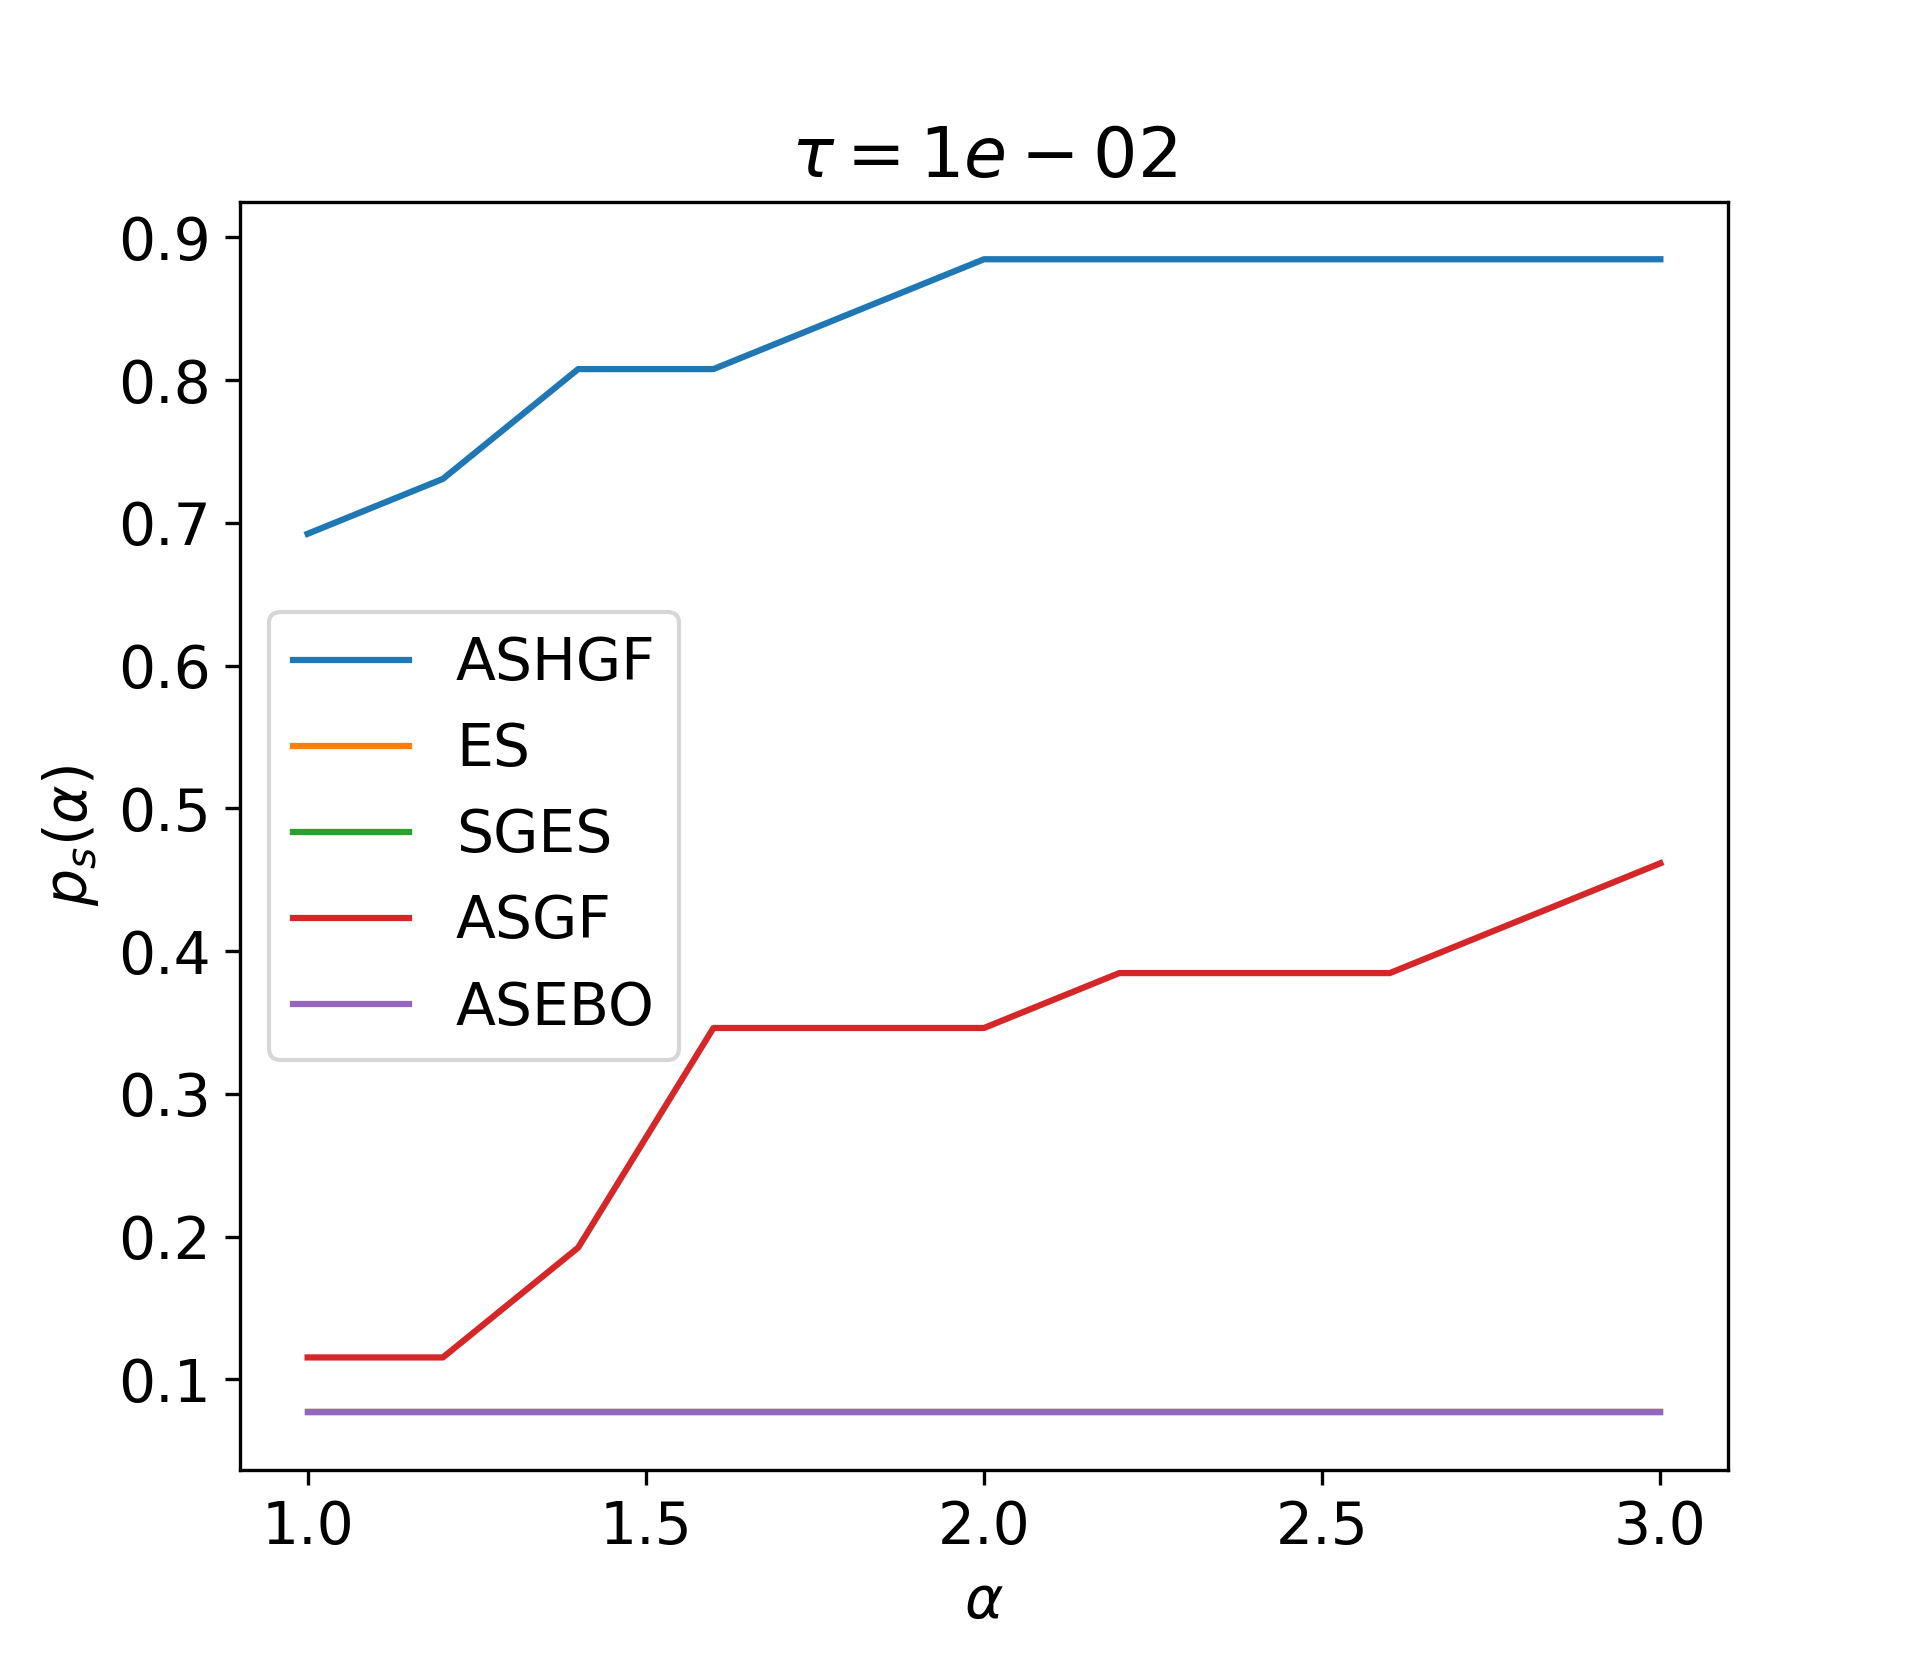
\includegraphics[width=1\textwidth]{figures/performance_profiles/10/performance_profile_10_10000_1e-02.png}
\end{subfigure}%
\begin{subfigure}{0.3\textwidth}
  \centering 
  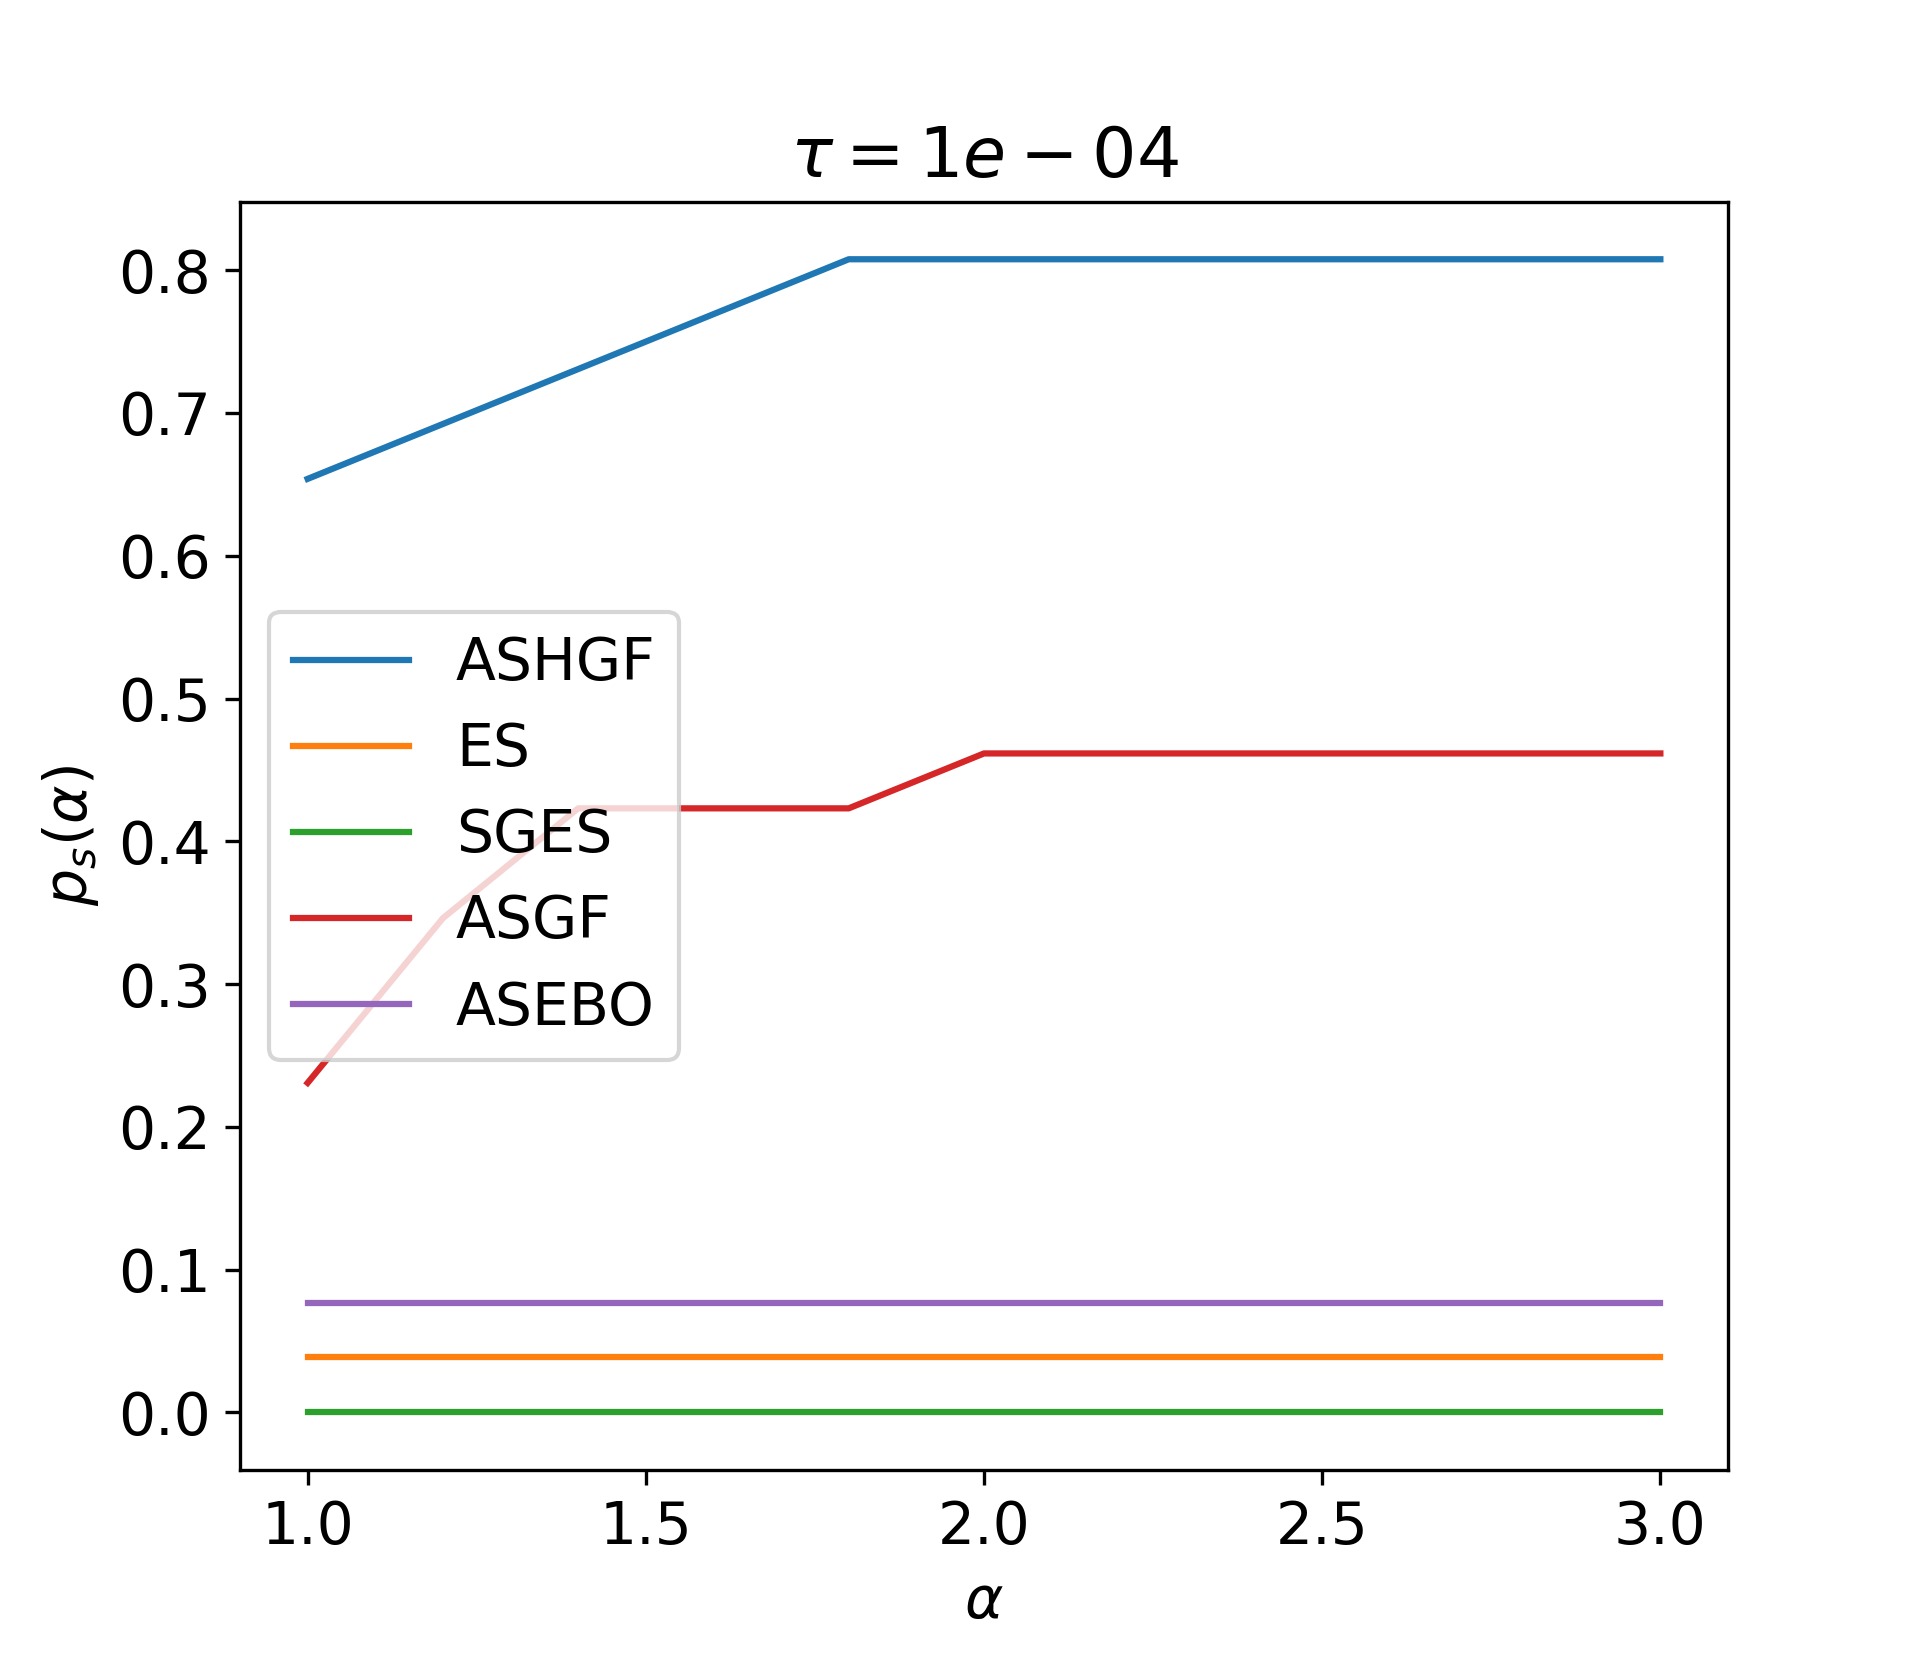
\includegraphics[width=1\textwidth]{figures/performance_profiles/10/performance_profile_10_10000_1e-04.png}
\end{subfigure}
\begin{subfigure}{0.3\textwidth}
  \centering 
  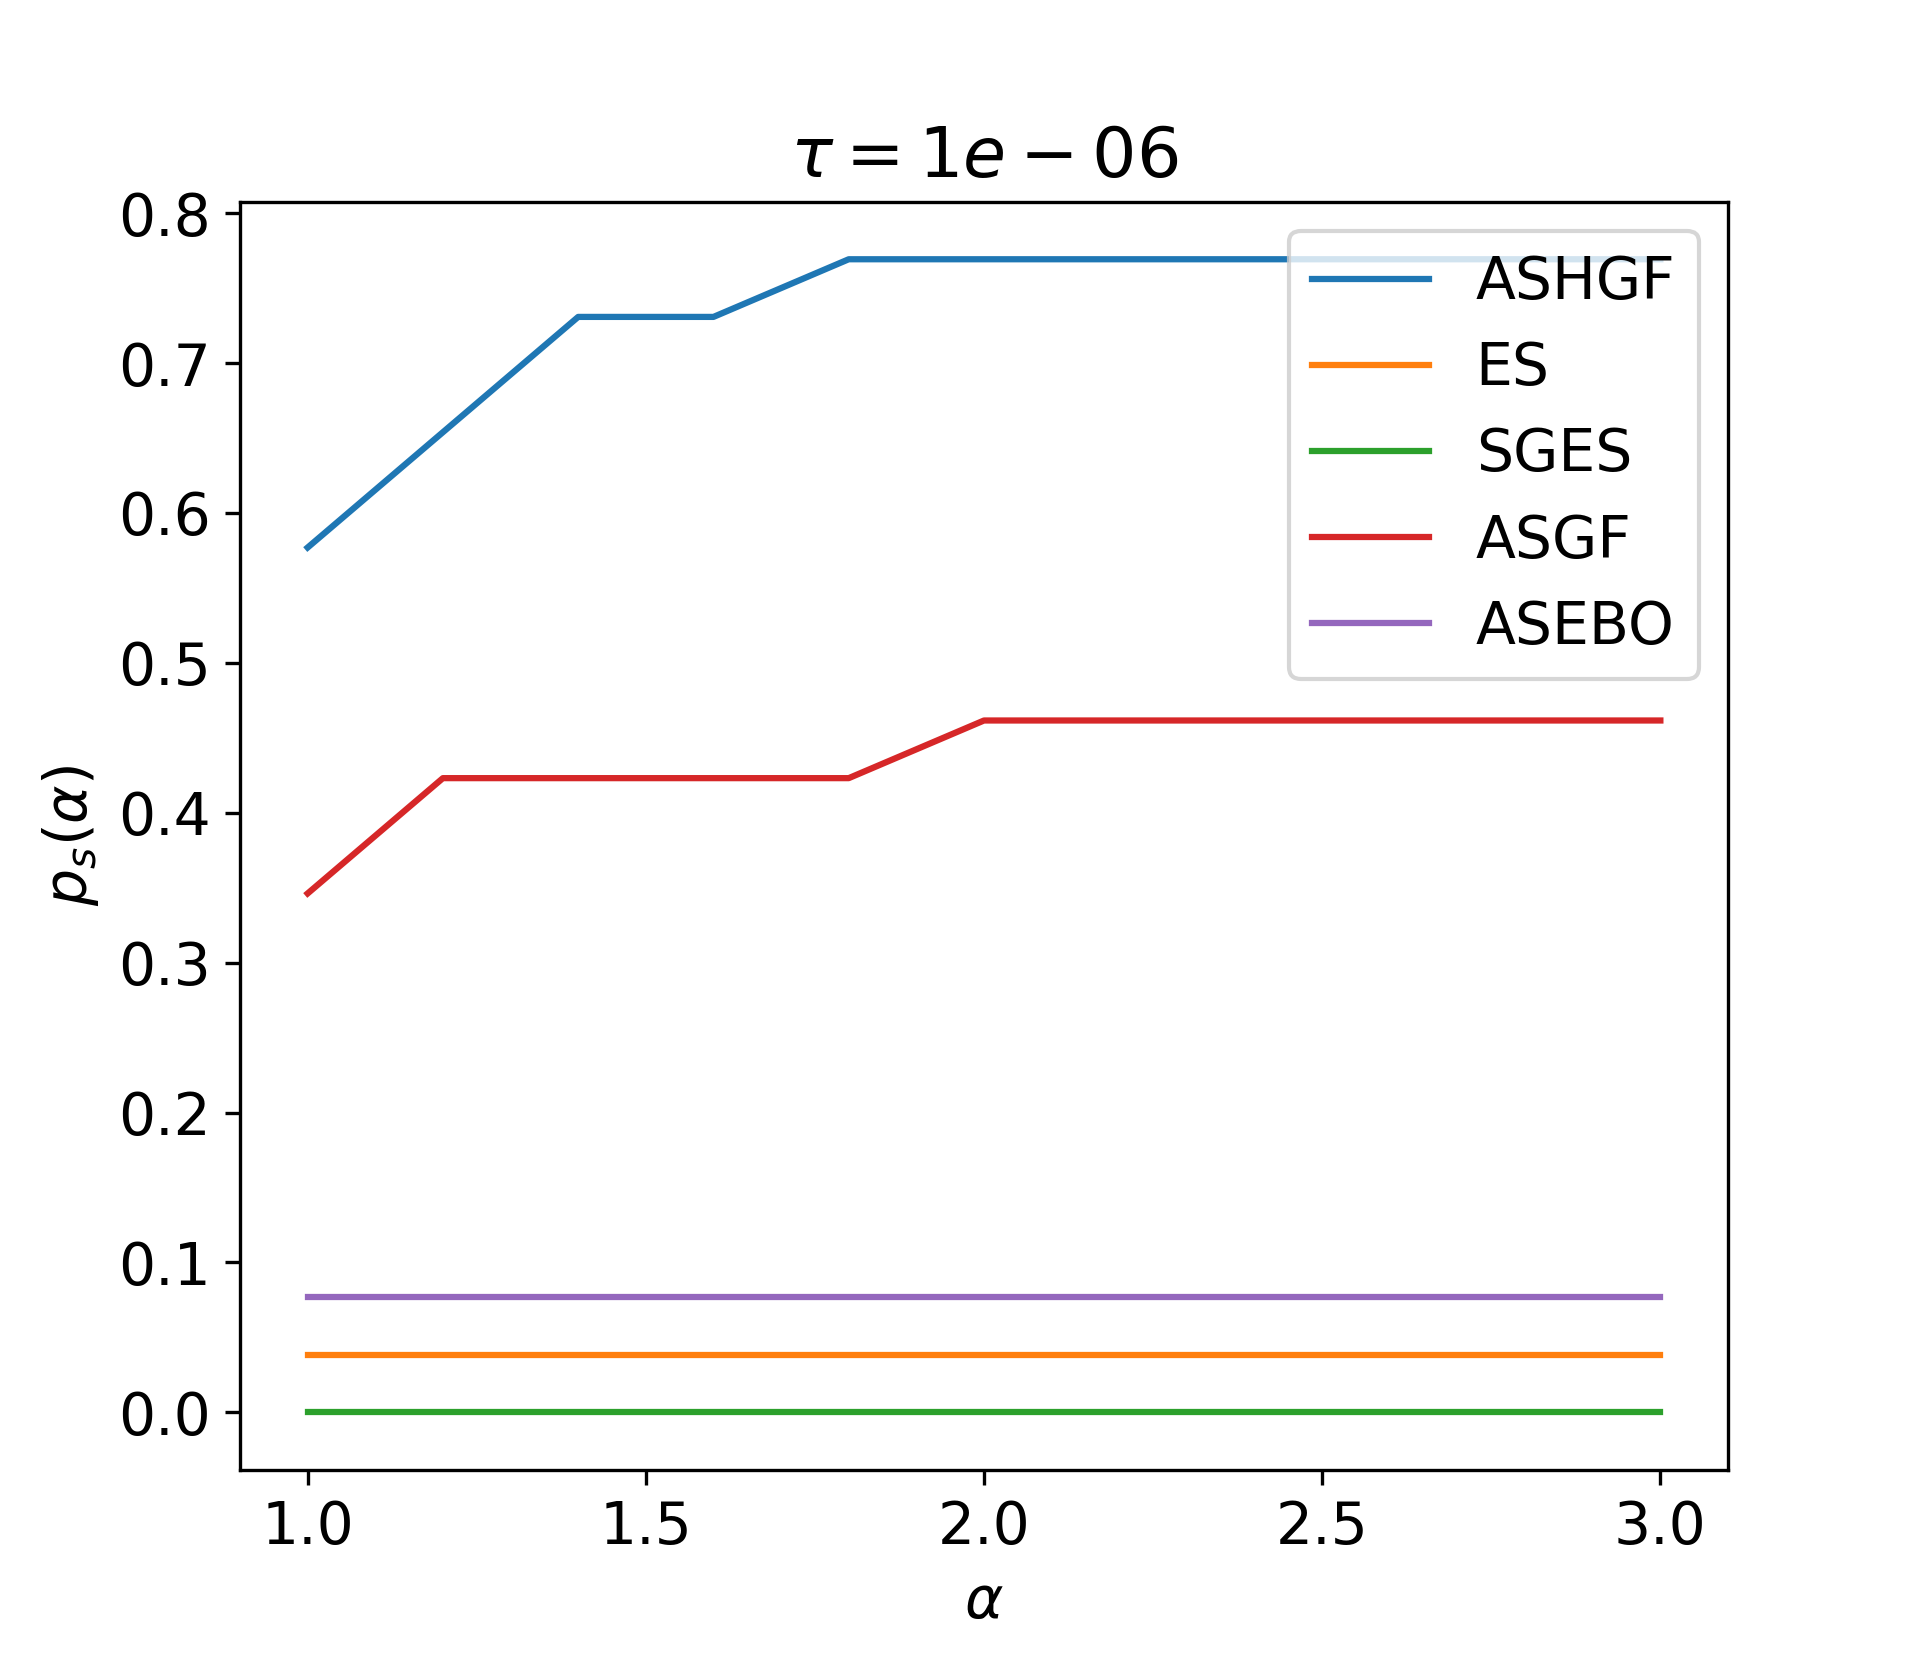
\includegraphics[width=1\textwidth]{figures/performance_profiles/10/performance_profile_10_10000_1e-06.png}
\end{subfigure}
\centering
\begin{subfigure}{0.3\textwidth}
  \centering 
  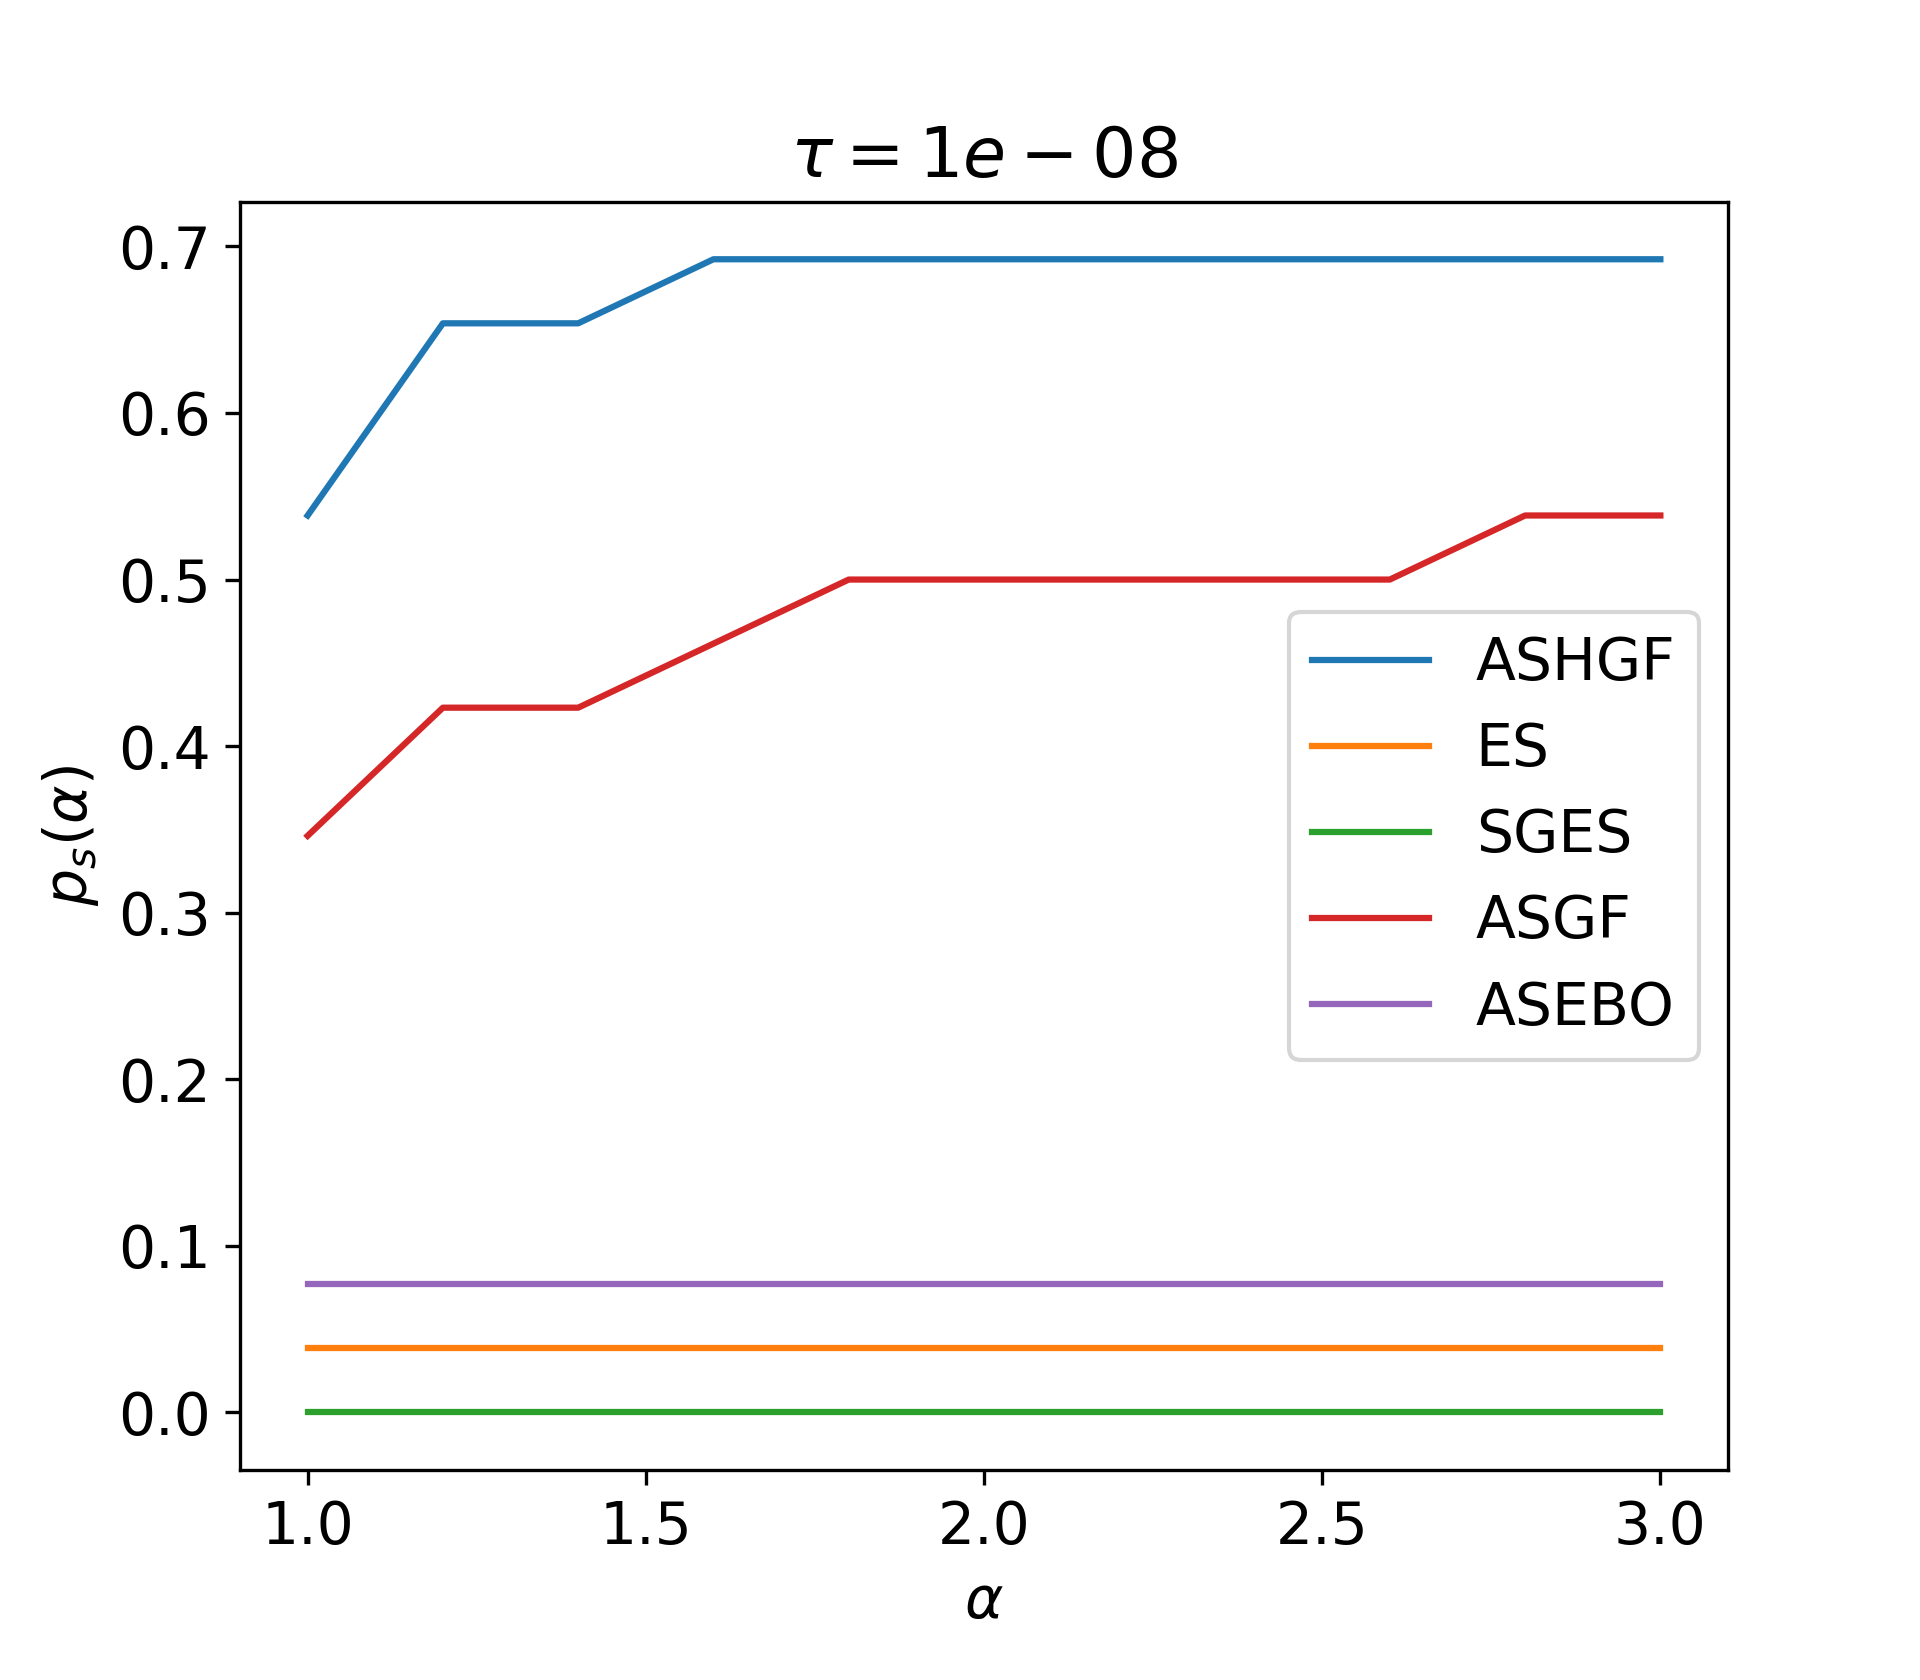
\includegraphics[width=1\textwidth]{figures/performance_profiles/10/performance_profile_10_10000_1e-08.png}
\end{subfigure}%
\begin{subfigure}{0.3\textwidth}
  \centering 
  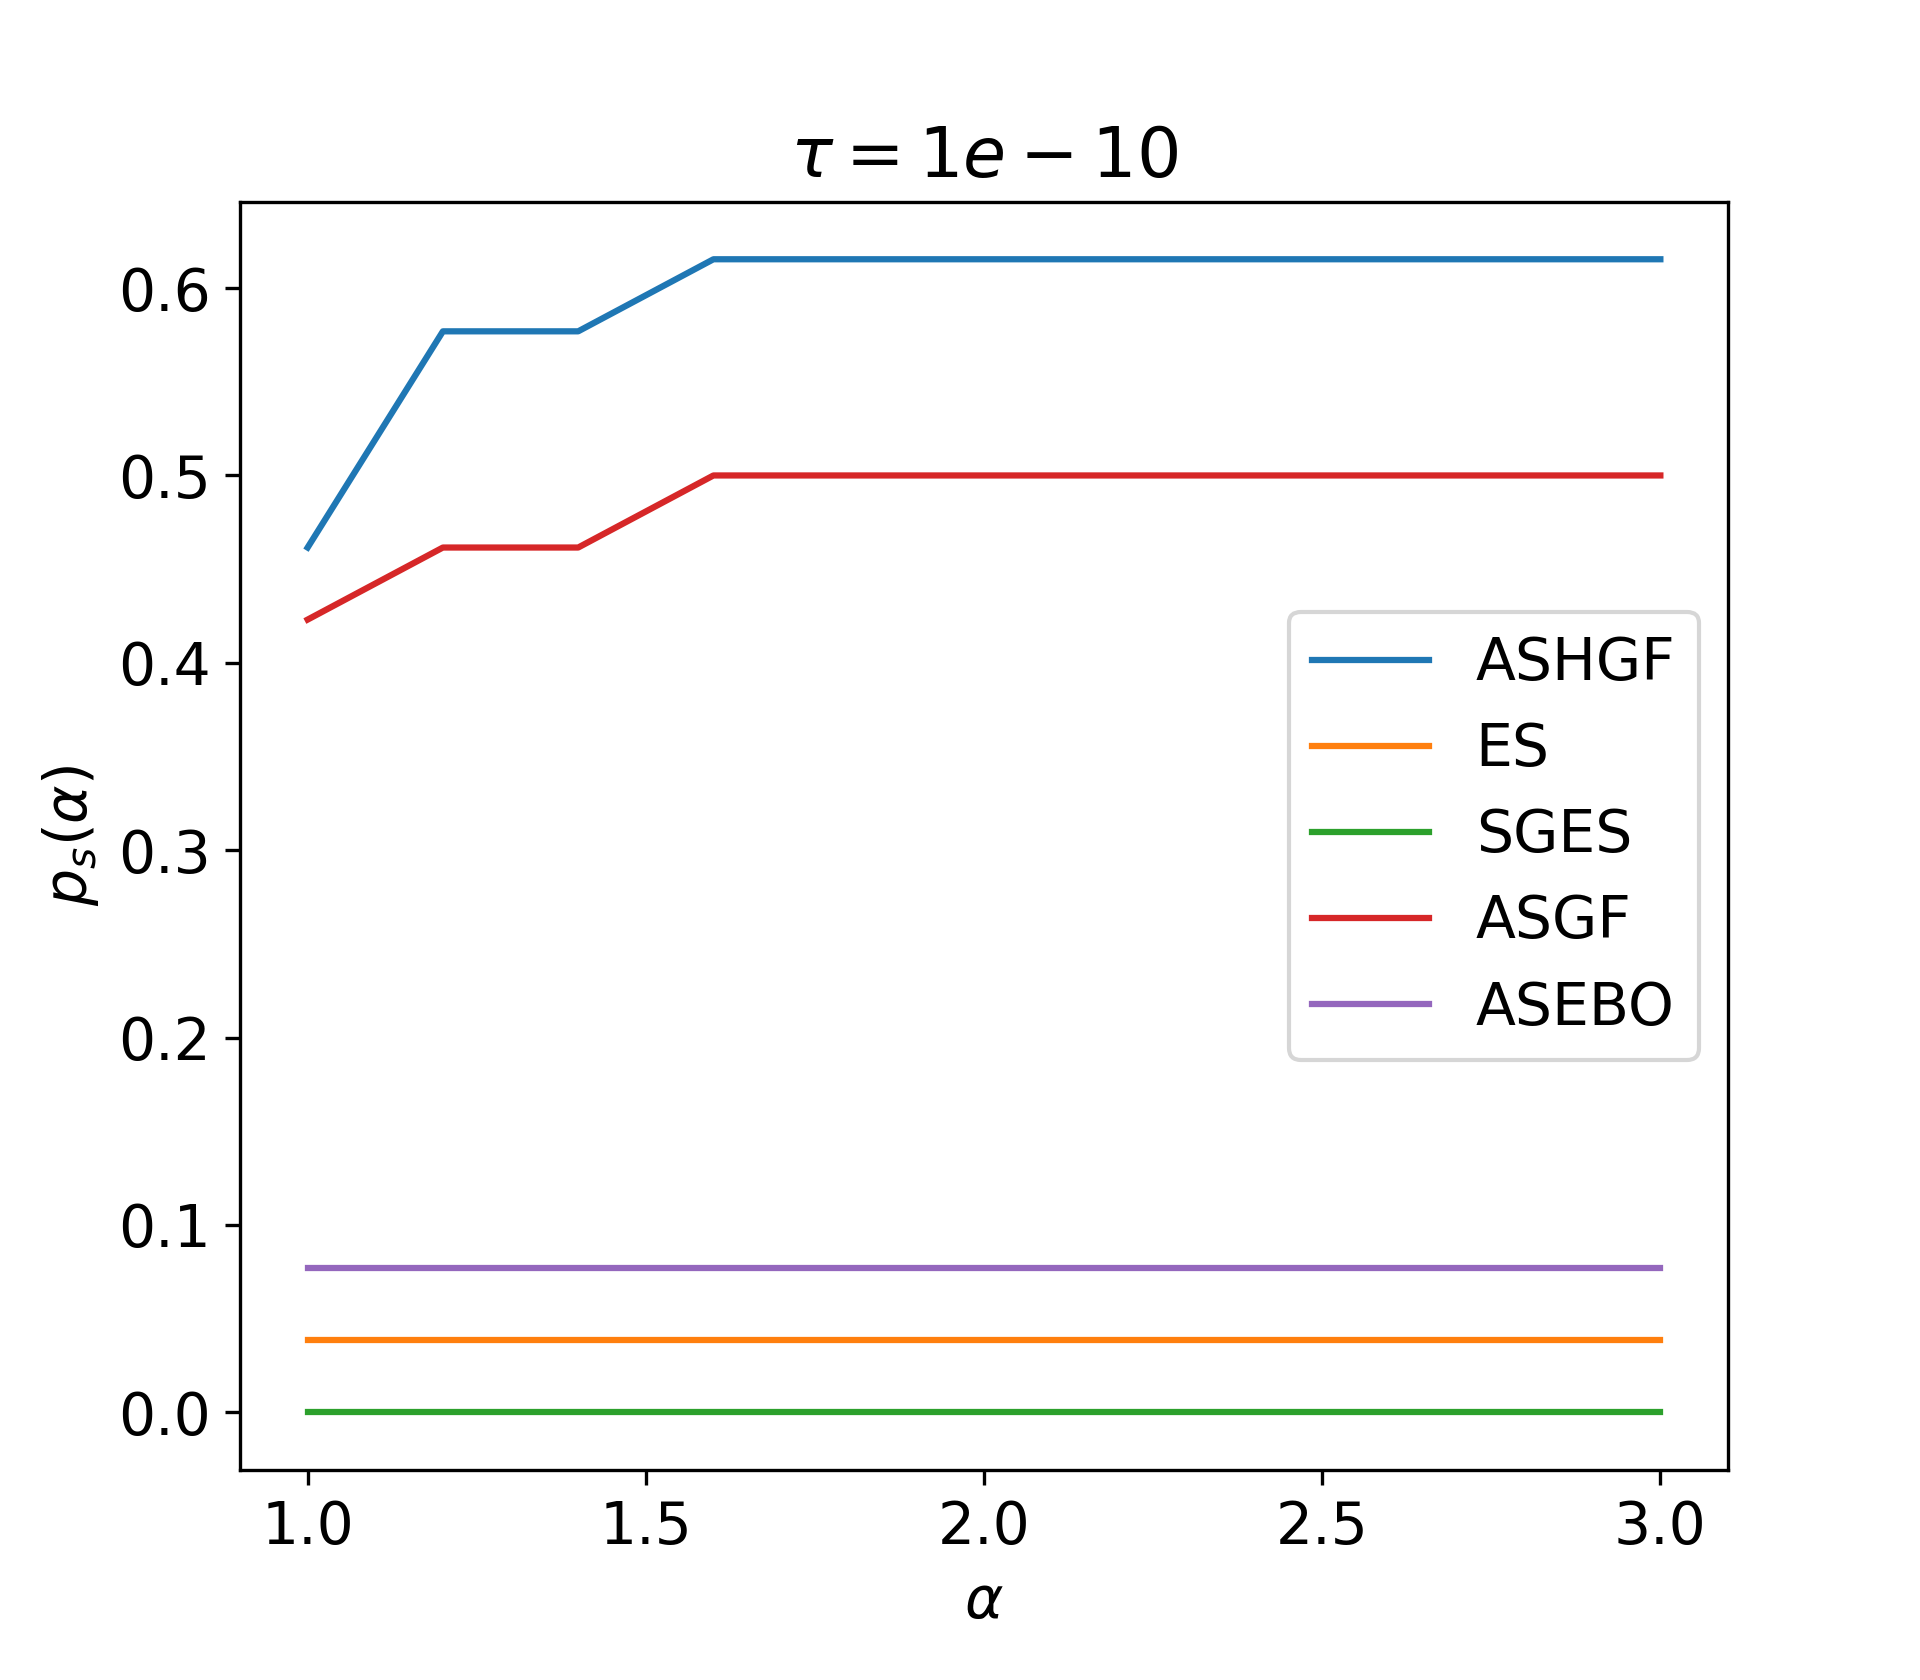
\includegraphics[width=1\textwidth]{figures/performance_profiles/10/performance_profile_10_10000_1e-10.png}
\end{subfigure}
\caption{Performance profiles with $\mu_L = 10^{4}$}
\label{PerformanceProfiles10Mu10000}
\end{figure}

\begin{figure}[H]
\centering
\begin{subfigure}{0.3\textwidth}
  \centering 
  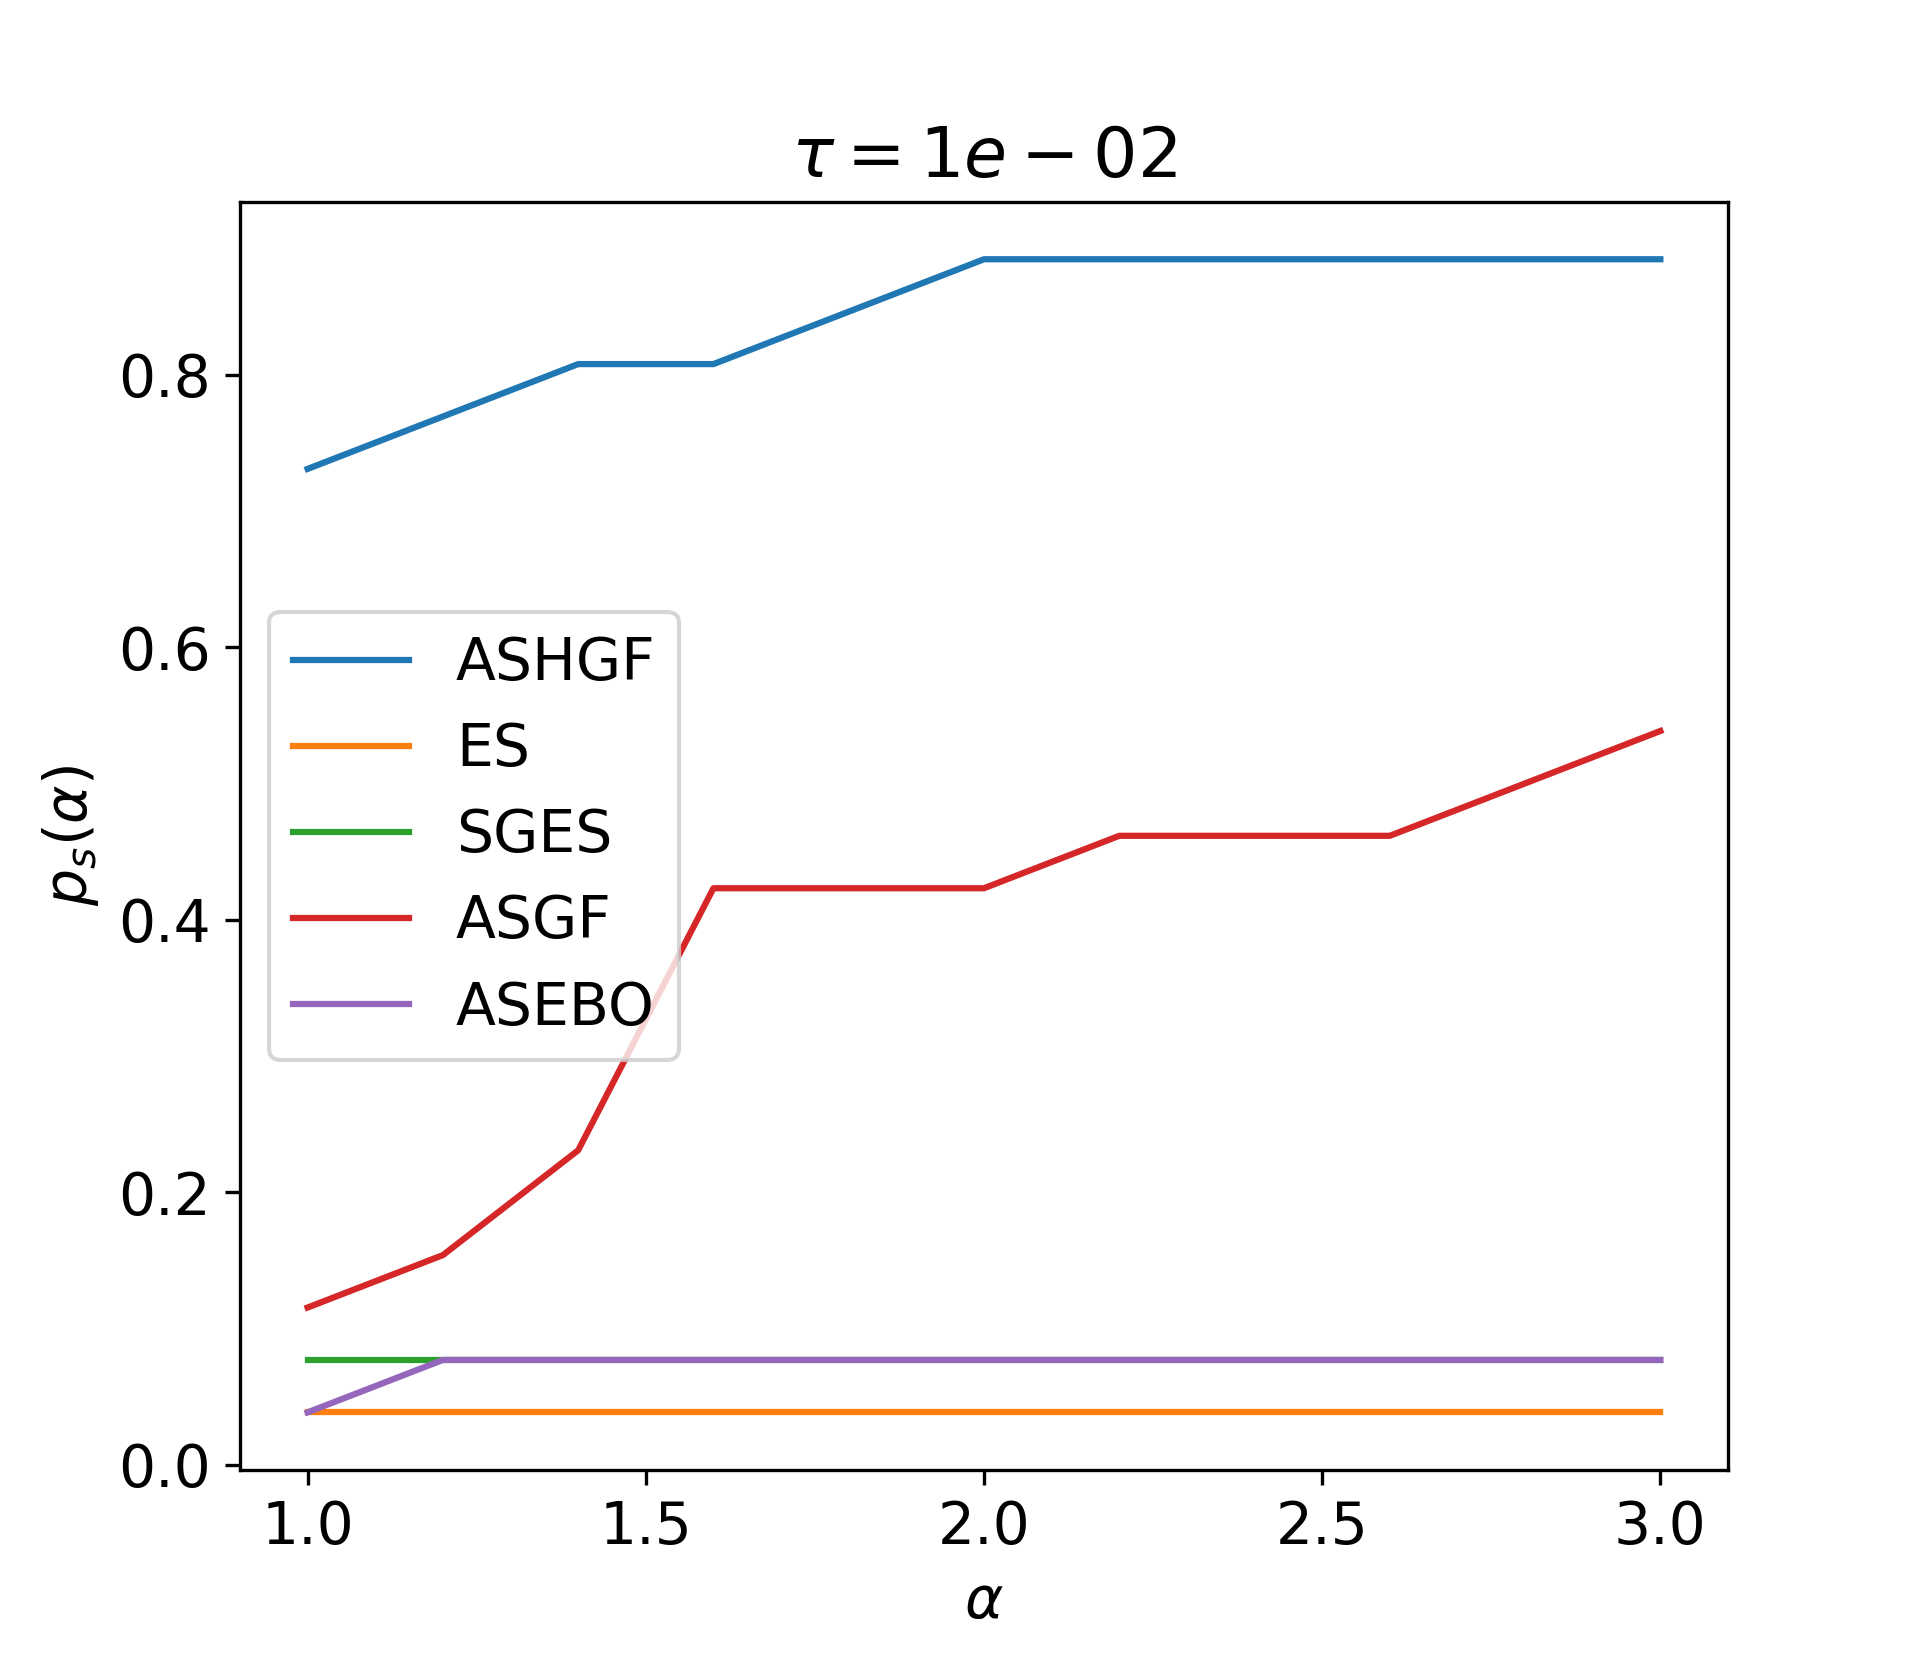
\includegraphics[width=1\textwidth]{figures/performance_profiles/10/performance_profile_10_100000_1e-02.png}
\end{subfigure}%
\begin{subfigure}{0.3\textwidth}
  \centering 
  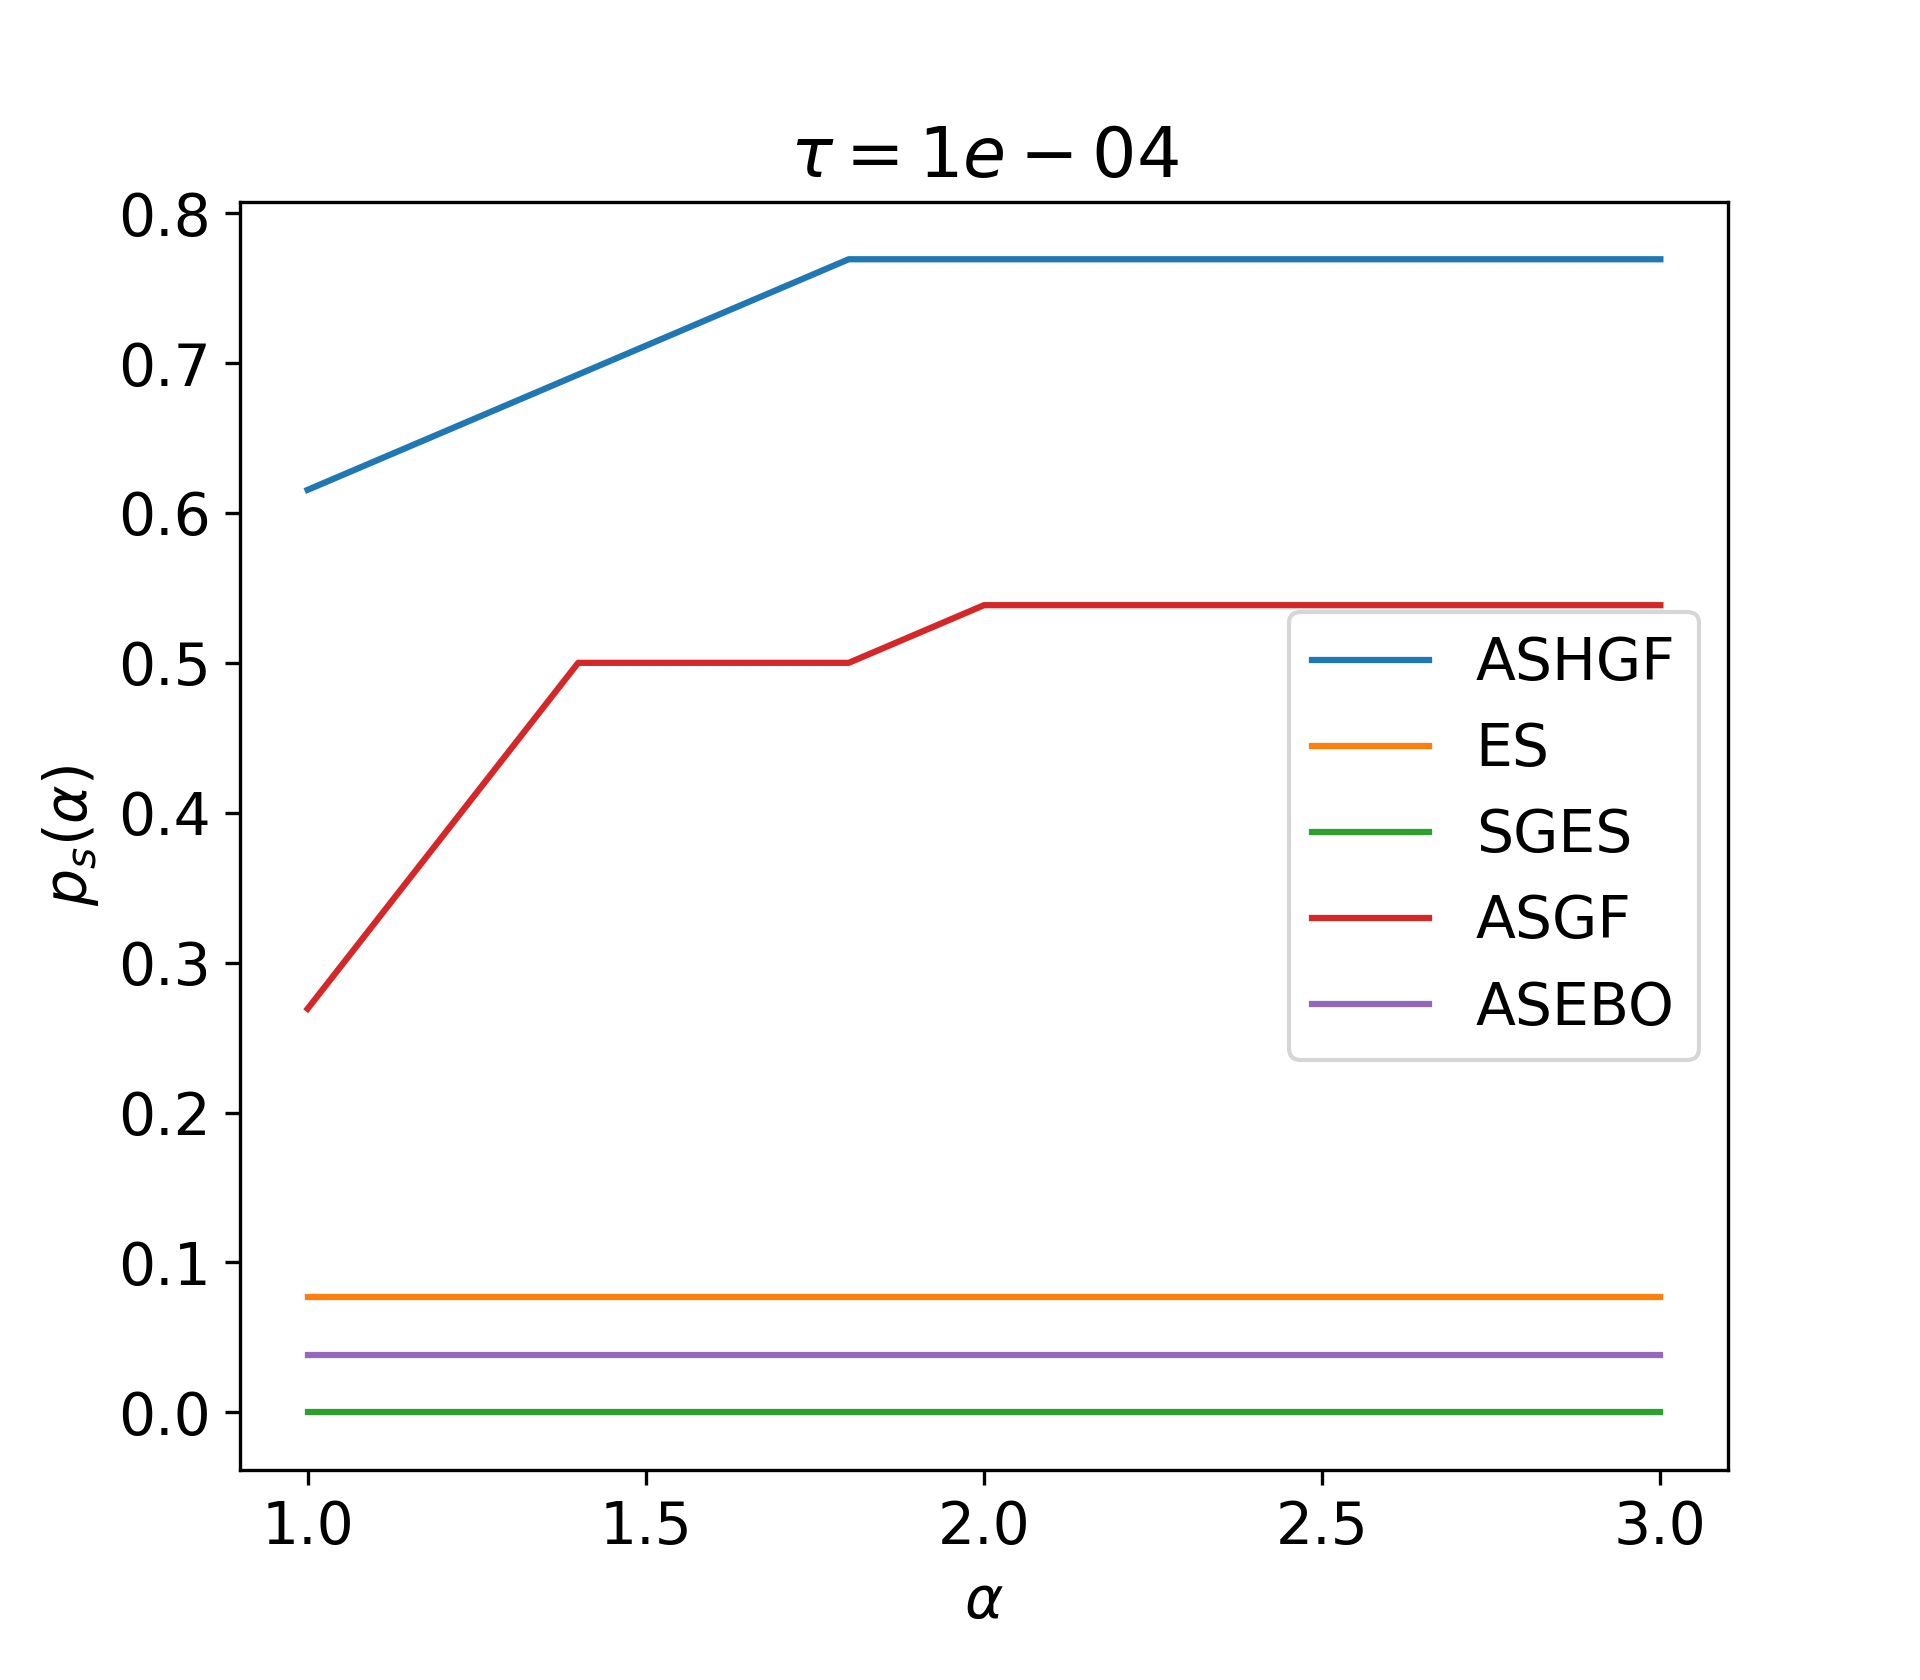
\includegraphics[width=1\textwidth]{figures/performance_profiles/10/performance_profile_10_100000_1e-04.png}
\end{subfigure}
\begin{subfigure}{0.3\textwidth}
  \centering 
  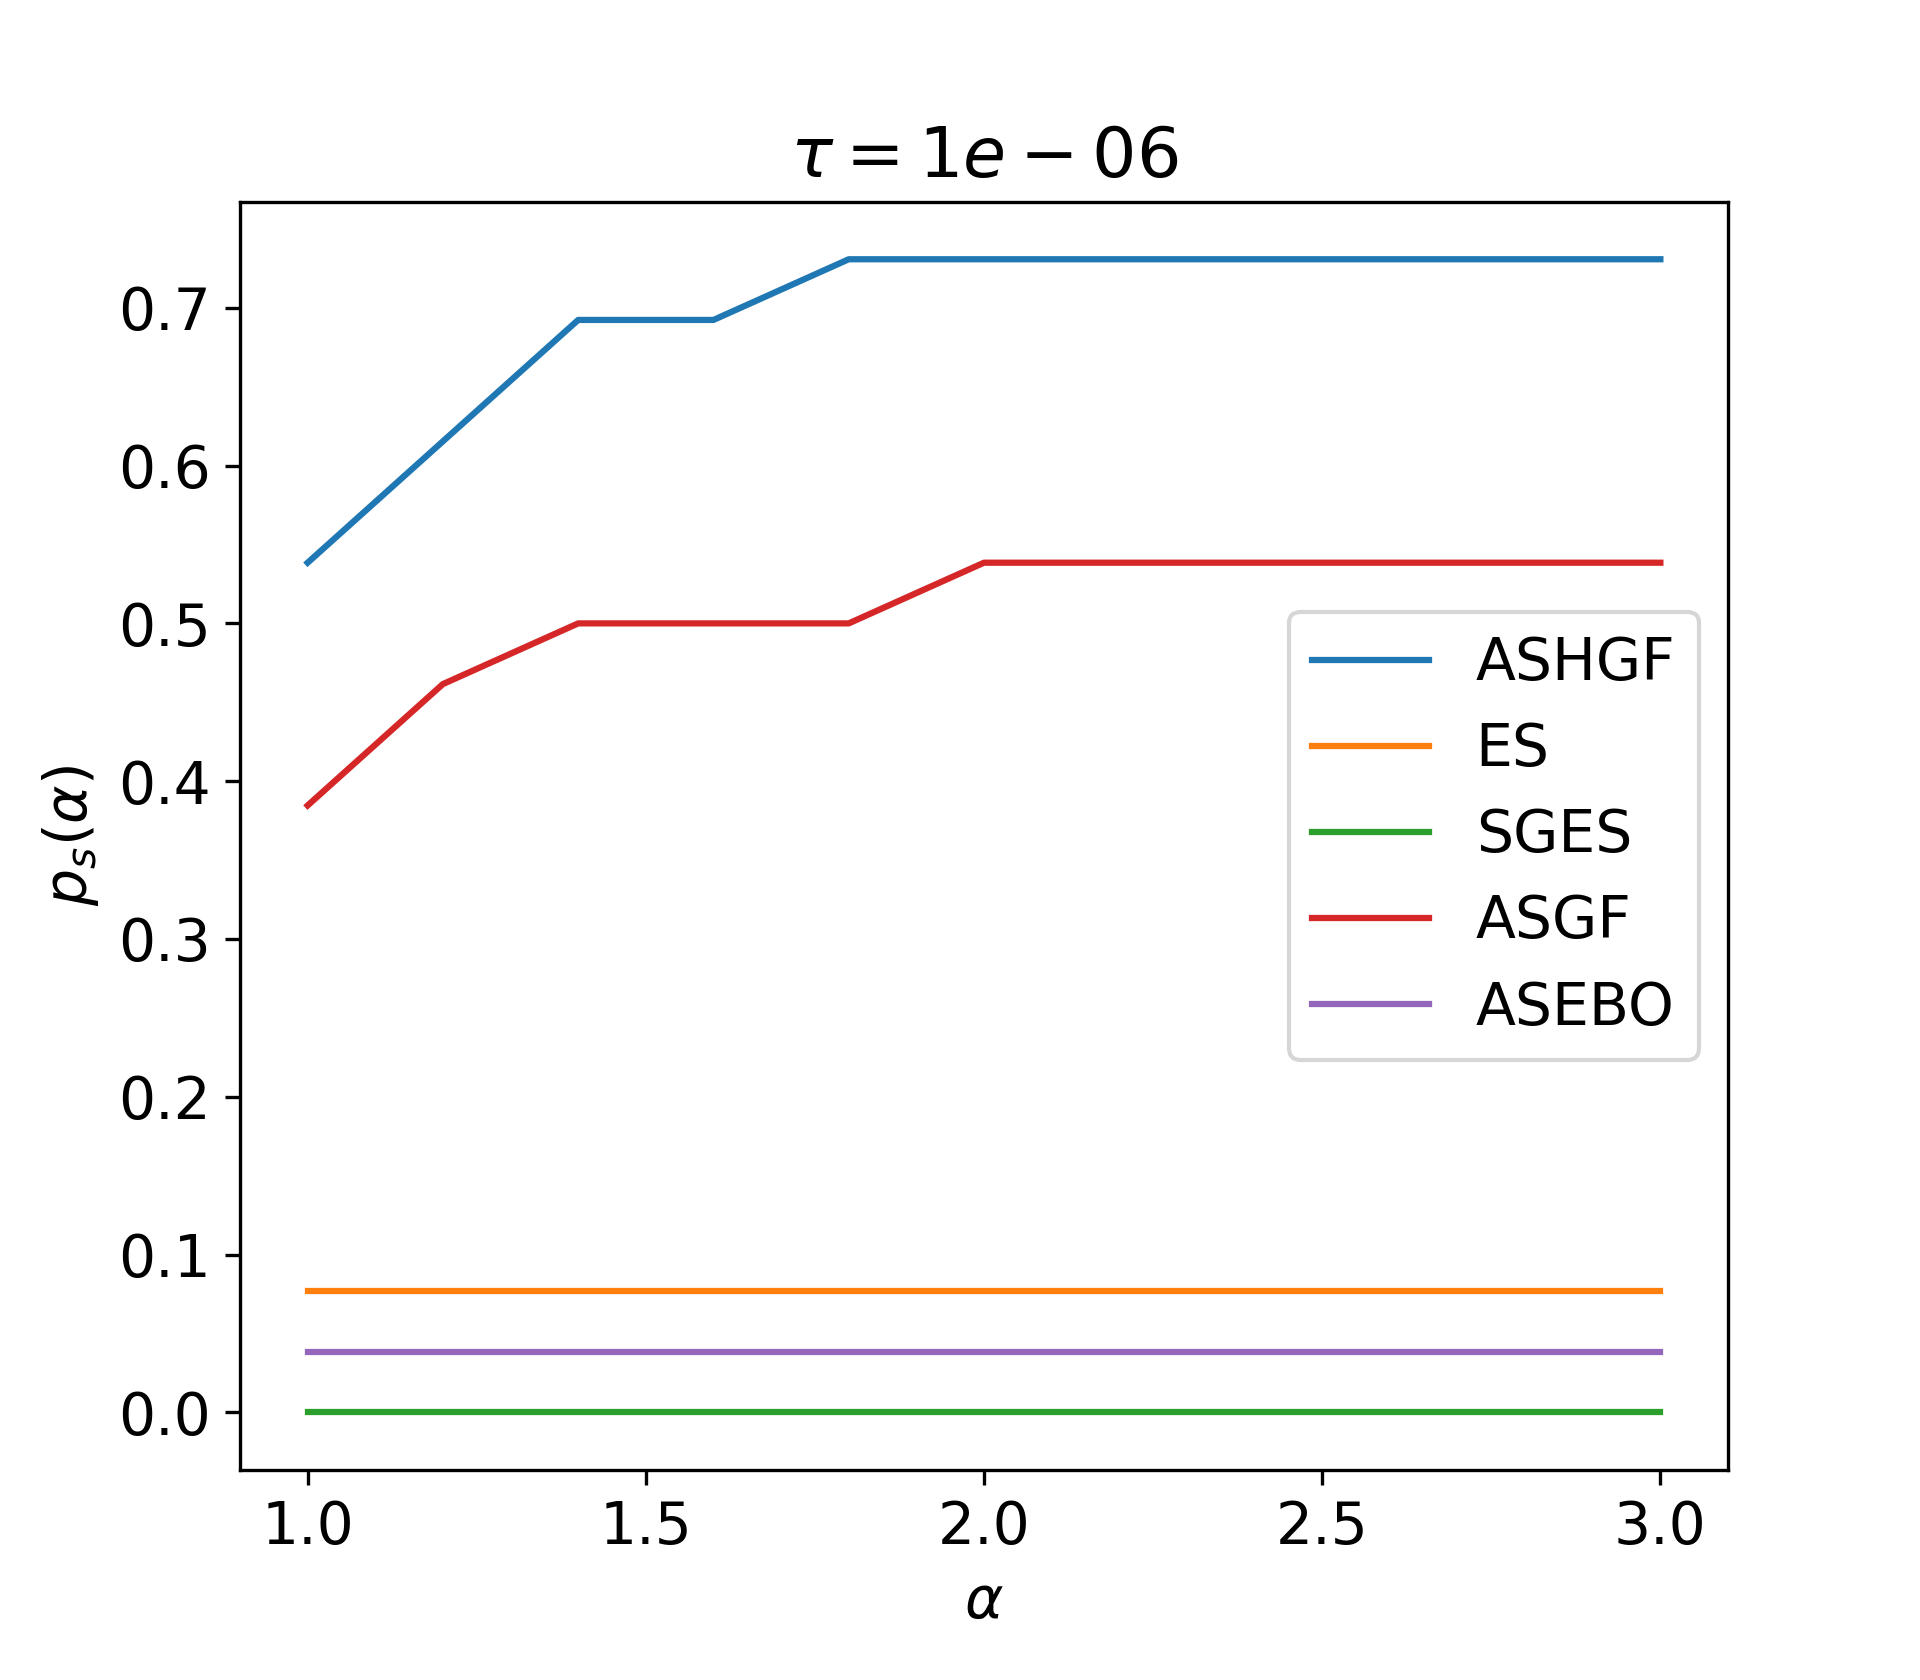
\includegraphics[width=1\textwidth]{figures/performance_profiles/10/performance_profile_10_100000_1e-06.png}
\end{subfigure}
\centering
\begin{subfigure}{0.3\textwidth}
  \centering 
  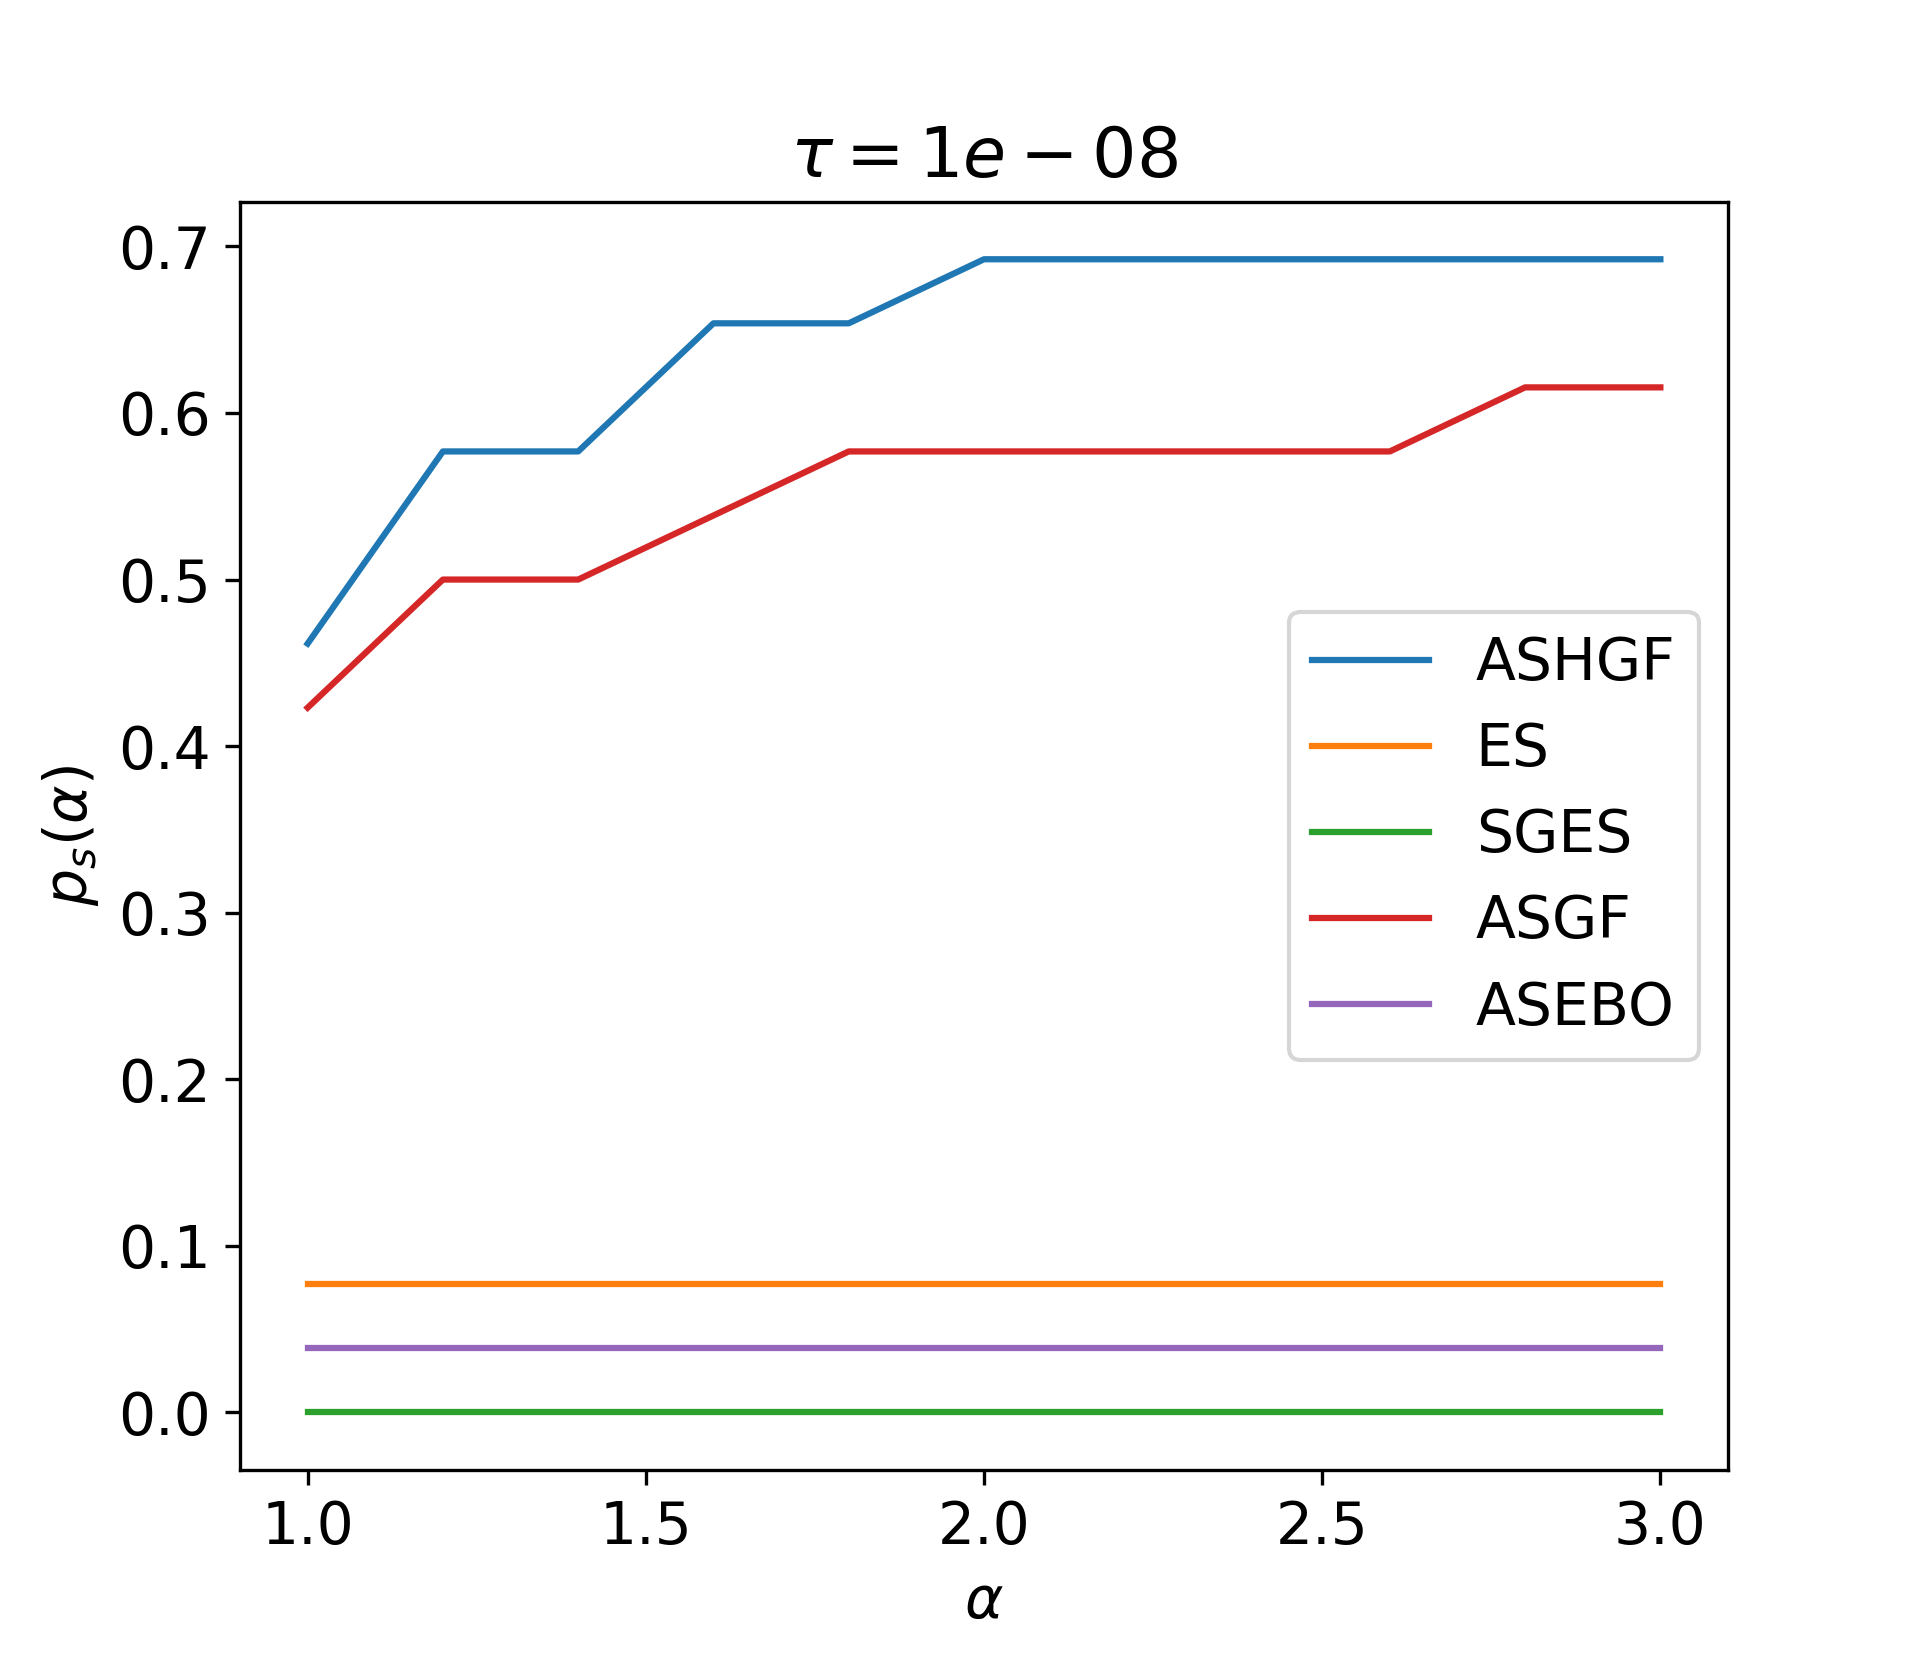
\includegraphics[width=1\textwidth]{figures/performance_profiles/10/performance_profile_10_100000_1e-08.png}
\end{subfigure}%
\begin{subfigure}{0.3\textwidth}
  \centering 
  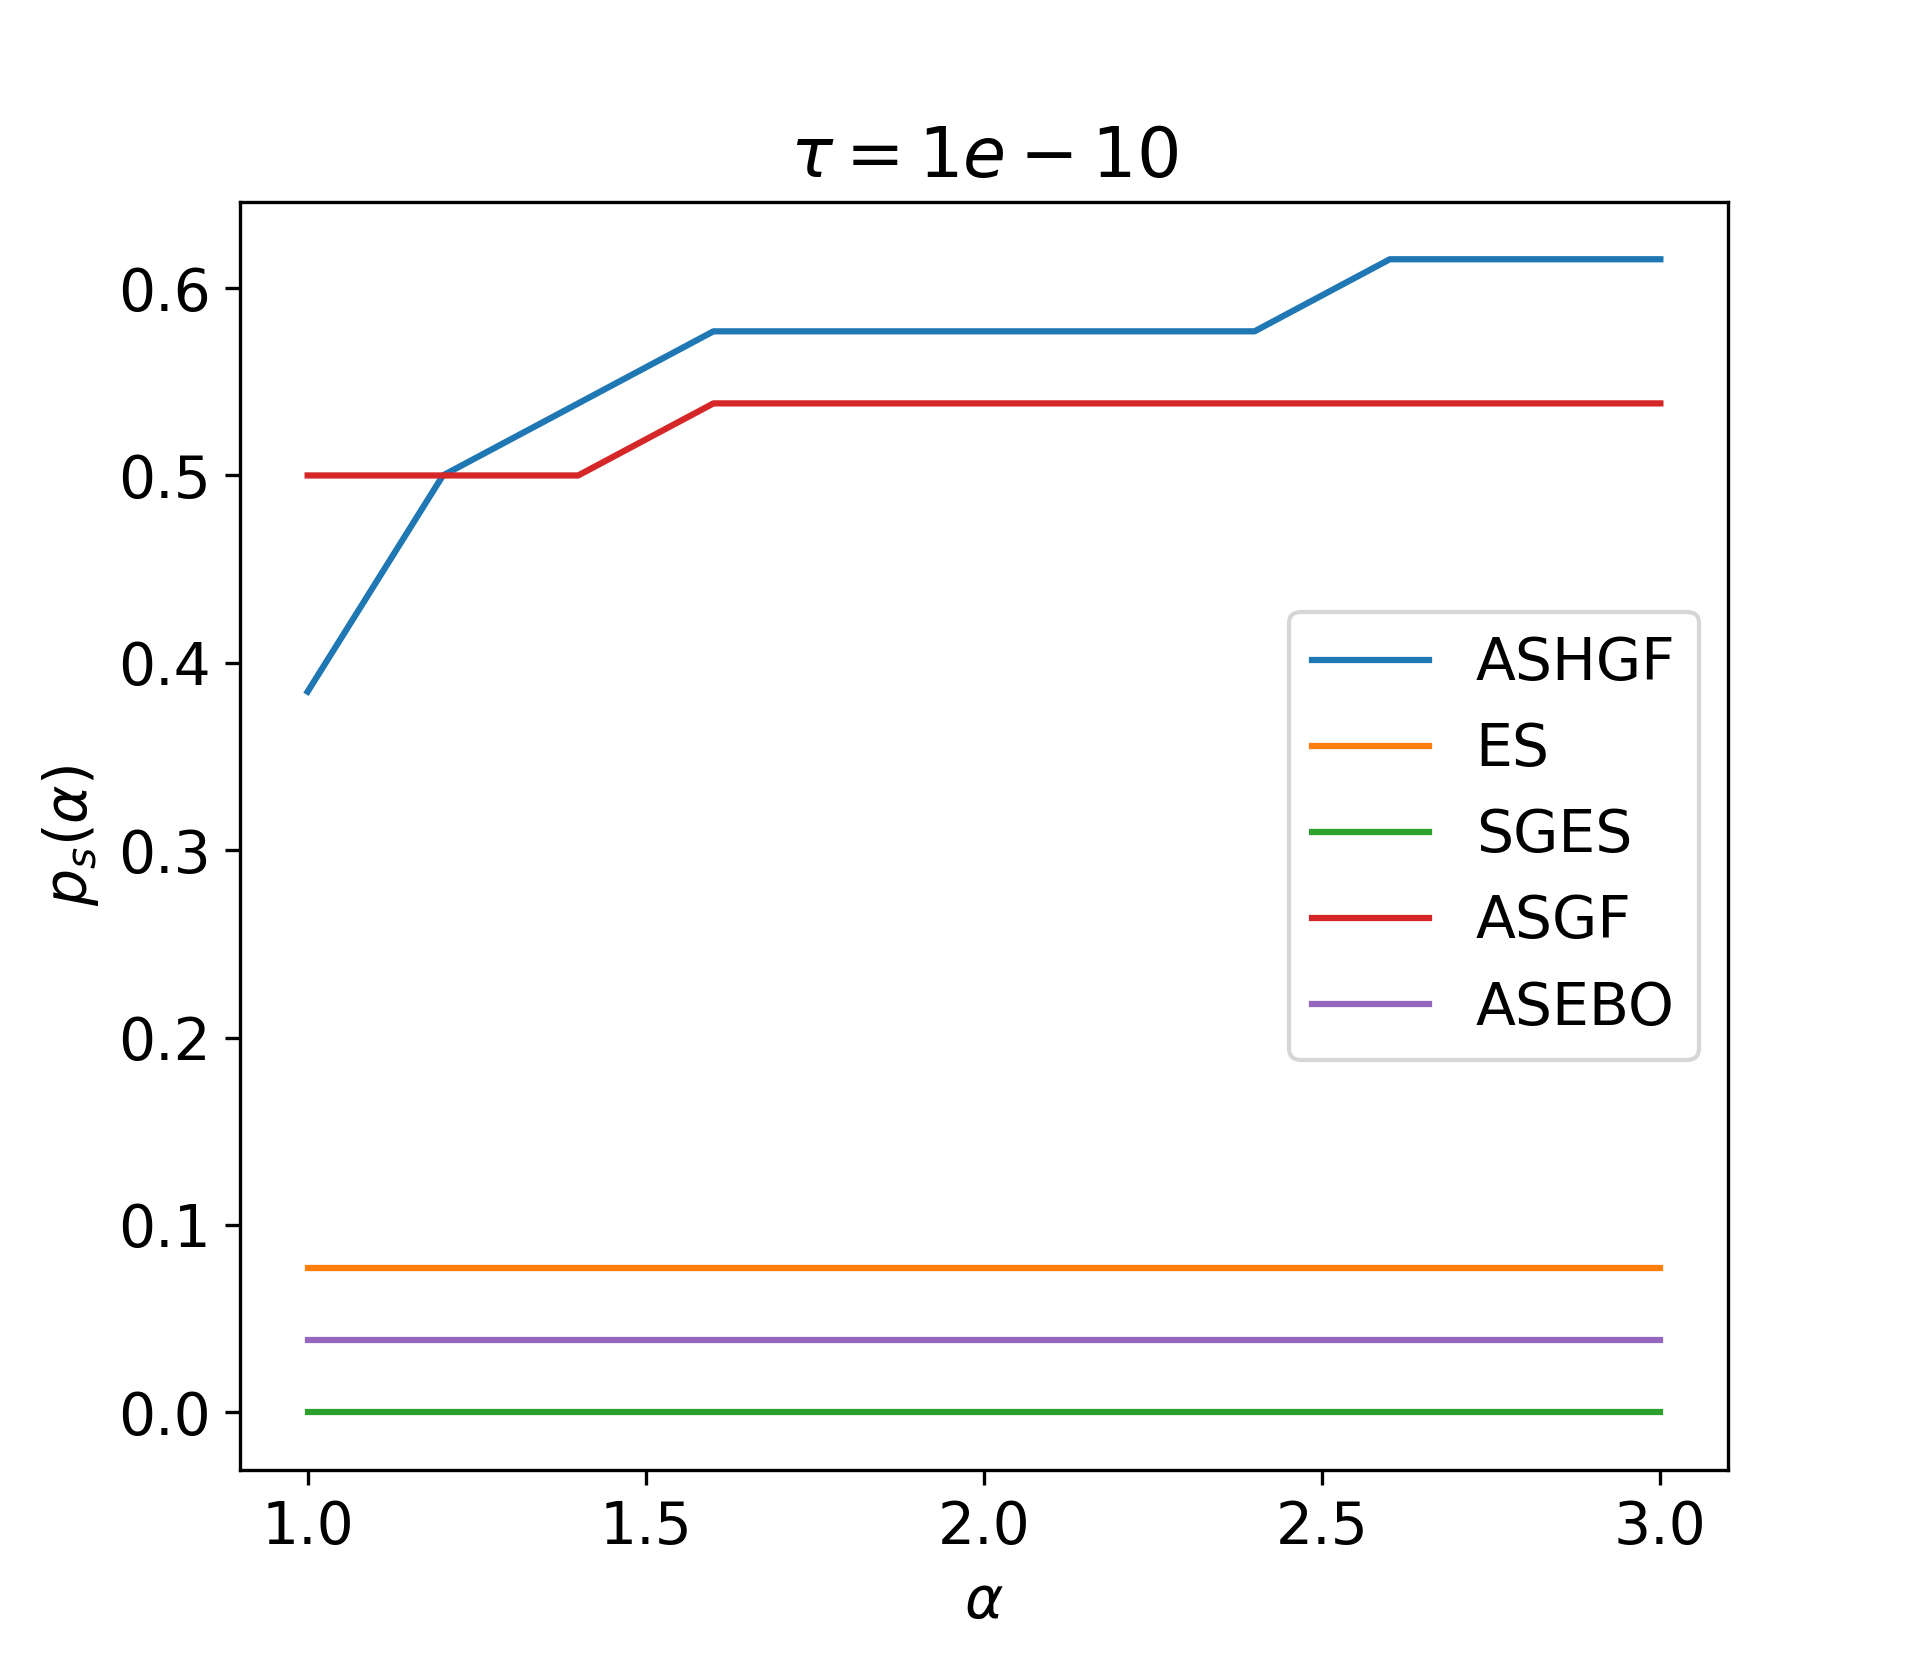
\includegraphics[width=1\textwidth]{figures/performance_profiles/10/performance_profile_10_100000_1e-10.png}
\end{subfigure}
\caption{Performance profiles with $\mu_L = 10^{5}$}
\label{PerformanceProfiles10Mu100000}
\end{figure}

\begin{figure}[H]
\centering
\begin{subfigure}{0.3\textwidth}
  \centering 
  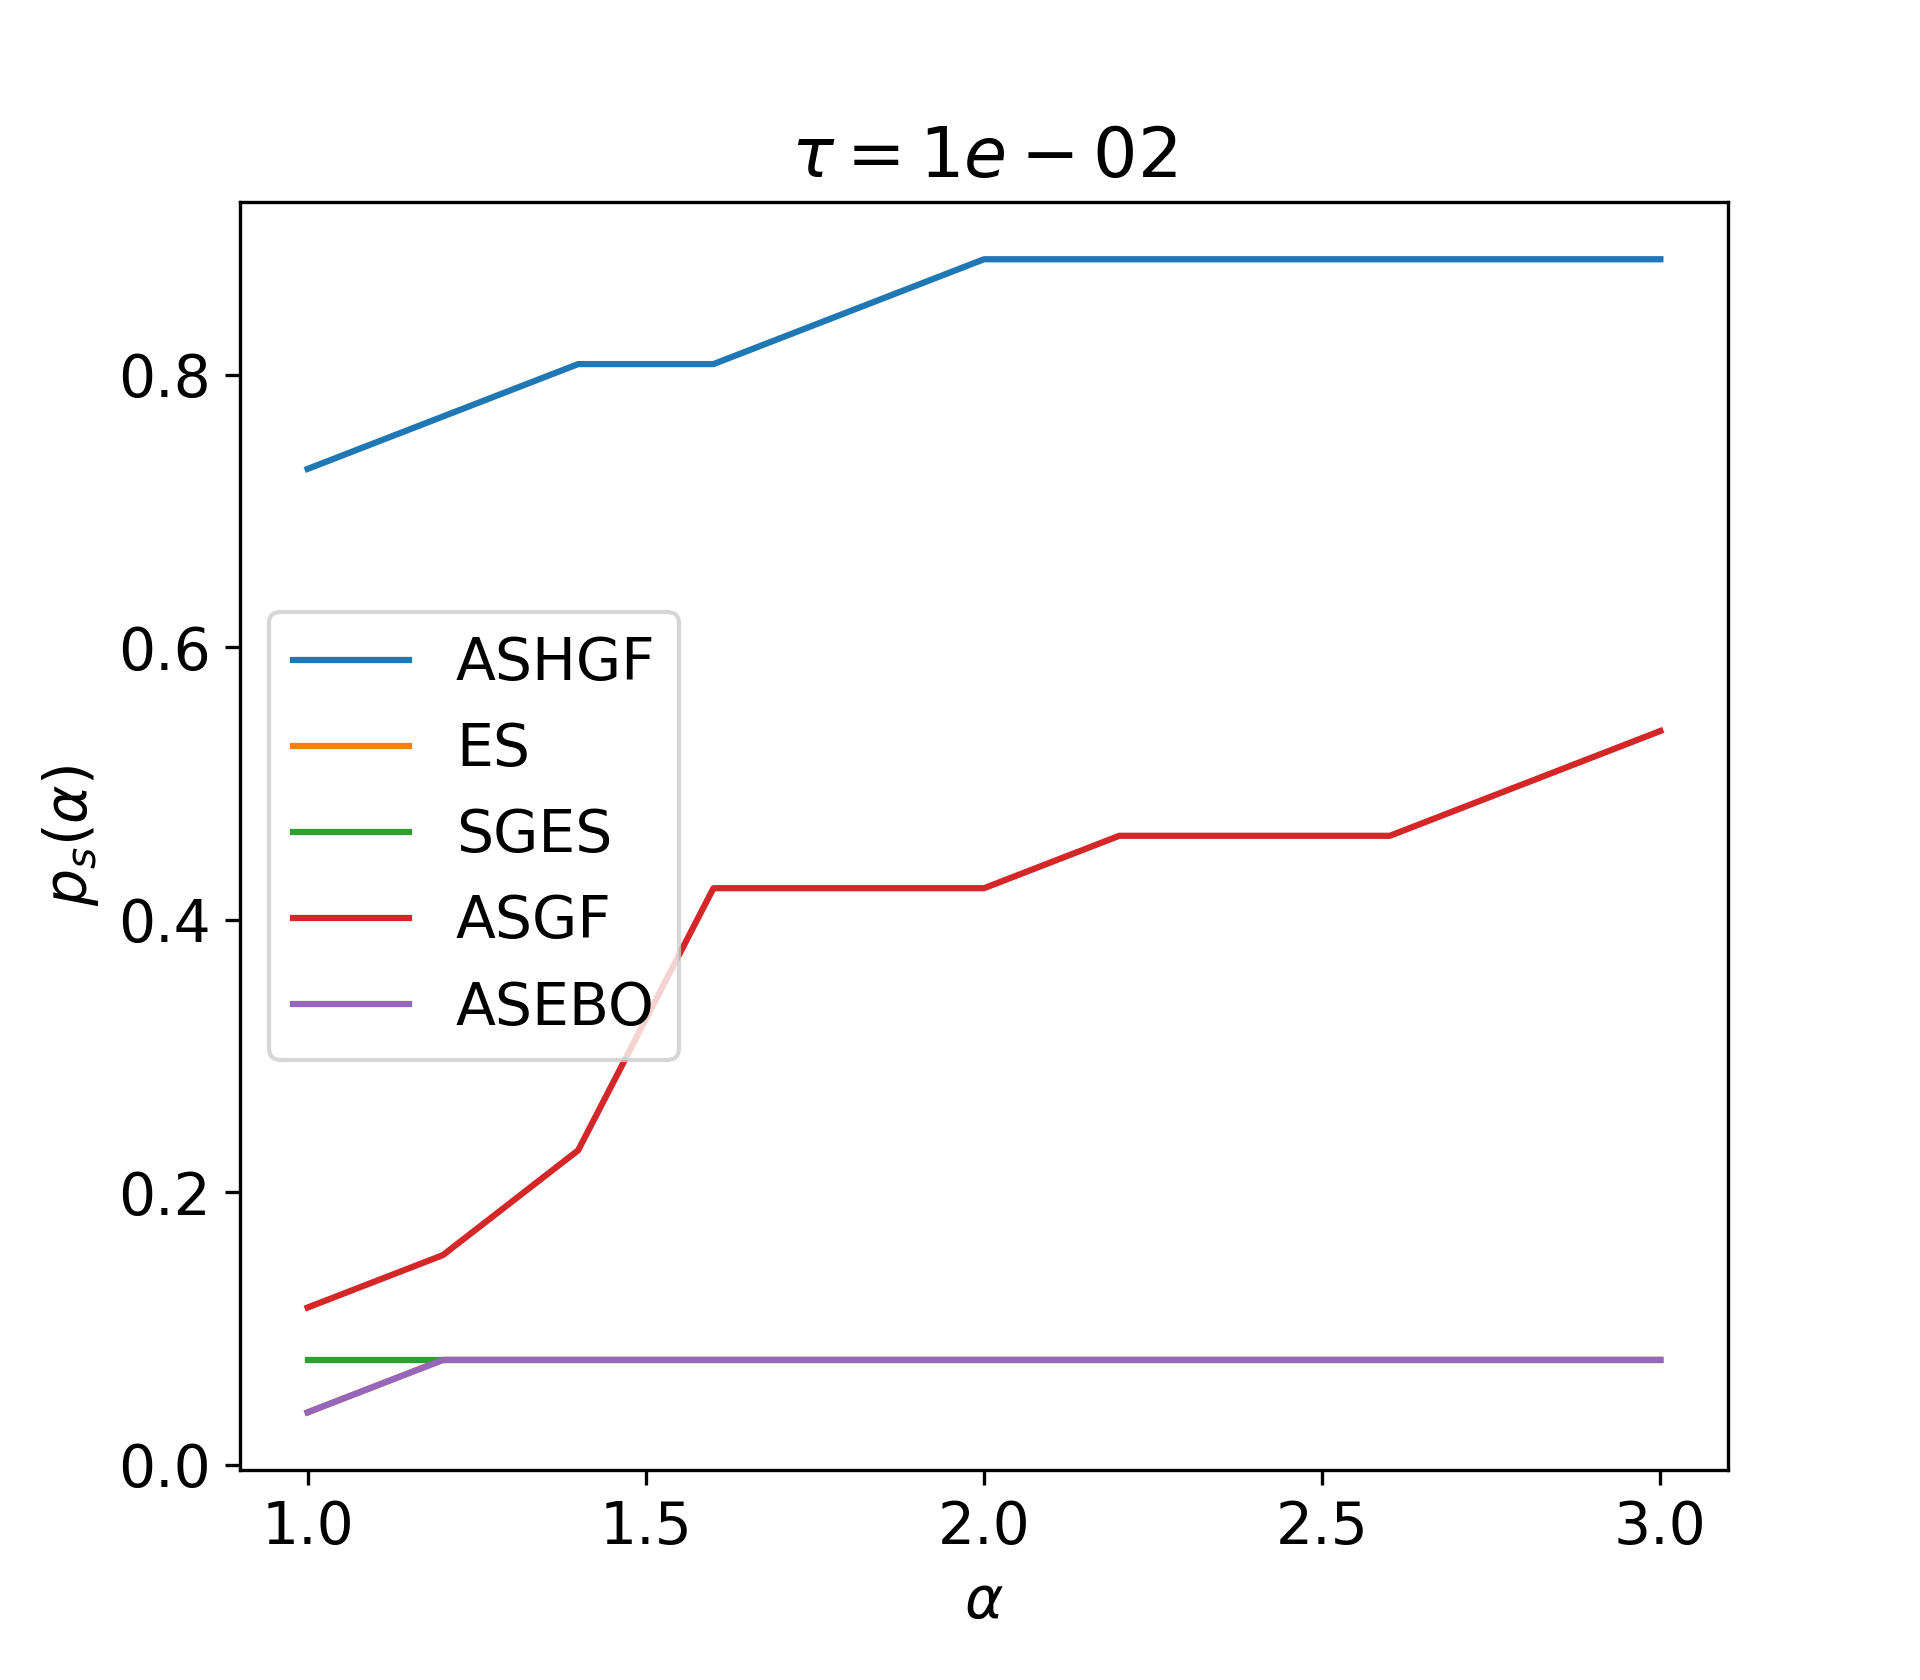
\includegraphics[width=1\textwidth]{figures/performance_profiles/10/performance_profile_10_1000000_1e-02.png}
\end{subfigure}%
\begin{subfigure}{0.3\textwidth}
  \centering 
  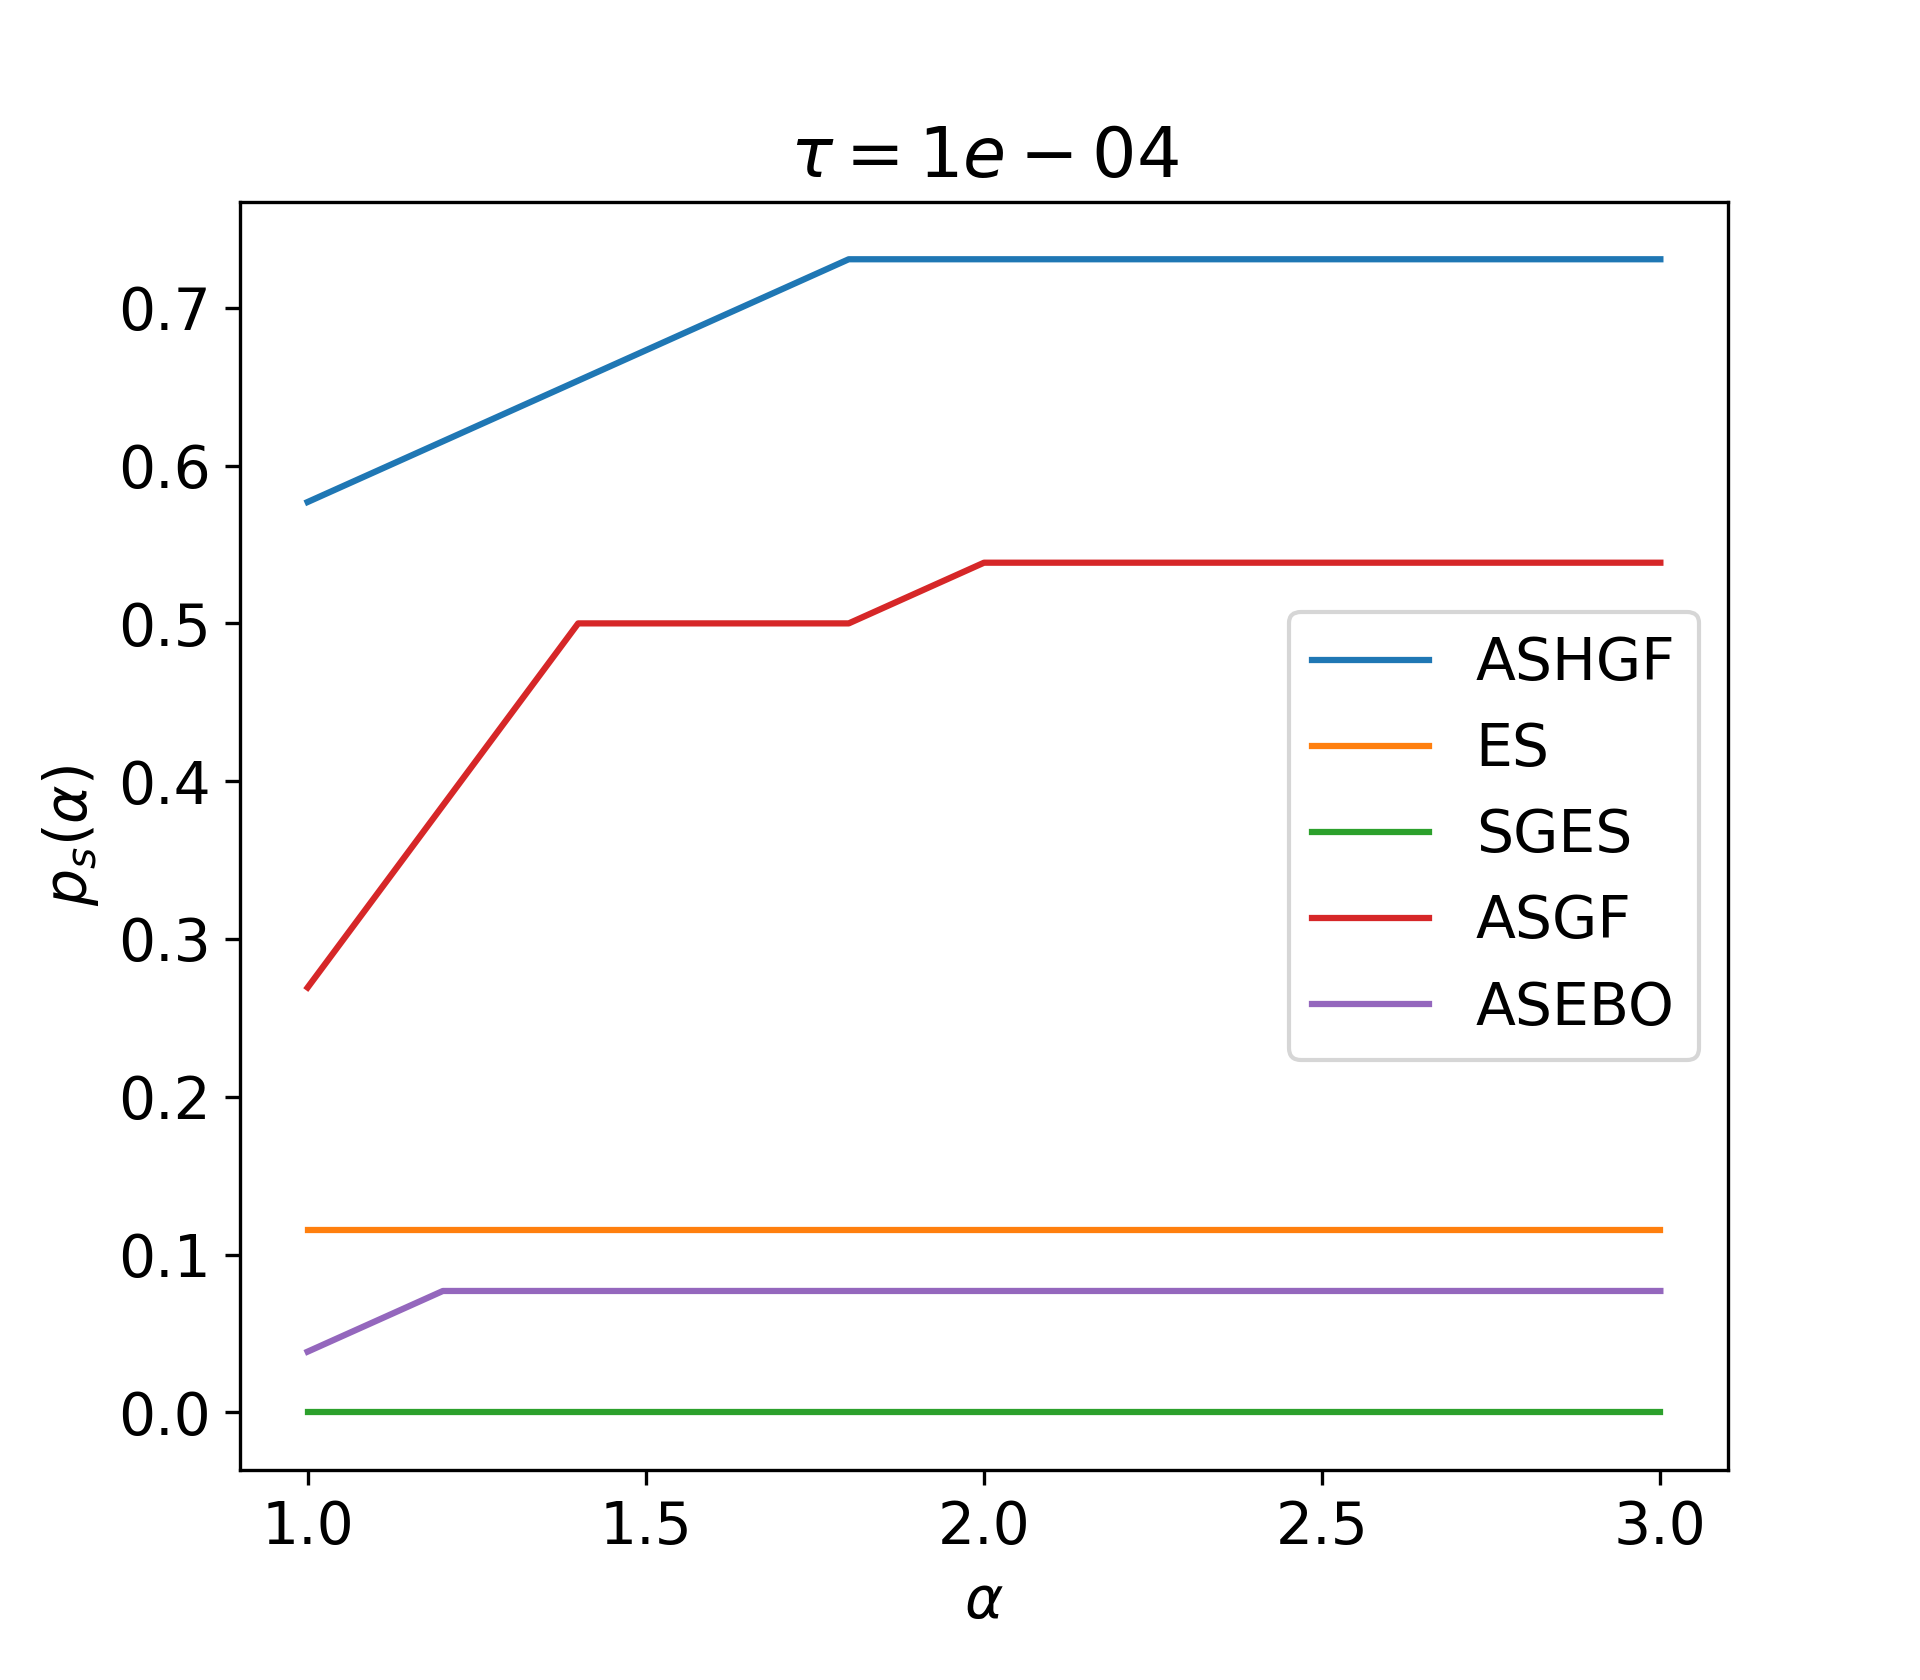
\includegraphics[width=1\textwidth]{figures/performance_profiles/10/performance_profile_10_1000000_1e-04.png}
\end{subfigure}
\begin{subfigure}{0.3\textwidth}
  \centering 
  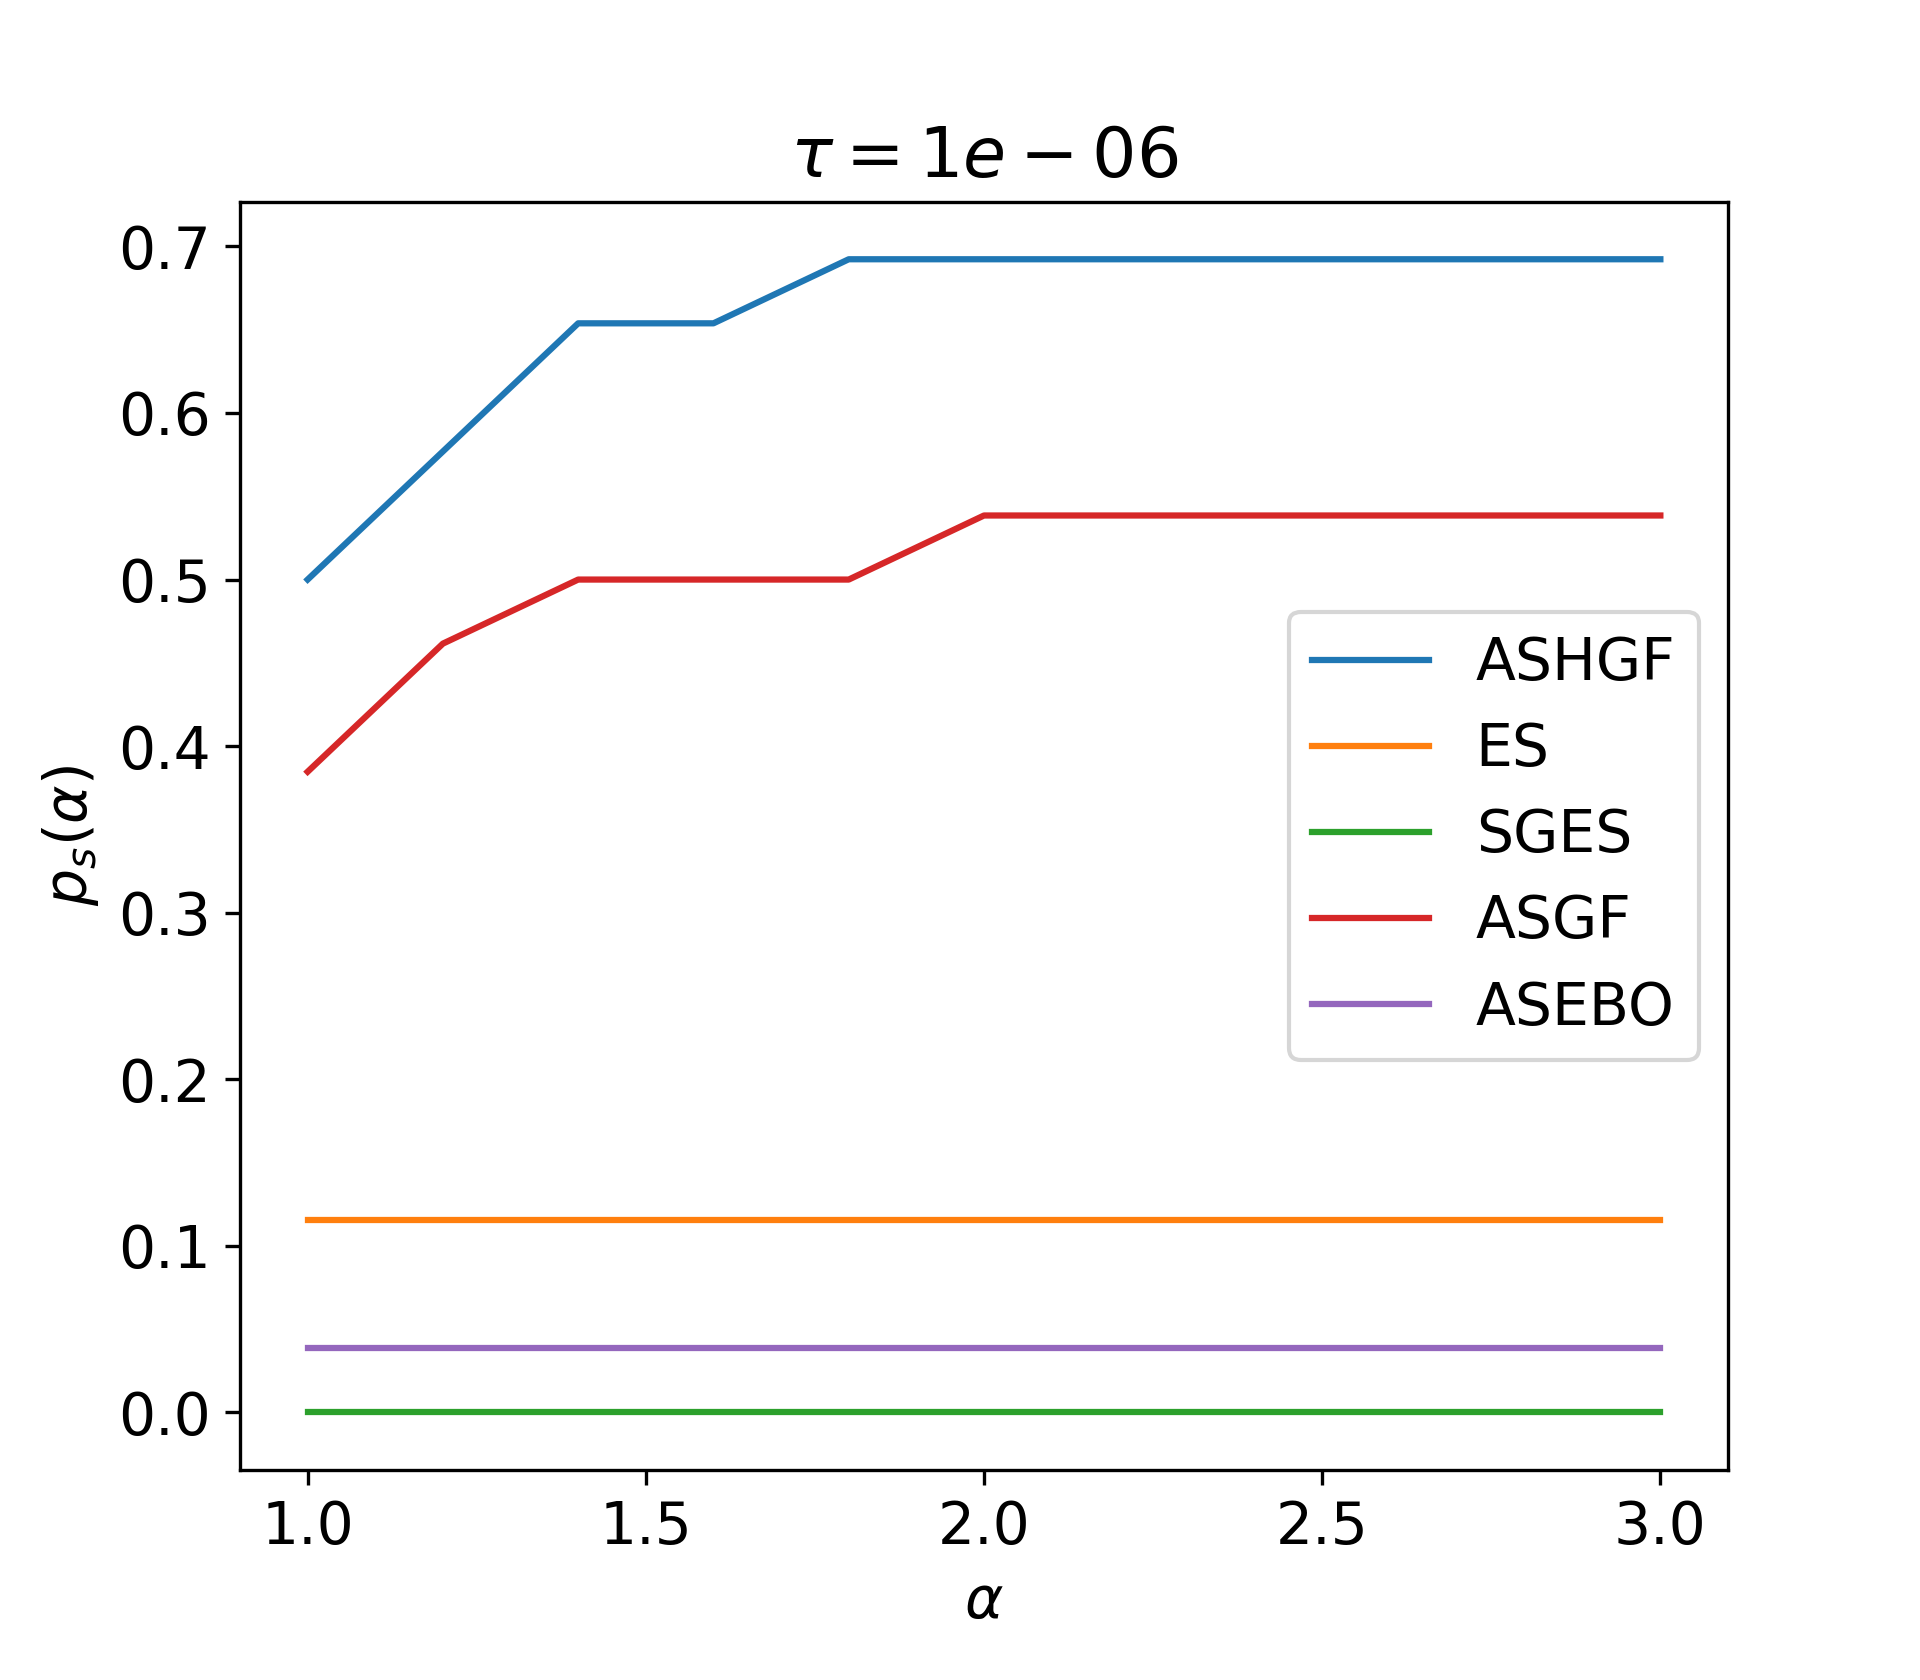
\includegraphics[width=1\textwidth]{figures/performance_profiles/10/performance_profile_10_1000000_1e-06.png}
\end{subfigure}
\centering
\begin{subfigure}{0.3\textwidth}
  \centering 
  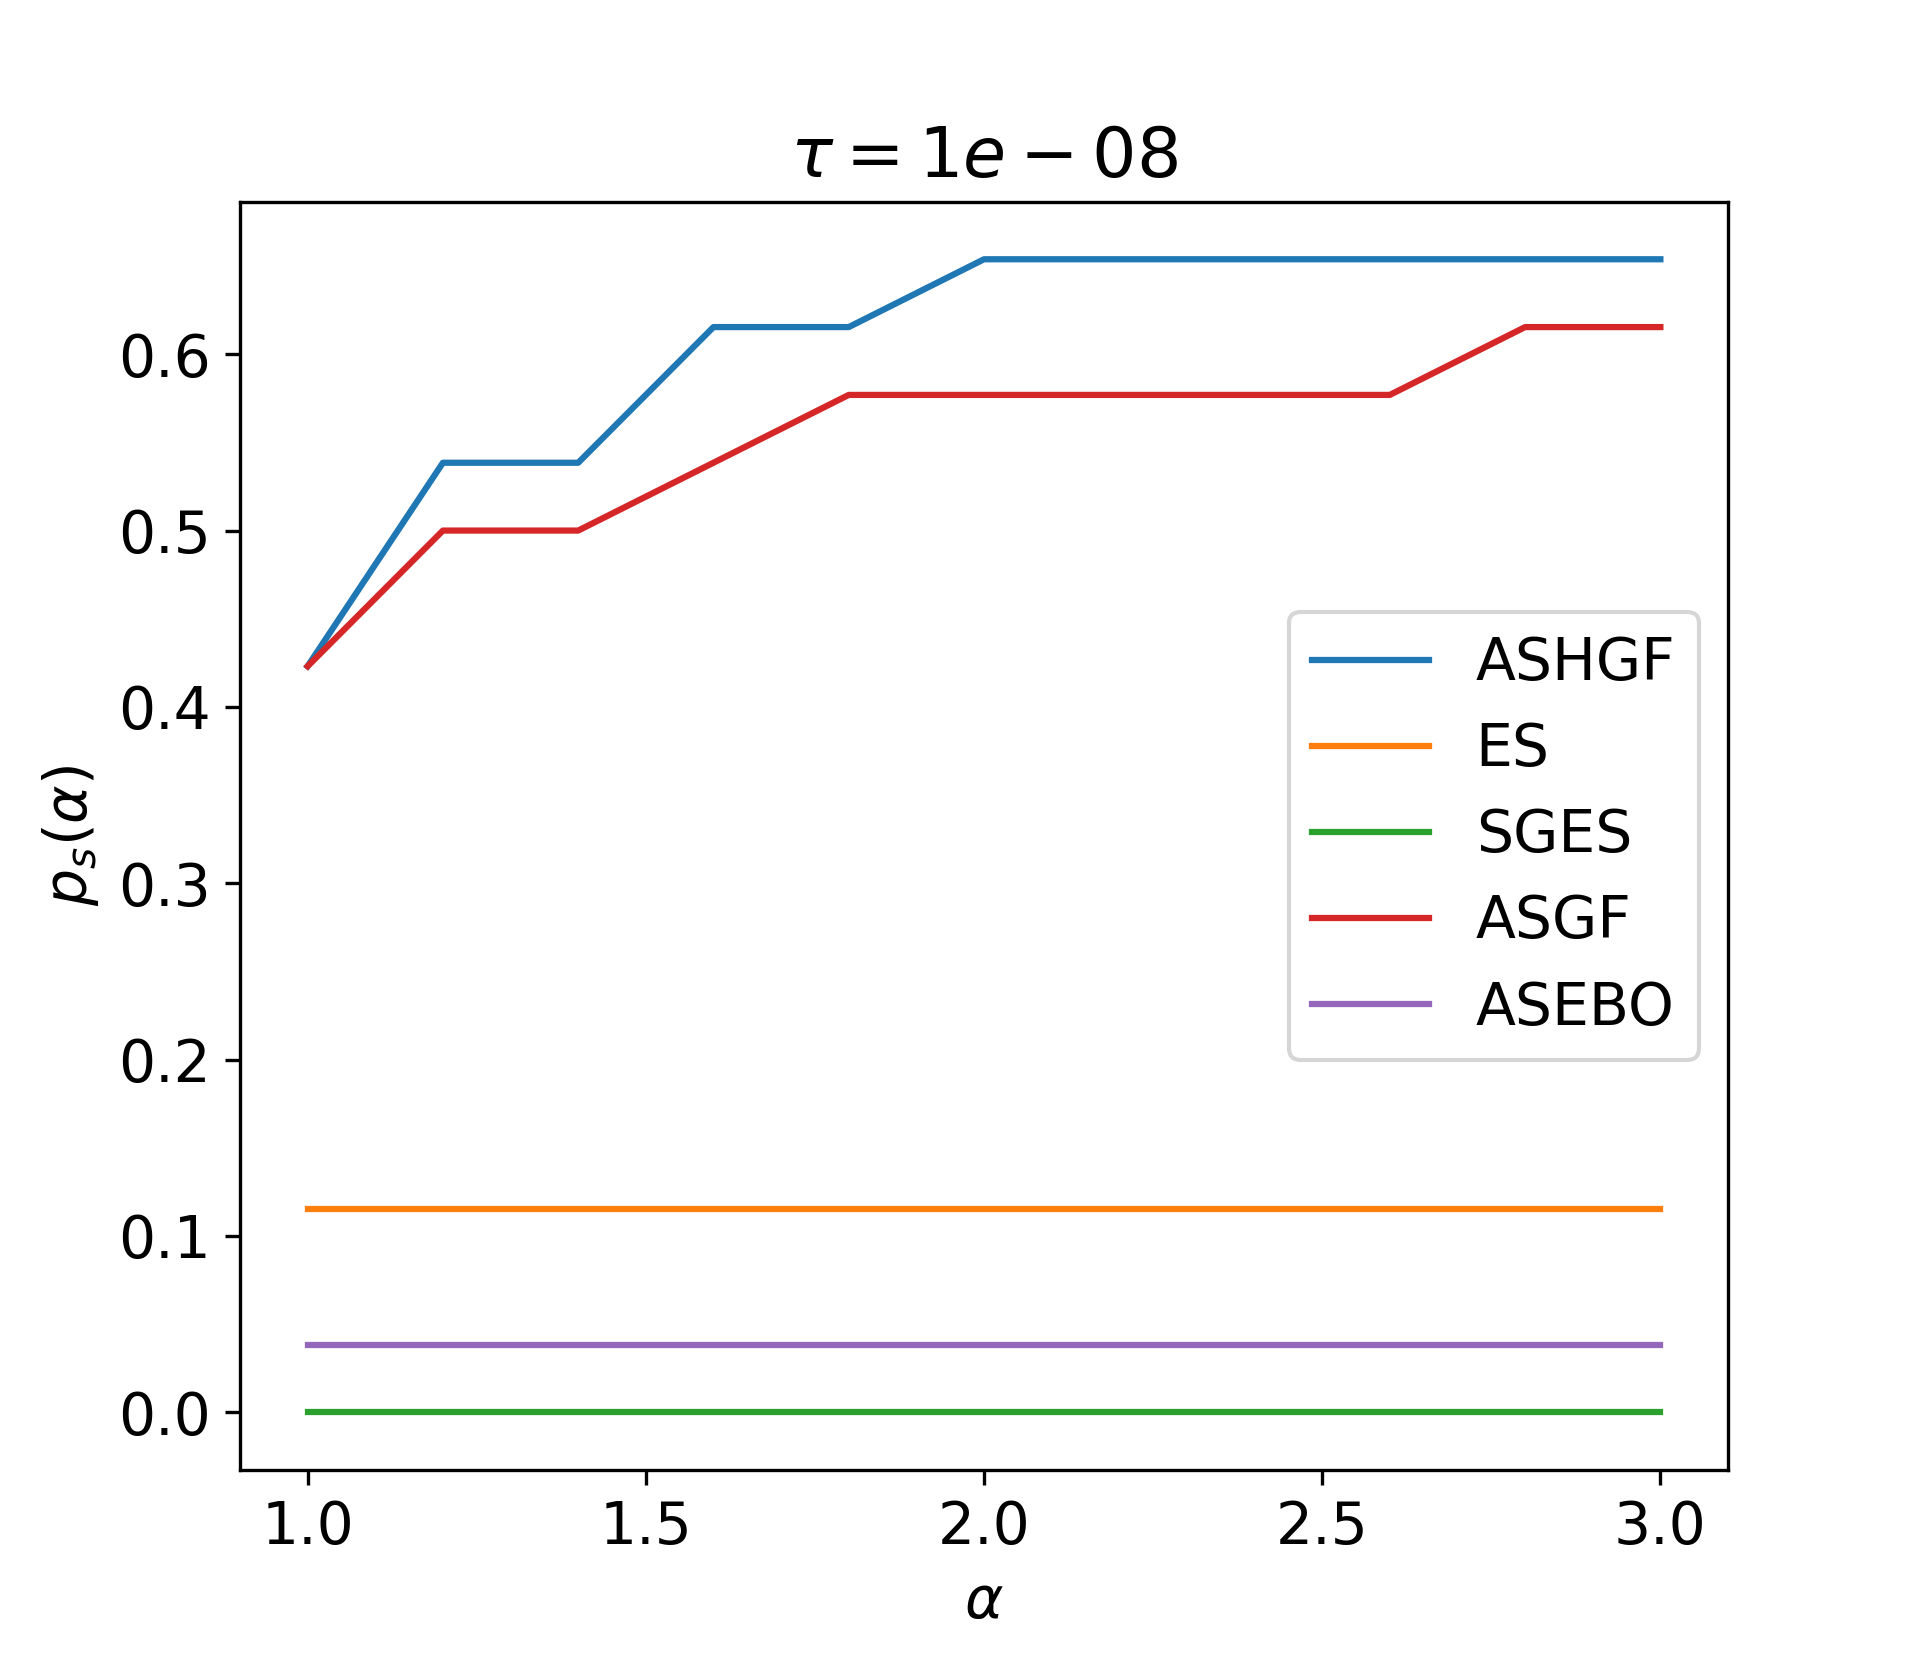
\includegraphics[width=1\textwidth]{figures/performance_profiles/10/performance_profile_10_1000000_1e-08.png}
\end{subfigure}%
\begin{subfigure}{0.3\textwidth}
  \centering 
  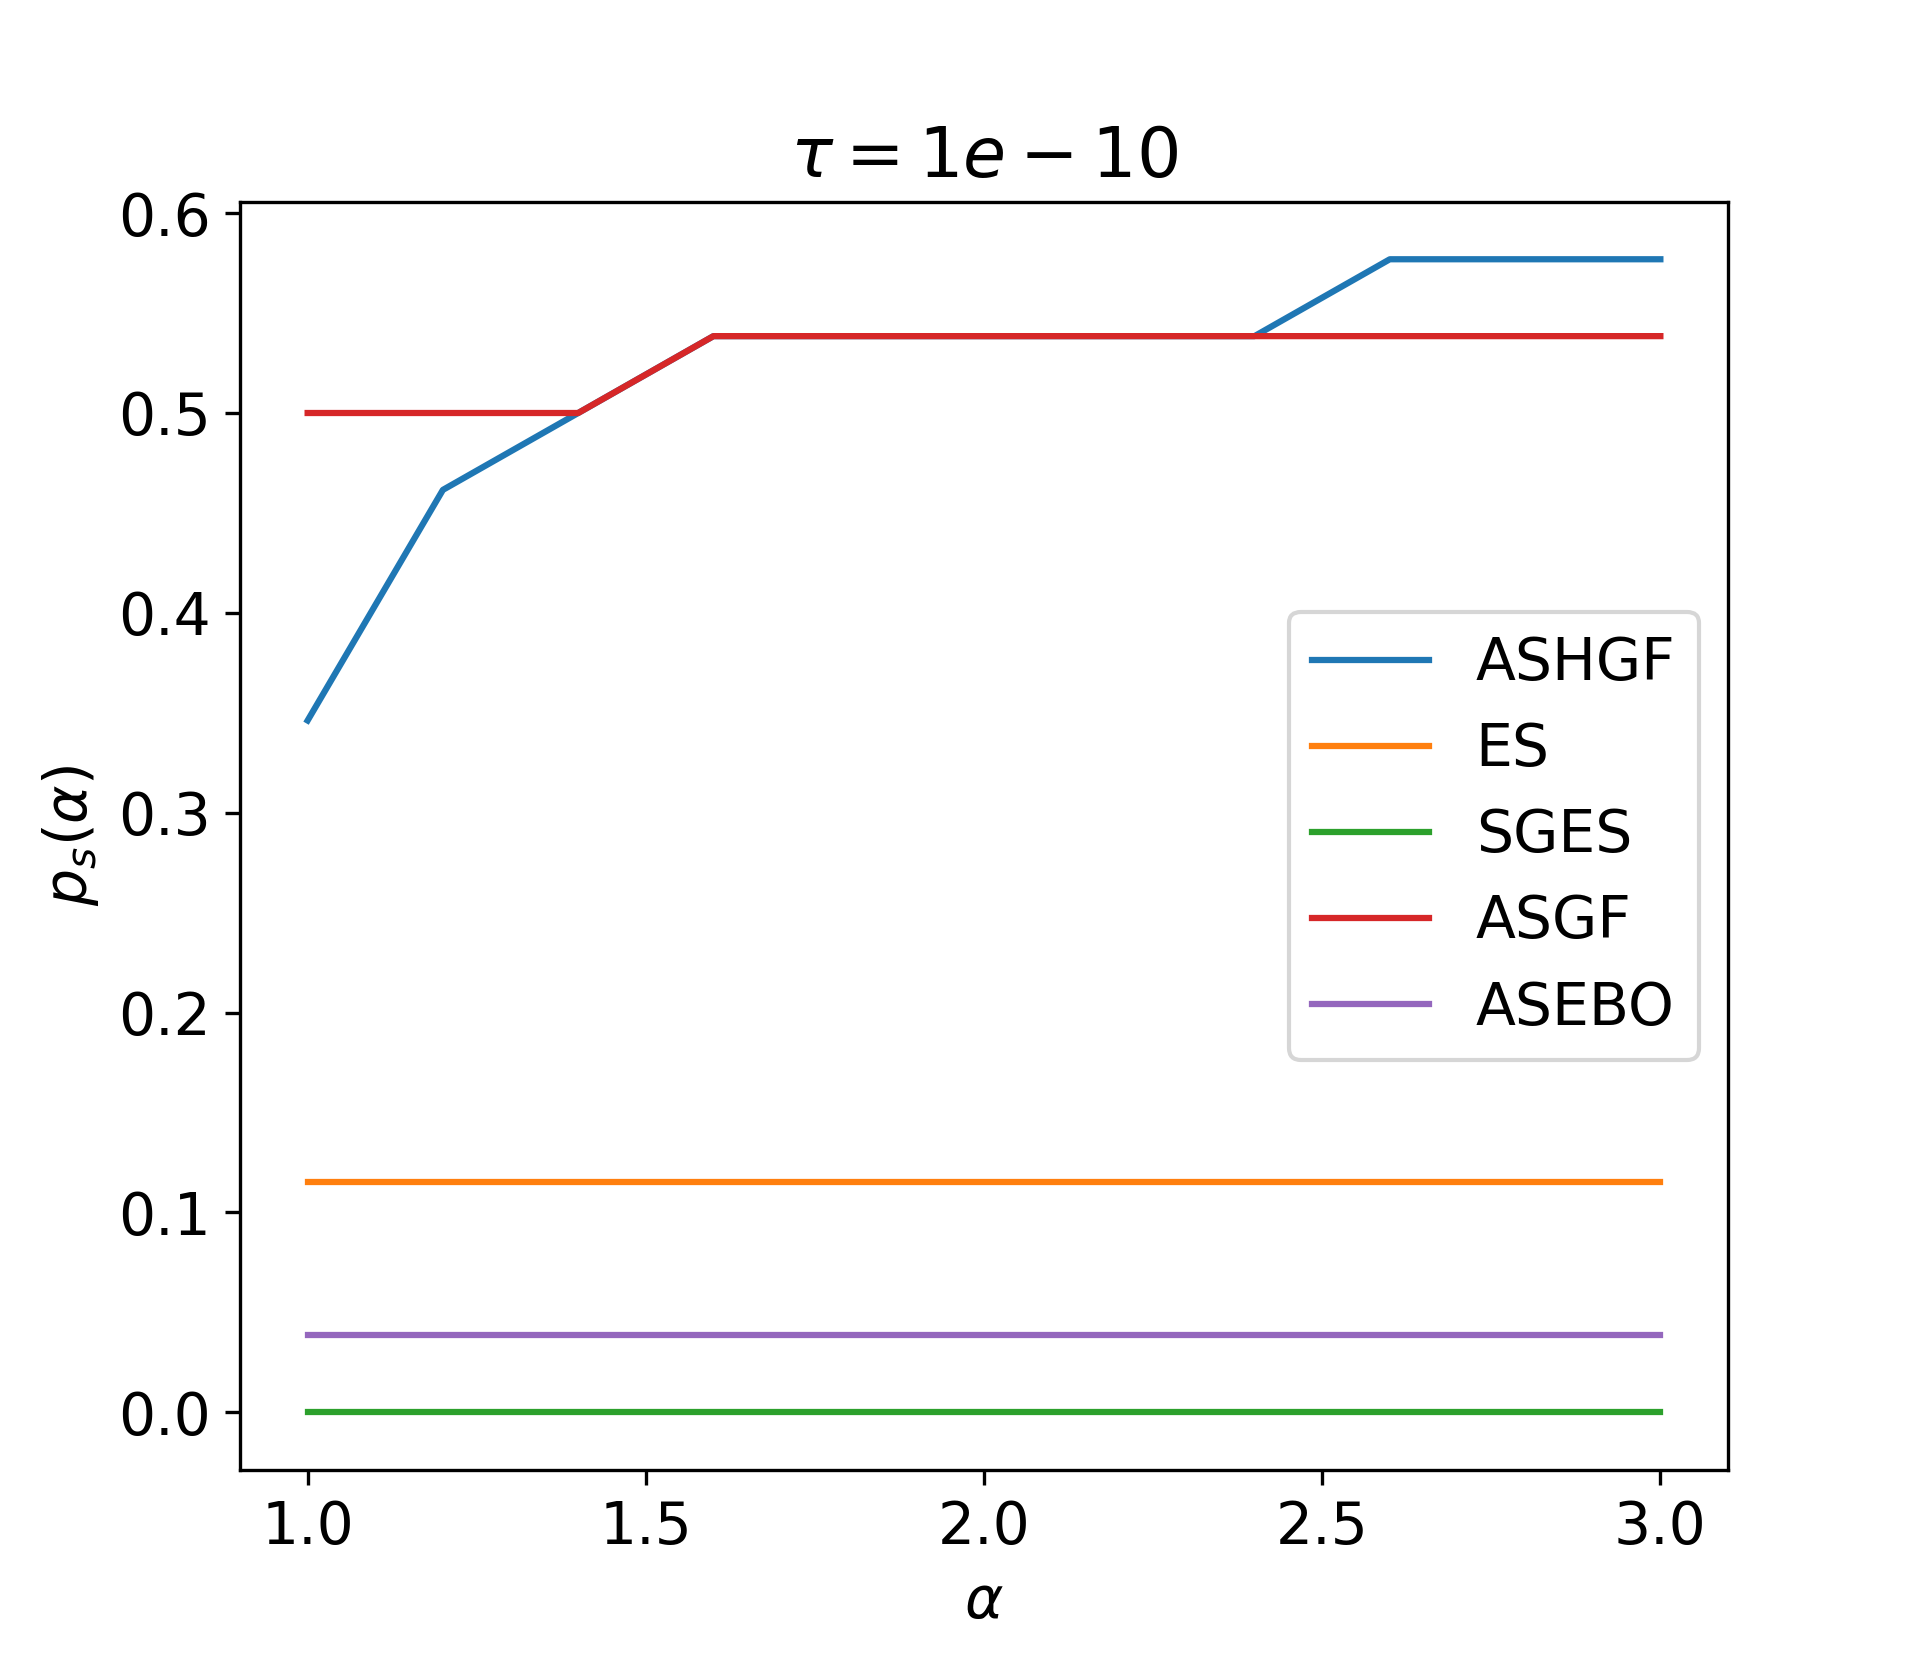
\includegraphics[width=1\textwidth]{figures/performance_profiles/10/performance_profile_10_1000000_1e-10.png}
\end{subfigure}
\caption{Performance profiles with $\mu_L = 10^{6}$}
\label{PerformanceProfiles10Mu1000000}
\end{figure}

\begin{figure}[H]
\centering
\begin{subfigure}{0.3\textwidth}
  \centering 
  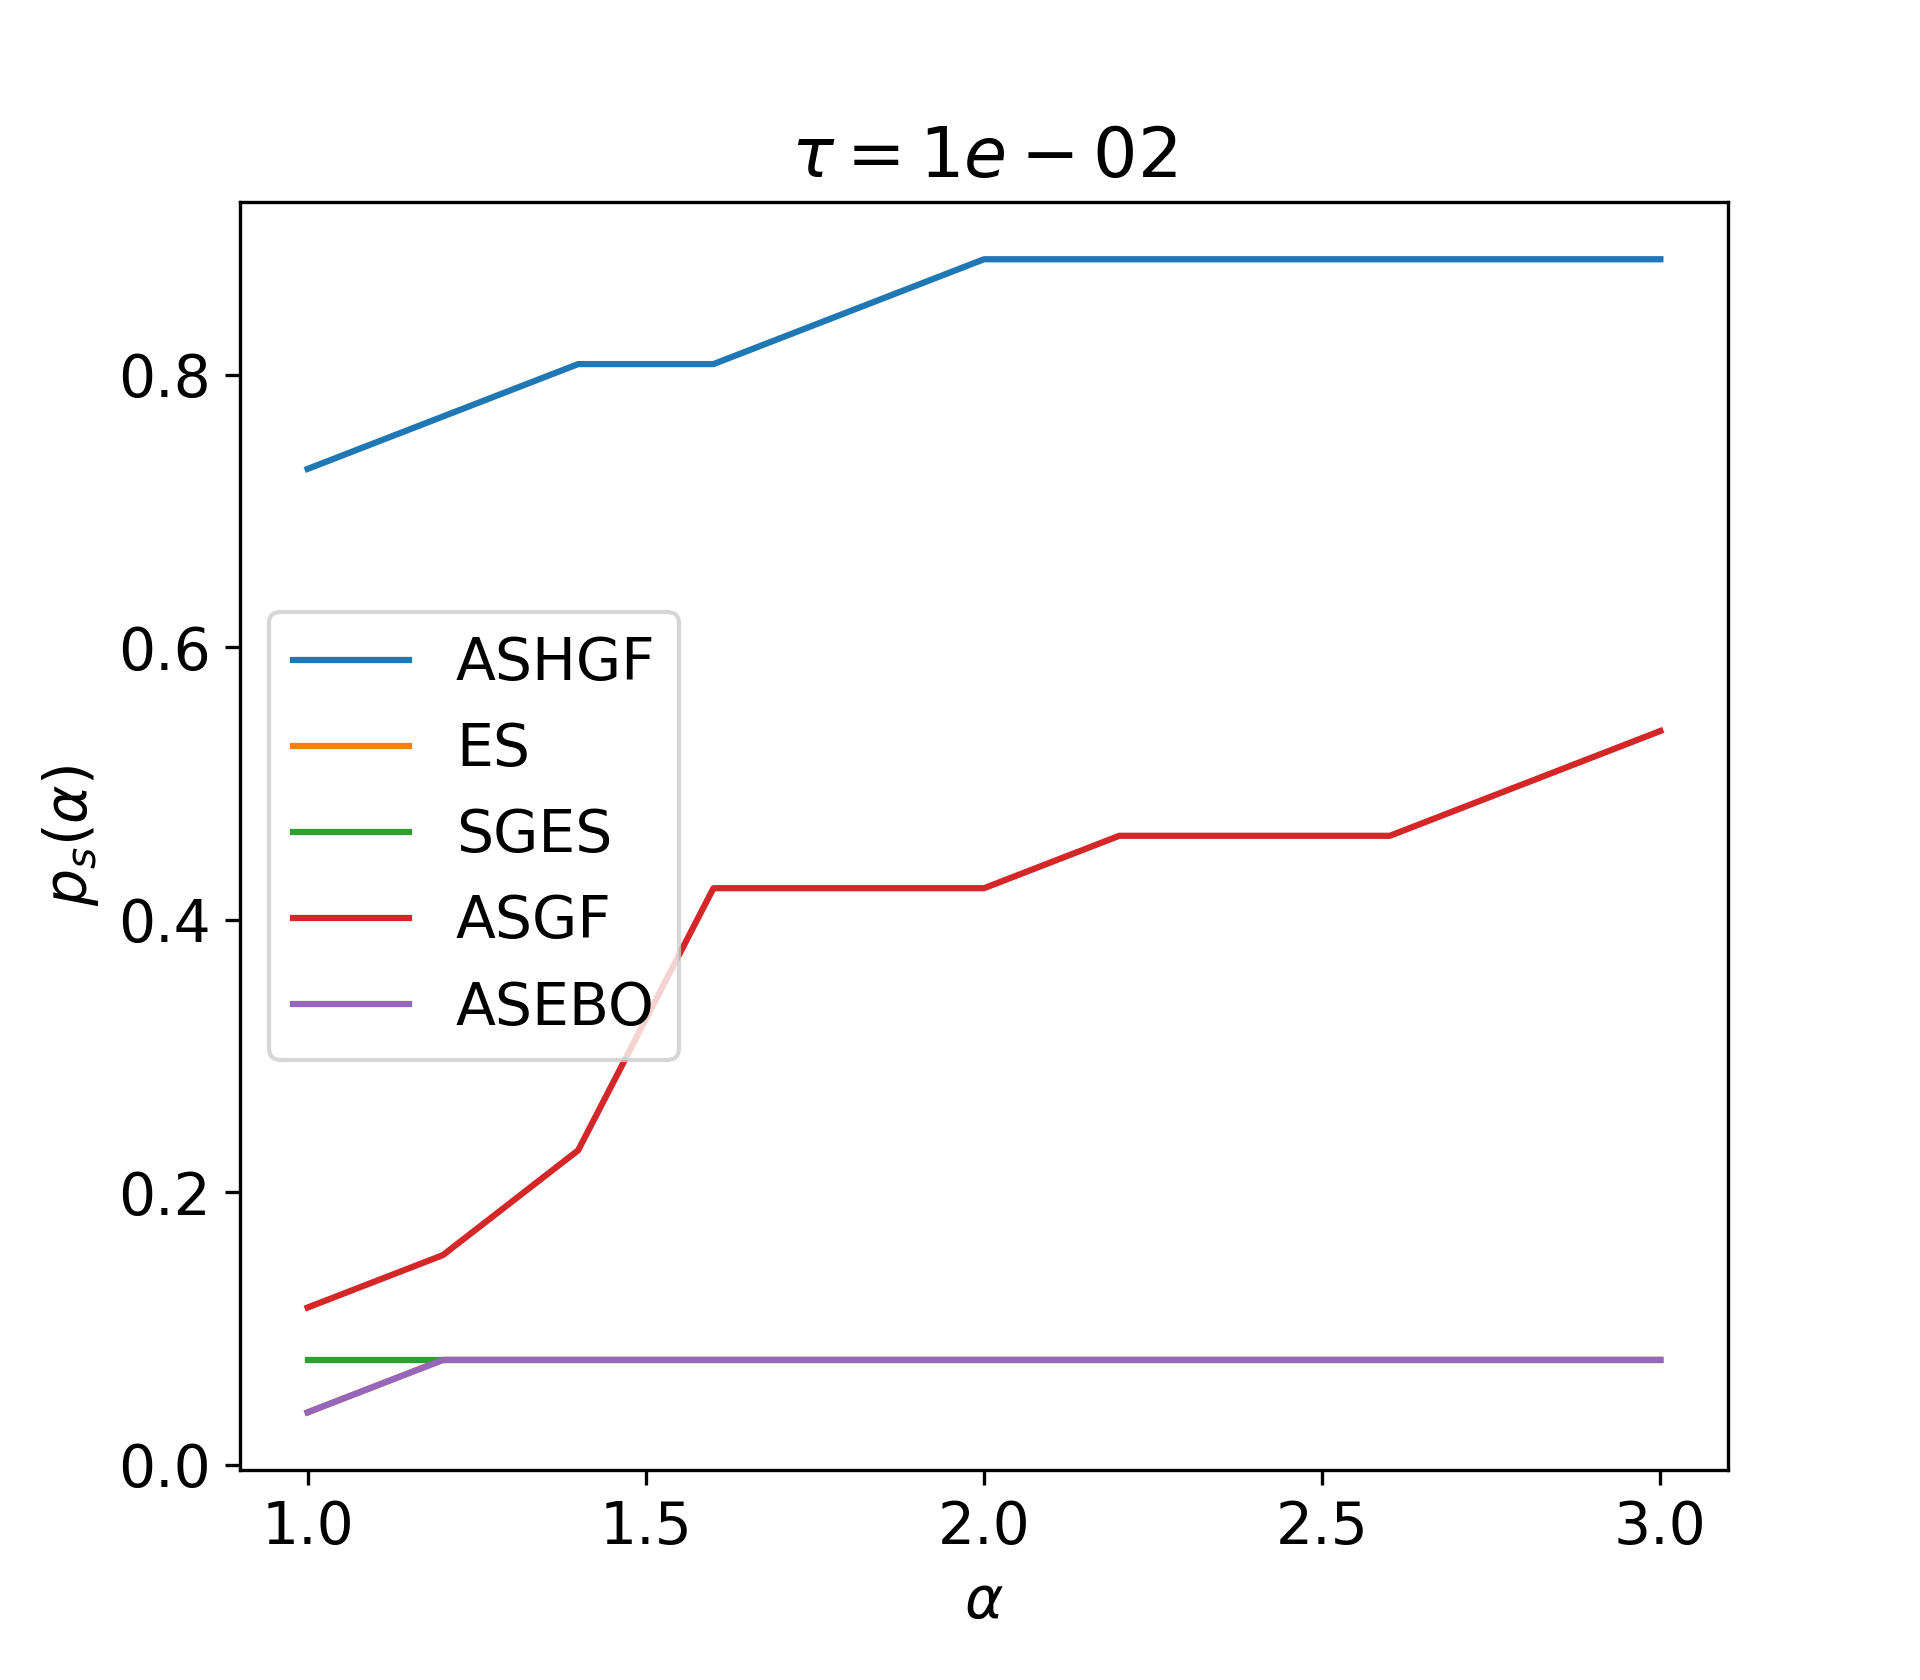
\includegraphics[width=1\textwidth]{figures/performance_profiles/10/performance_profile_10_10000000_1e-02.png}
\end{subfigure}%
\begin{subfigure}{0.3\textwidth}
  \centering 
  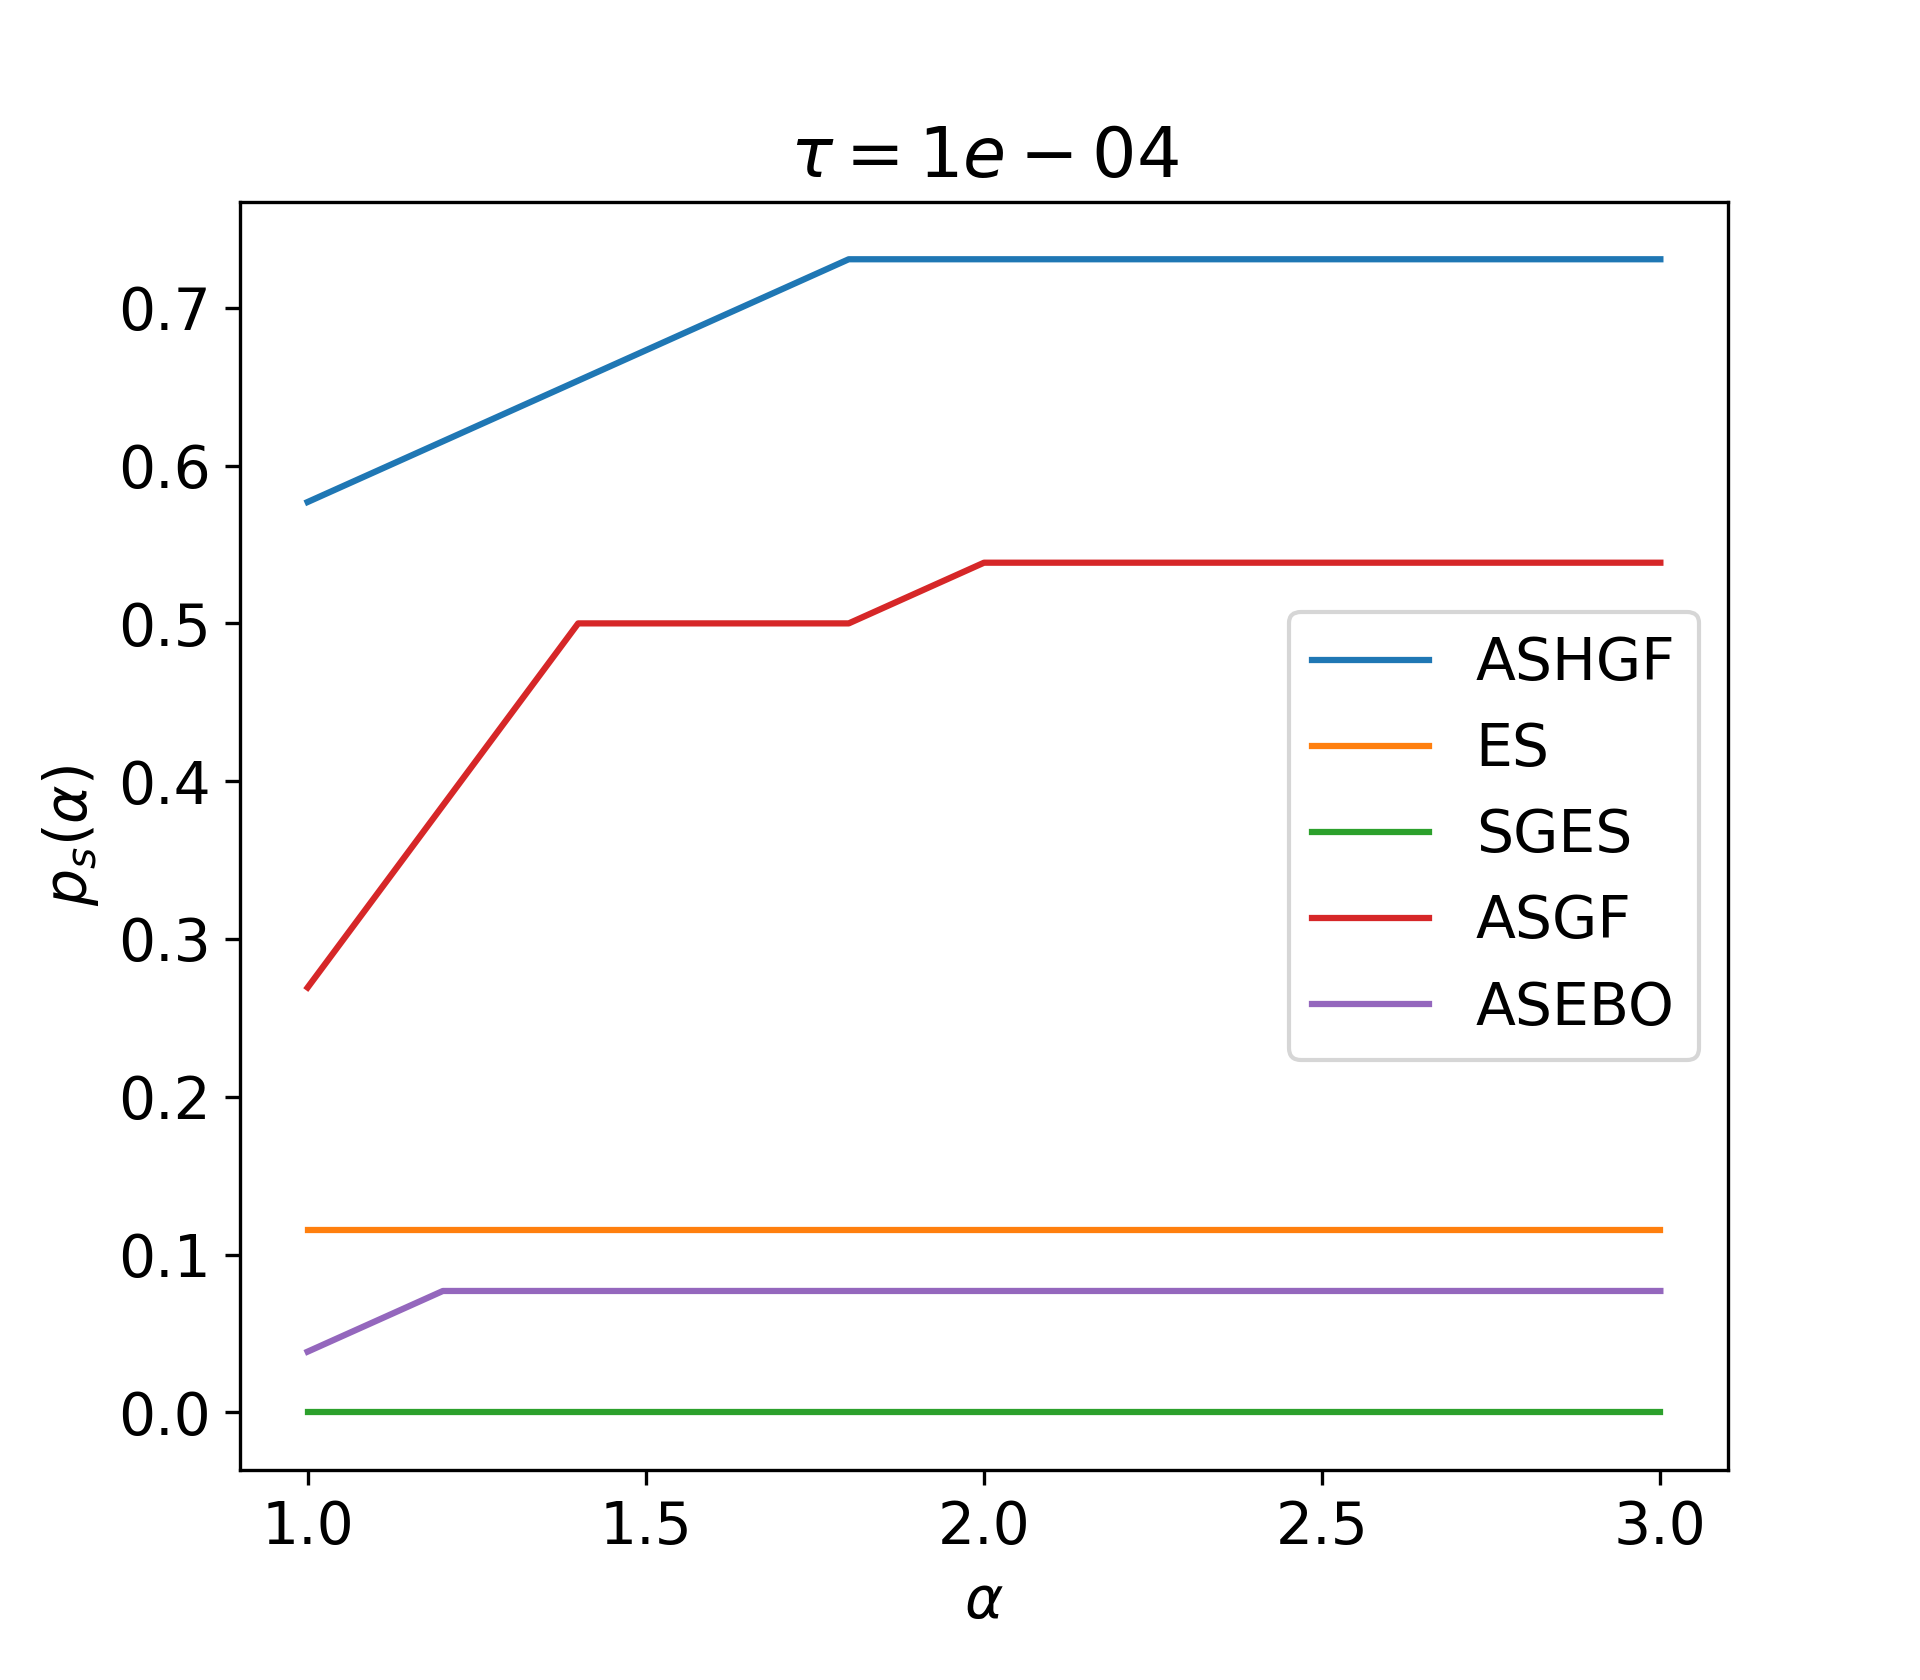
\includegraphics[width=1\textwidth]{figures/performance_profiles/10/performance_profile_10_10000000_1e-04.png}
\end{subfigure}
\begin{subfigure}{0.3\textwidth}
  \centering 
  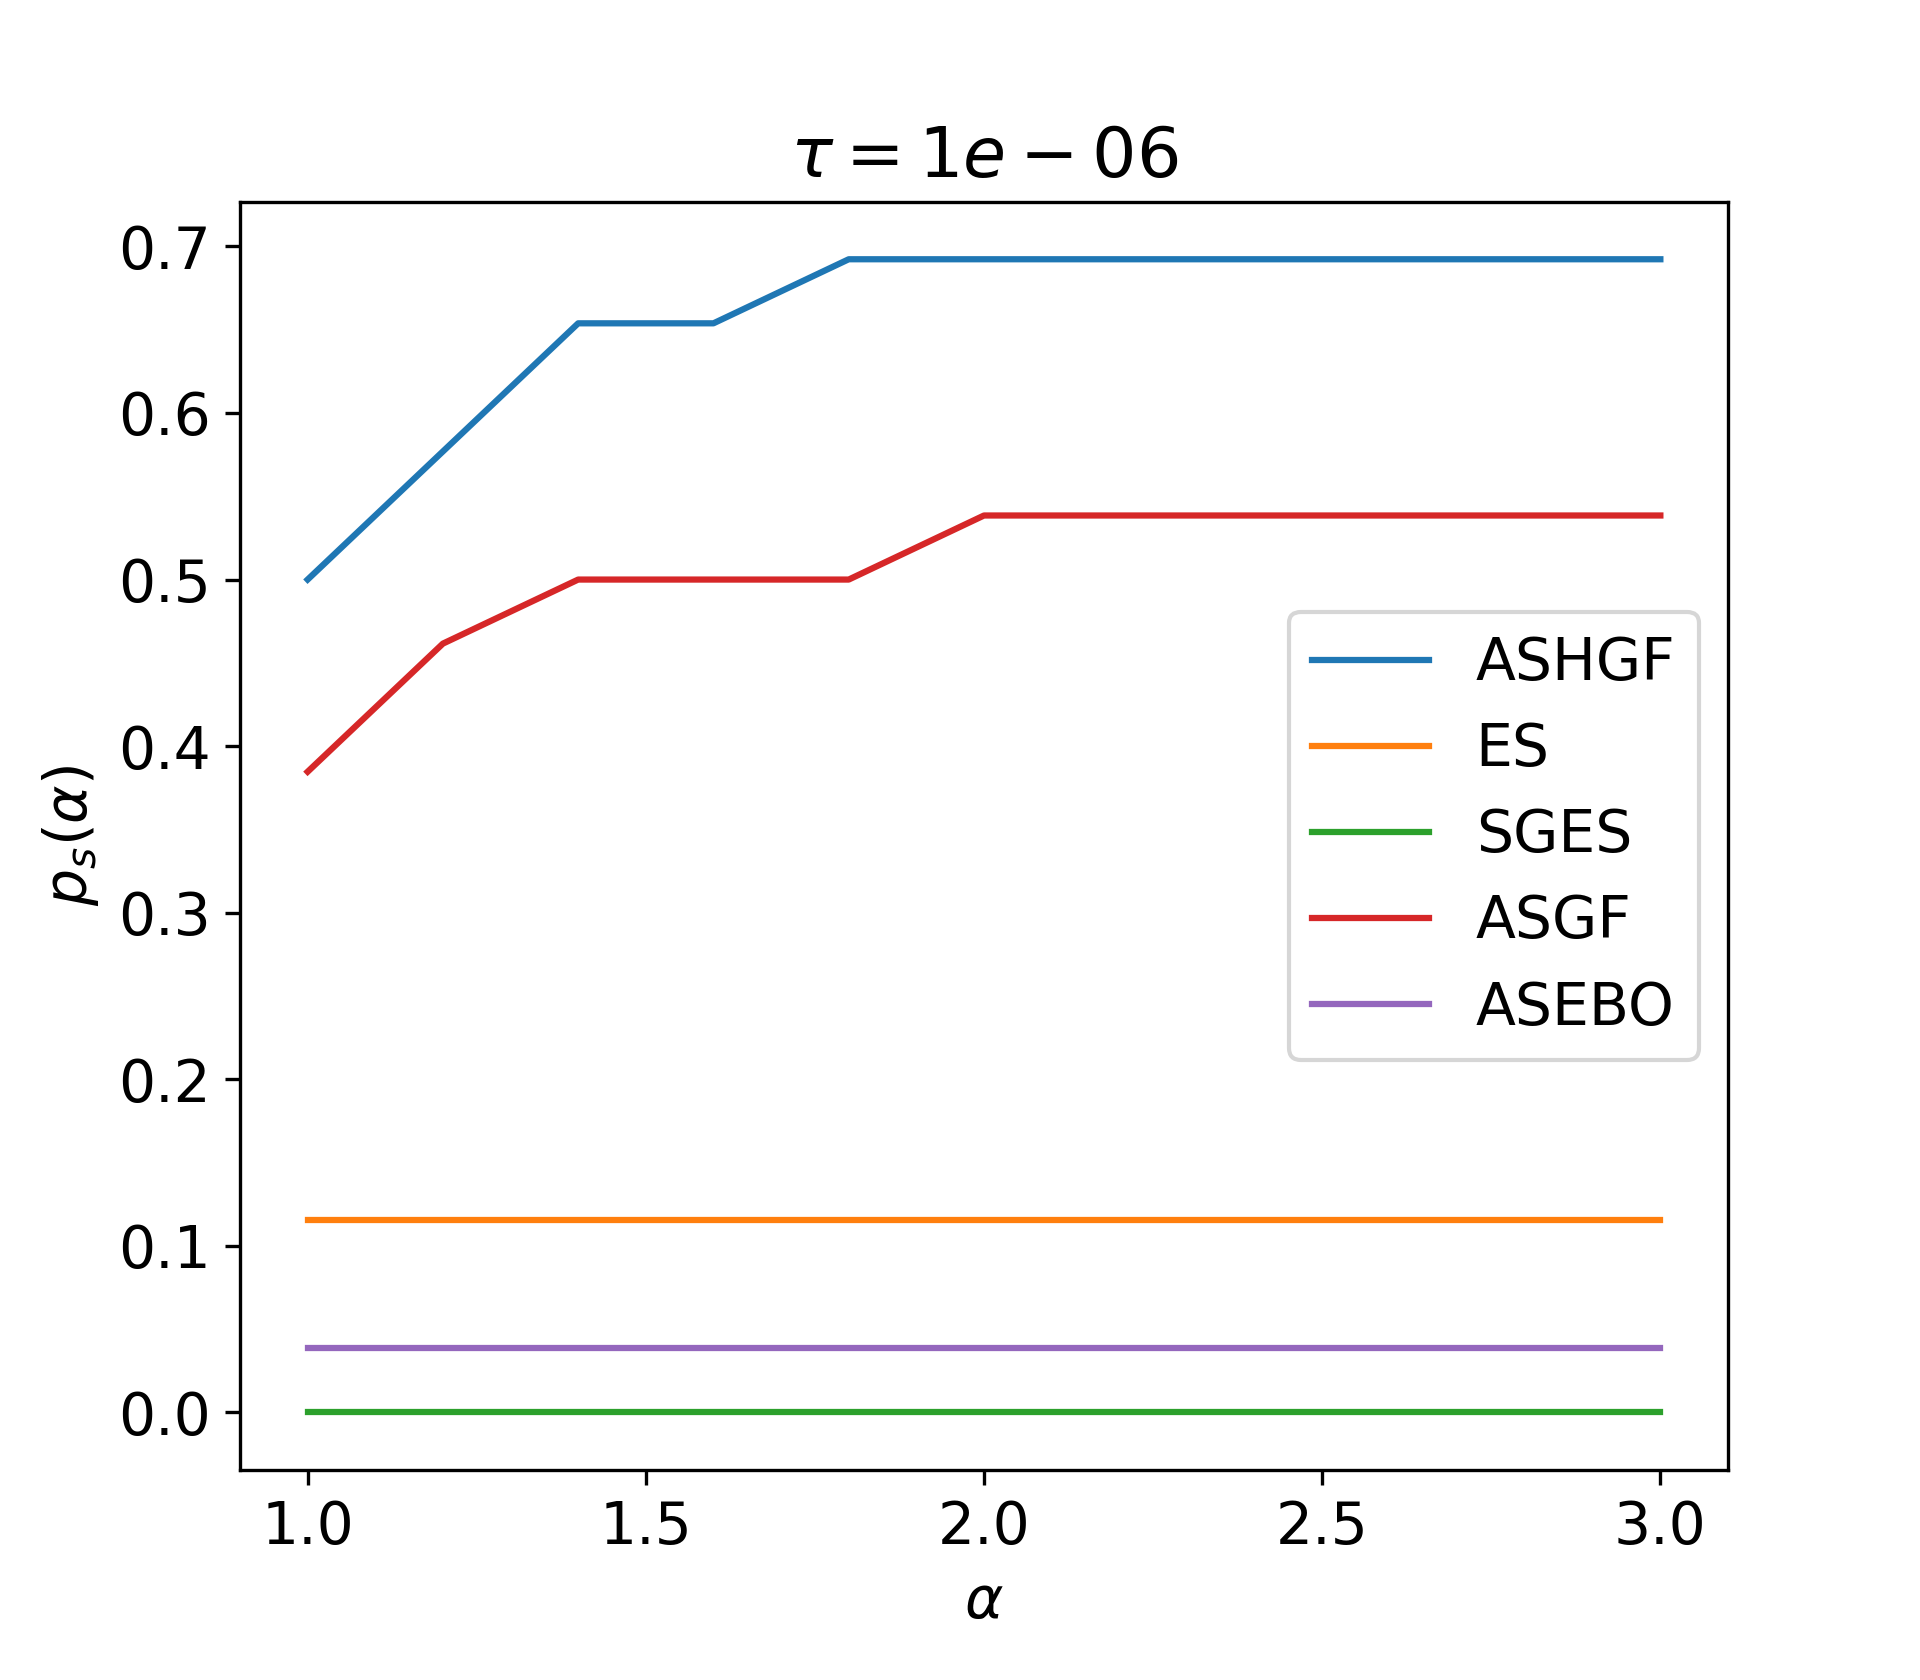
\includegraphics[width=1\textwidth]{figures/performance_profiles/10/performance_profile_10_10000000_1e-06.png}
\end{subfigure}
\centering
\begin{subfigure}{0.3\textwidth}
  \centering 
  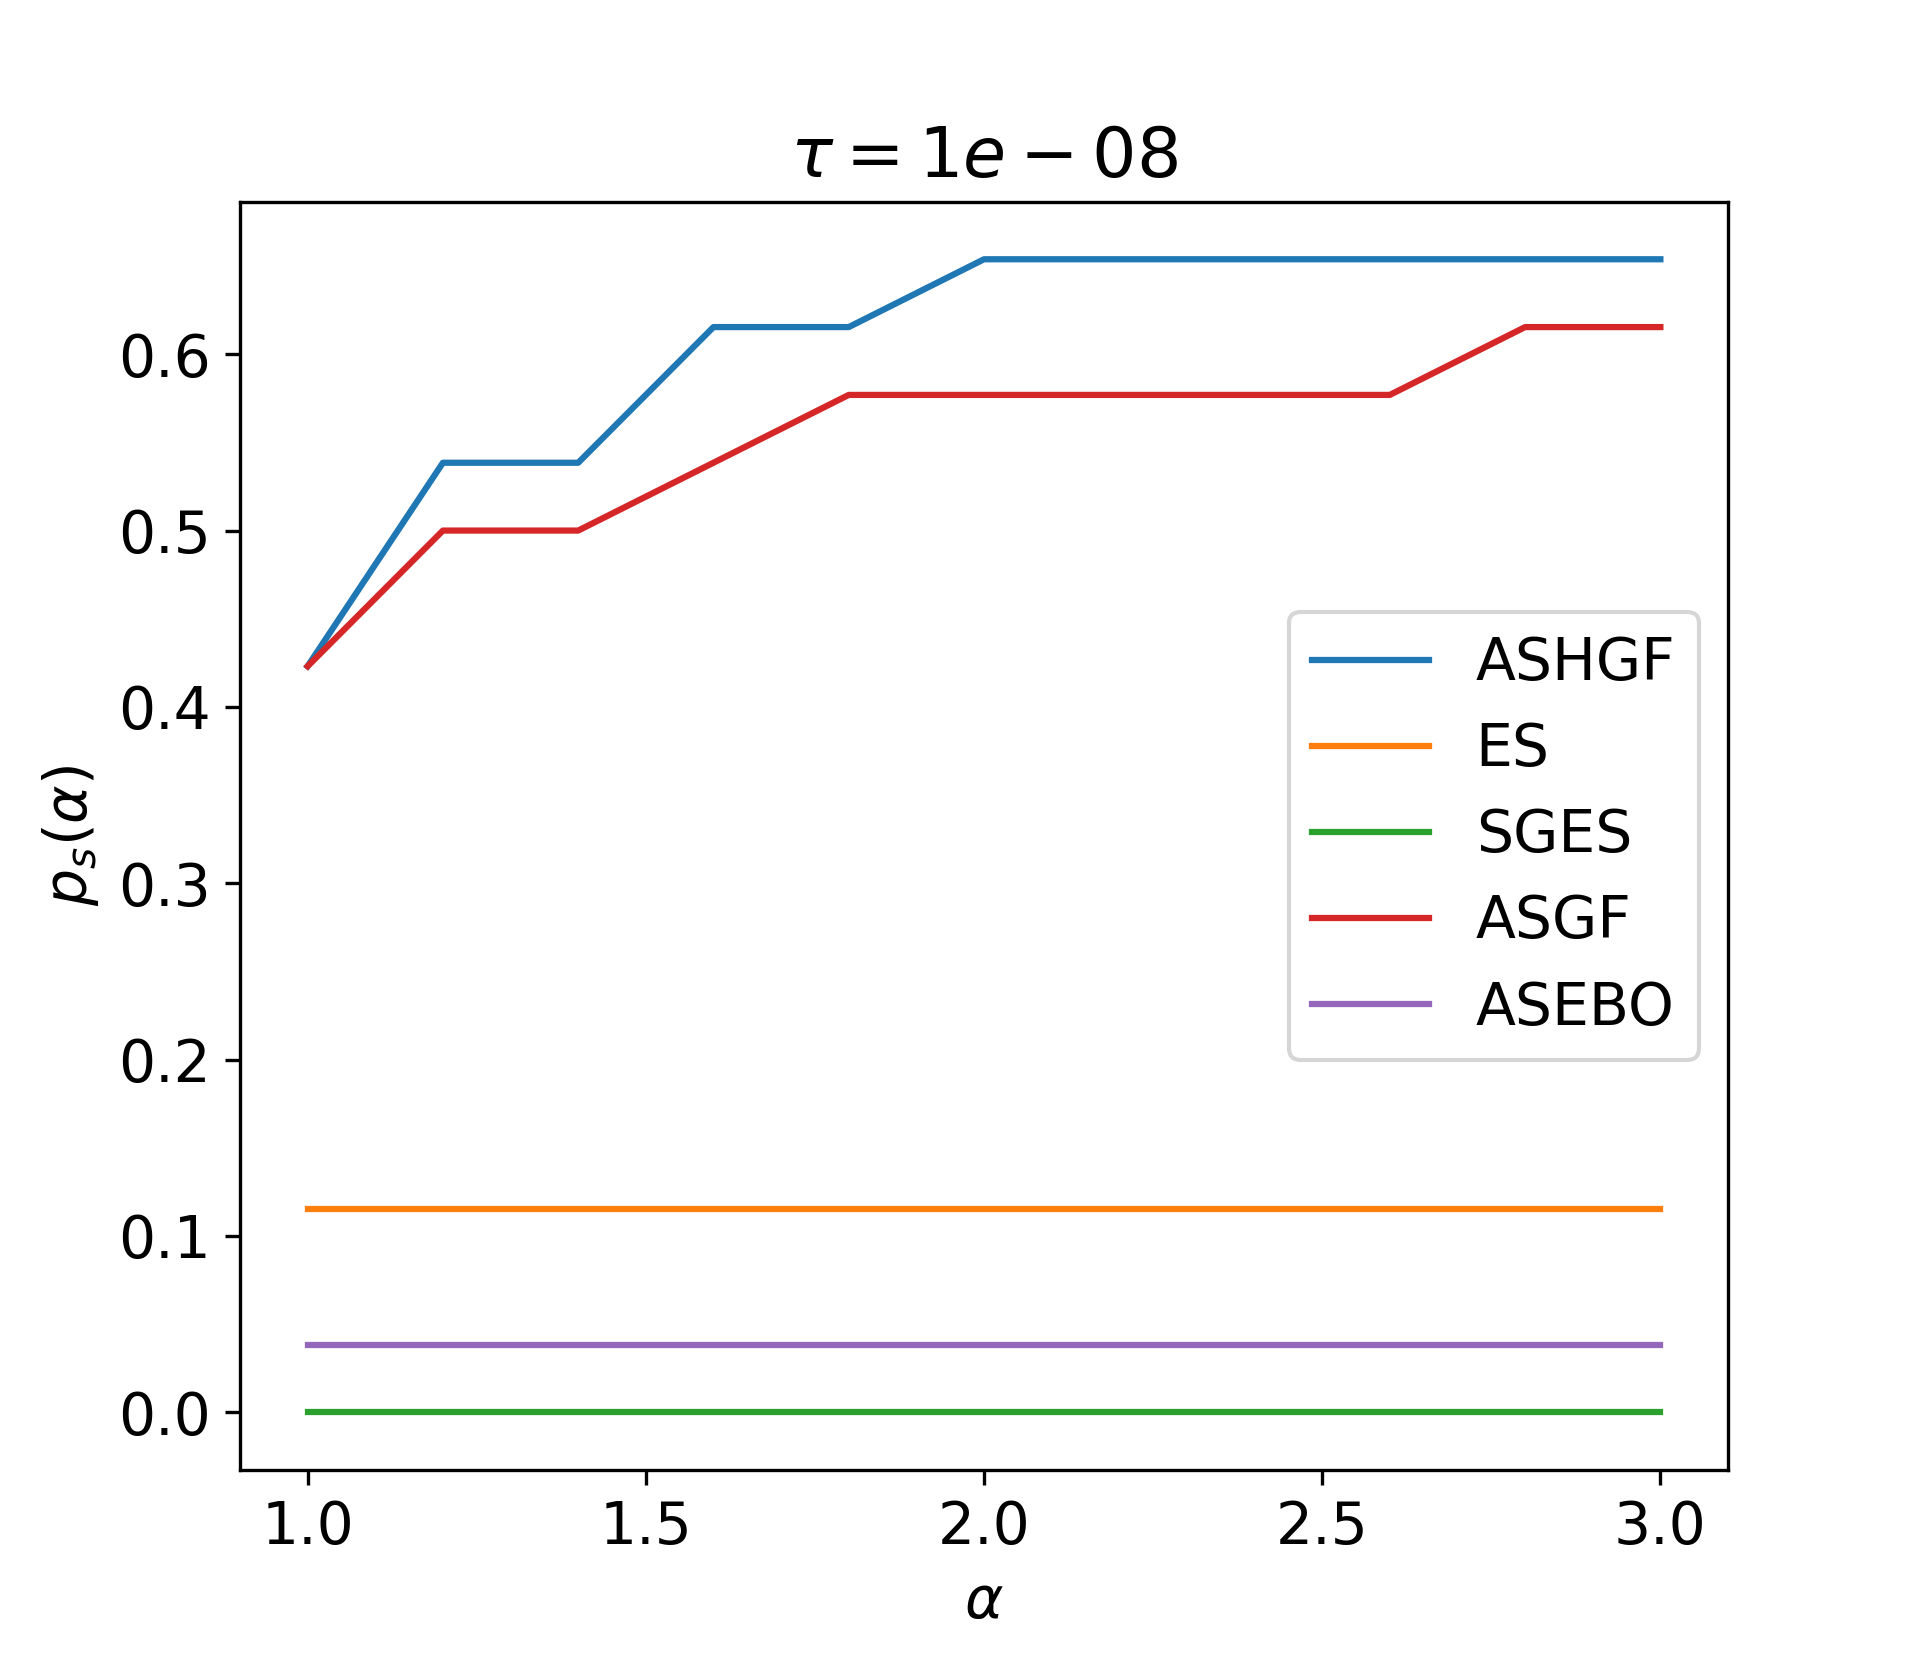
\includegraphics[width=1\textwidth]{figures/performance_profiles/10/performance_profile_10_10000000_1e-08.png}
\end{subfigure}%
\begin{subfigure}{0.3\textwidth}
  \centering 
  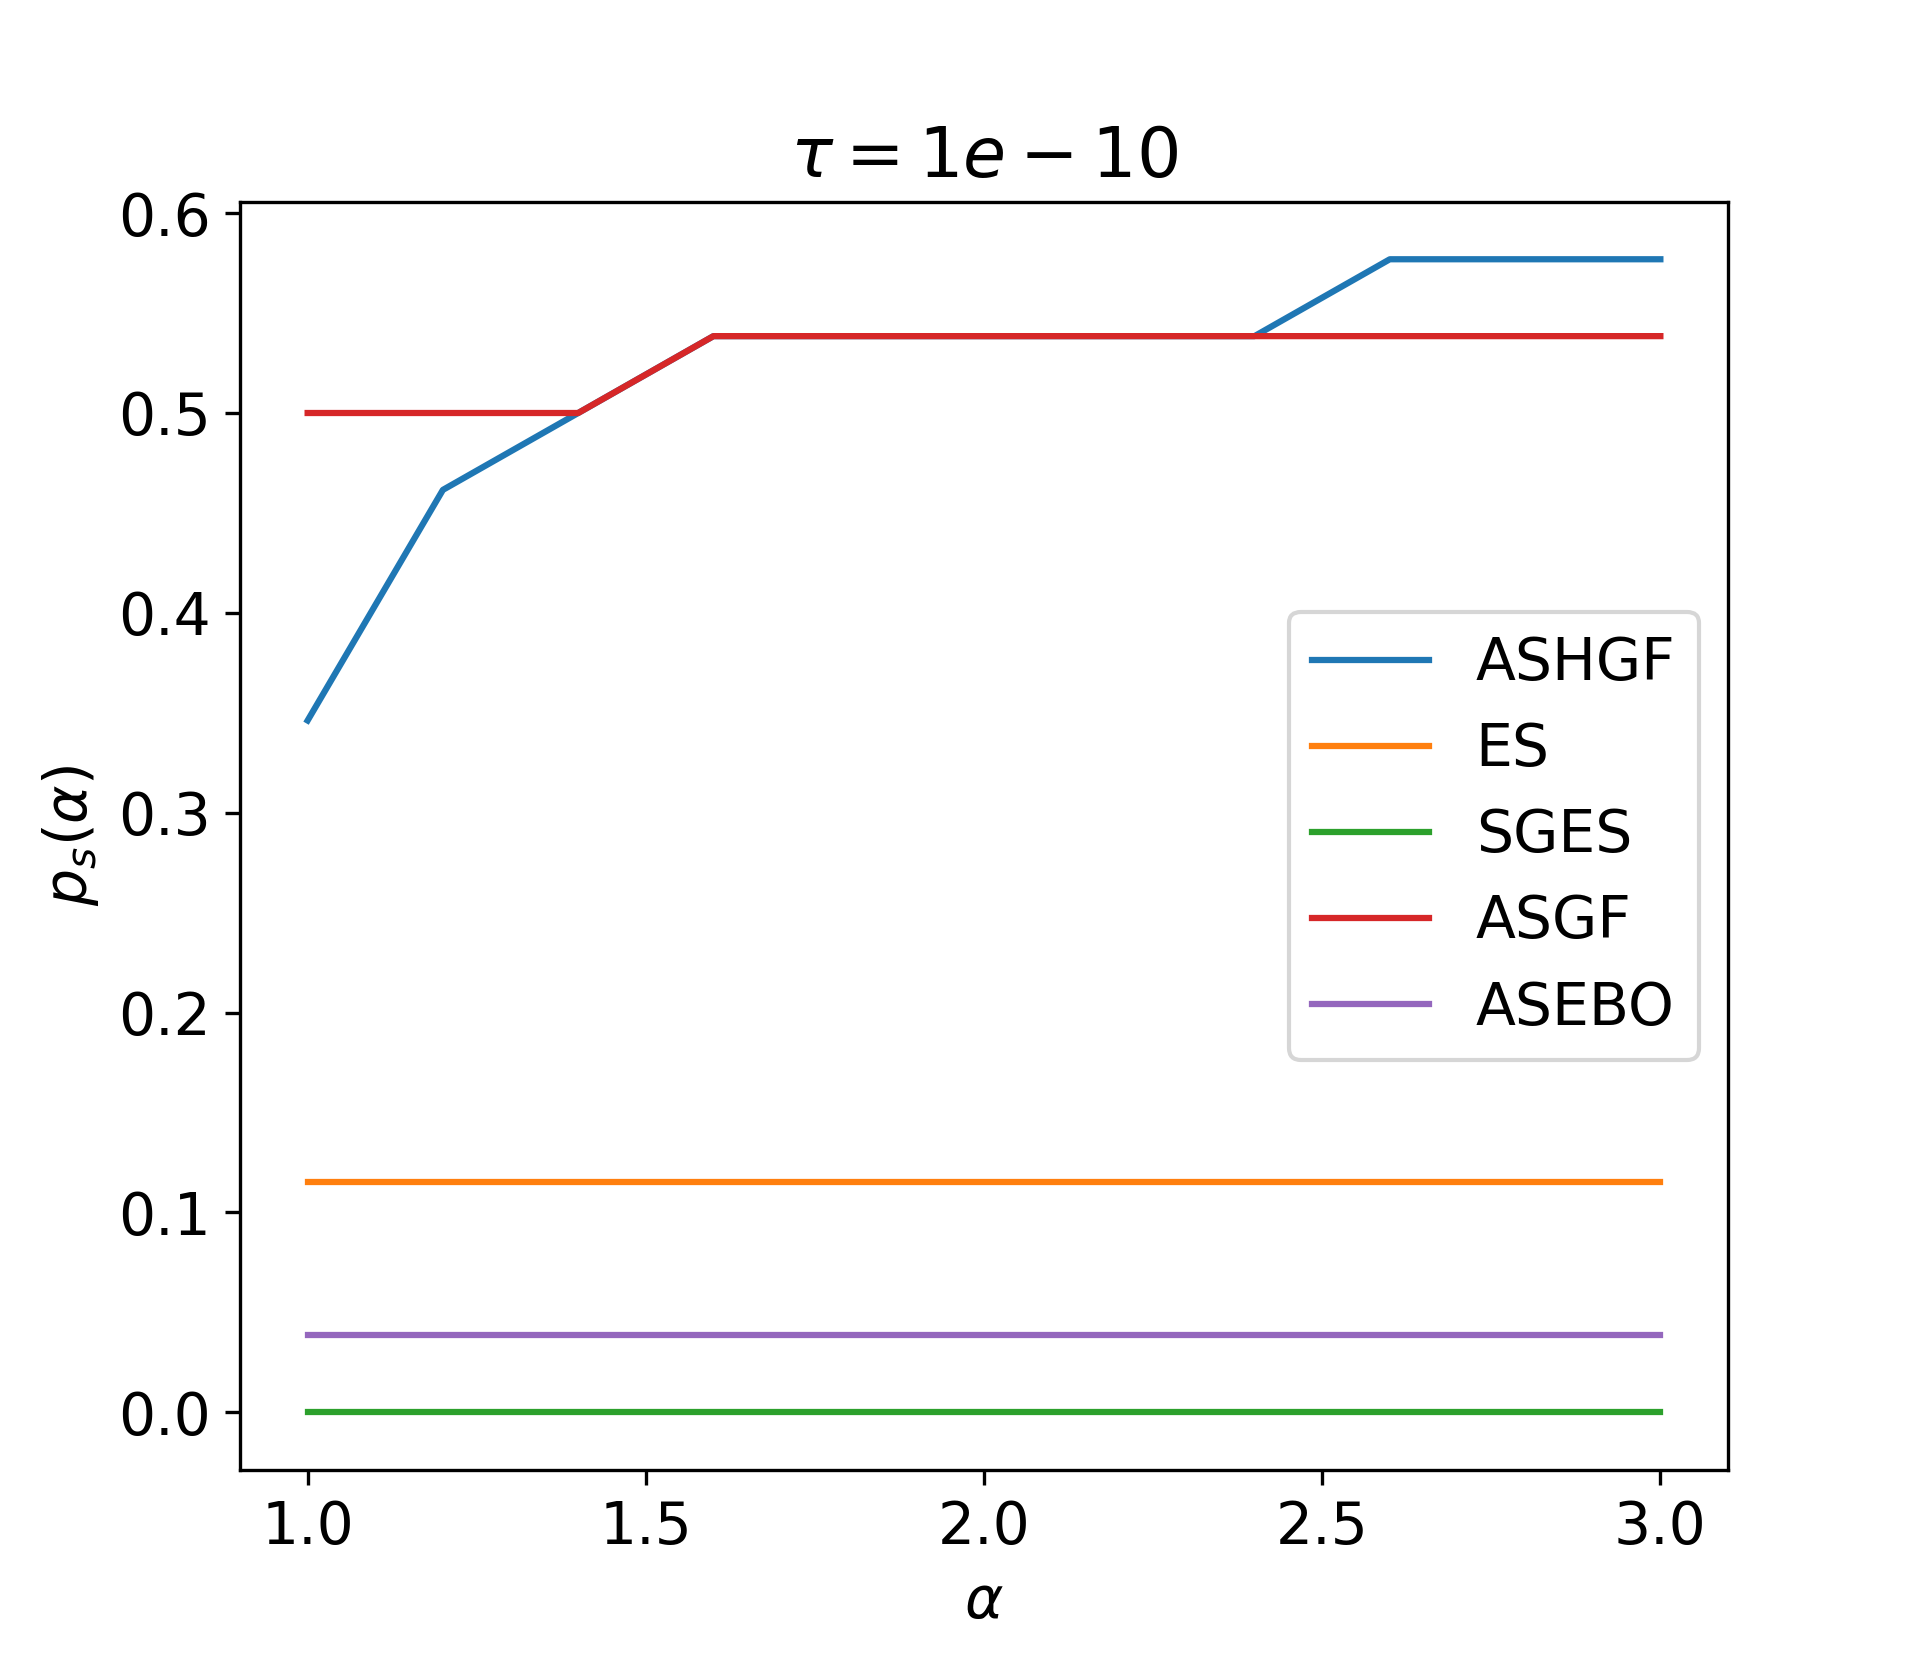
\includegraphics[width=1\textwidth]{figures/performance_profiles/10/performance_profile_10_10000000_1e-10.png}
\end{subfigure}
\caption{Performance profiles with $\mu_L = 10^{7}$}
\label{PerformanceProfiles10Mu10000000}
\end{figure}

\begin{figure}[H]
	\centering
	\begin{subfigure}{0.3\textwidth}
		\centering 
		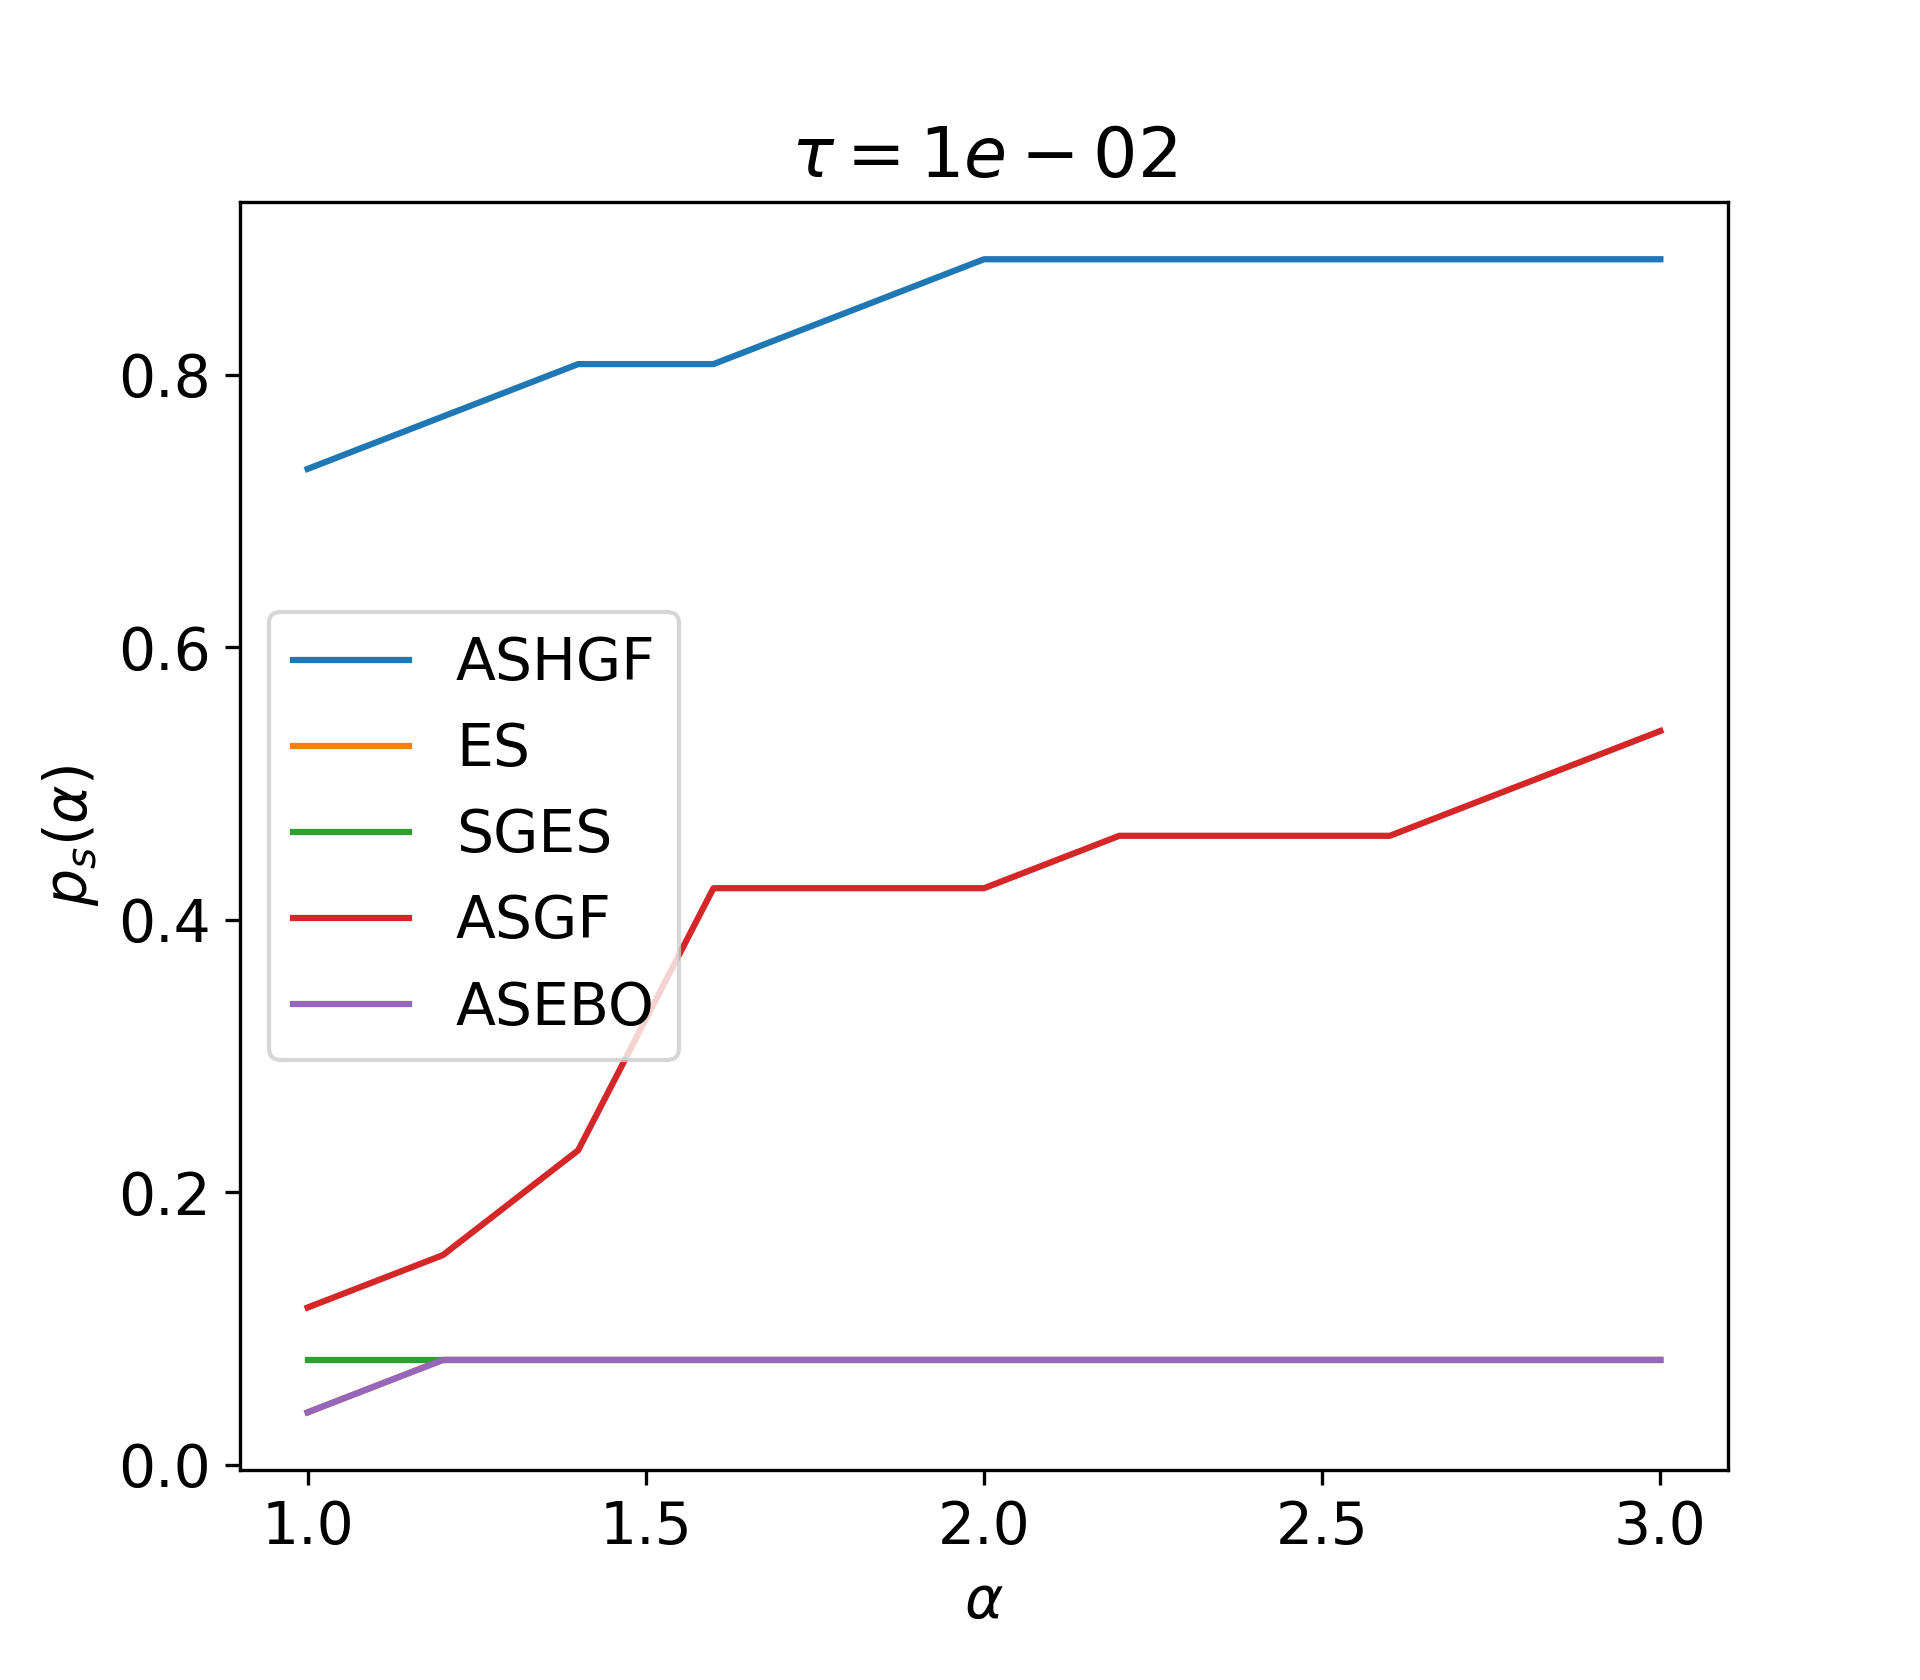
\includegraphics[width=1\textwidth]{figures/performance_profiles/10/performance_profile_10_100000000_1e-02.png}
	\end{subfigure}%
	\begin{subfigure}{0.3\textwidth}
		\centering 
		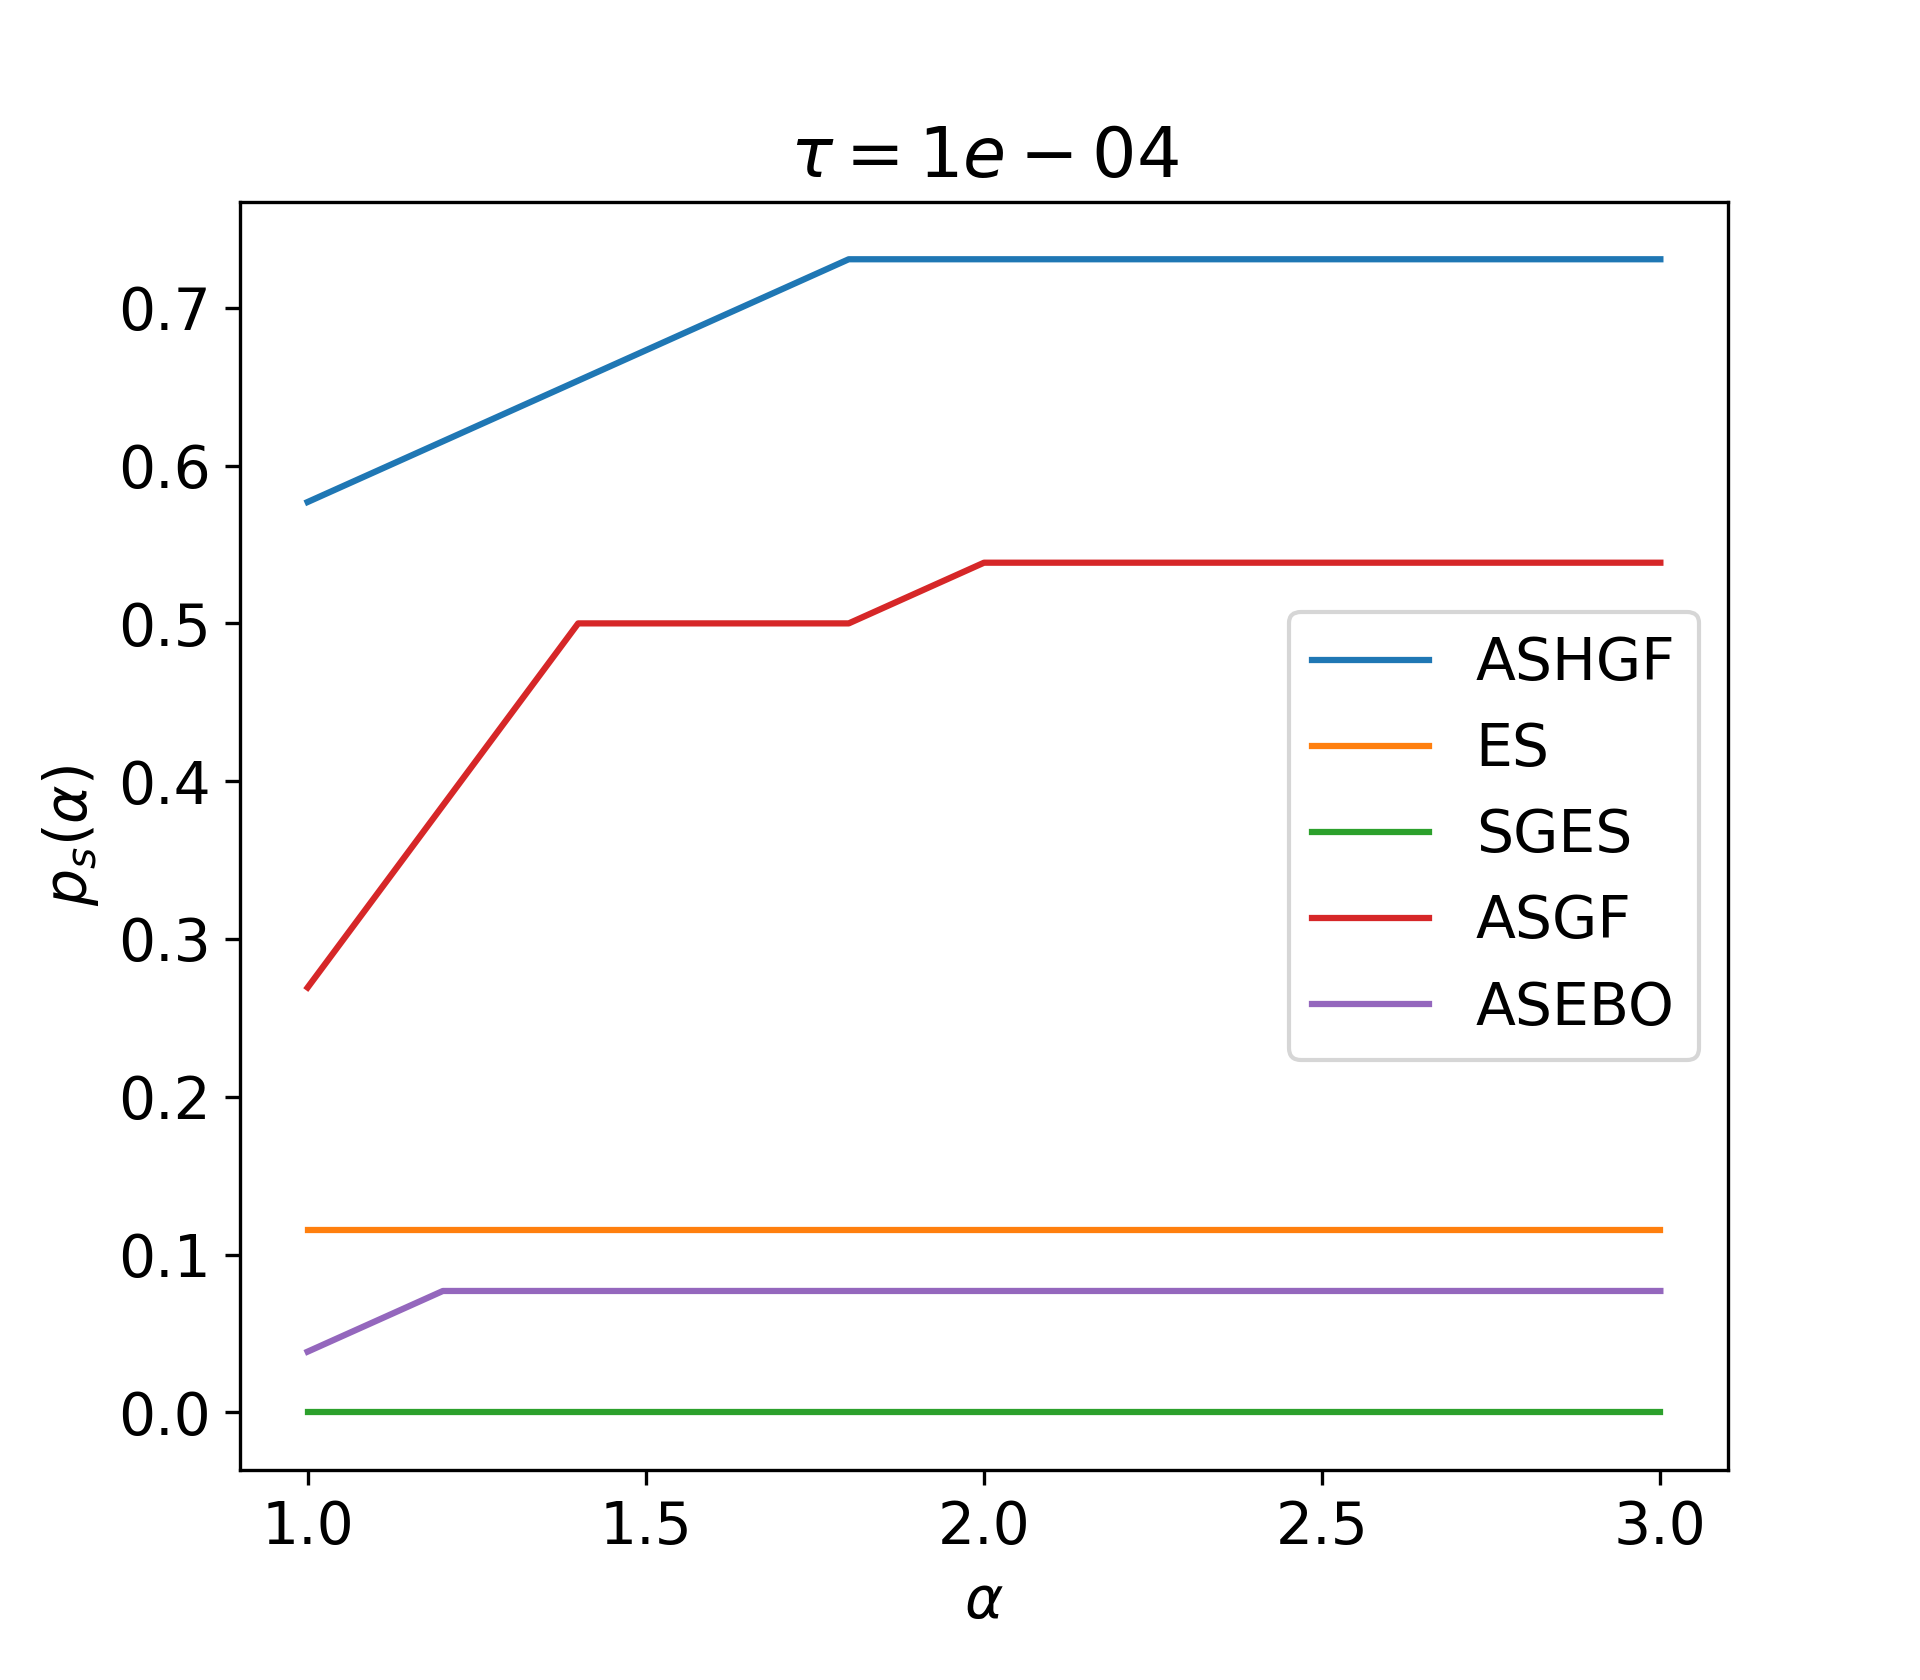
\includegraphics[width=1\textwidth]{figures/performance_profiles/10/performance_profile_10_100000000_1e-04.png}
	\end{subfigure}
	\begin{subfigure}{0.3\textwidth}
		\centering 
		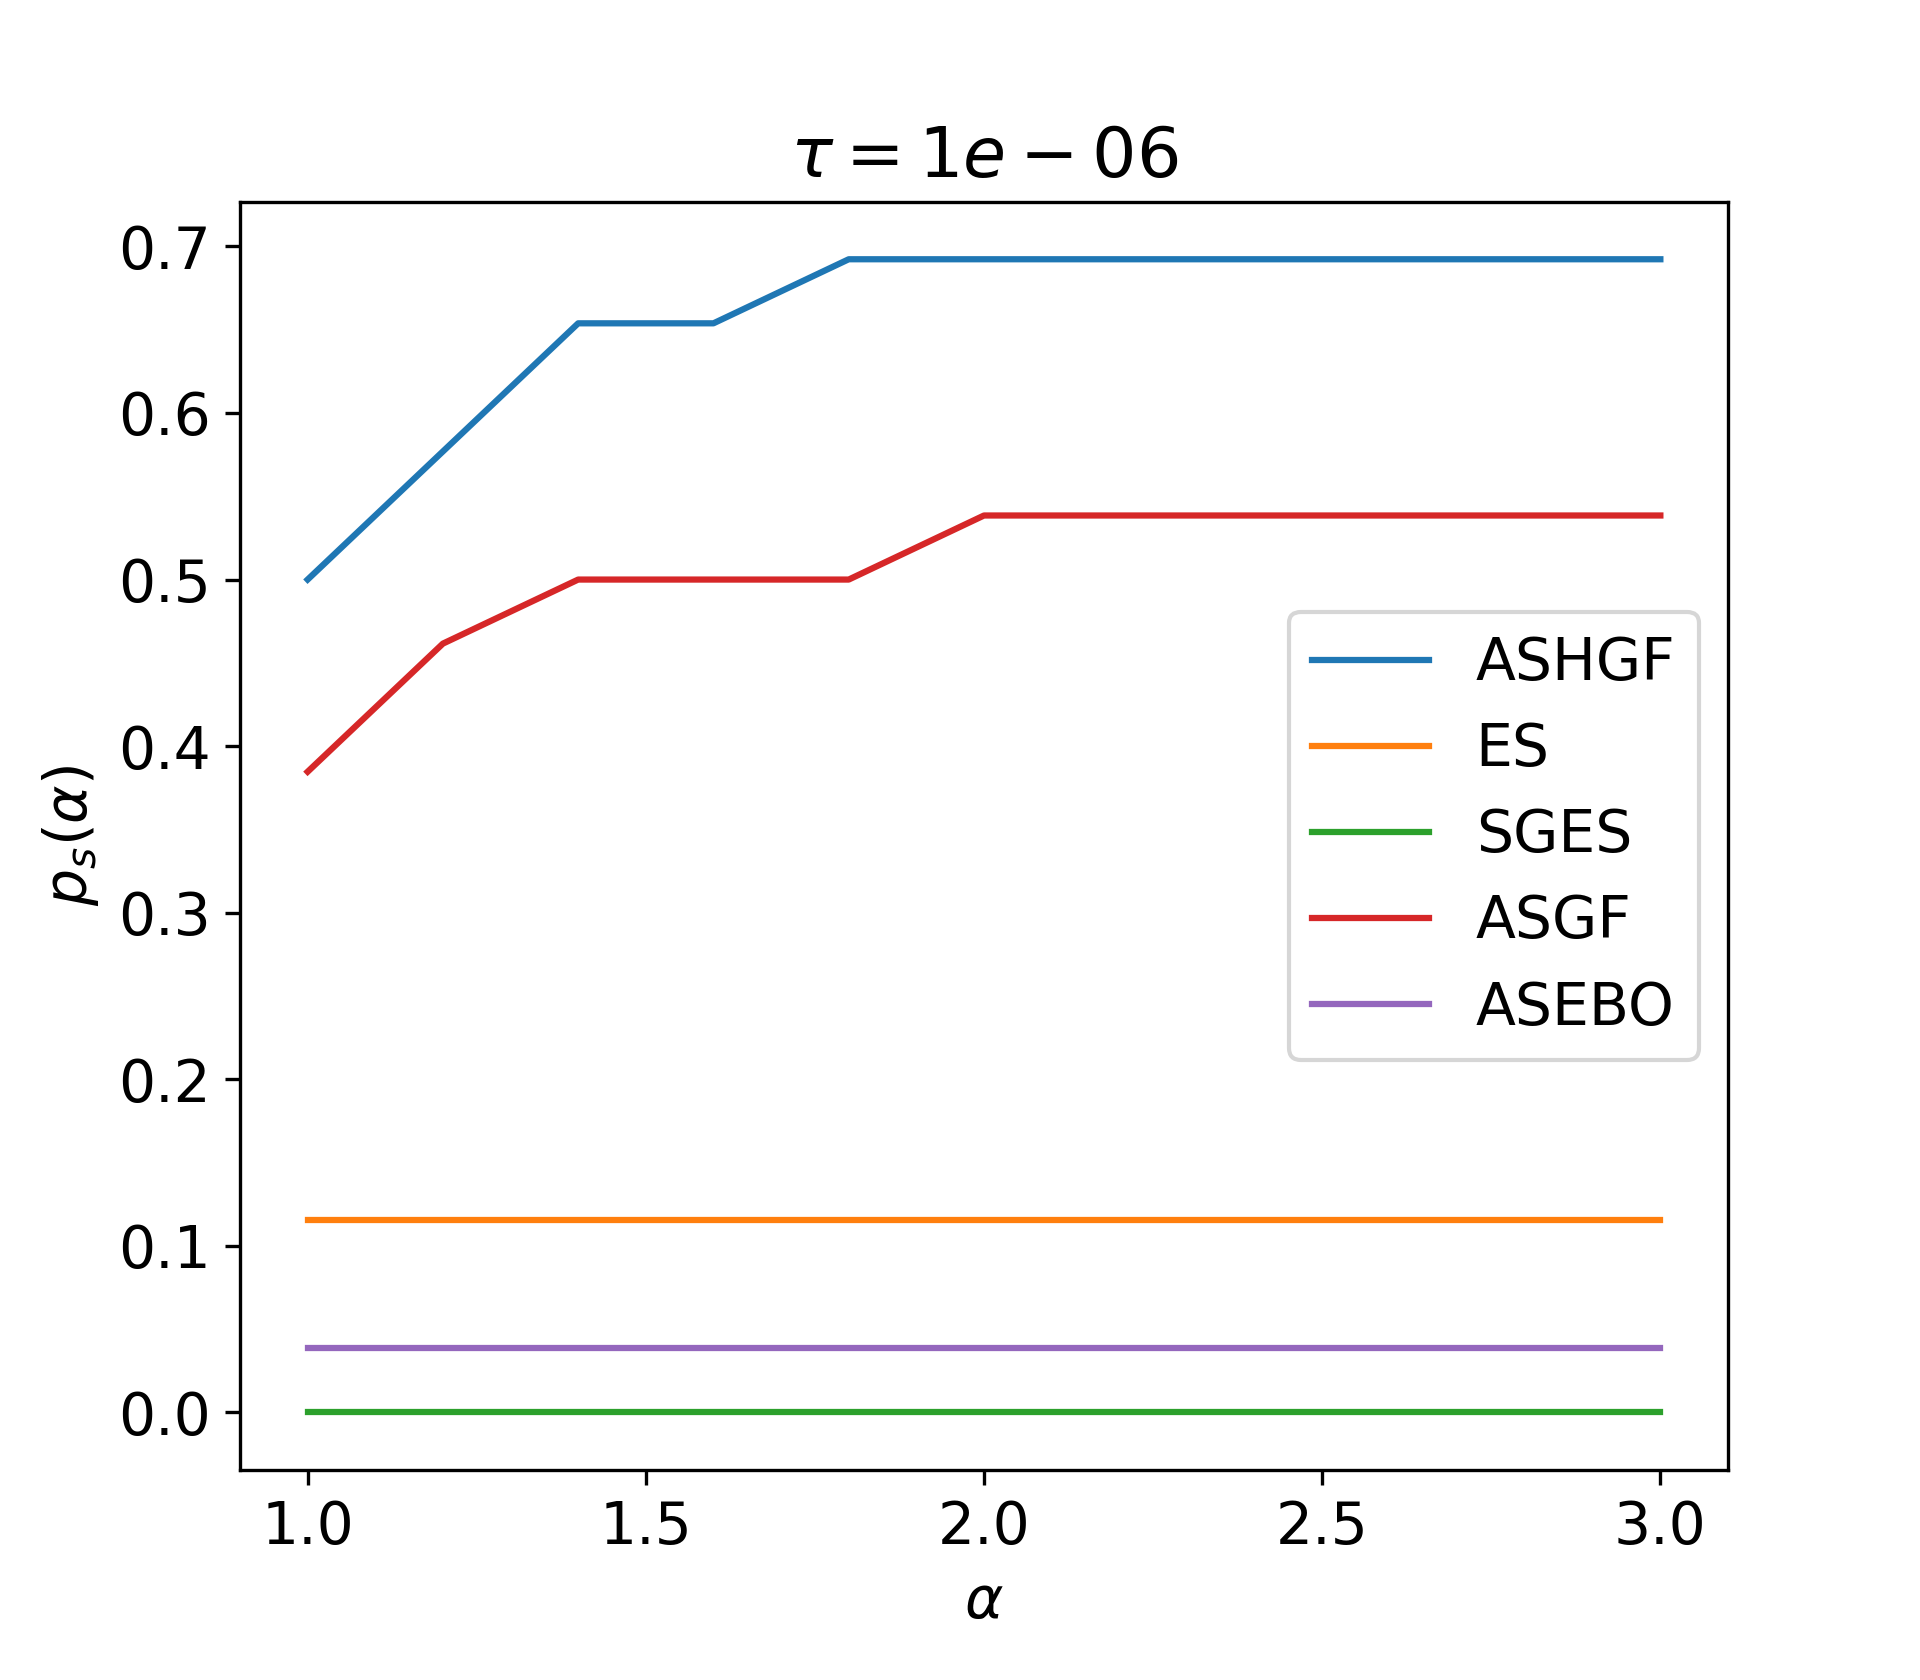
\includegraphics[width=1\textwidth]{figures/performance_profiles/10/performance_profile_10_100000000_1e-06.png}
	\end{subfigure}
	\centering
	\begin{subfigure}{0.3\textwidth}
		\centering 
		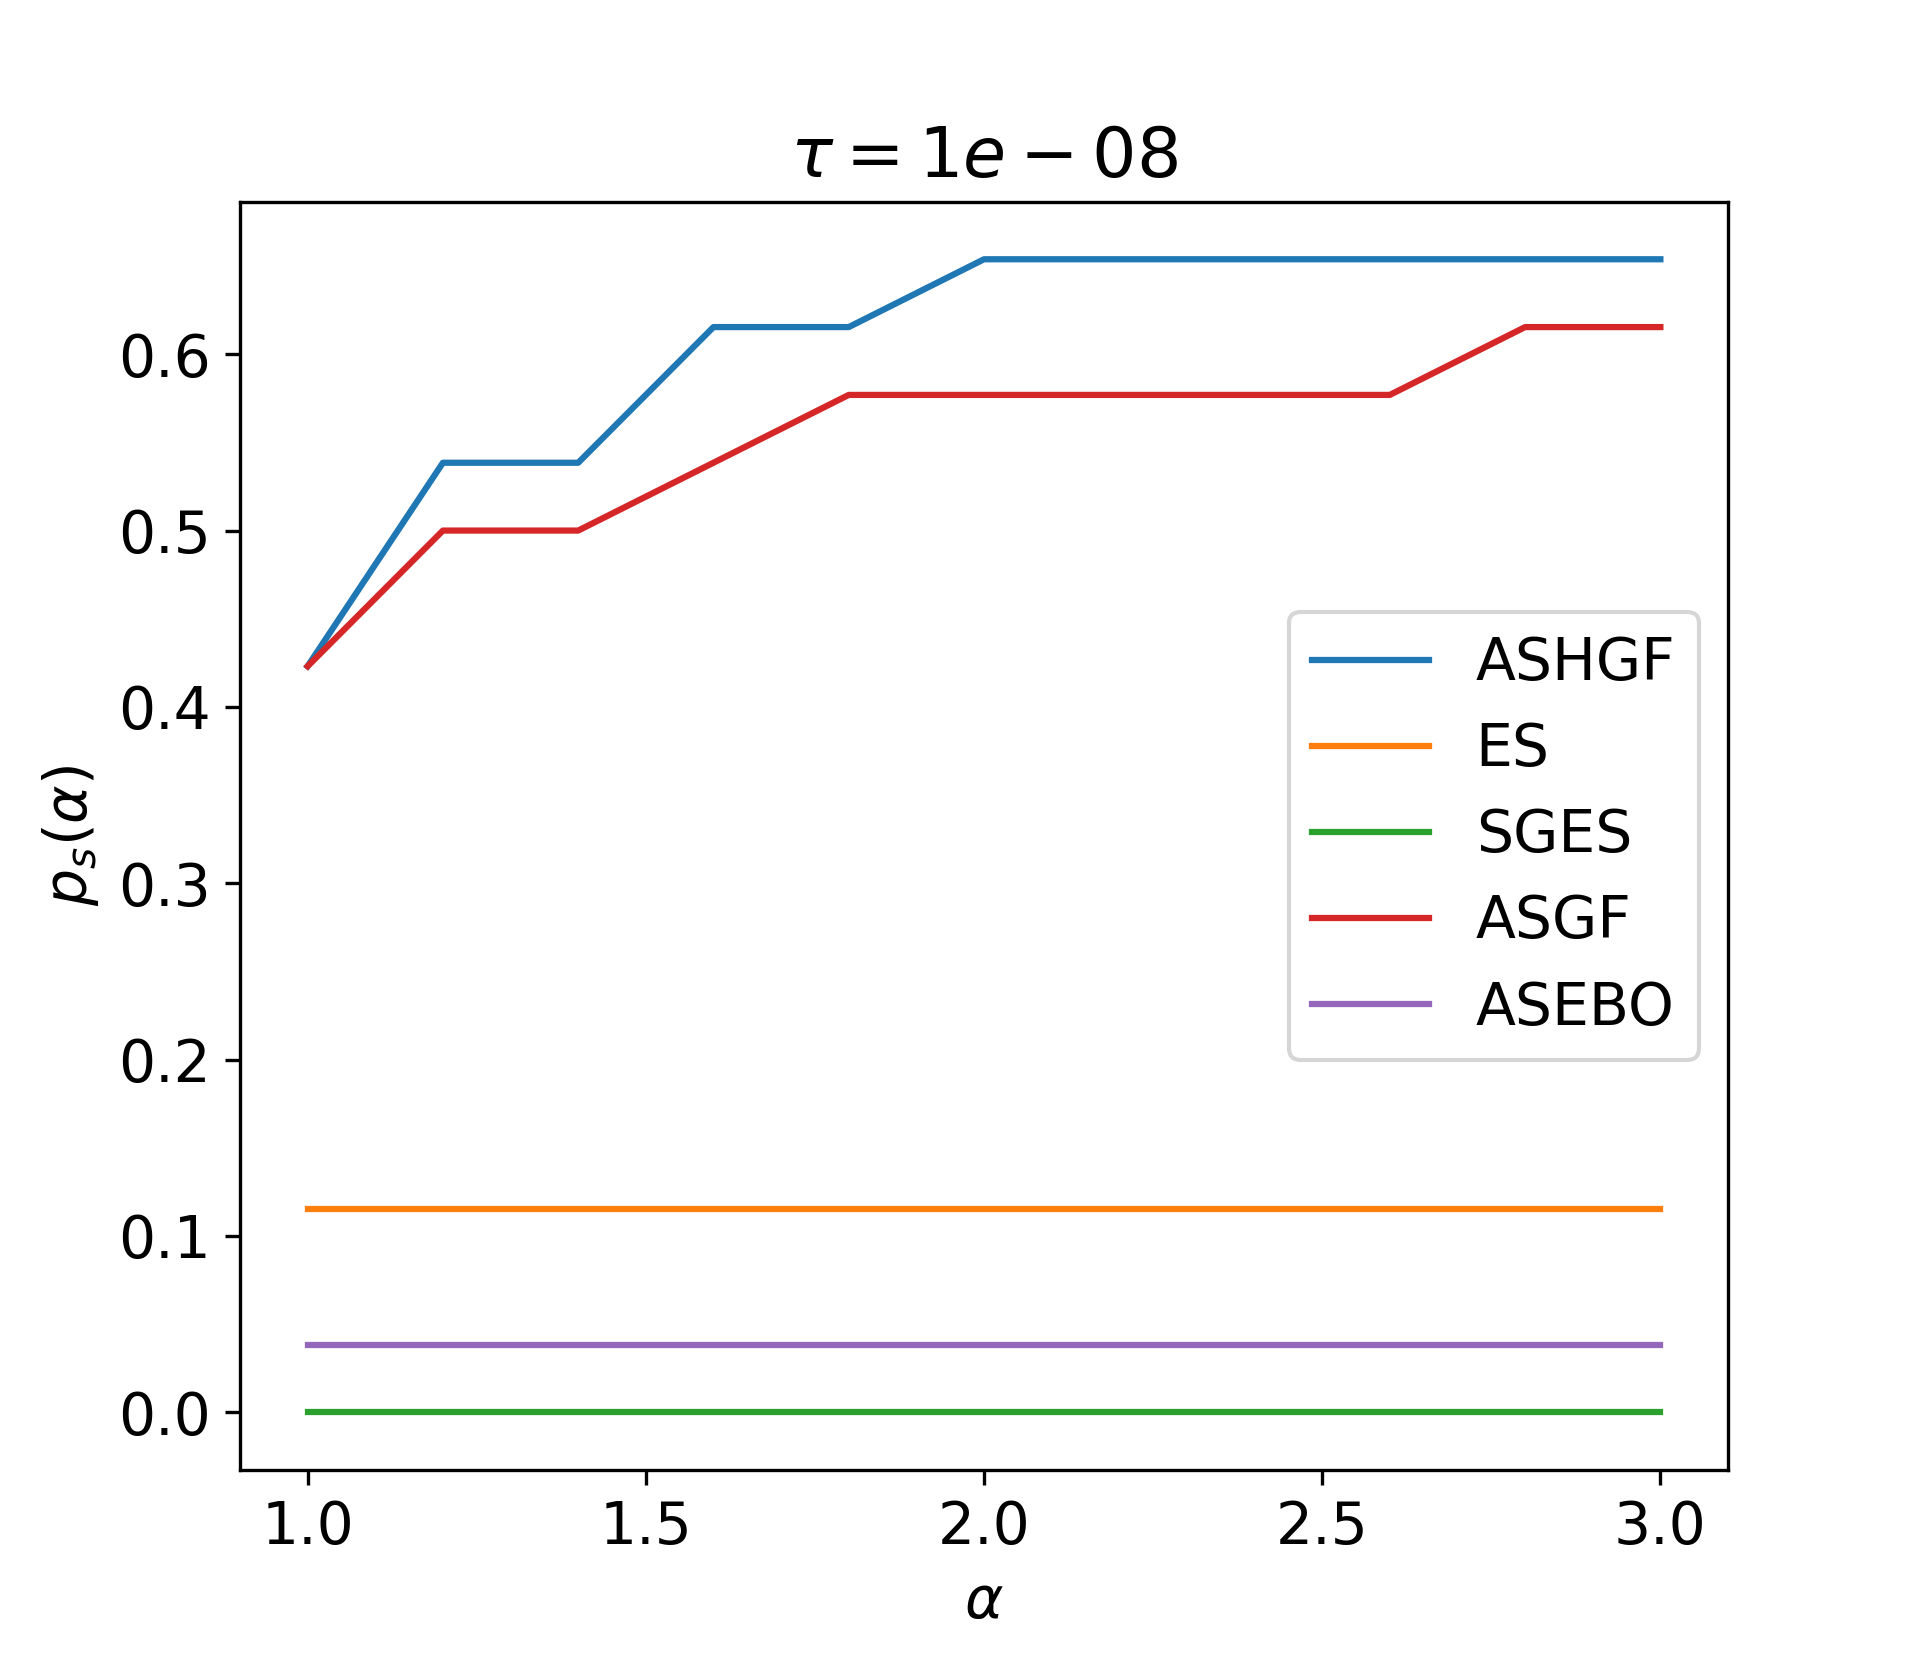
\includegraphics[width=1\textwidth]{figures/performance_profiles/10/performance_profile_10_100000000_1e-08.png}
	\end{subfigure}%
	\begin{subfigure}{0.3\textwidth}
		\centering 
		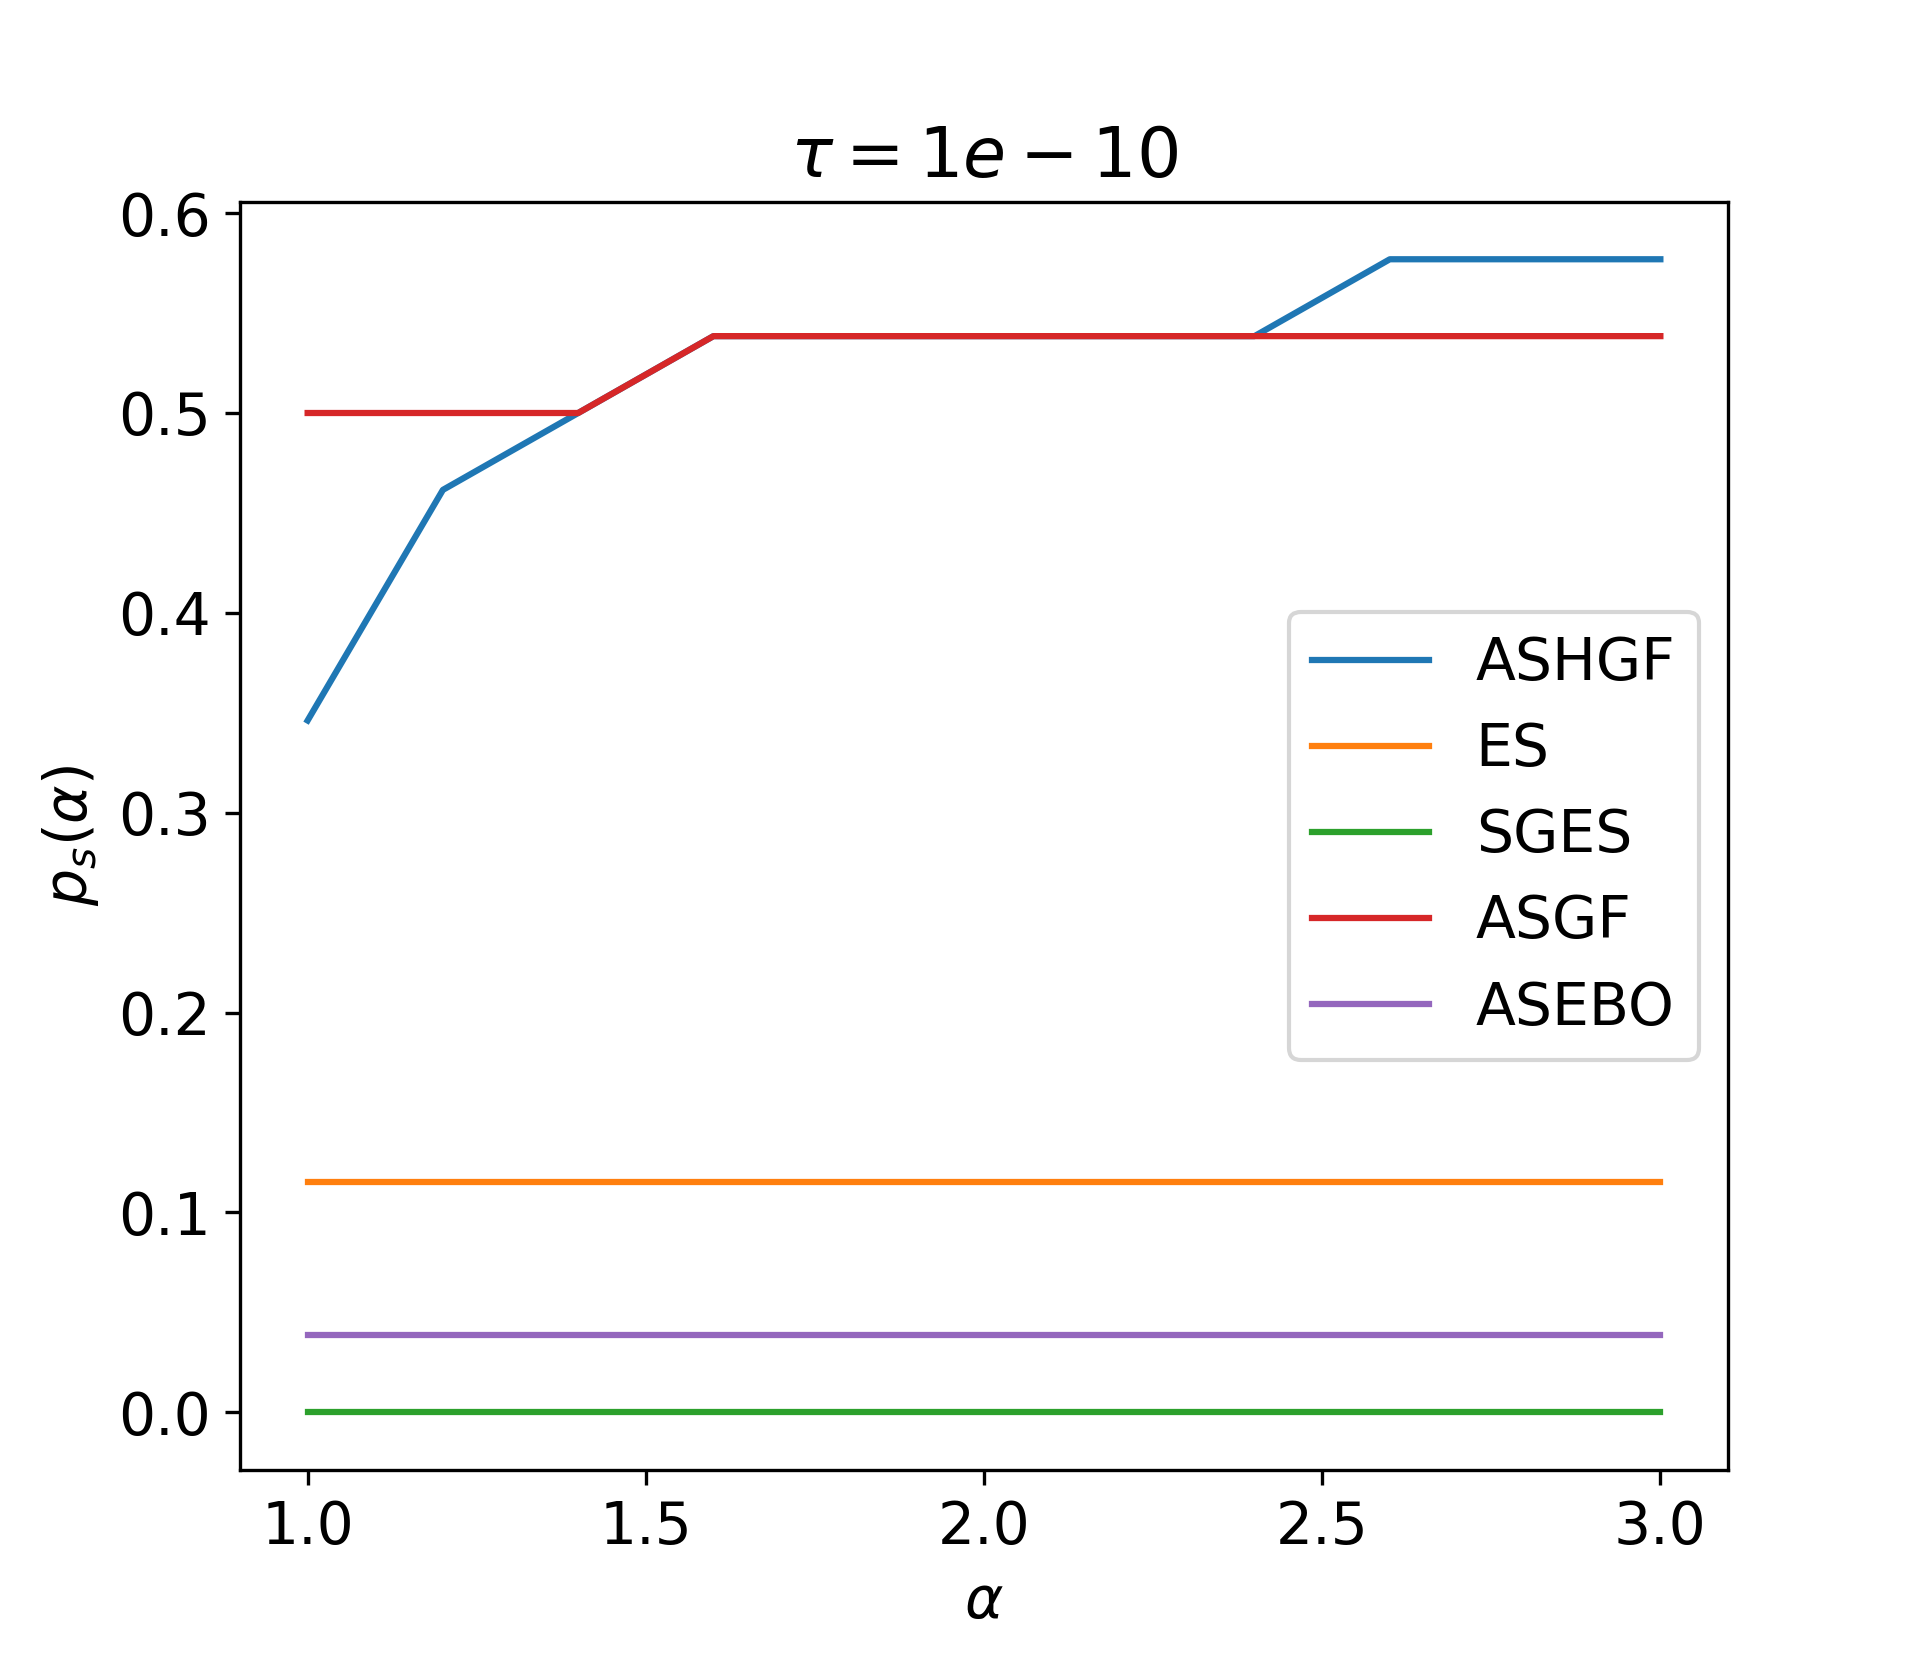
\includegraphics[width=1\textwidth]{figures/performance_profiles/10/performance_profile_10_100000000_1e-10.png}
	\end{subfigure}
	\caption{Performance profiles with $\mu_L = 10^{8}$}
	\label{PerformanceProfiles10Mu100000000}
\end{figure}

\subsubsection{Dimension 100}

\begin{figure}[H]
\centering
\begin{subfigure}{0.3\textwidth}
  \centering 
  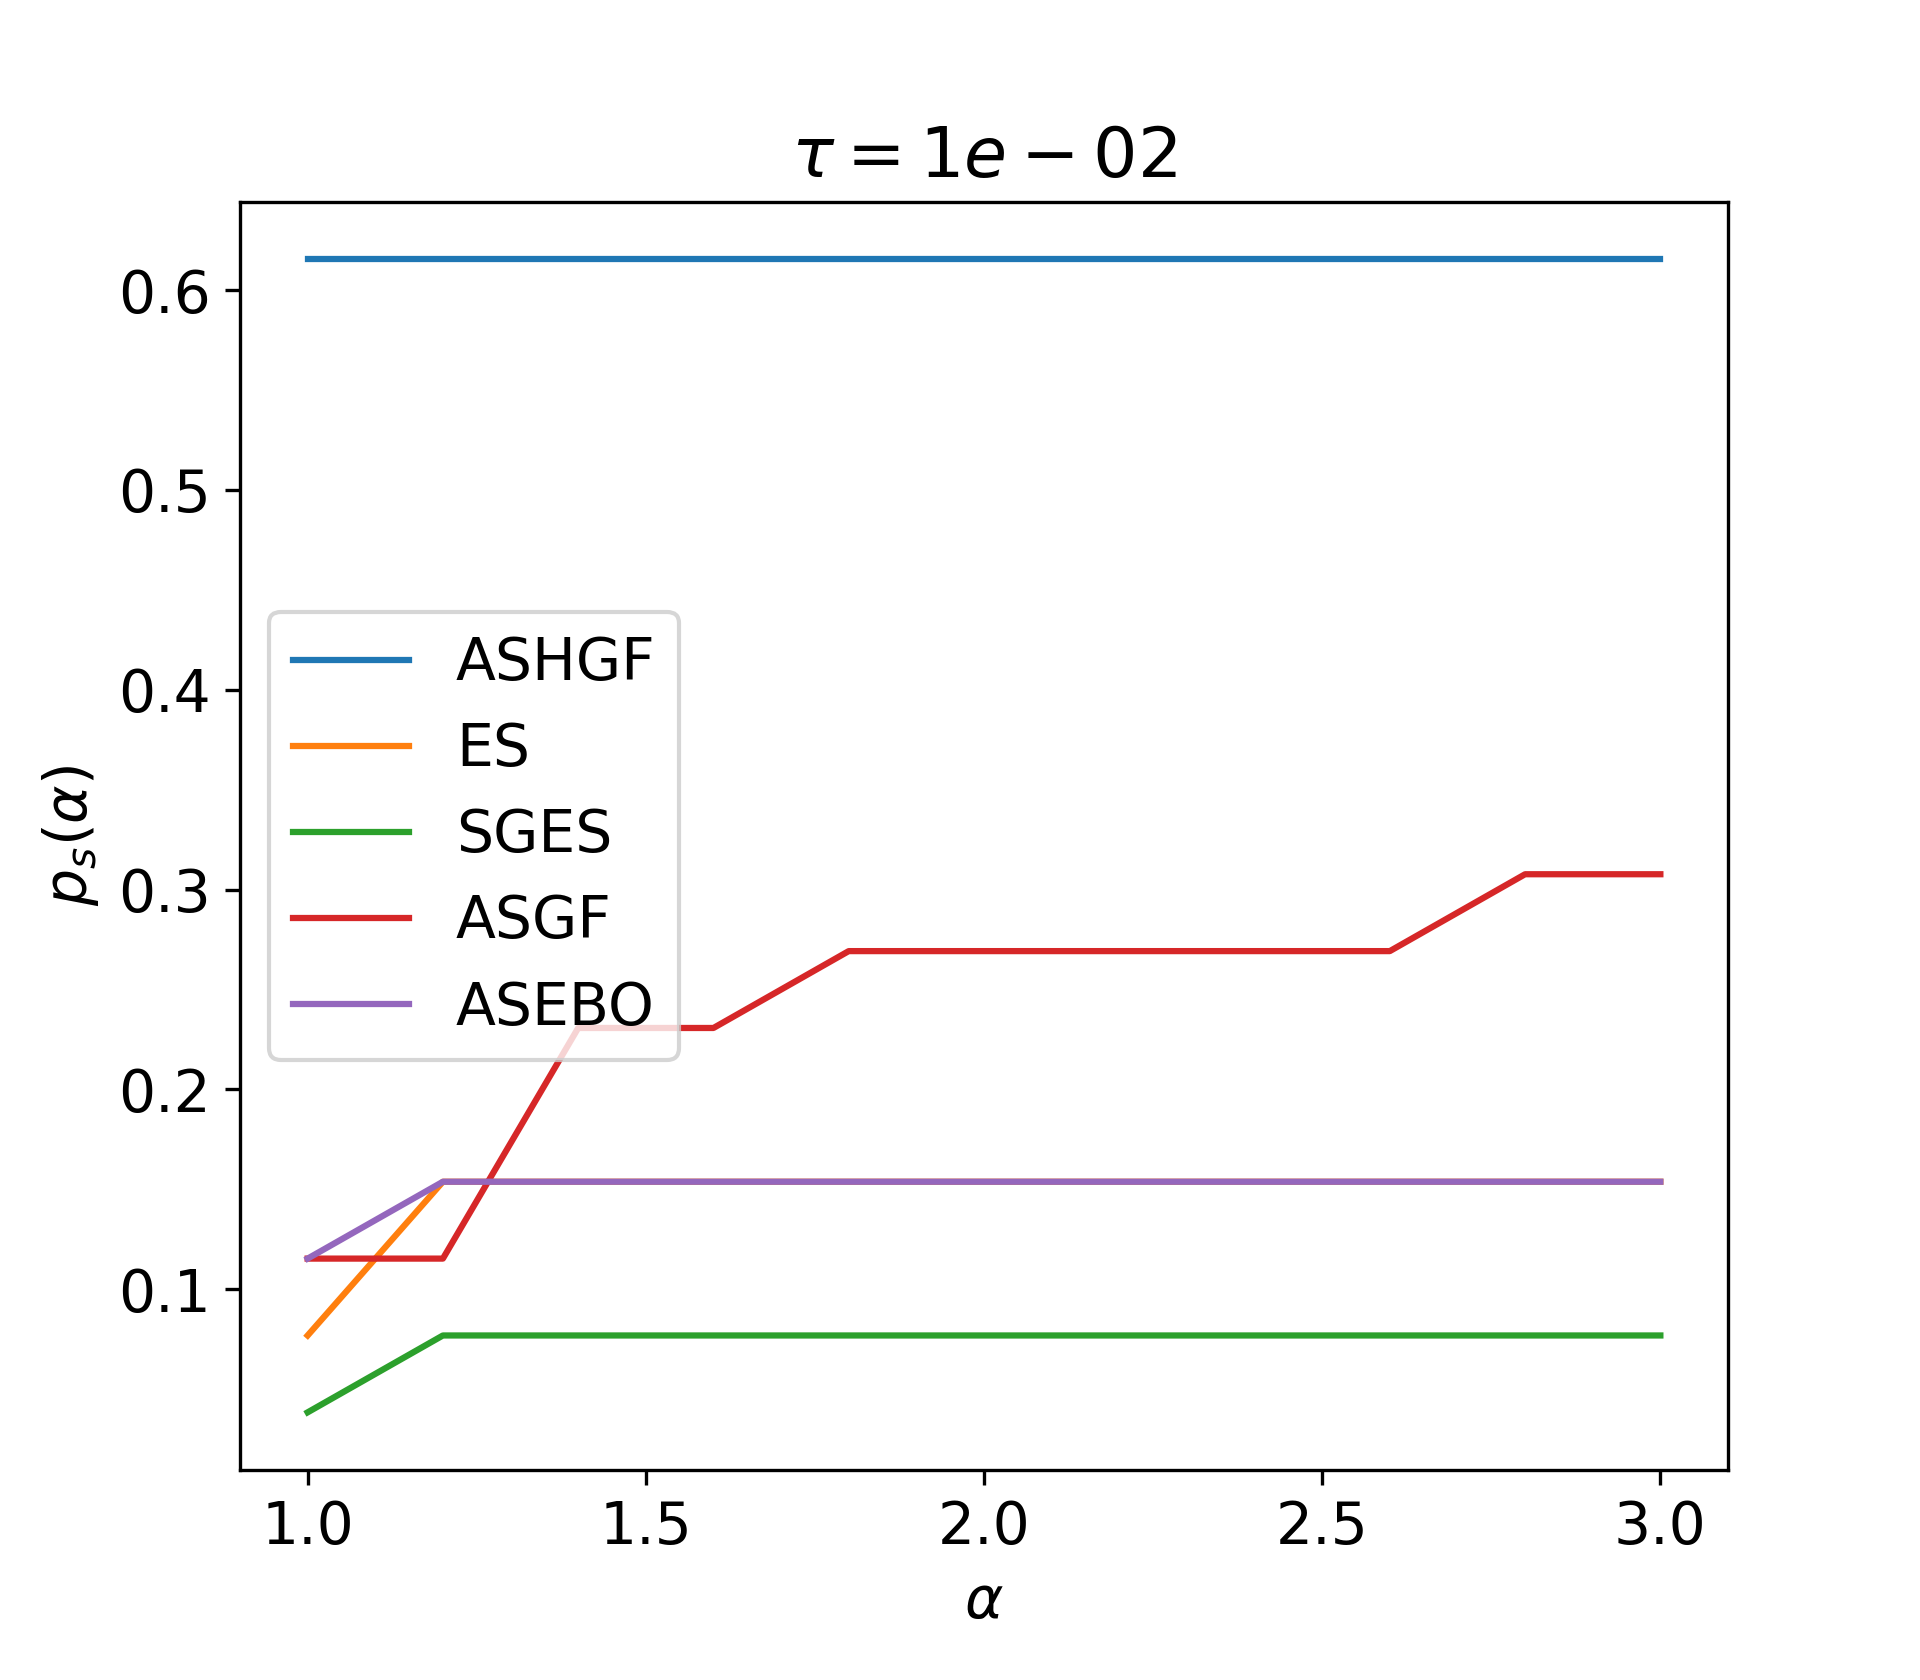
\includegraphics[width=1\textwidth]{figures/performance_profiles/100/performance_profile_100_10000_1e-02.png}
\end{subfigure}%
\begin{subfigure}{0.3\textwidth}
  \centering 
  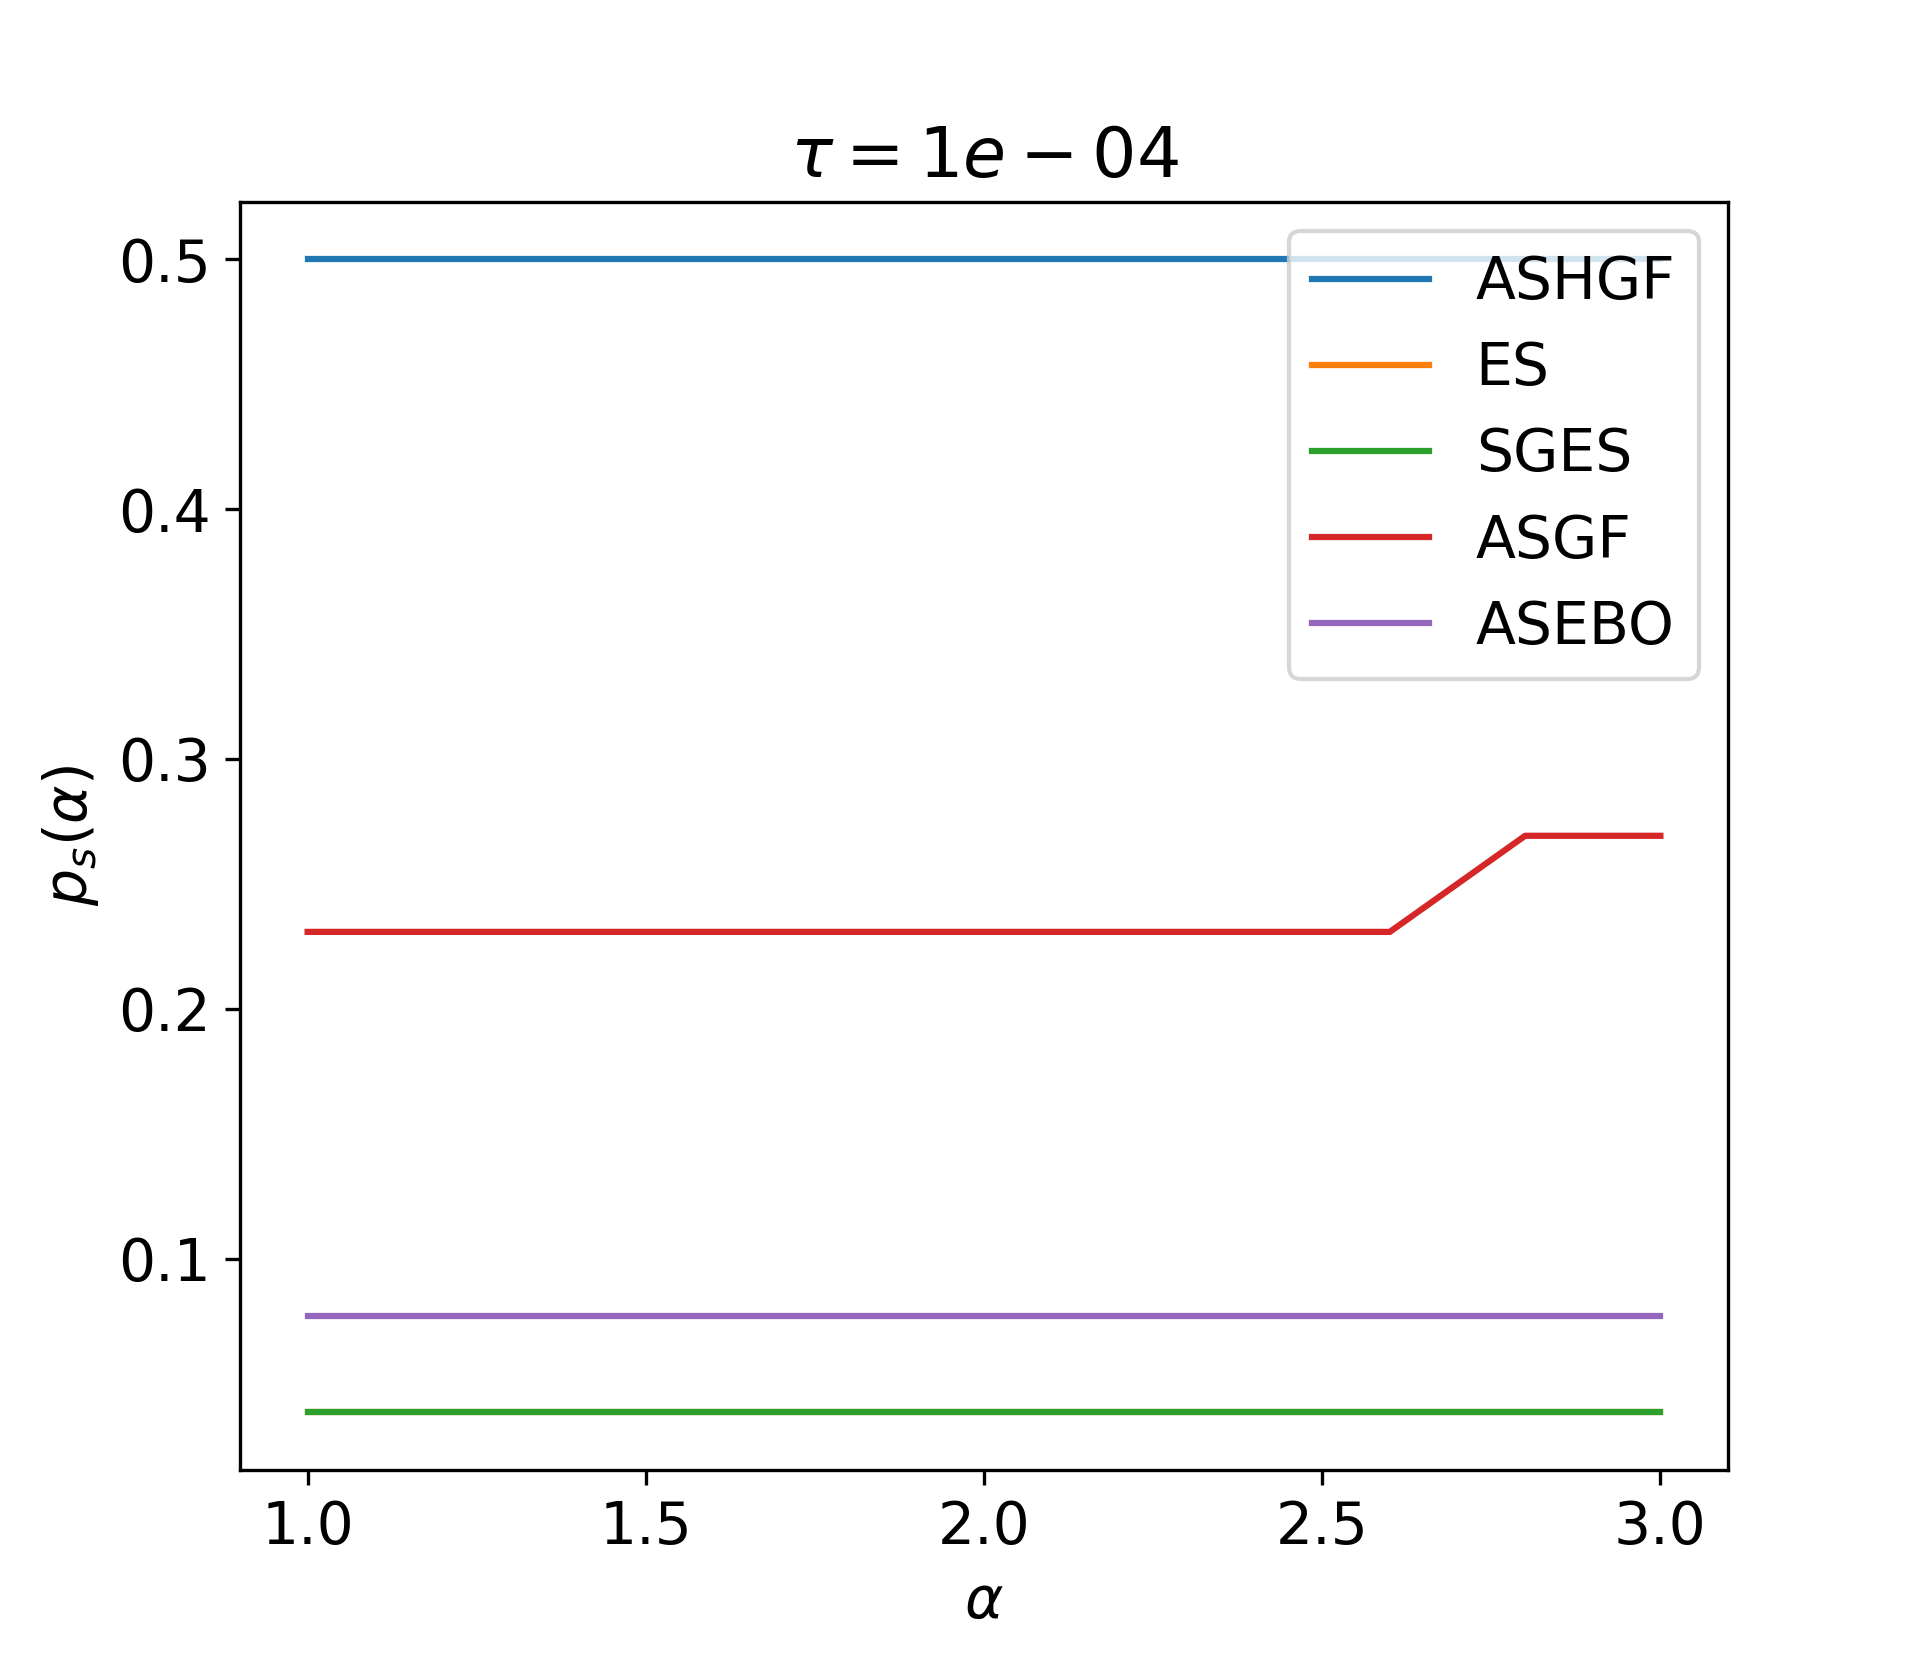
\includegraphics[width=1\textwidth]{figures/performance_profiles/100/performance_profile_100_10000_1e-04.png}
\end{subfigure}
\begin{subfigure}{0.3\textwidth}
  \centering 
  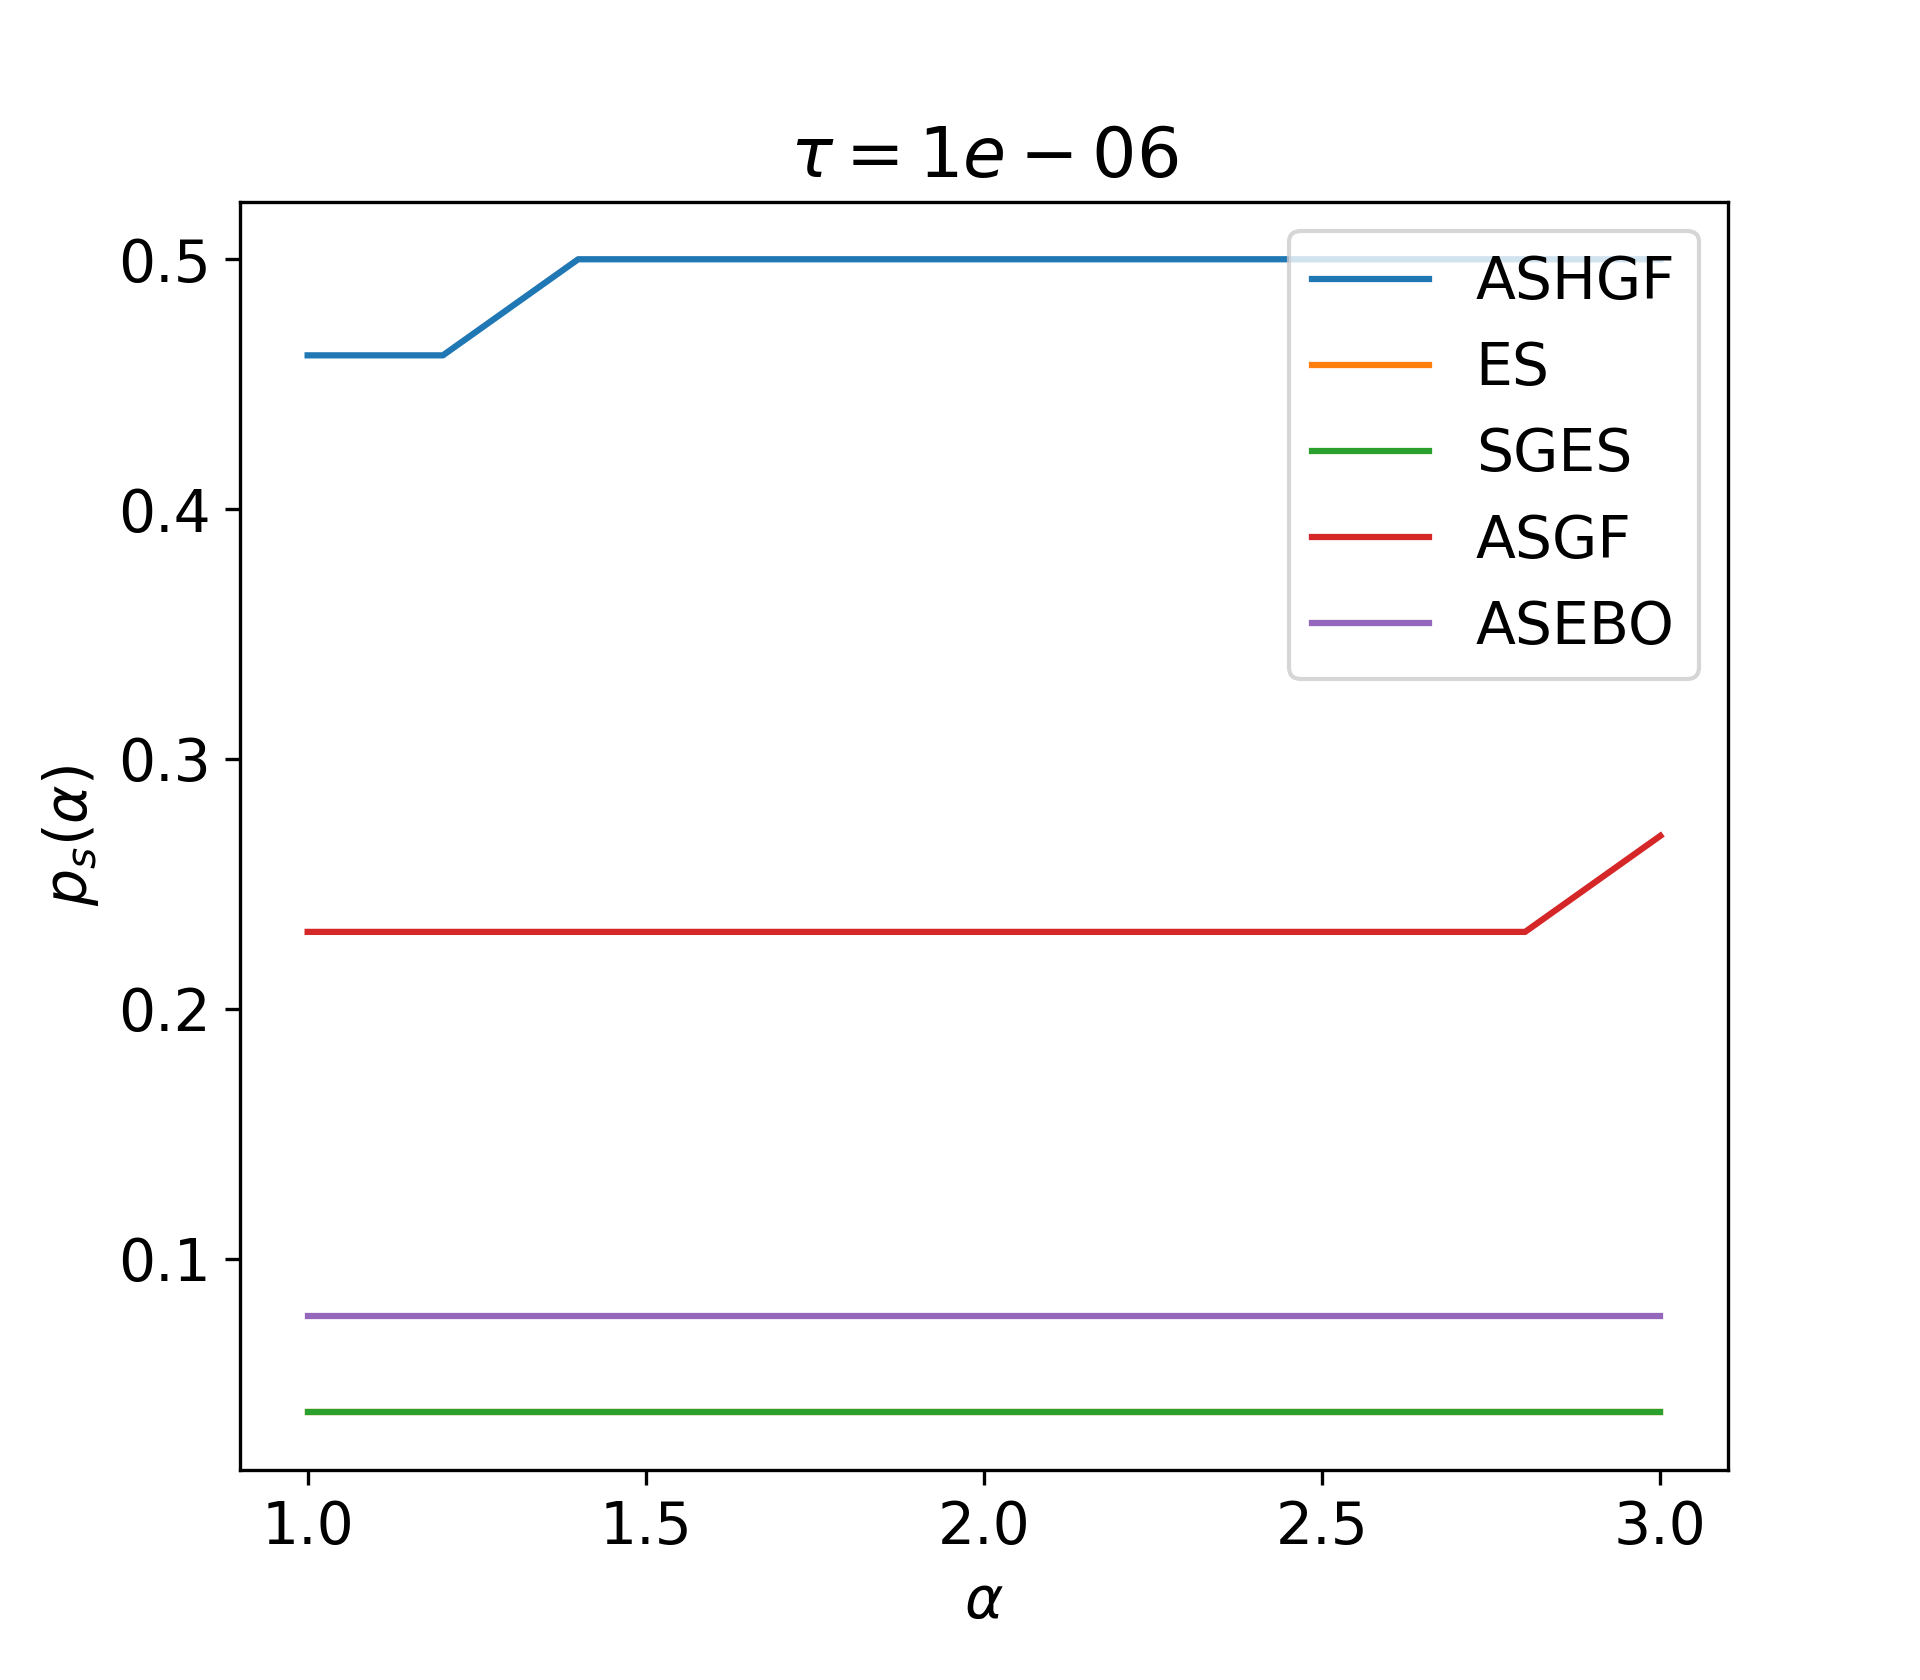
\includegraphics[width=1\textwidth]{figures/performance_profiles/100/performance_profile_100_10000_1e-06.png}
\end{subfigure}
\centering
\begin{subfigure}{0.3\textwidth}
  \centering 
  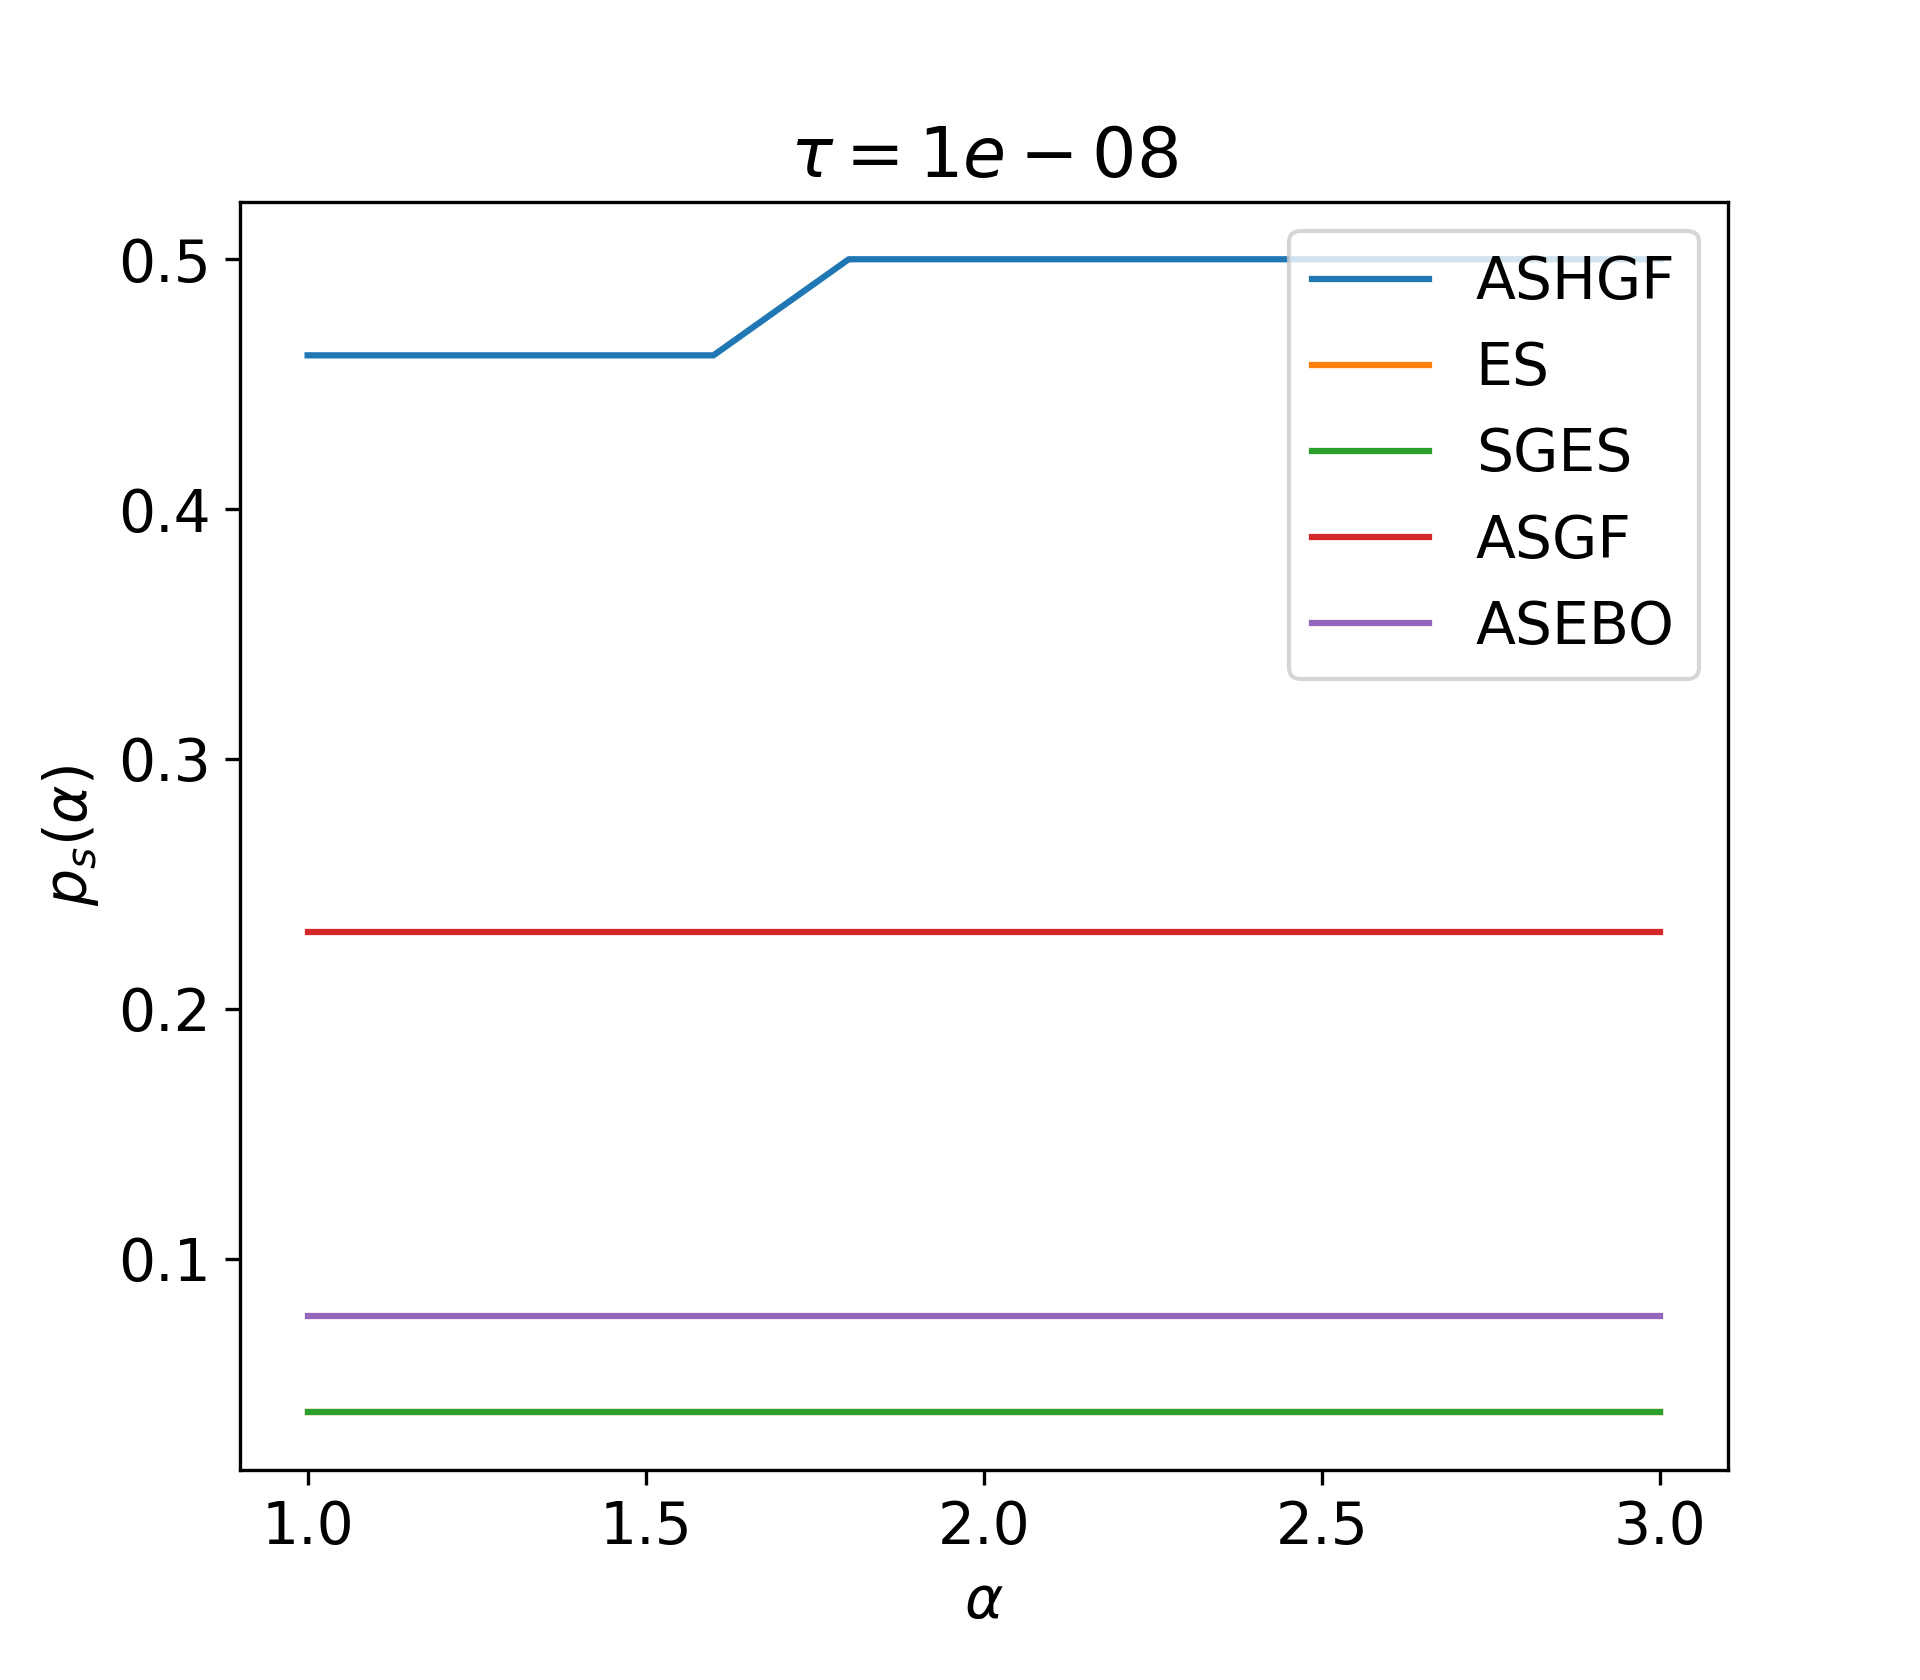
\includegraphics[width=1\textwidth]{figures/performance_profiles/100/performance_profile_100_10000_1e-08.png}
\end{subfigure}%
\begin{subfigure}{0.3\textwidth}
  \centering 
  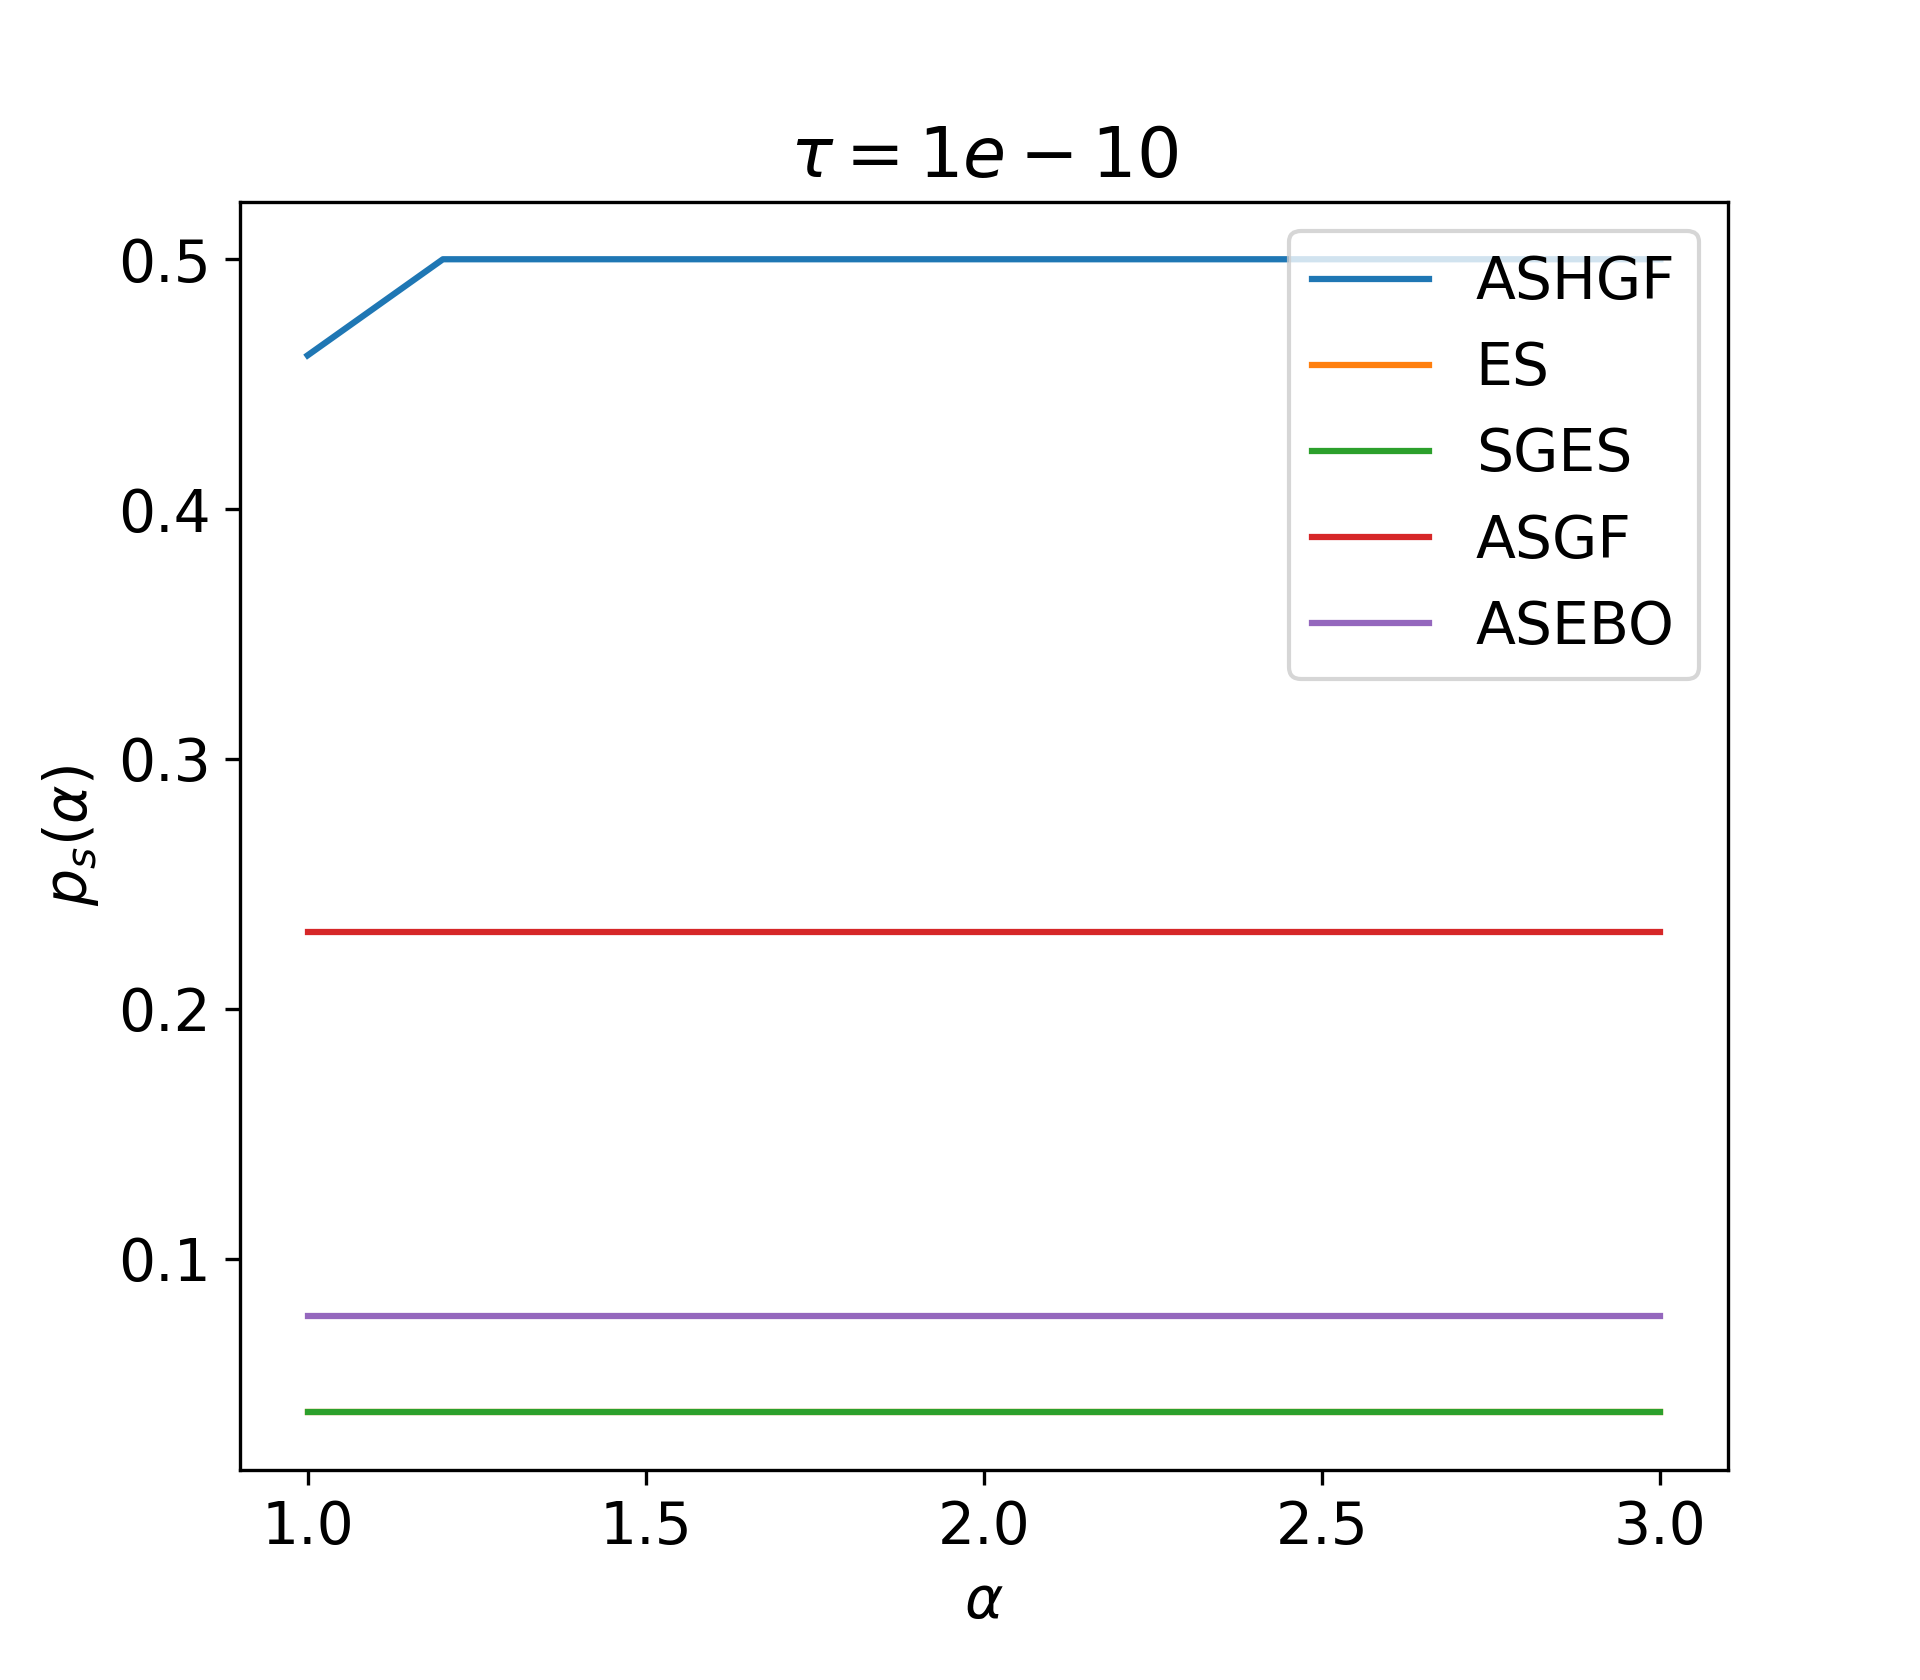
\includegraphics[width=1\textwidth]{figures/performance_profiles/100/performance_profile_100_10000_1e-10.png}
\end{subfigure}
\caption{Performance profiles with $\mu_L = 10^{4}$}
\label{PerformanceProfiles100Mu10000}
\end{figure}

\begin{figure}[H]
\centering
\begin{subfigure}{0.3\textwidth}
  \centering 
  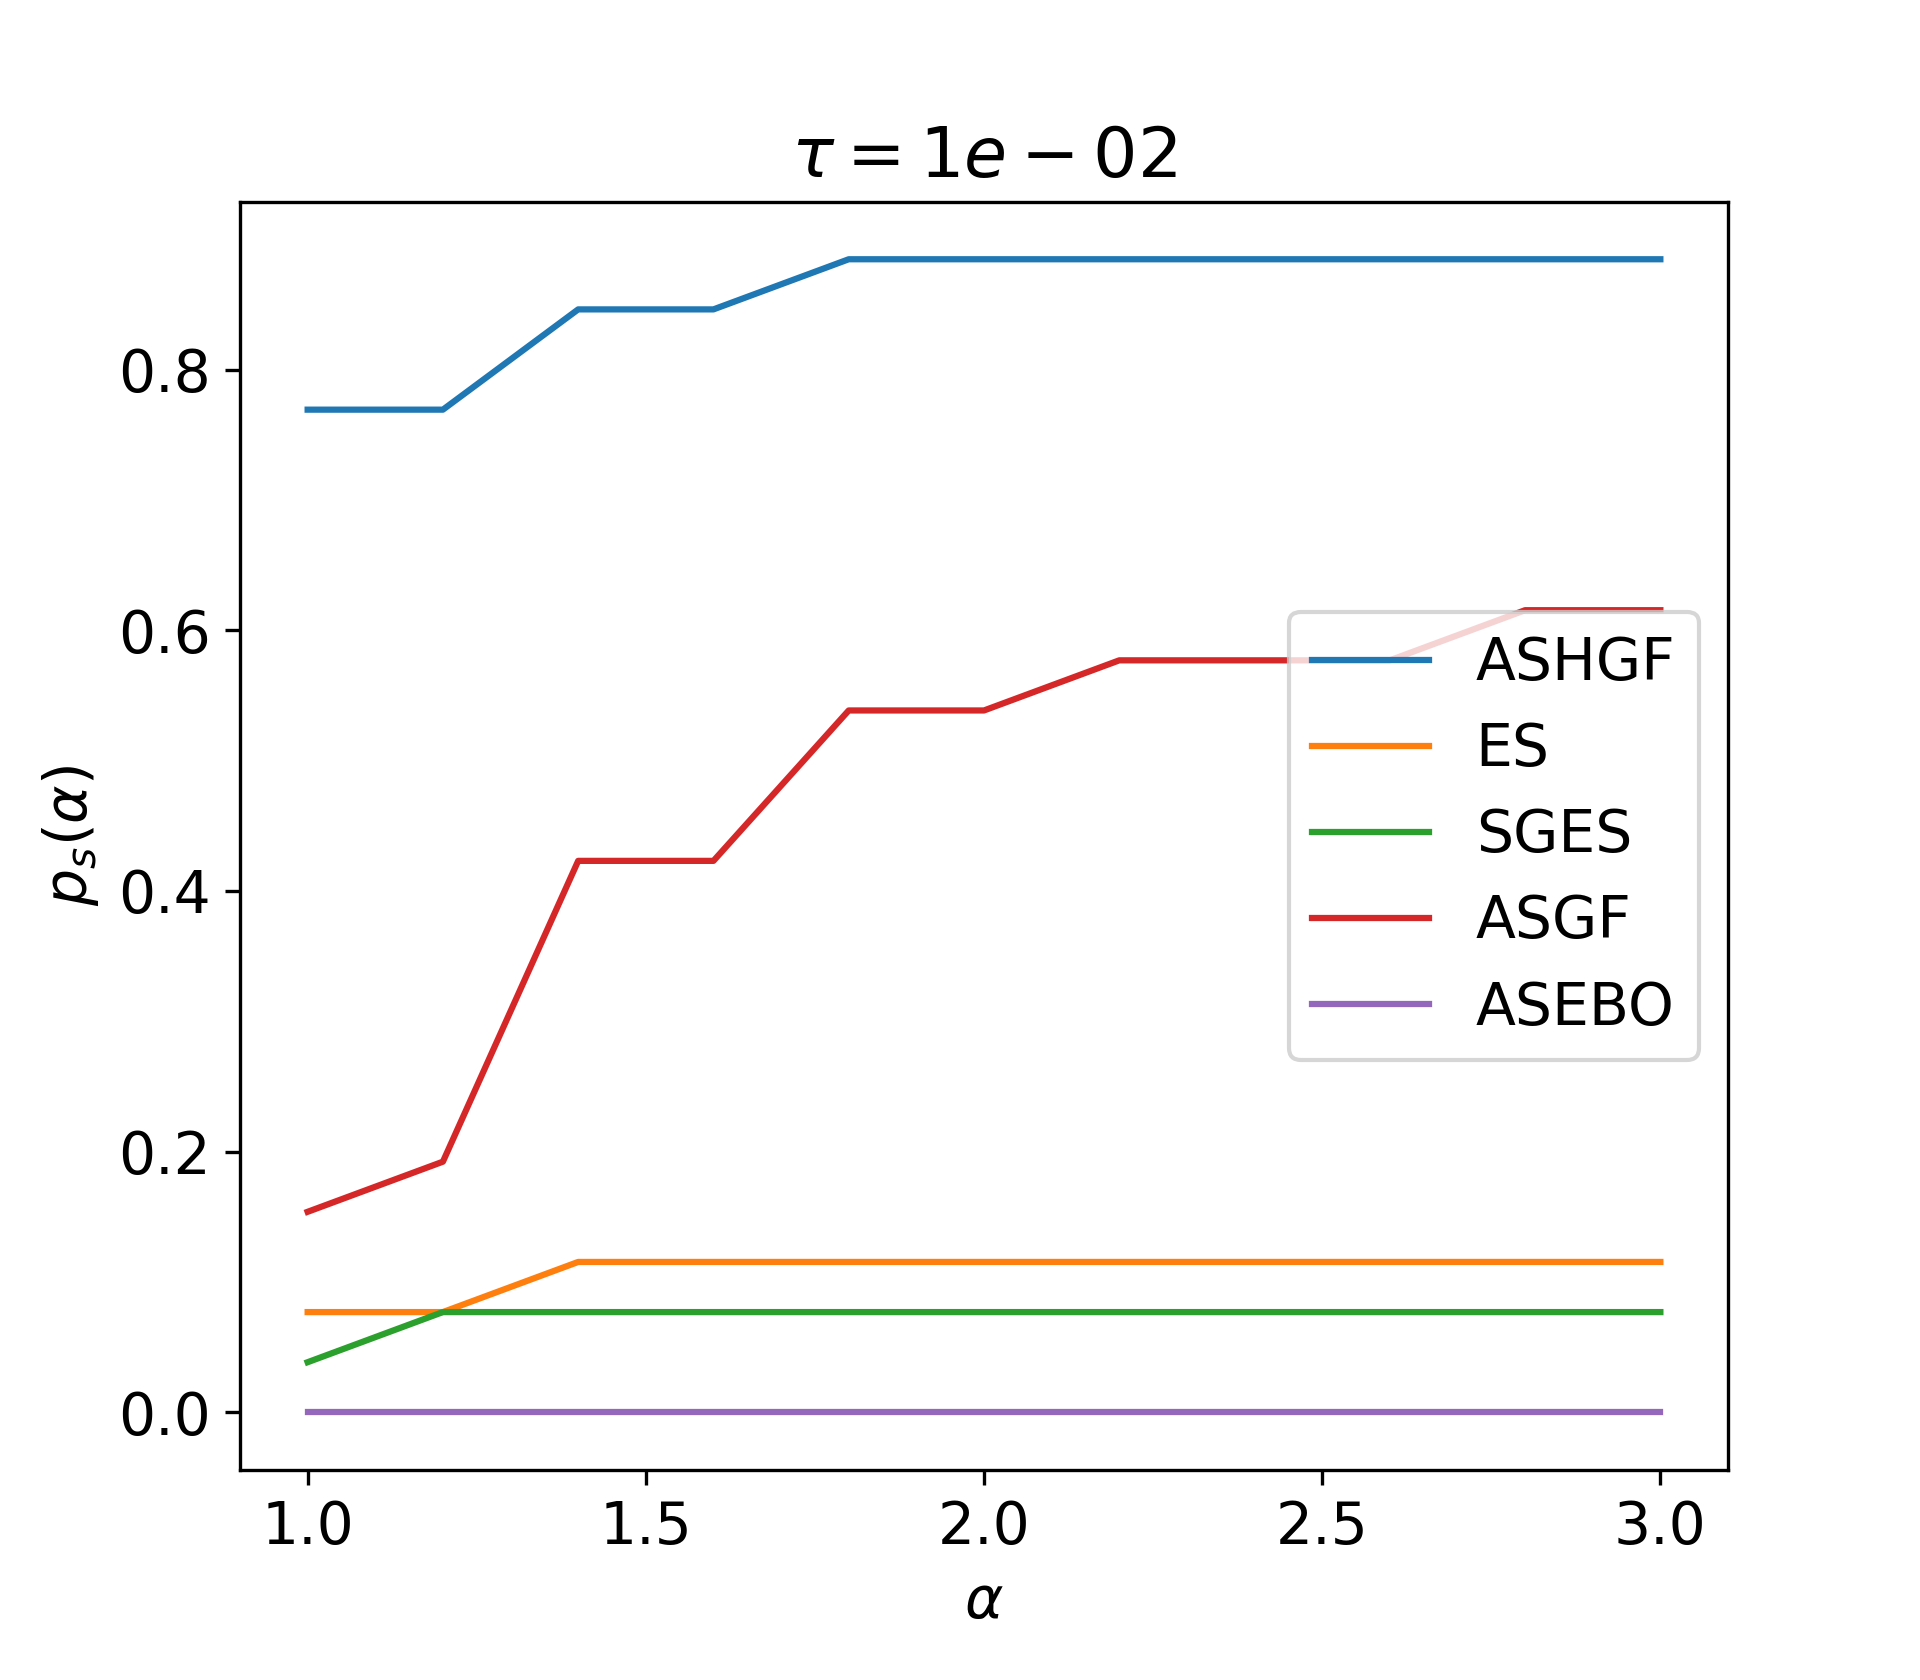
\includegraphics[width=1\textwidth]{figures/performance_profiles/100/performance_profile_100_100000_1e-02.png}
\end{subfigure}%
\begin{subfigure}{0.3\textwidth}
  \centering 
  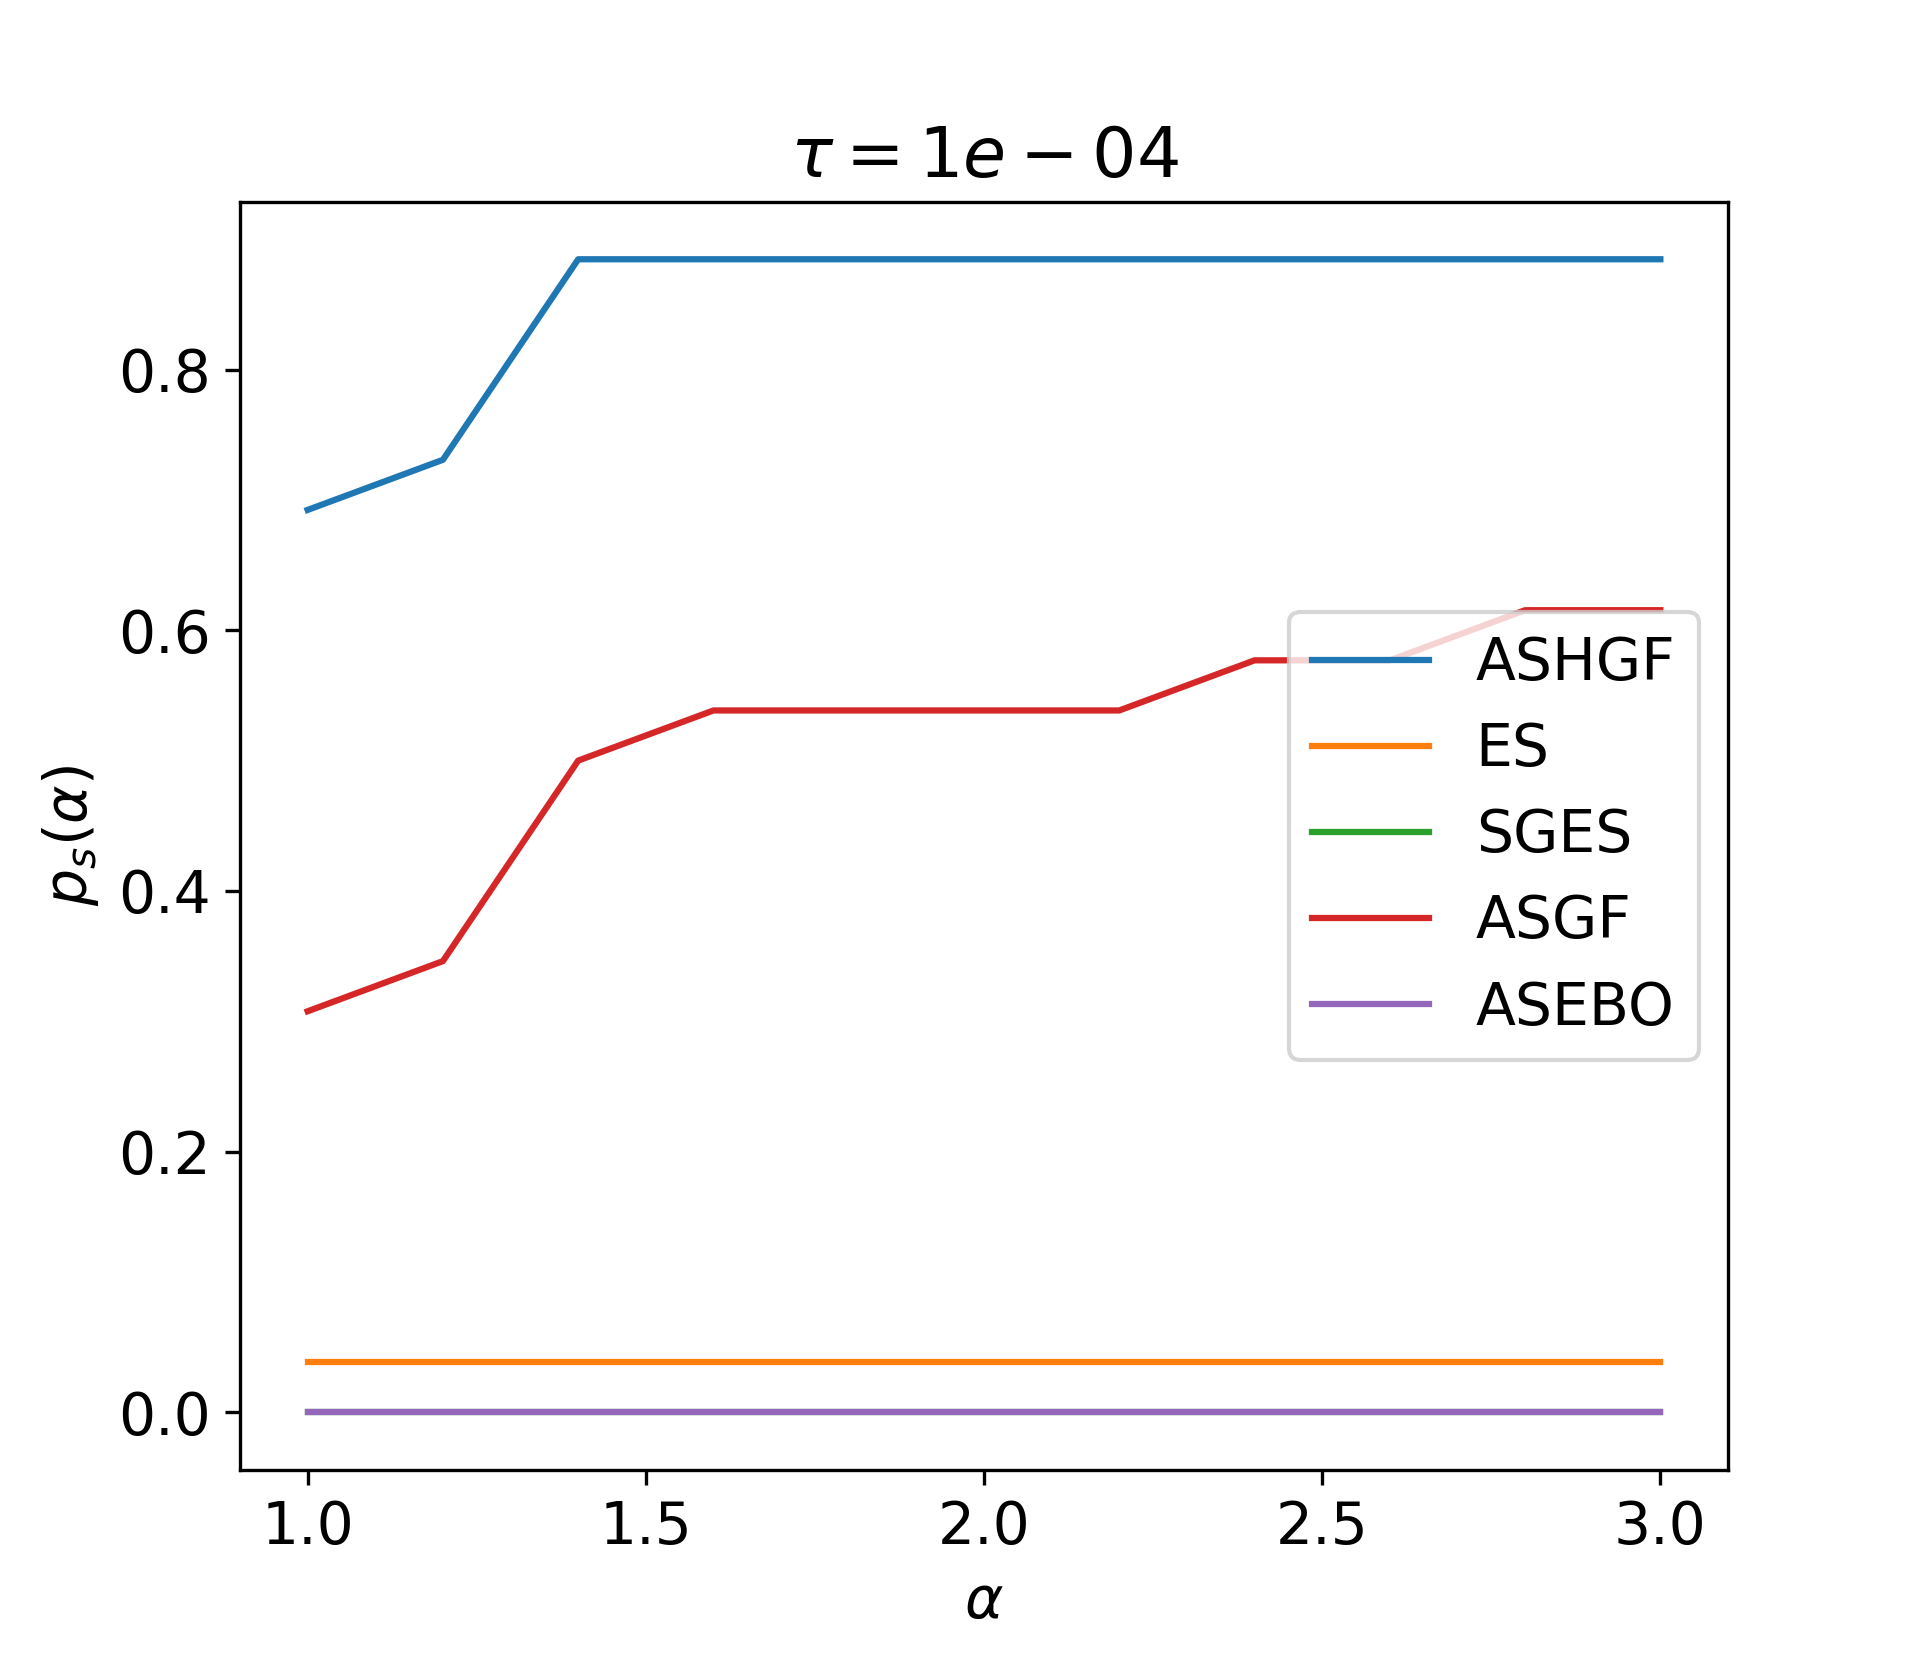
\includegraphics[width=1\textwidth]{figures/performance_profiles/100/performance_profile_100_100000_1e-04.png}
\end{subfigure}
\begin{subfigure}{0.3\textwidth}
  \centering 
  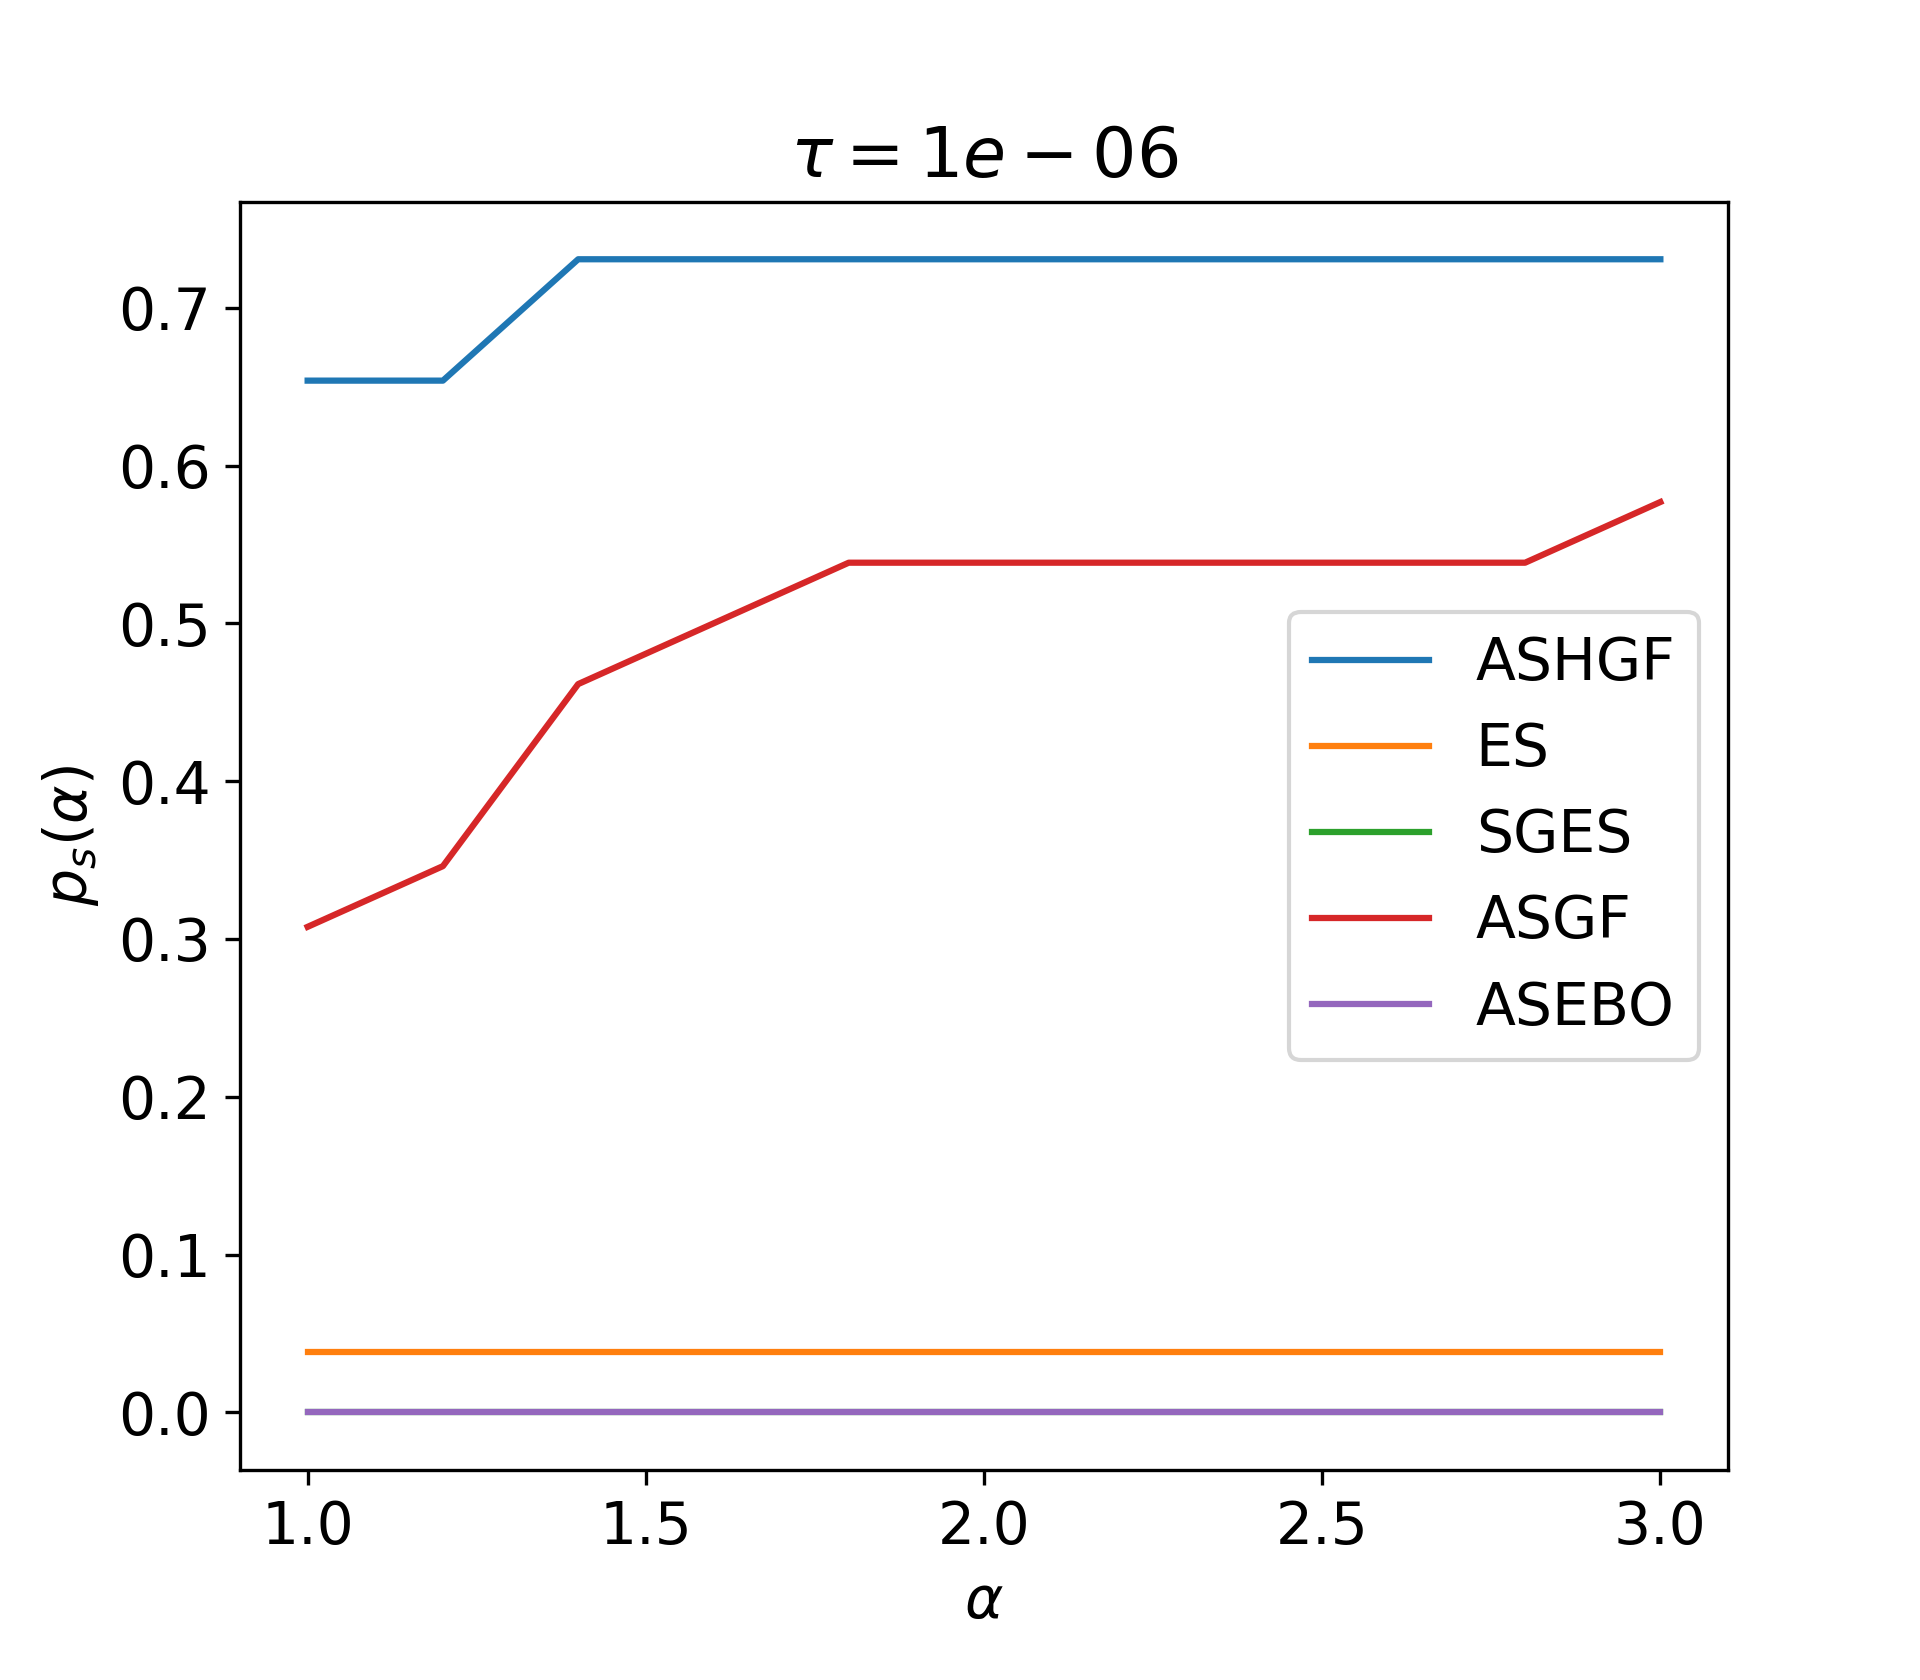
\includegraphics[width=1\textwidth]{figures/performance_profiles/100/performance_profile_100_100000_1e-06.png}
\end{subfigure}
\centering
\begin{subfigure}{0.3\textwidth}
  \centering 
  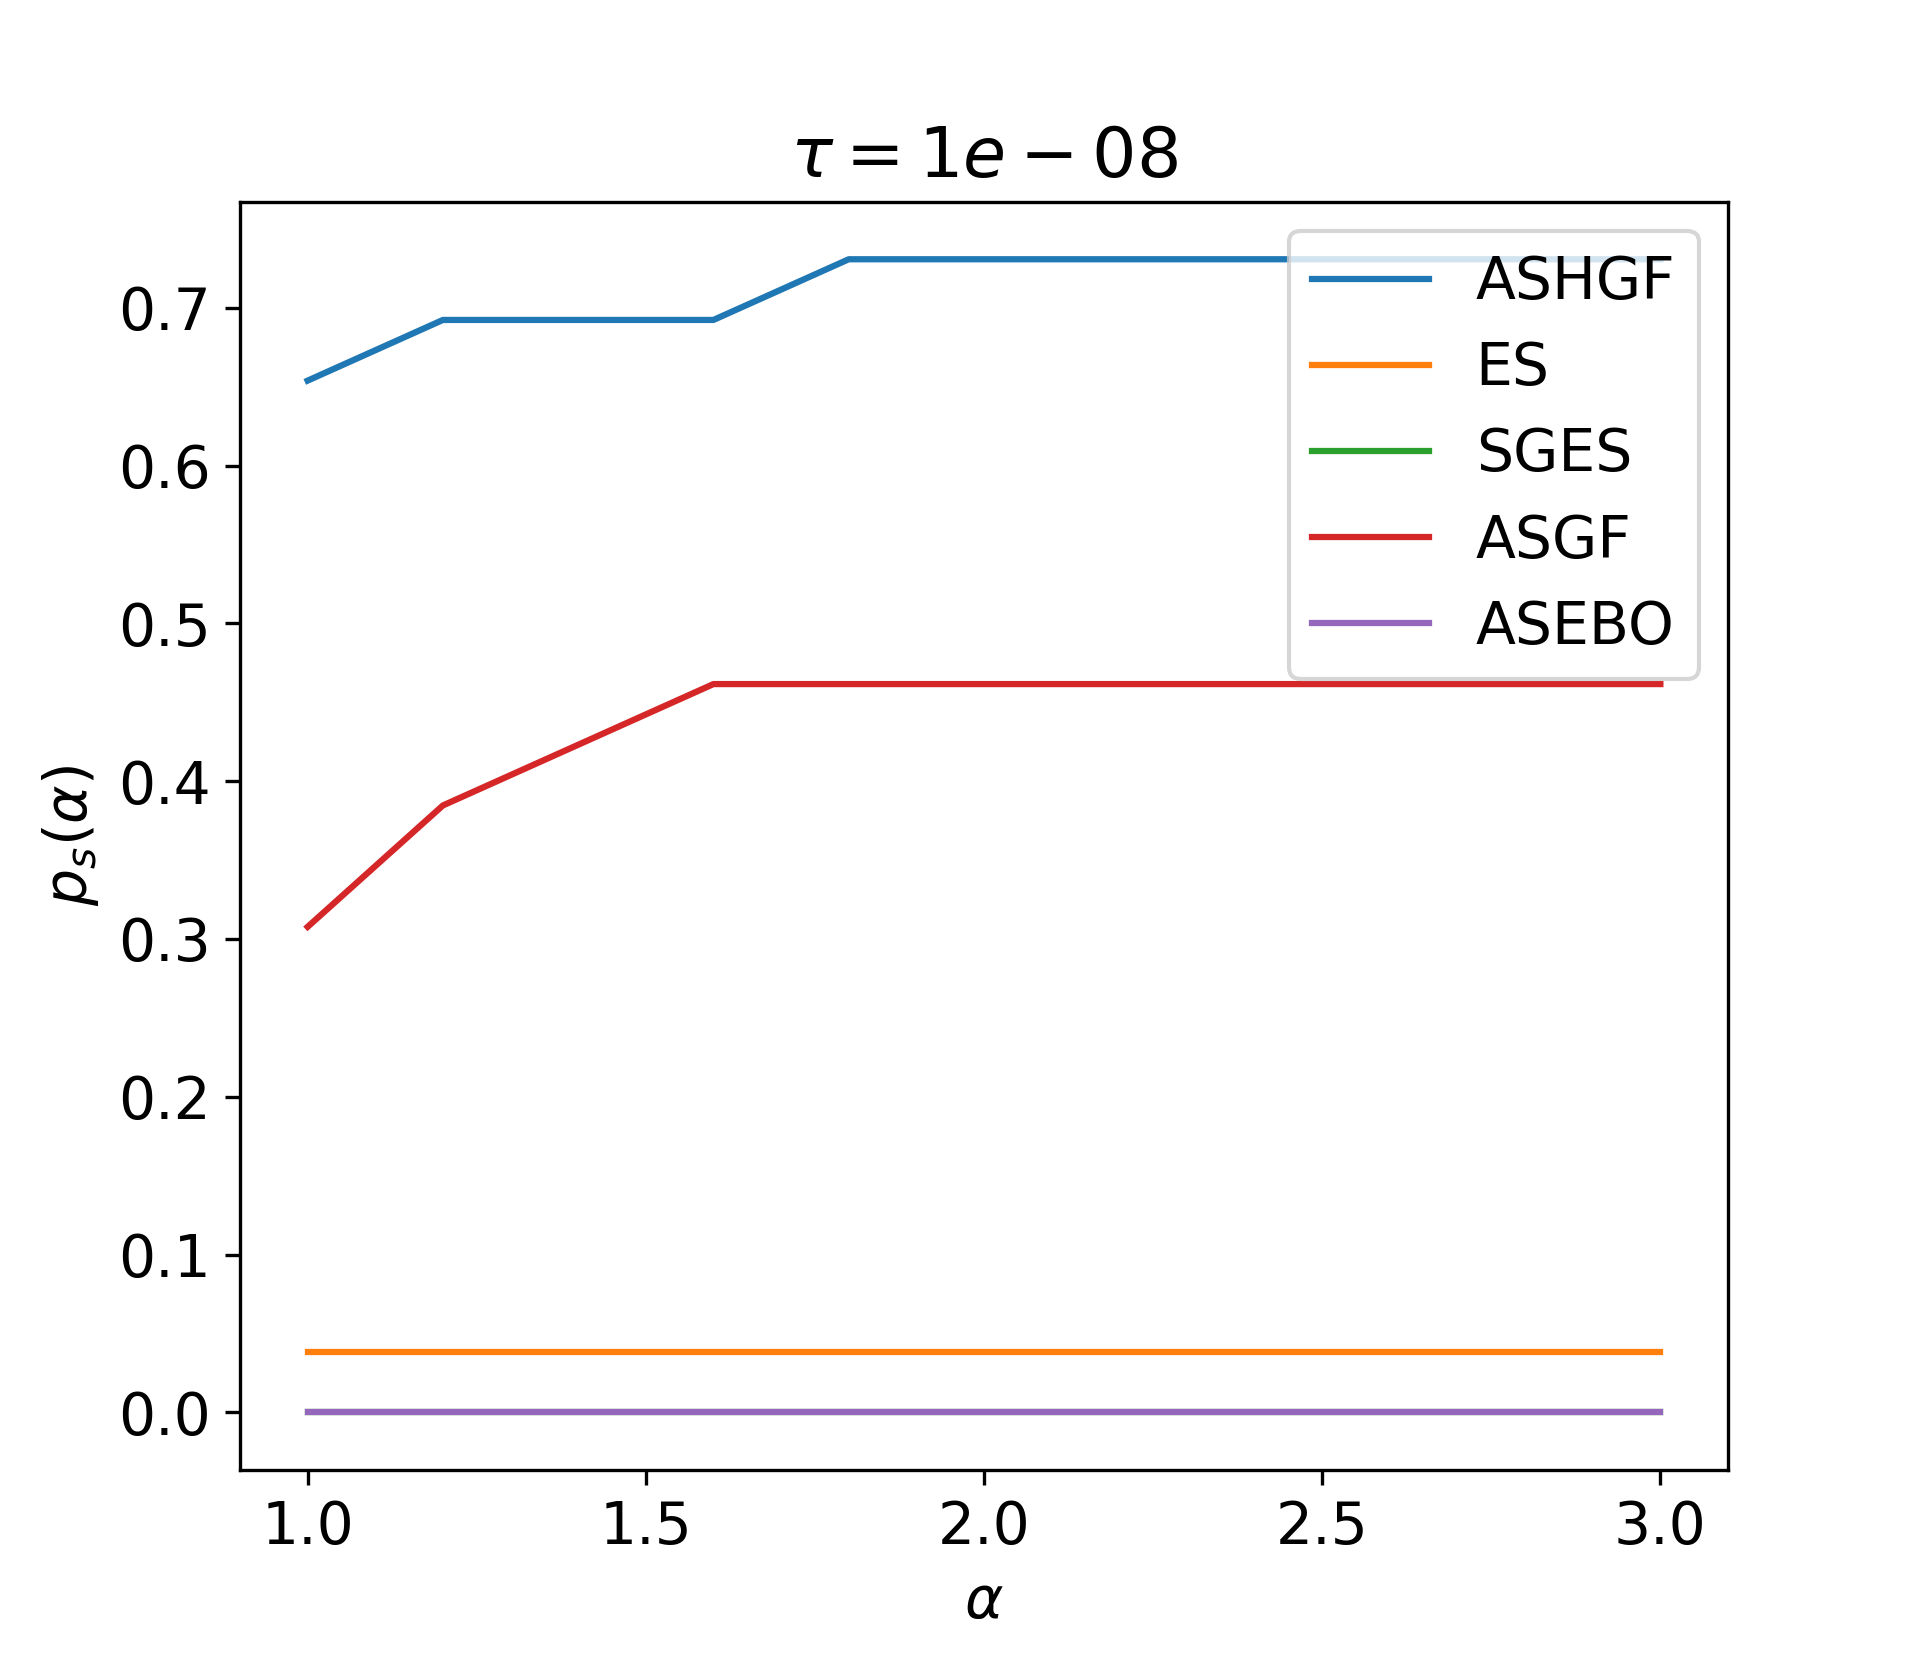
\includegraphics[width=1\textwidth]{figures/performance_profiles/100/performance_profile_100_100000_1e-08.png}
\end{subfigure}%
\begin{subfigure}{0.3\textwidth}
  \centering 
  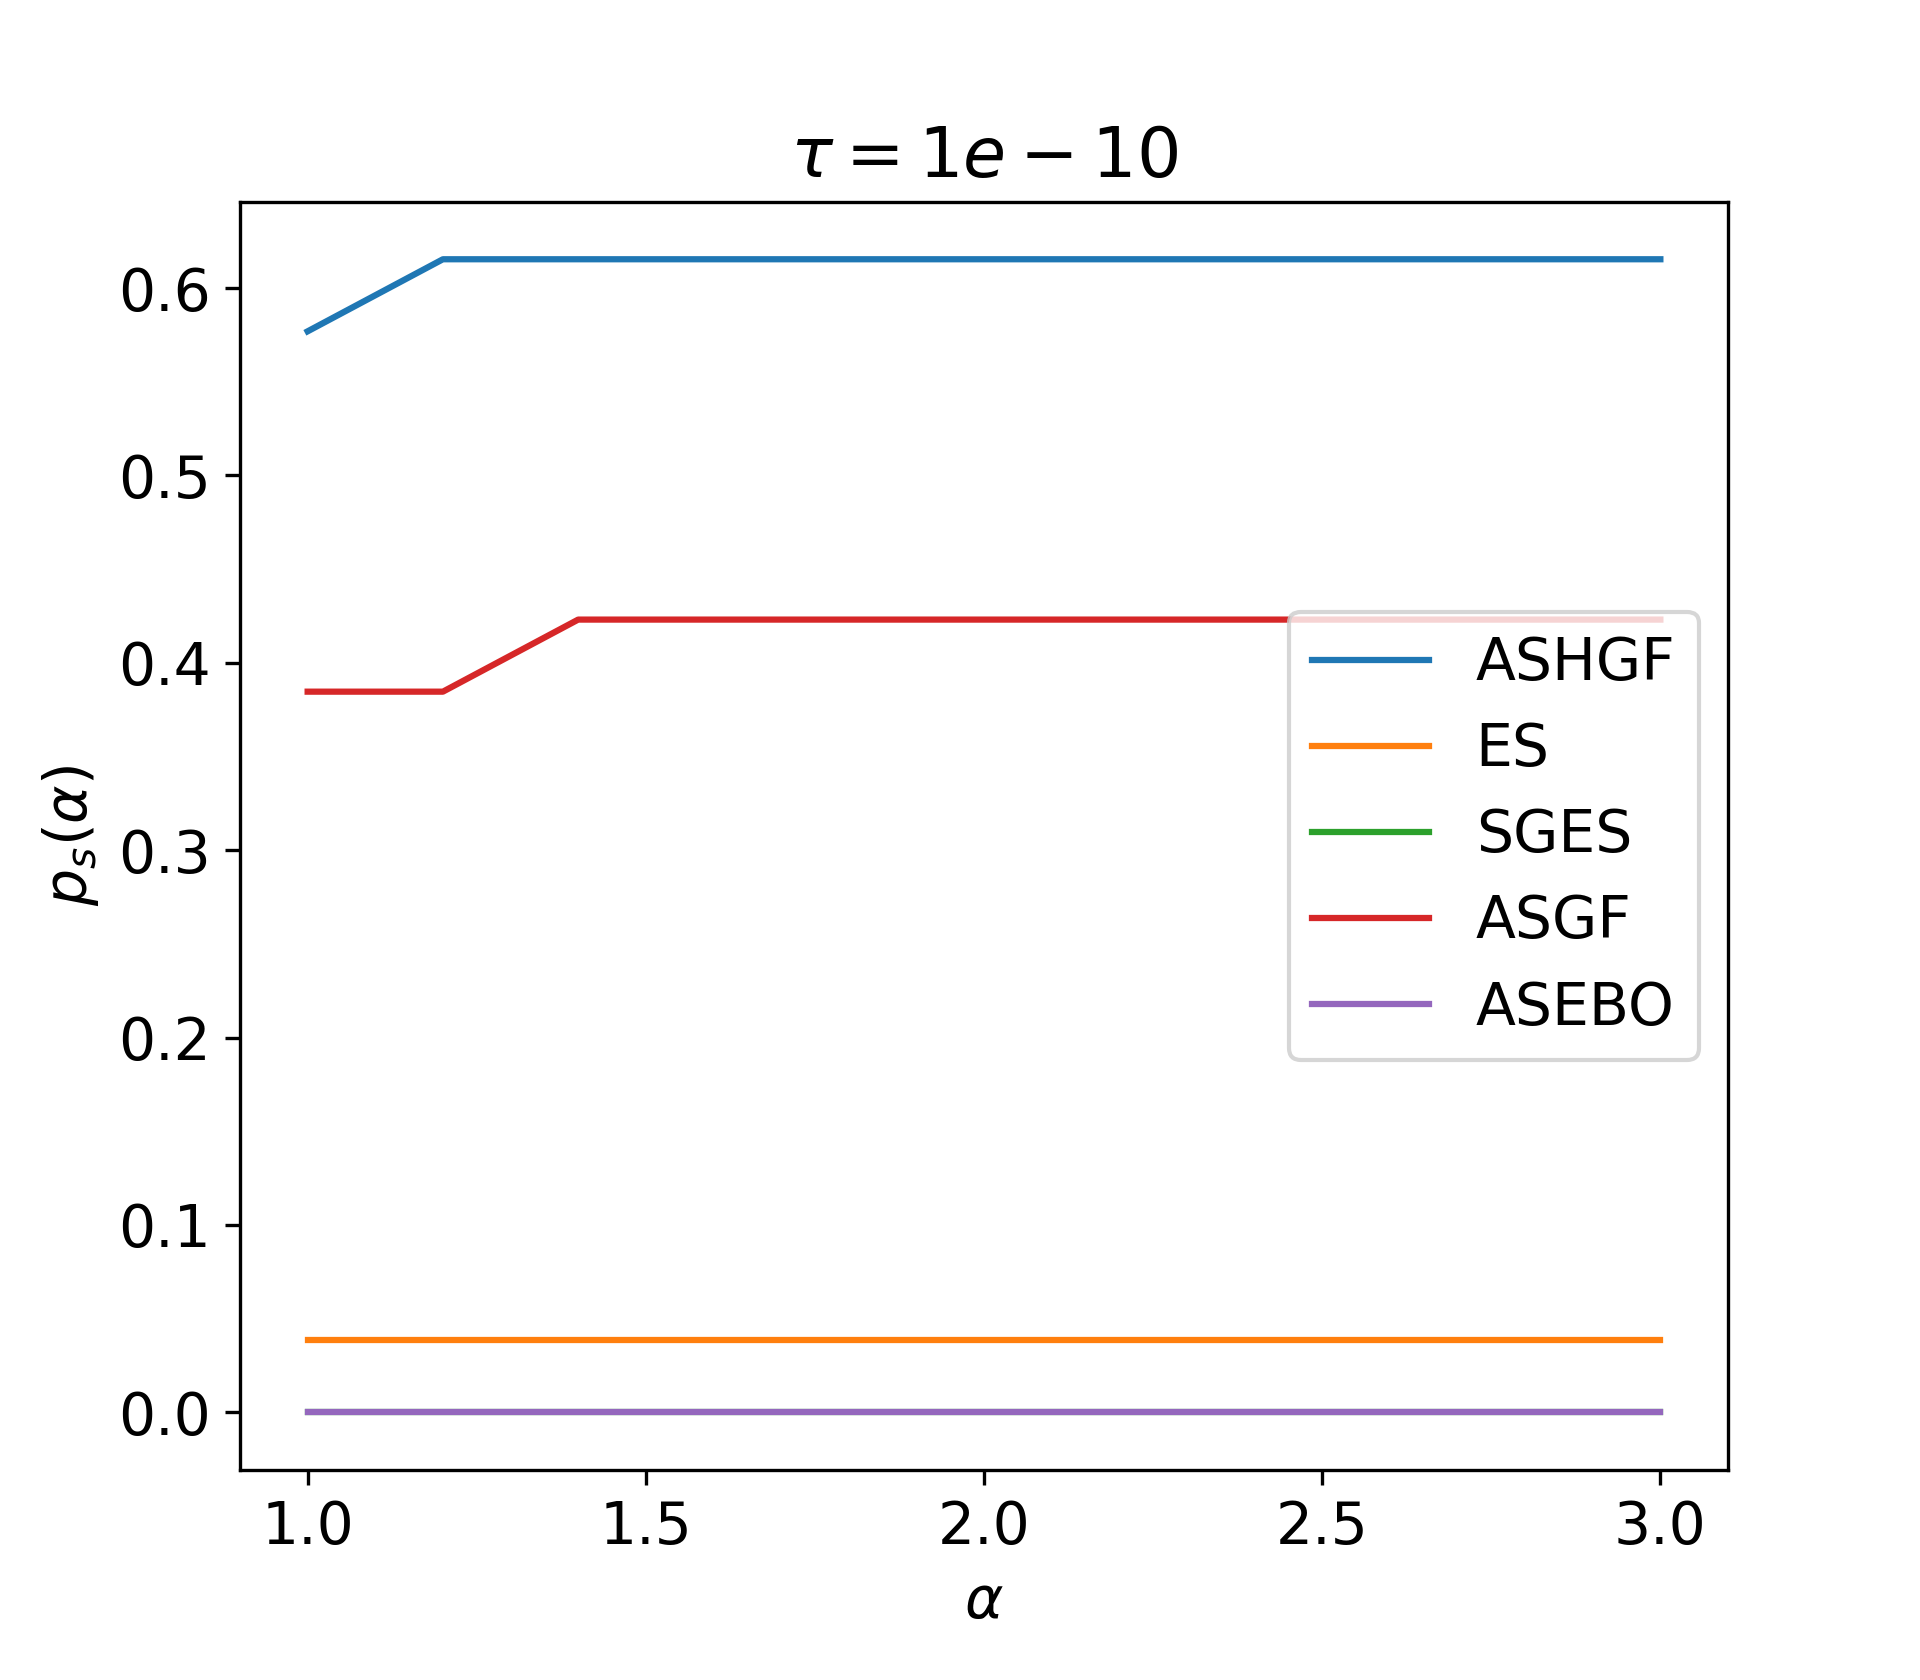
\includegraphics[width=1\textwidth]{figures/performance_profiles/100/performance_profile_100_100000_1e-10.png}
\end{subfigure}
\caption{Performance profiles with $\mu_L = 10^{5}$}
\label{PerformanceProfiles100Mu100000}
\end{figure}

\begin{figure}[H]
\centering
\begin{subfigure}{0.3\textwidth}
  \centering 
  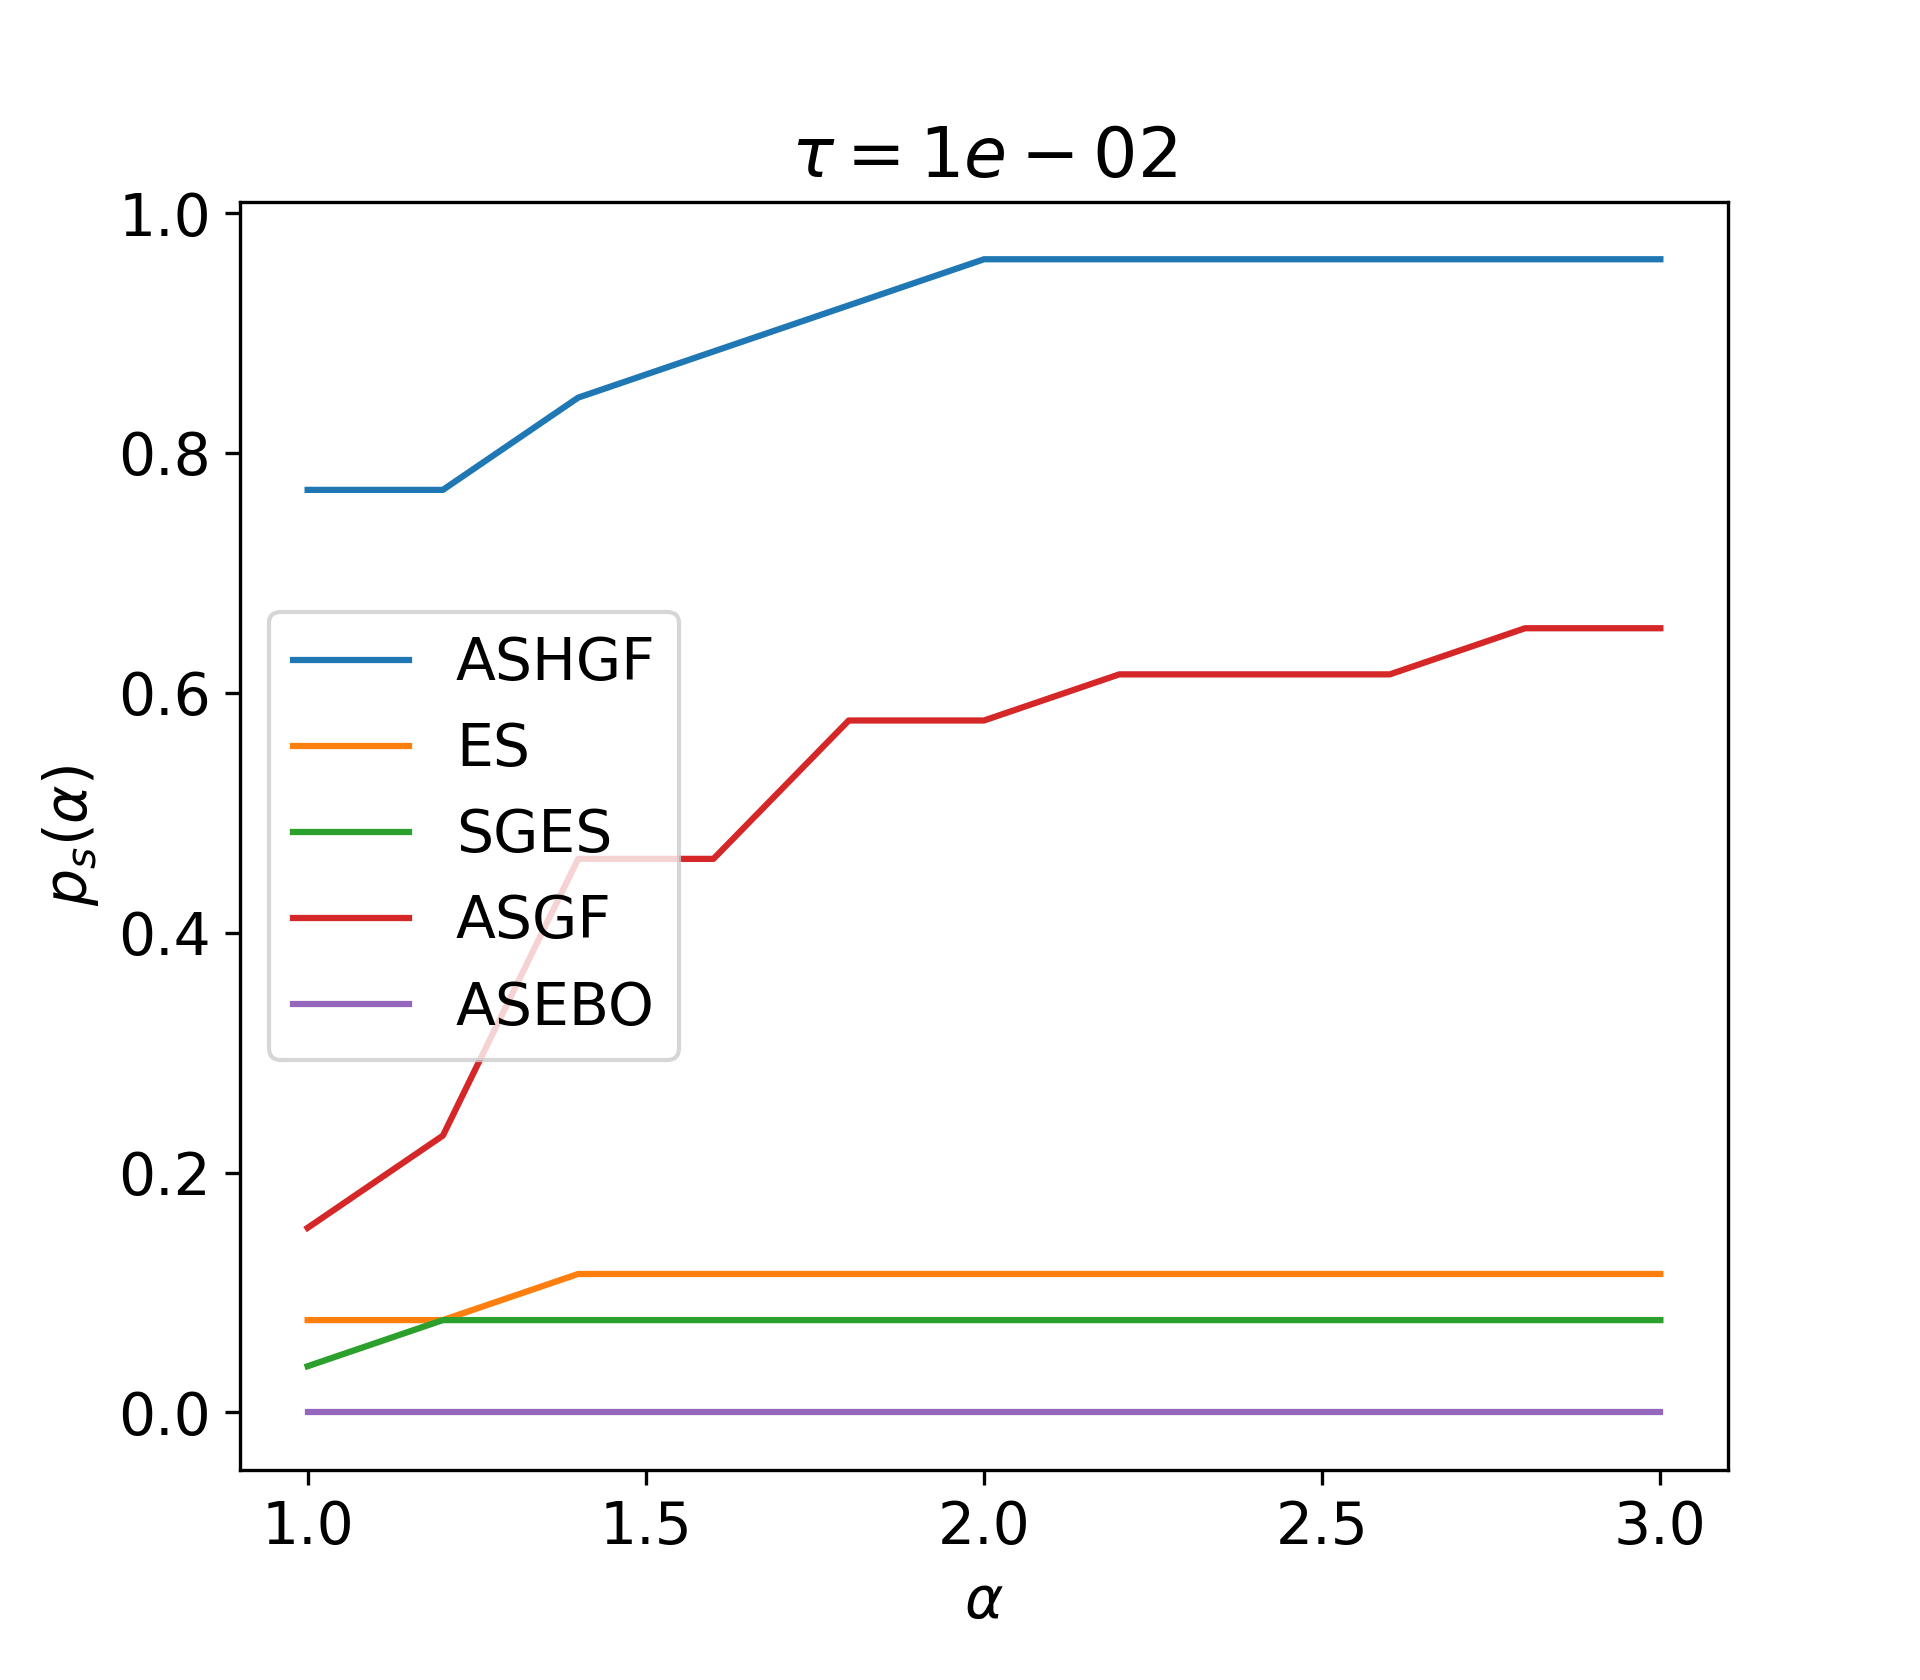
\includegraphics[width=1\textwidth]{figures/performance_profiles/100/performance_profile_100_1000000_1e-02.png}
\end{subfigure}%
\begin{subfigure}{0.3\textwidth}
  \centering 
  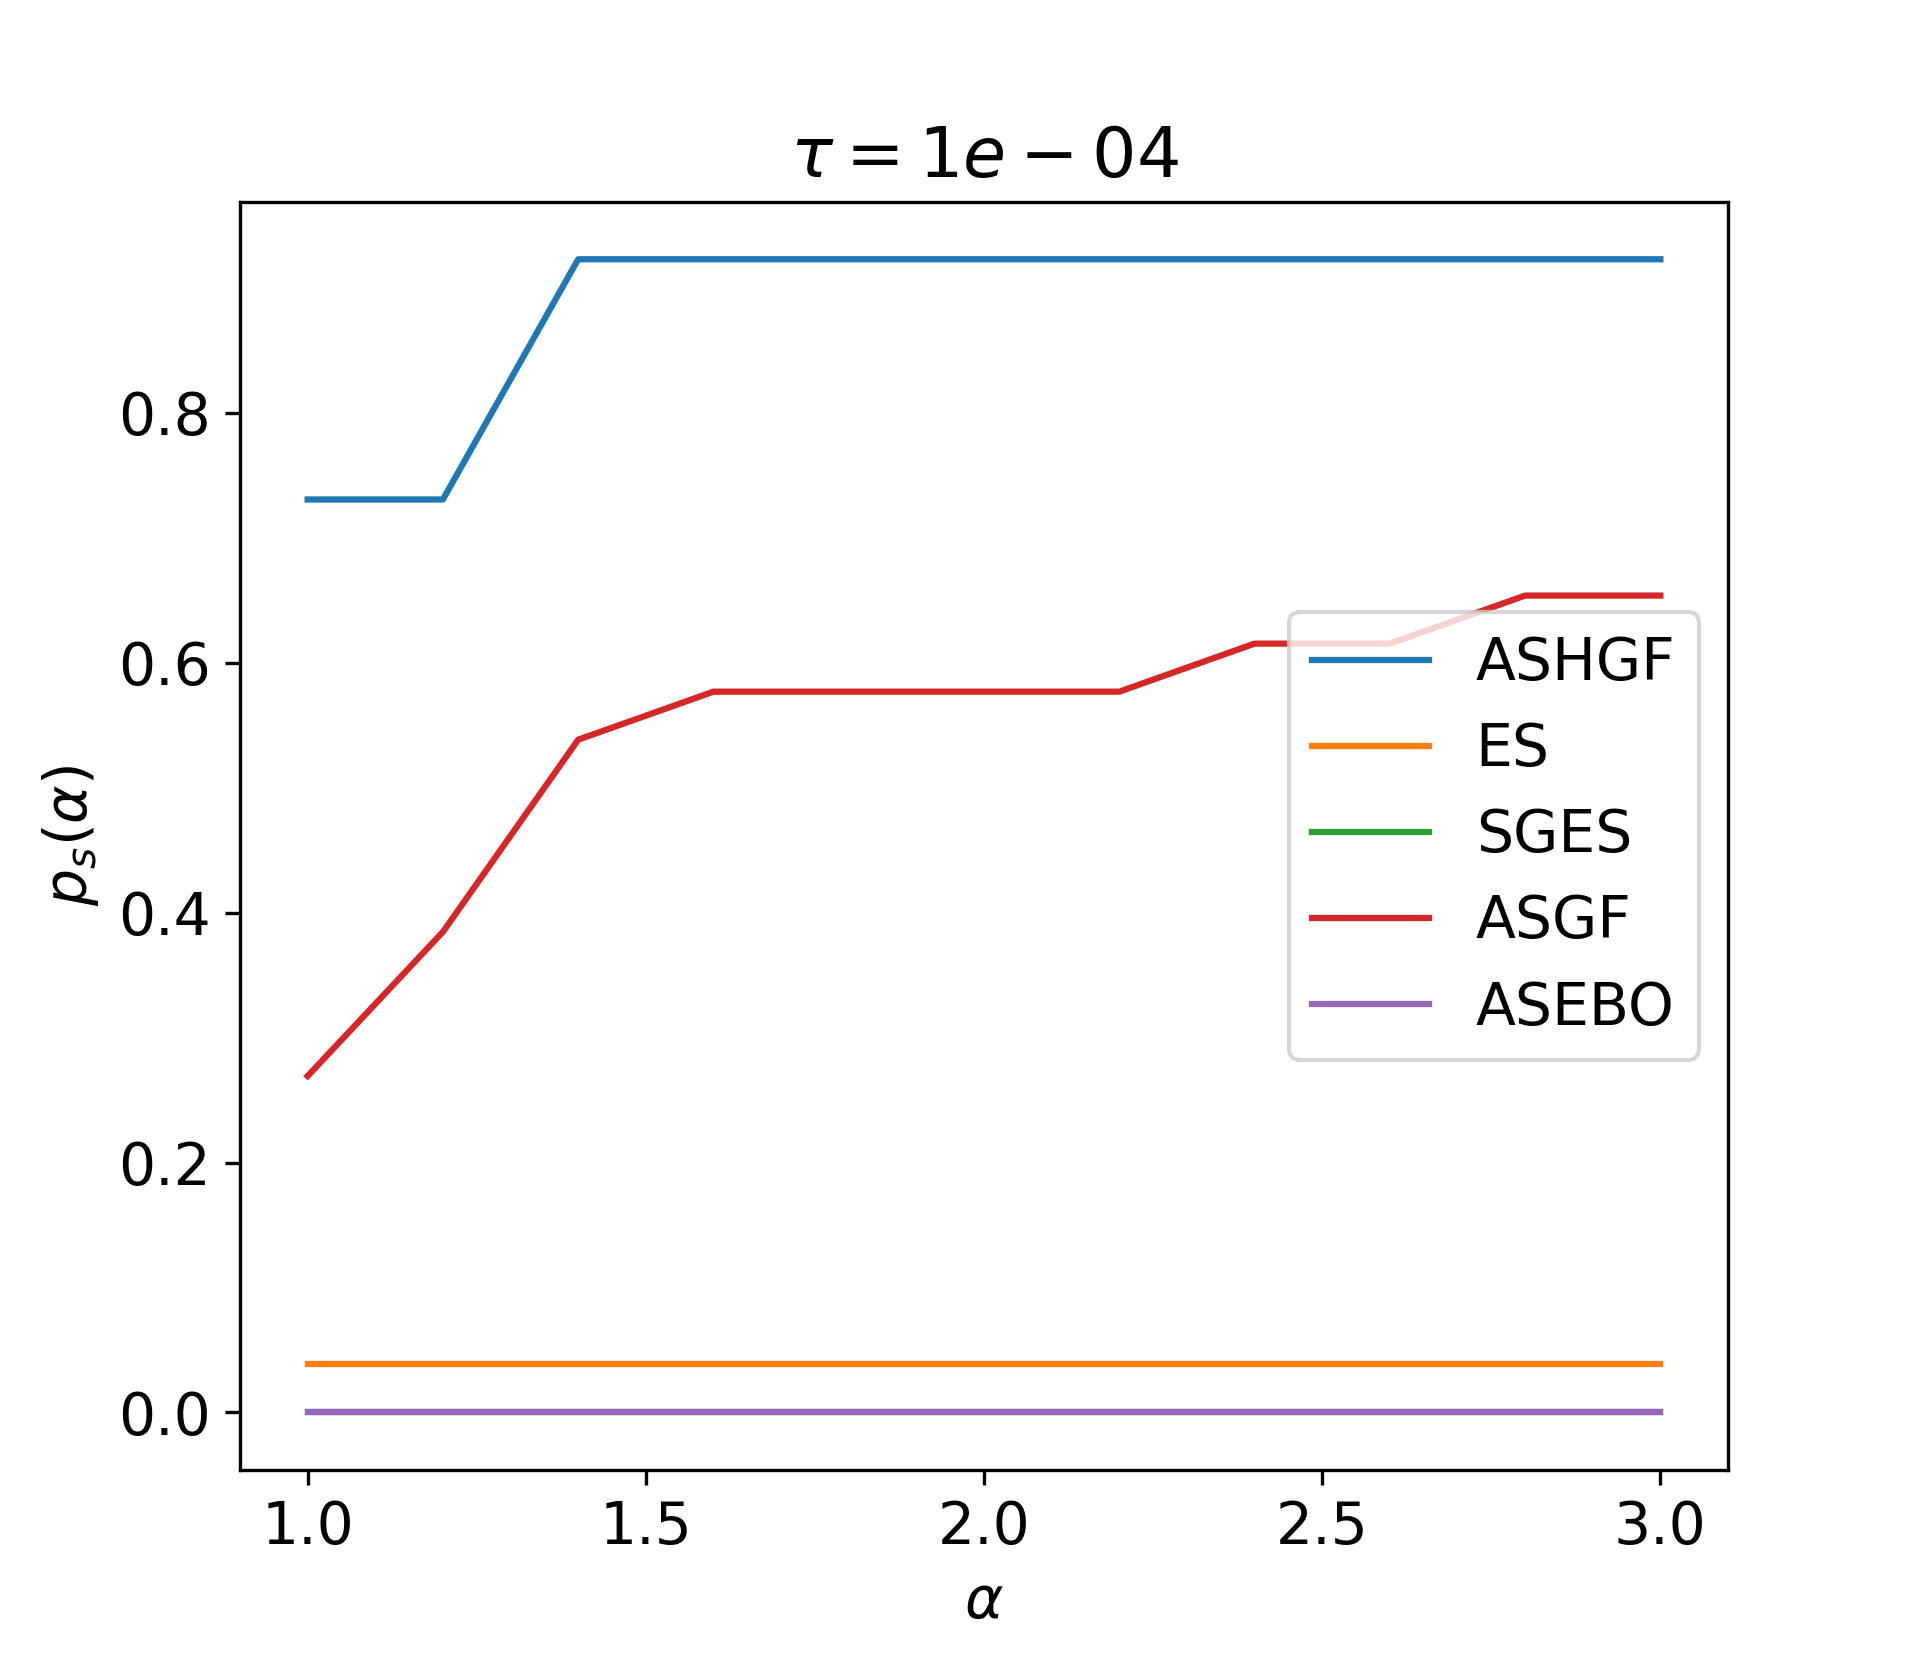
\includegraphics[width=1\textwidth]{figures/performance_profiles/100/performance_profile_100_1000000_1e-04.png}
\end{subfigure}
\begin{subfigure}{0.3\textwidth}
  \centering 
  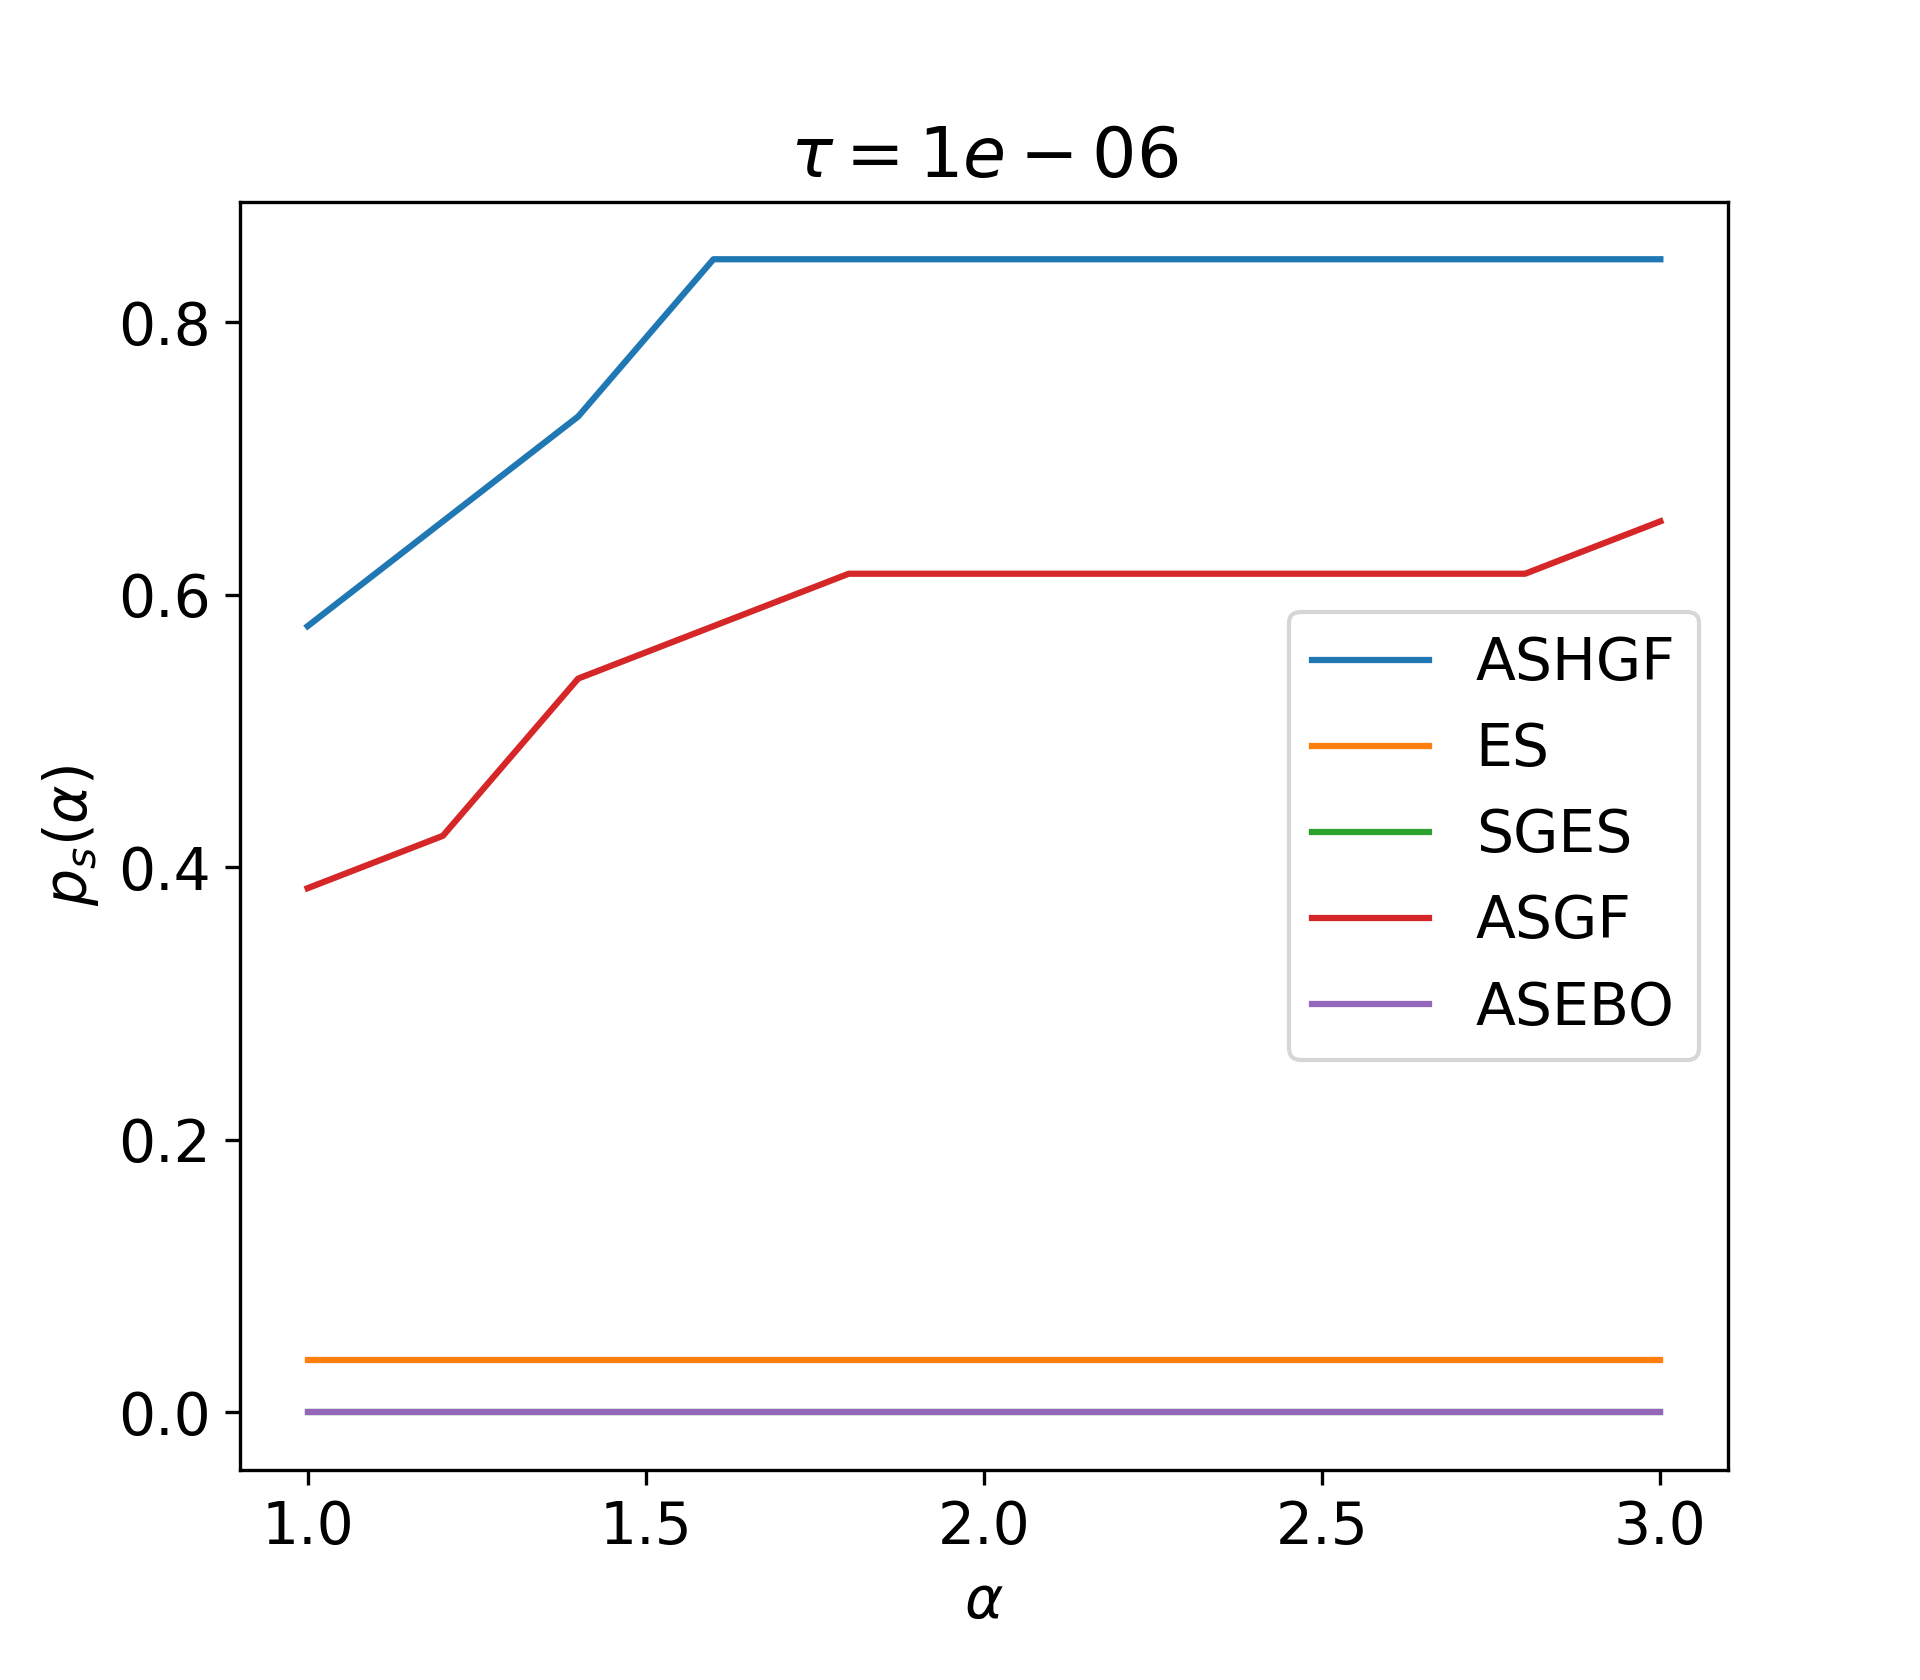
\includegraphics[width=1\textwidth]{figures/performance_profiles/100/performance_profile_100_1000000_1e-06.png}
\end{subfigure}
\centering
\begin{subfigure}{0.3\textwidth}
  \centering 
  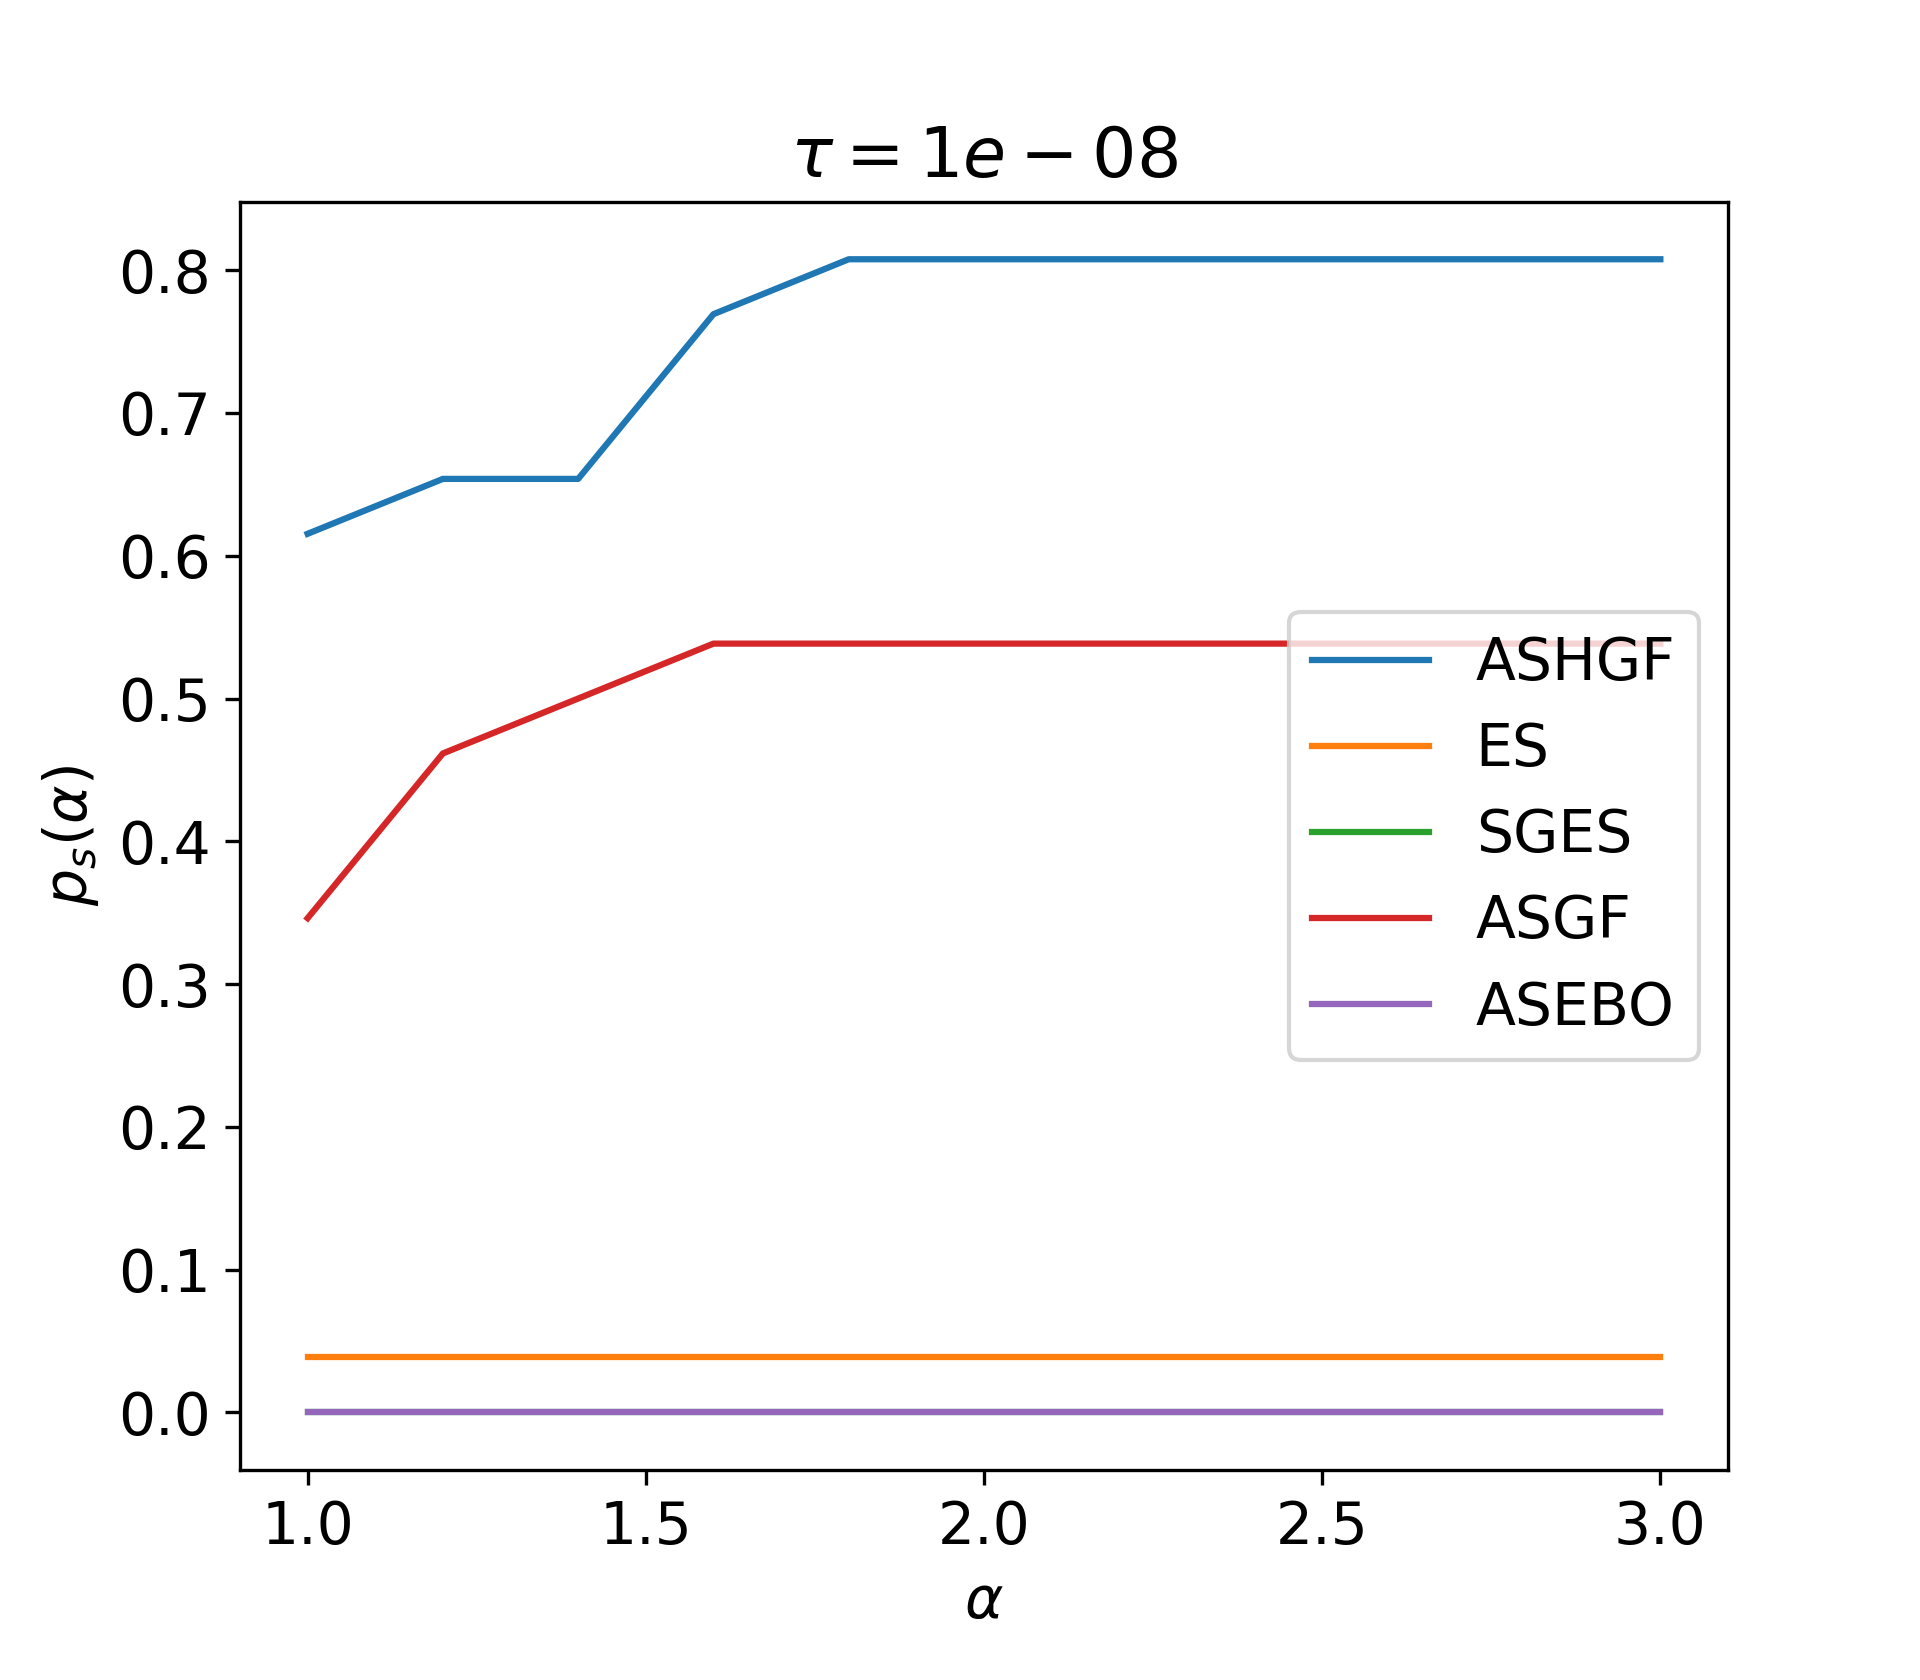
\includegraphics[width=1\textwidth]{figures/performance_profiles/100/performance_profile_100_1000000_1e-08.png}
\end{subfigure}%
\begin{subfigure}{0.3\textwidth}
  \centering 
  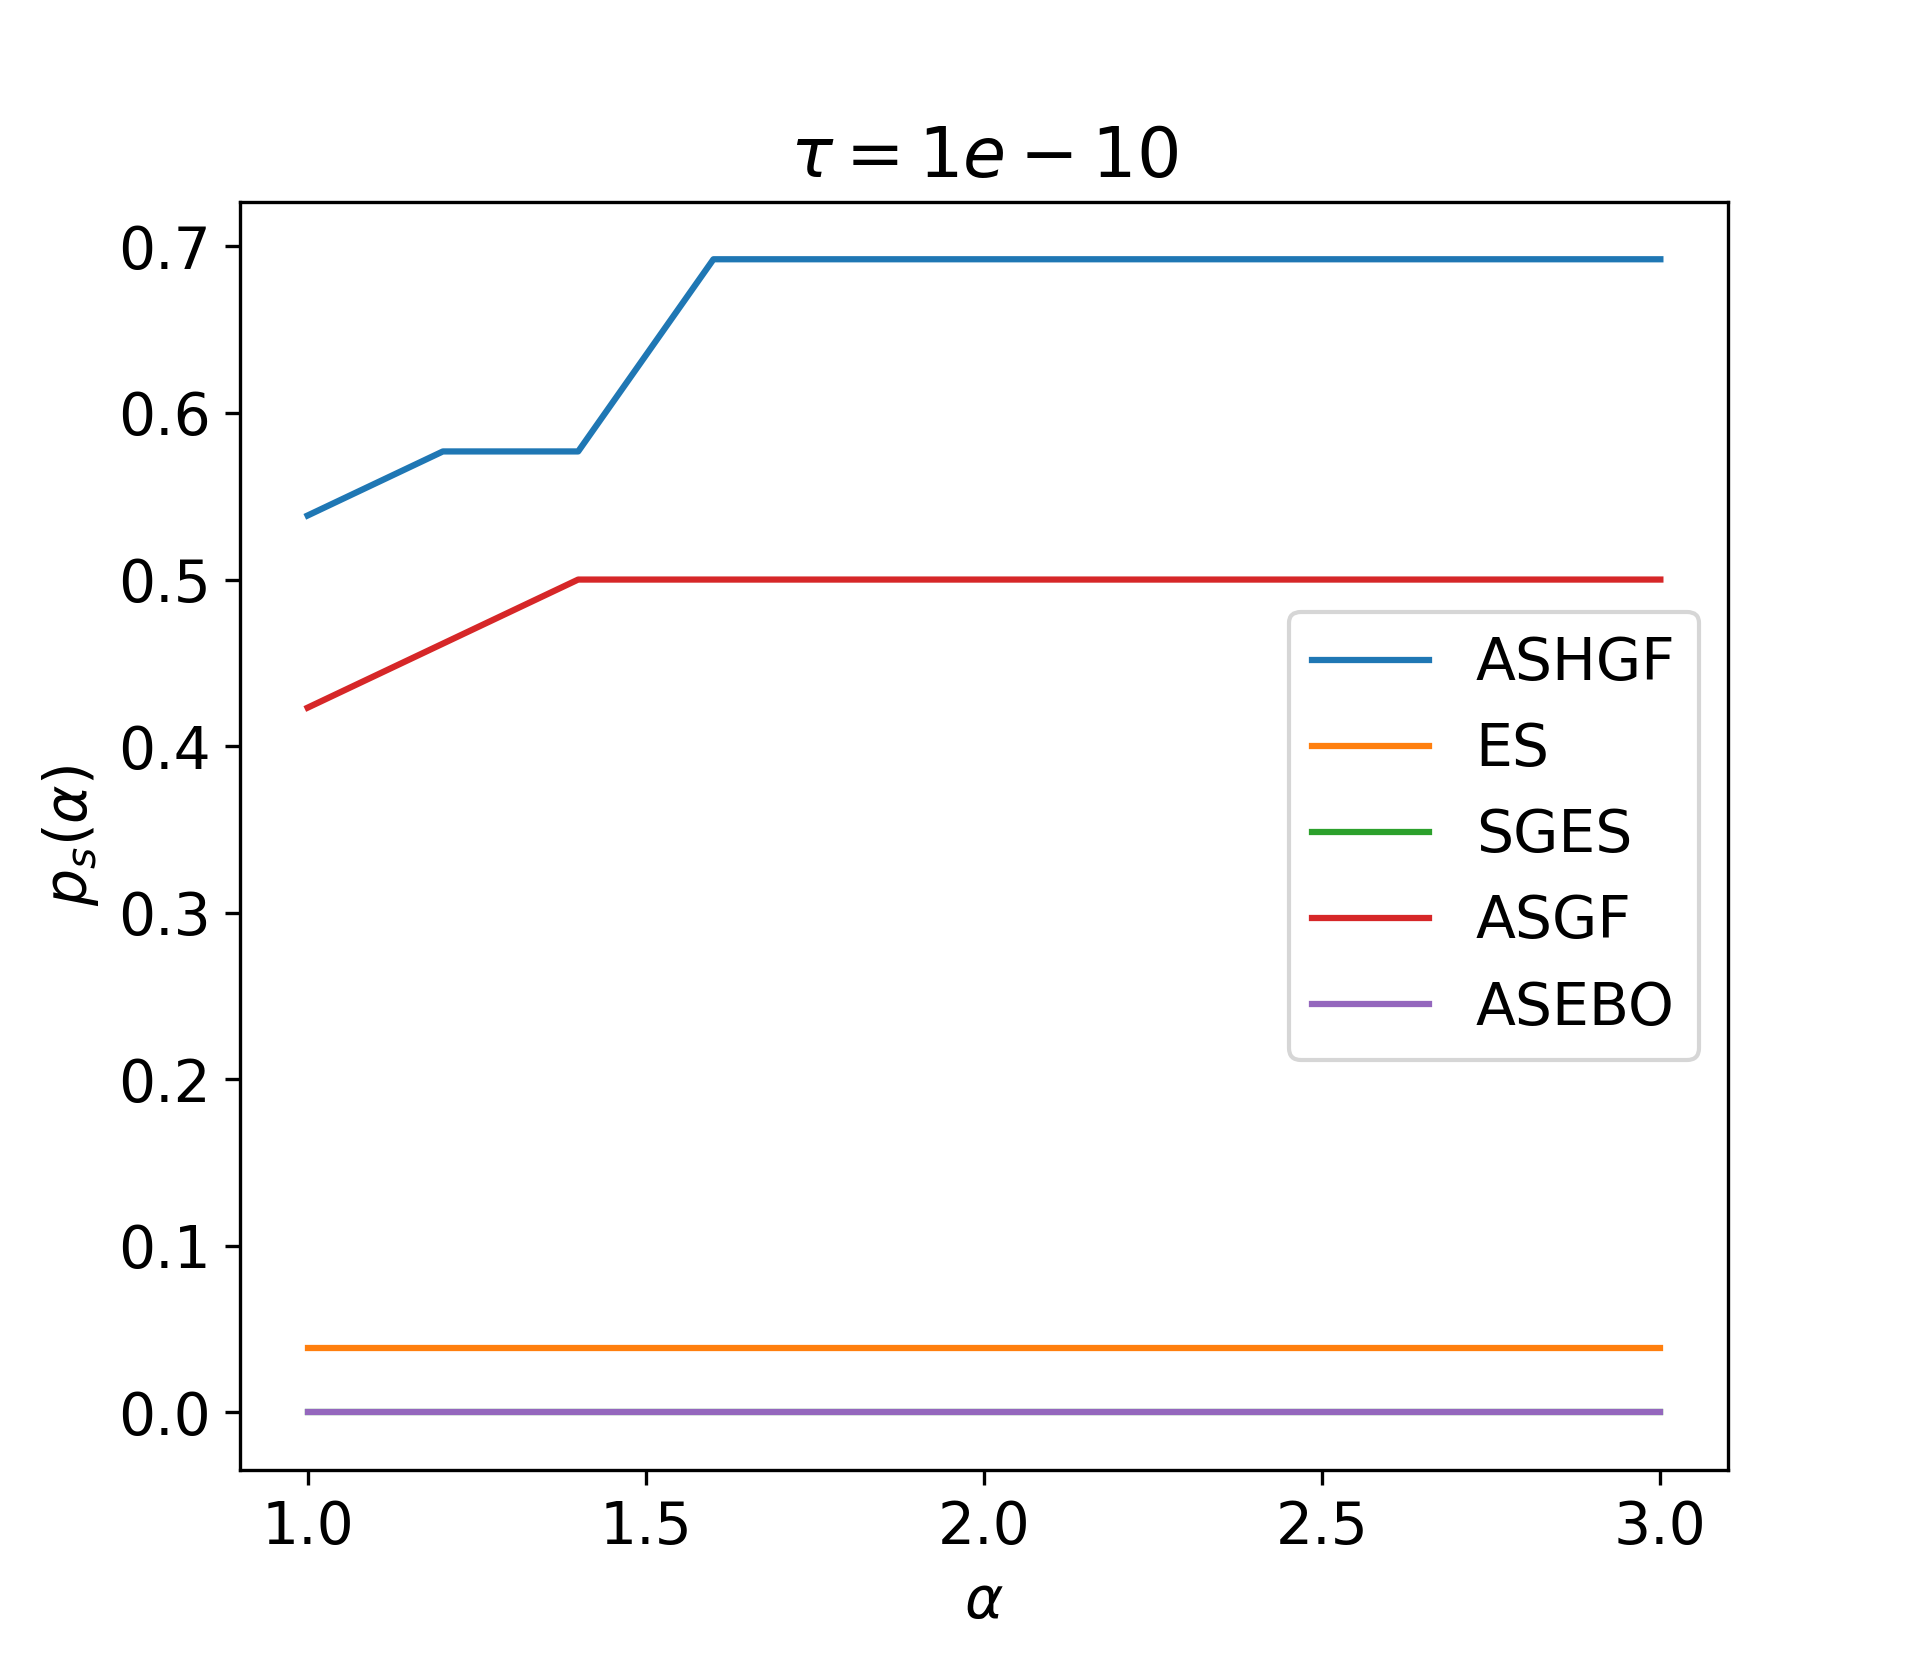
\includegraphics[width=1\textwidth]{figures/performance_profiles/100/performance_profile_100_1000000_1e-10.png}
\end{subfigure}
\caption{Performance profiles with $\mu_L = 10^{6}$}
\label{PerformanceProfiles100Mu1000000}
\end{figure}

\begin{figure}[H]
\centering
\begin{subfigure}{0.3\textwidth}
  \centering 
  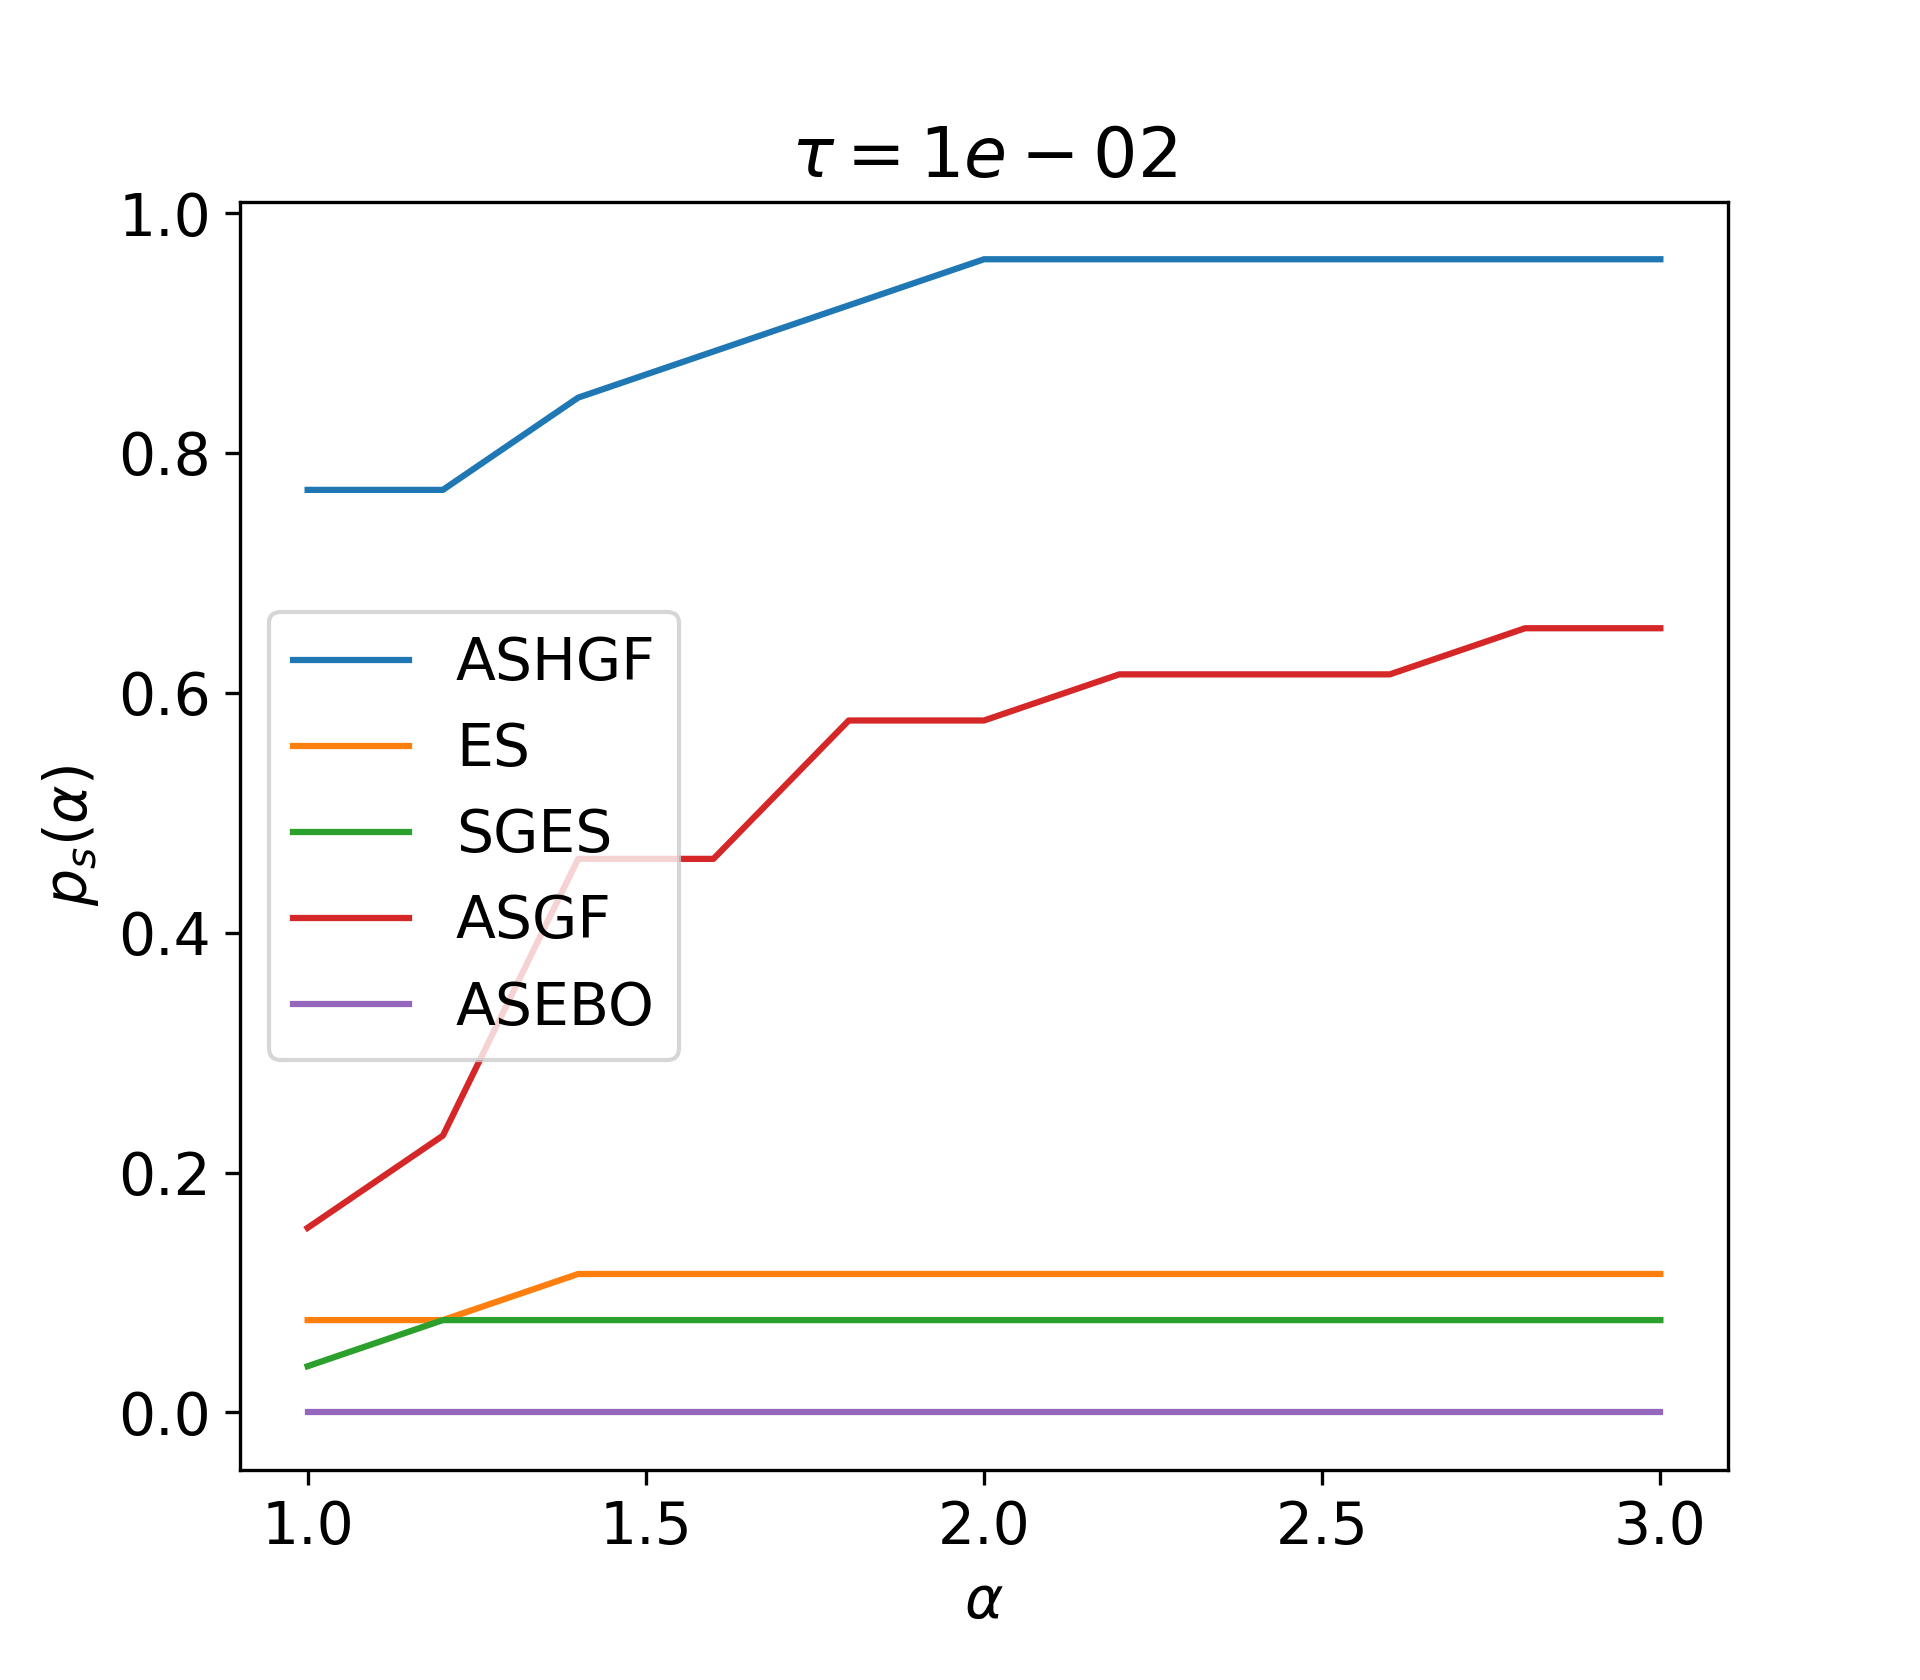
\includegraphics[width=1\textwidth]{figures/performance_profiles/100/performance_profile_100_10000000_1e-02.png}
\end{subfigure}%
\begin{subfigure}{0.3\textwidth}
  \centering 
  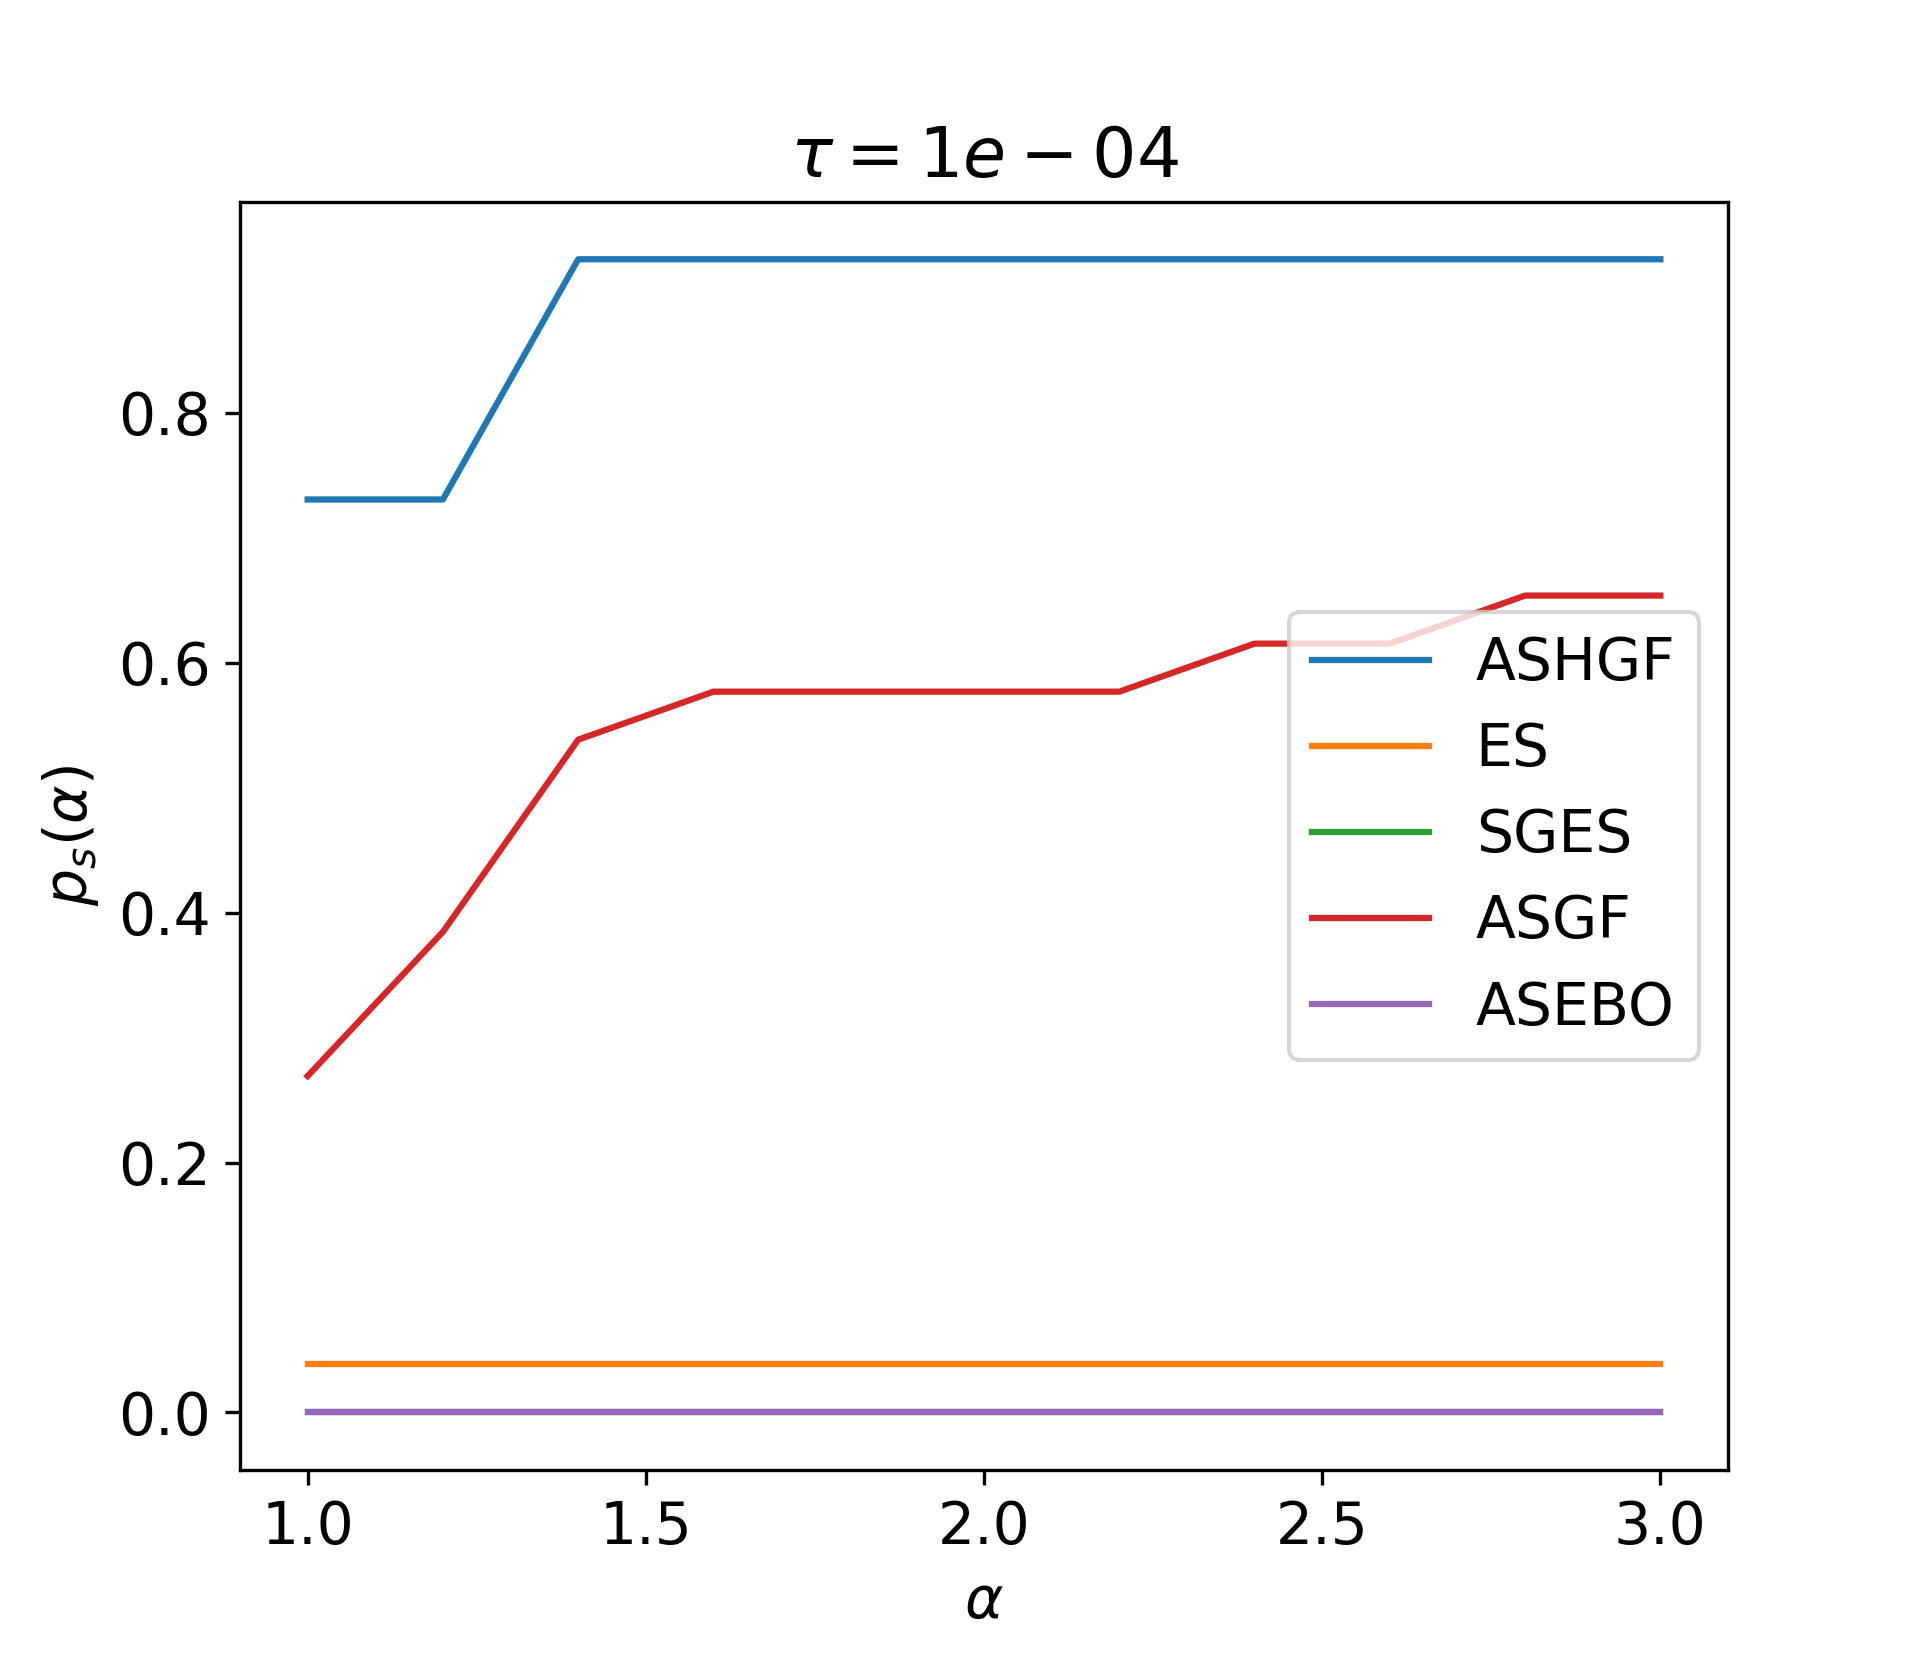
\includegraphics[width=1\textwidth]{figures/performance_profiles/100/performance_profile_100_10000000_1e-04.png}
\end{subfigure}
\begin{subfigure}{0.3\textwidth}
  \centering 
  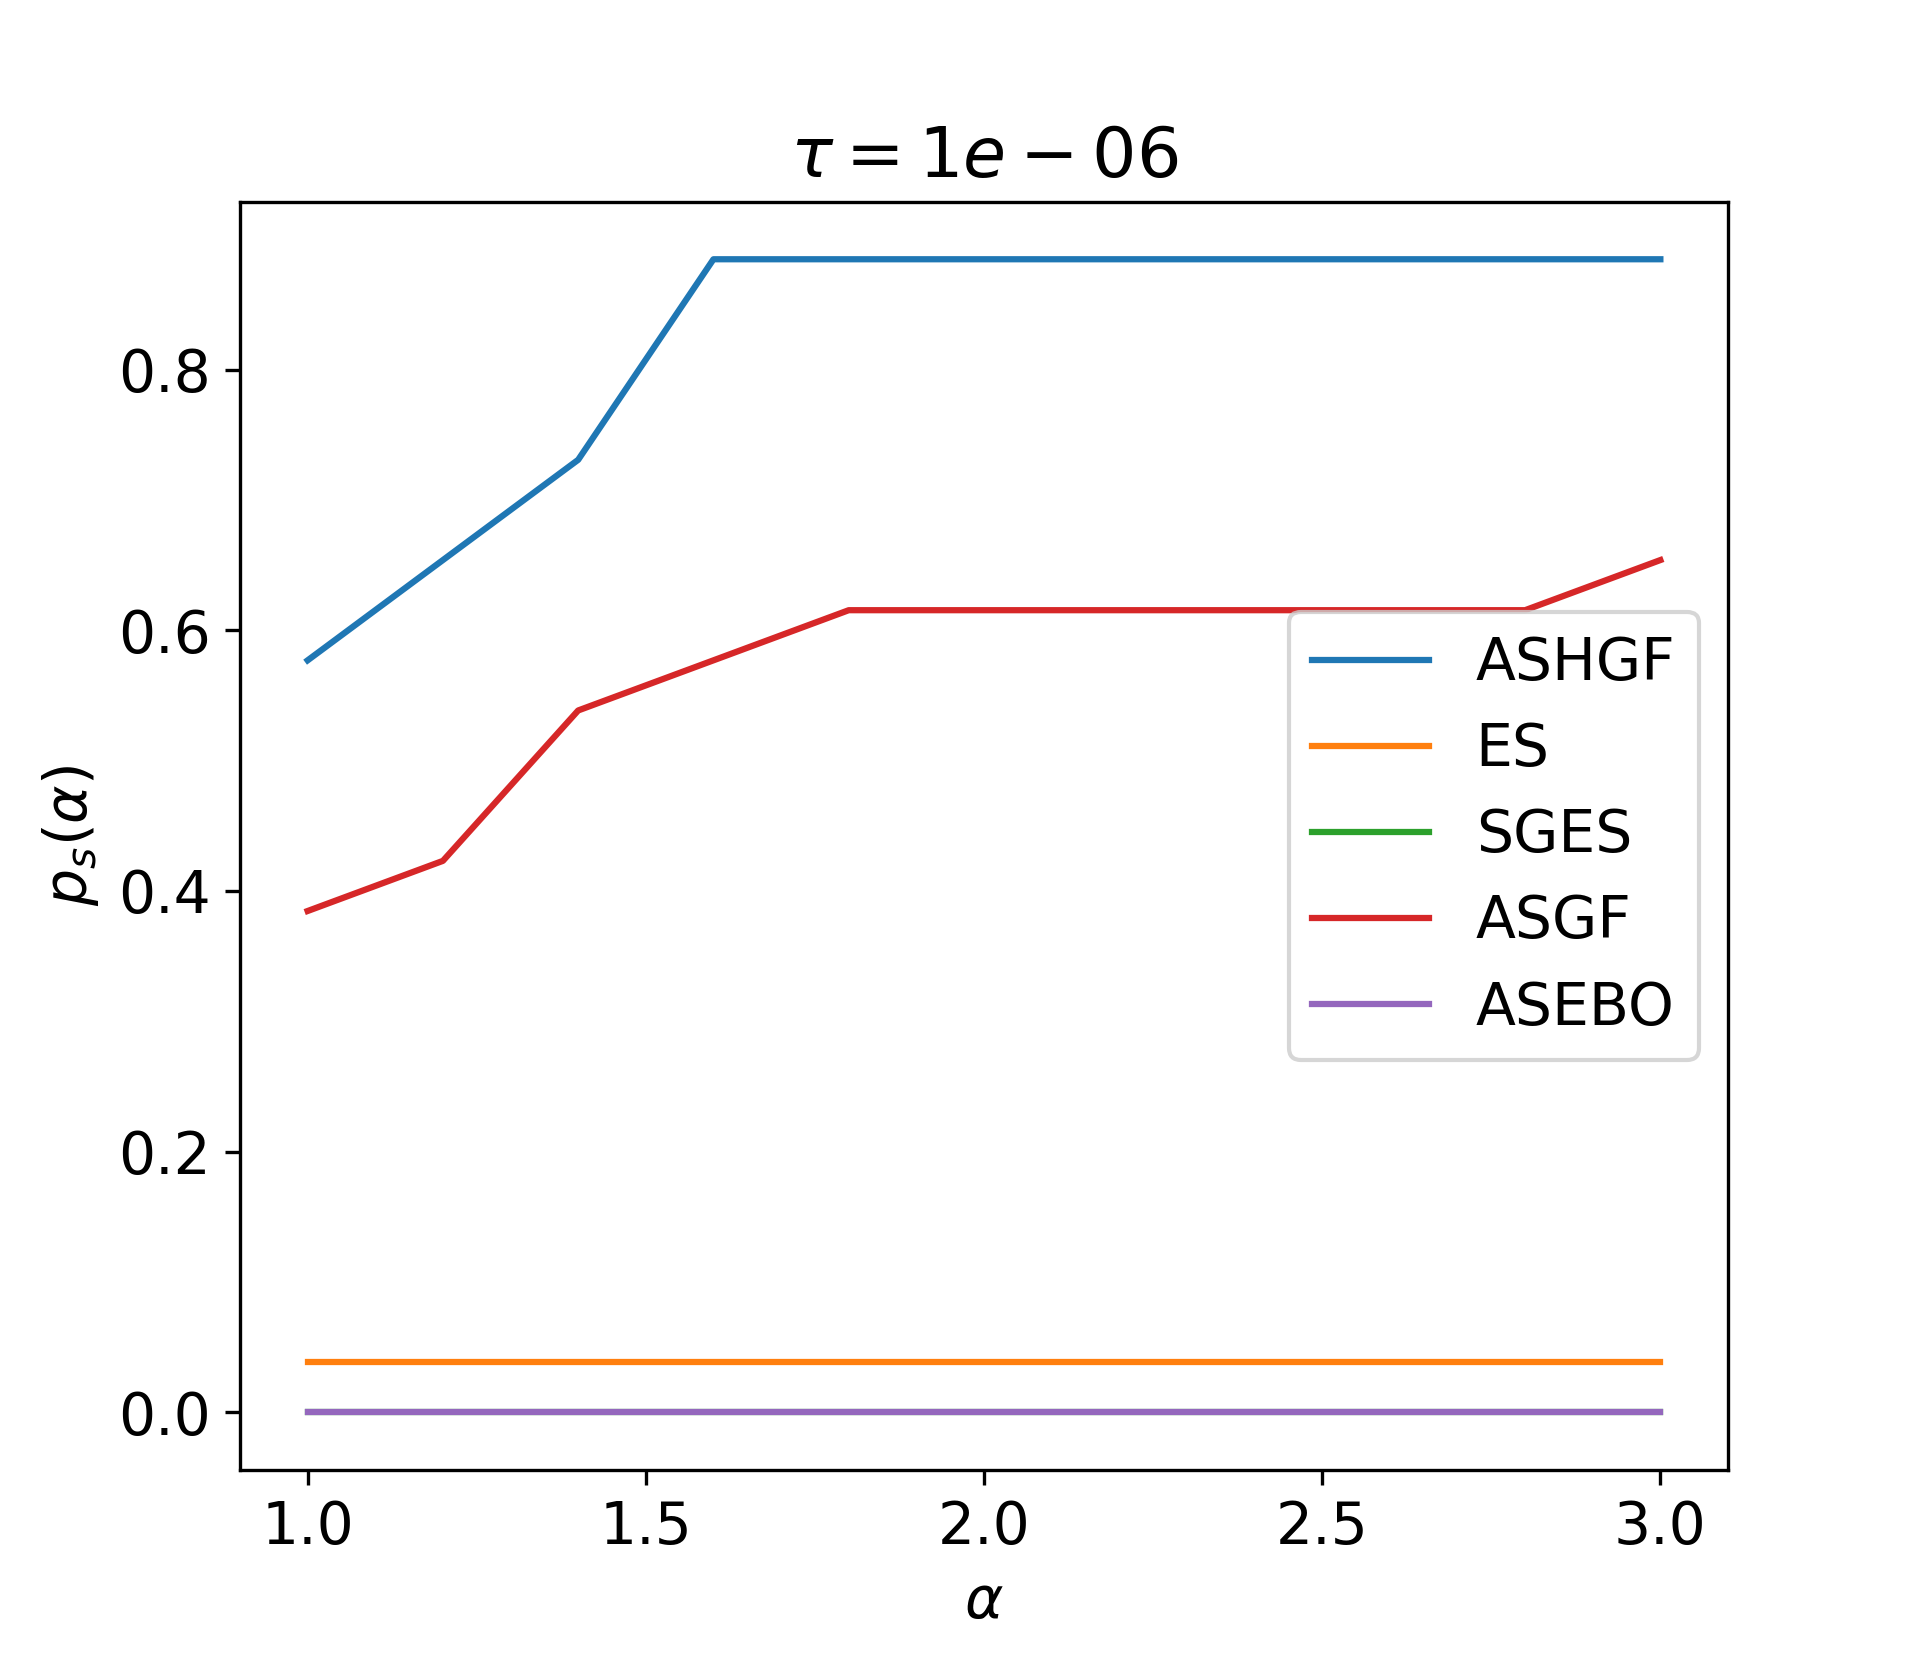
\includegraphics[width=1\textwidth]{figures/performance_profiles/100/performance_profile_100_10000000_1e-06.png}
\end{subfigure}
\centering
\begin{subfigure}{0.3\textwidth}
  \centering 
  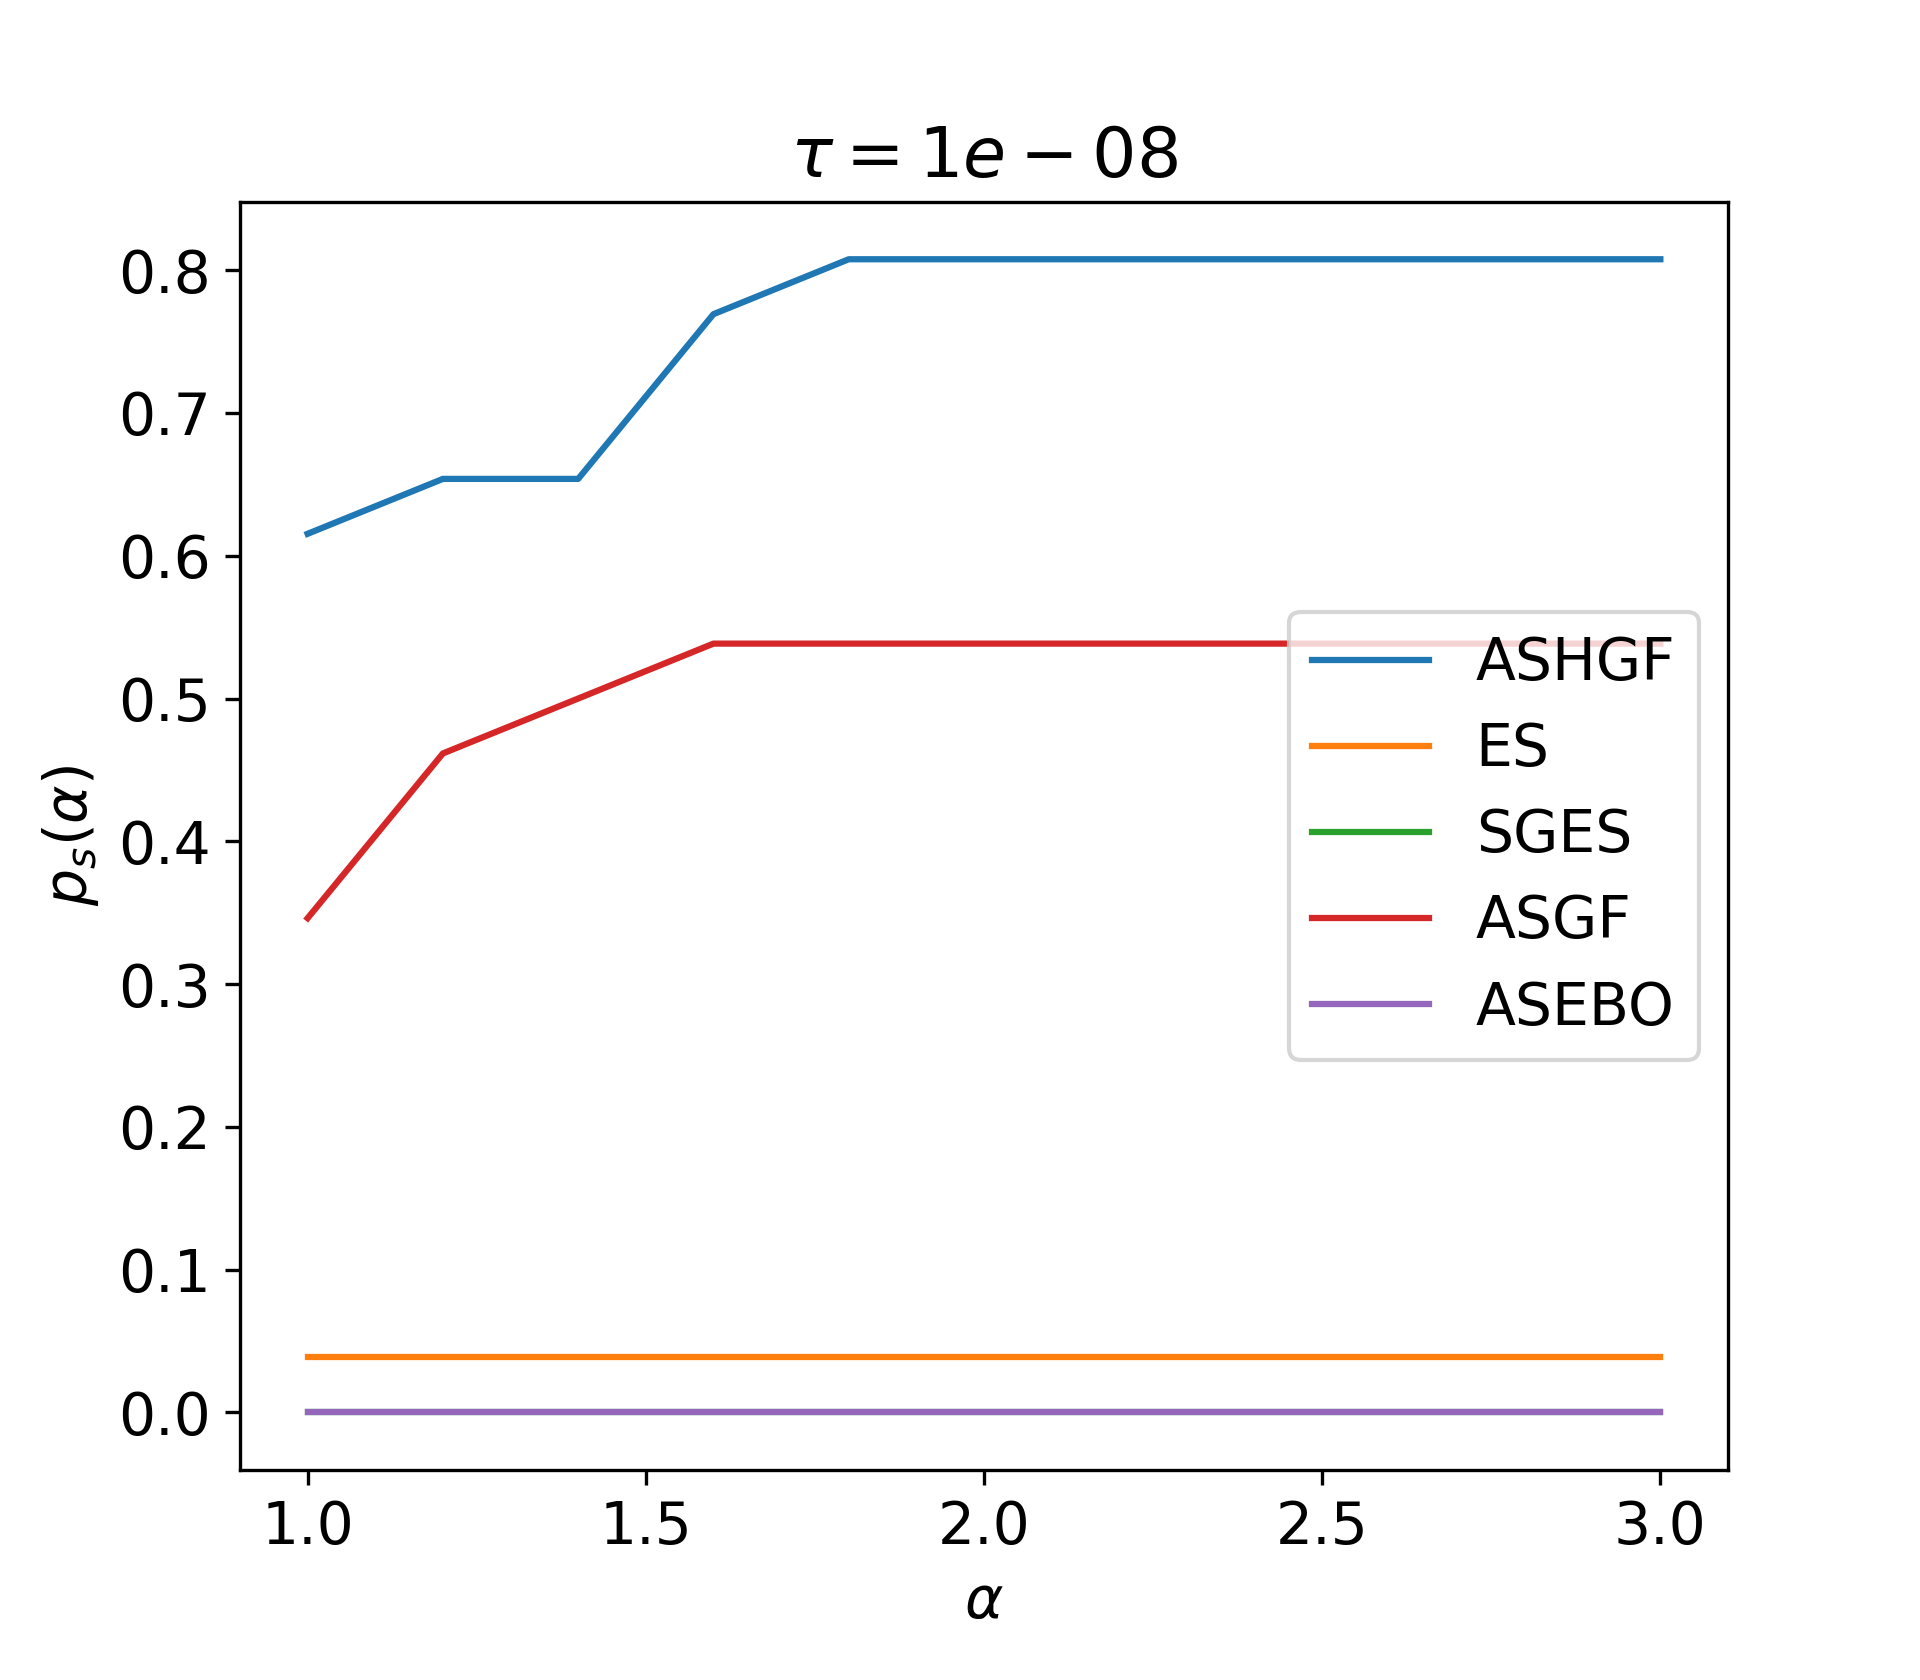
\includegraphics[width=1\textwidth]{figures/performance_profiles/100/performance_profile_100_10000000_1e-08.png}
\end{subfigure}%
\begin{subfigure}{0.3\textwidth}
  \centering 
  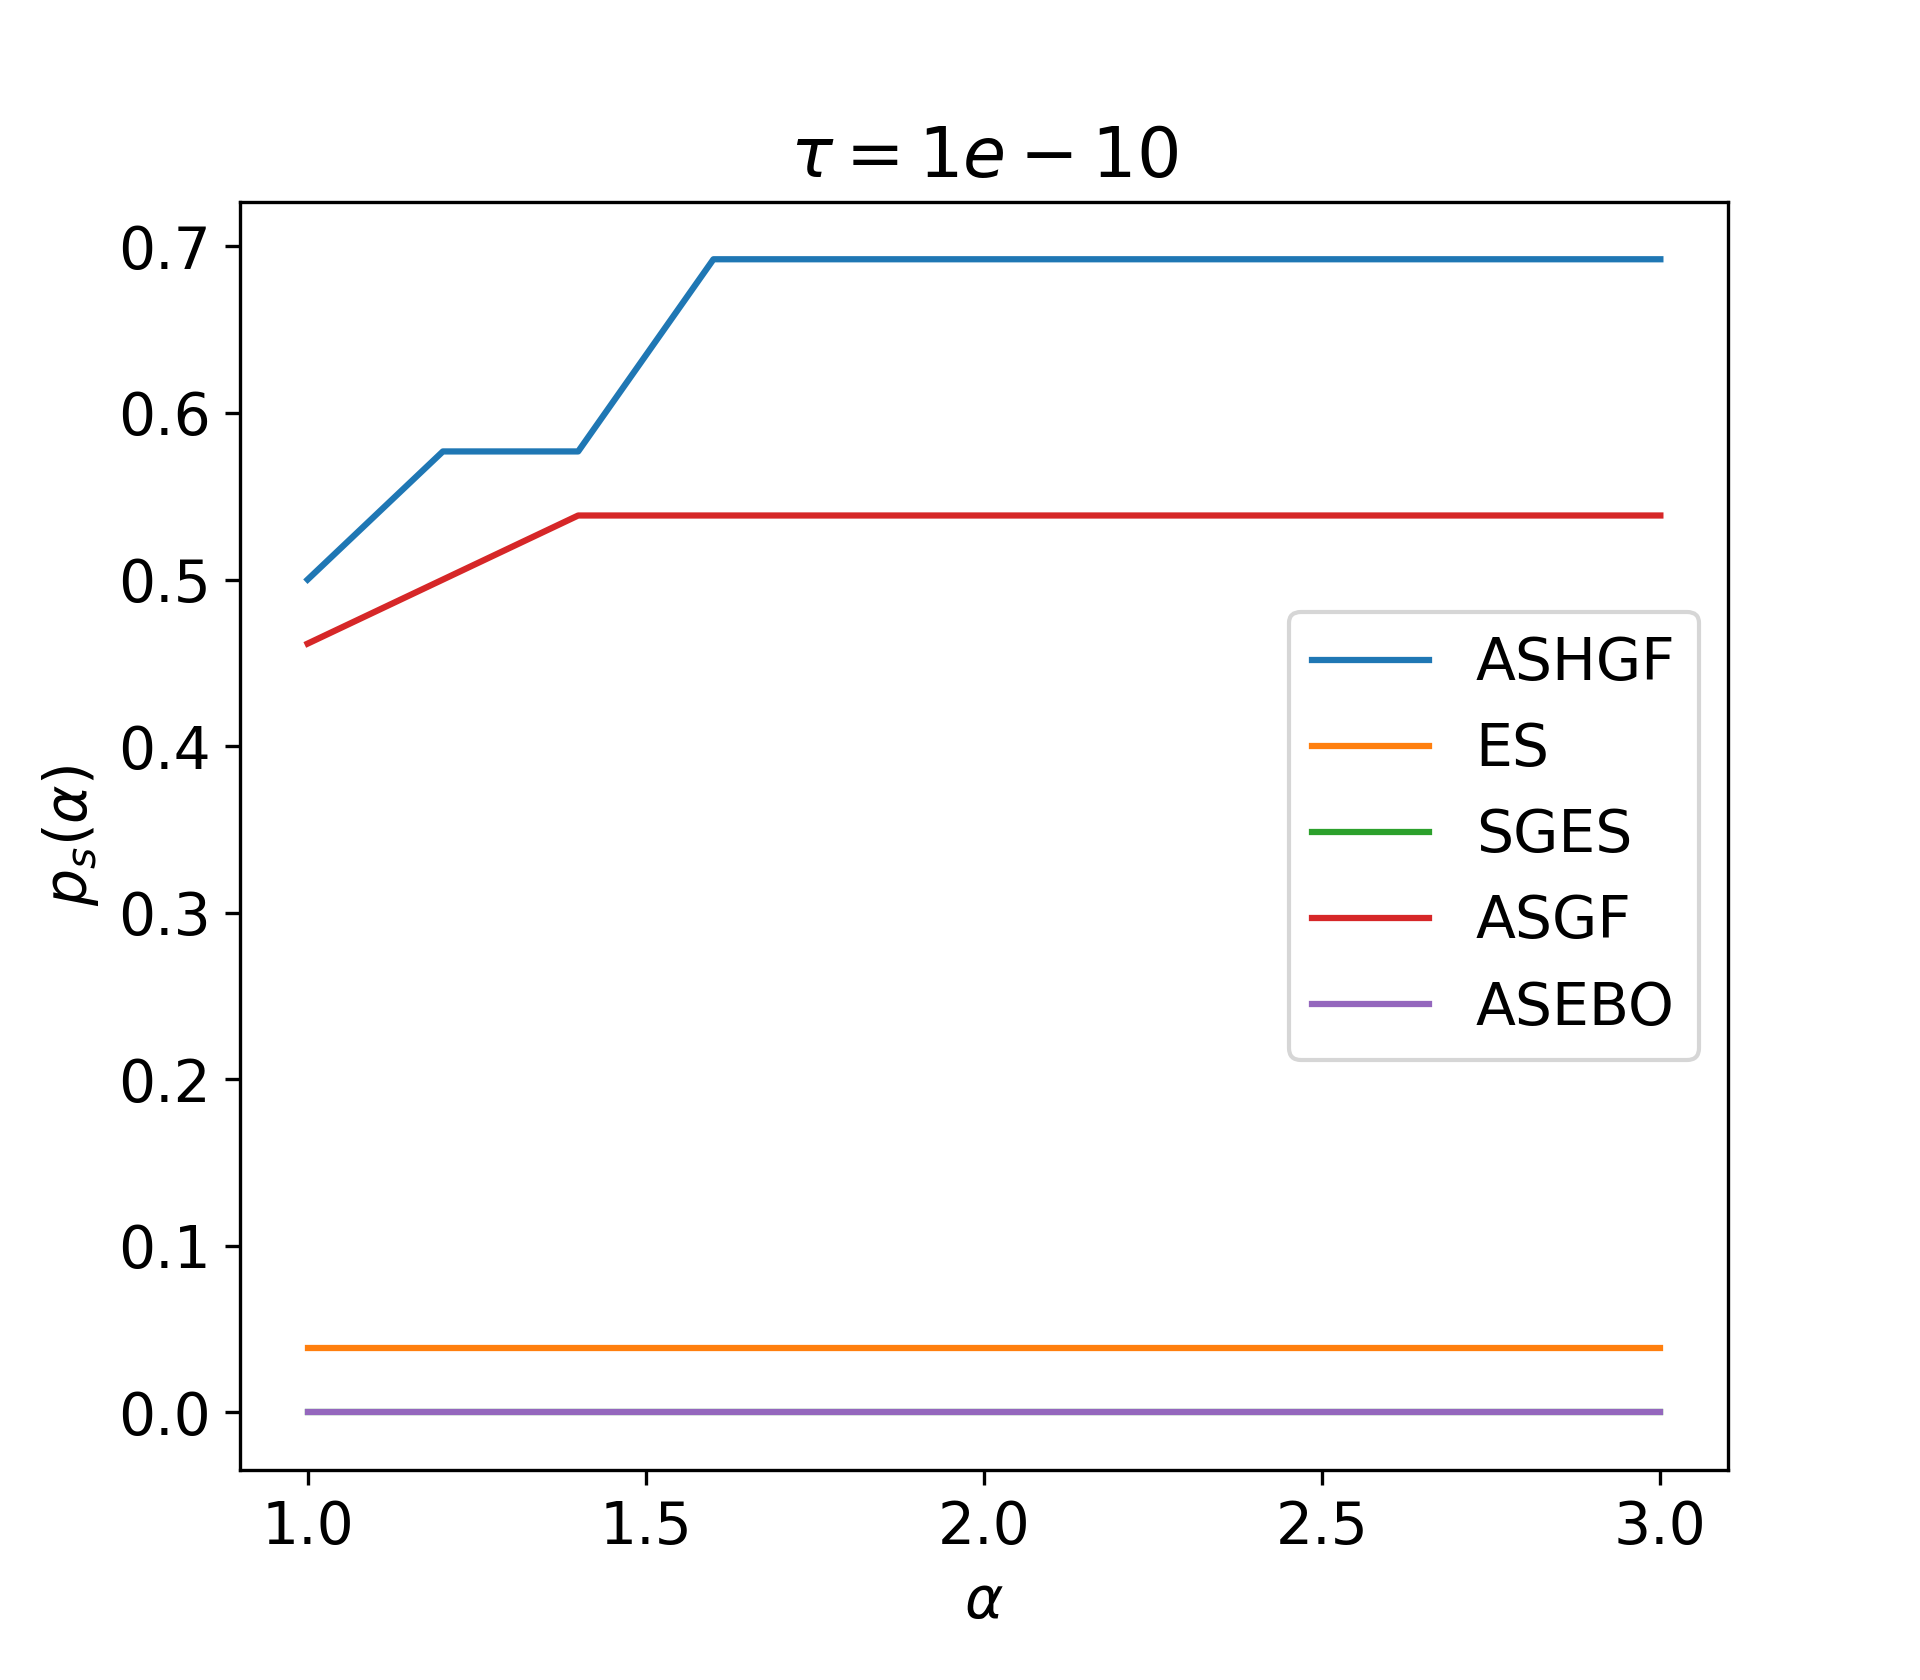
\includegraphics[width=1\textwidth]{figures/performance_profiles/100/performance_profile_100_10000000_1e-10.png}
\end{subfigure}
\caption{Performance profiles with $\mu_L = 10^{7}$}
\label{PerformanceProfiles100Mu10000000}
\end{figure}

\begin{figure}[H]
	\centering
	\begin{subfigure}{0.3\textwidth}
		\centering 
		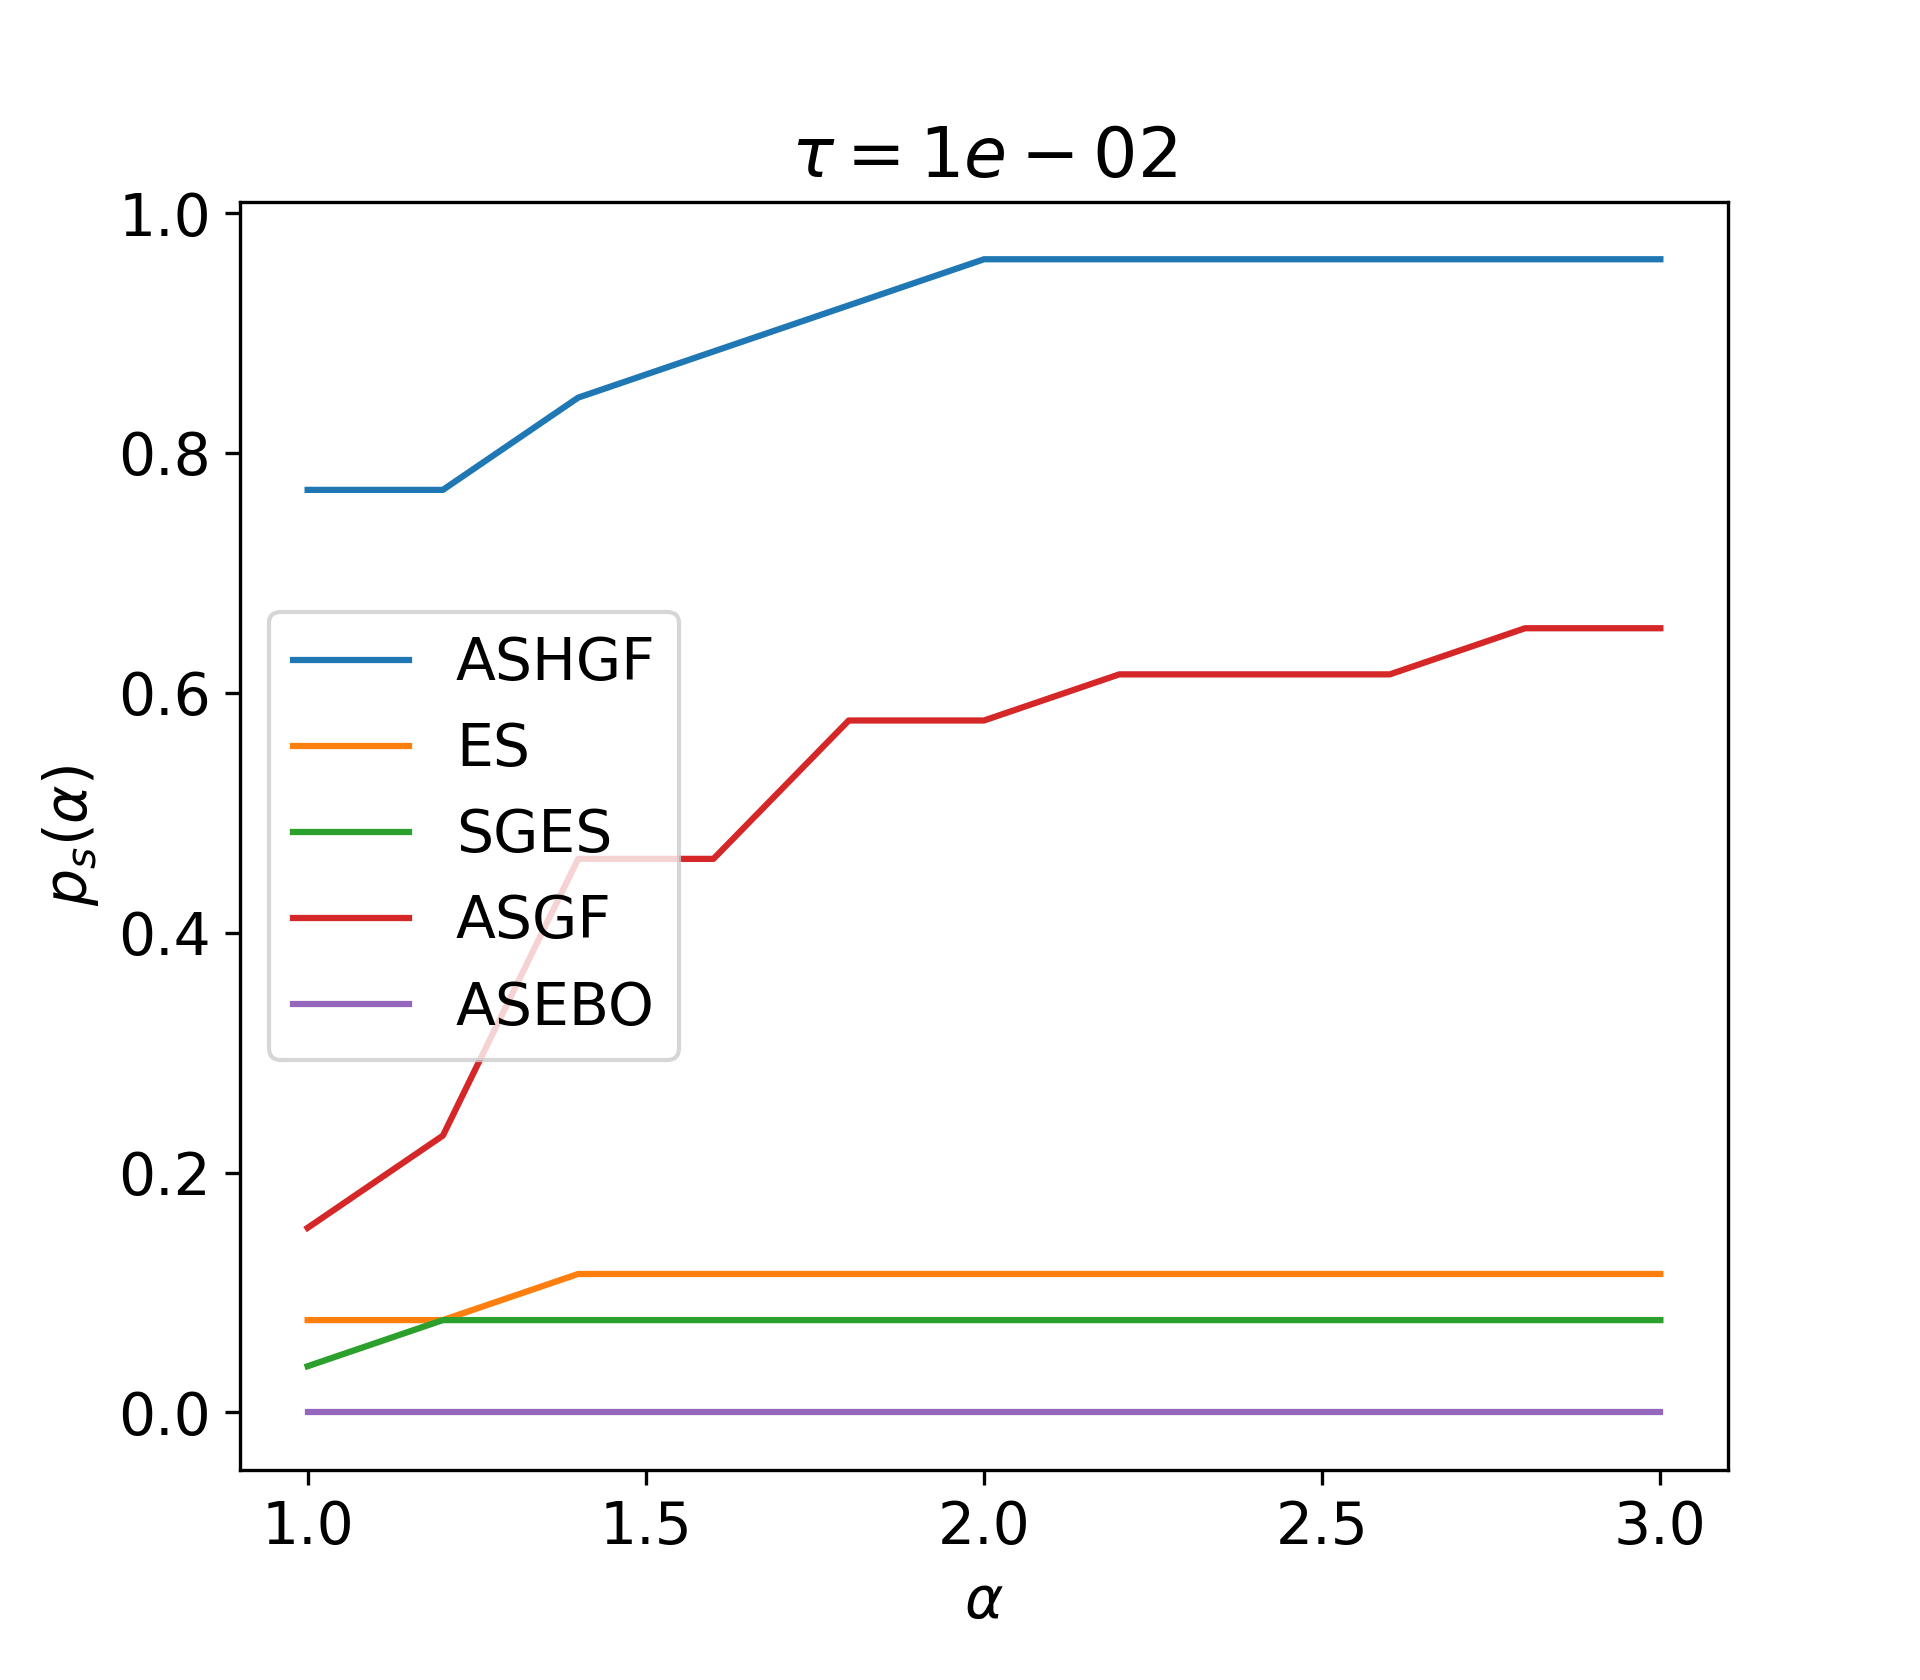
\includegraphics[width=1\textwidth]{figures/performance_profiles/100/performance_profile_100_100000000_1e-02.png}
	\end{subfigure}%
	\begin{subfigure}{0.3\textwidth}
		\centering 
		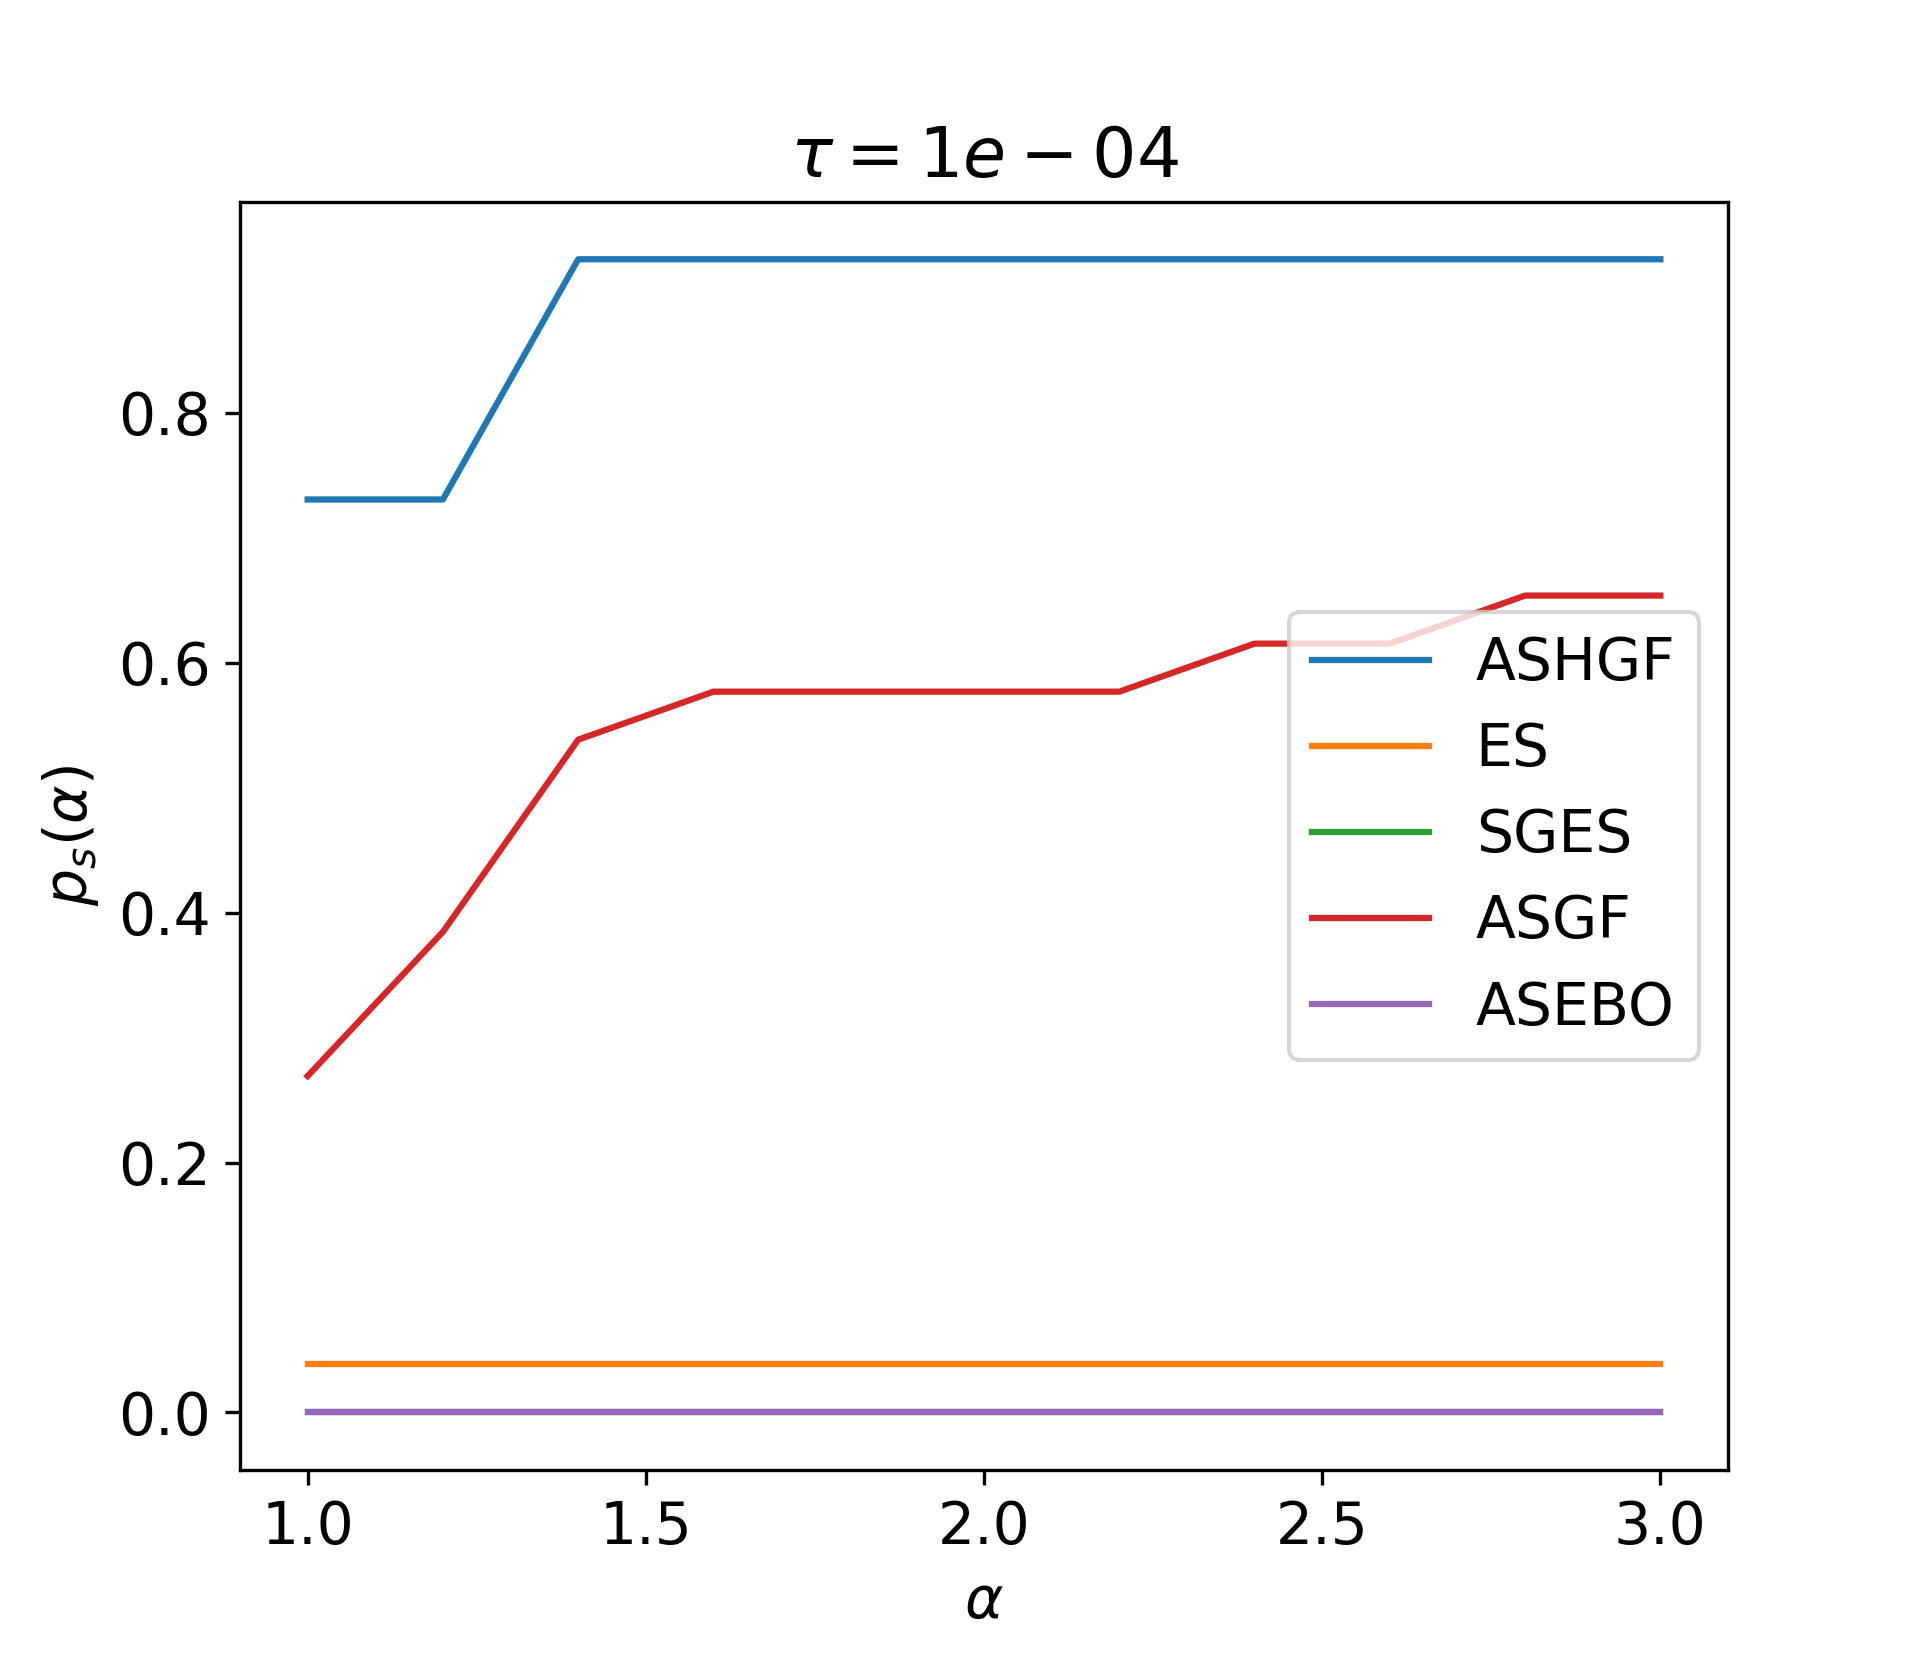
\includegraphics[width=1\textwidth]{figures/performance_profiles/100/performance_profile_100_100000000_1e-04.png}
	\end{subfigure}
	\begin{subfigure}{0.3\textwidth}
		\centering 
		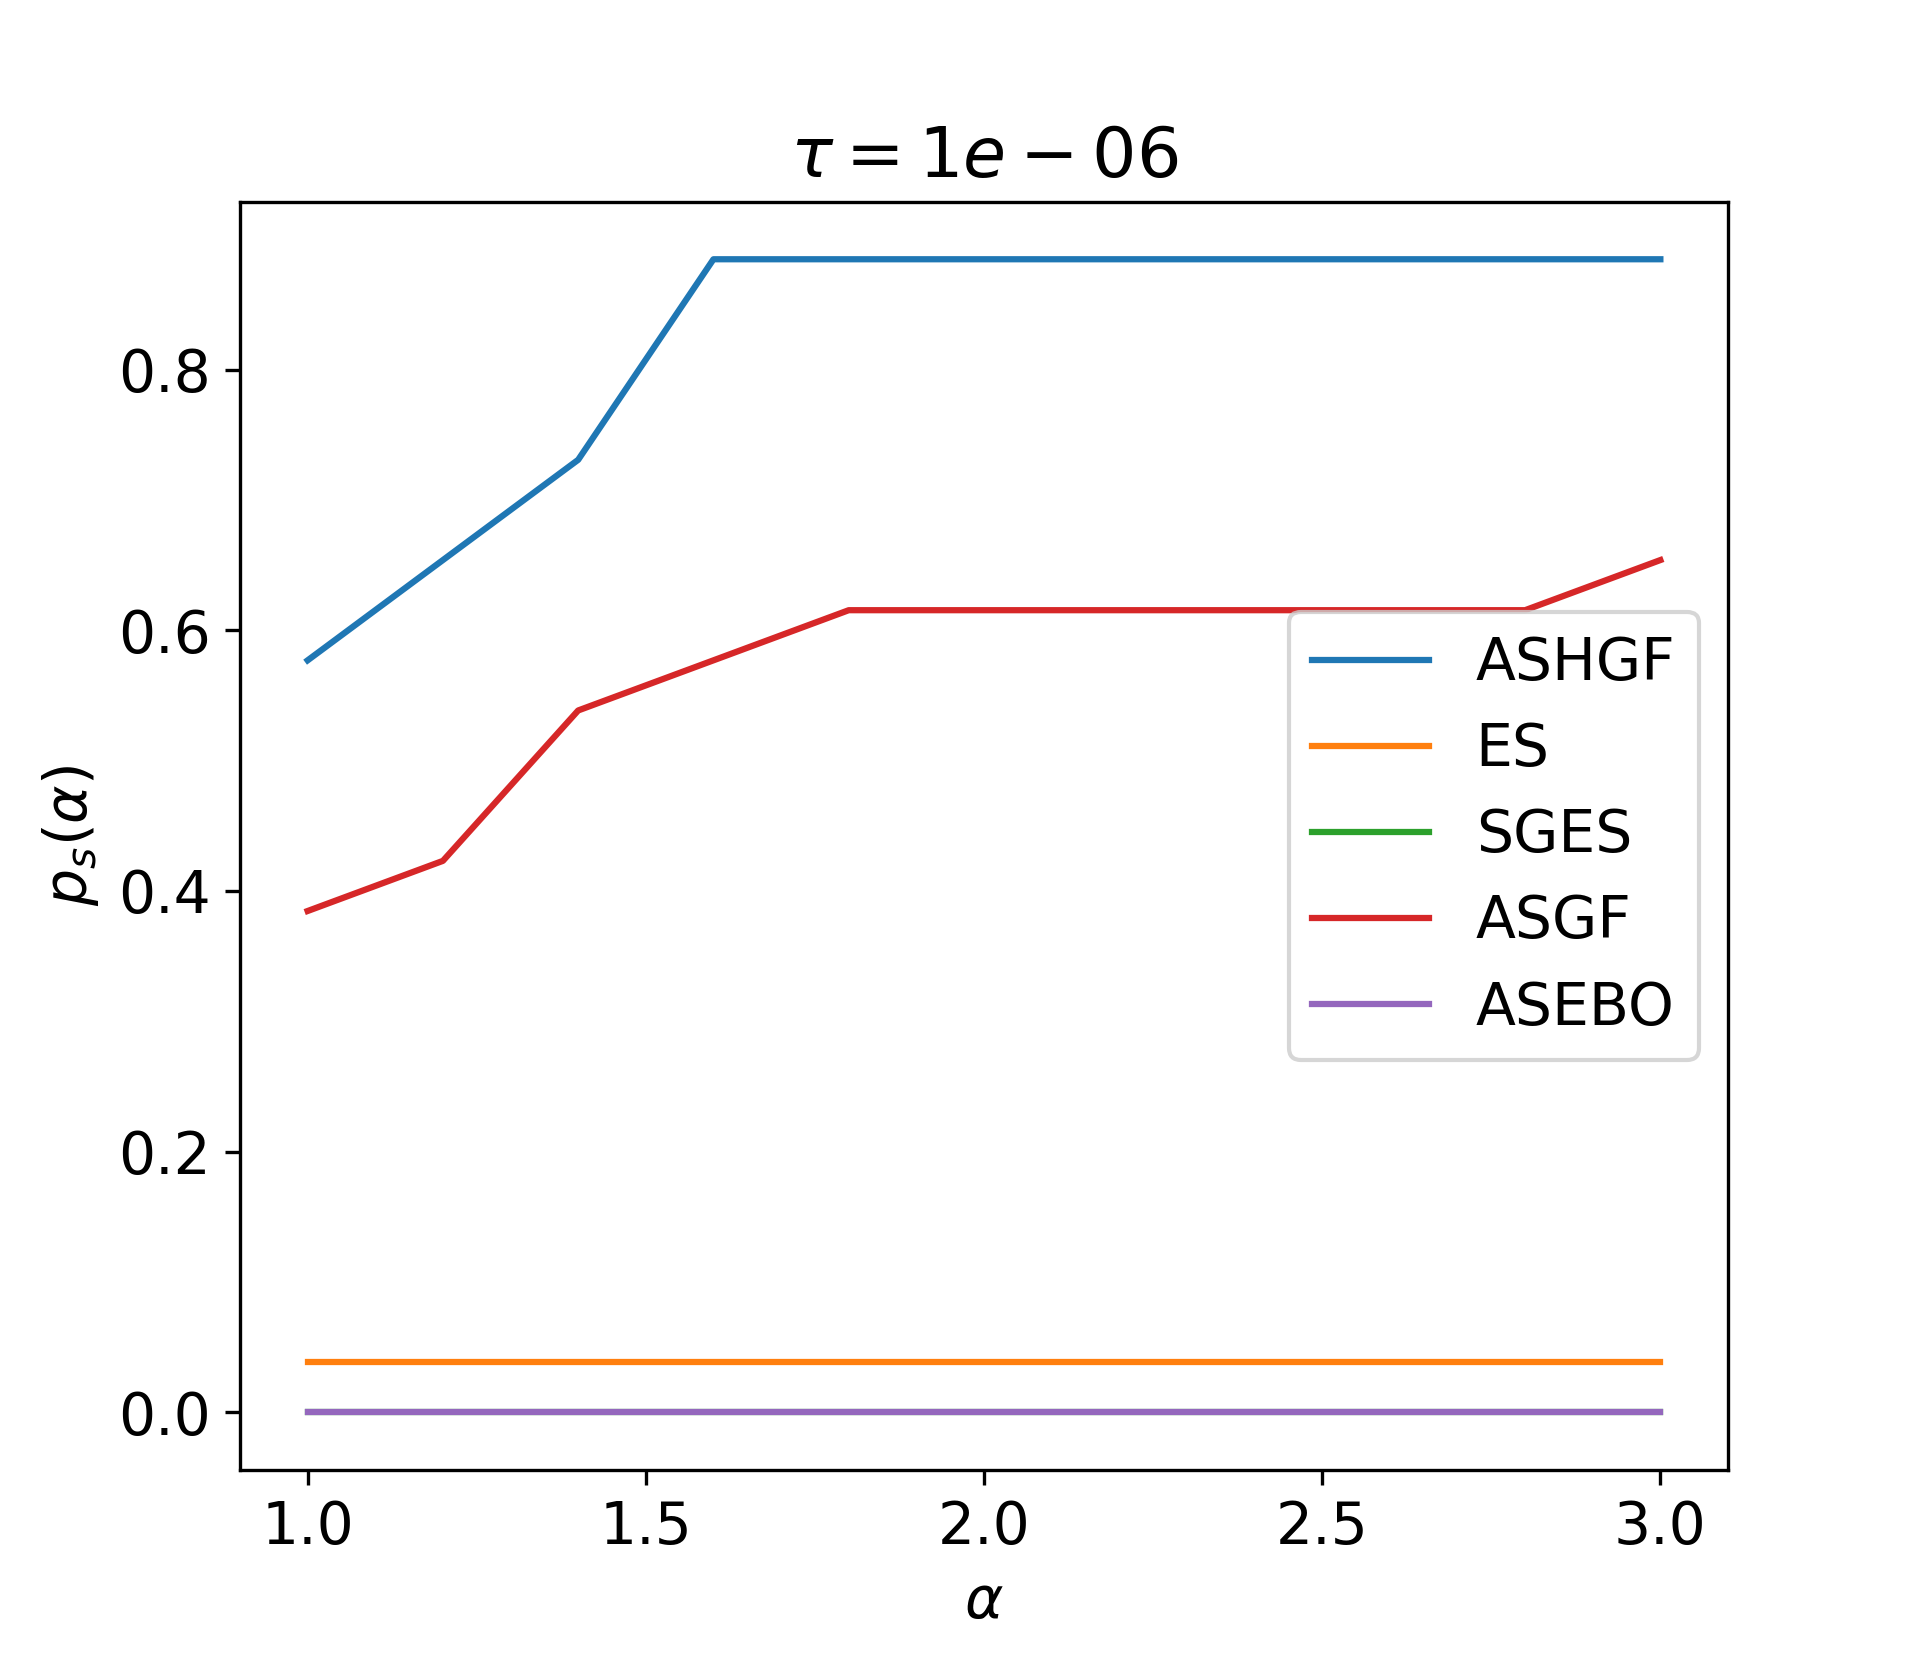
\includegraphics[width=1\textwidth]{figures/performance_profiles/100/performance_profile_100_100000000_1e-06.png}
	\end{subfigure}
	\centering
	\begin{subfigure}{0.3\textwidth}
		\centering 
		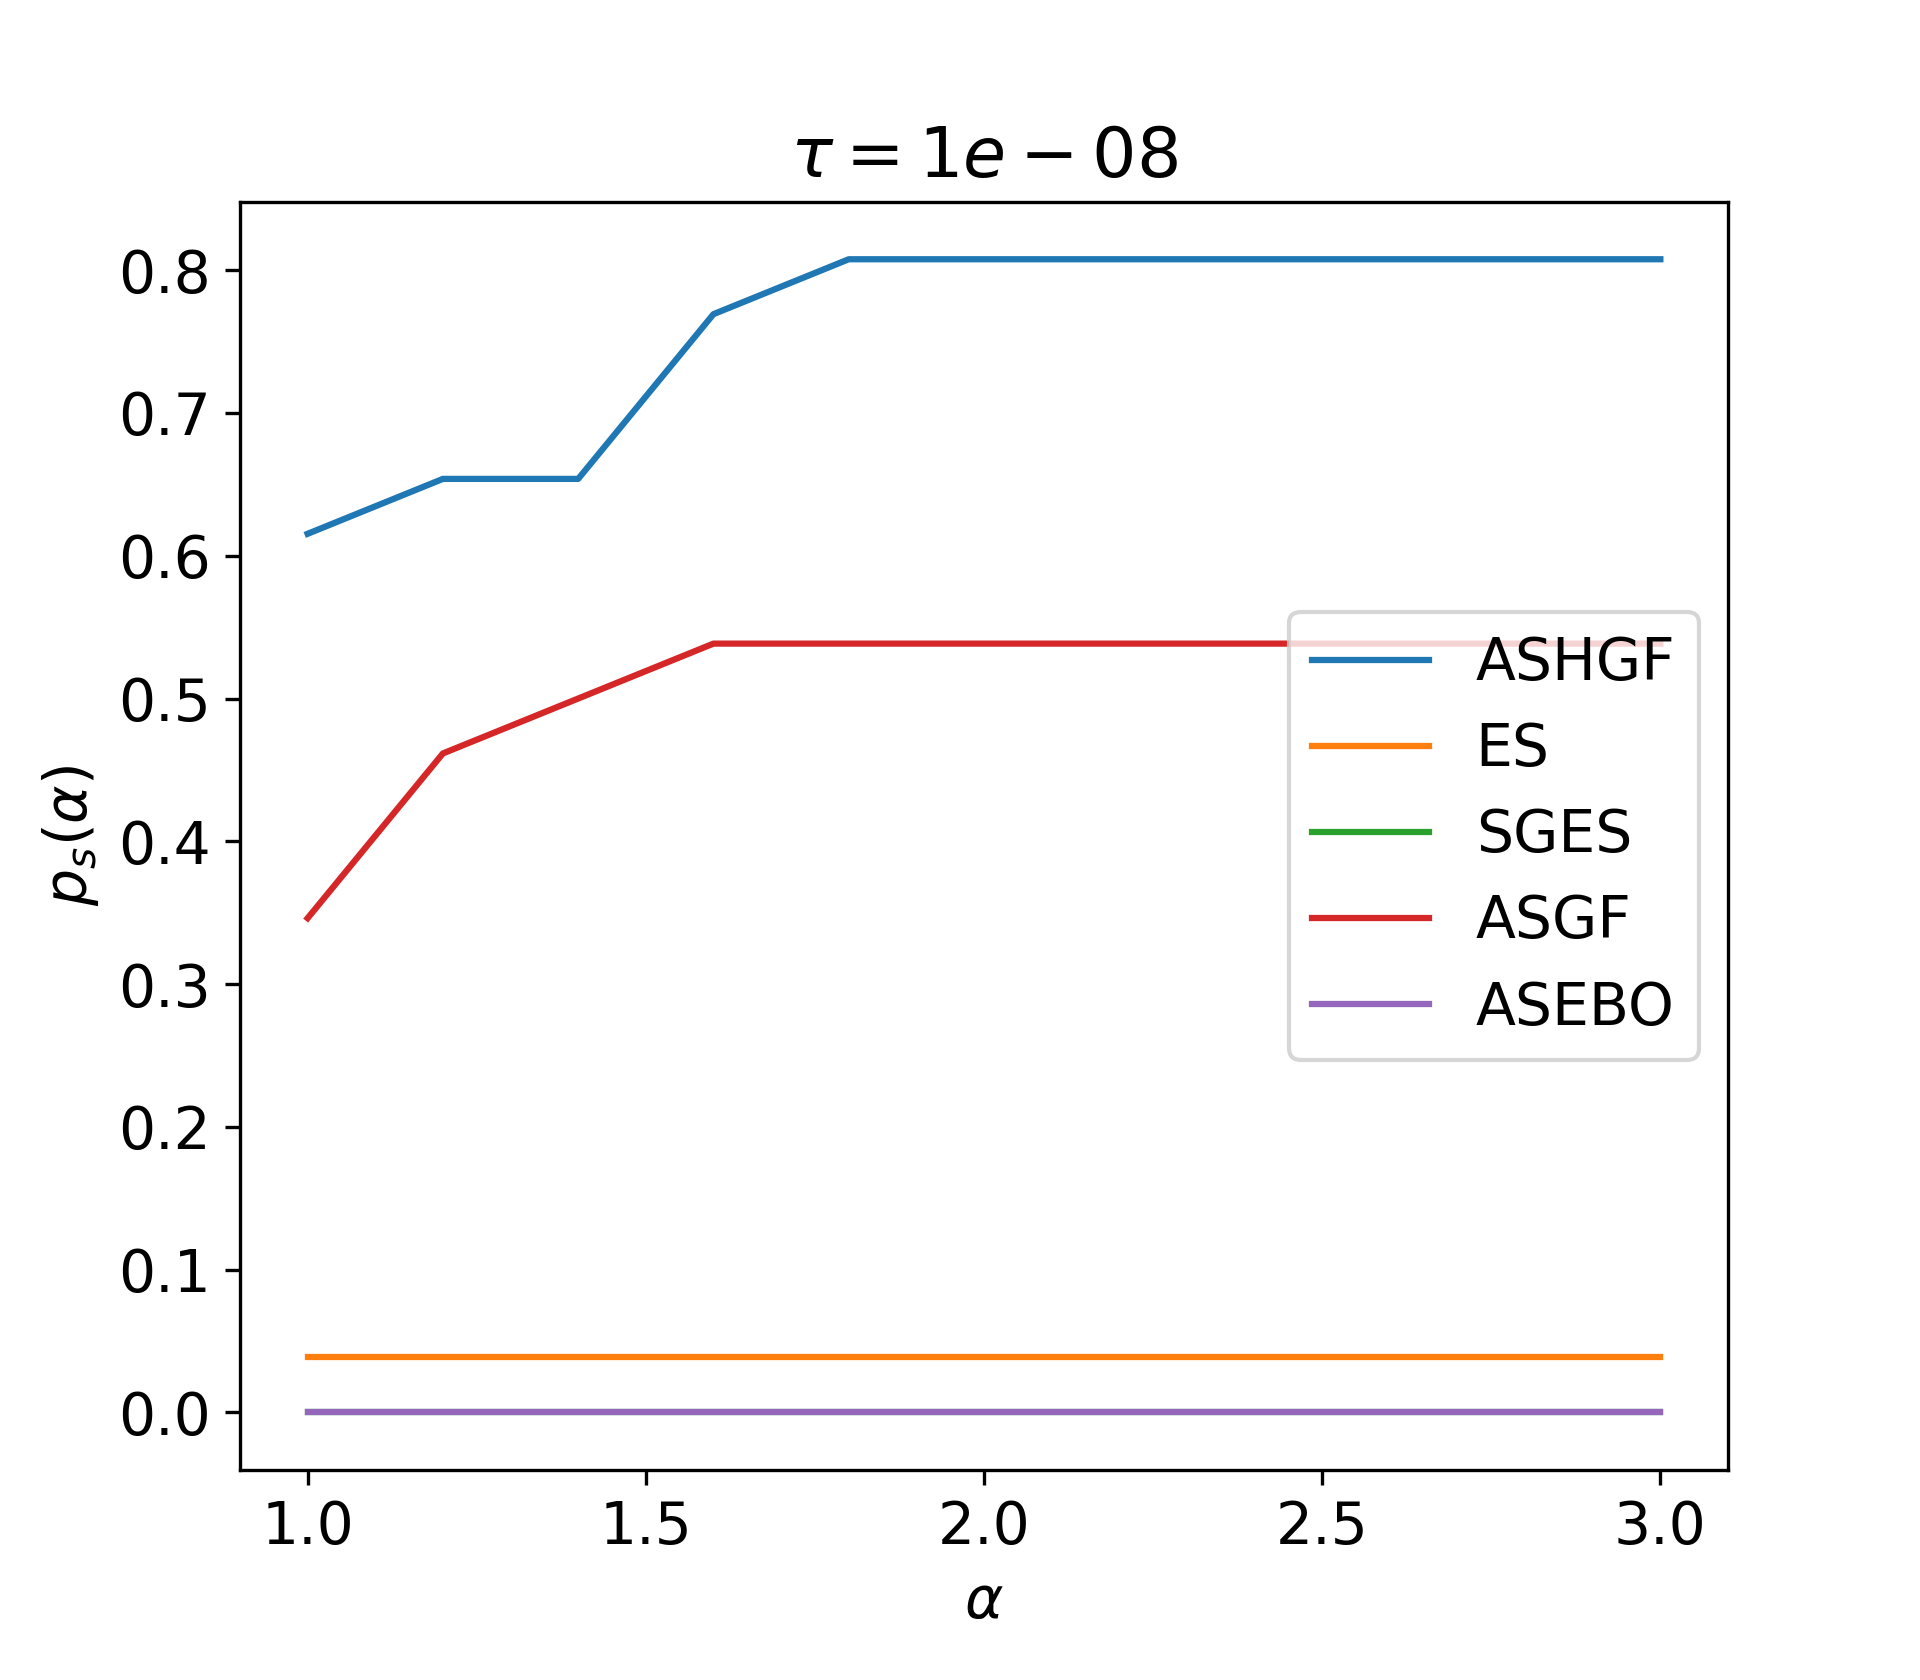
\includegraphics[width=1\textwidth]{figures/performance_profiles/100/performance_profile_100_100000000_1e-08.png}
	\end{subfigure}%
	\begin{subfigure}{0.3\textwidth}
		\centering 
		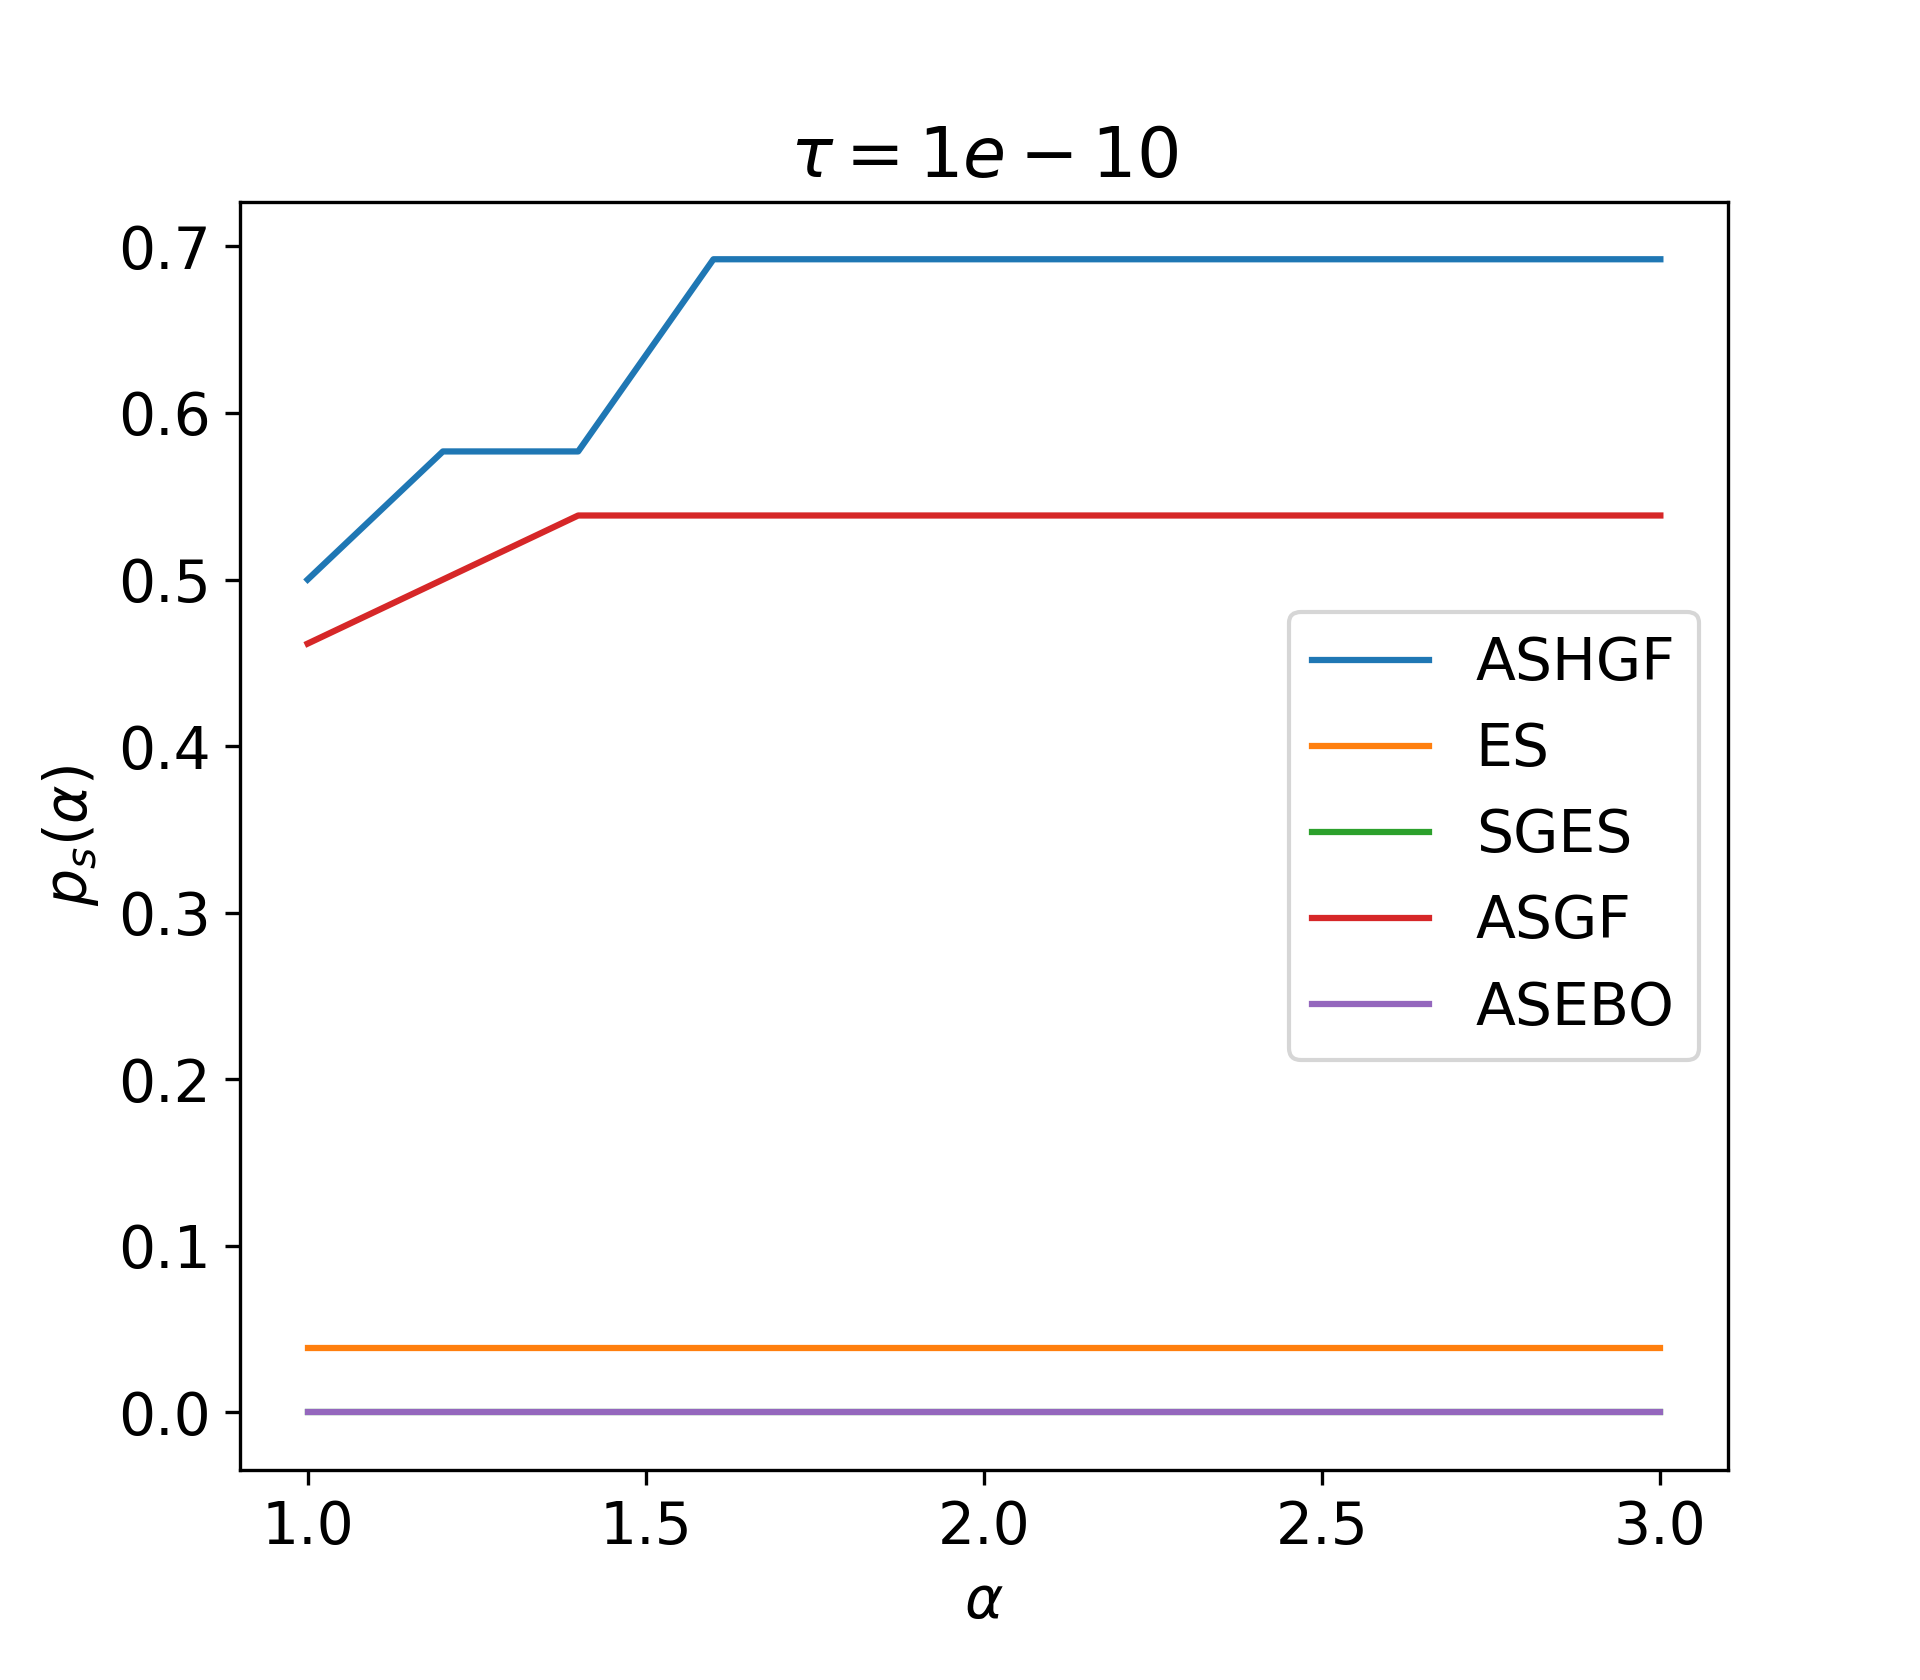
\includegraphics[width=1\textwidth]{figures/performance_profiles/100/performance_profile_100_100000000_1e-10.png}
	\end{subfigure}
	\caption{Performance profiles with $\mu_L = 10^{8}$}
	\label{PerformanceProfiles100Mu100000000}
\end{figure}

\subsubsection{Dimension 1000}

\begin{figure}[H]
\centering
\begin{subfigure}{0.3\textwidth}
  \centering 
  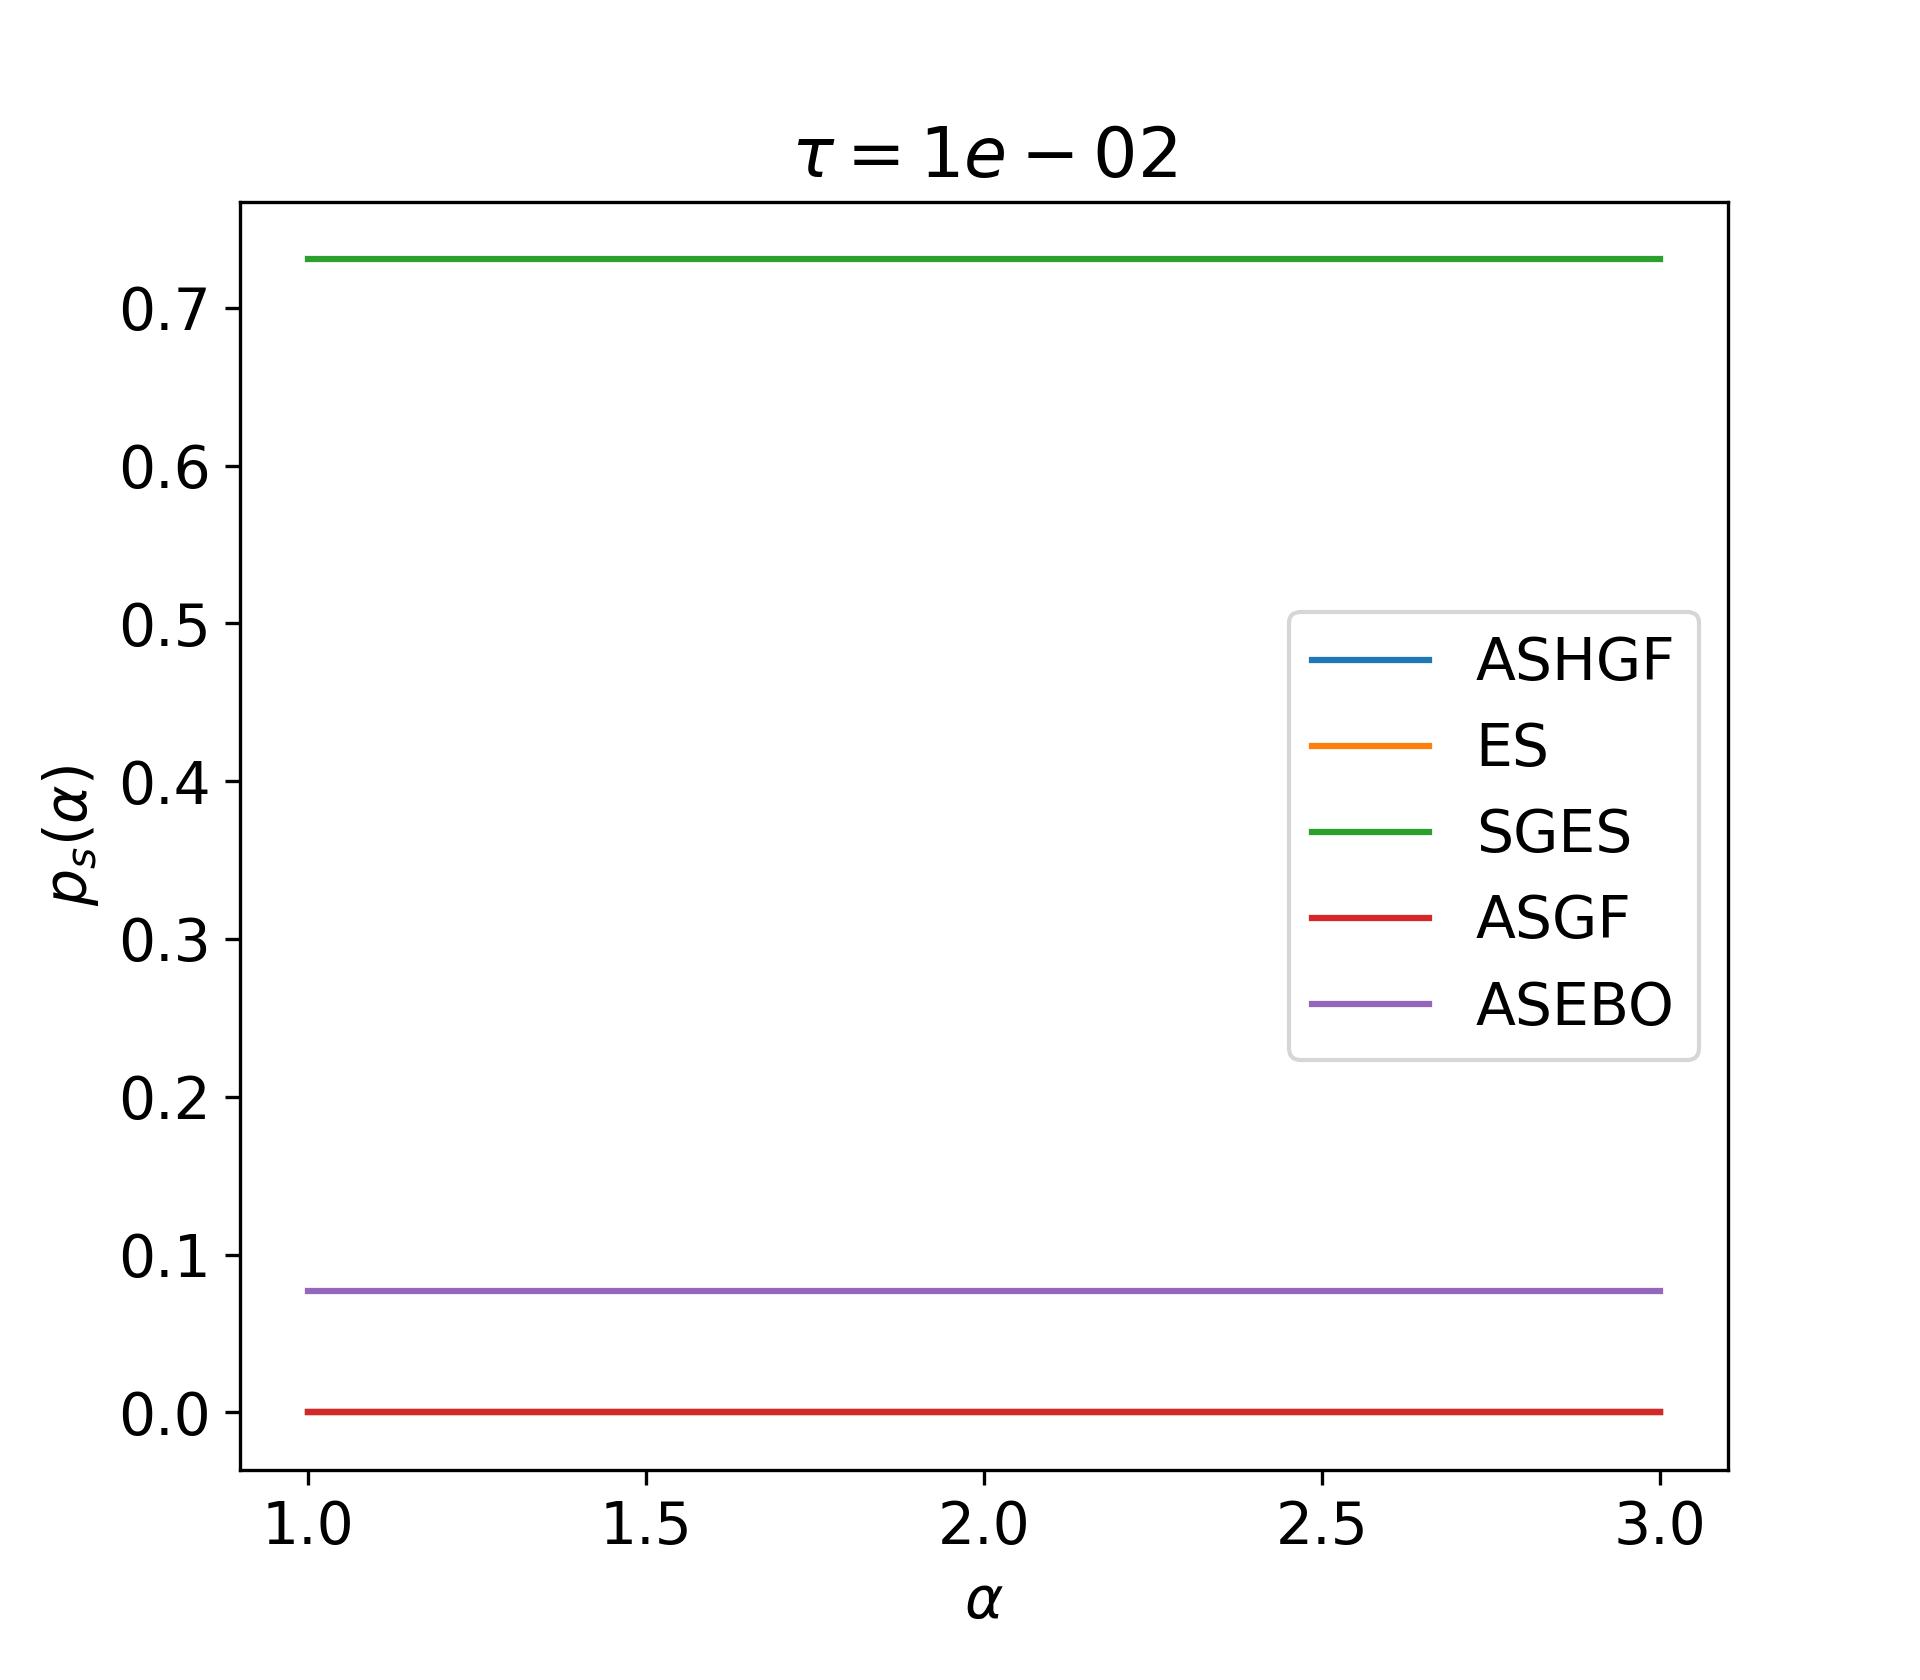
\includegraphics[width=1\textwidth]{figures/performance_profiles/1000/performance_profile_1000_10000_1e-02.png}
\end{subfigure}%
\begin{subfigure}{0.3\textwidth}
  \centering 
  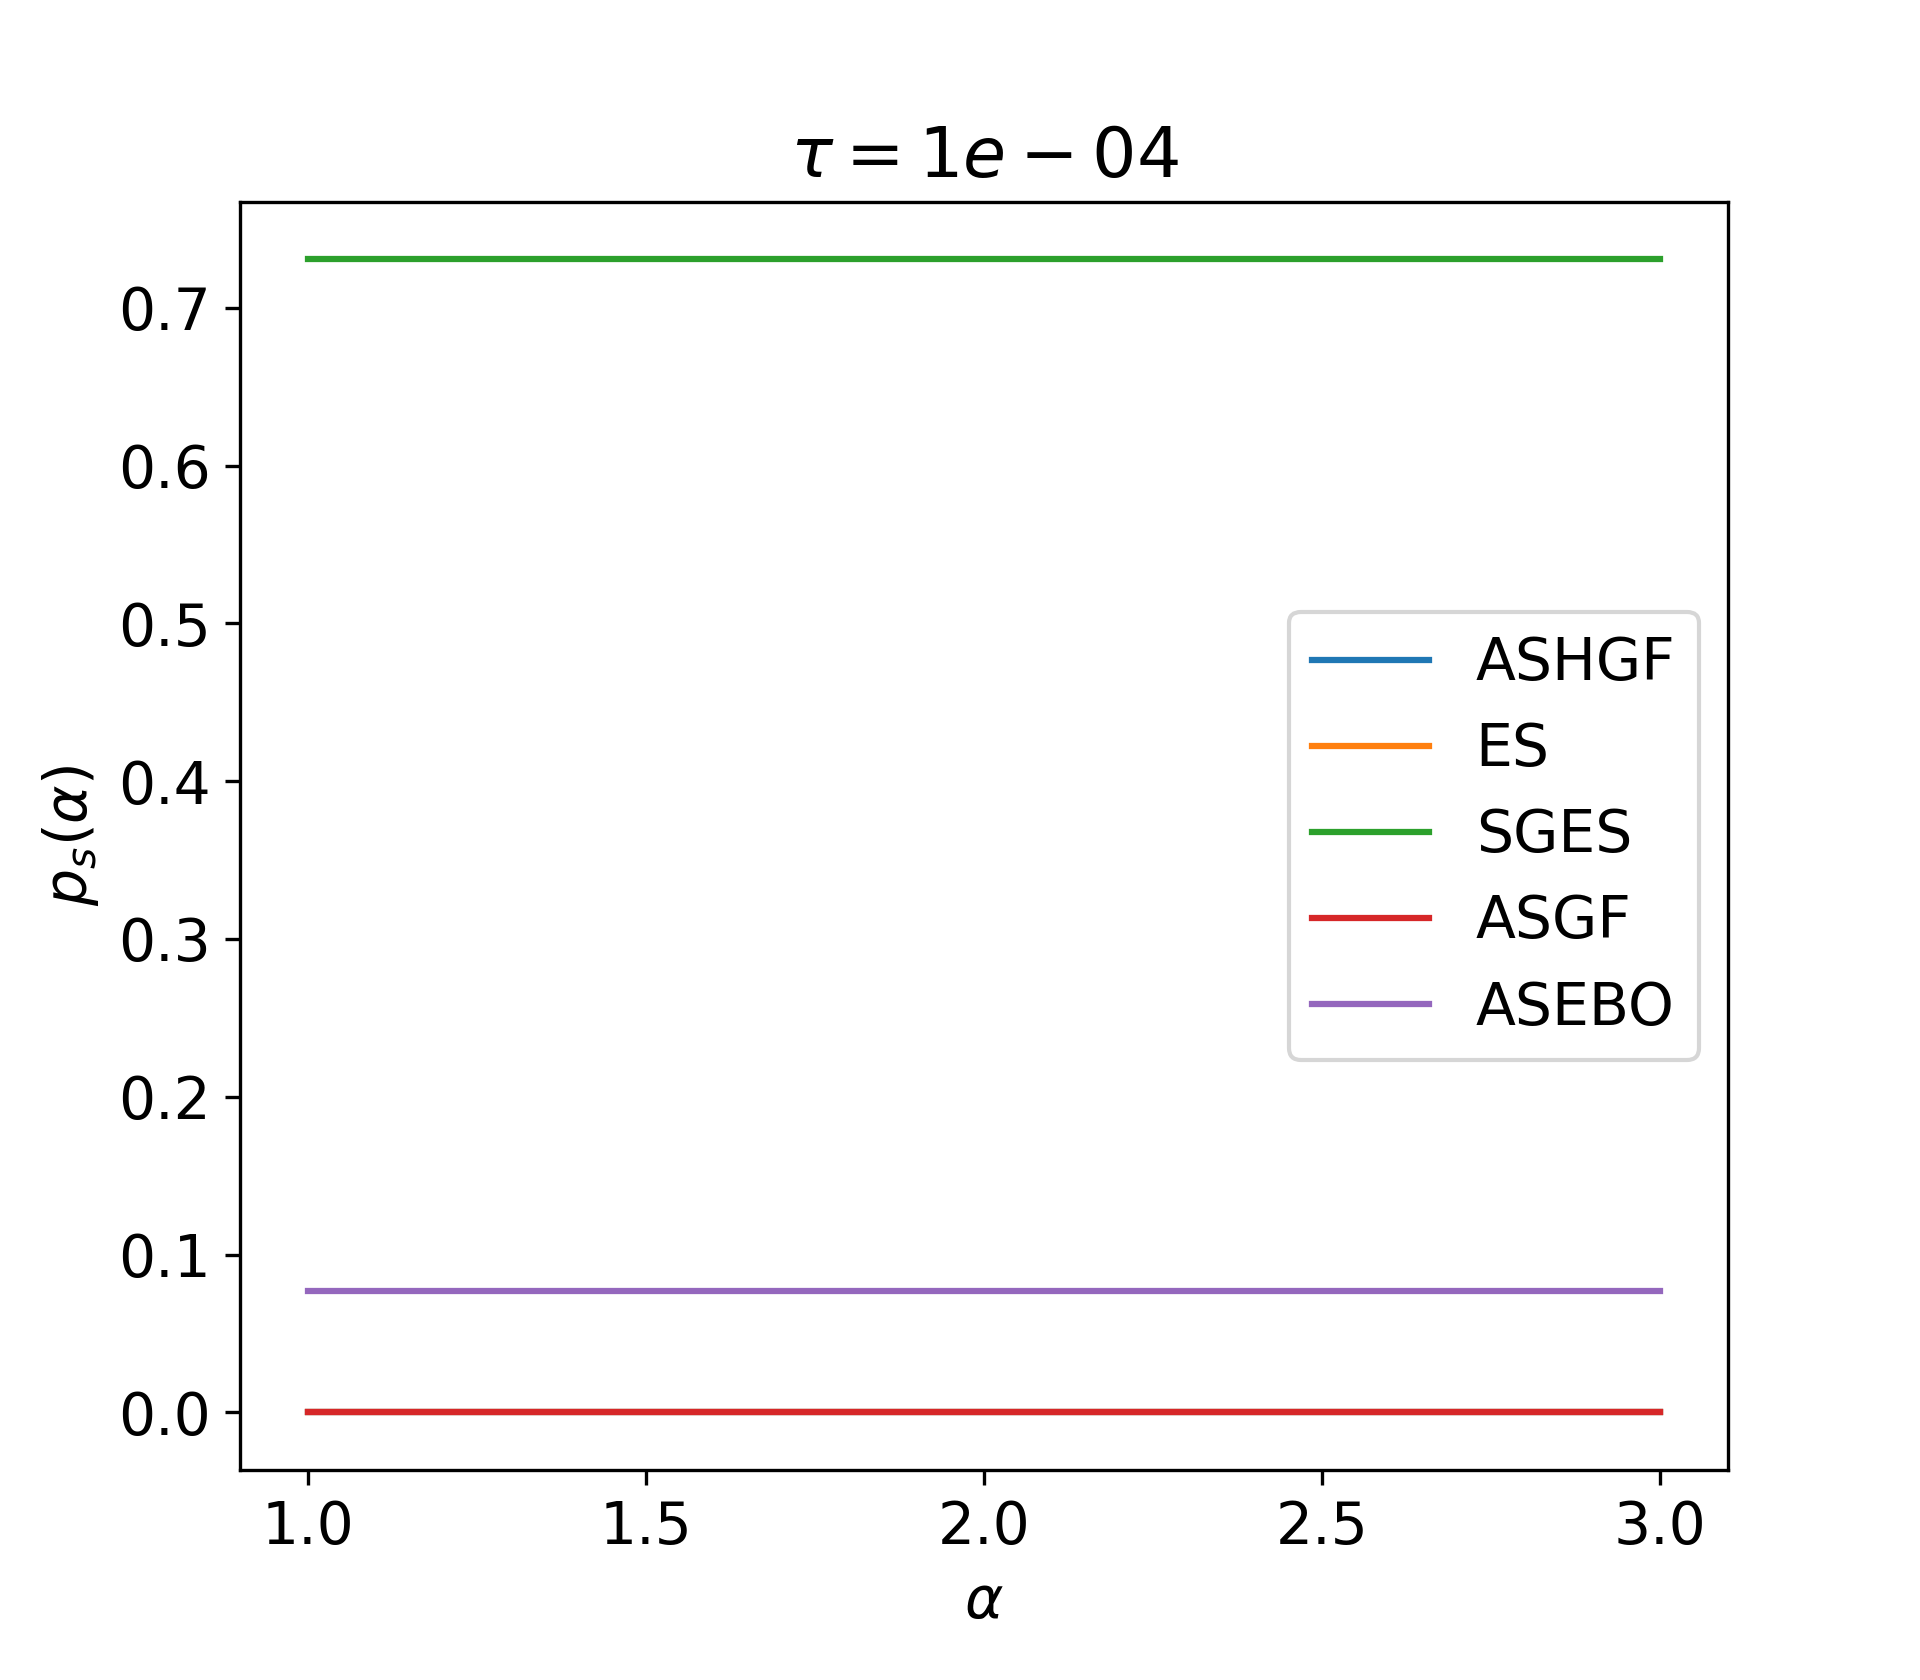
\includegraphics[width=1\textwidth]{figures/performance_profiles/1000/performance_profile_1000_10000_1e-04.png}
\end{subfigure}
\begin{subfigure}{0.3\textwidth}
  \centering 
  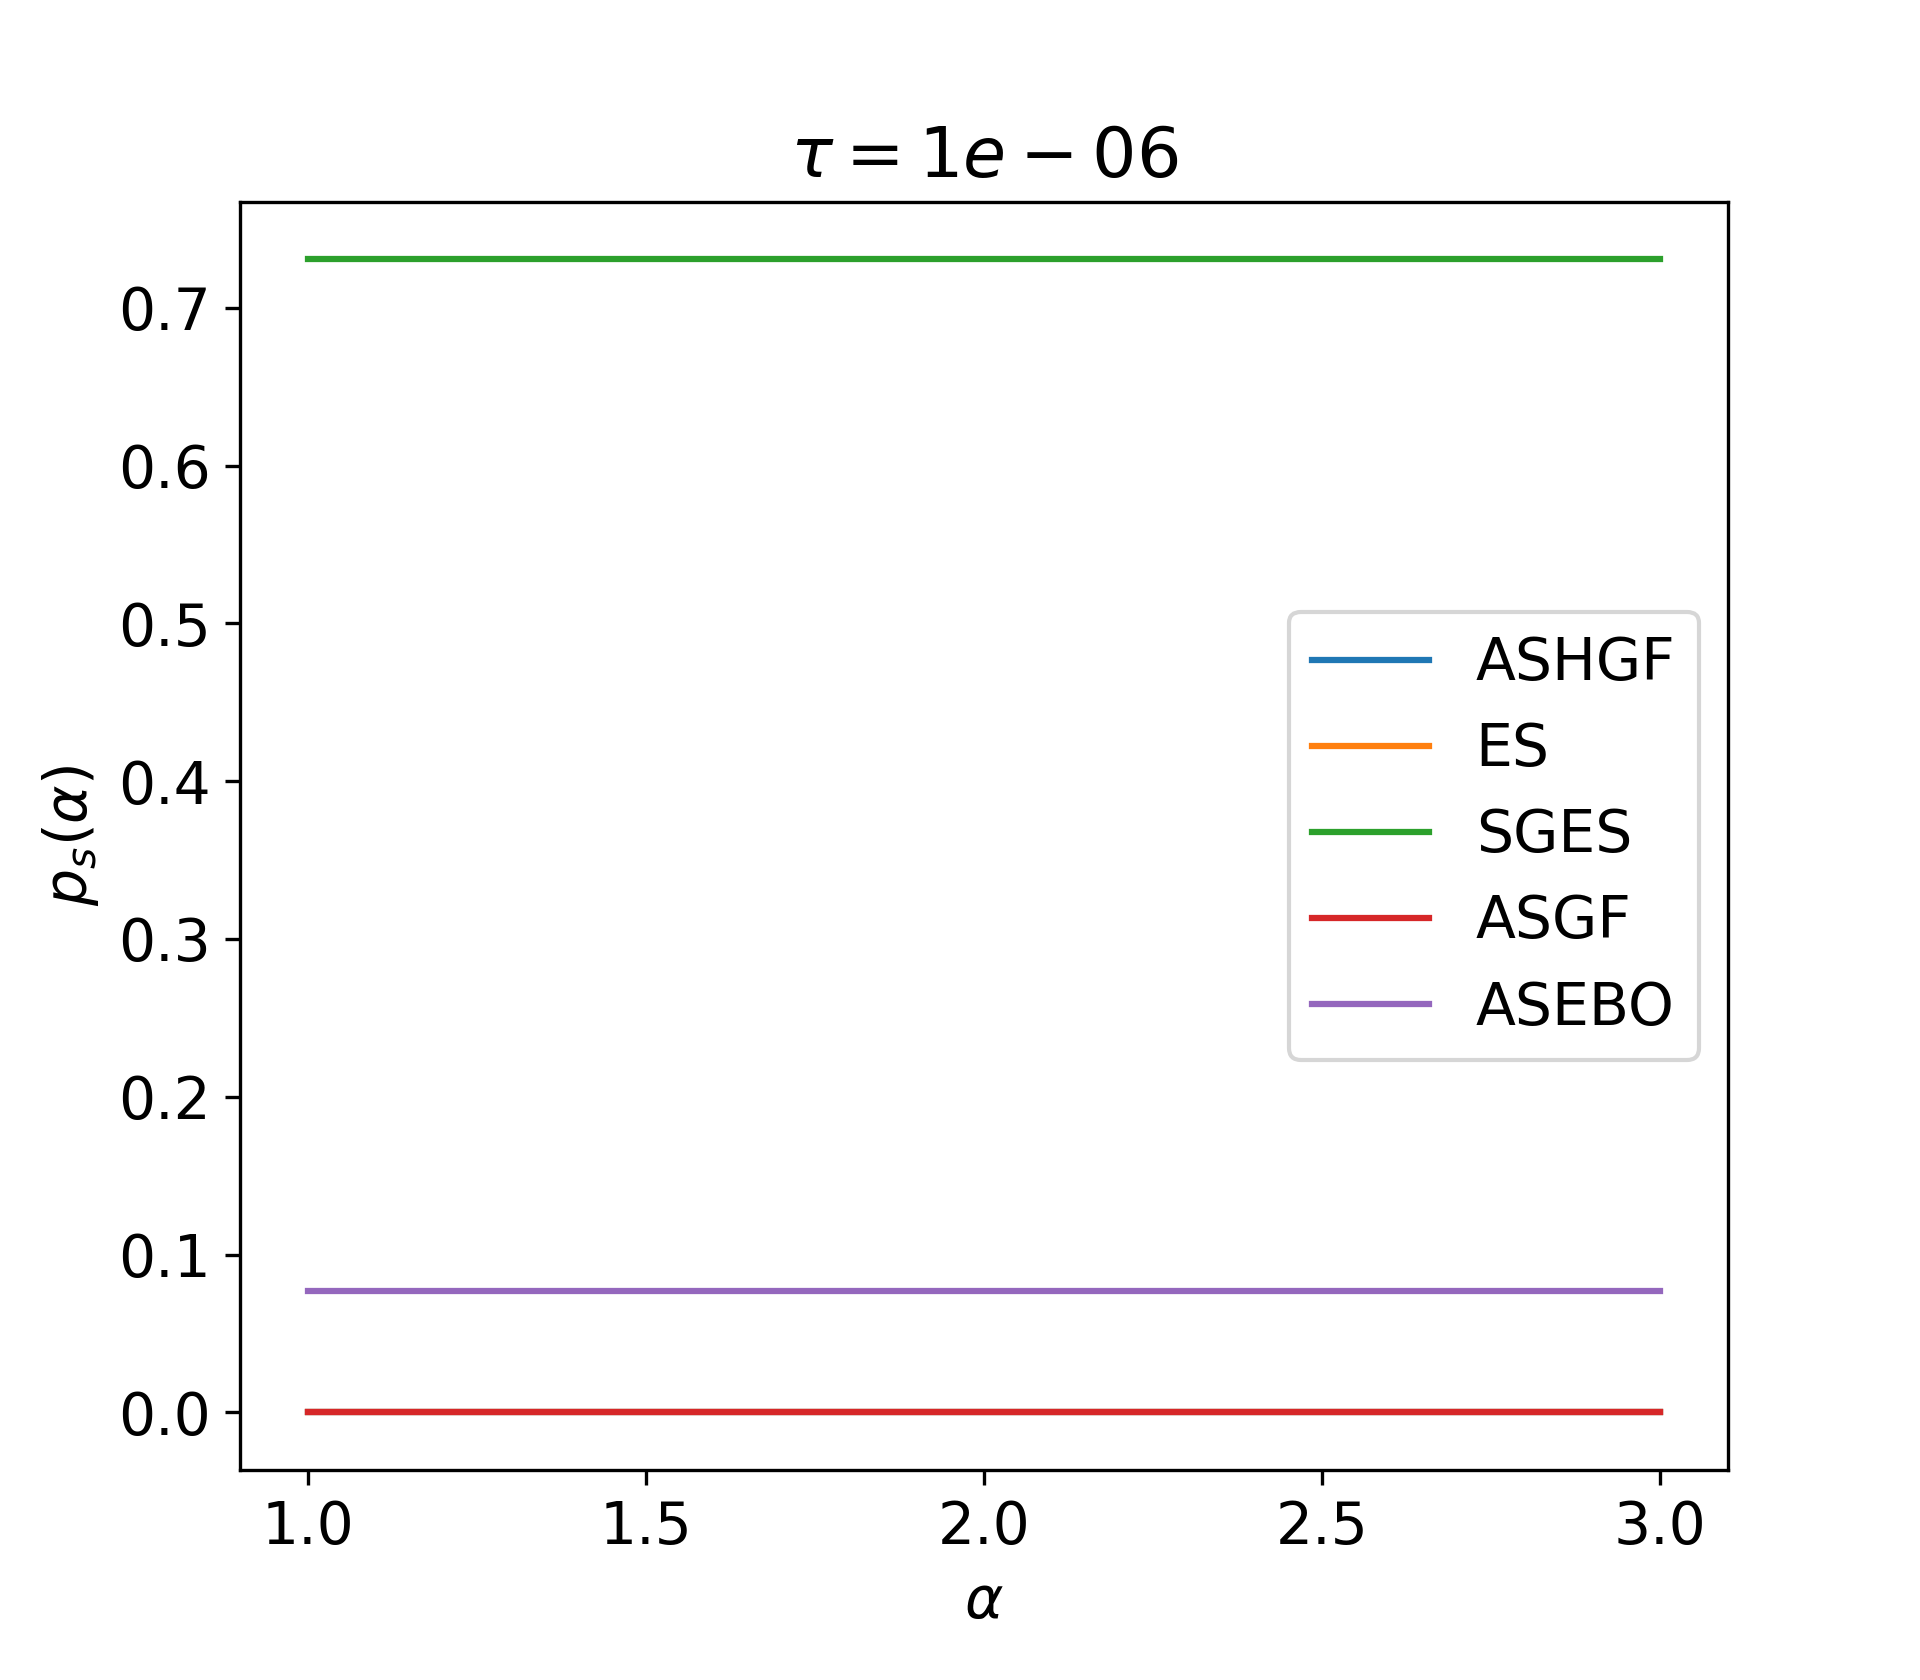
\includegraphics[width=1\textwidth]{figures/performance_profiles/1000/performance_profile_1000_10000_1e-06.png}
\end{subfigure}
\centering
\begin{subfigure}{0.3\textwidth}
  \centering 
  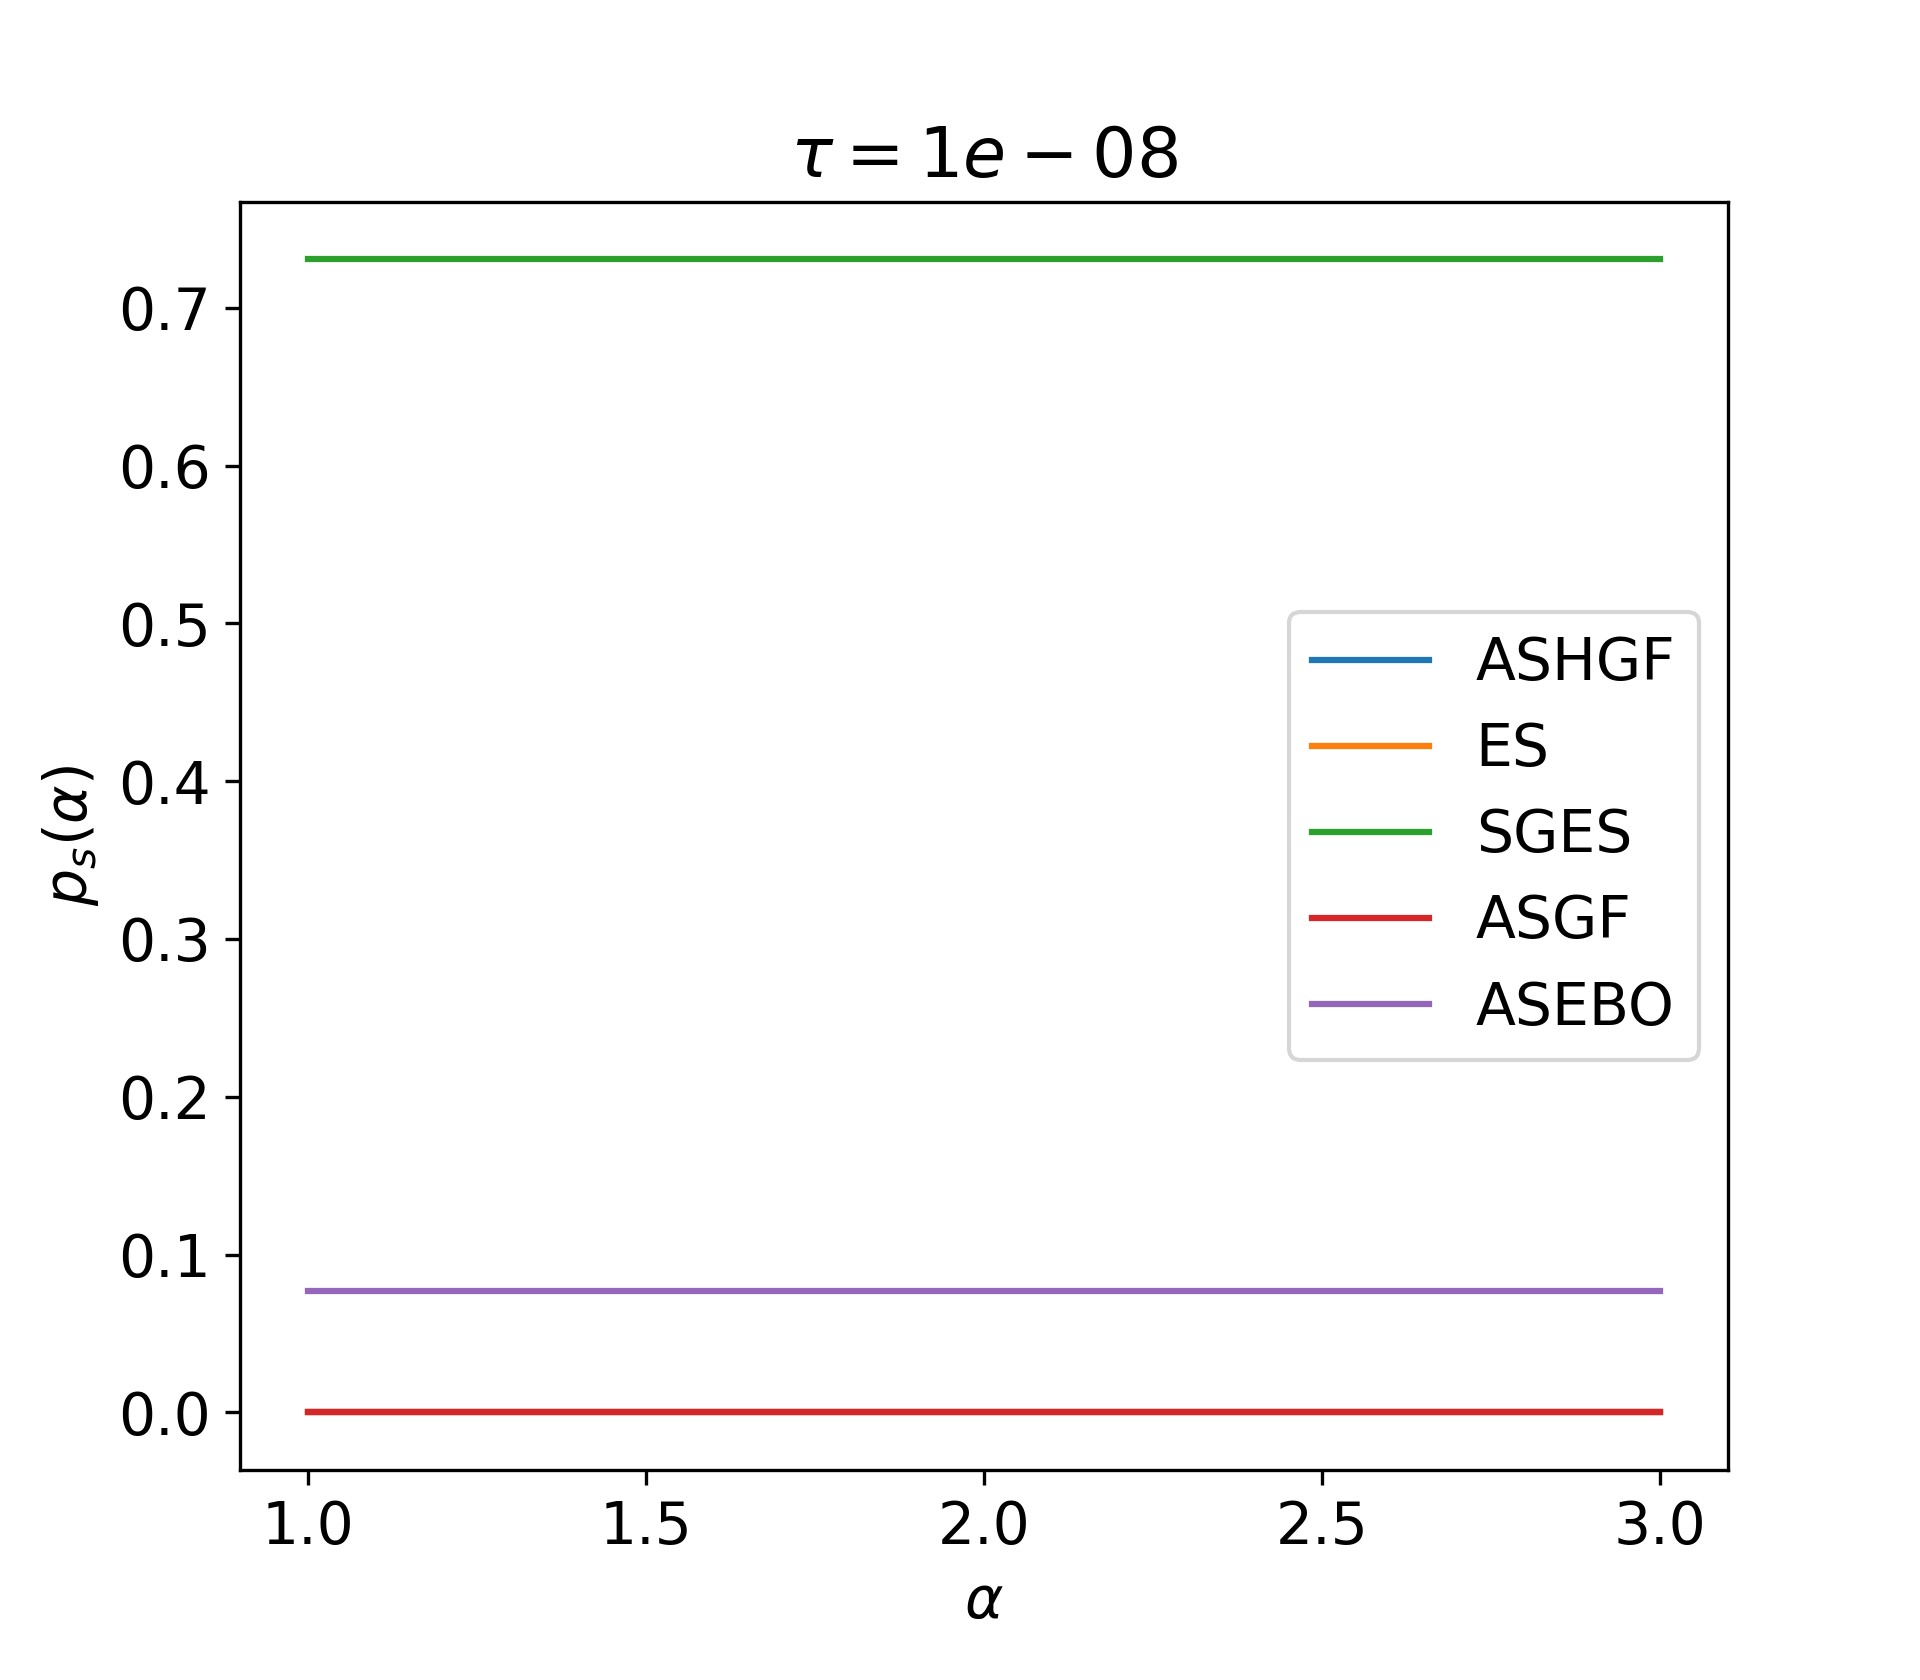
\includegraphics[width=1\textwidth]{figures/performance_profiles/1000/performance_profile_1000_10000_1e-08.png}
\end{subfigure}%
\begin{subfigure}{0.3\textwidth}
  \centering 
  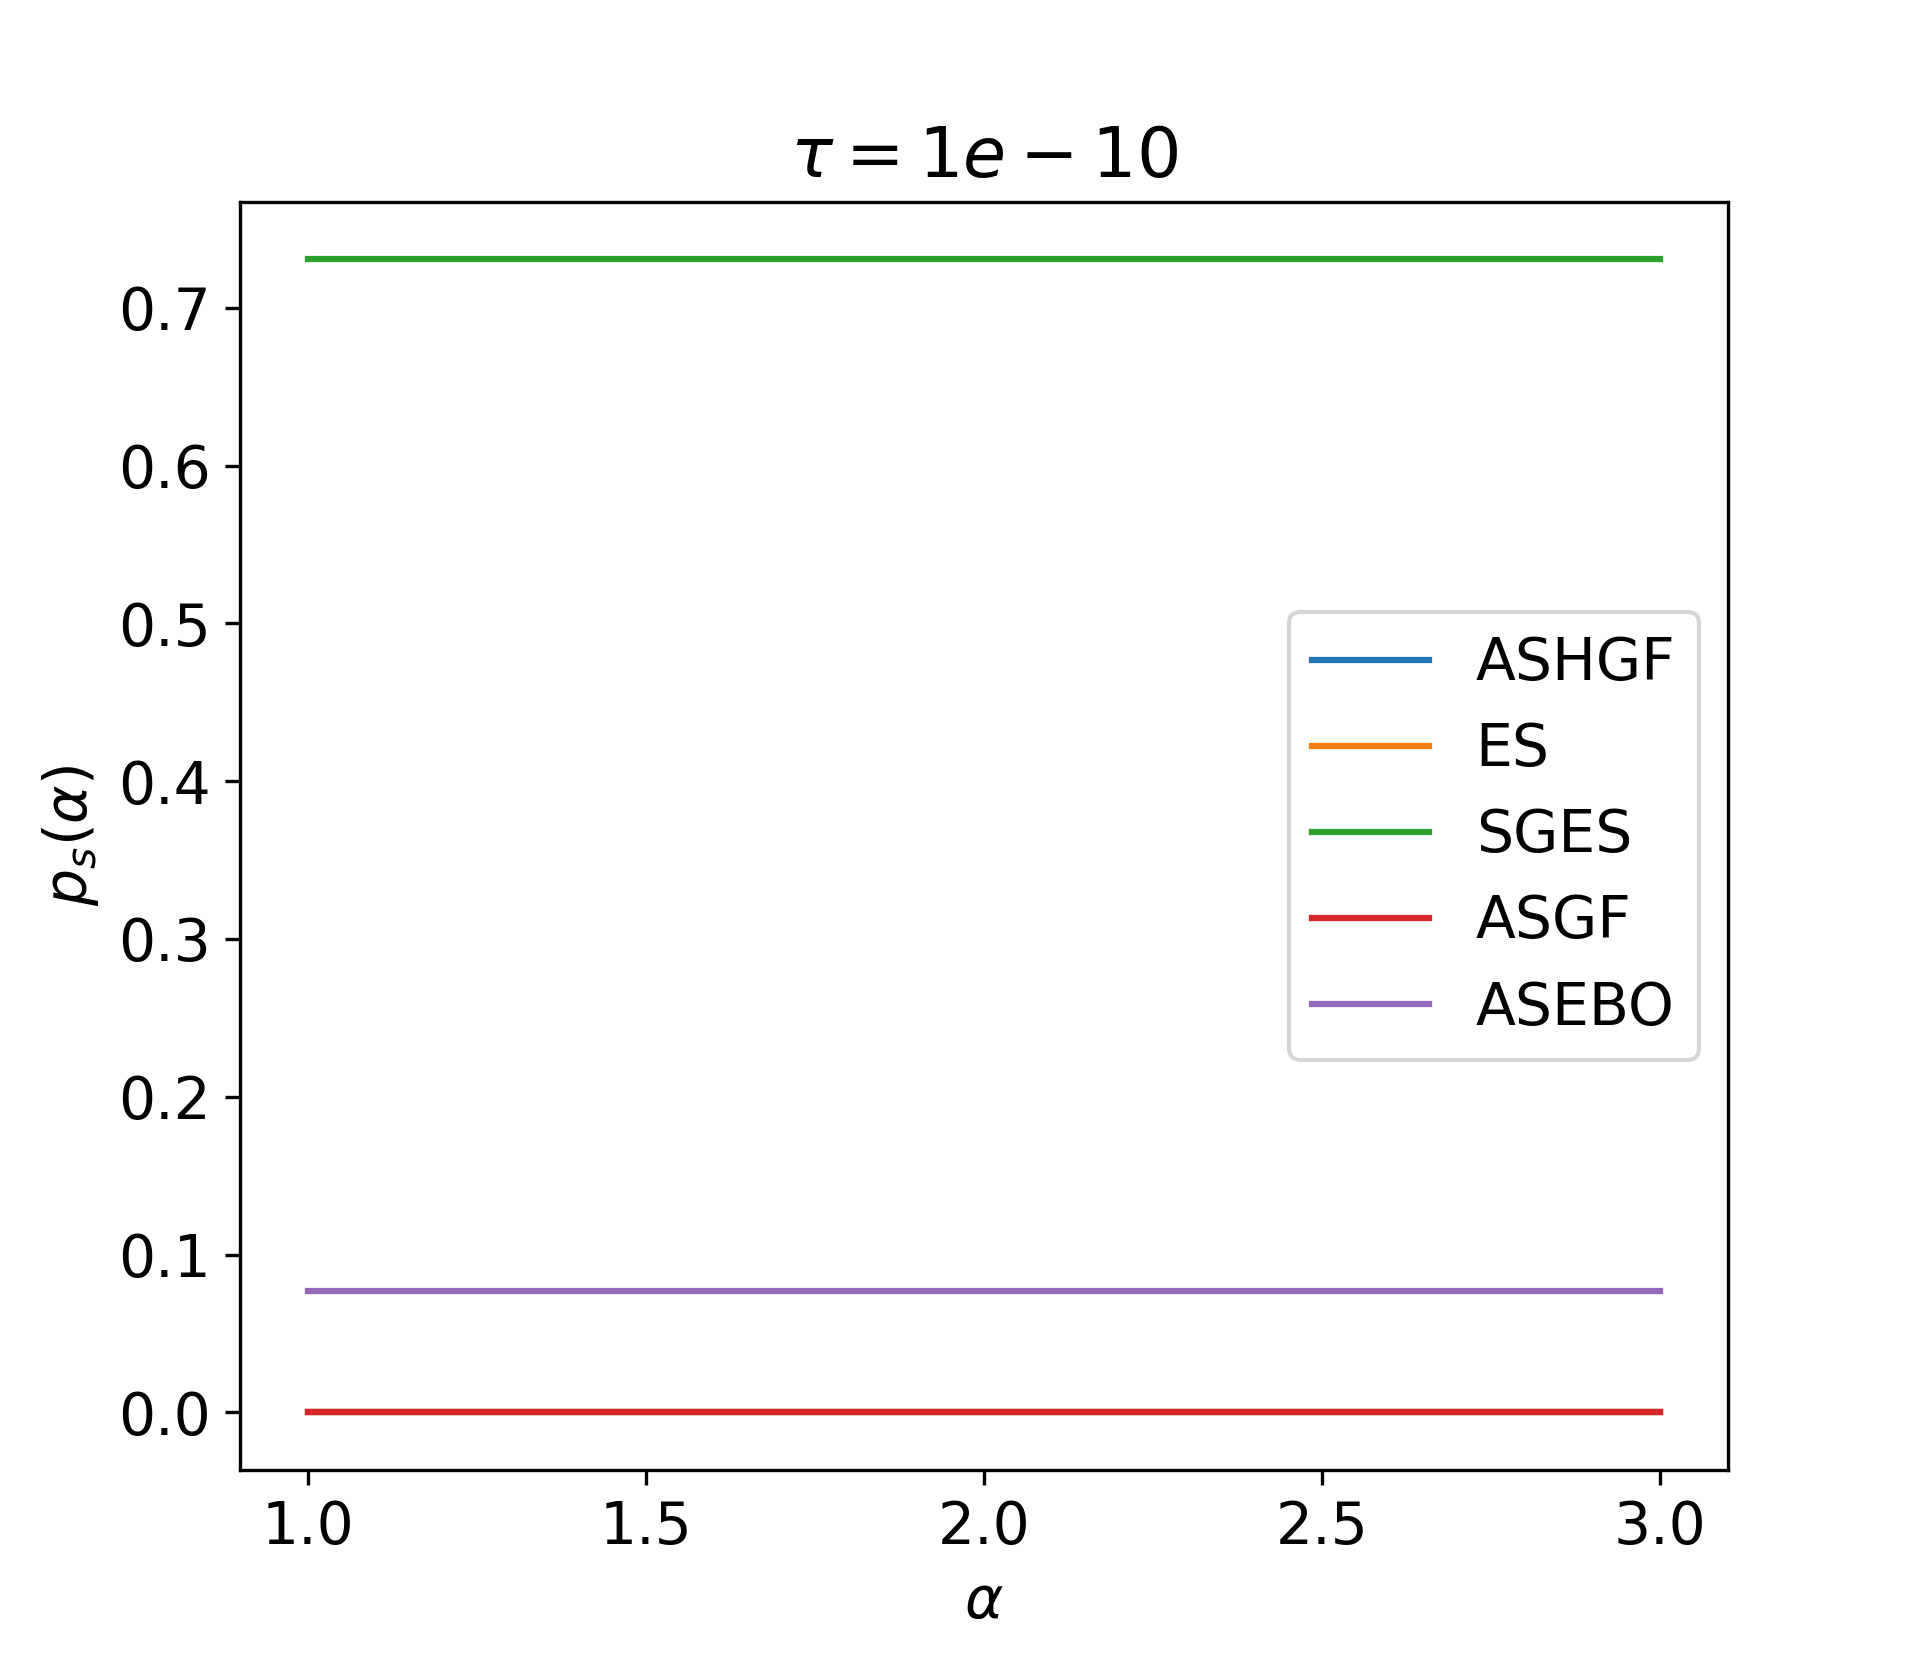
\includegraphics[width=1\textwidth]{figures/performance_profiles/1000/performance_profile_1000_10000_1e-10.png}
\end{subfigure}
\caption{Performance profiles with $\mu_L = 10^{4}$}
\label{PerformanceProfiles1000Mu10000}
\end{figure}

\begin{figure}[H]
\centering
\begin{subfigure}{0.3\textwidth}
  \centering 
  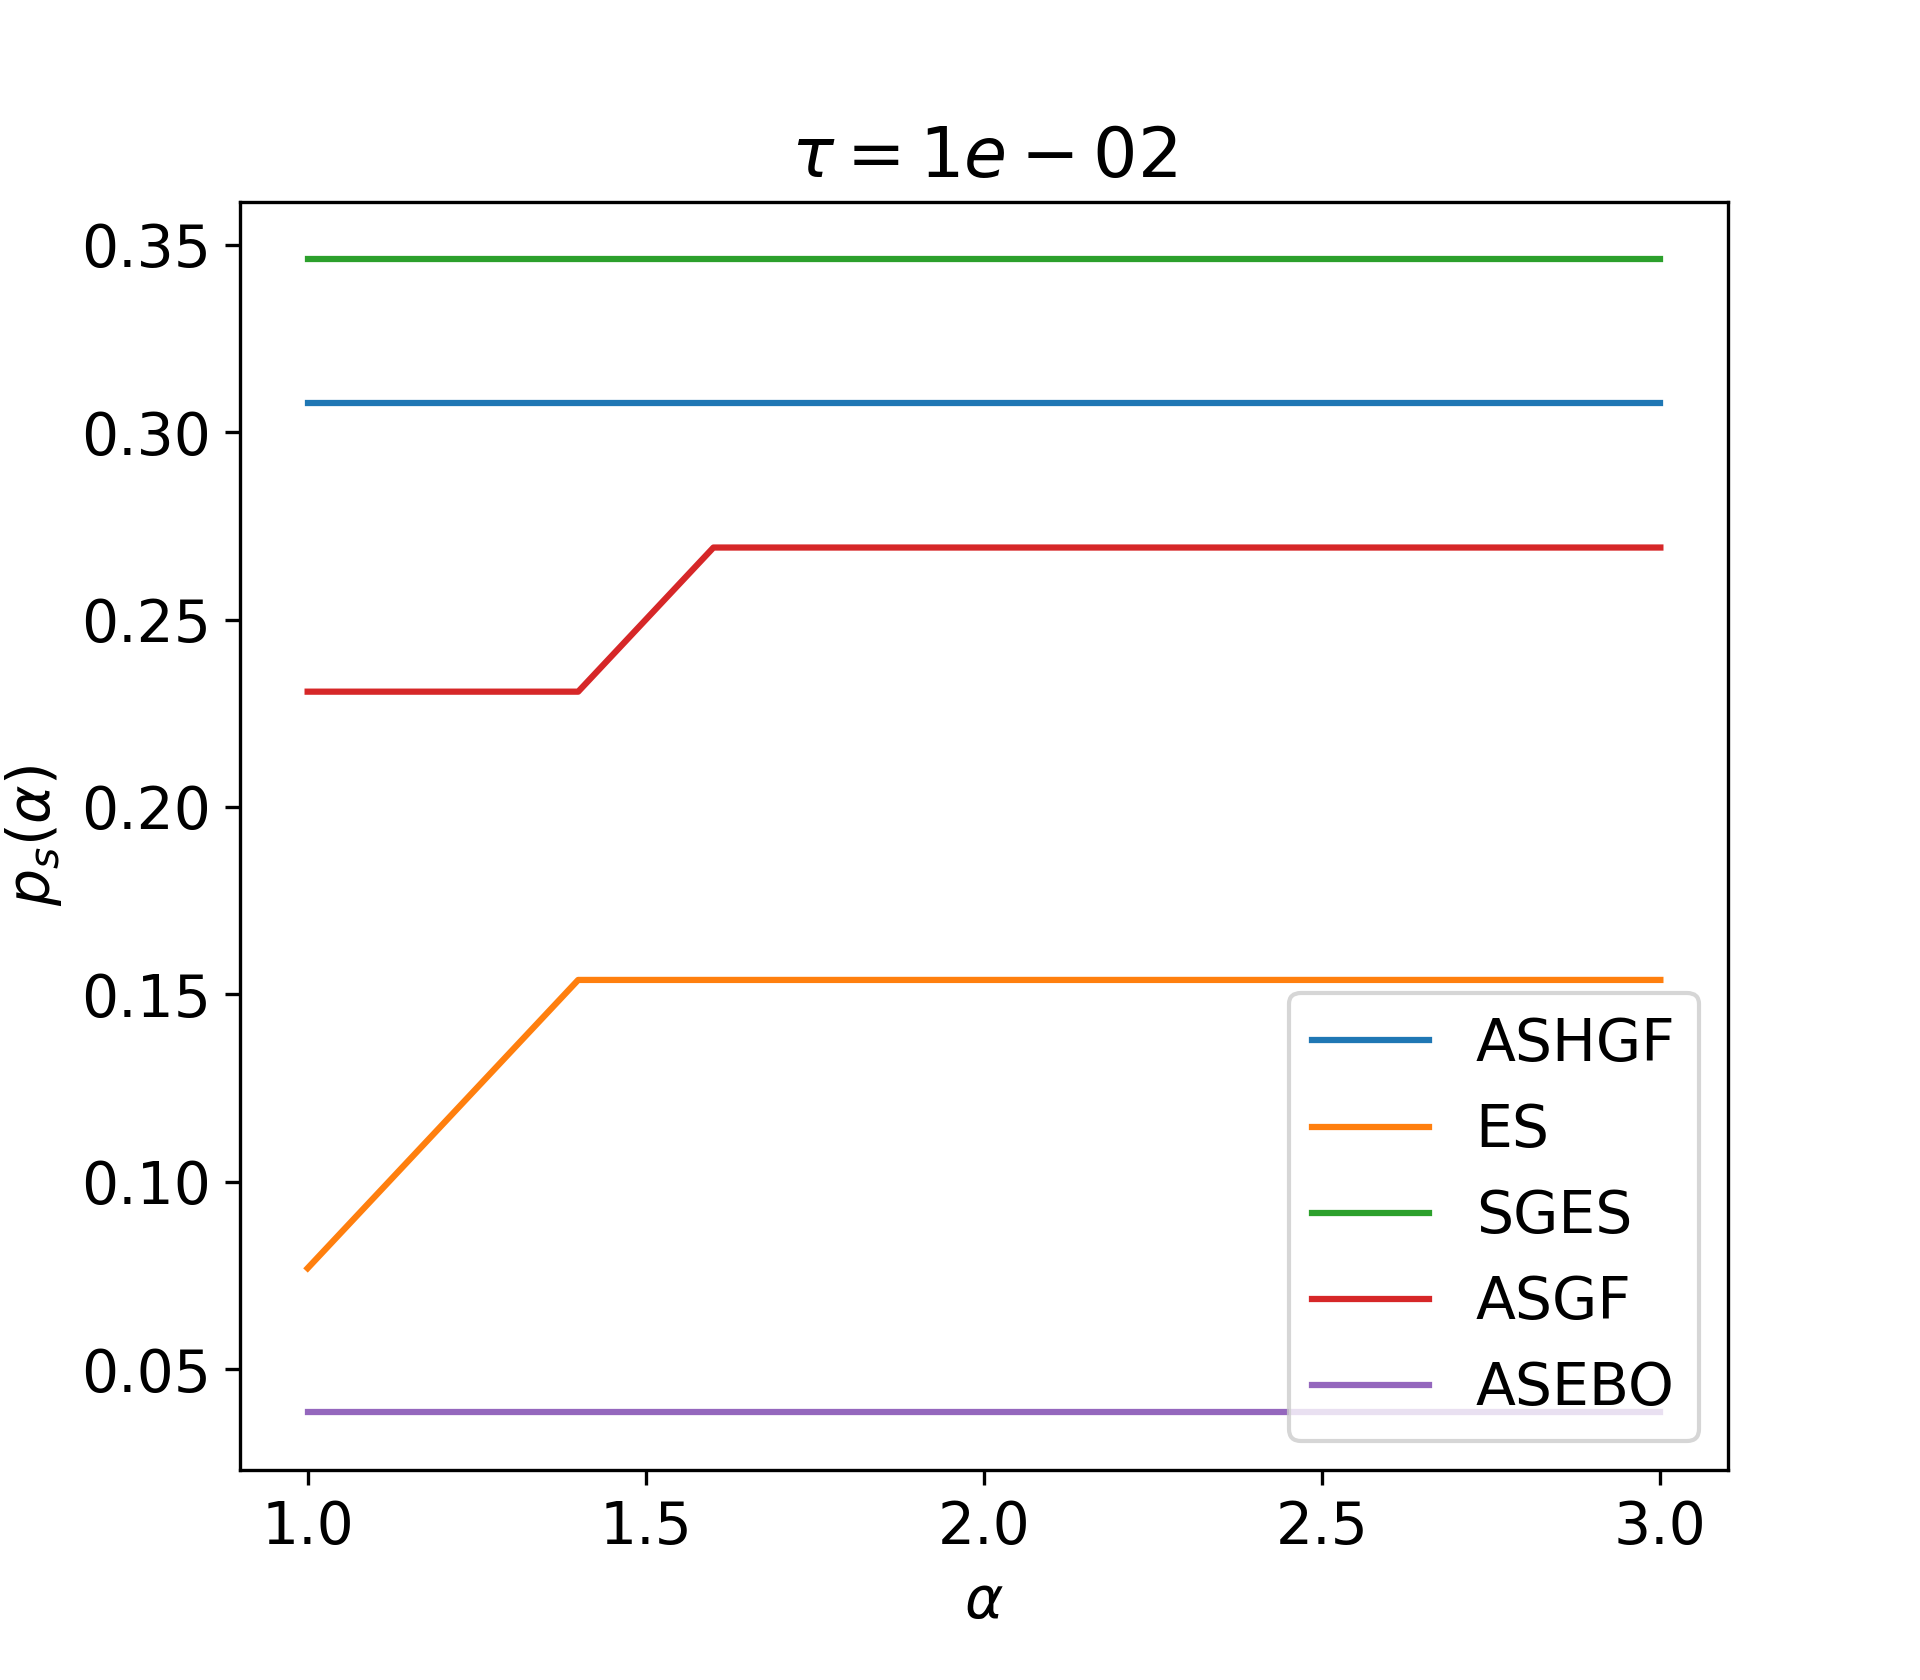
\includegraphics[width=1\textwidth]{figures/performance_profiles/1000/performance_profile_1000_100000_1e-02.png}
\end{subfigure}%
\begin{subfigure}{0.3\textwidth}
  \centering 
  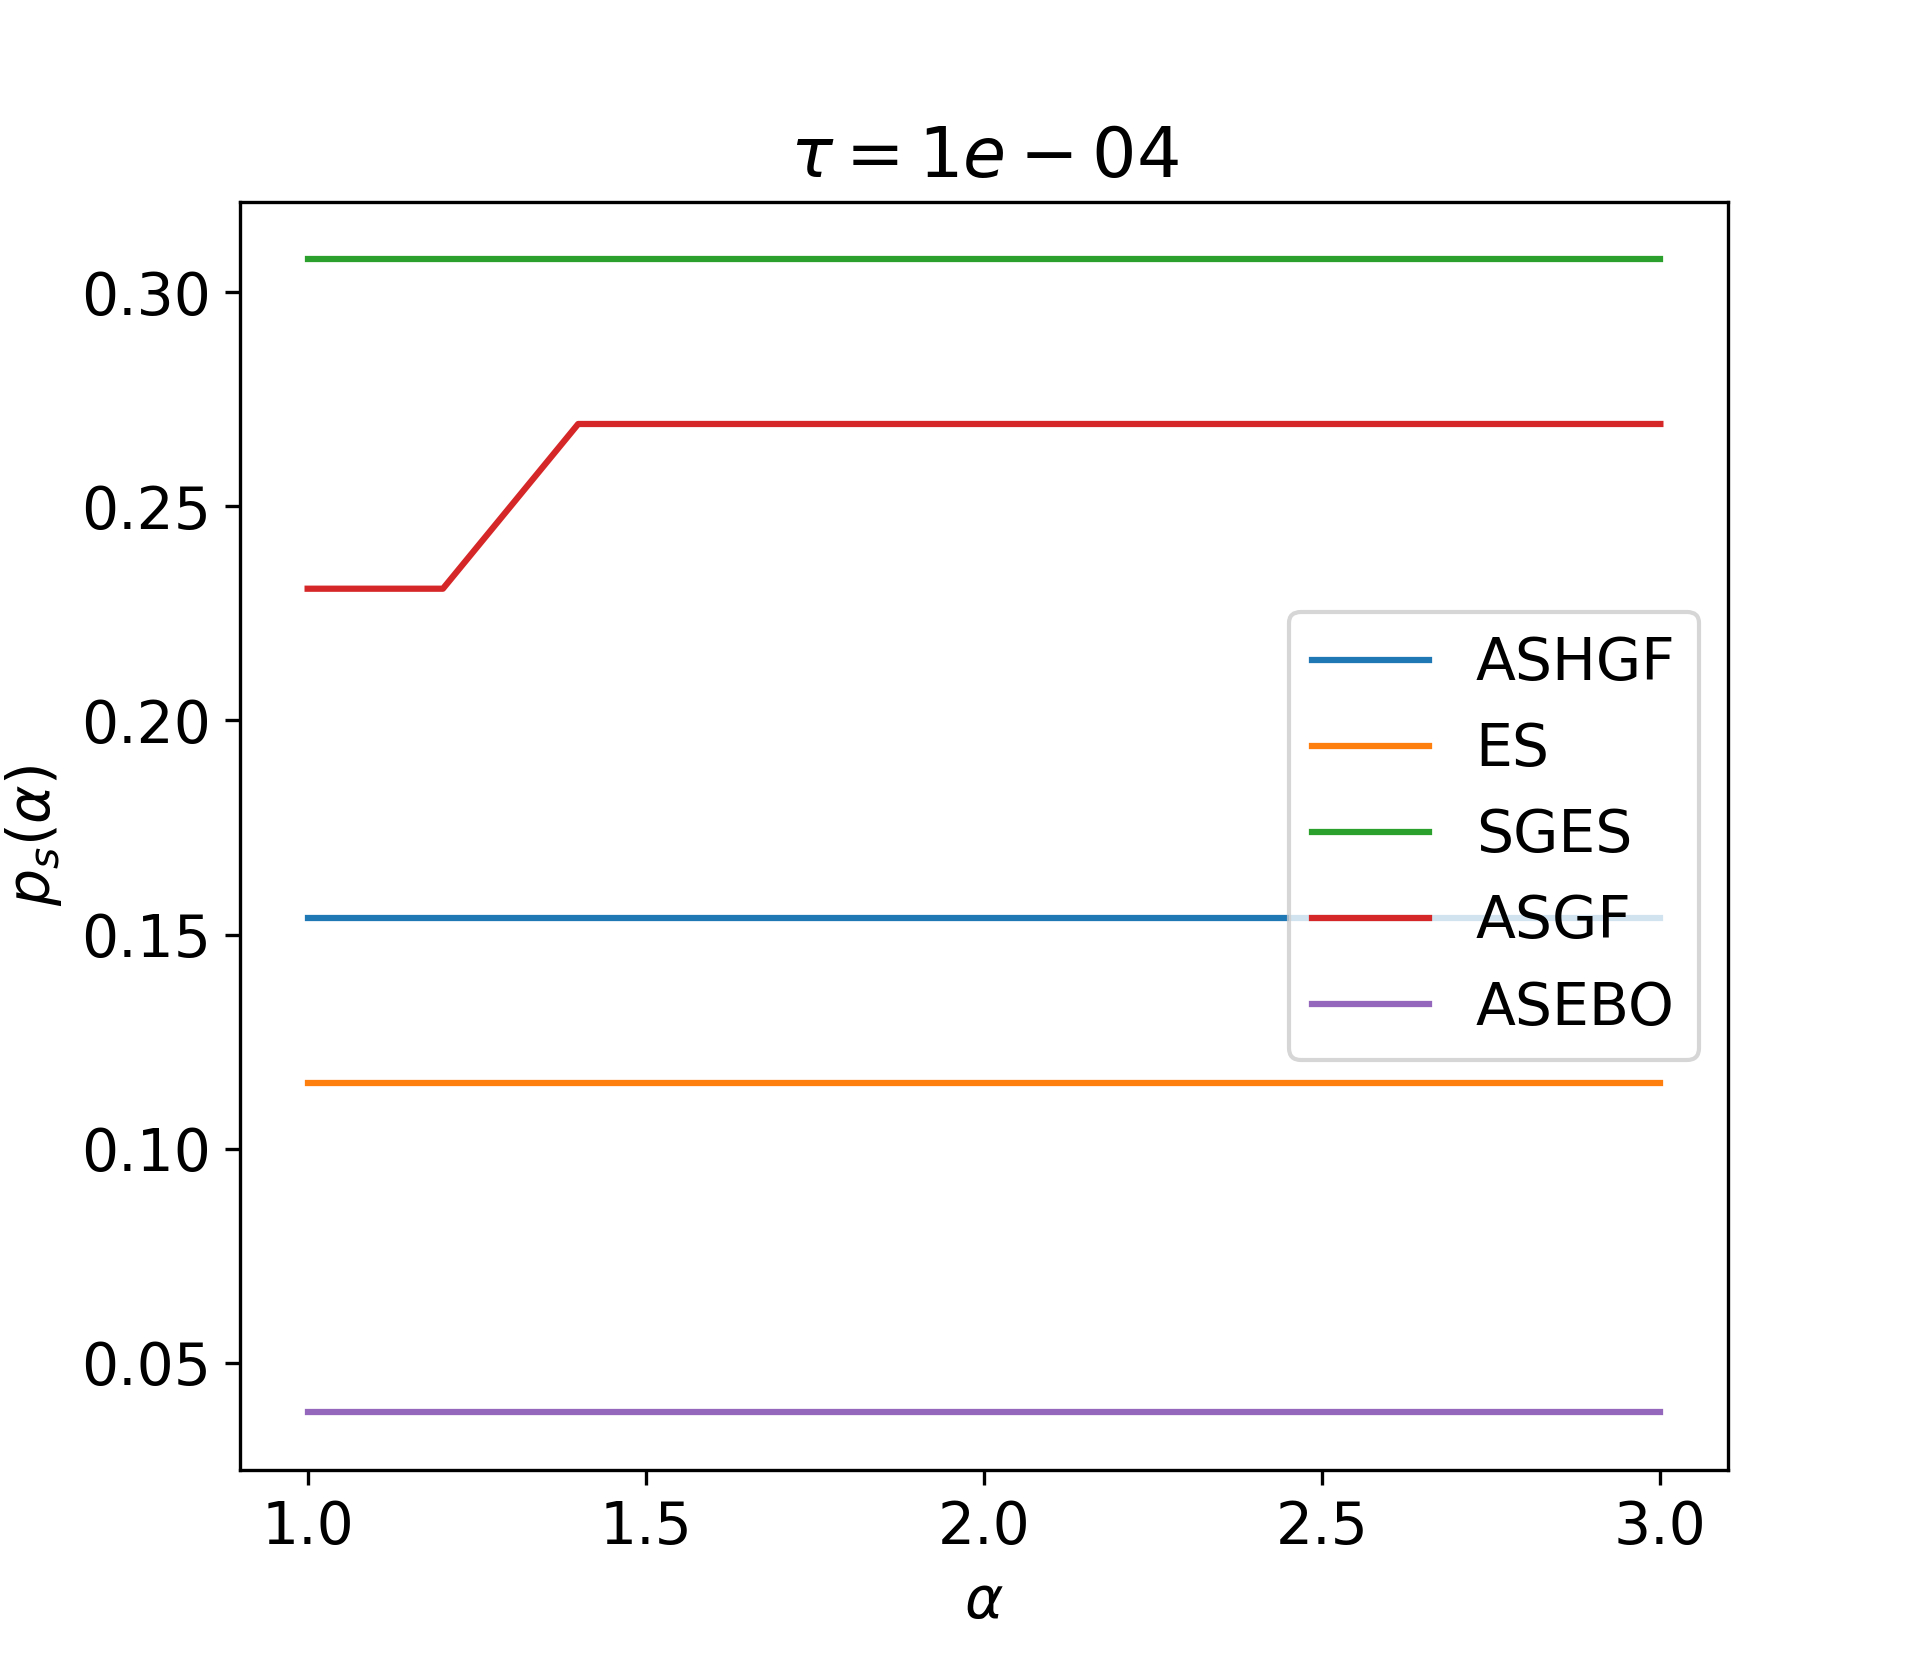
\includegraphics[width=1\textwidth]{figures/performance_profiles/1000/performance_profile_1000_100000_1e-04.png}
\end{subfigure}
\begin{subfigure}{0.3\textwidth}
  \centering 
  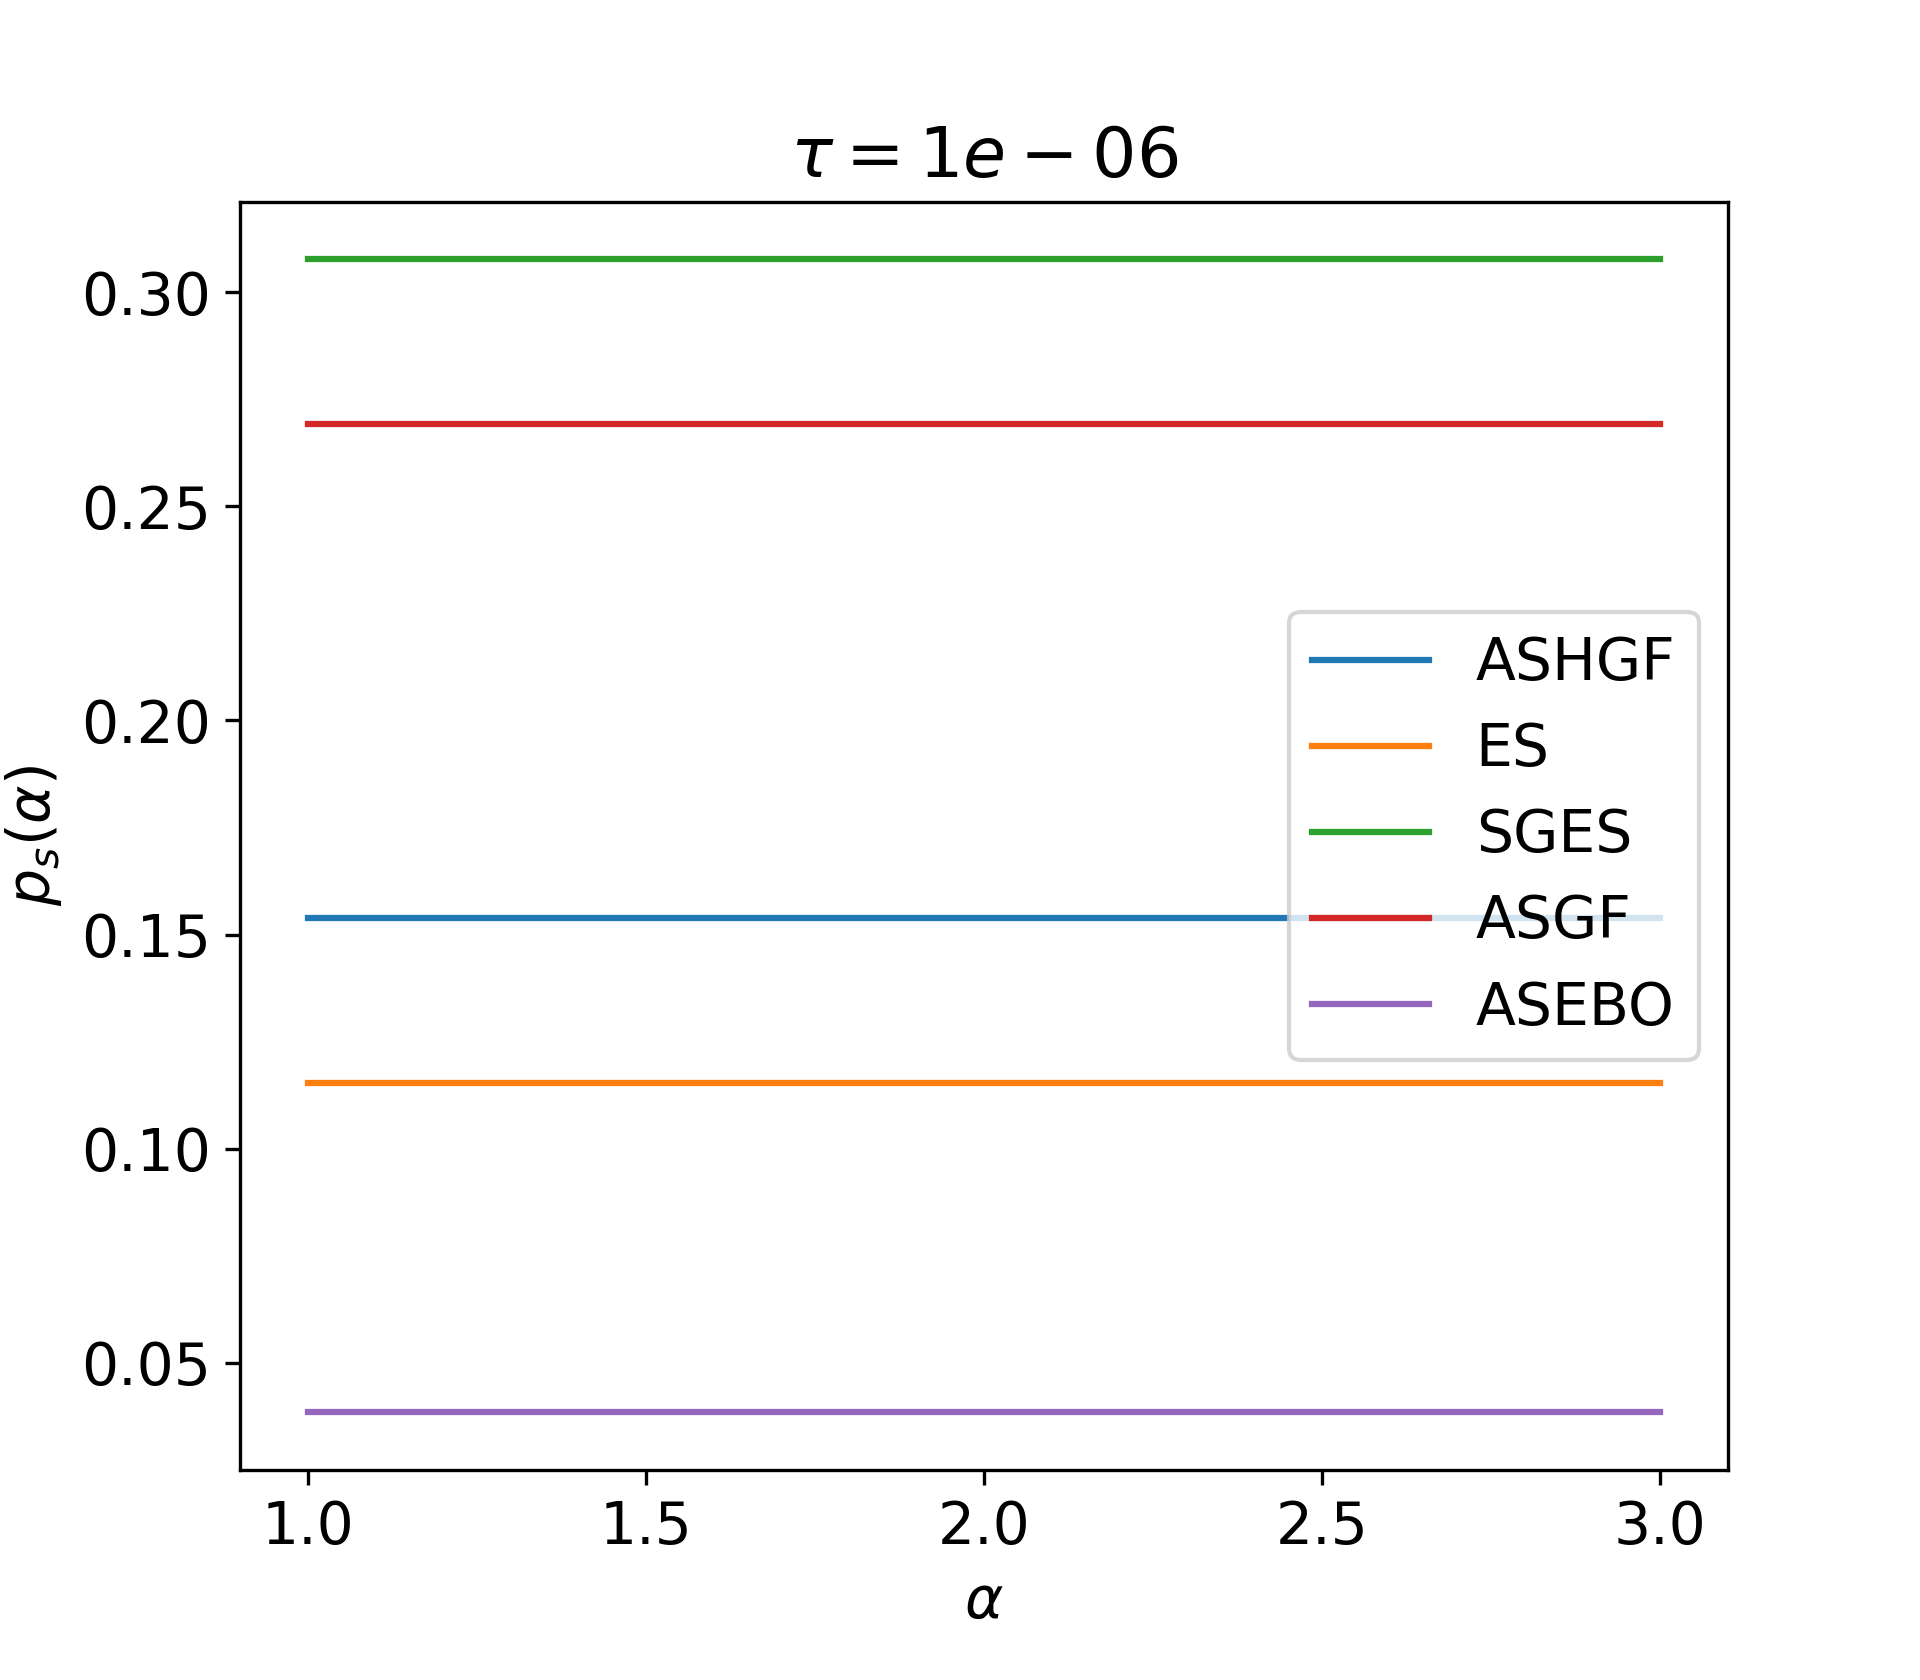
\includegraphics[width=1\textwidth]{figures/performance_profiles/1000/performance_profile_1000_100000_1e-06.png}
\end{subfigure}
\centering
\begin{subfigure}{0.3\textwidth}
  \centering 
  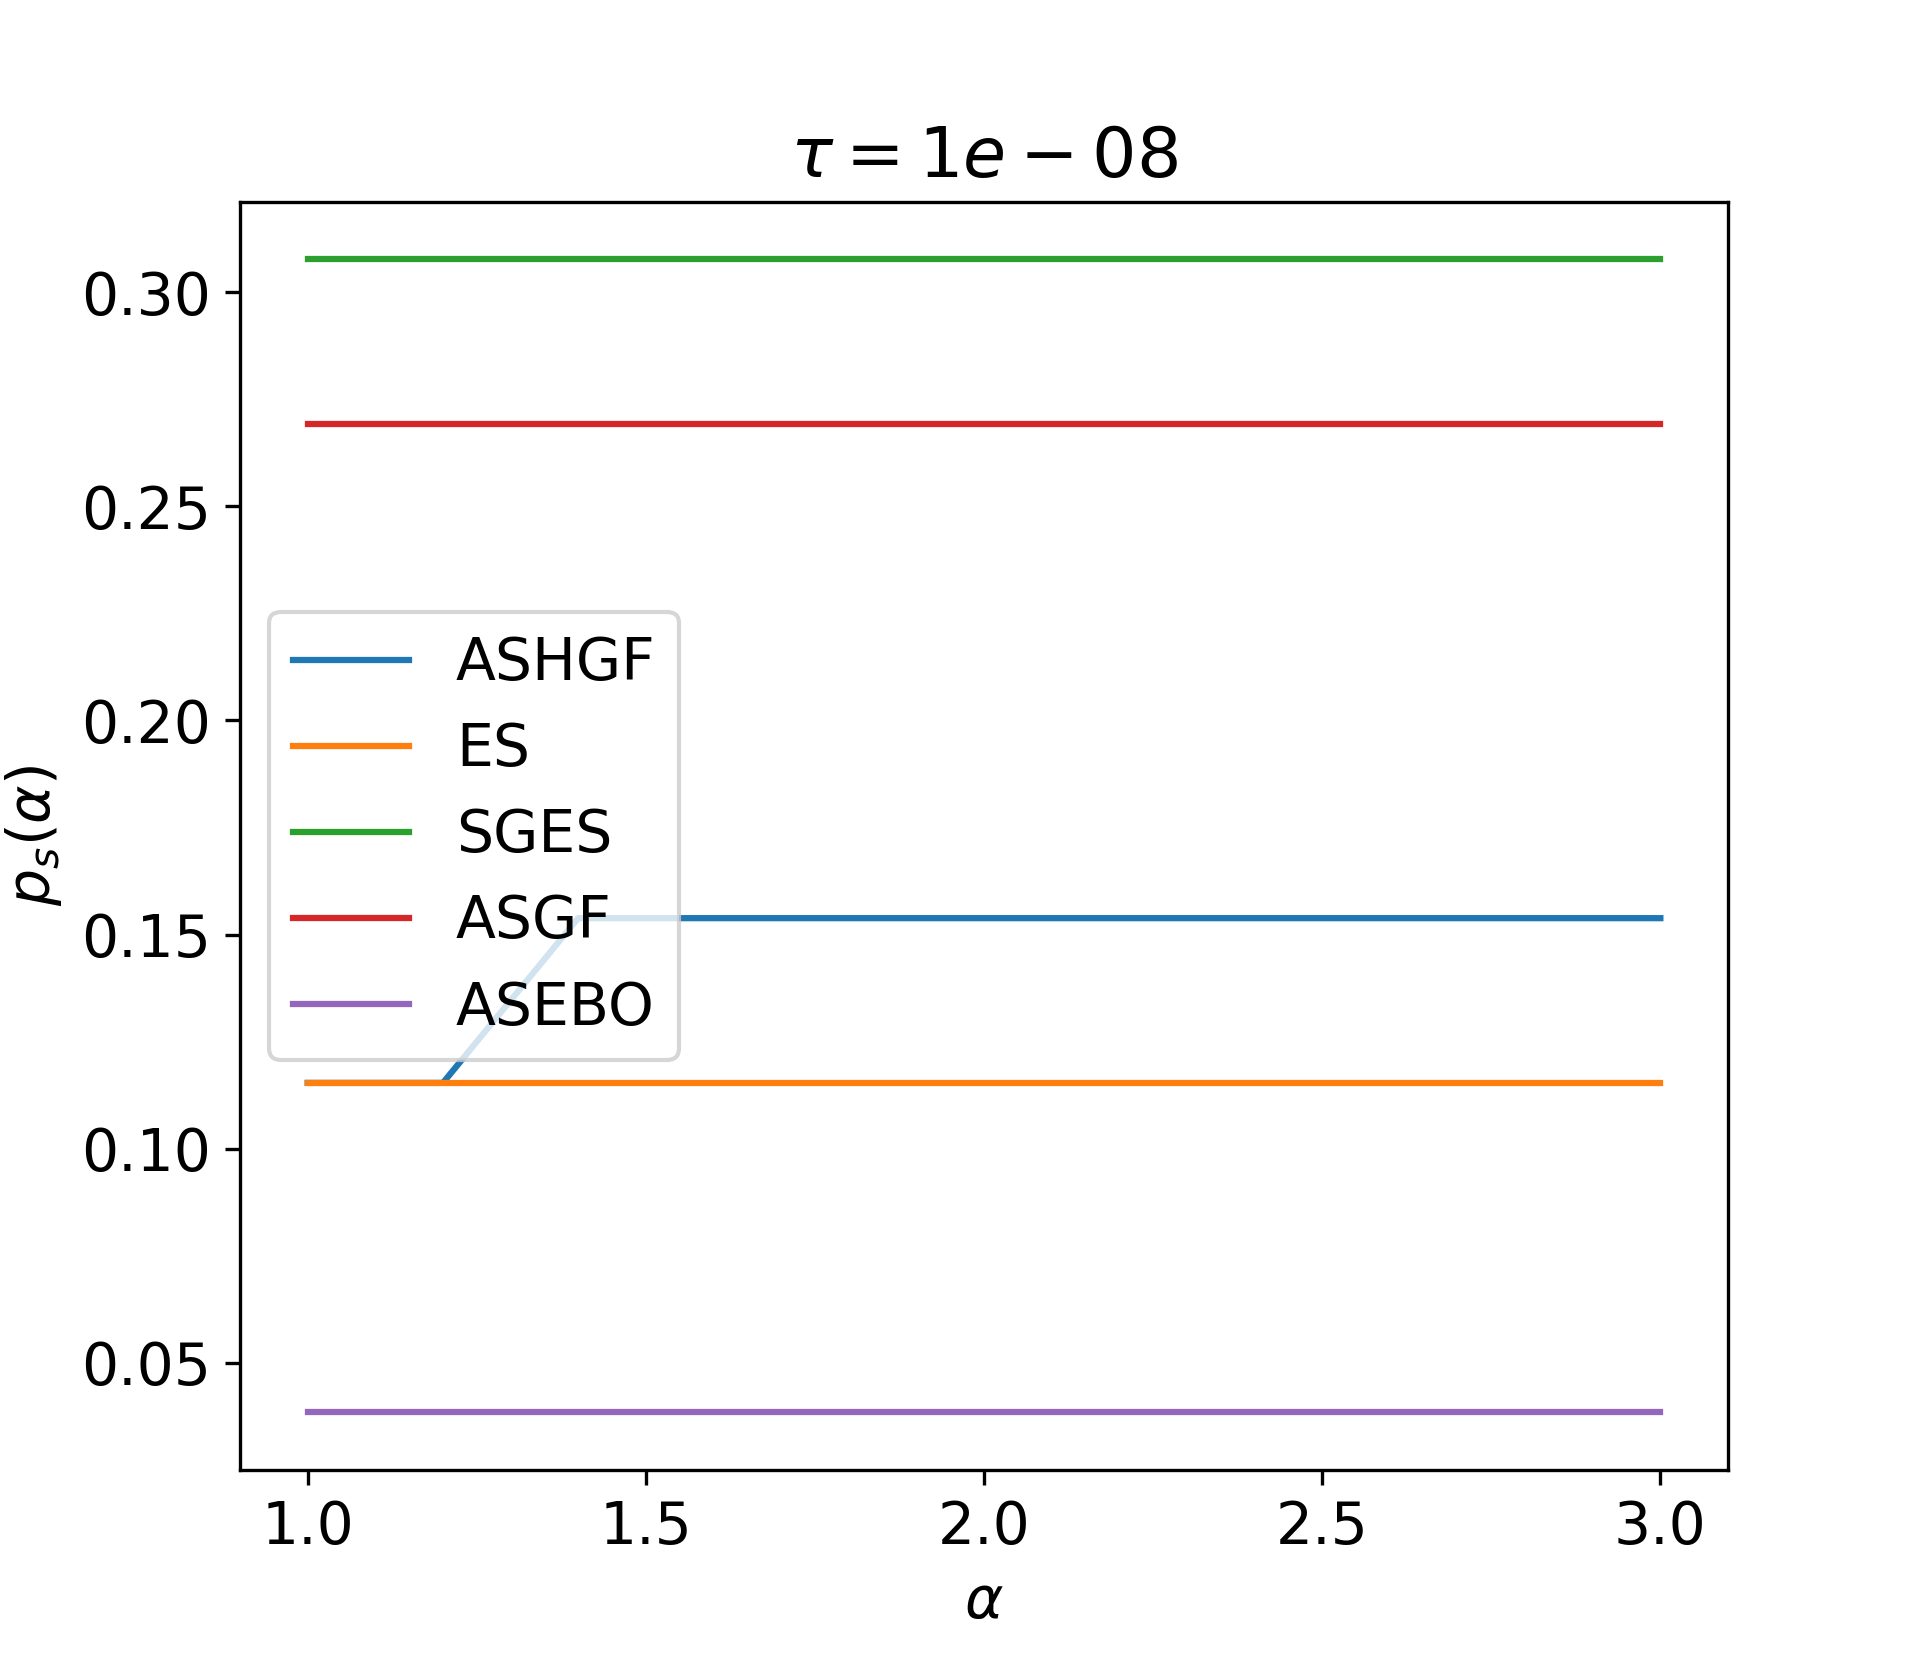
\includegraphics[width=1\textwidth]{figures/performance_profiles/1000/performance_profile_1000_100000_1e-08.png}
\end{subfigure}%
\begin{subfigure}{0.3\textwidth}
  \centering 
  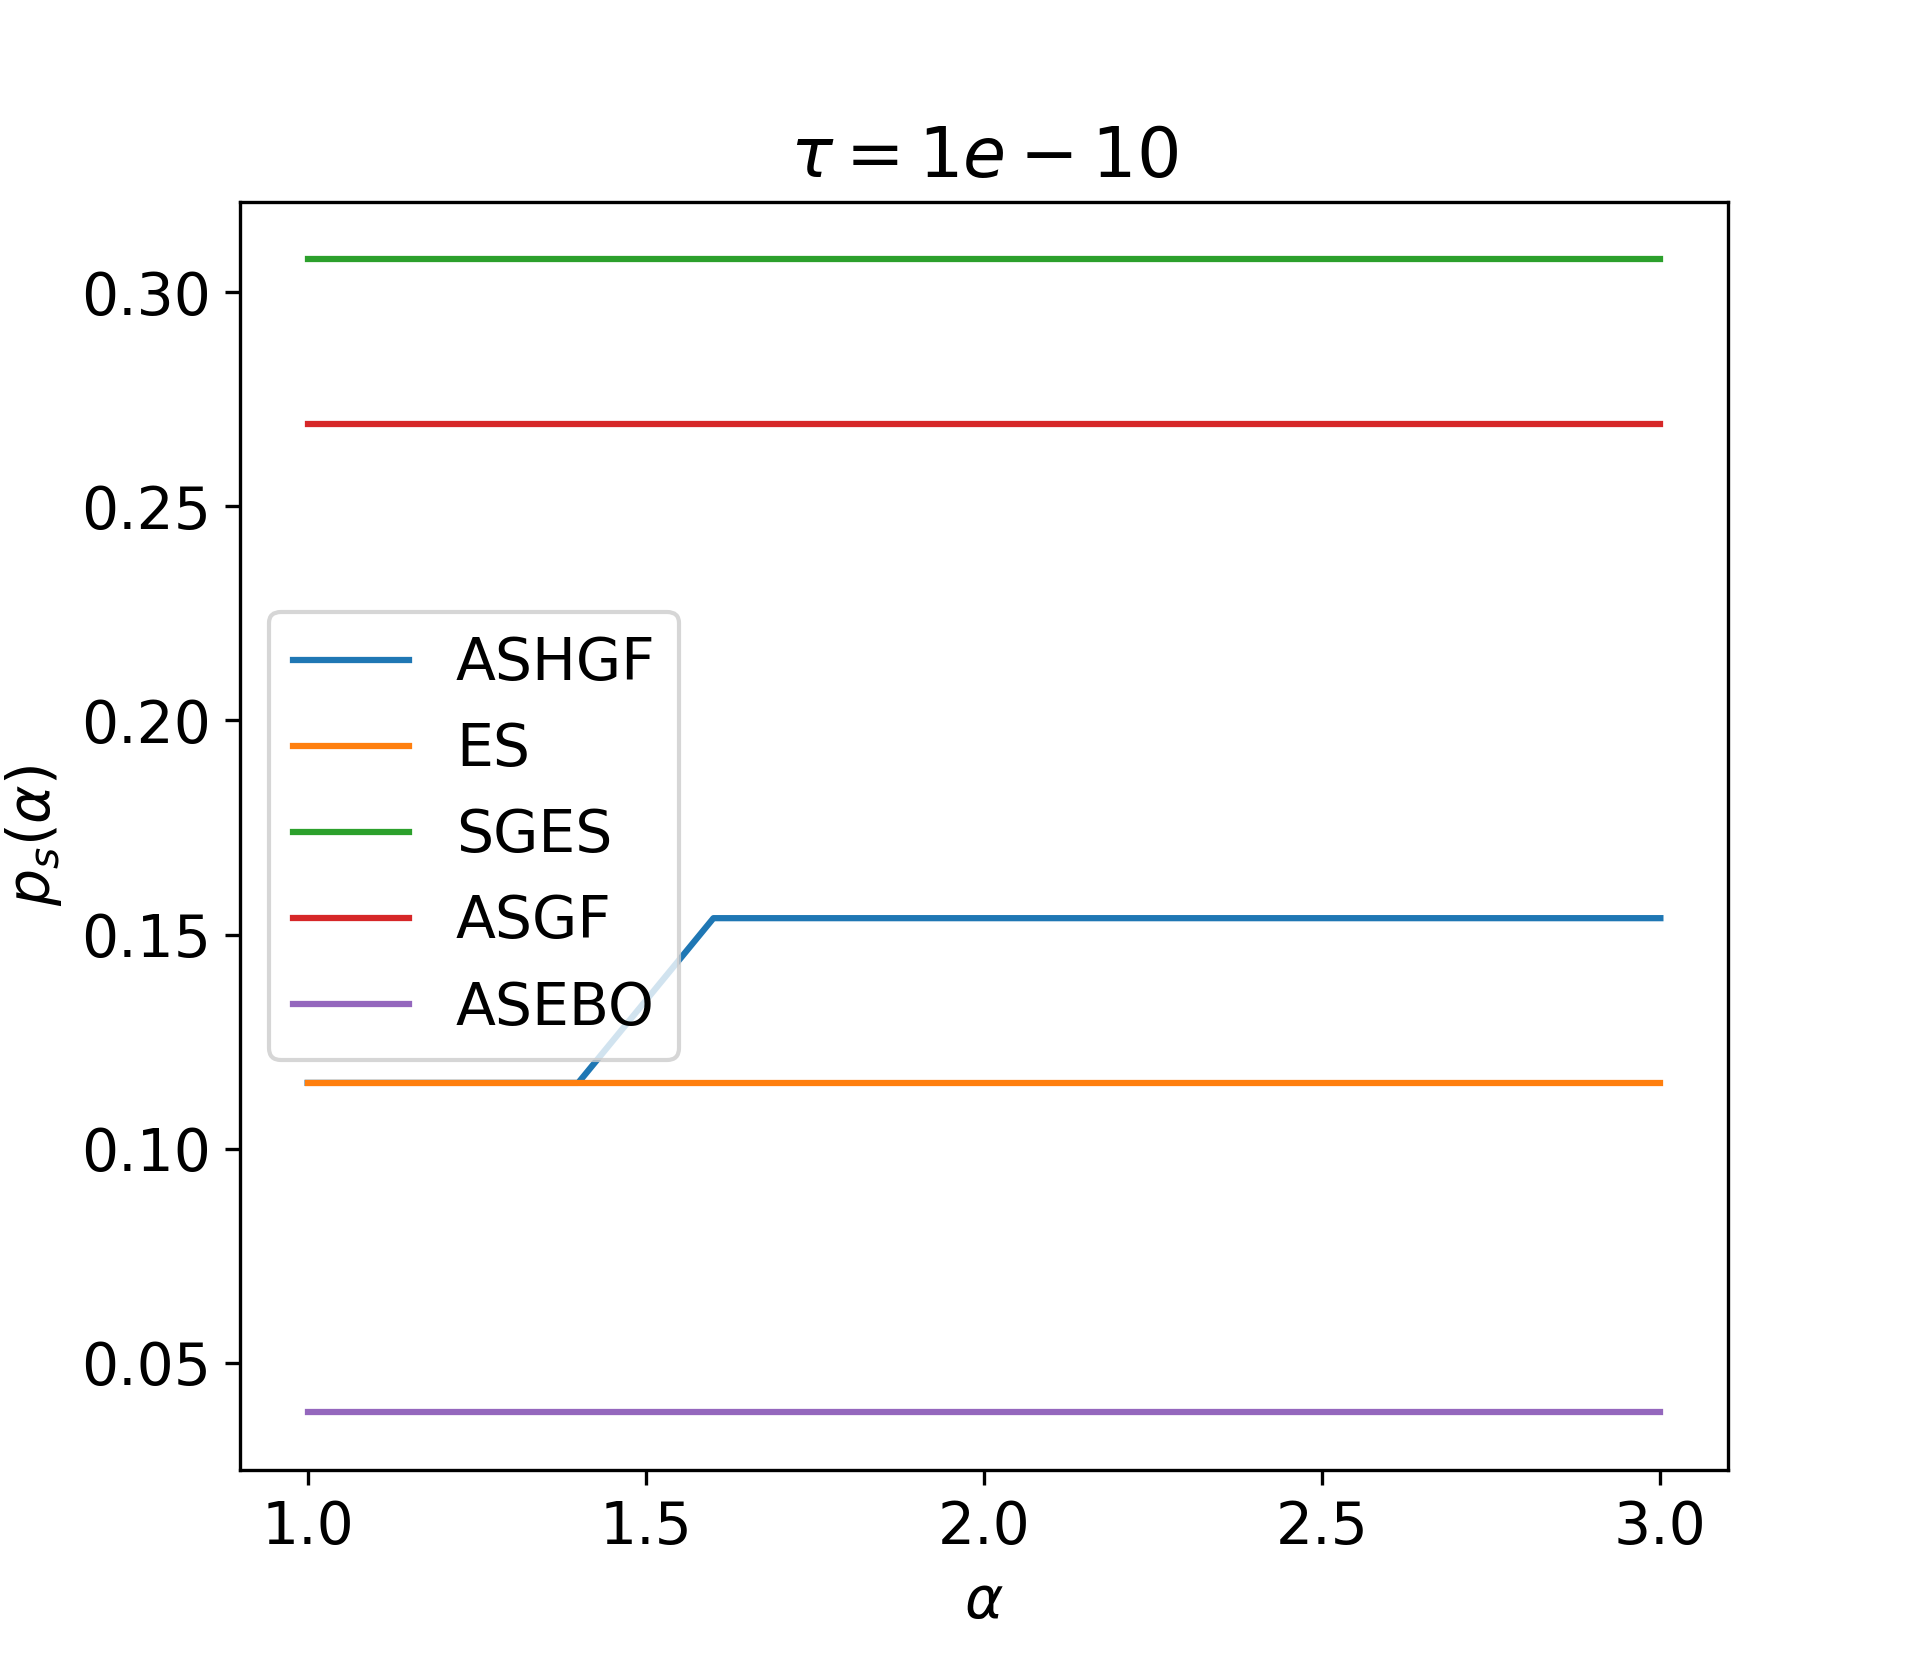
\includegraphics[width=1\textwidth]{figures/performance_profiles/1000/performance_profile_1000_100000_1e-10.png}
\end{subfigure}
\caption{Performance profiles with $\mu_L = 10^{5}$}
\label{PerformanceProfiles1000Mu100000}
\end{figure}

\begin{figure}[H]
\centering
\begin{subfigure}{0.3\textwidth}
  \centering 
  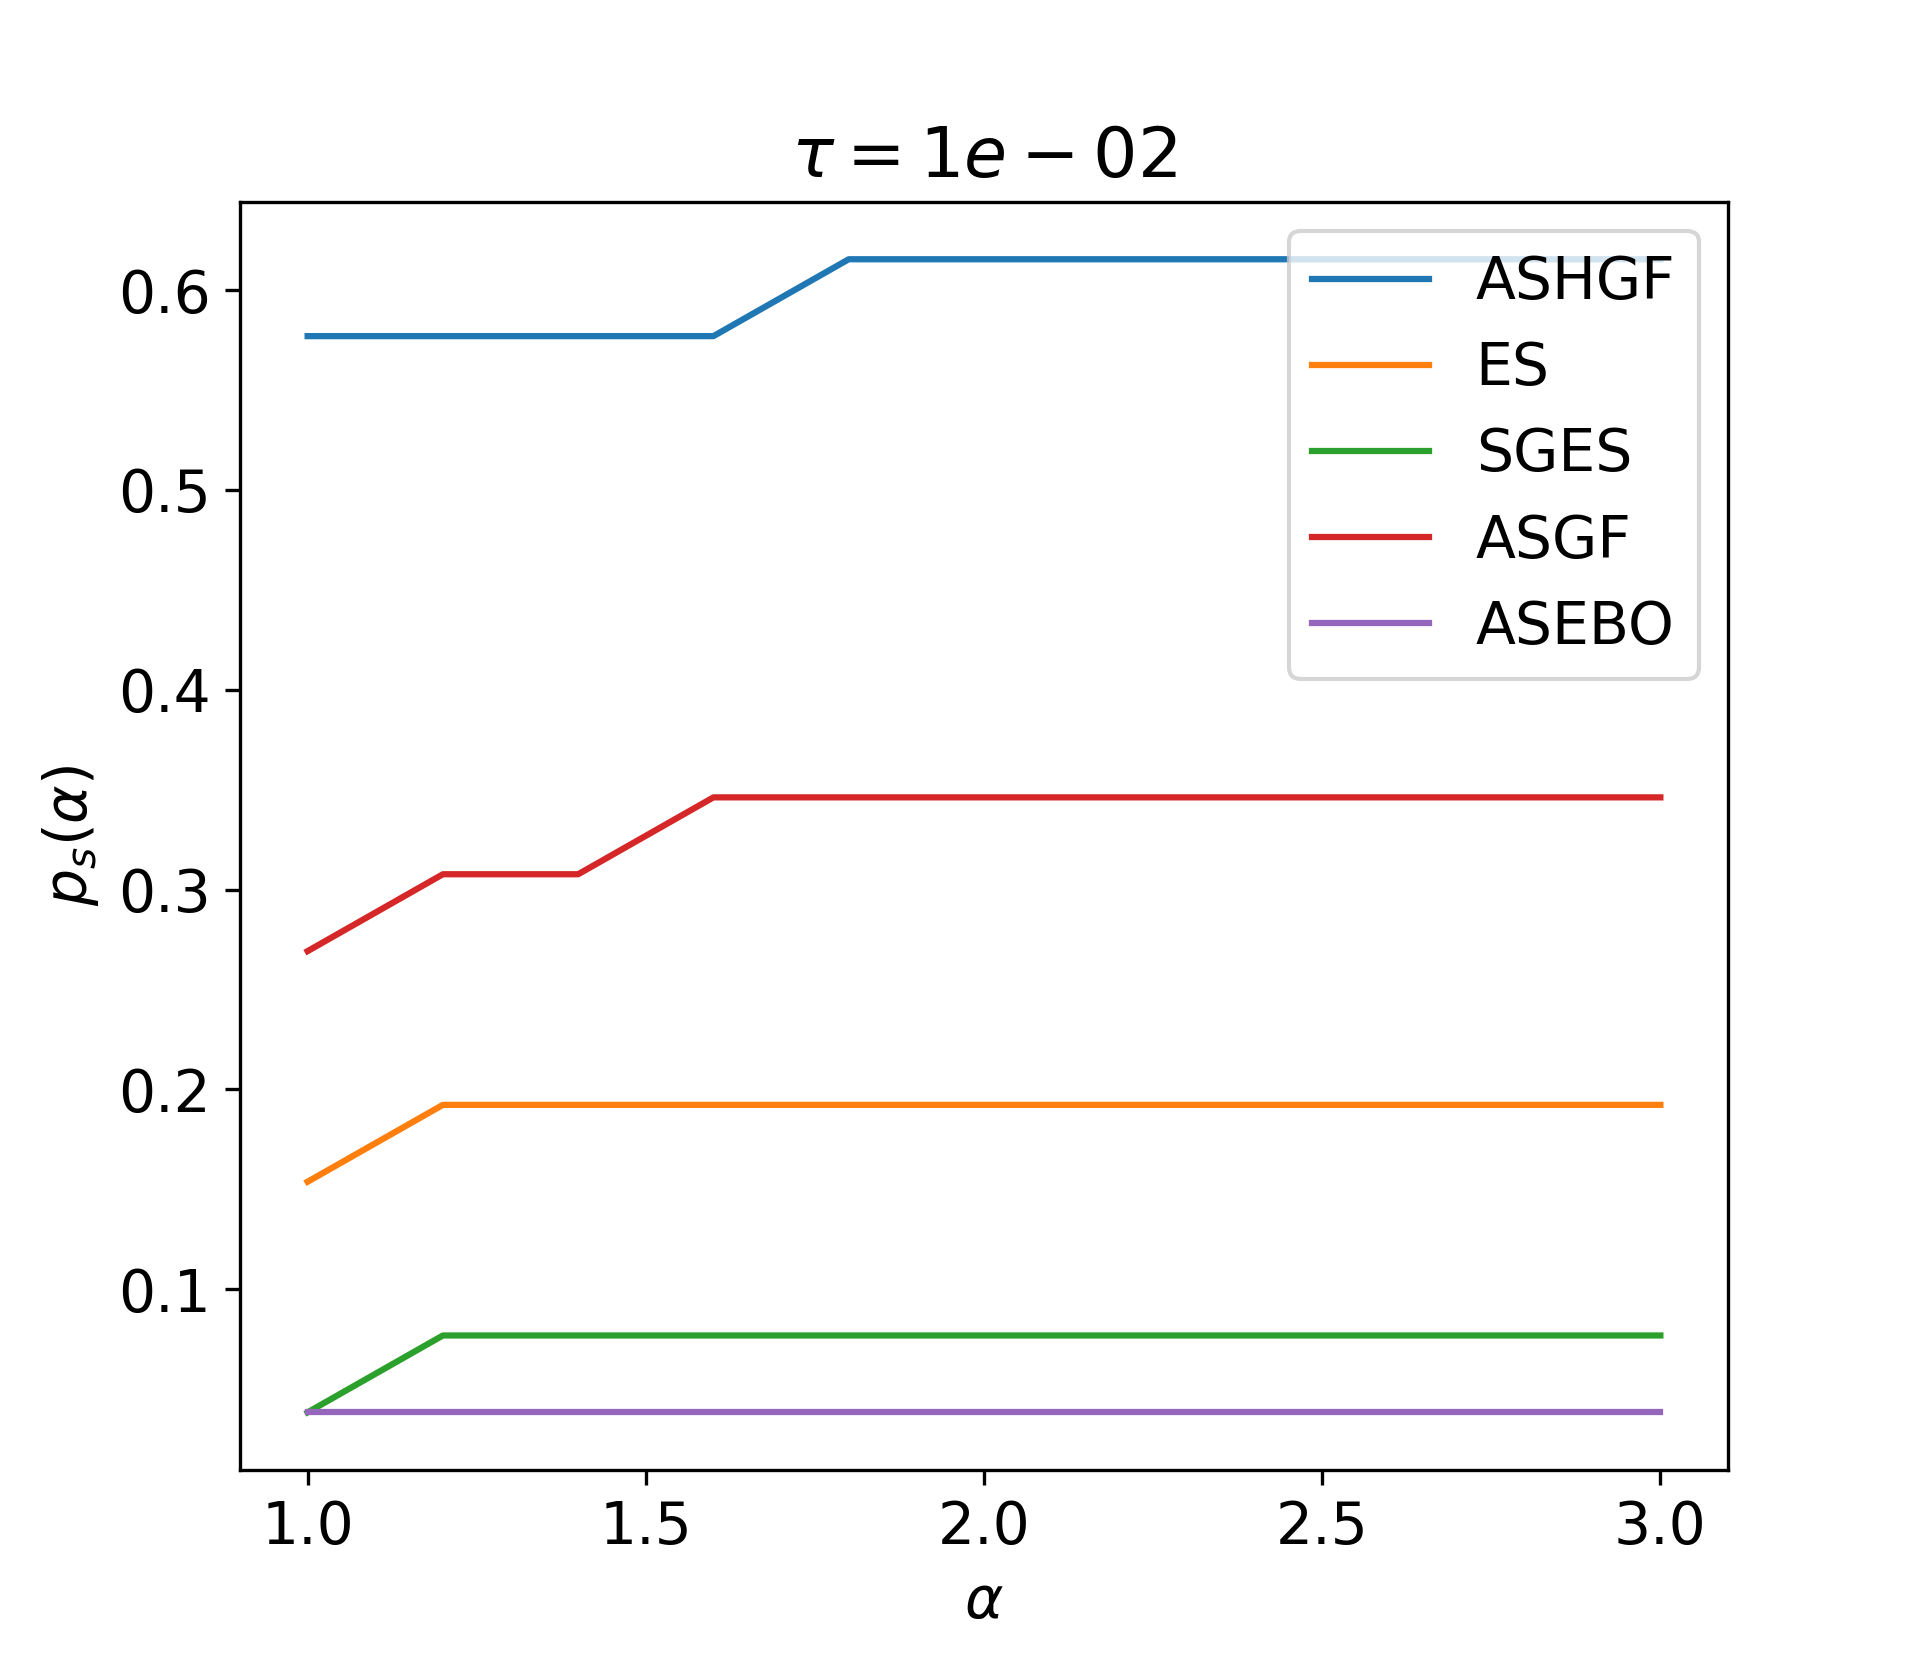
\includegraphics[width=1\textwidth]{figures/performance_profiles/1000/performance_profile_1000_1000000_1e-02.png}
\end{subfigure}%
\begin{subfigure}{0.3\textwidth}
  \centering 
  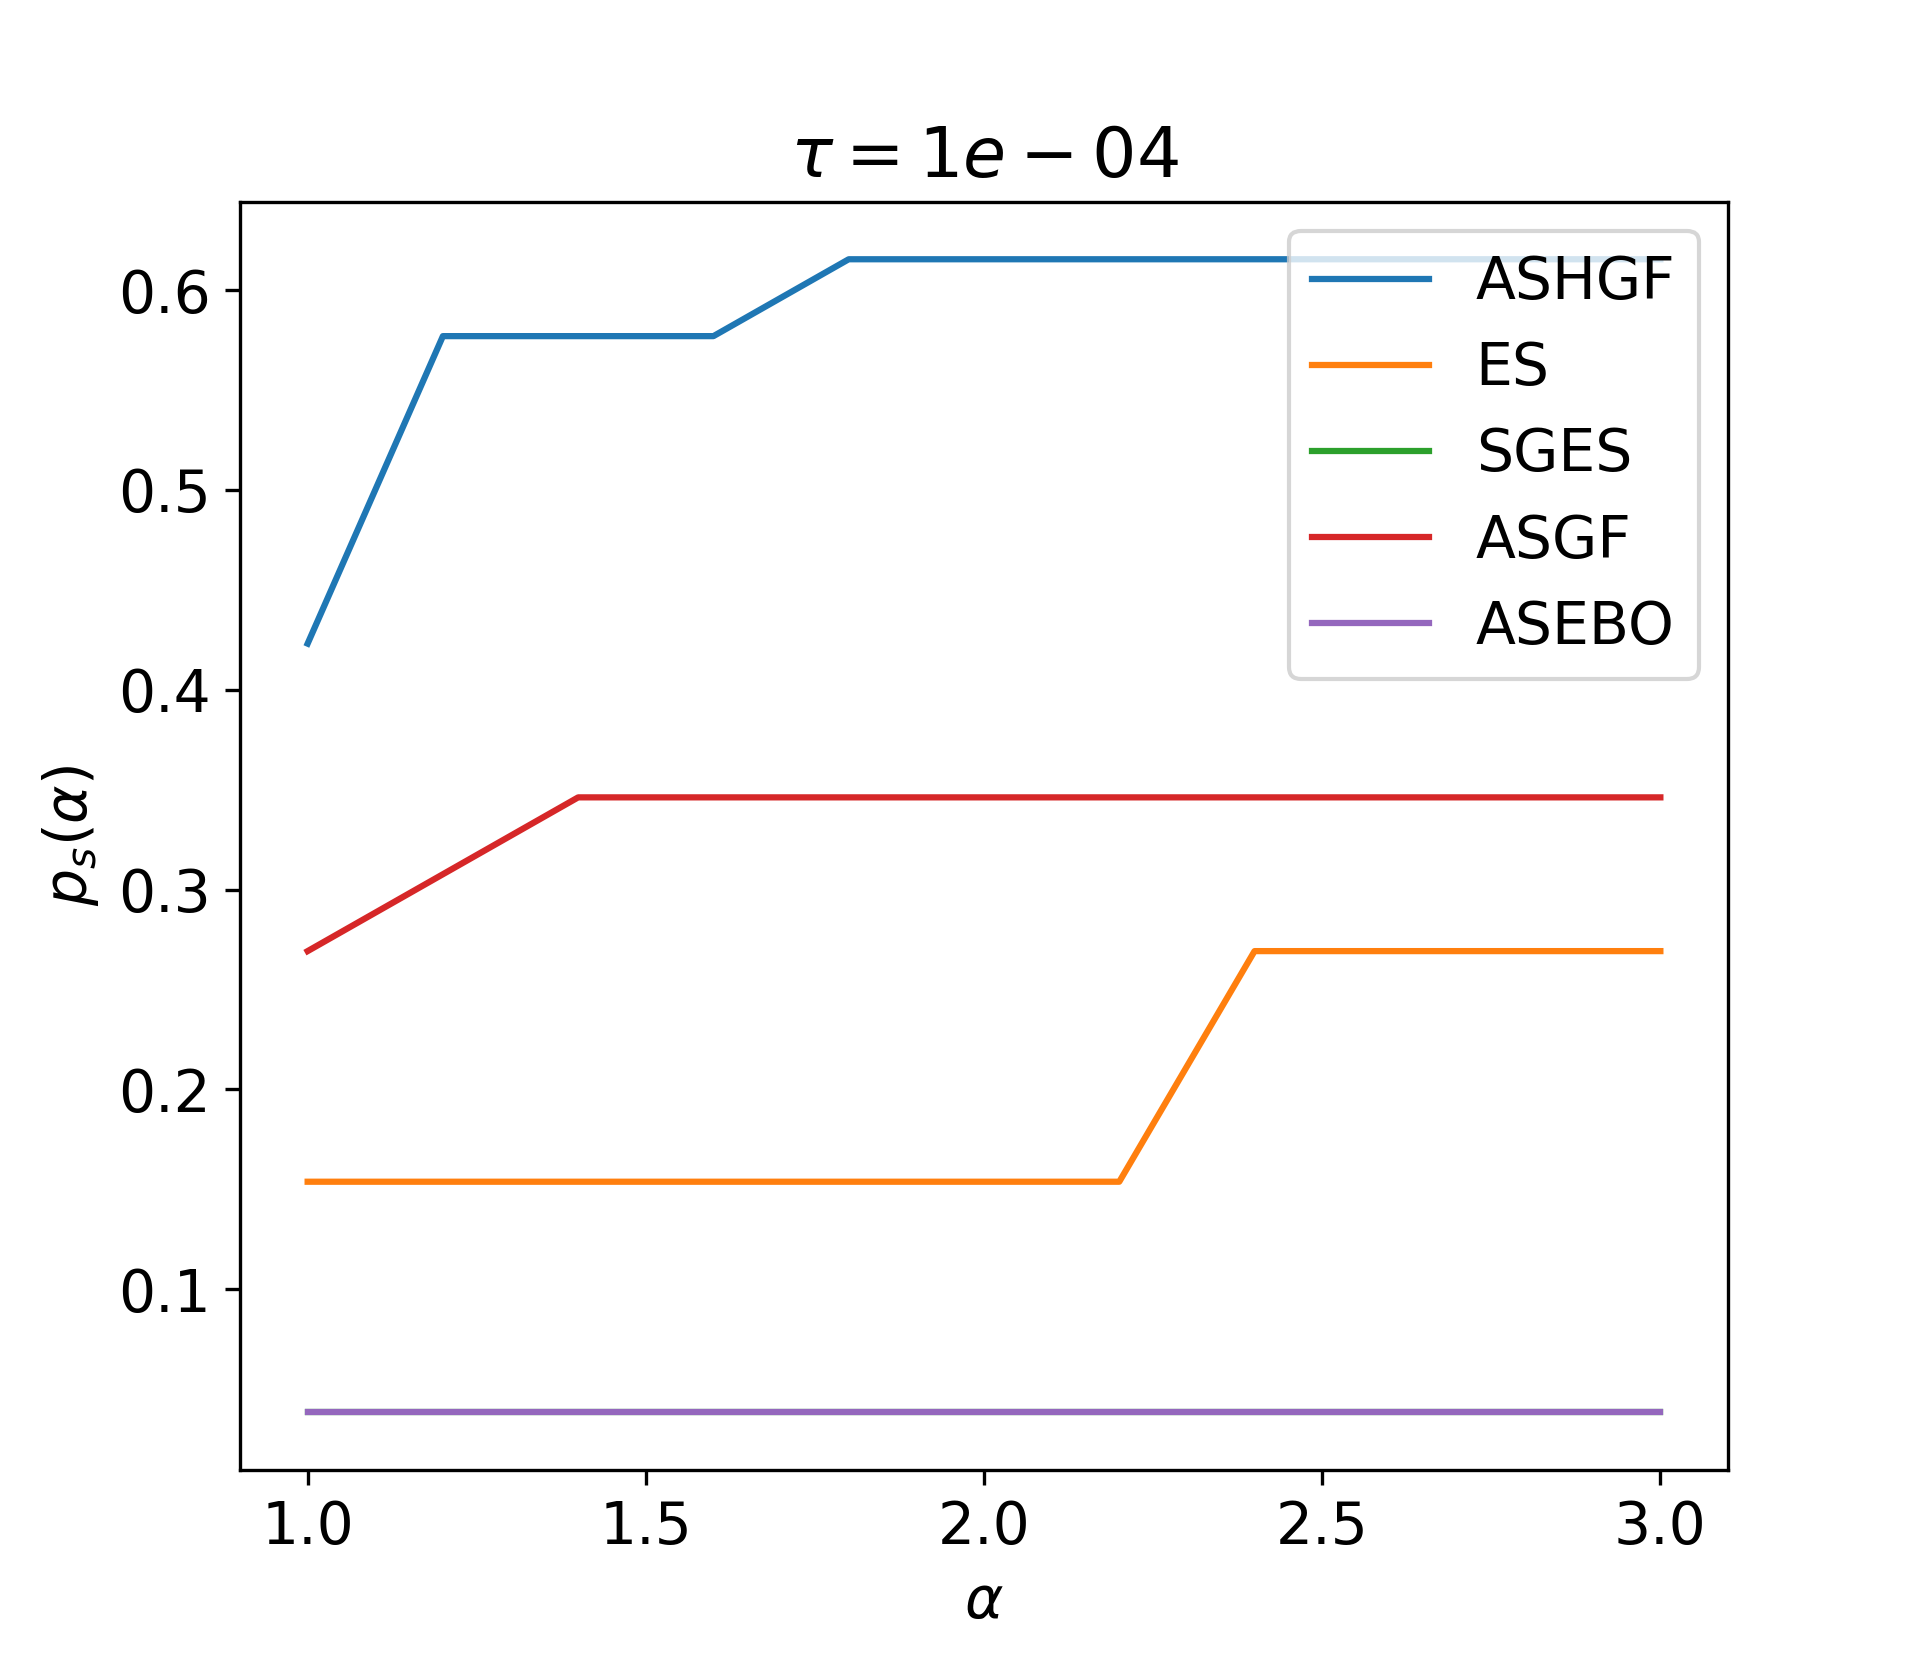
\includegraphics[width=1\textwidth]{figures/performance_profiles/1000/performance_profile_1000_1000000_1e-04.png}
\end{subfigure}
\begin{subfigure}{0.3\textwidth}
  \centering 
  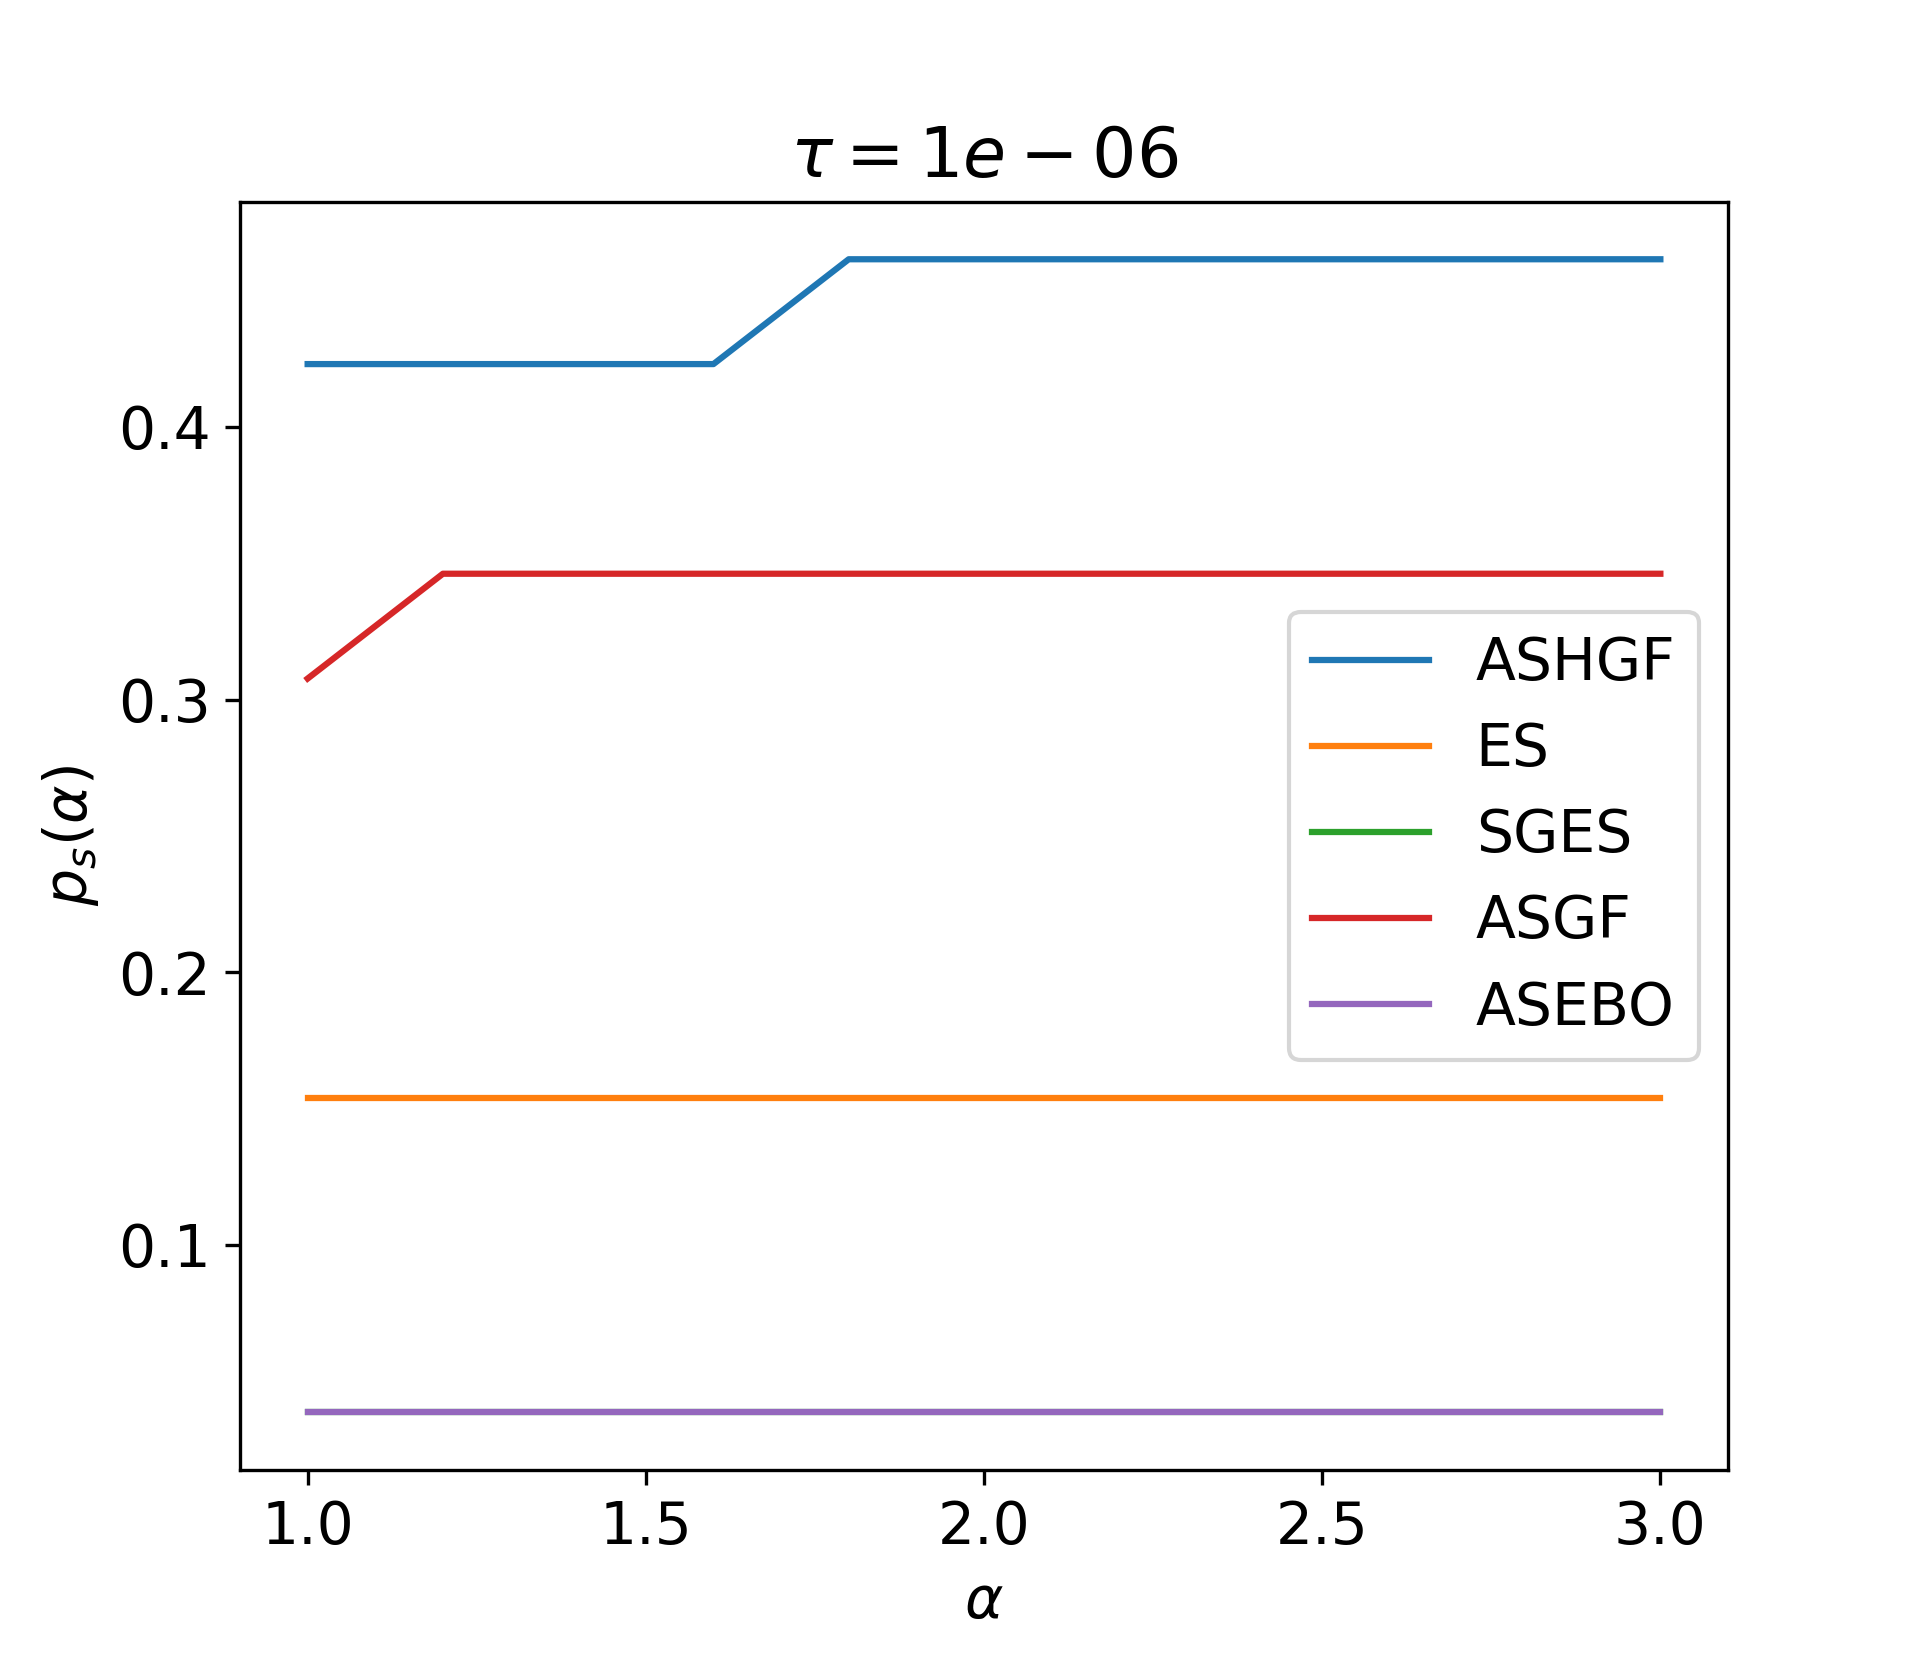
\includegraphics[width=1\textwidth]{figures/performance_profiles/1000/performance_profile_1000_1000000_1e-06.png}
\end{subfigure}
\centering
\begin{subfigure}{0.3\textwidth}
  \centering 
  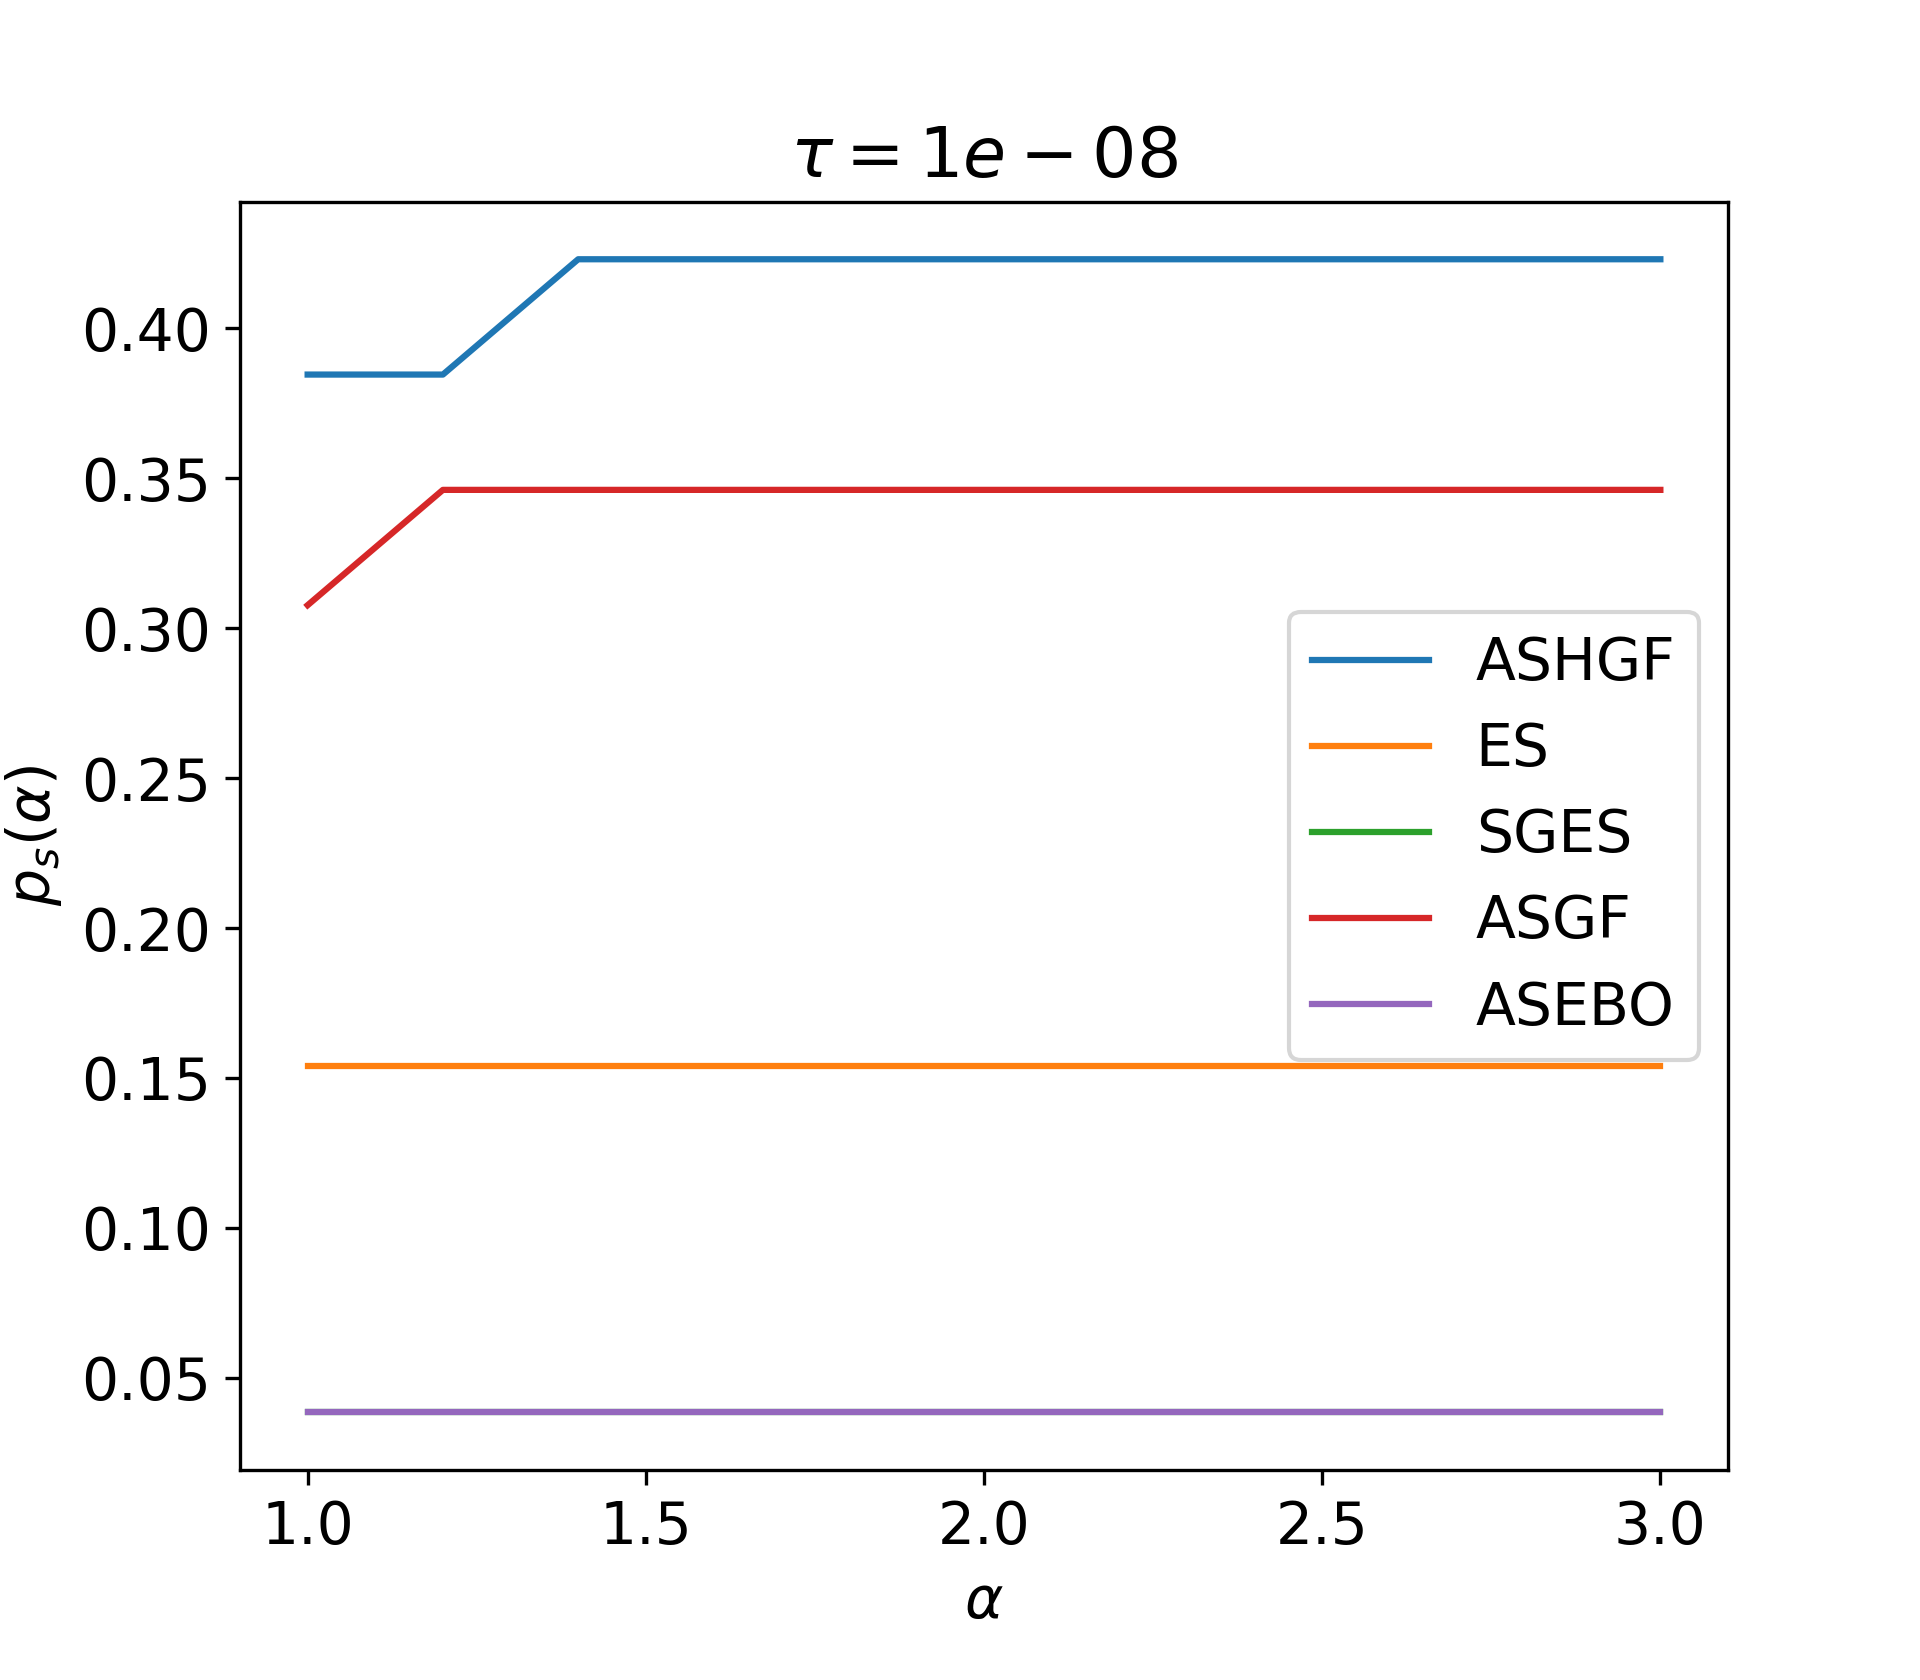
\includegraphics[width=1\textwidth]{figures/performance_profiles/1000/performance_profile_1000_1000000_1e-08.png}
\end{subfigure}%
\begin{subfigure}{0.3\textwidth}
  \centering 
  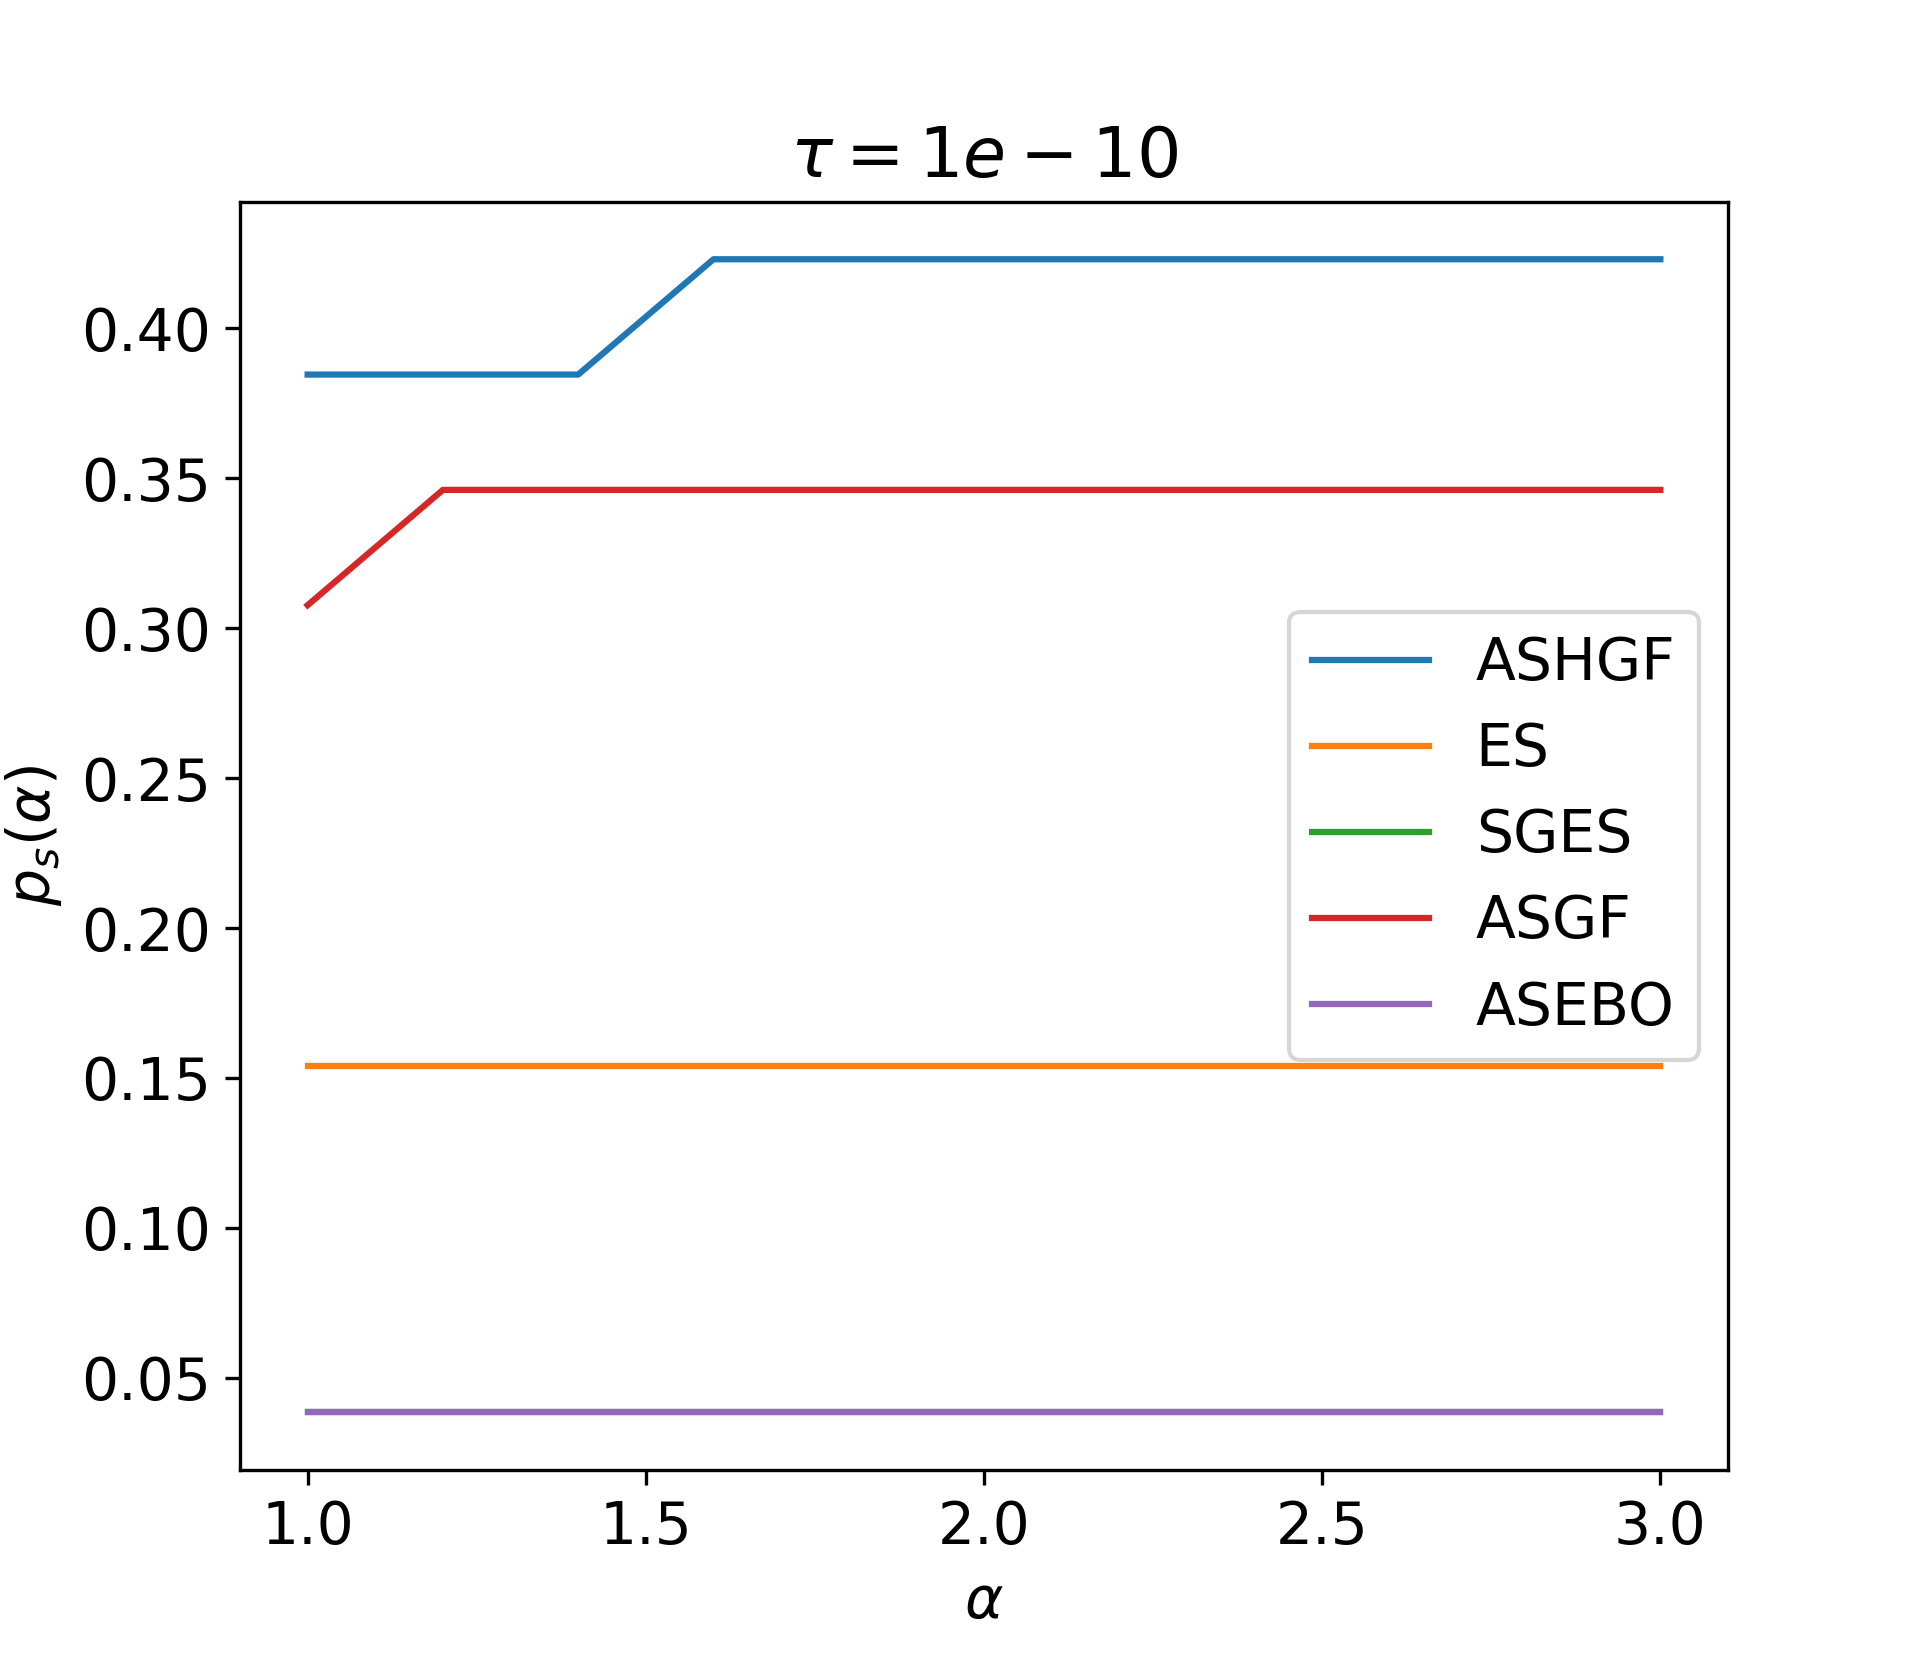
\includegraphics[width=1\textwidth]{figures/performance_profiles/1000/performance_profile_1000_1000000_1e-10.png}
\end{subfigure}
\caption{Performance profiles with $\mu_L = 10^{6}$}
\label{PerformanceProfiles1000Mu1000000}
\end{figure}

\begin{figure}[H]
\centering
\begin{subfigure}{0.3\textwidth}
  \centering 
  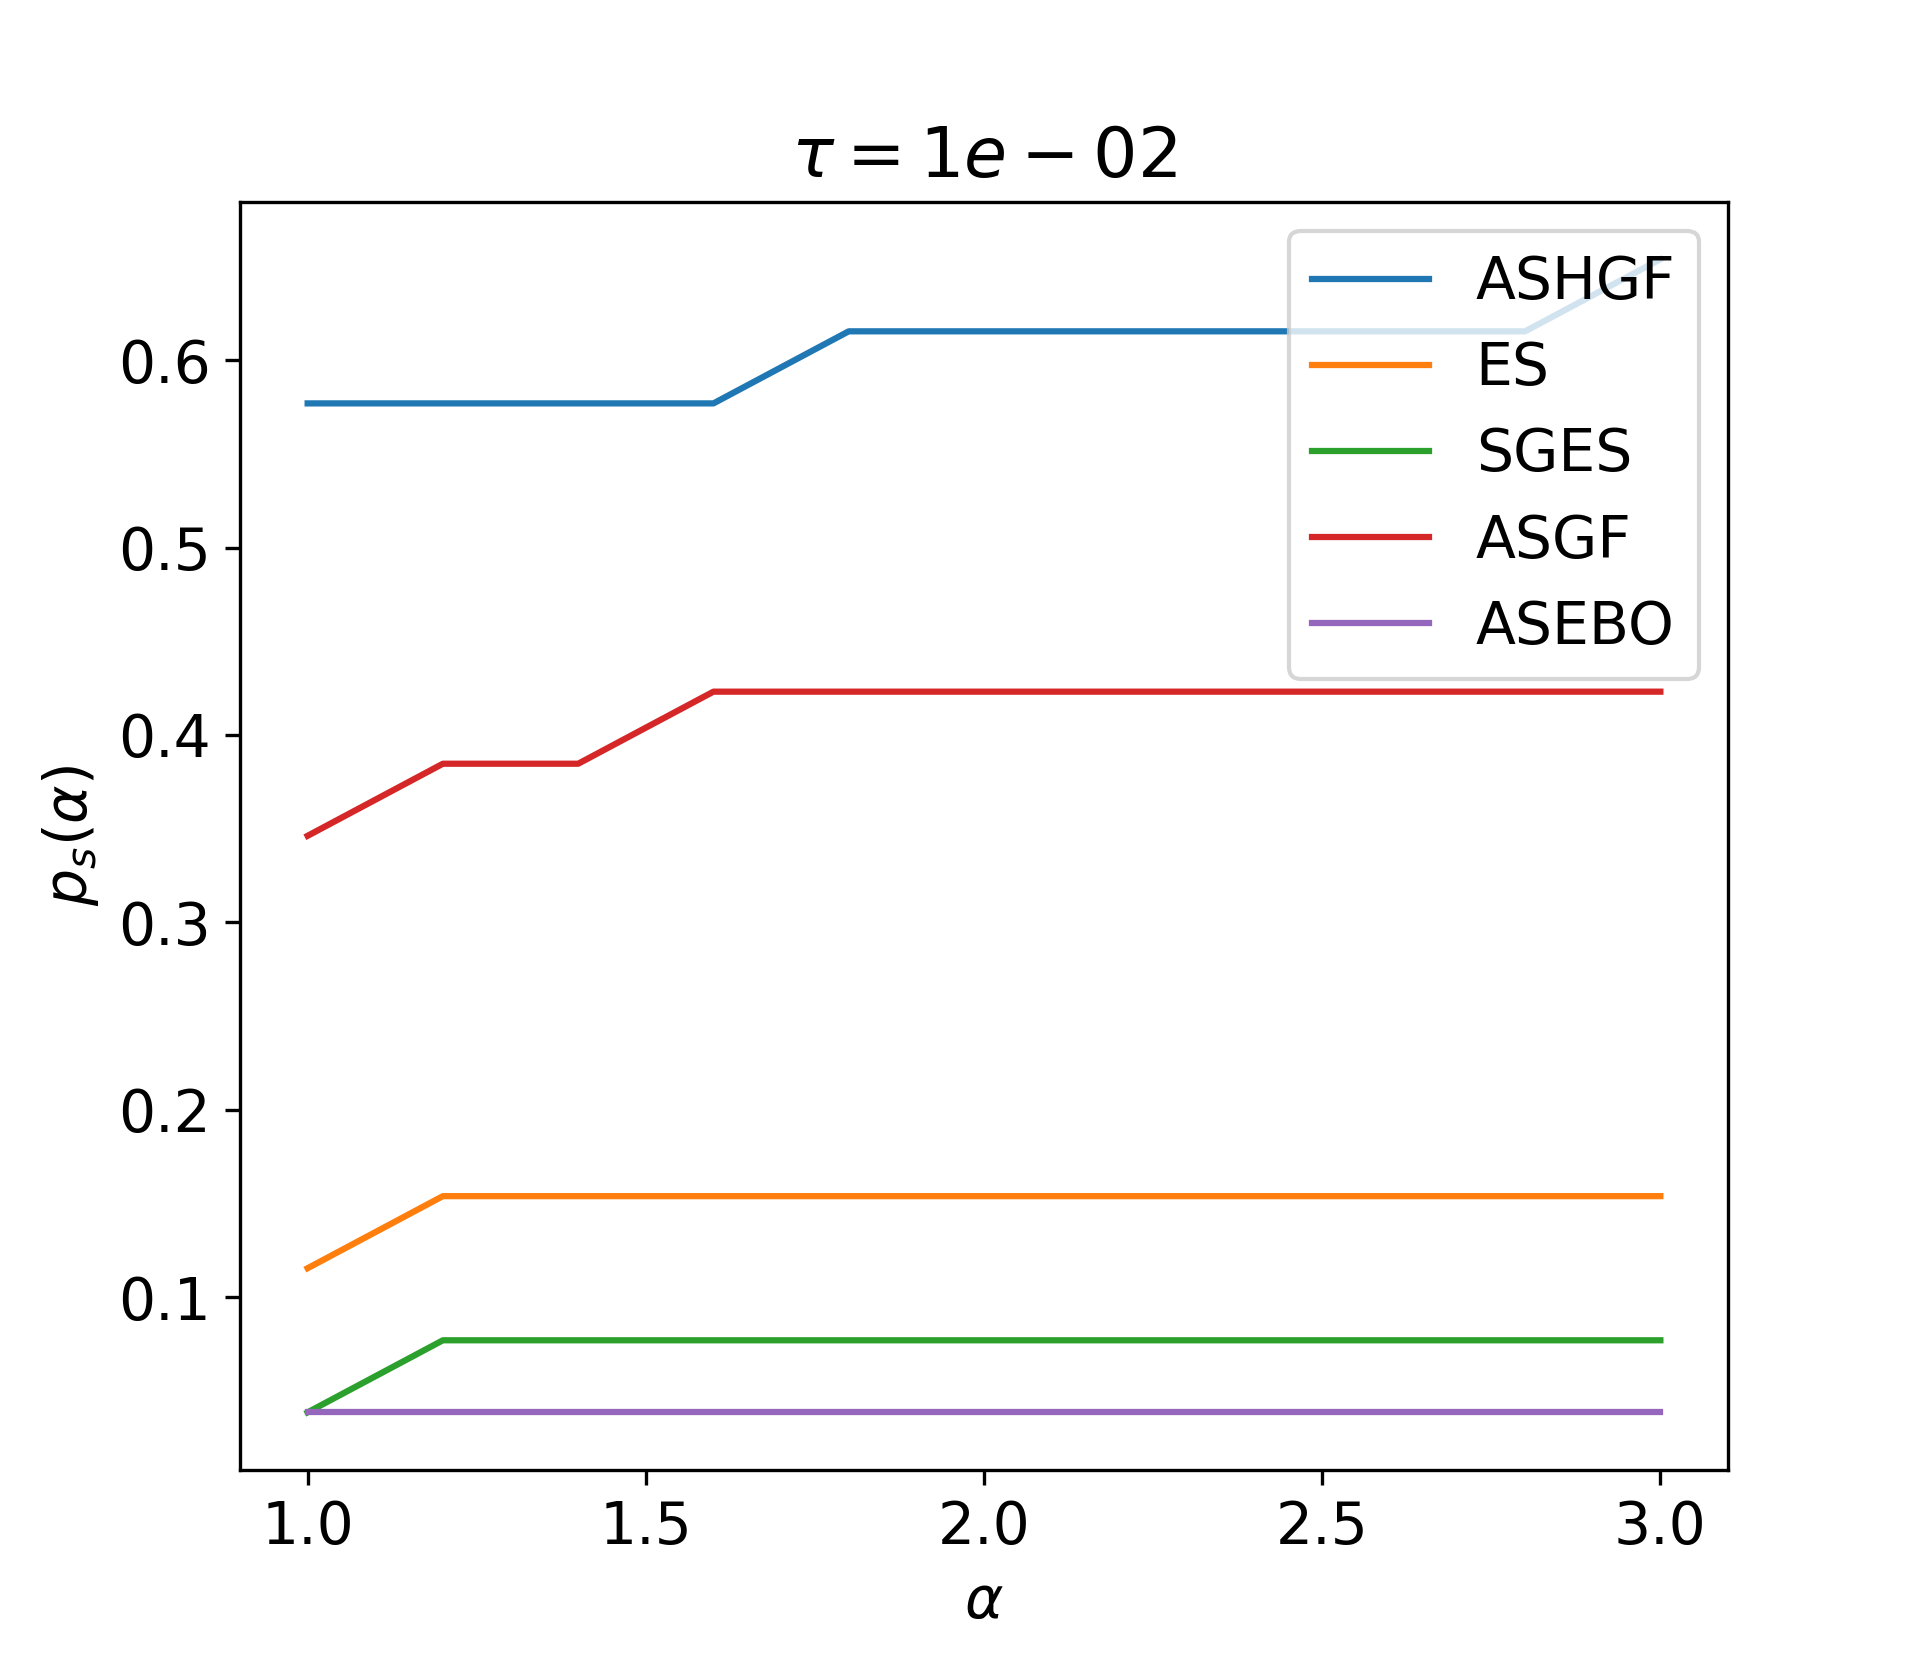
\includegraphics[width=1\textwidth]{figures/performance_profiles/1000/performance_profile_1000_10000000_1e-02.png}
\end{subfigure}%
\begin{subfigure}{0.3\textwidth}
  \centering 
  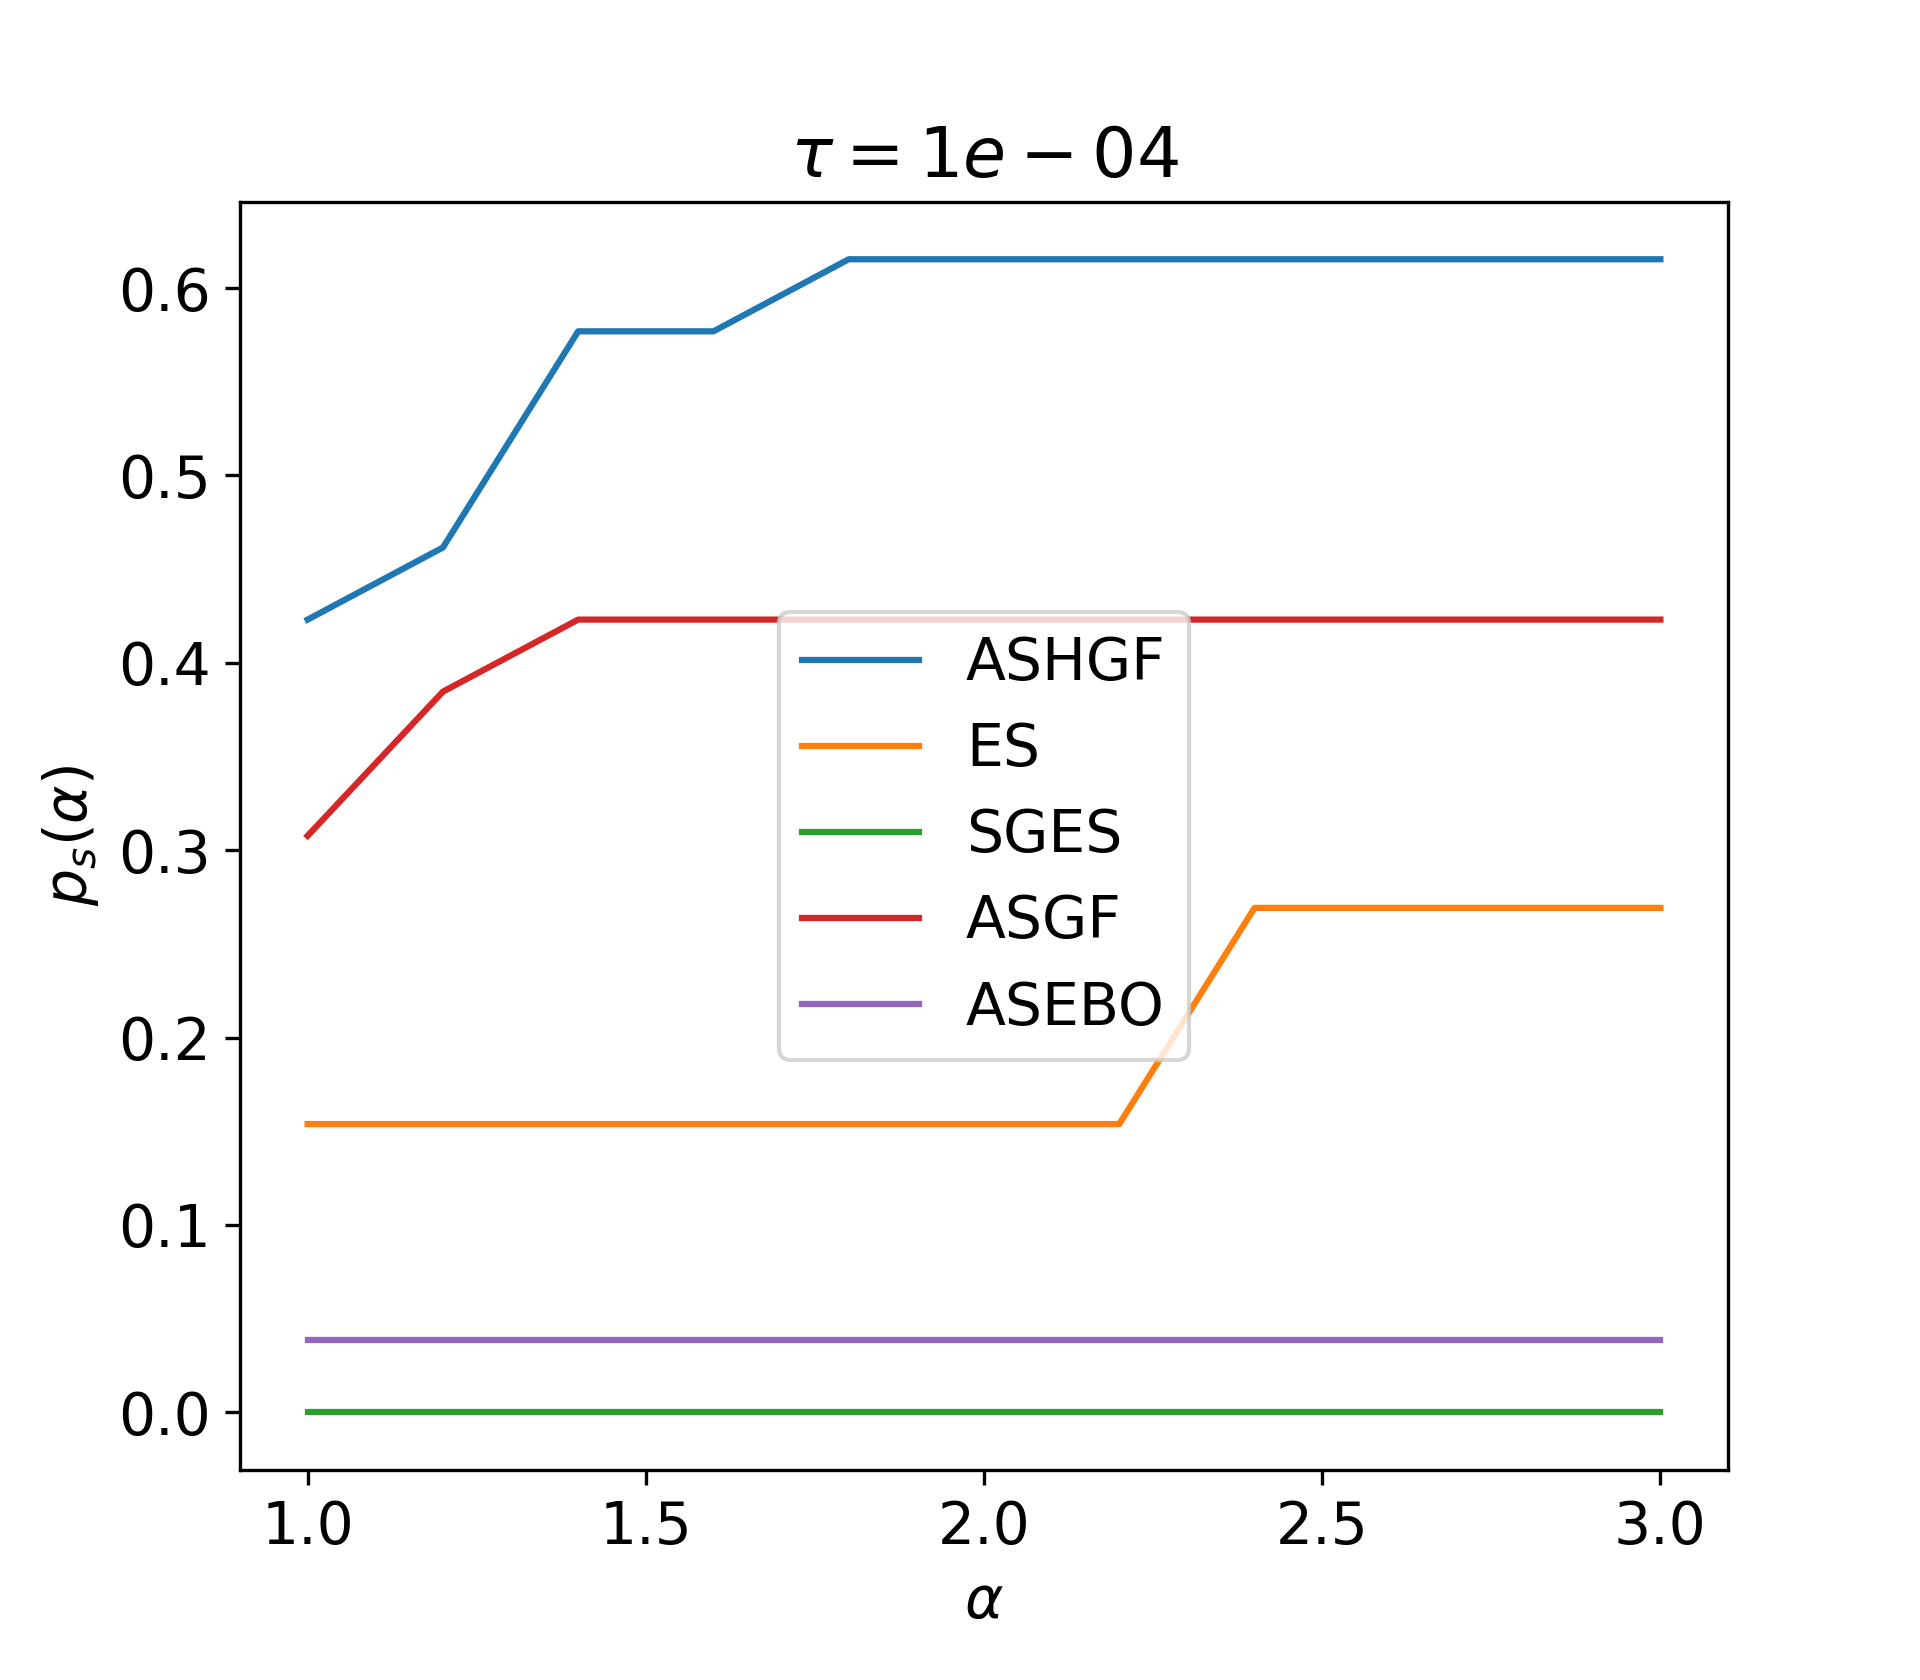
\includegraphics[width=1\textwidth]{figures/performance_profiles/1000/performance_profile_1000_10000000_1e-04.png}
\end{subfigure}
\begin{subfigure}{0.3\textwidth}
  \centering 
  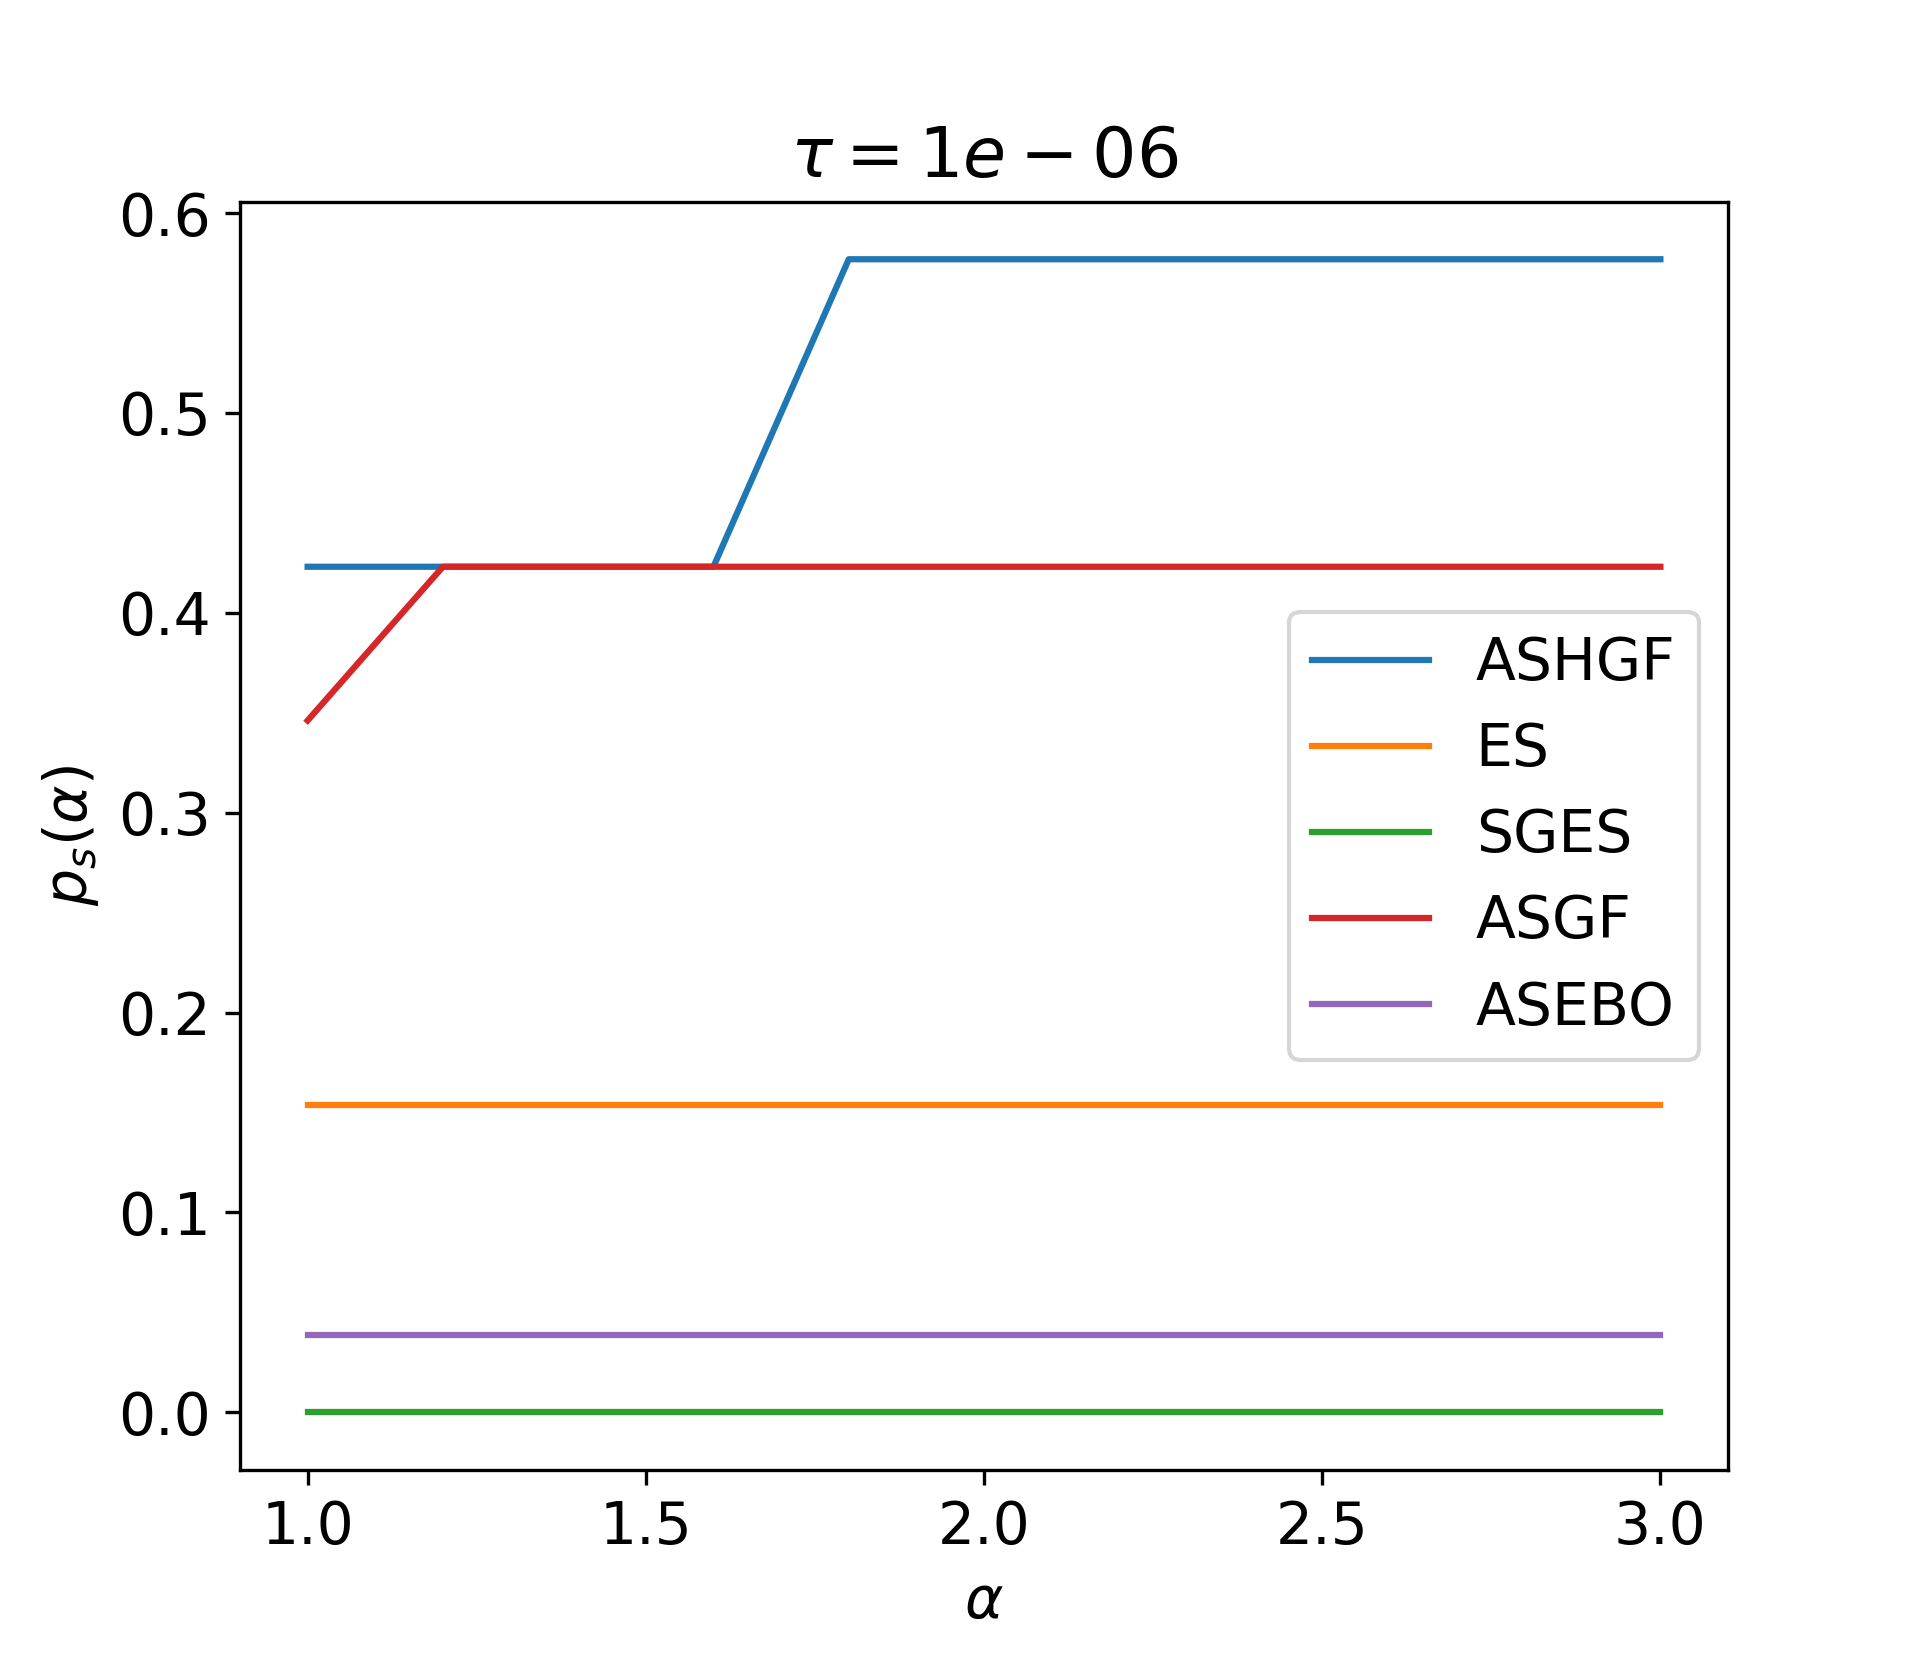
\includegraphics[width=1\textwidth]{figures/performance_profiles/1000/performance_profile_1000_10000000_1e-06.png}
\end{subfigure}
\centering
\begin{subfigure}{0.3\textwidth}
  \centering 
  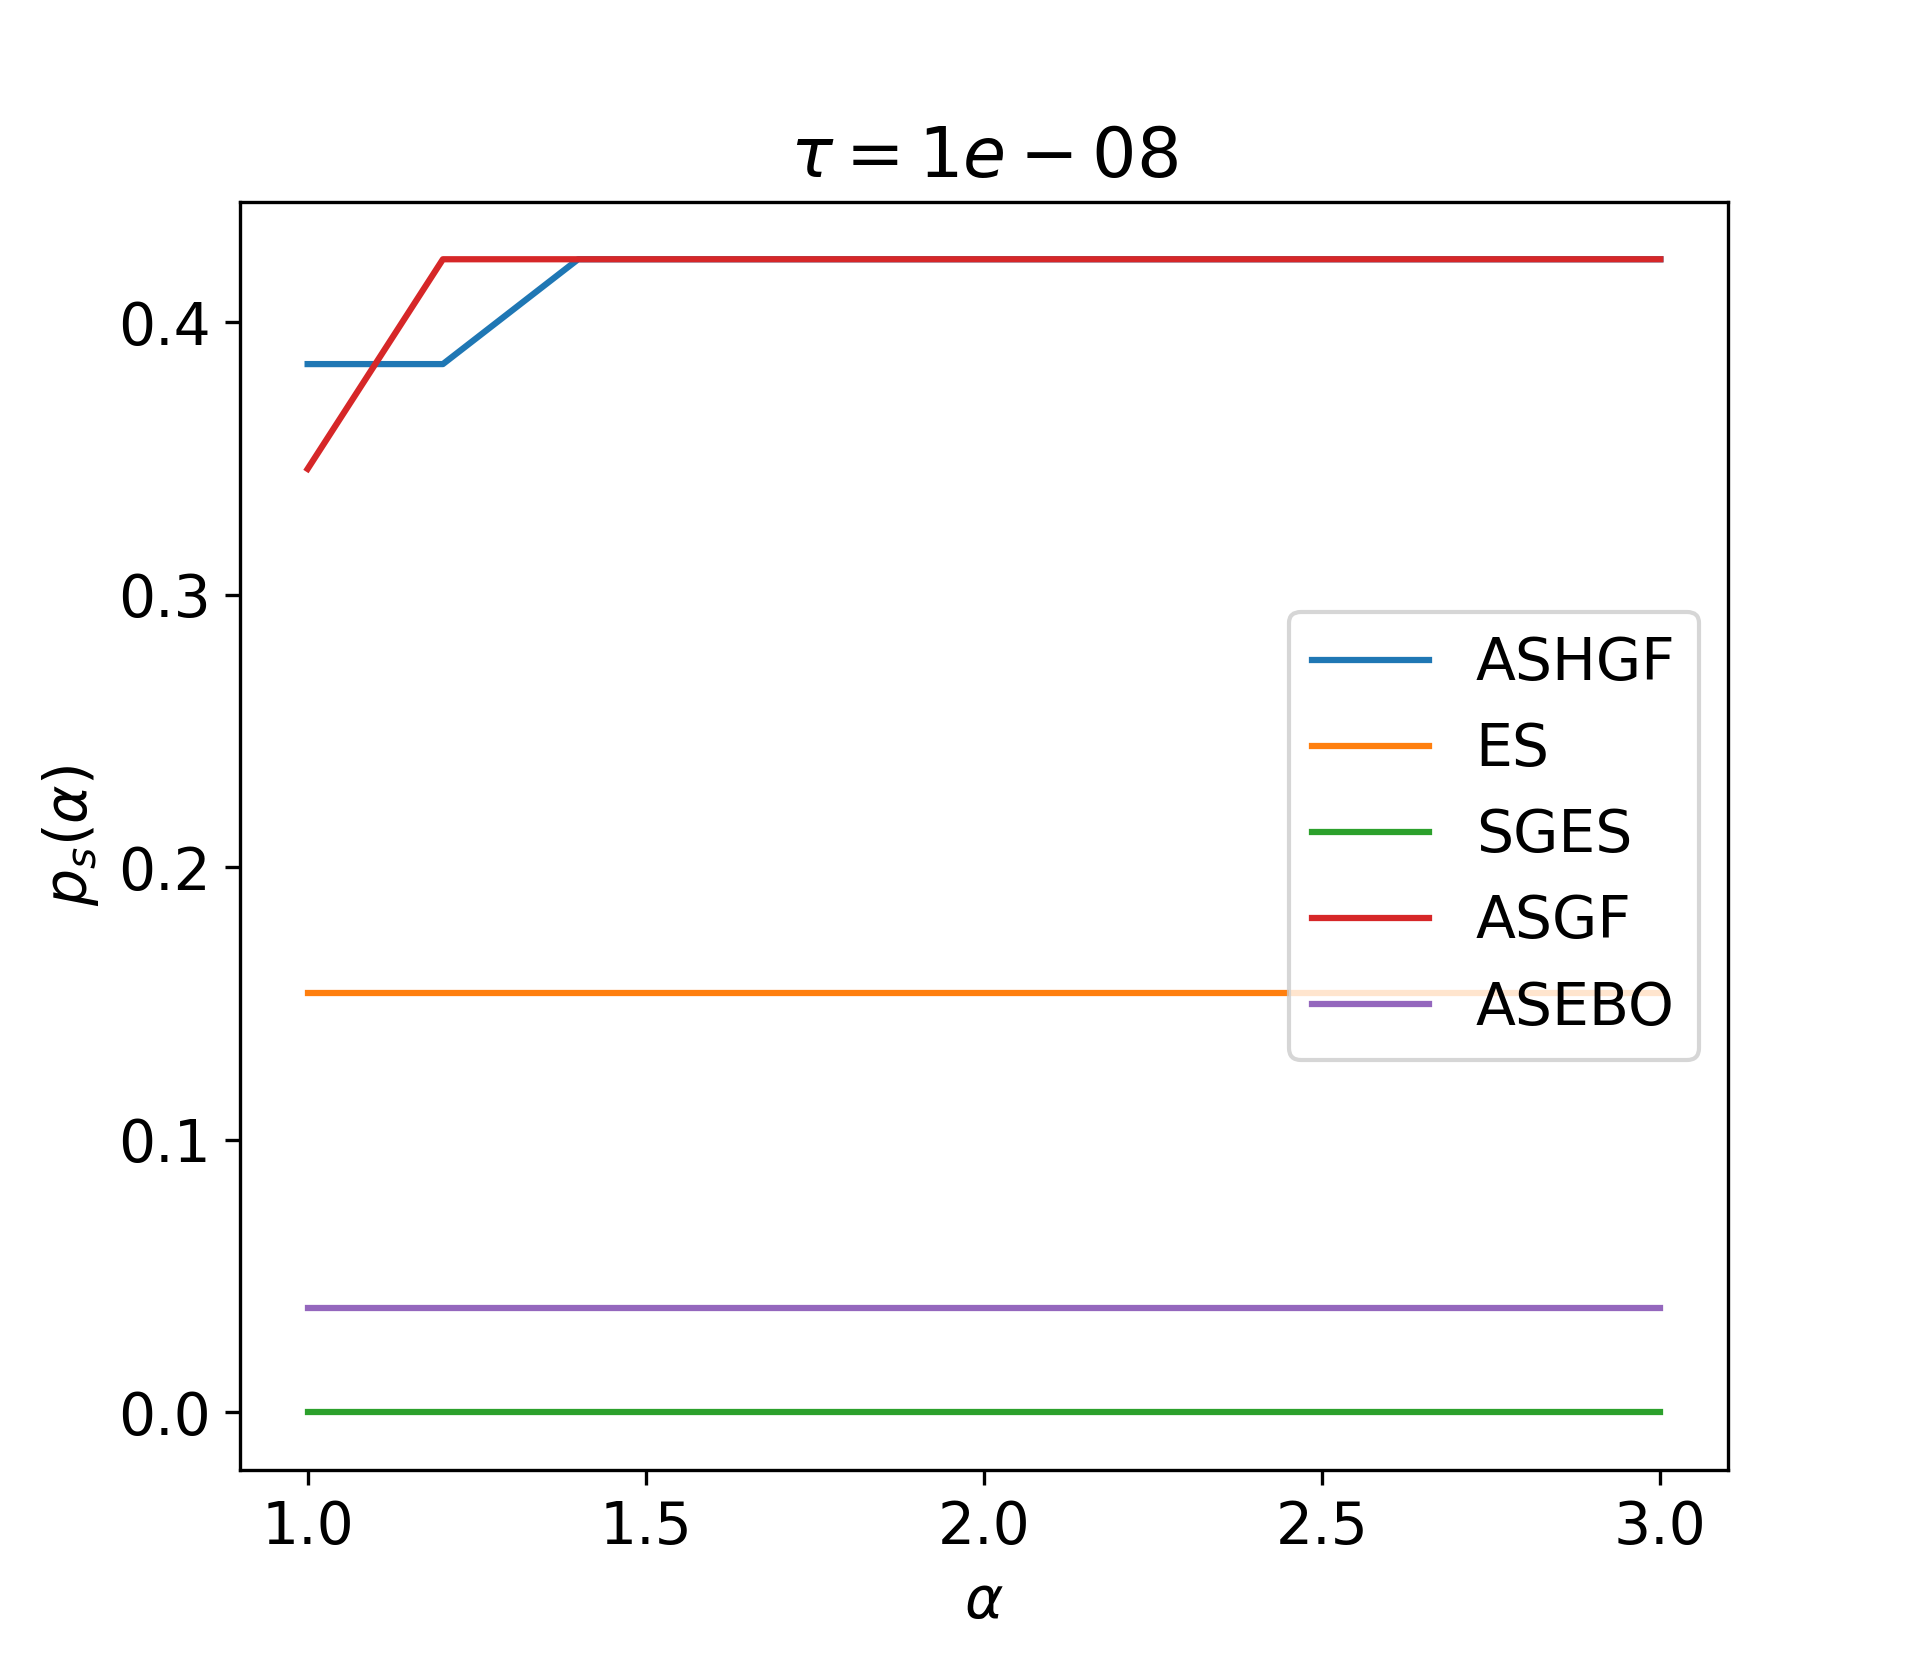
\includegraphics[width=1\textwidth]{figures/performance_profiles/1000/performance_profile_1000_10000000_1e-08.png}
\end{subfigure}%
\begin{subfigure}{0.3\textwidth}
  \centering 
  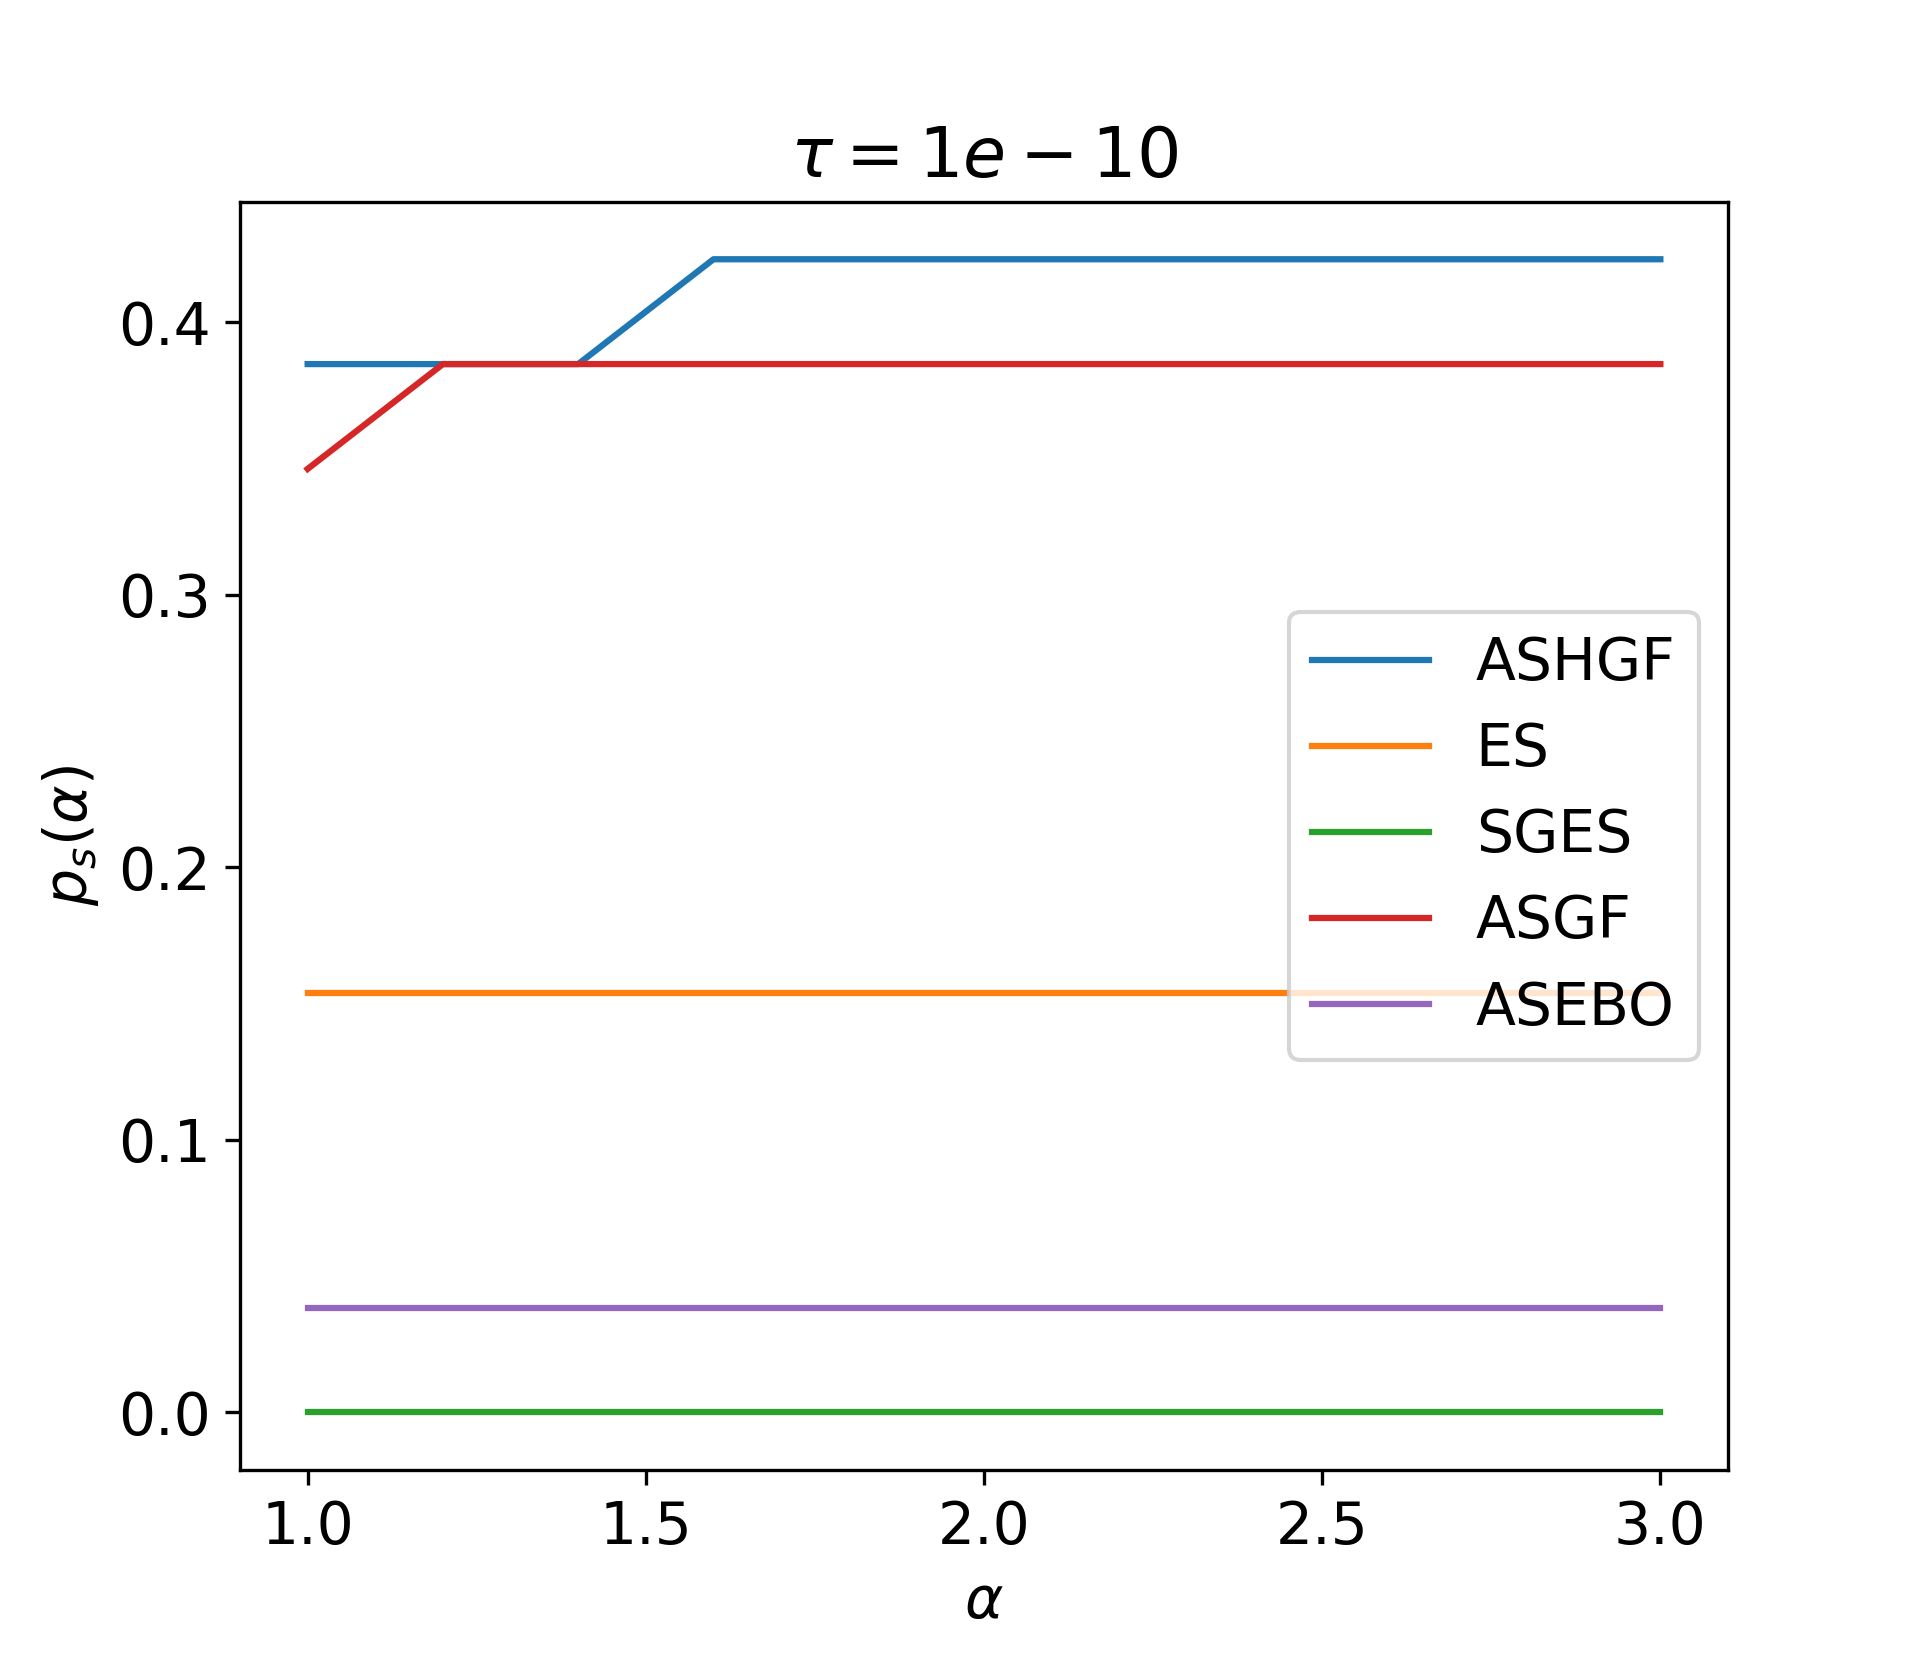
\includegraphics[width=1\textwidth]{figures/performance_profiles/1000/performance_profile_1000_10000000_1e-10.png}
\end{subfigure}
\caption{Performance profiles with $\mu_L = 10^{7}$}
\label{PerformanceProfiles1000Mu10000000}
\end{figure}

\begin{figure}[H]
	\centering
	\begin{subfigure}{0.3\textwidth}
		\centering 
		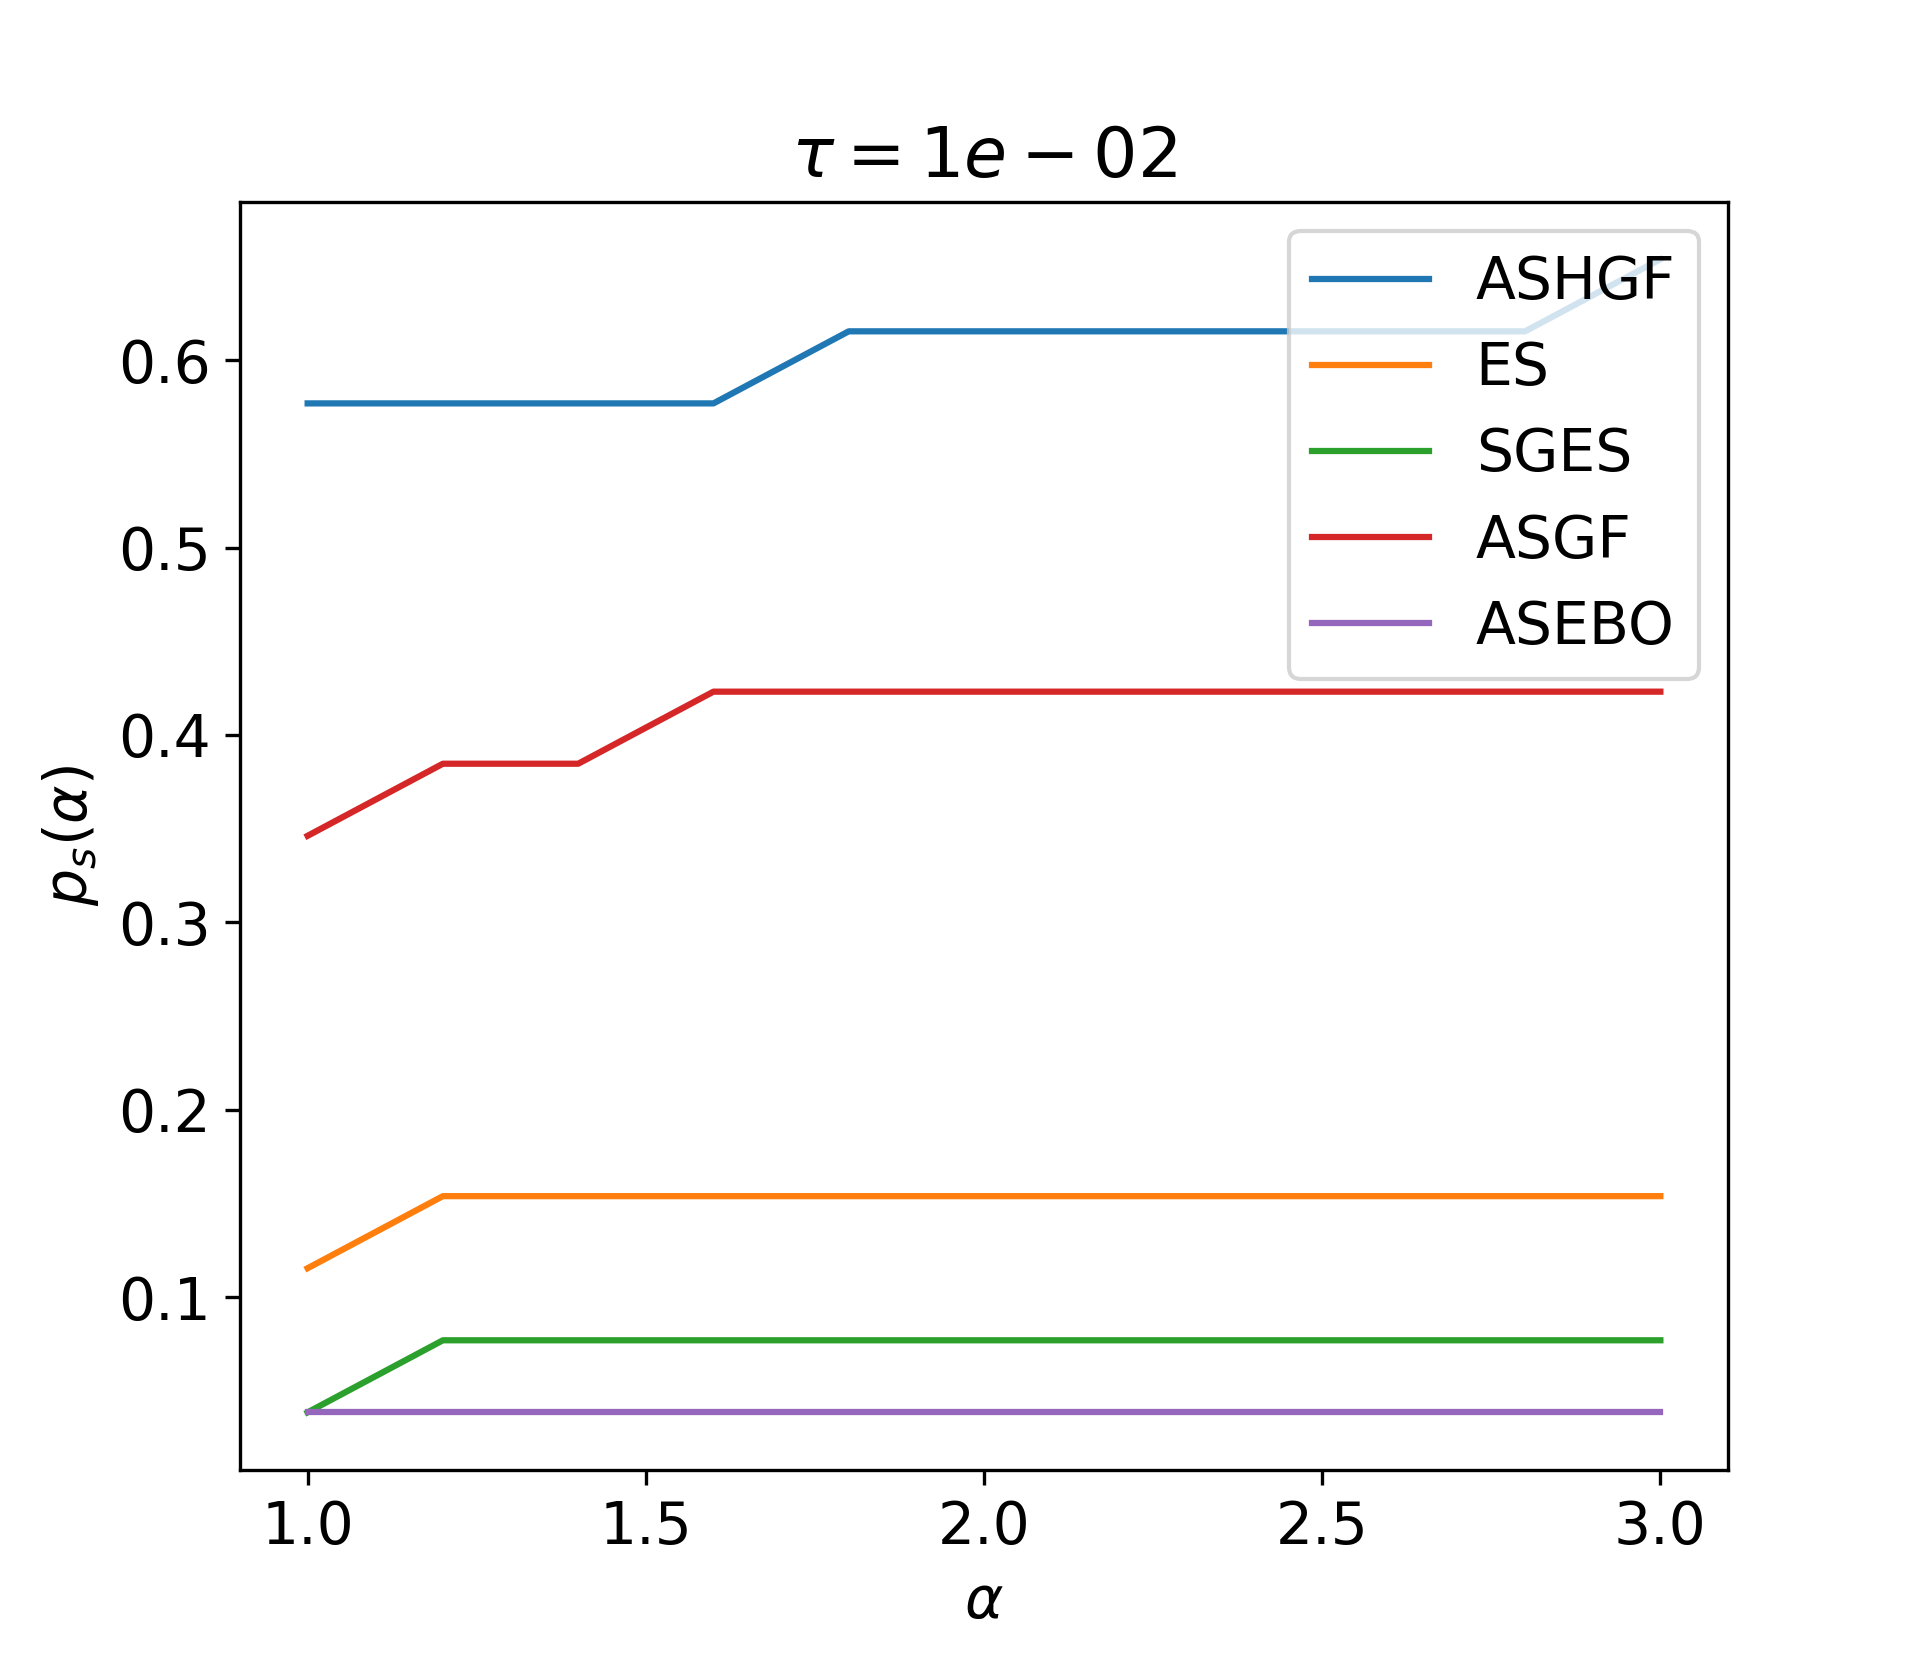
\includegraphics[width=1\textwidth]{figures/performance_profiles/1000/performance_profile_1000_100000000_1e-02.png}
	\end{subfigure}%
	\begin{subfigure}{0.3\textwidth}
		\centering 
		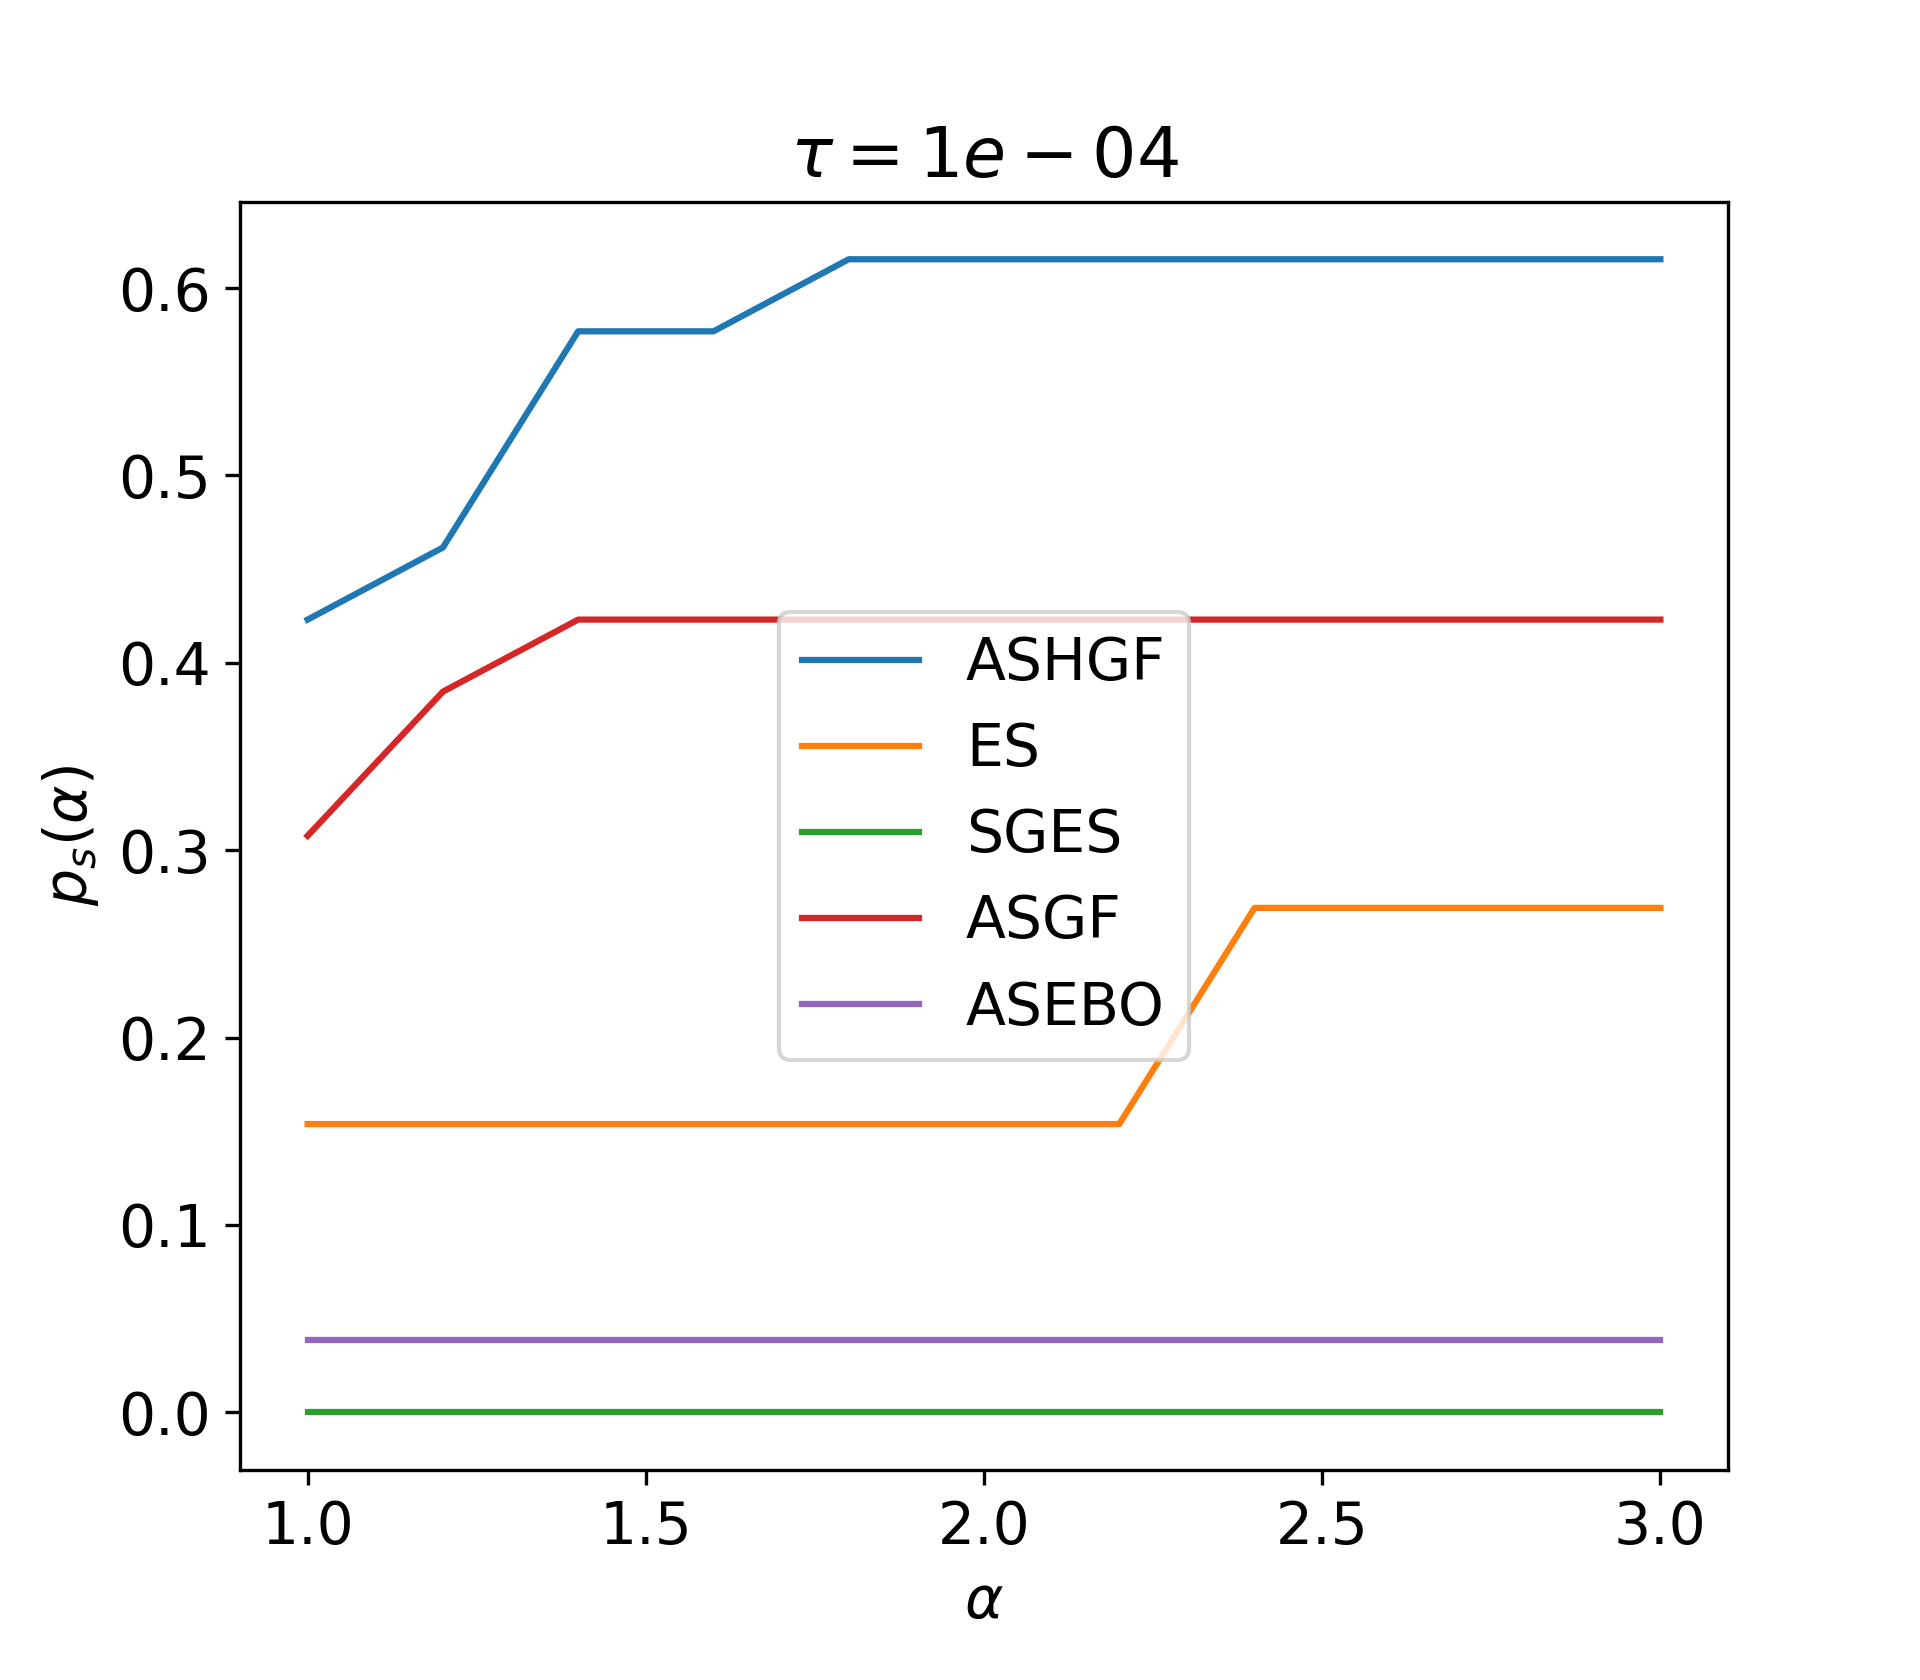
\includegraphics[width=1\textwidth]{figures/performance_profiles/1000/performance_profile_1000_100000000_1e-04.png}
	\end{subfigure}
	\begin{subfigure}{0.3\textwidth}
		\centering 
		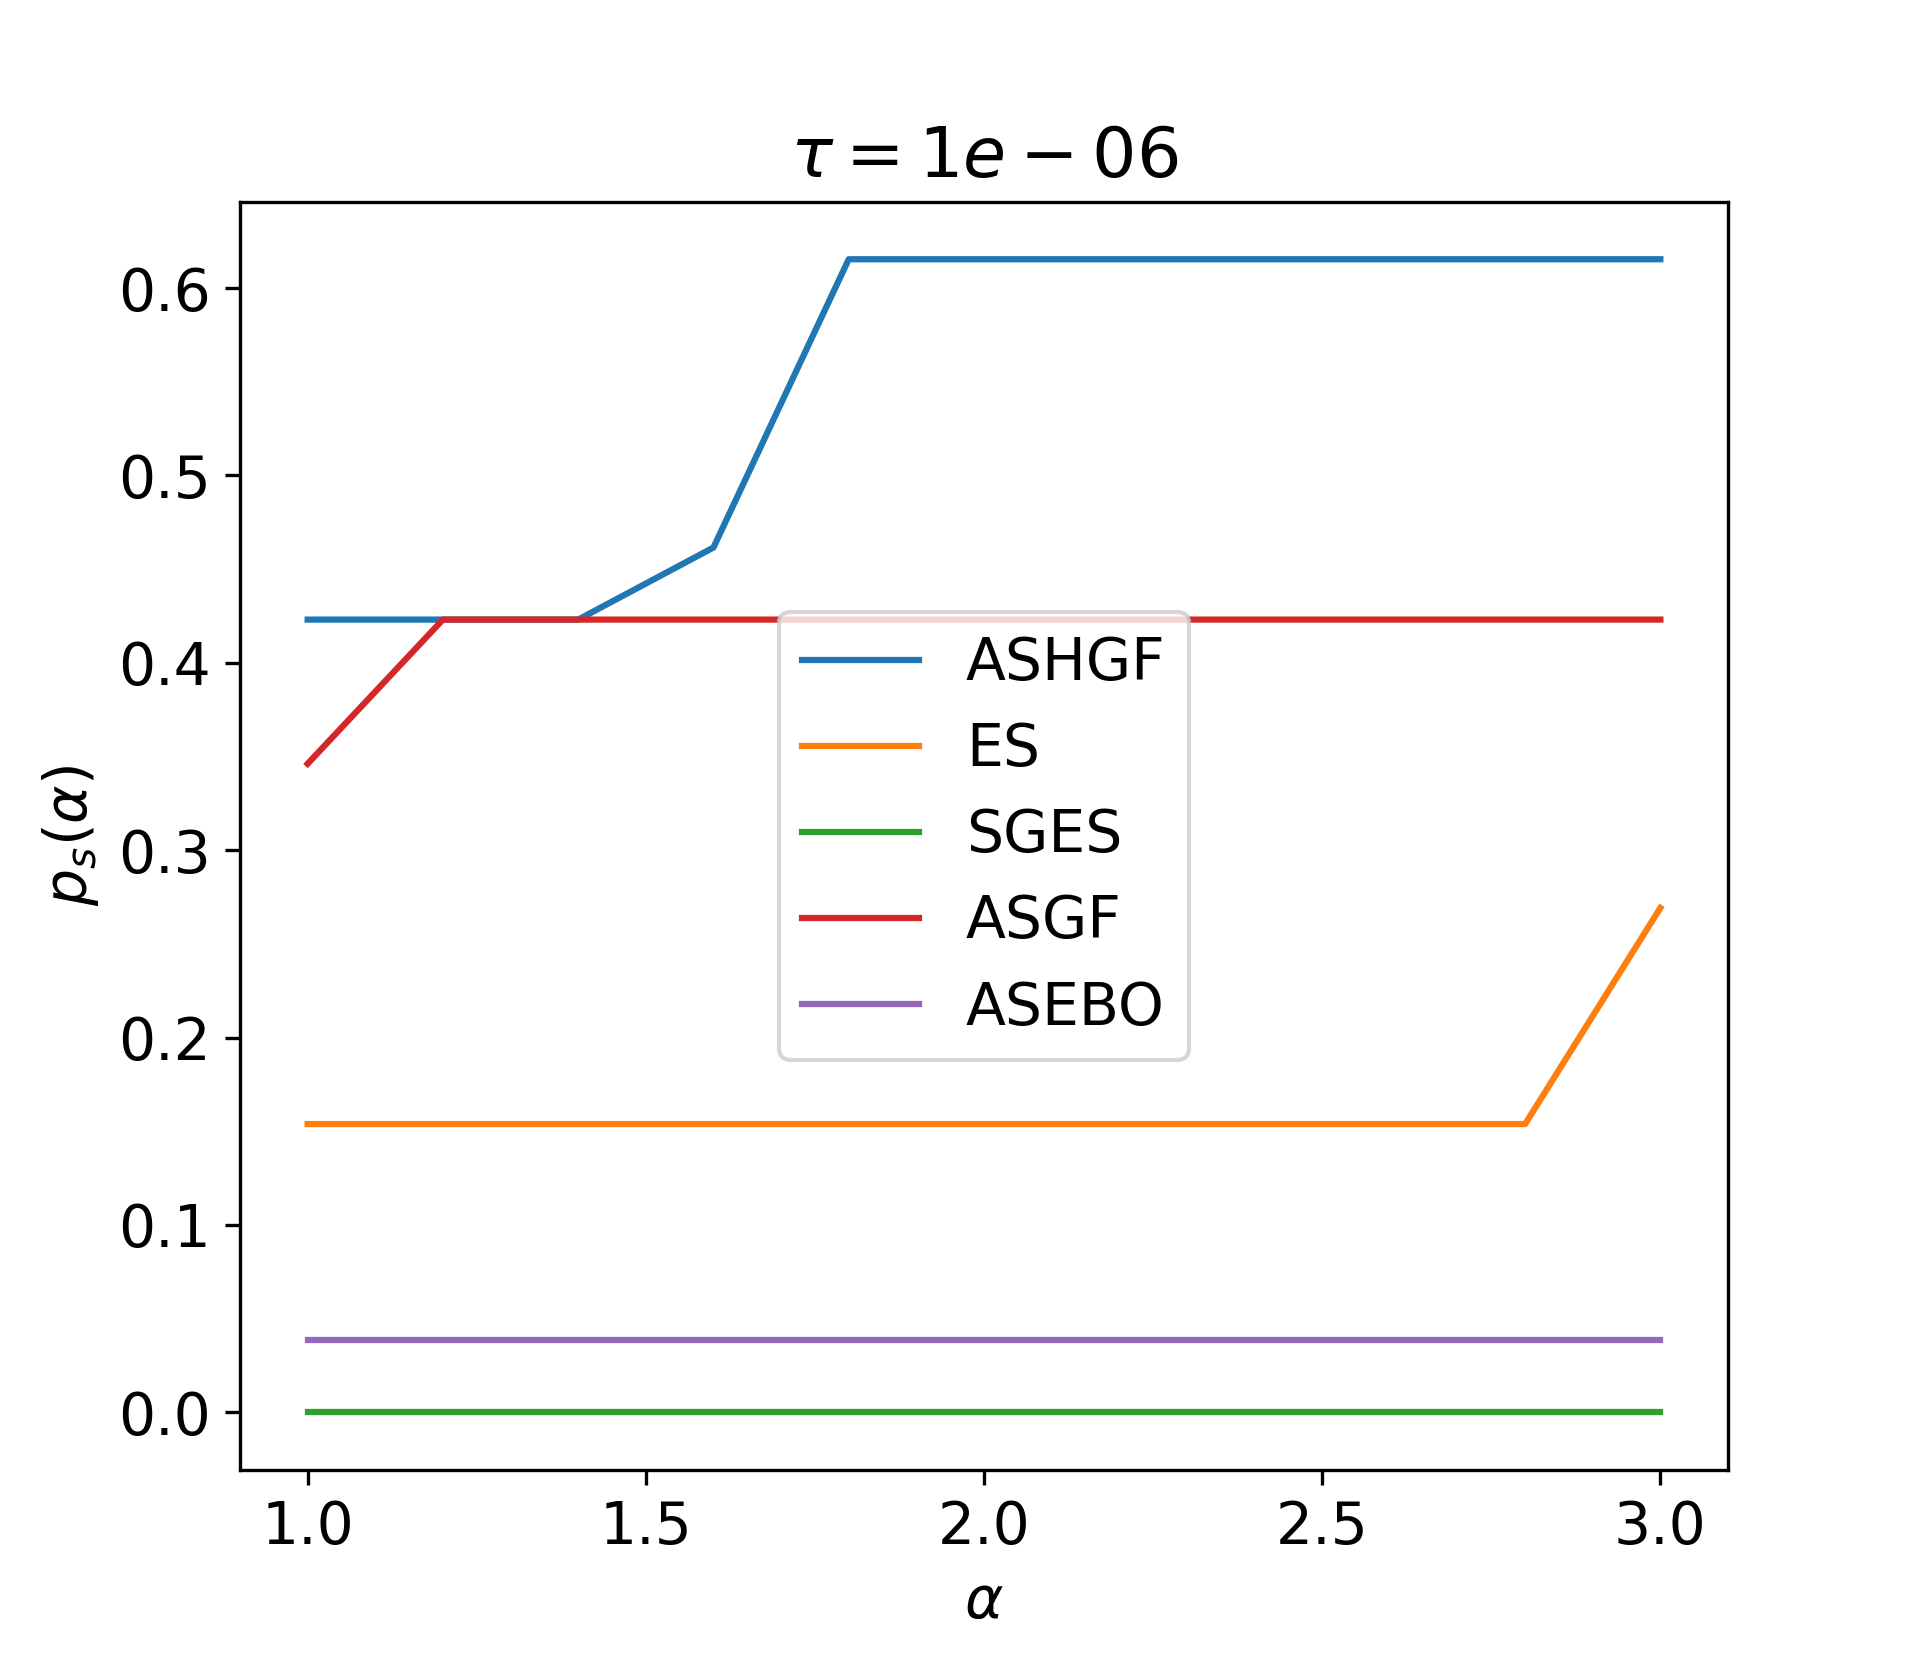
\includegraphics[width=1\textwidth]{figures/performance_profiles/1000/performance_profile_1000_100000000_1e-06.png}
	\end{subfigure}
	\centering
	\begin{subfigure}{0.3\textwidth}
		\centering 
		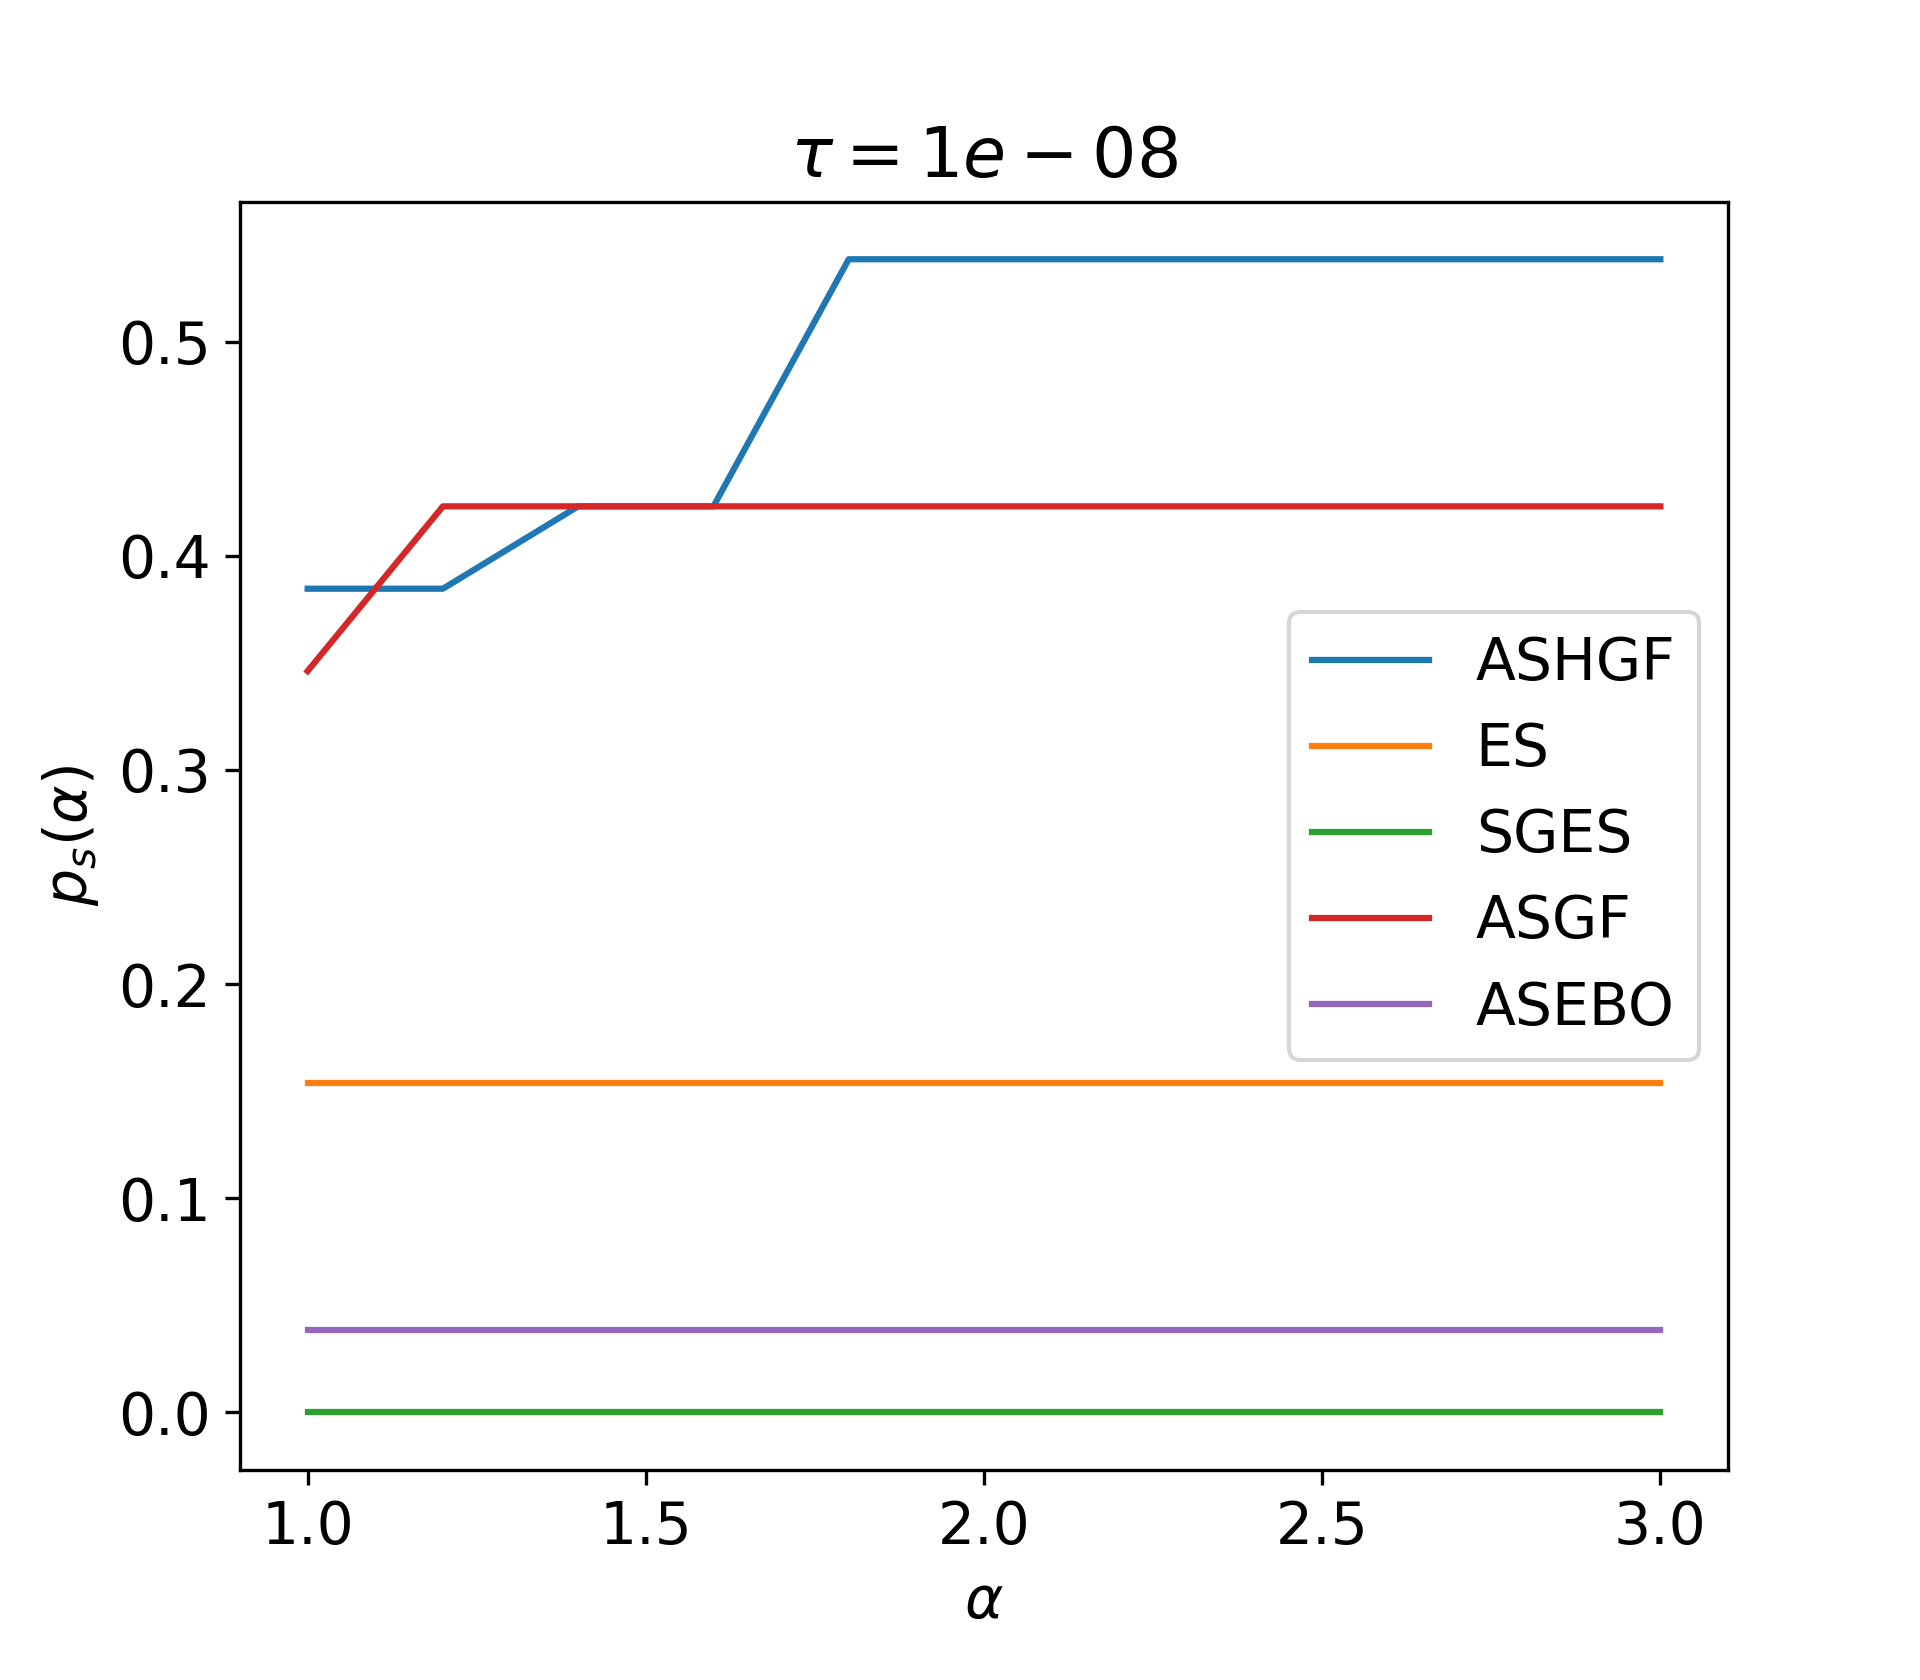
\includegraphics[width=1\textwidth]{figures/performance_profiles/1000/performance_profile_1000_100000000_1e-08.png}
	\end{subfigure}%
	\begin{subfigure}{0.3\textwidth}
		\centering 
		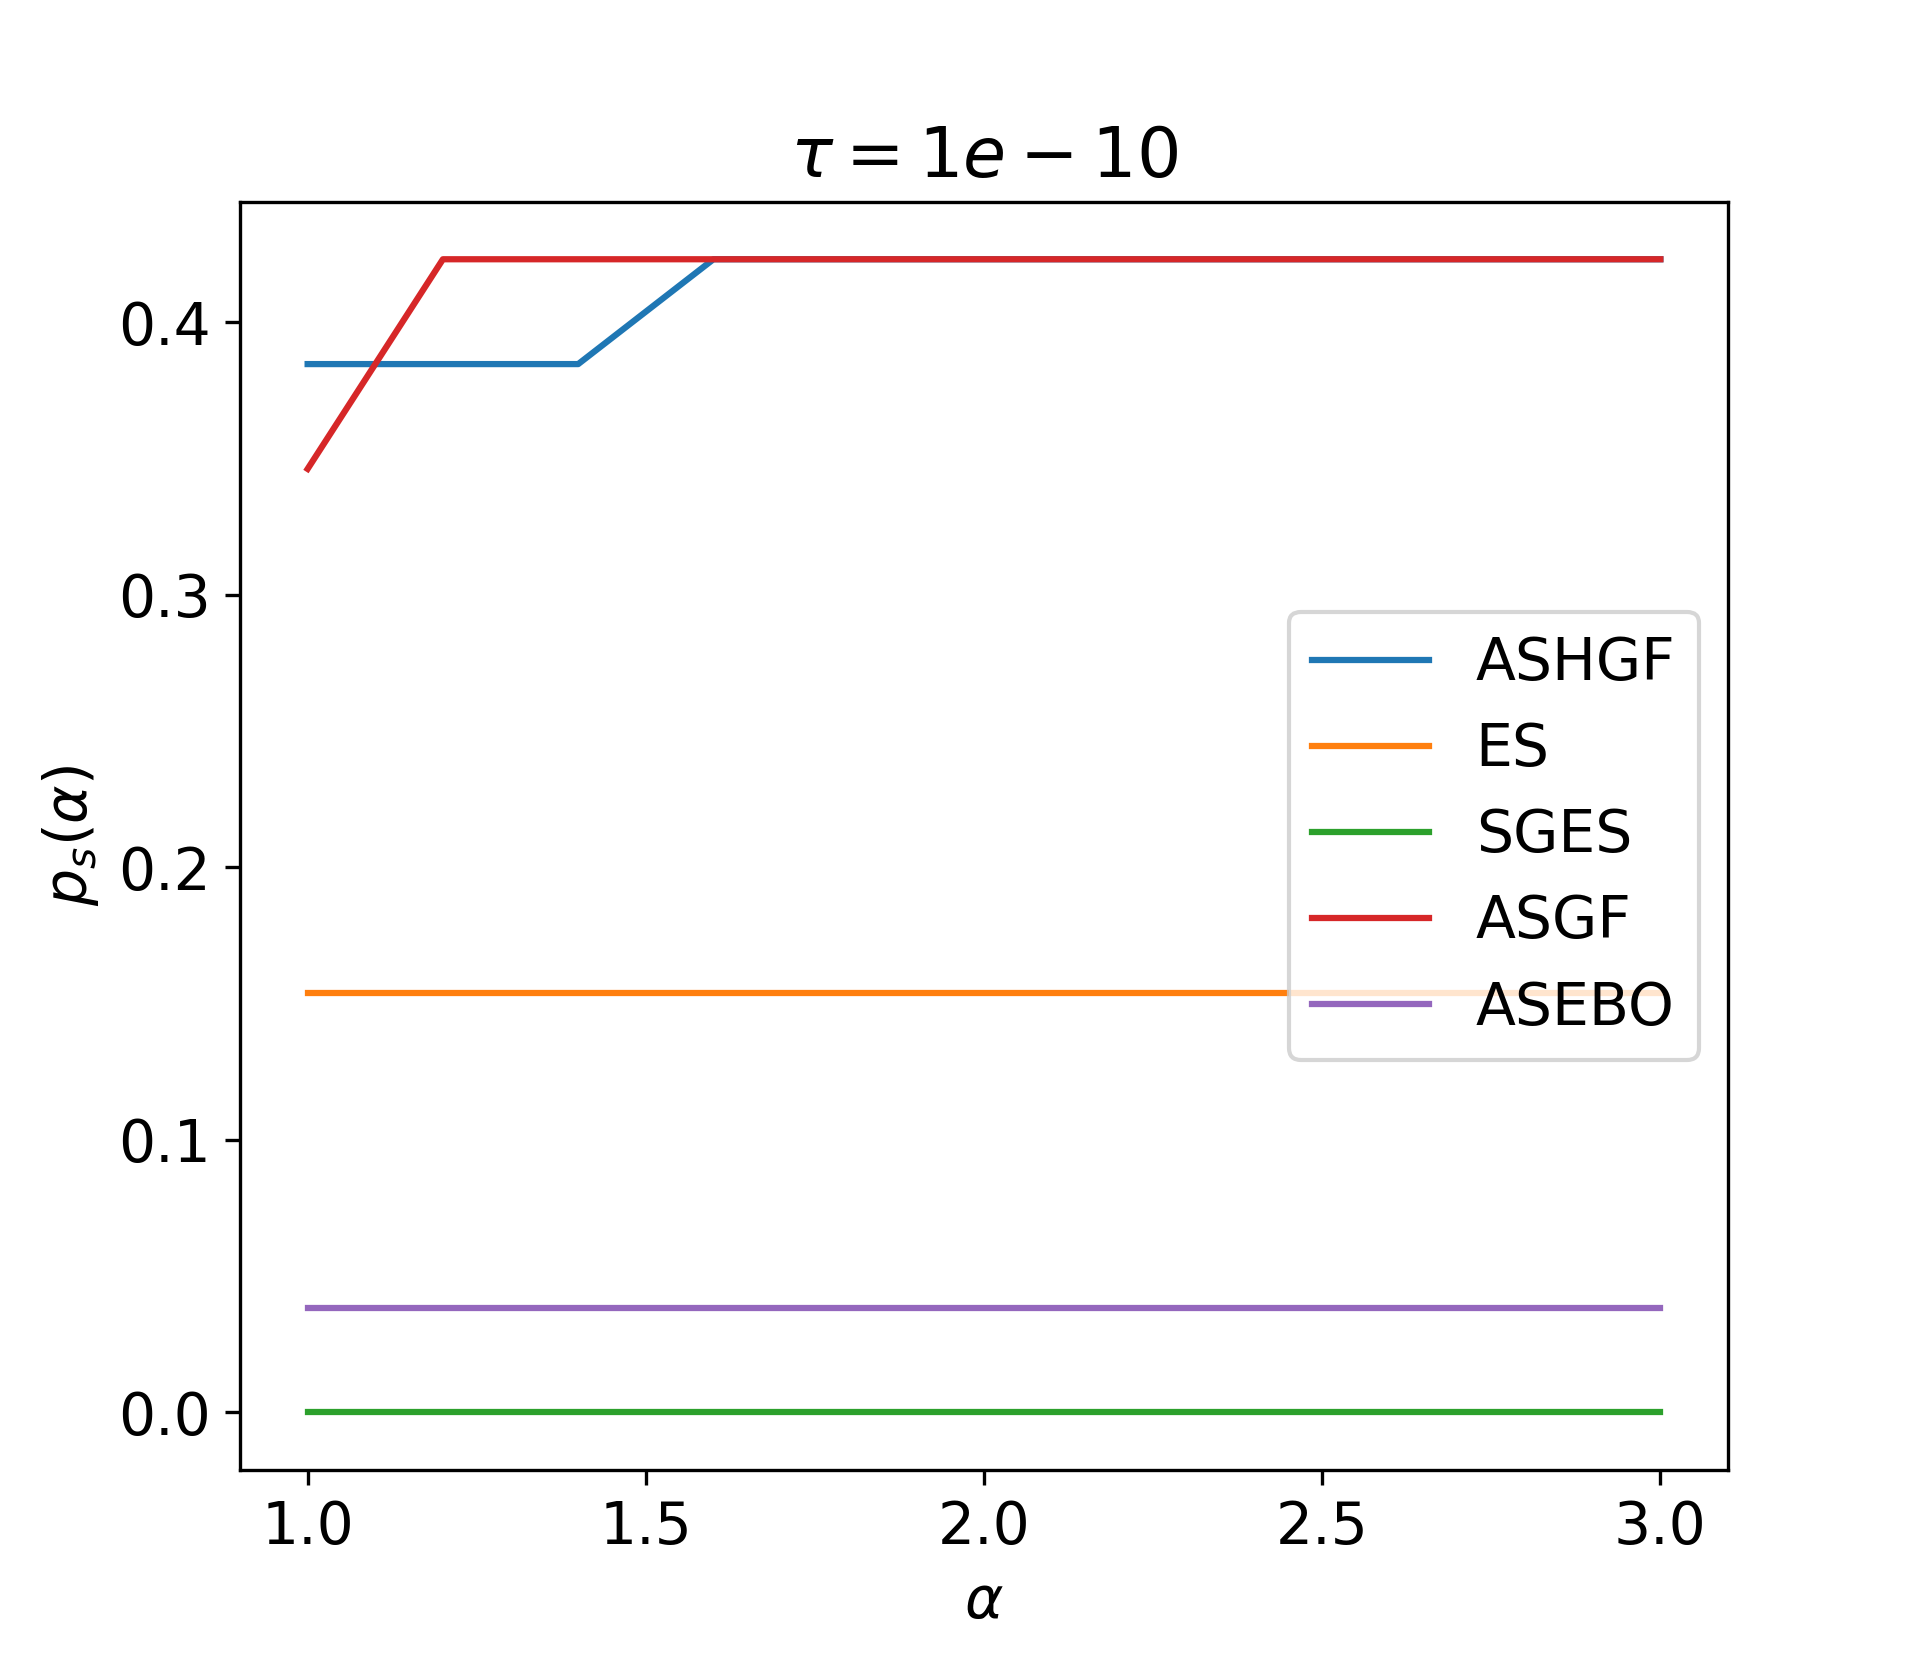
\includegraphics[width=1\textwidth]{figures/performance_profiles/1000/performance_profile_1000_100000000_1e-10.png}
	\end{subfigure}
	\caption{Performance profiles with $\mu_L = 10^{8}$}
	\label{PerformanceProfiles1000Mu100000000}
\end{figure}

\subsection{Data profiles}

With this quantity is measured the percentage of problems solved within a tolerance $\tau$ for a certain number of function evaluations.

As it can be seen with the performance profiles, again thanks to the data profiles it can be seen that increasing the dimensionality of the problem, ASHGF requires increased budget. Given that, the algorithm shows itself to be more efficient than others given a bigger budget.

\subsubsection{Dimension 10}

\begin{figure}[H]
\centering
\begin{subfigure}{0.3\textwidth}
  \centering 
  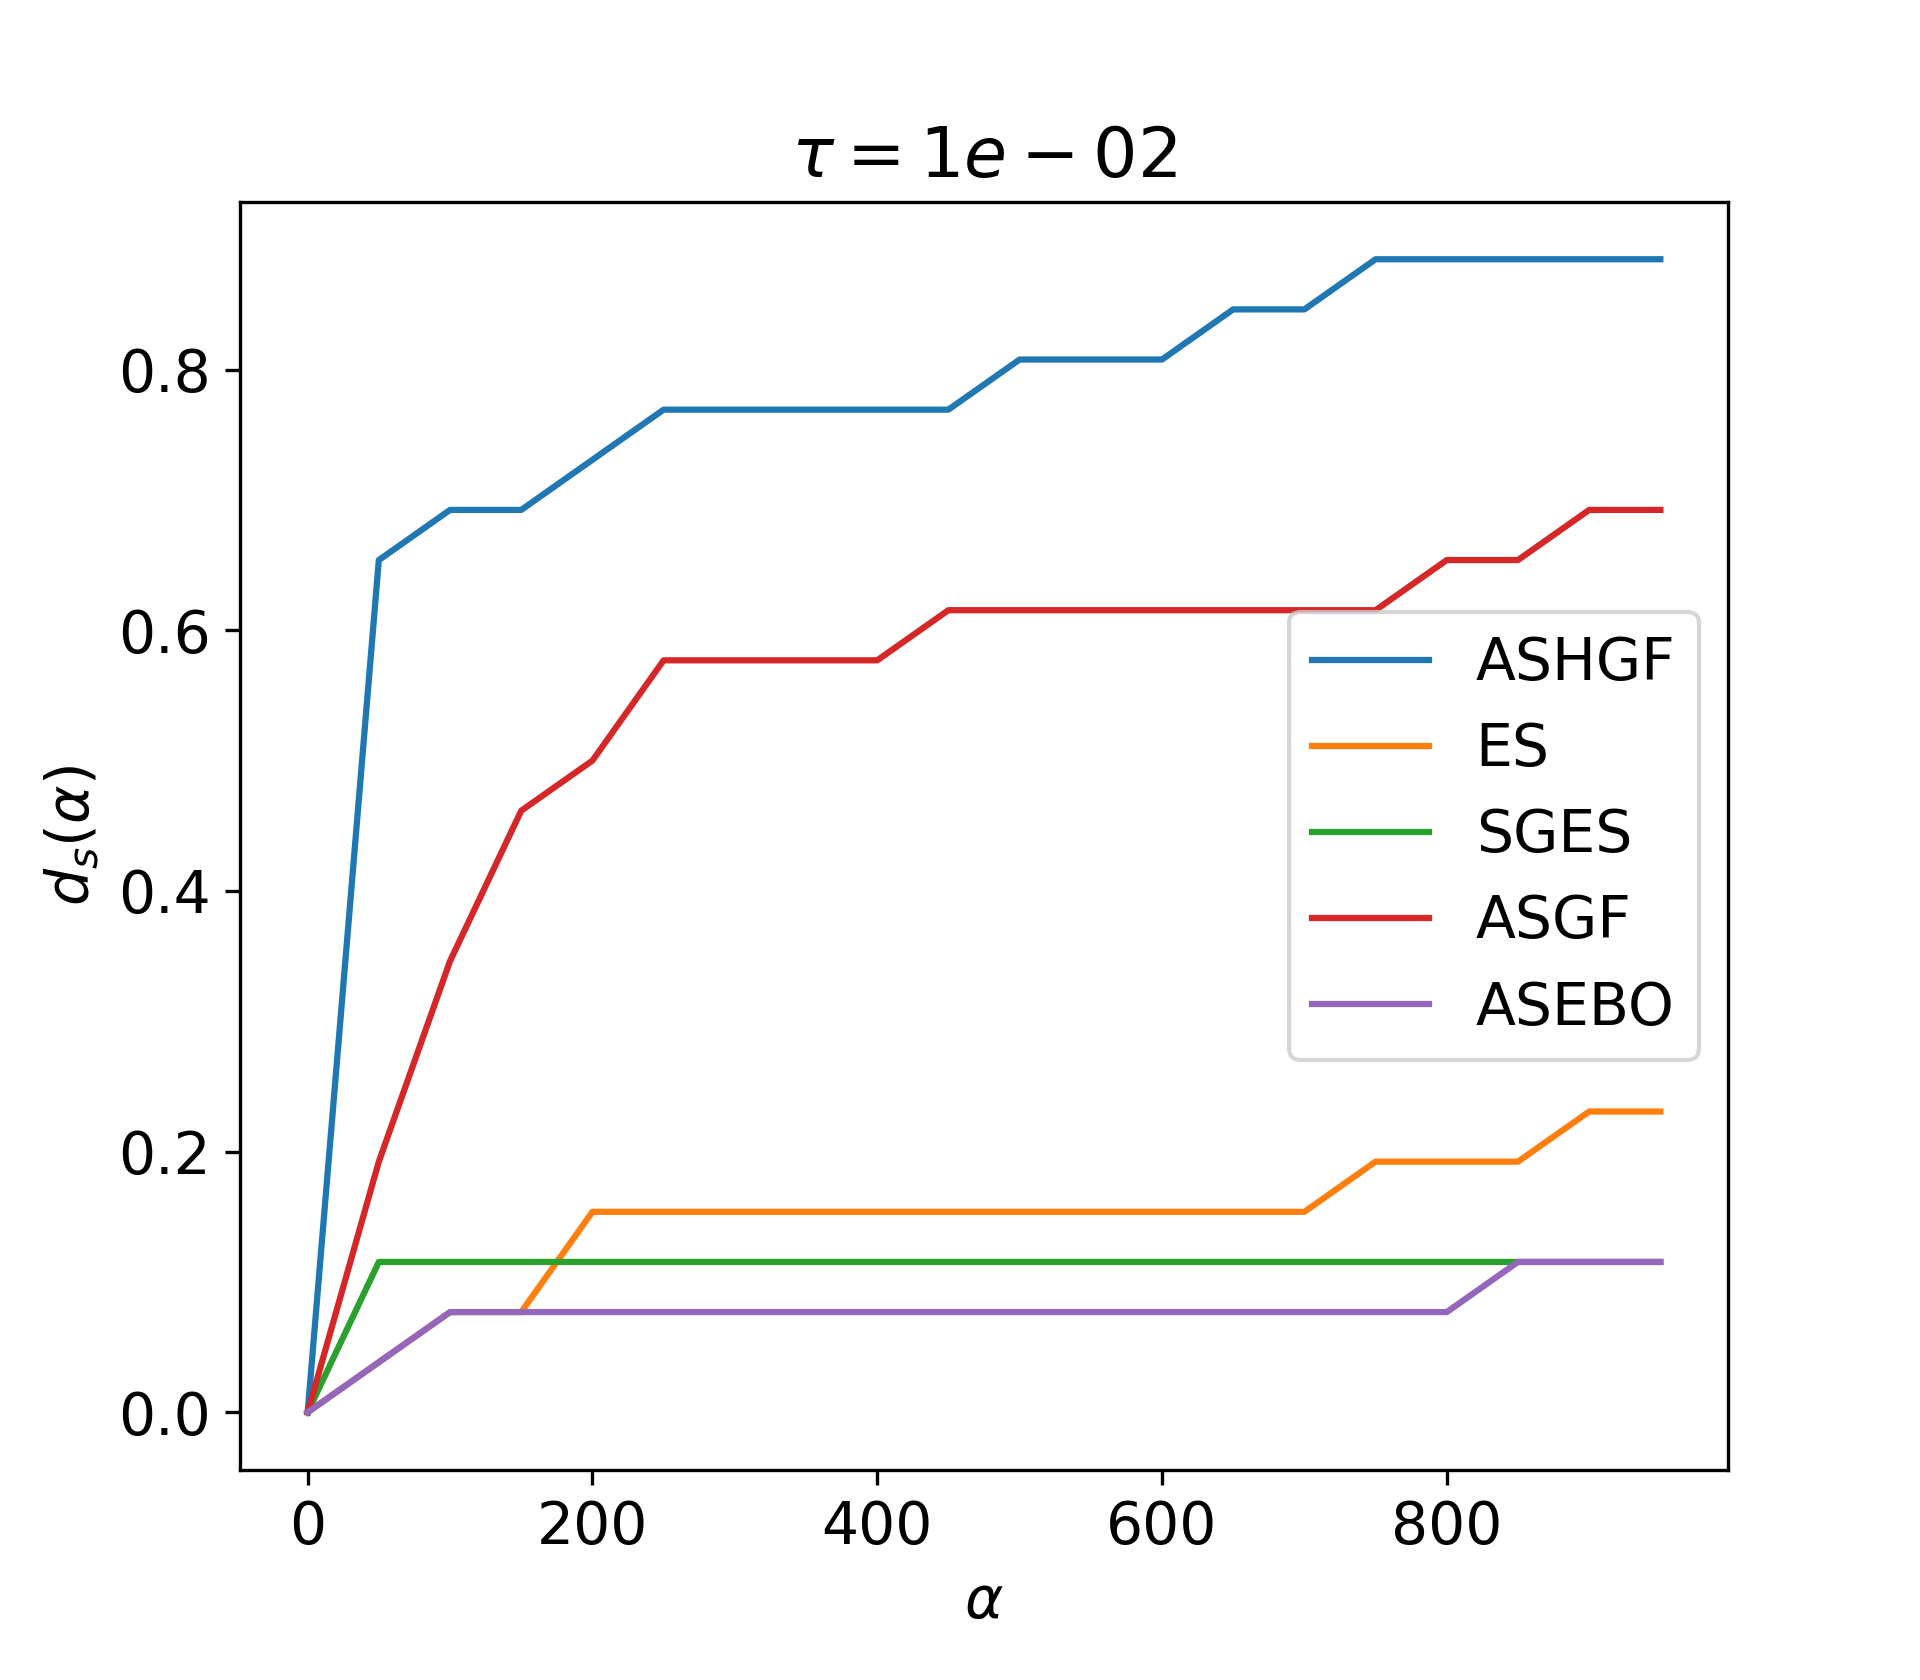
\includegraphics[width=1\textwidth]{figures/data_profiles/10/data_profile_10_10000_1e-02.png}
\end{subfigure}%
\begin{subfigure}{0.3\textwidth}
  \centering 
  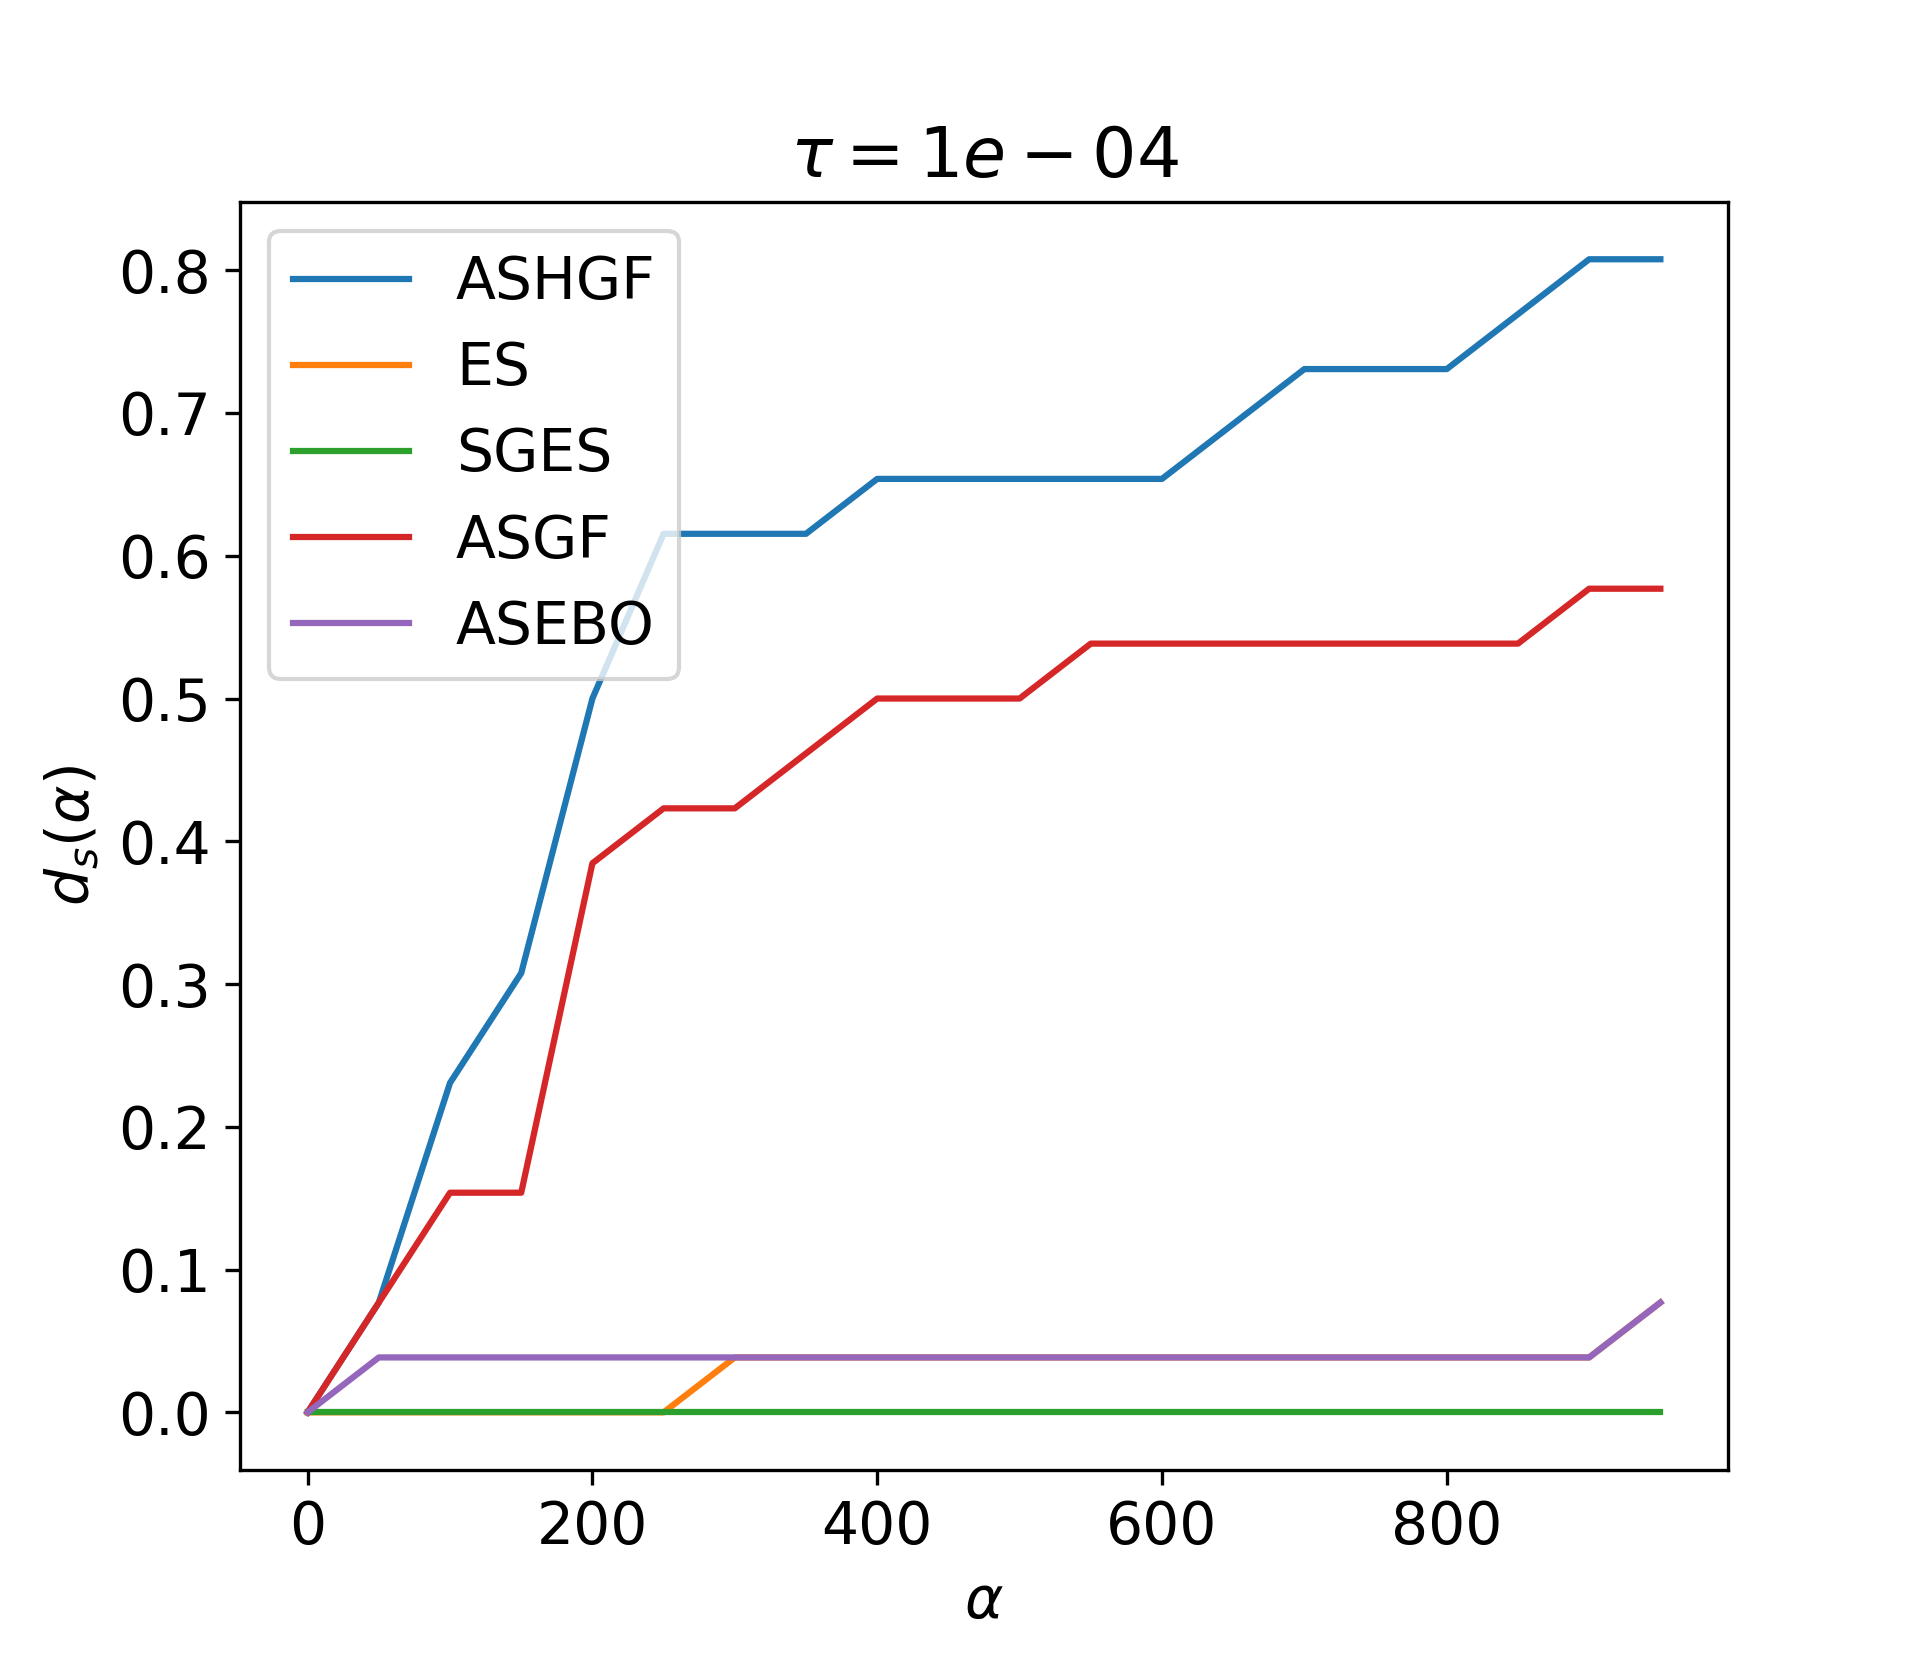
\includegraphics[width=1\textwidth]{figures/data_profiles/10/data_profile_10_10000_1e-04.png}
\end{subfigure}
\begin{subfigure}{0.3\textwidth}
  \centering 
  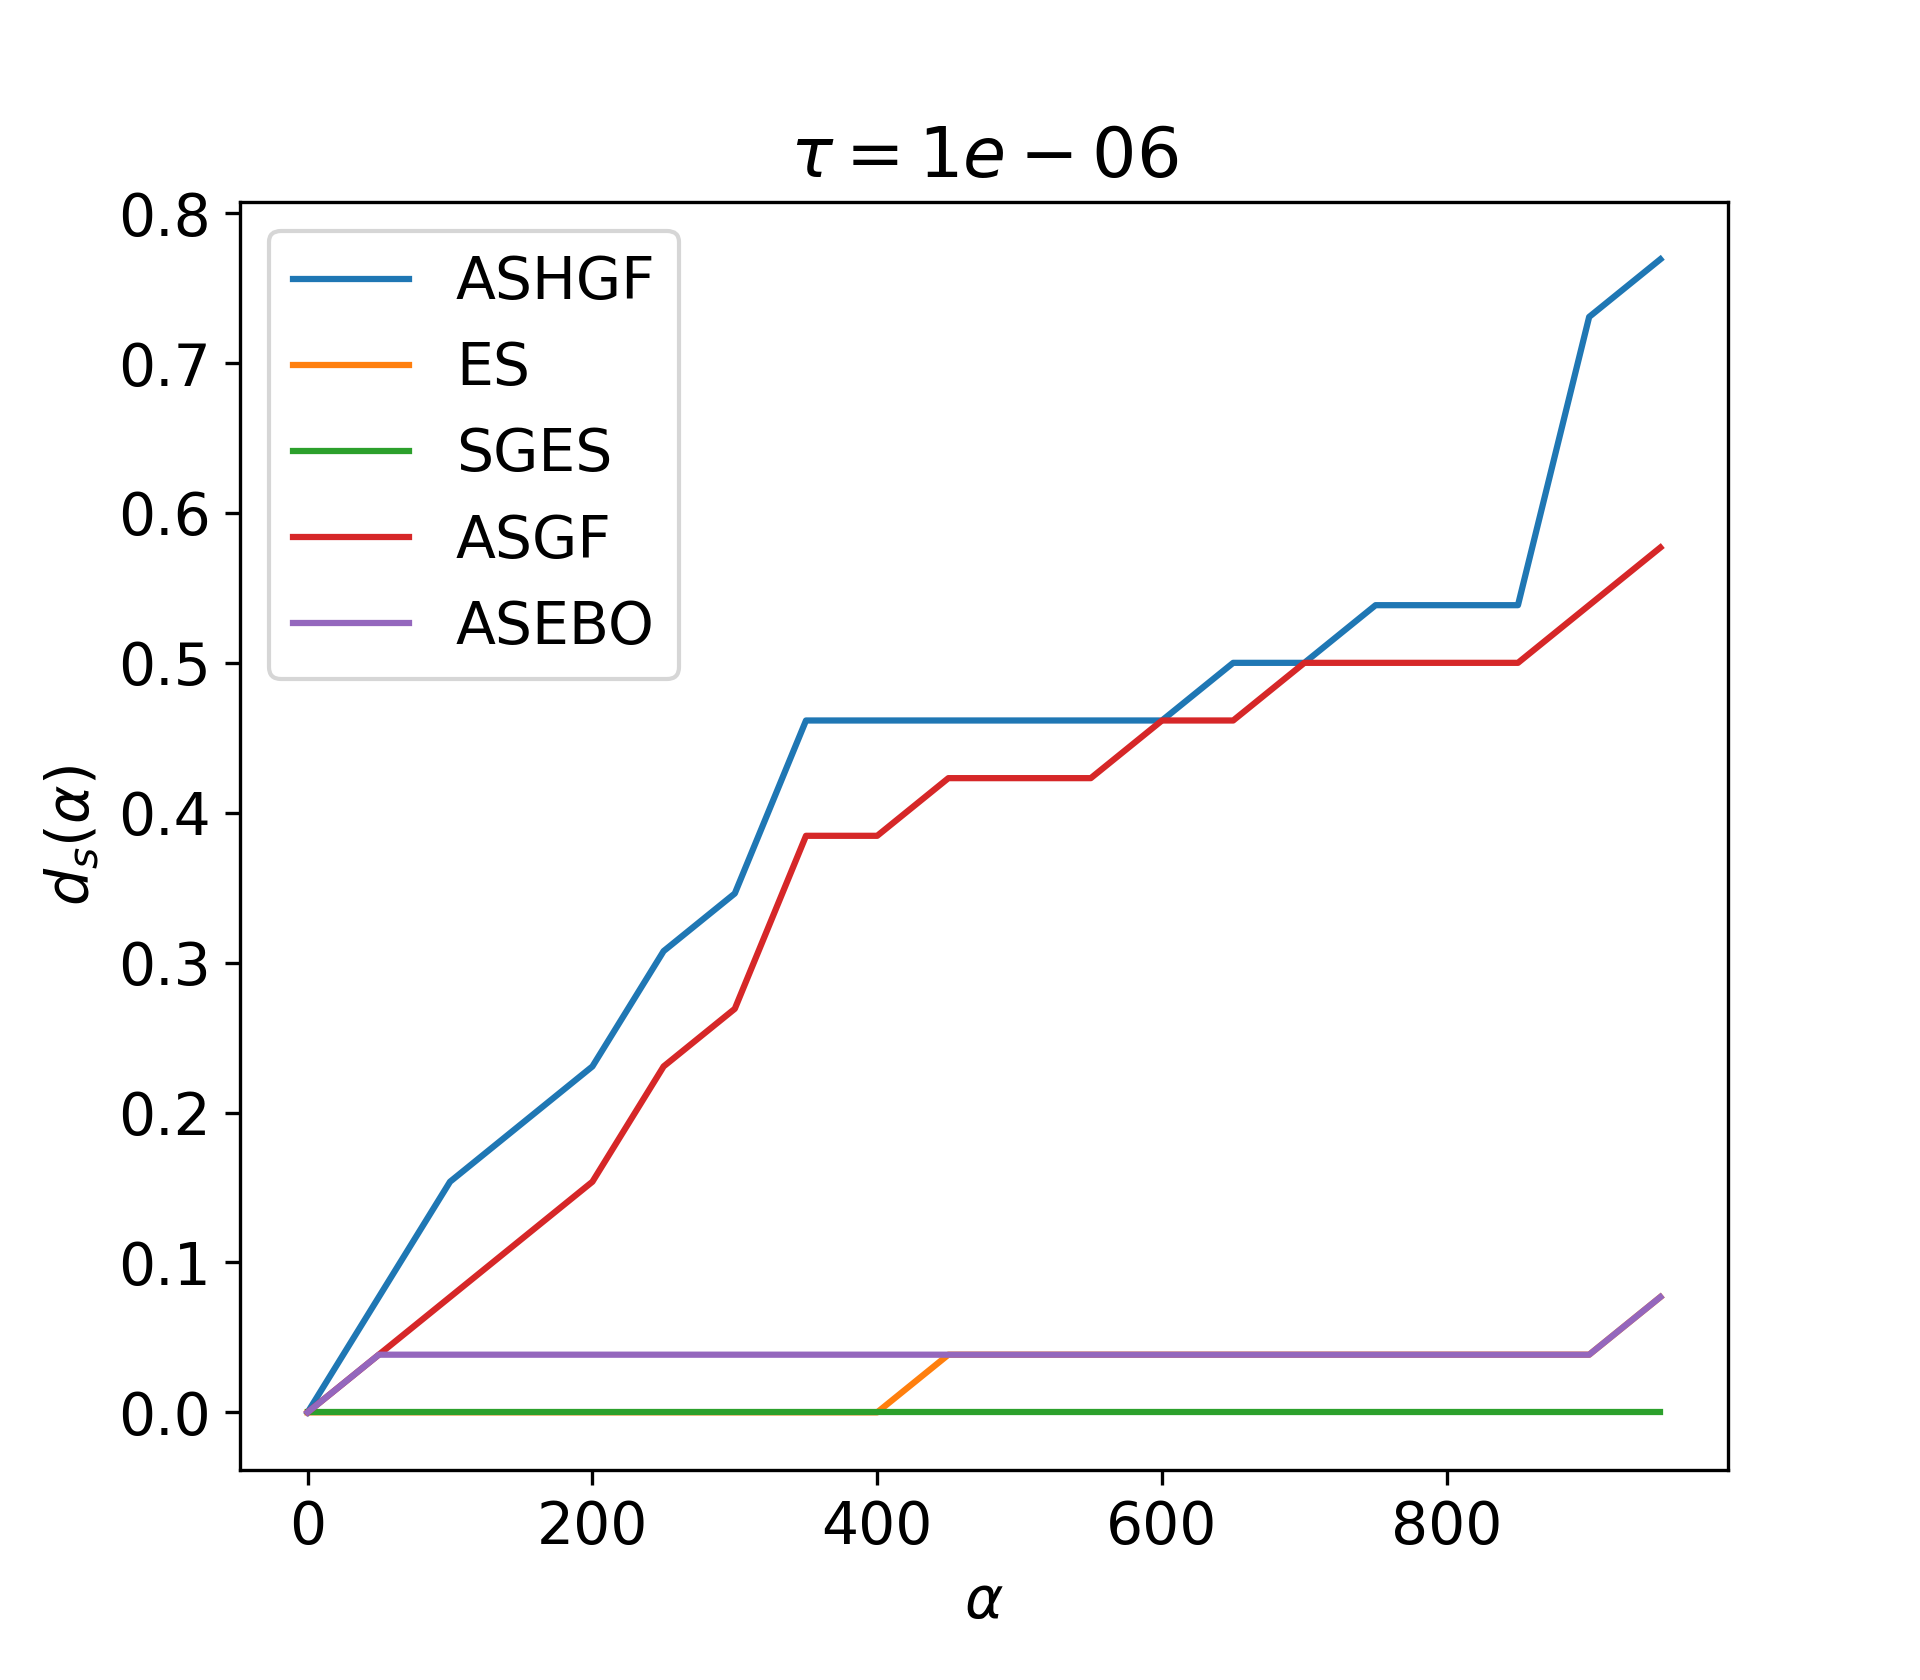
\includegraphics[width=1\textwidth]{figures/data_profiles/10/data_profile_10_10000_1e-06.png}
\end{subfigure}
\centering
\begin{subfigure}{0.3\textwidth}
  \centering 
  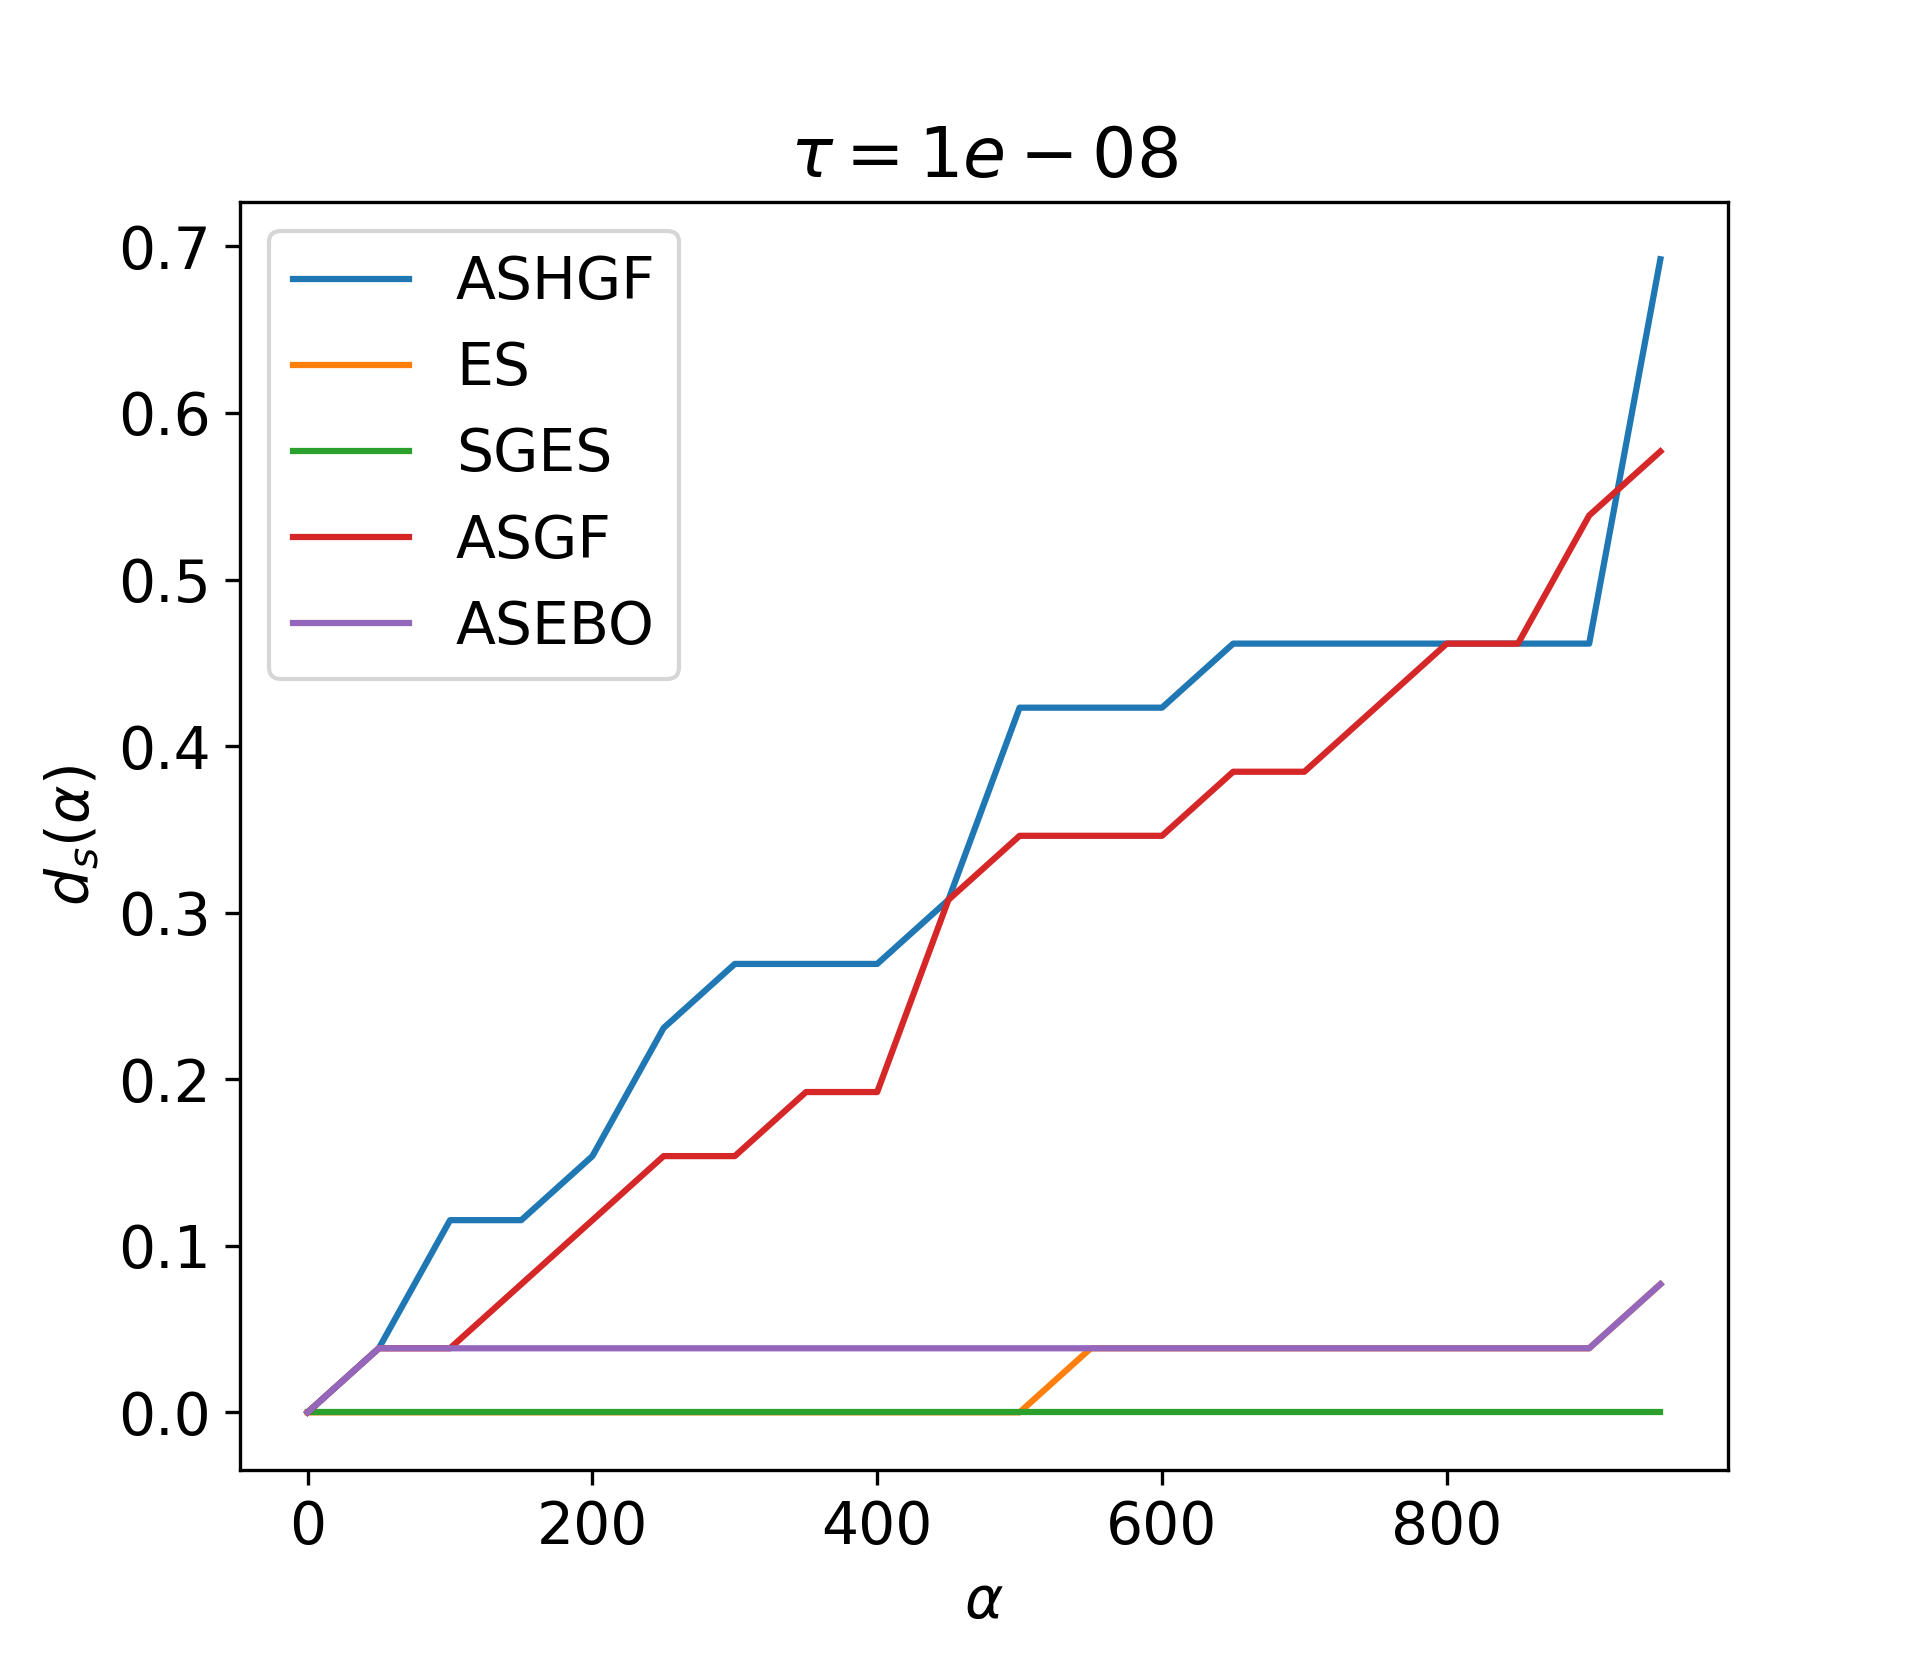
\includegraphics[width=1\textwidth]{figures/data_profiles/10/data_profile_10_10000_1e-08.png}
\end{subfigure}%
\begin{subfigure}{0.3\textwidth}
  \centering 
  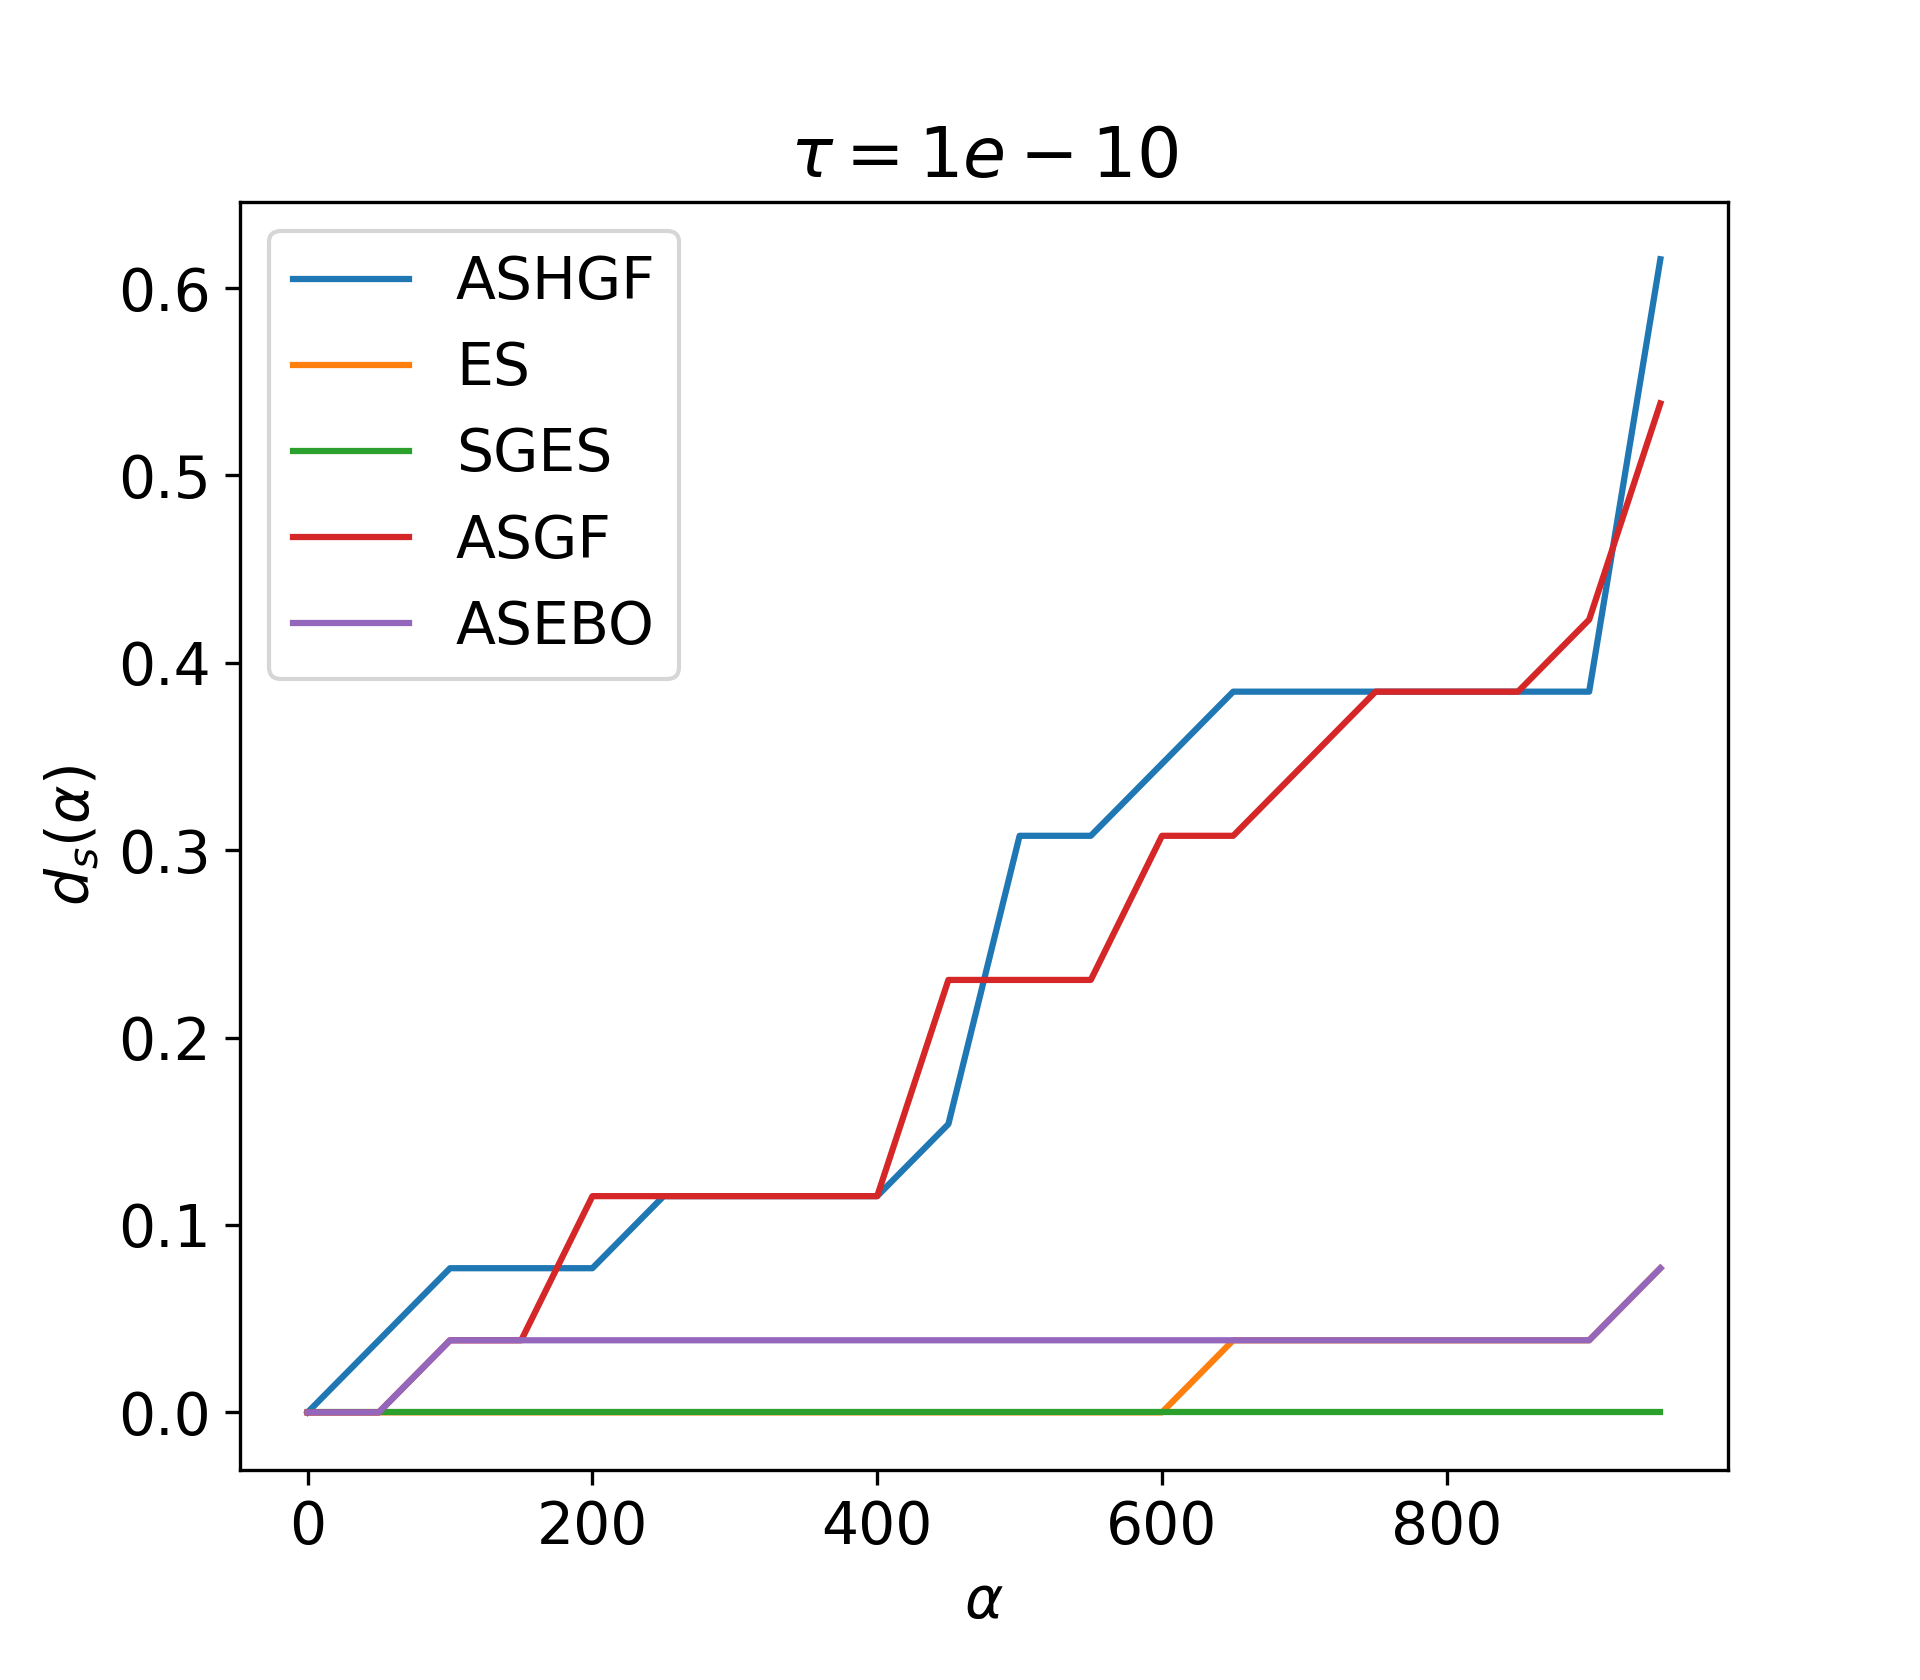
\includegraphics[width=1\textwidth]{figures/data_profiles/10/data_profile_10_10000_1e-10.png}
\end{subfigure}
\caption{Data profiles with $\mu_L = 10^{4}$}
\label{DataProfiles10Mu10000}
\end{figure}

\begin{figure}[H]
\centering
\begin{subfigure}{0.3\textwidth}
  \centering 
  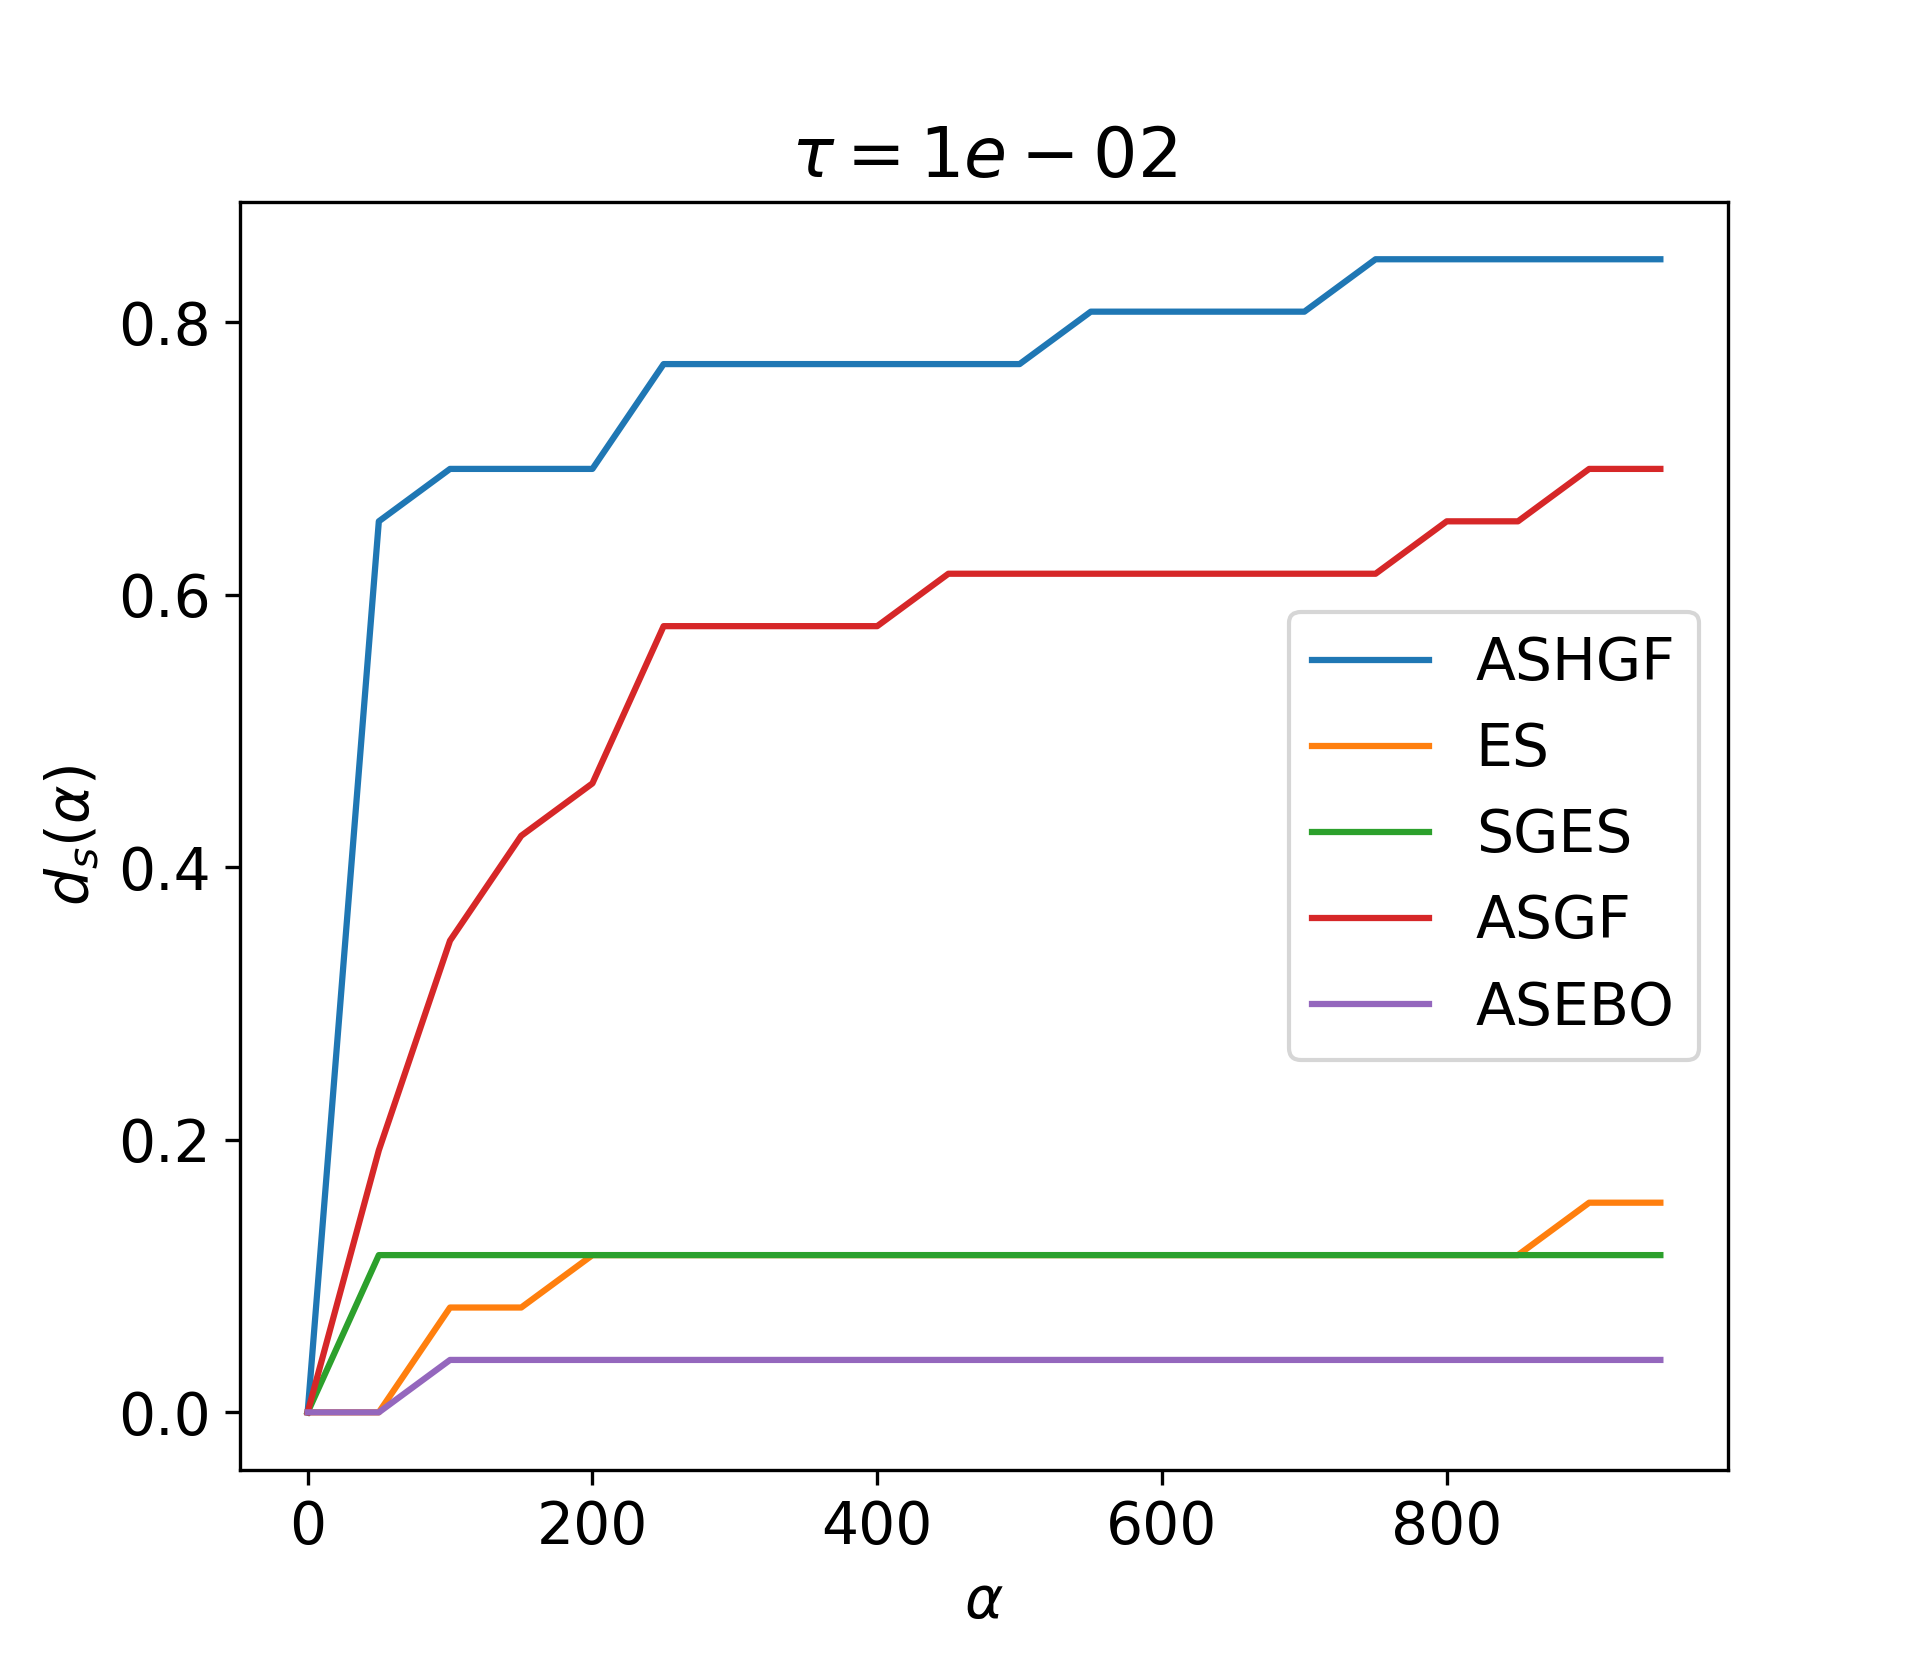
\includegraphics[width=1\textwidth]{figures/data_profiles/10/data_profile_10_100000_1e-02.png}
\end{subfigure}%
\begin{subfigure}{0.3\textwidth}
  \centering 
  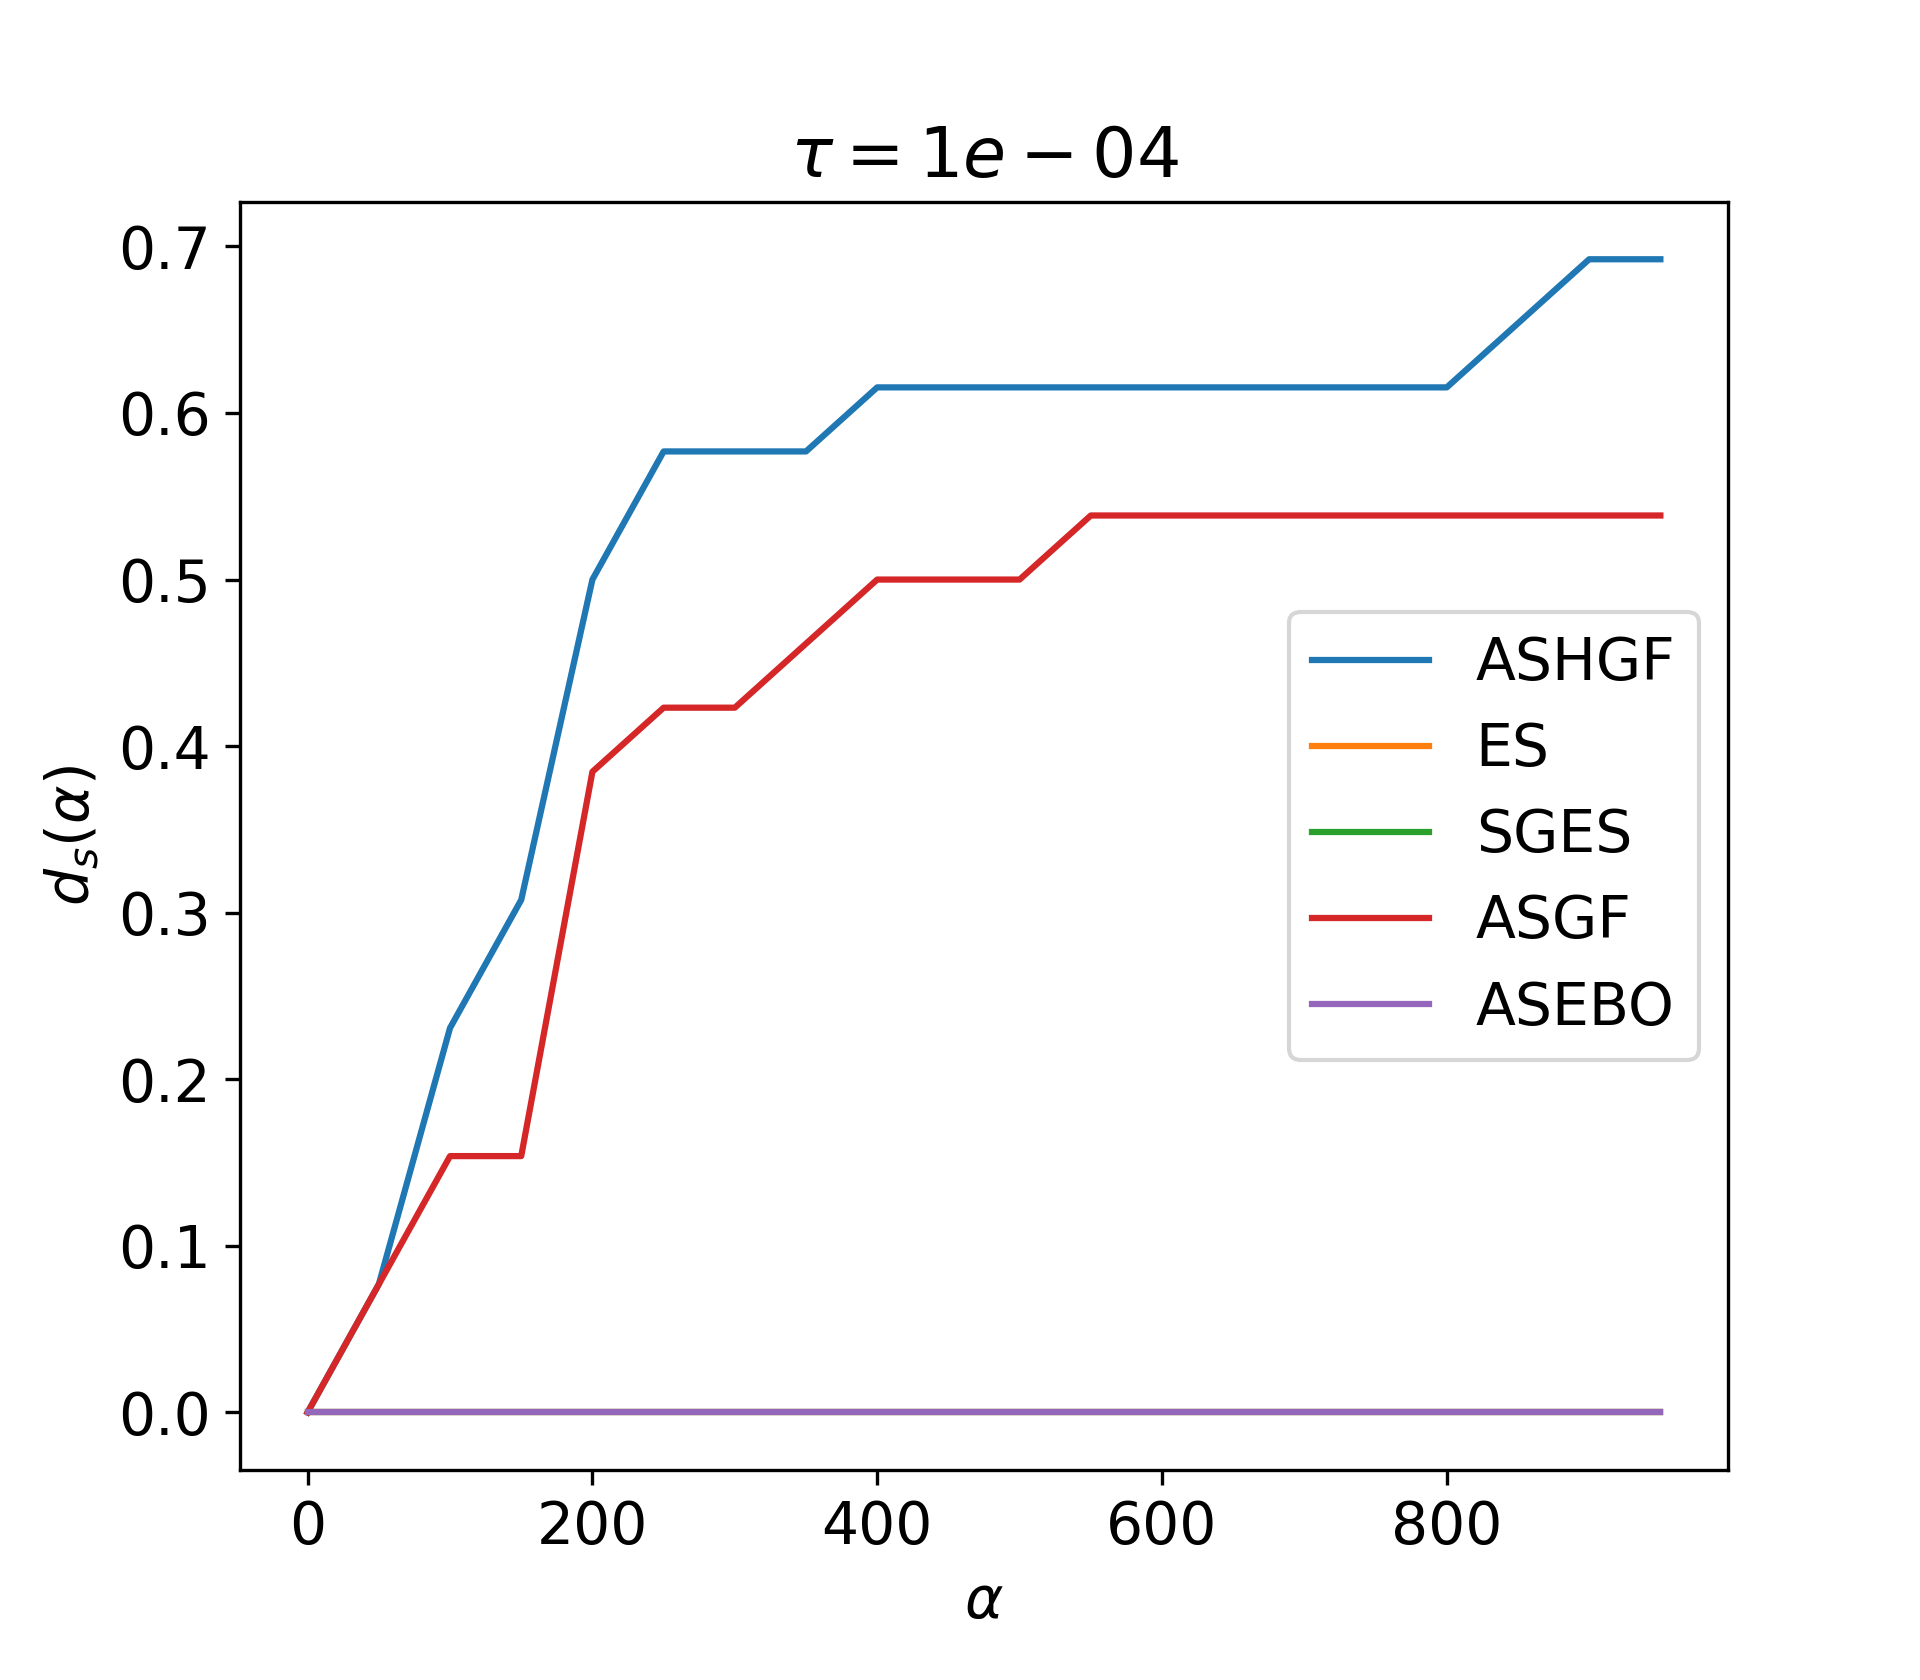
\includegraphics[width=1\textwidth]{figures/data_profiles/10/data_profile_10_100000_1e-04.png}
\end{subfigure}
\begin{subfigure}{0.3\textwidth}
  \centering 
  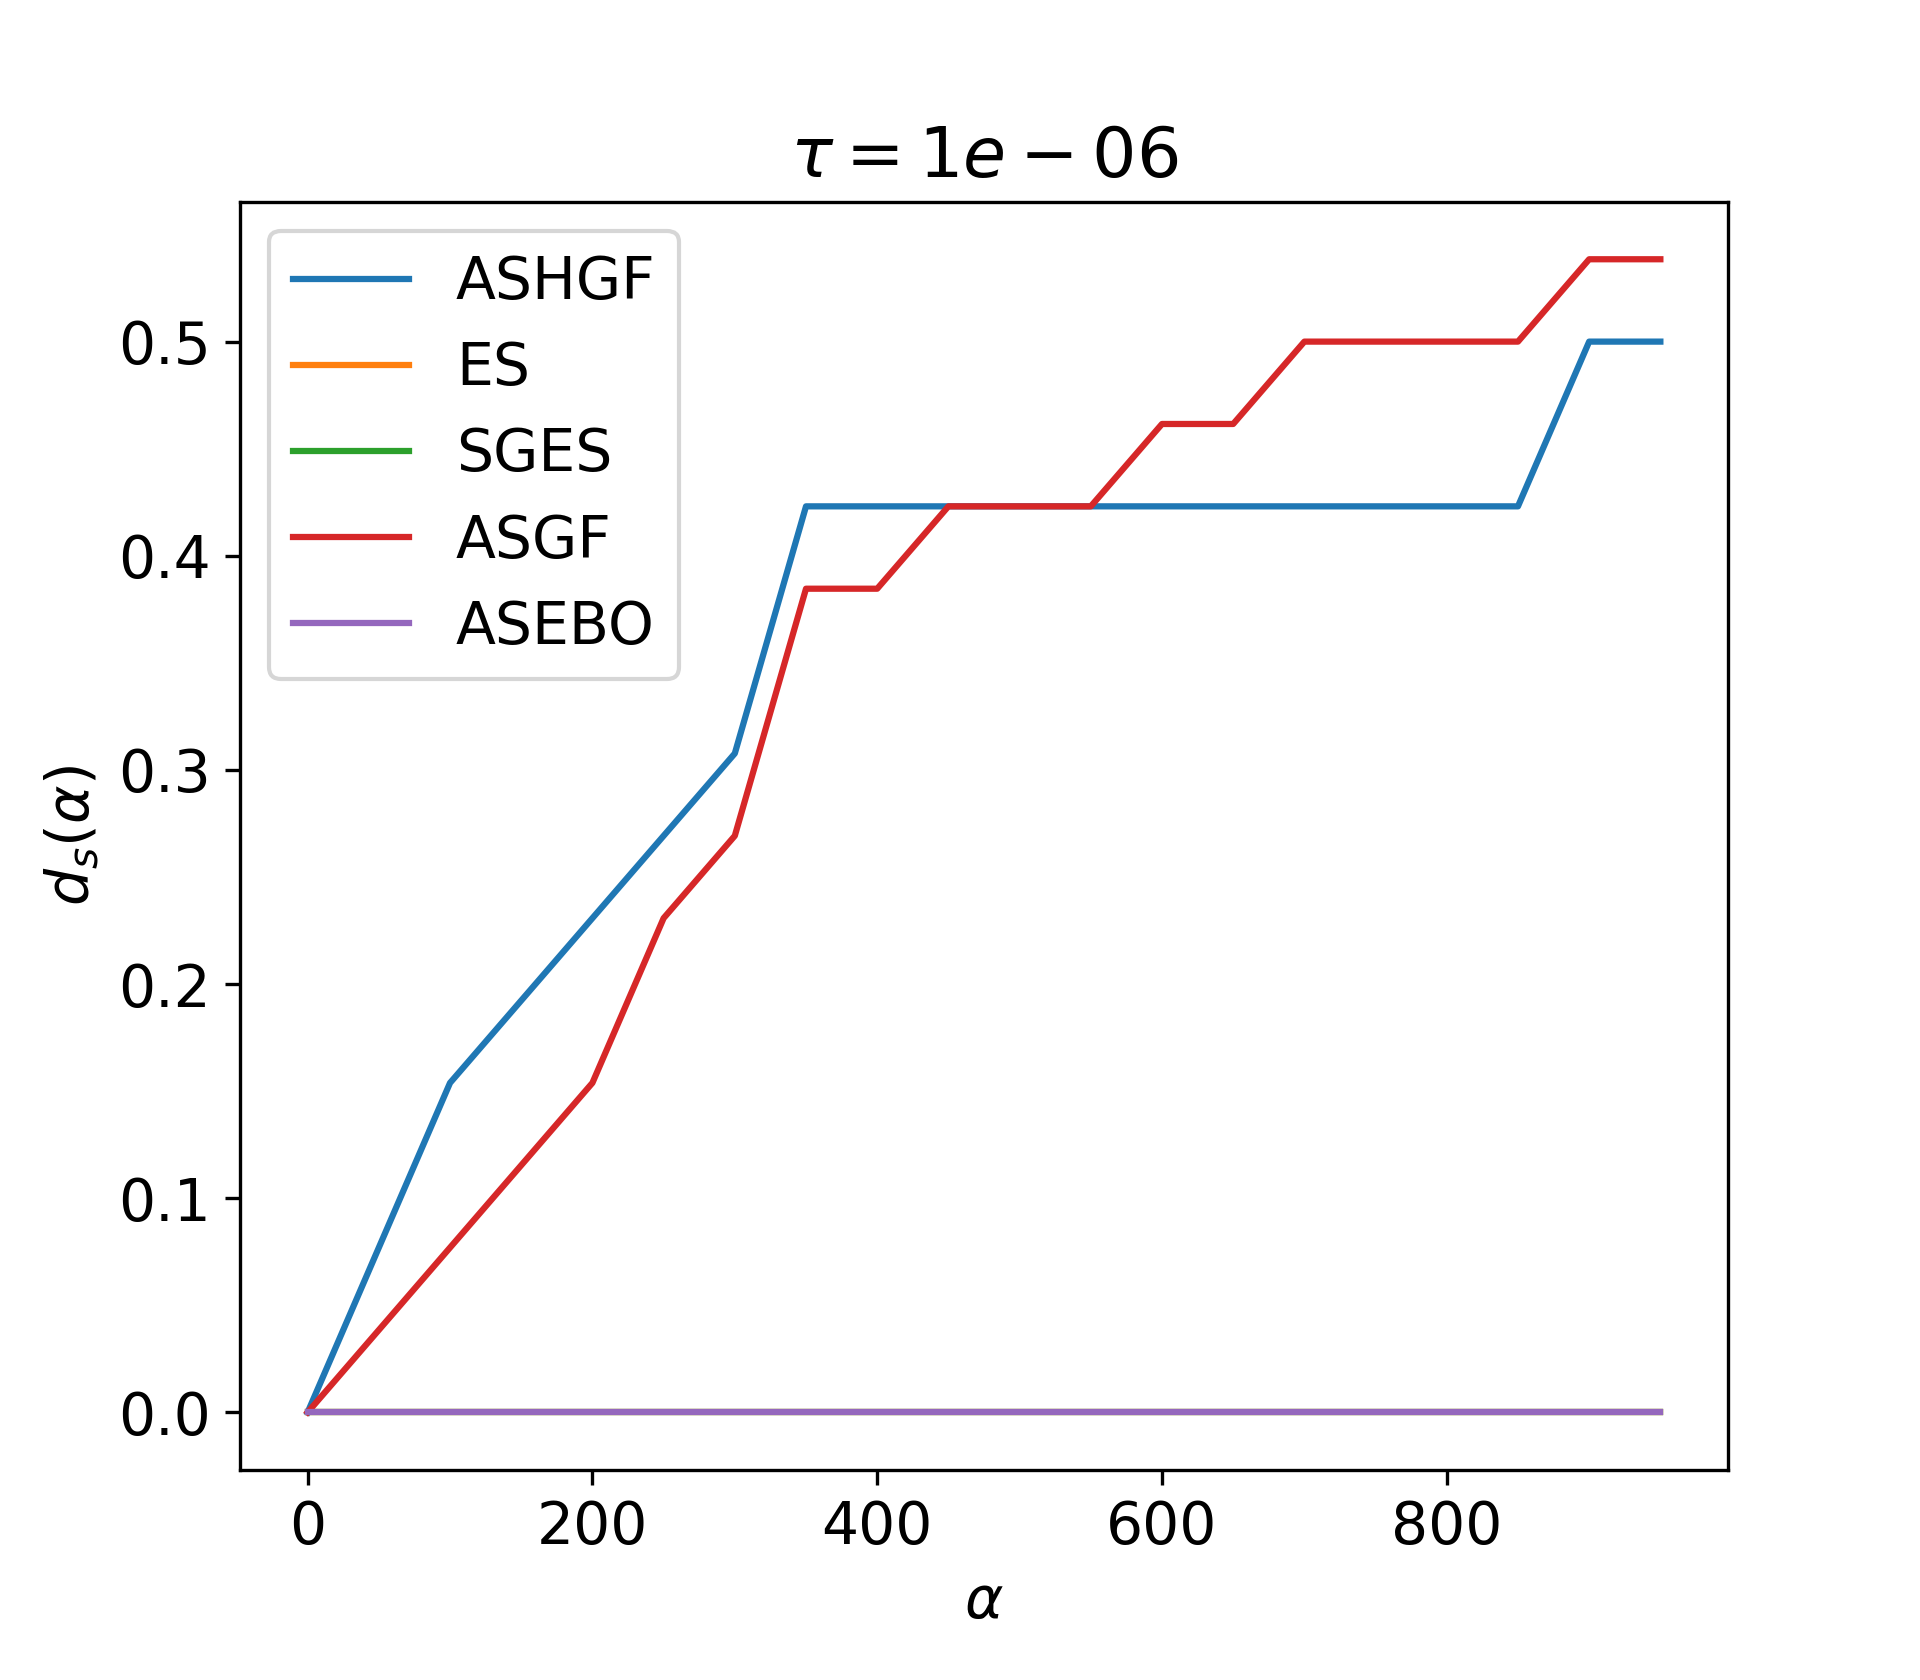
\includegraphics[width=1\textwidth]{figures/data_profiles/10/data_profile_10_100000_1e-06.png}
\end{subfigure}
\centering
\begin{subfigure}{0.3\textwidth}
  \centering 
  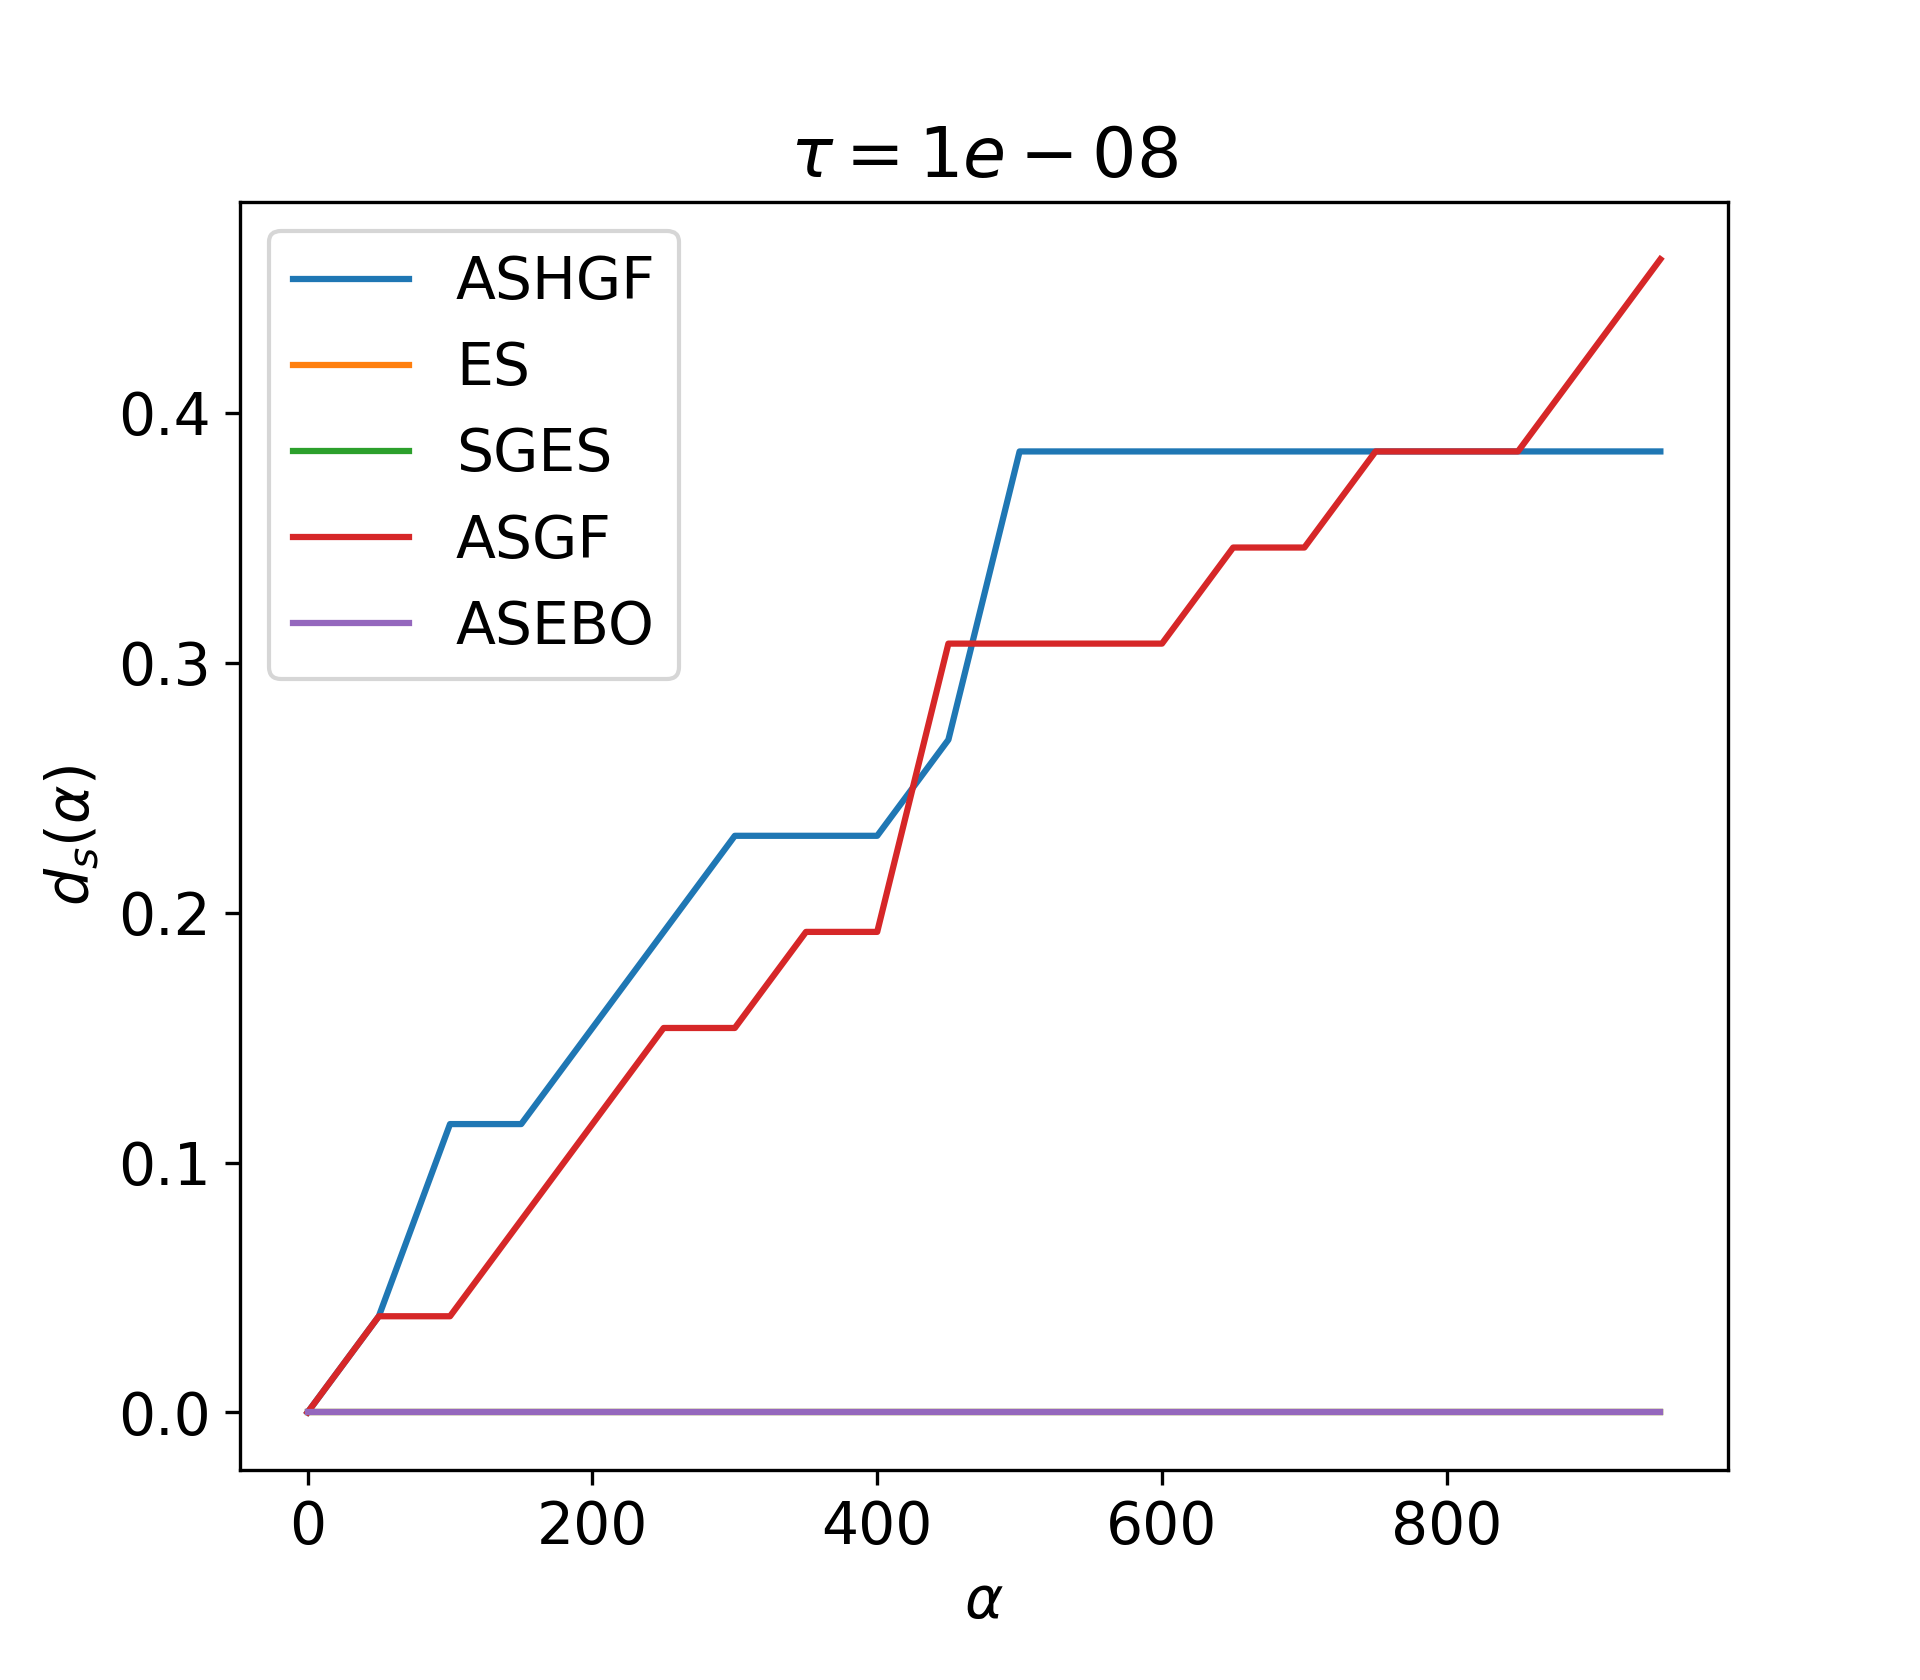
\includegraphics[width=1\textwidth]{figures/data_profiles/10/data_profile_10_100000_1e-08.png}
\end{subfigure}%
\begin{subfigure}{0.3\textwidth}
  \centering 
  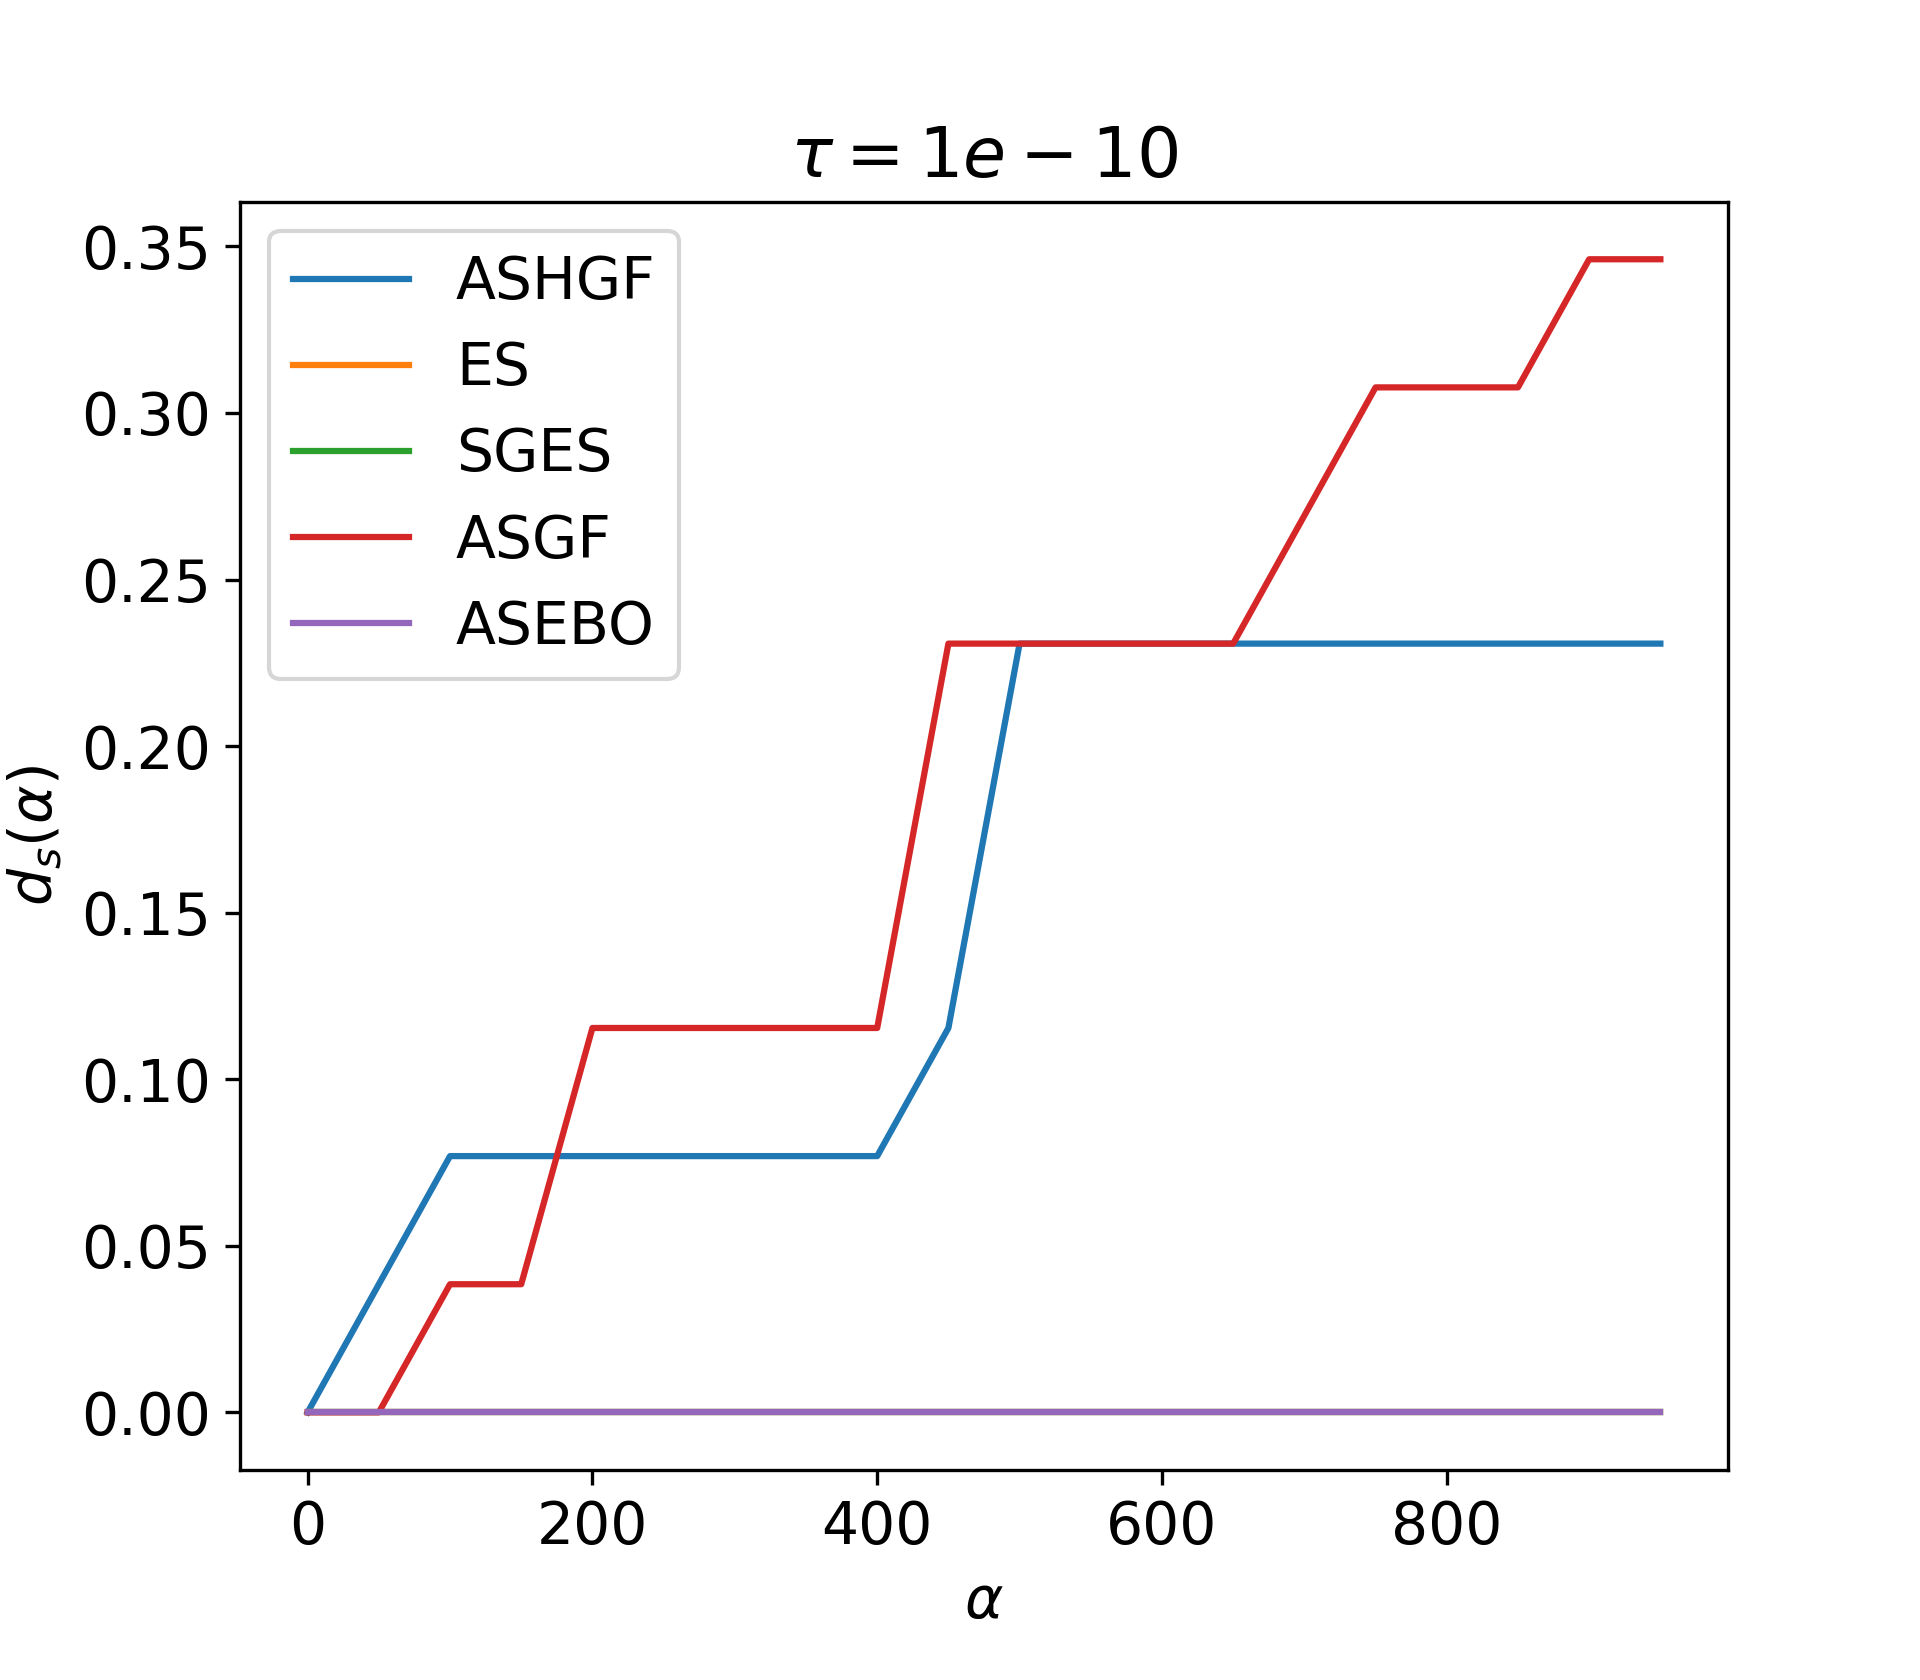
\includegraphics[width=1\textwidth]{figures/data_profiles/10/data_profile_10_100000_1e-10.png}
\end{subfigure}
\caption{Data profiles with $\mu_L = 10^{5}$}
\label{DataeProfiles10Mu100000}
\end{figure}

\begin{figure}[H]
\centering
\begin{subfigure}{0.3\textwidth}
  \centering 
  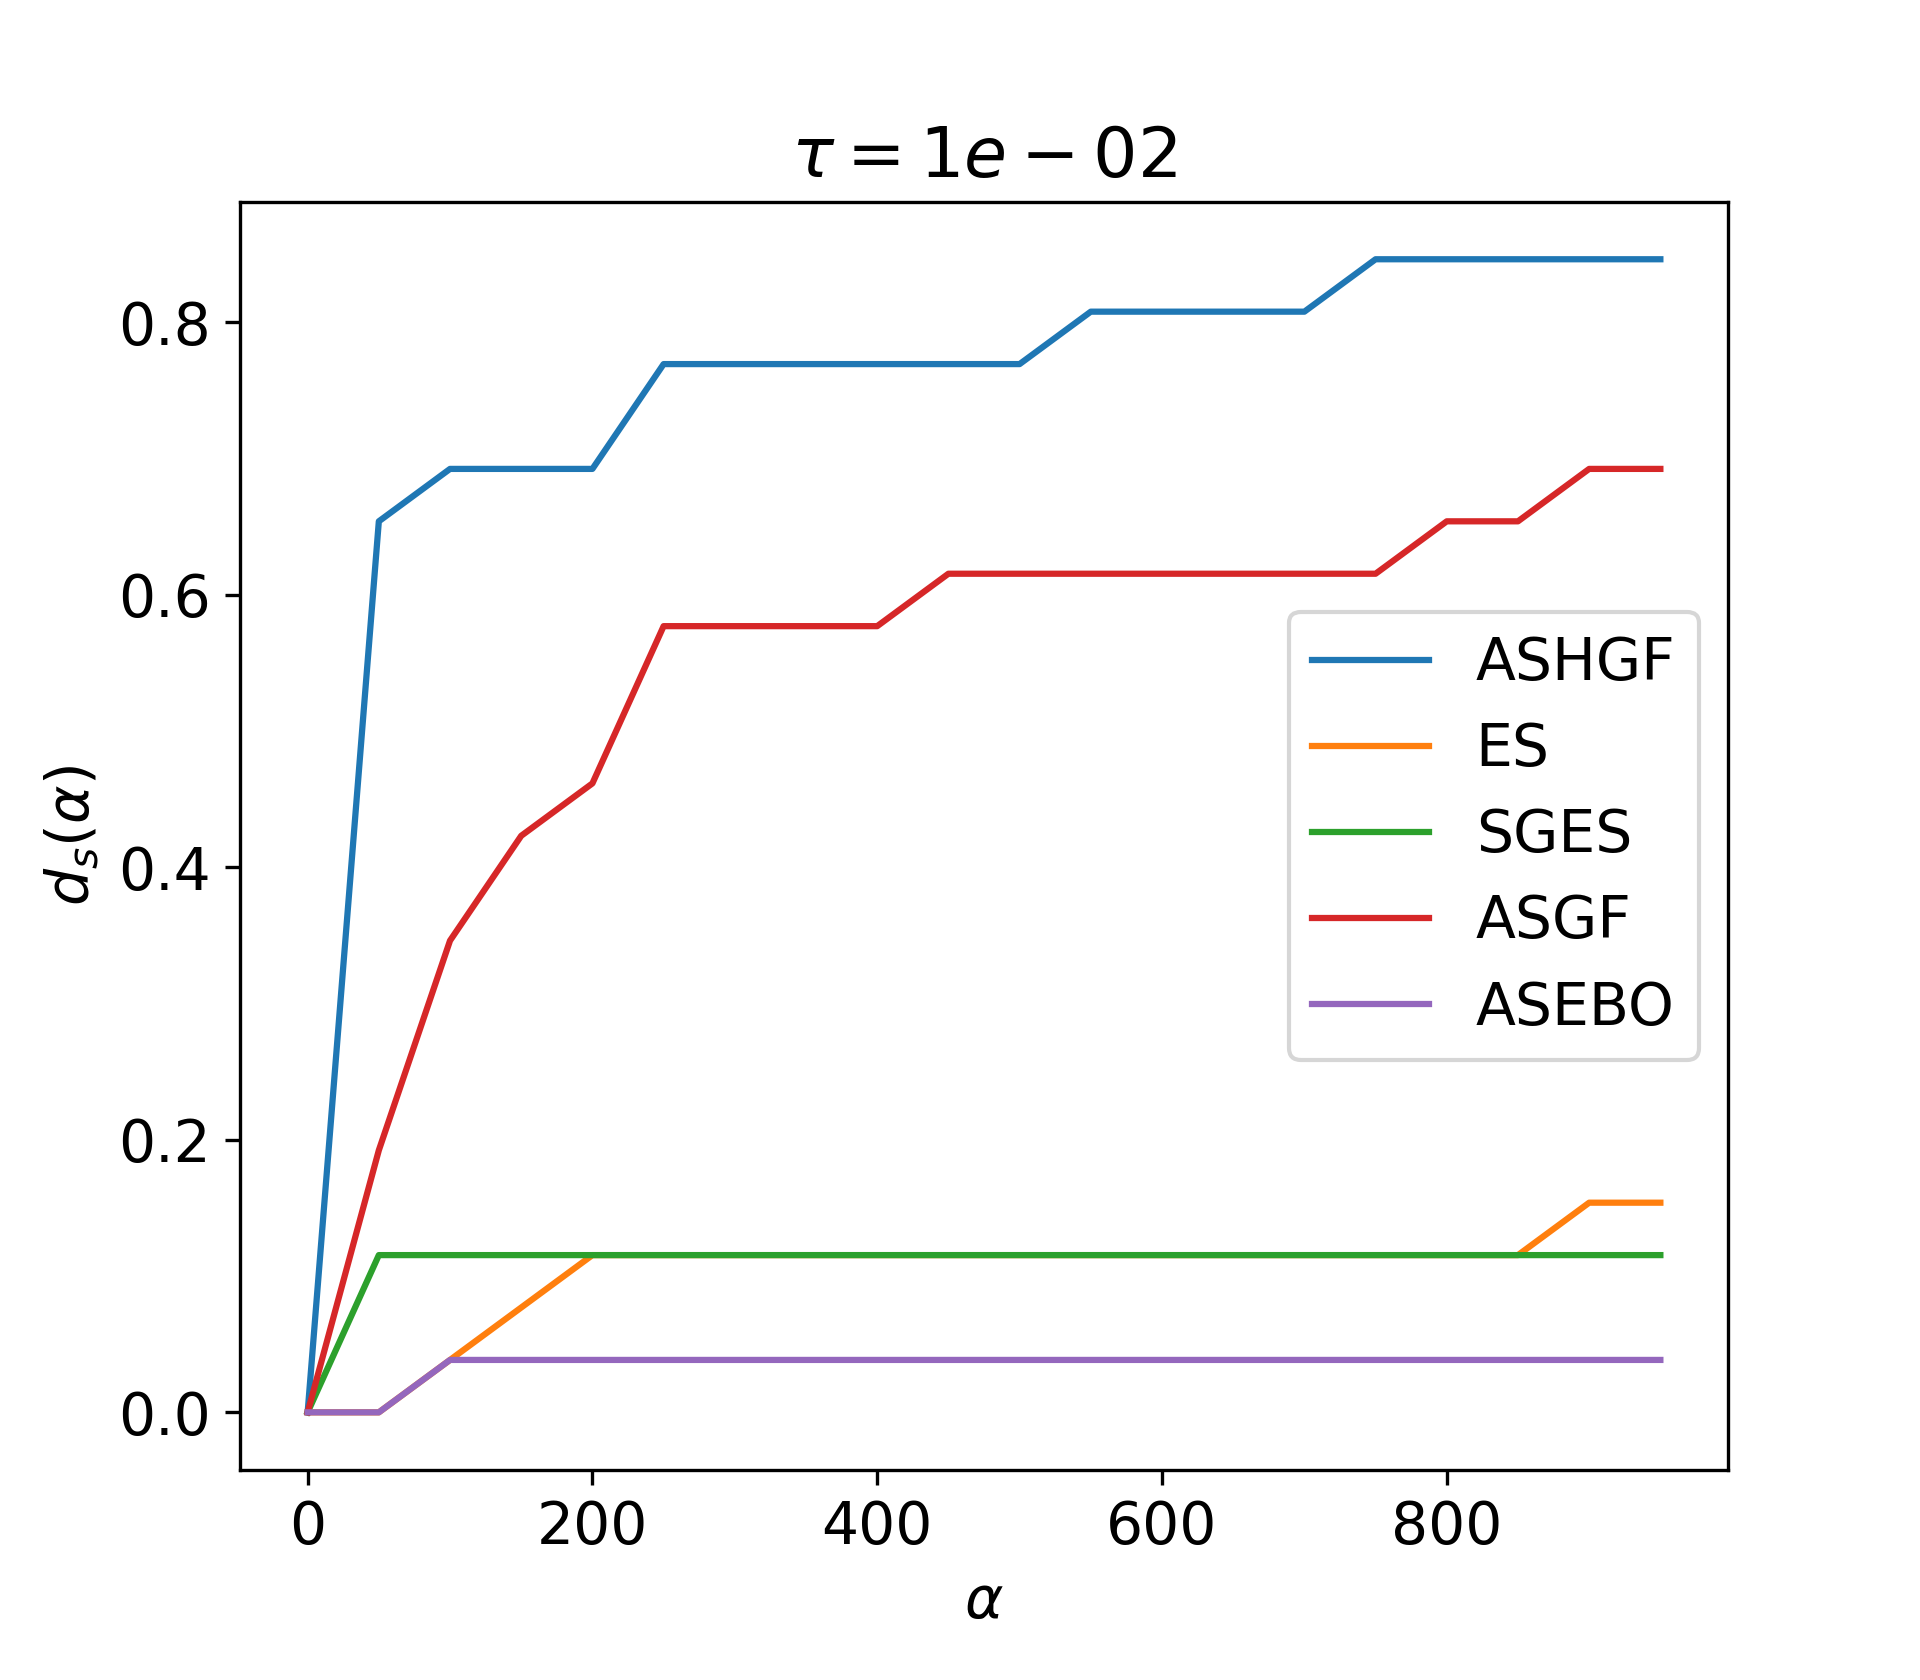
\includegraphics[width=1\textwidth]{figures/data_profiles/10/data_profile_10_1000000_1e-02.png}
\end{subfigure}%
\begin{subfigure}{0.3\textwidth}
  \centering 
  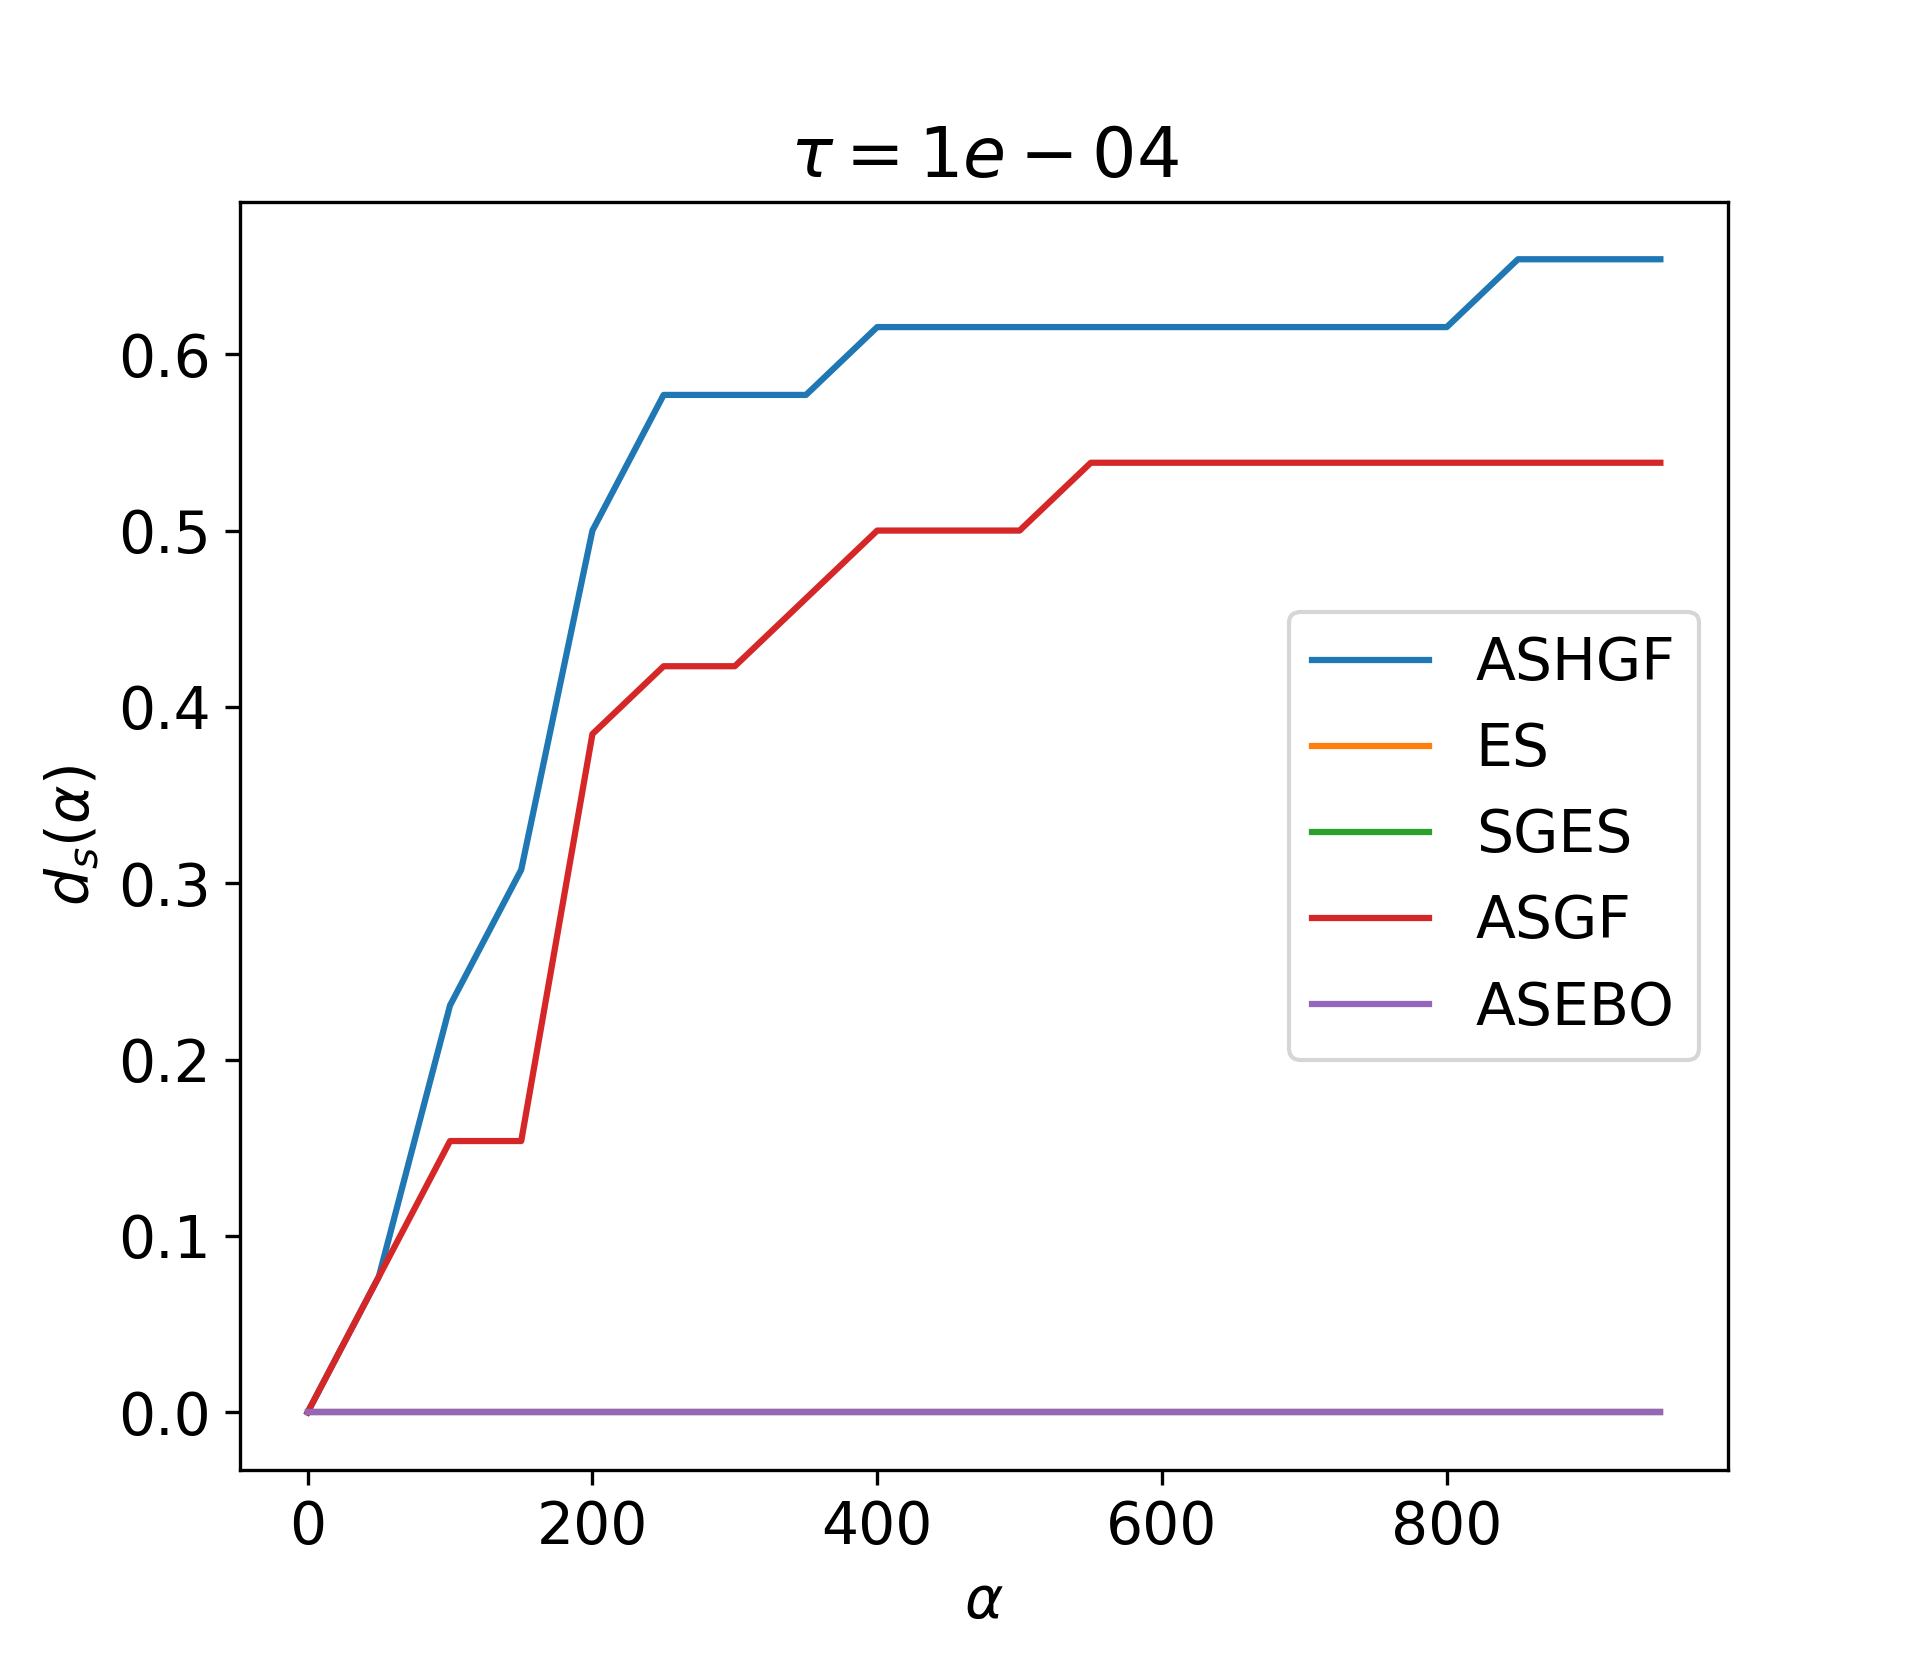
\includegraphics[width=1\textwidth]{figures/data_profiles/10/data_profile_10_1000000_1e-04.png}
\end{subfigure}
\begin{subfigure}{0.3\textwidth}
  \centering 
  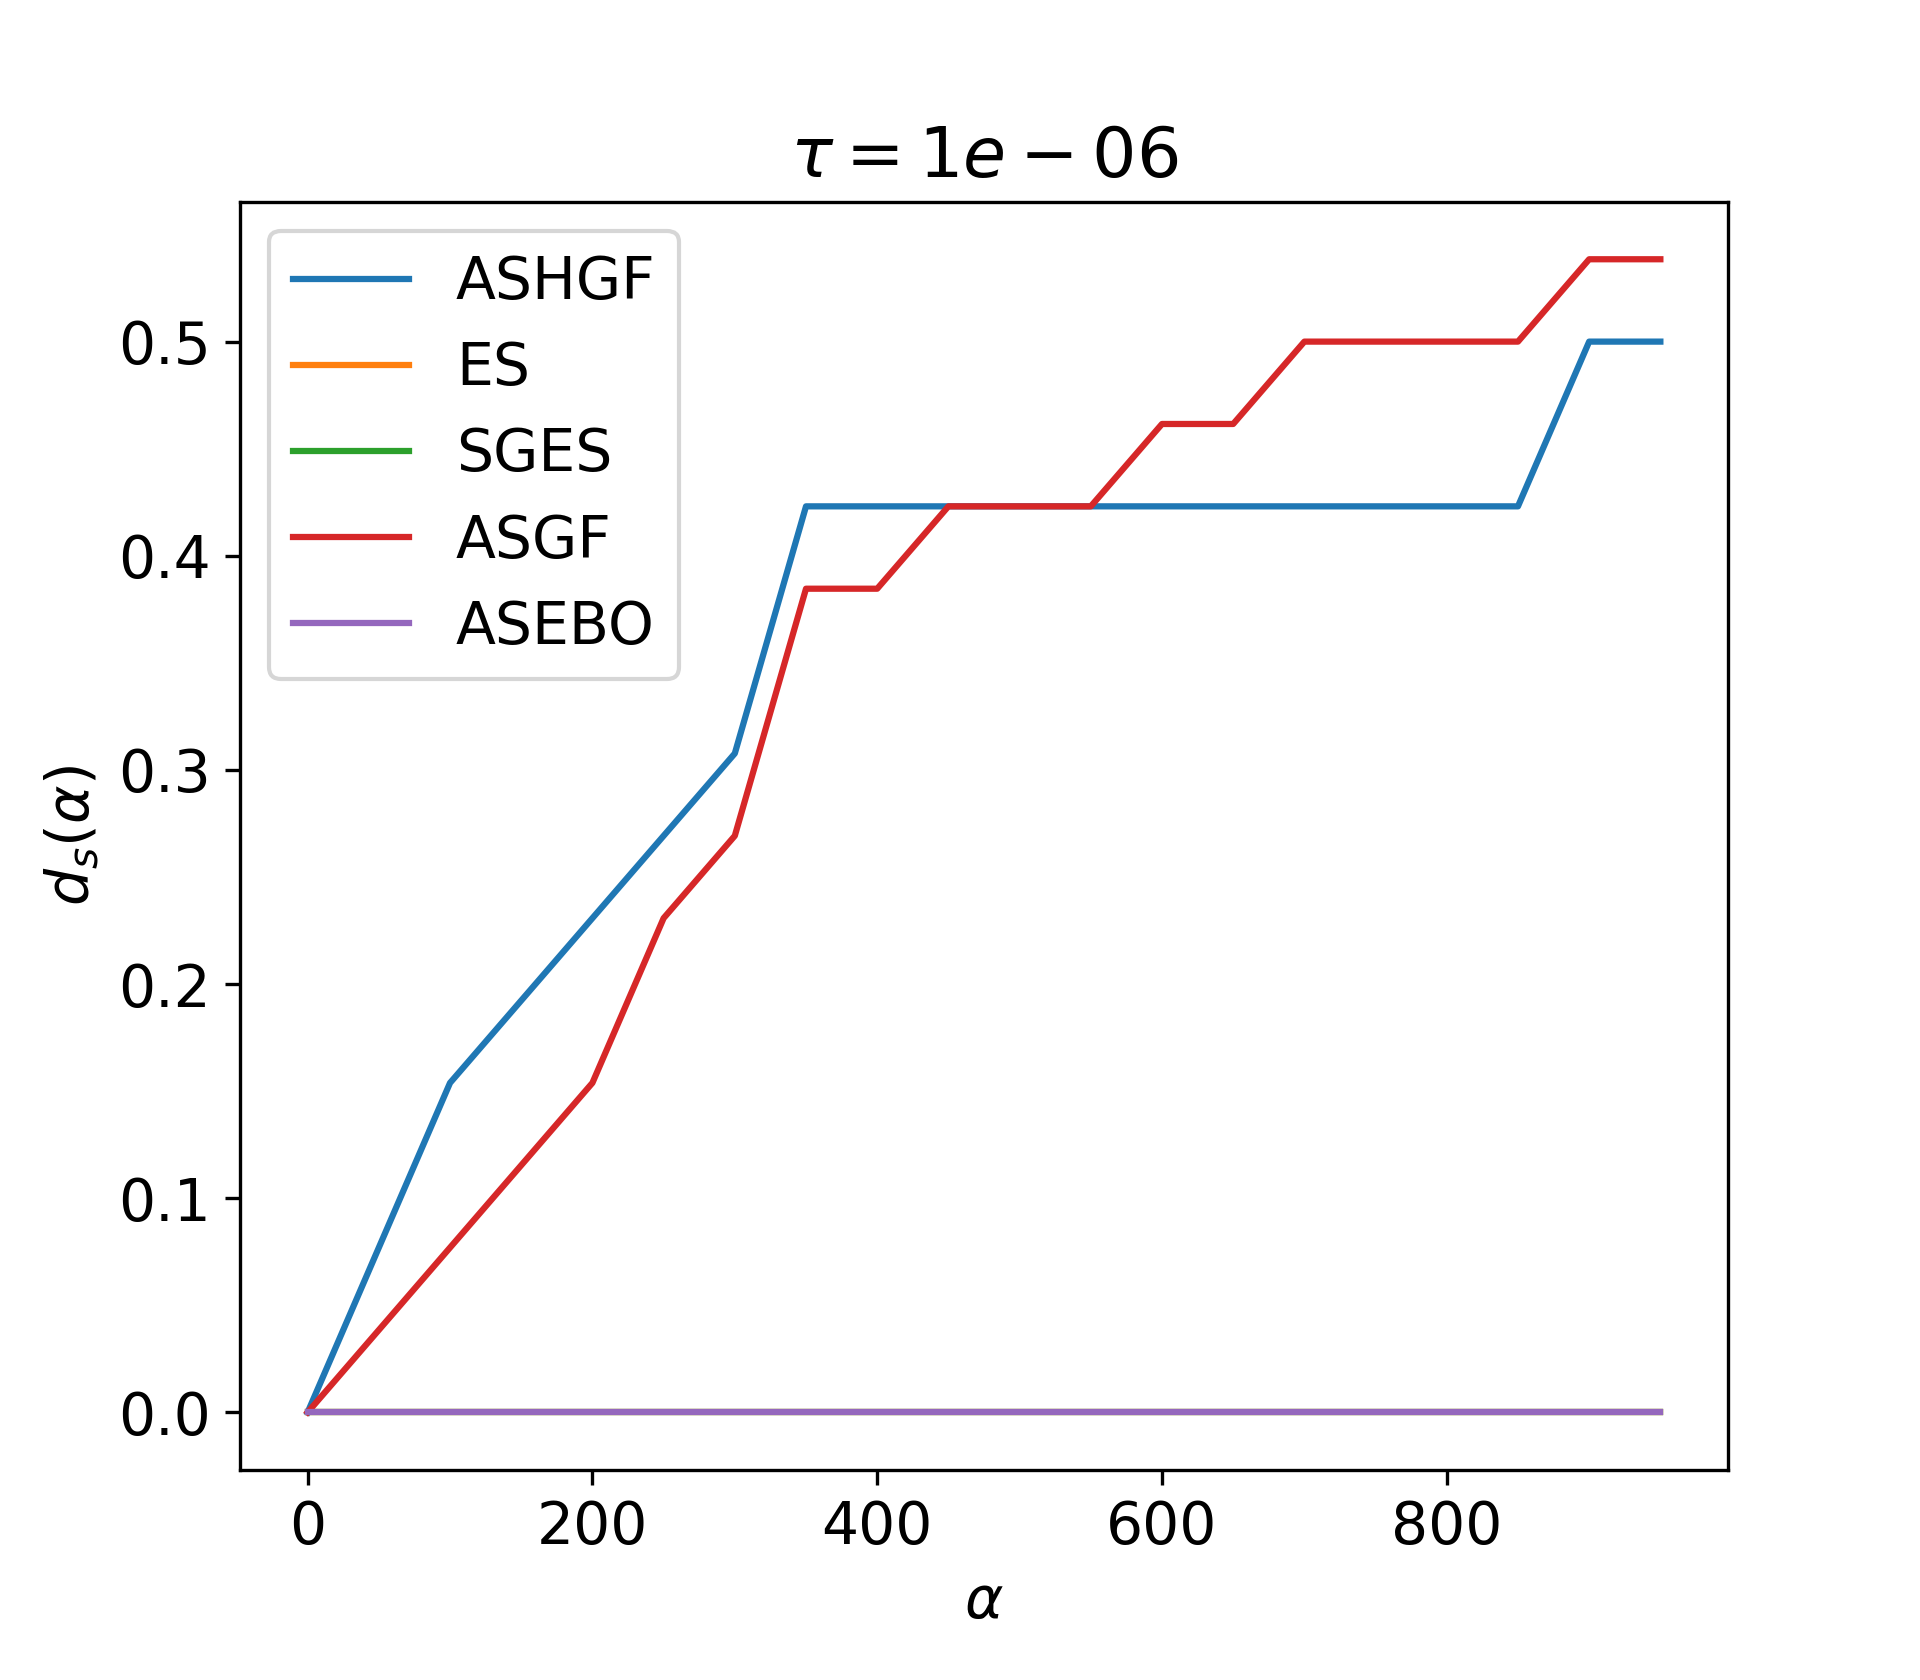
\includegraphics[width=1\textwidth]{figures/data_profiles/10/data_profile_10_1000000_1e-06.png}
\end{subfigure}
\centering
\begin{subfigure}{0.3\textwidth}
  \centering 
  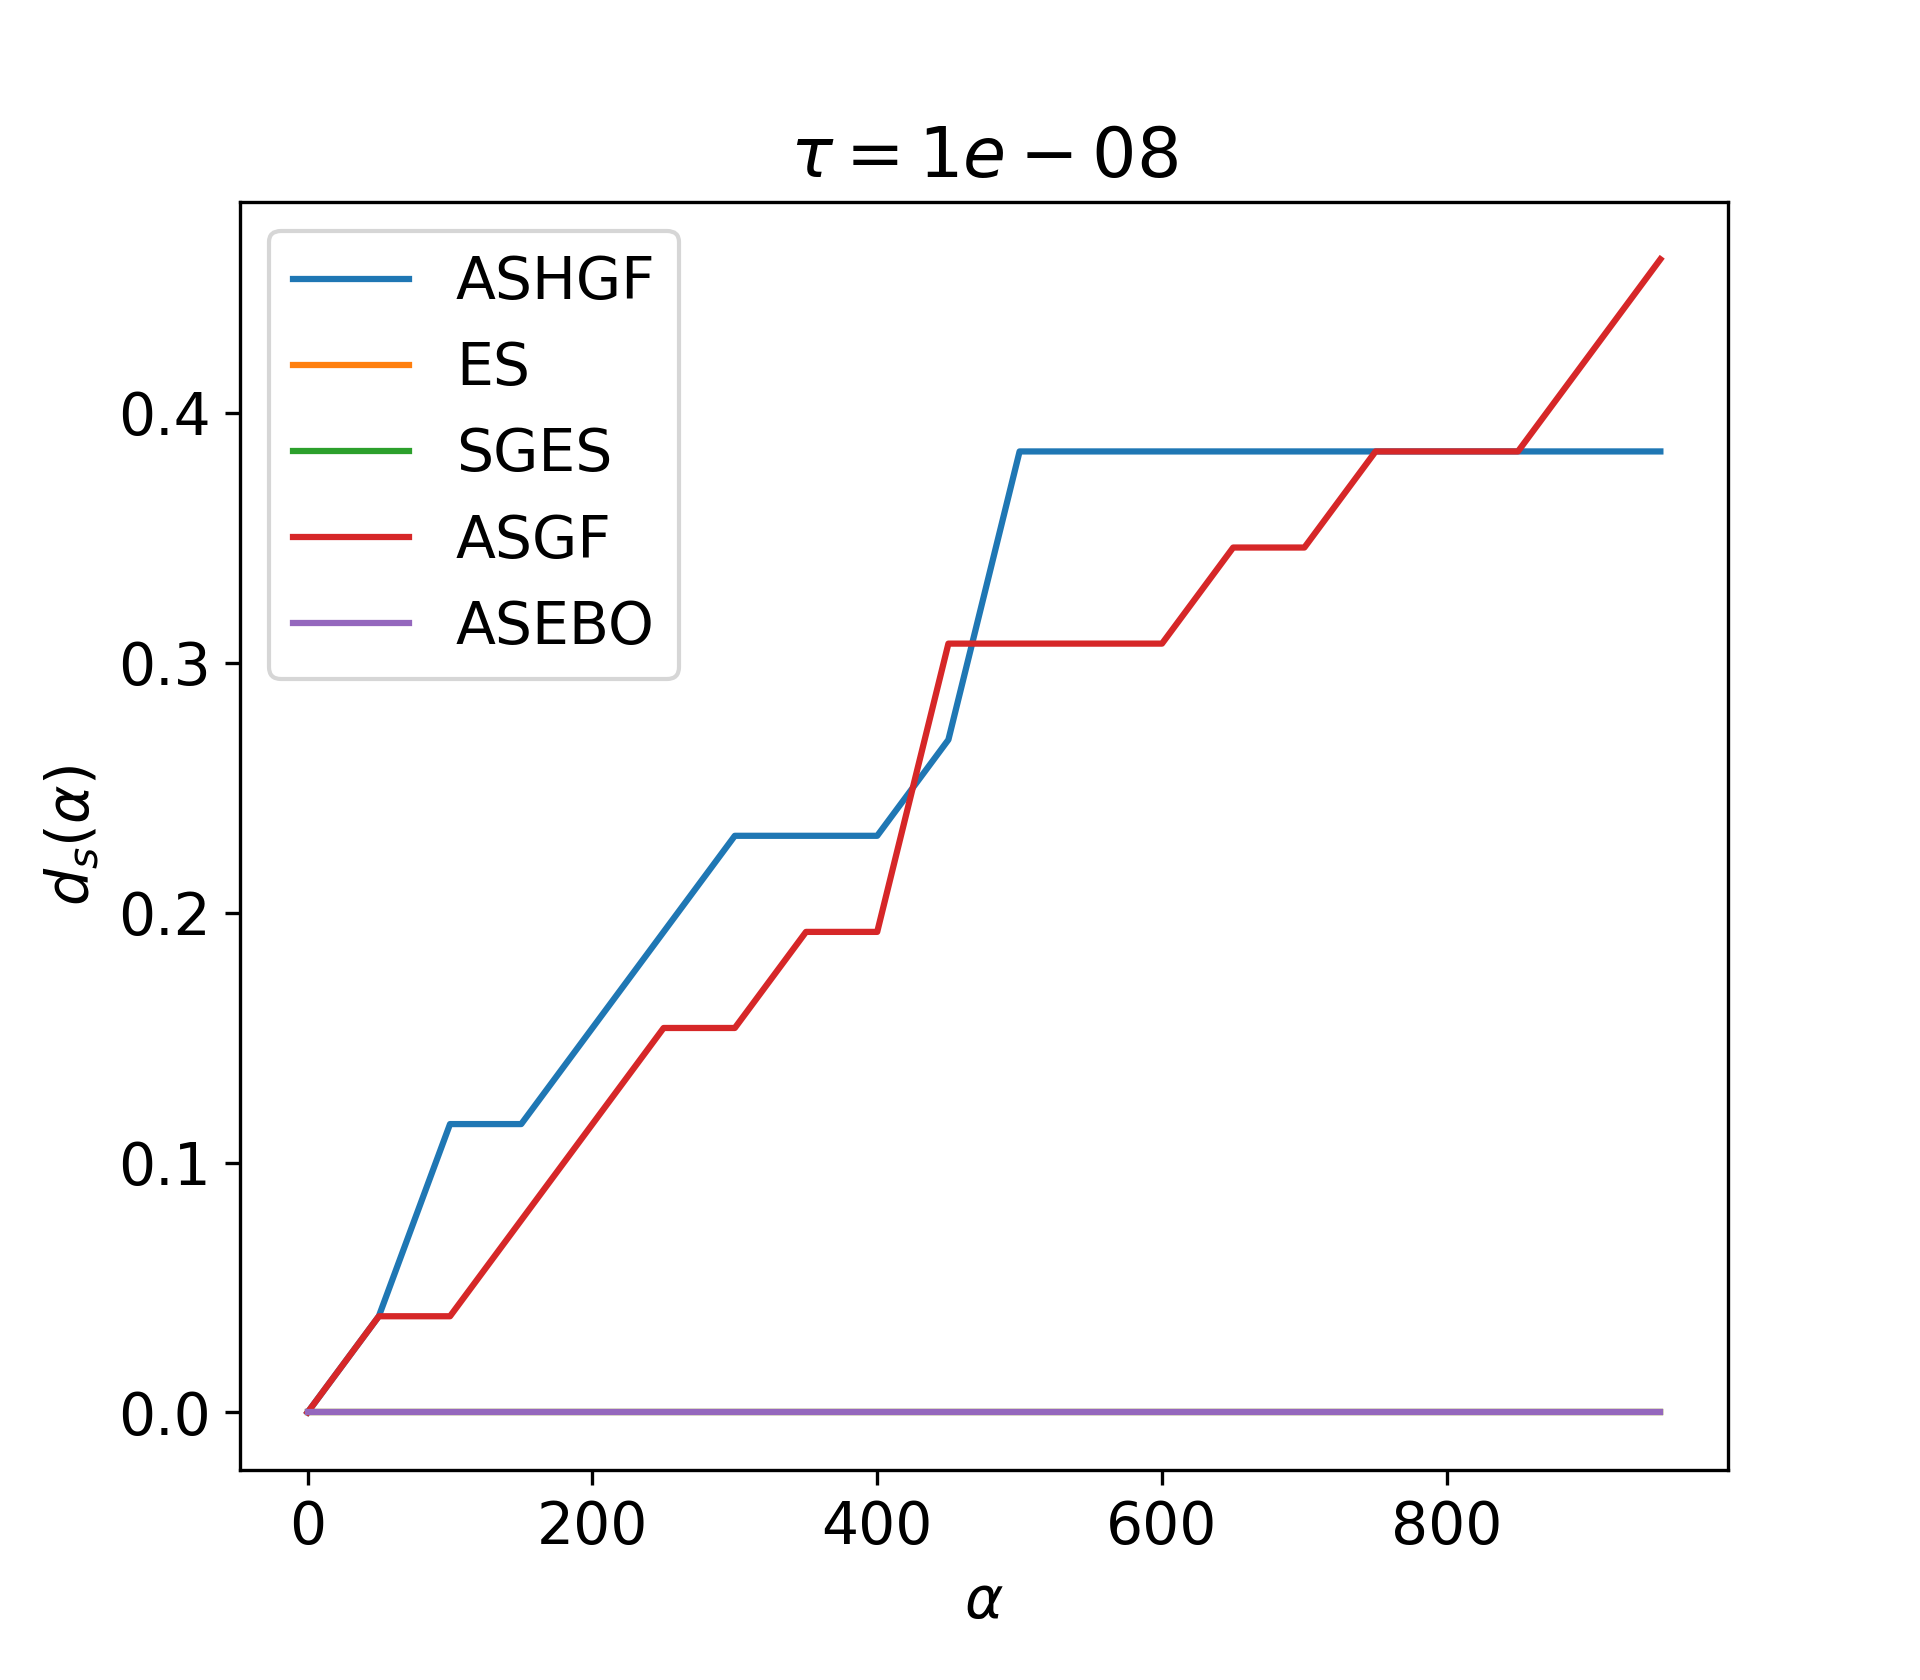
\includegraphics[width=1\textwidth]{figures/data_profiles/10/data_profile_10_1000000_1e-08.png}
\end{subfigure}%
\begin{subfigure}{0.3\textwidth}
  \centering 
  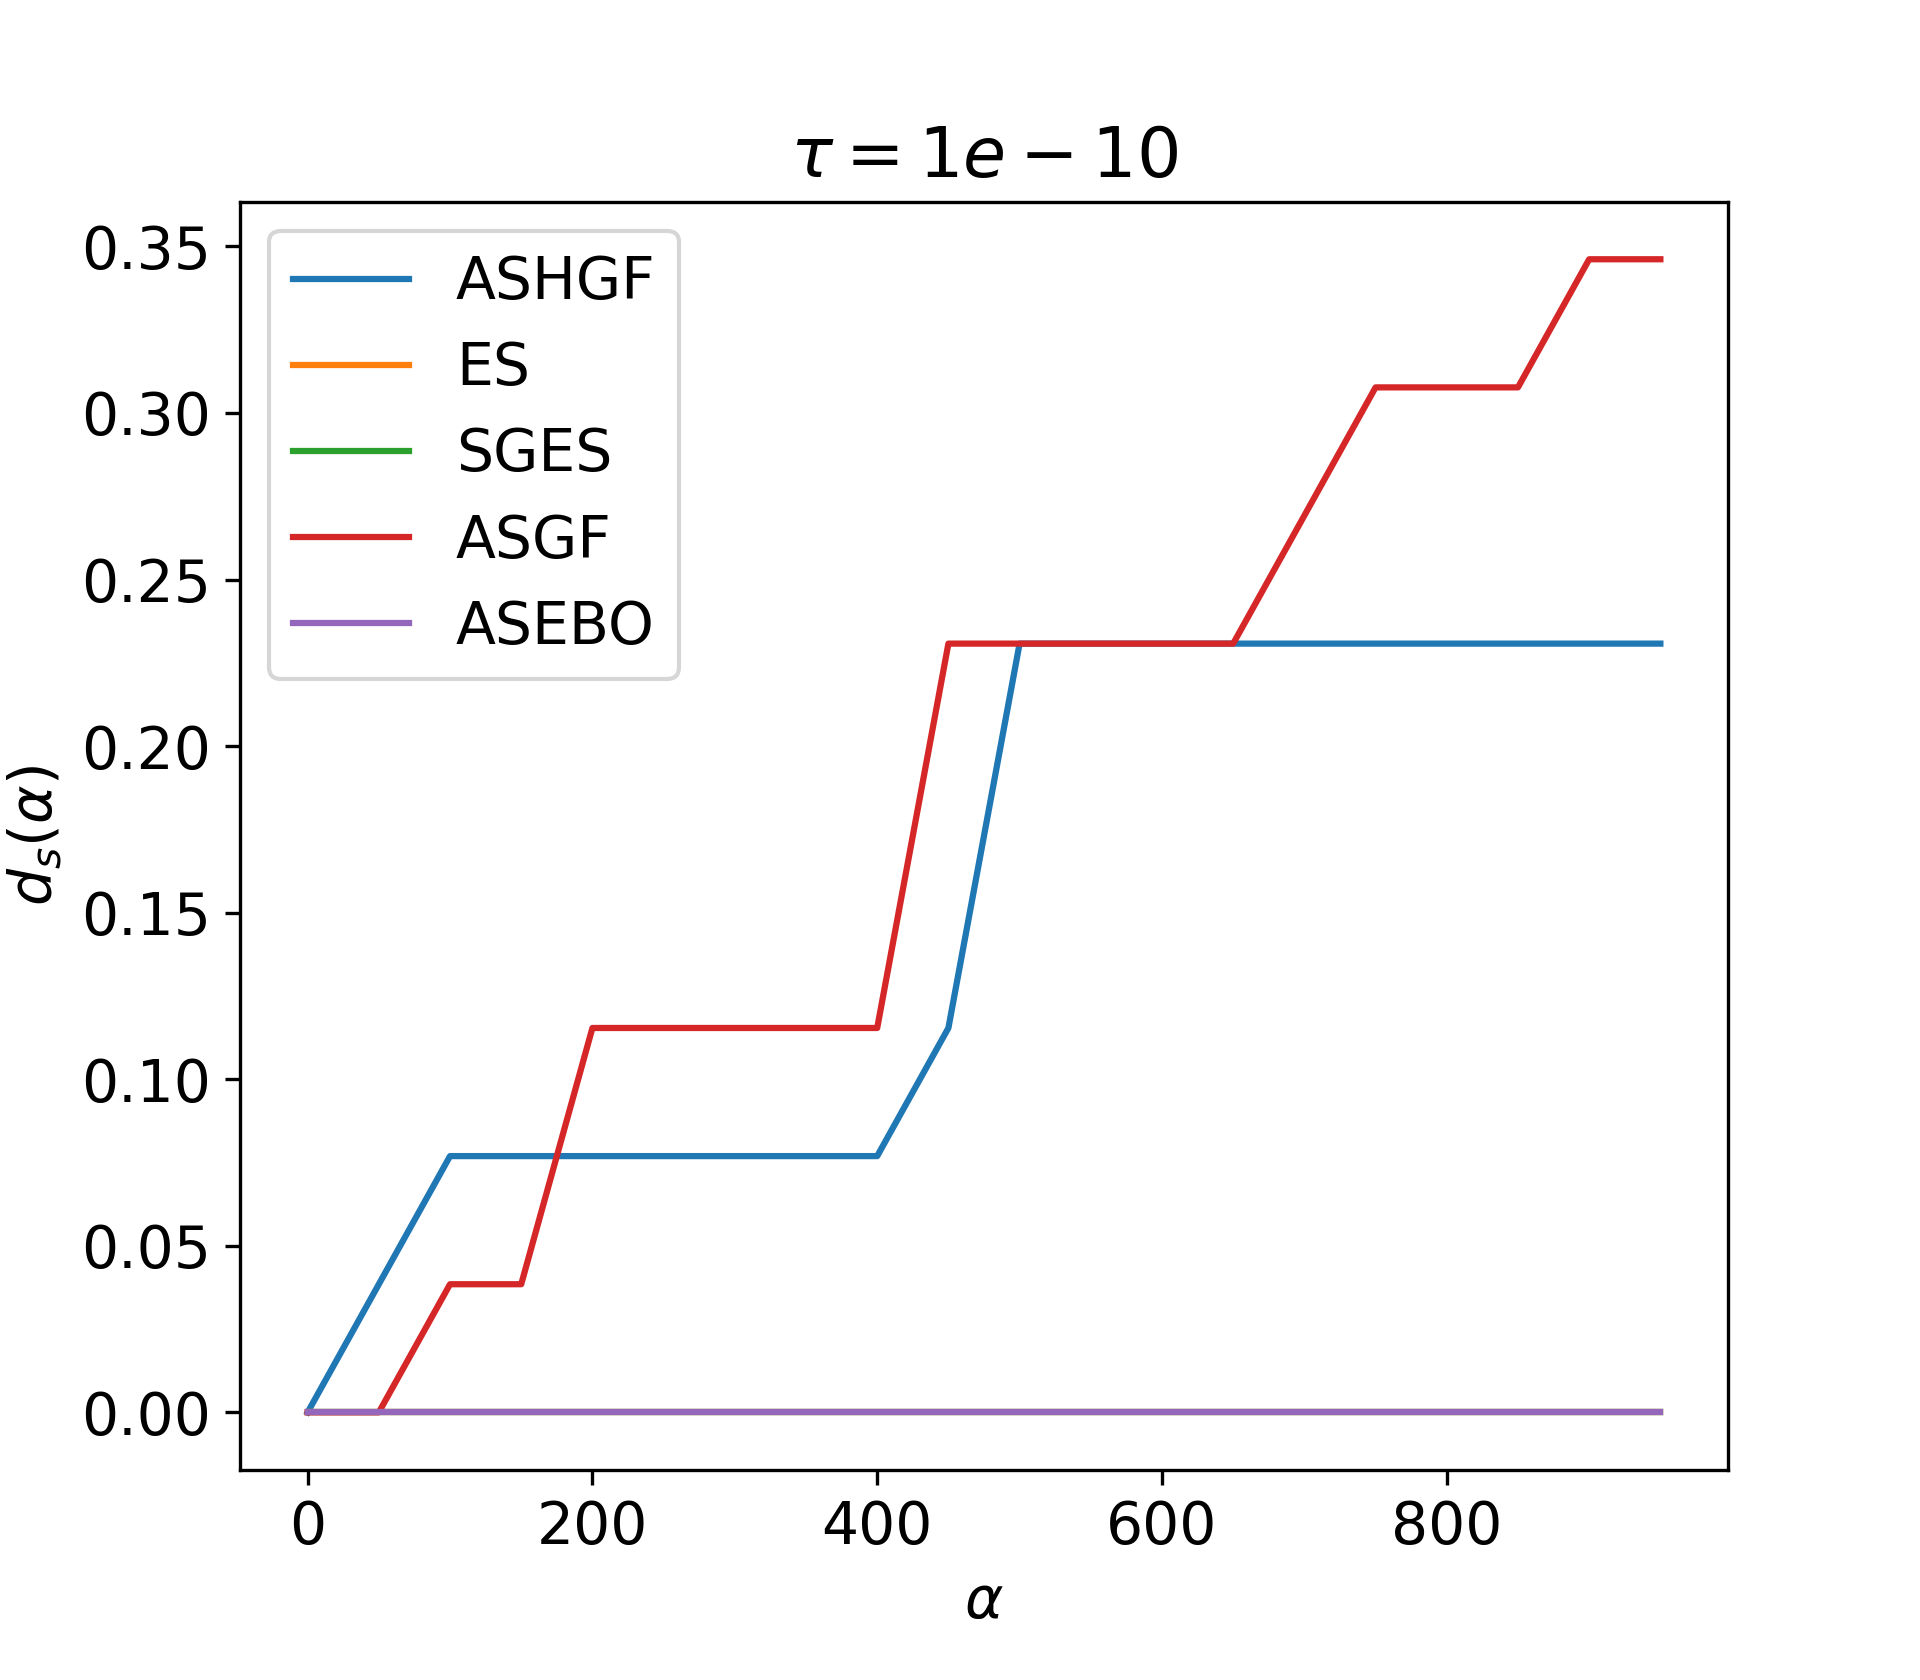
\includegraphics[width=1\textwidth]{figures/data_profiles/10/data_profile_10_1000000_1e-10.png}
\end{subfigure}
\caption{Data profiles with $\mu_L = 10^{6}$}
\label{DataProfiles10Mu1000000}
\end{figure}

\begin{figure}[H]
\centering
\begin{subfigure}{0.3\textwidth}
  \centering 
  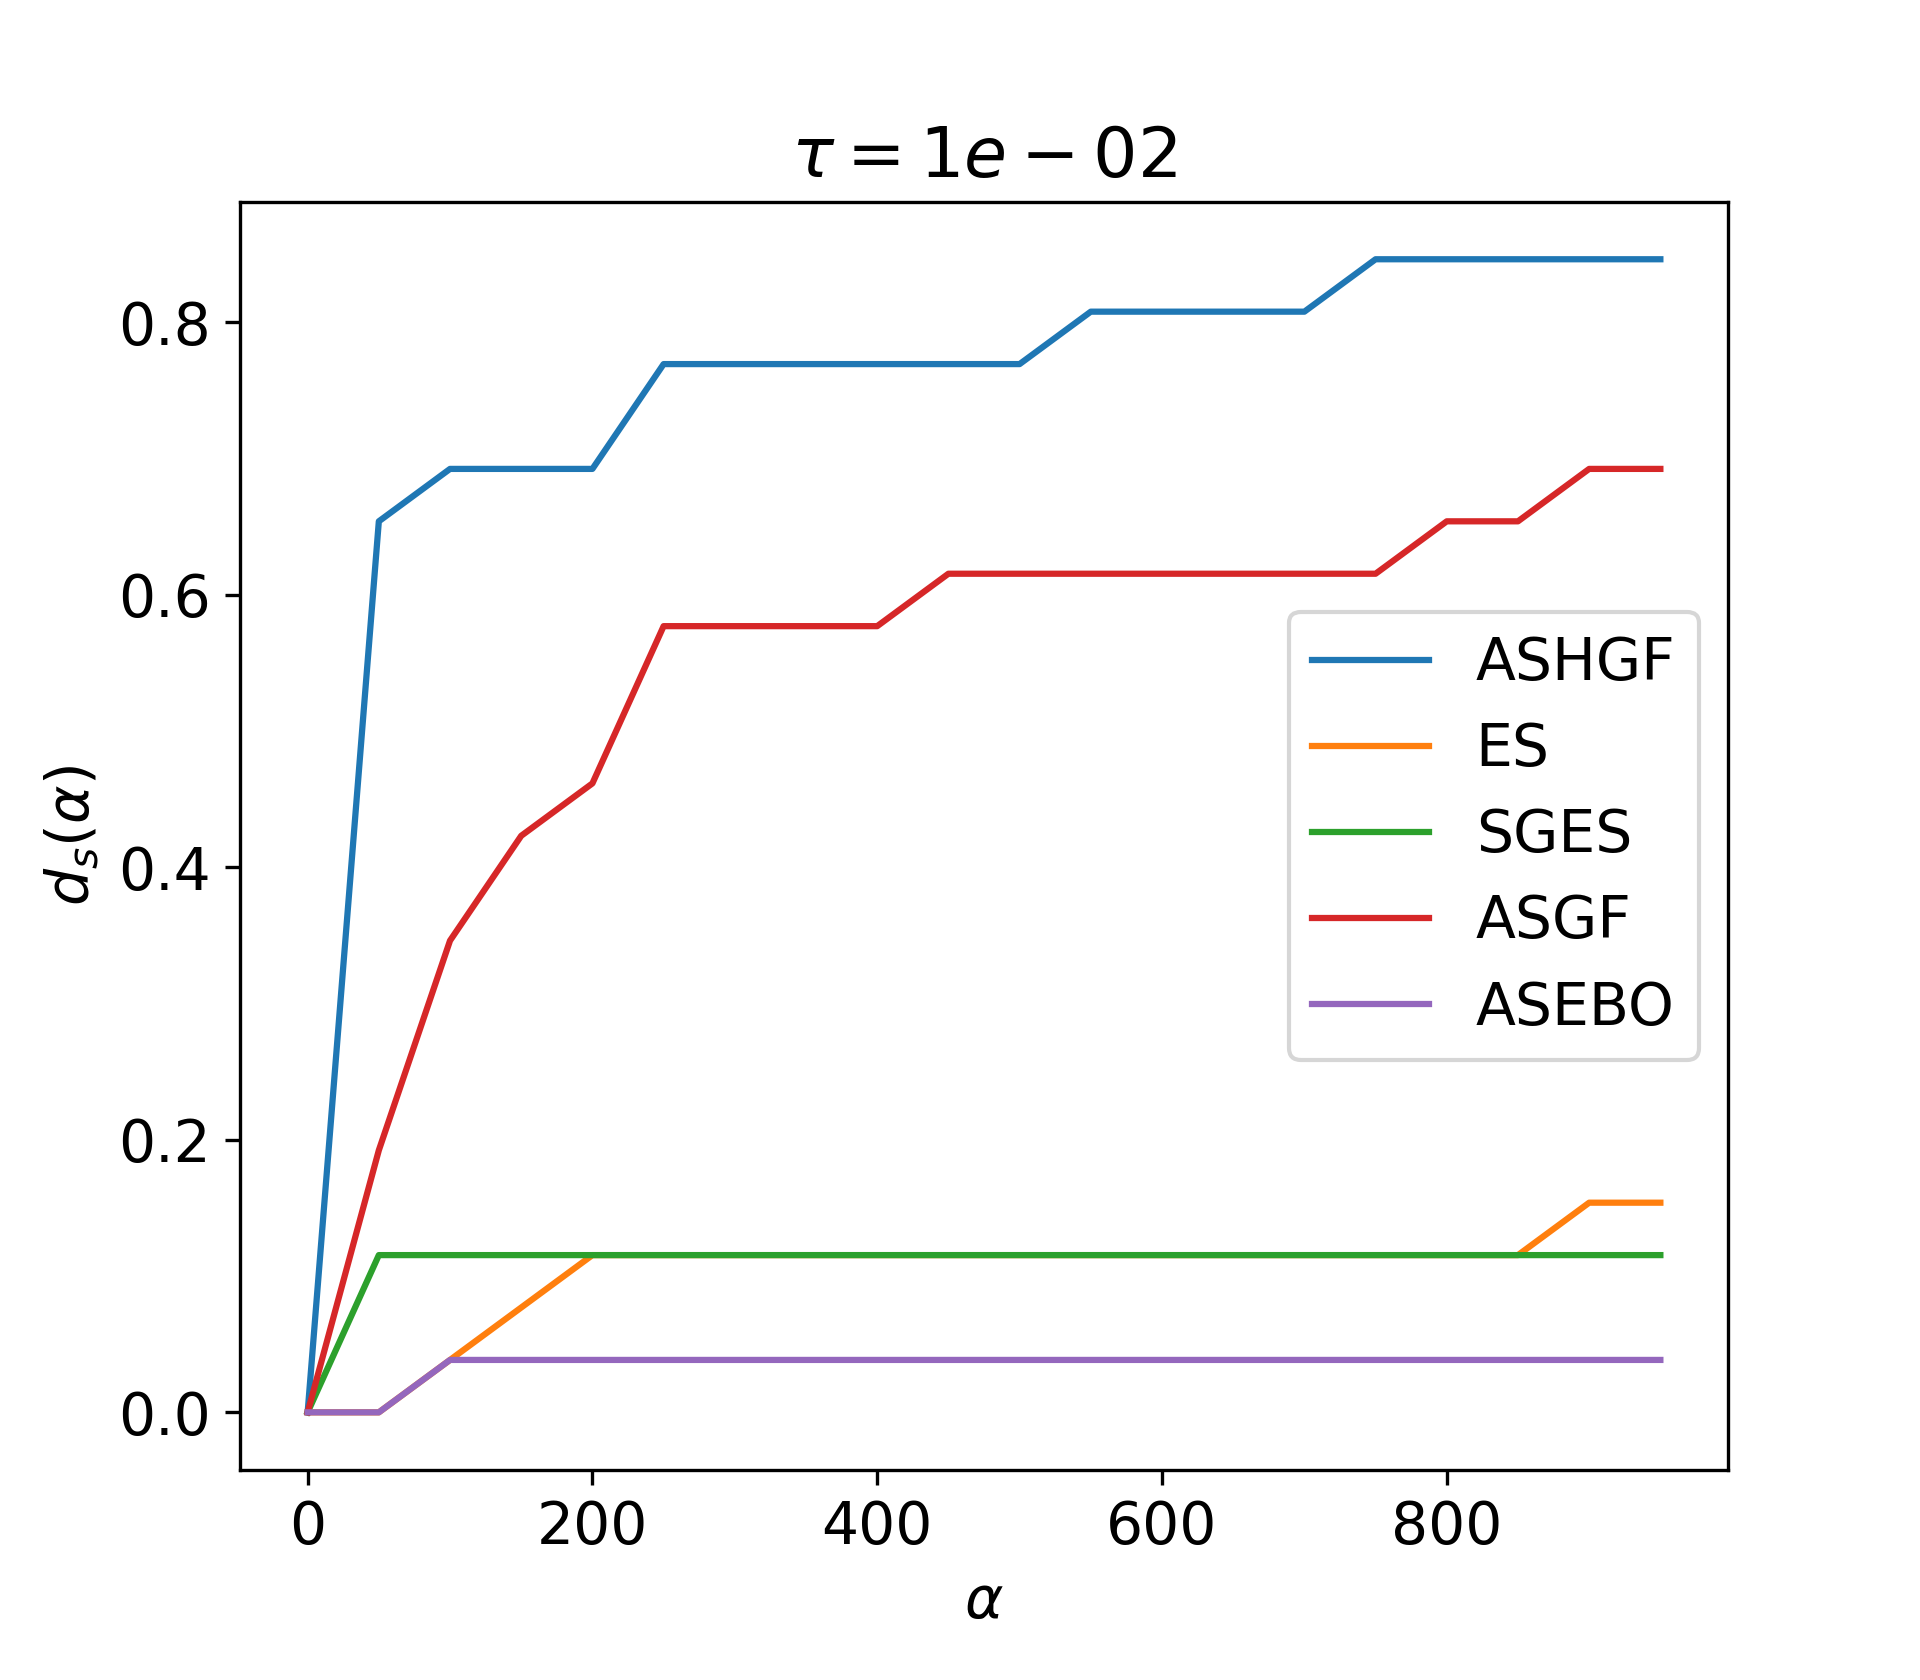
\includegraphics[width=1\textwidth]{figures/data_profiles/10/data_profile_10_10000000_1e-02.png}
\end{subfigure}%
\begin{subfigure}{0.3\textwidth}
  \centering 
  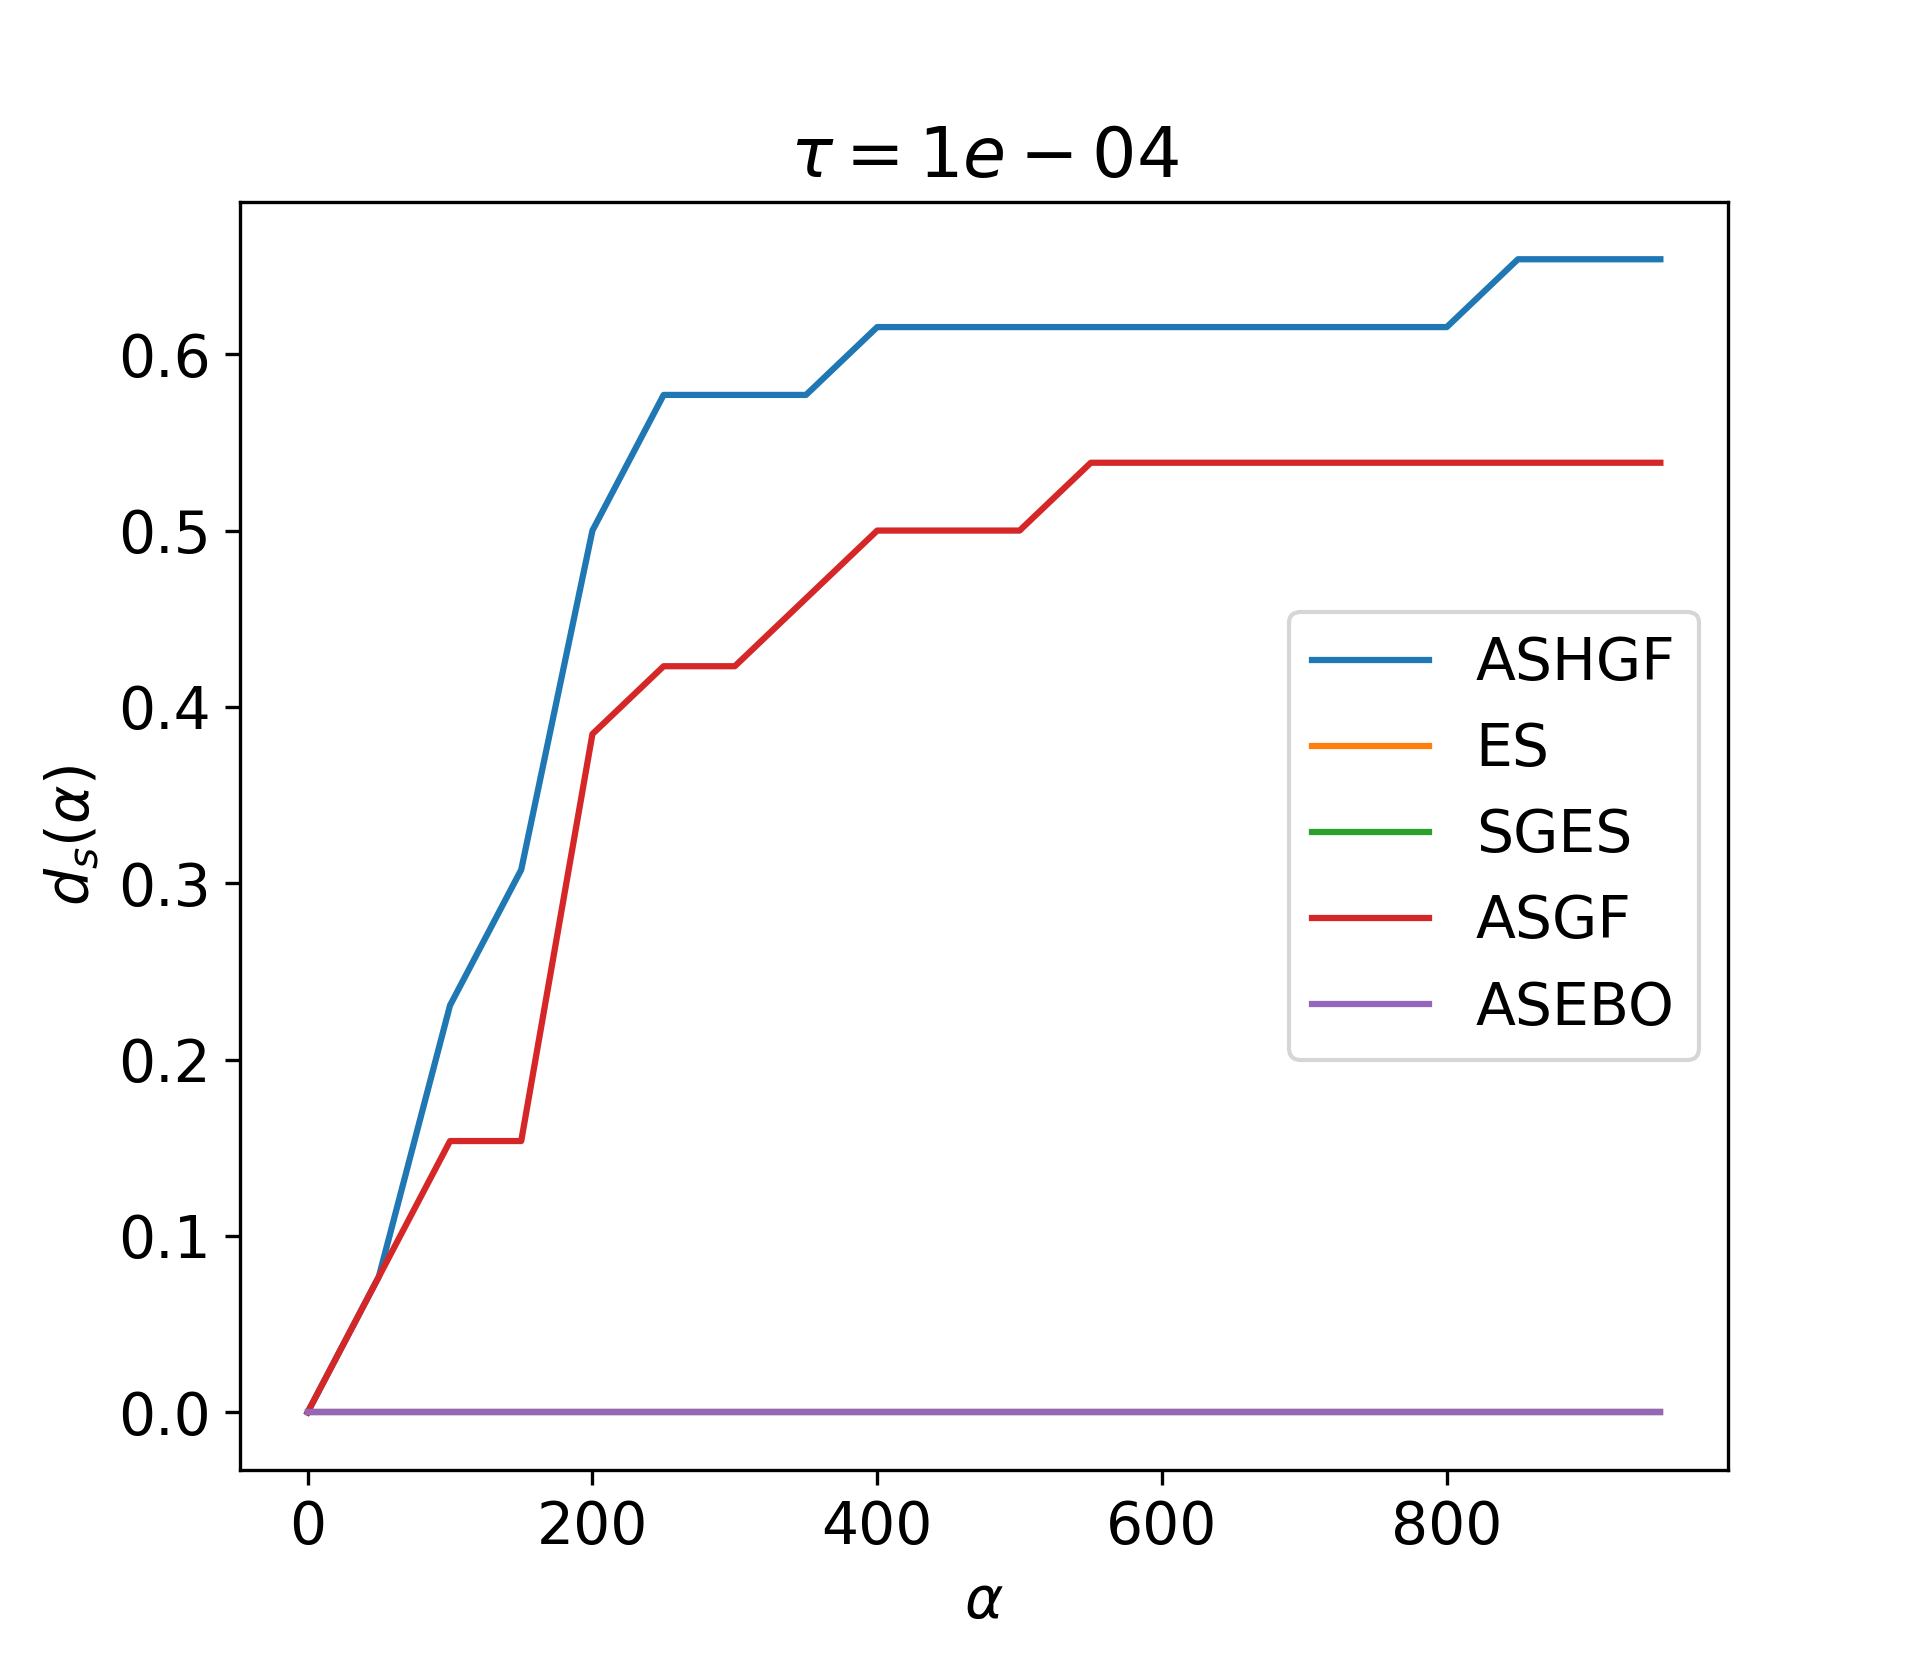
\includegraphics[width=1\textwidth]{figures/data_profiles/10/data_profile_10_10000000_1e-04.png}
\end{subfigure}
\begin{subfigure}{0.3\textwidth}
  \centering 
  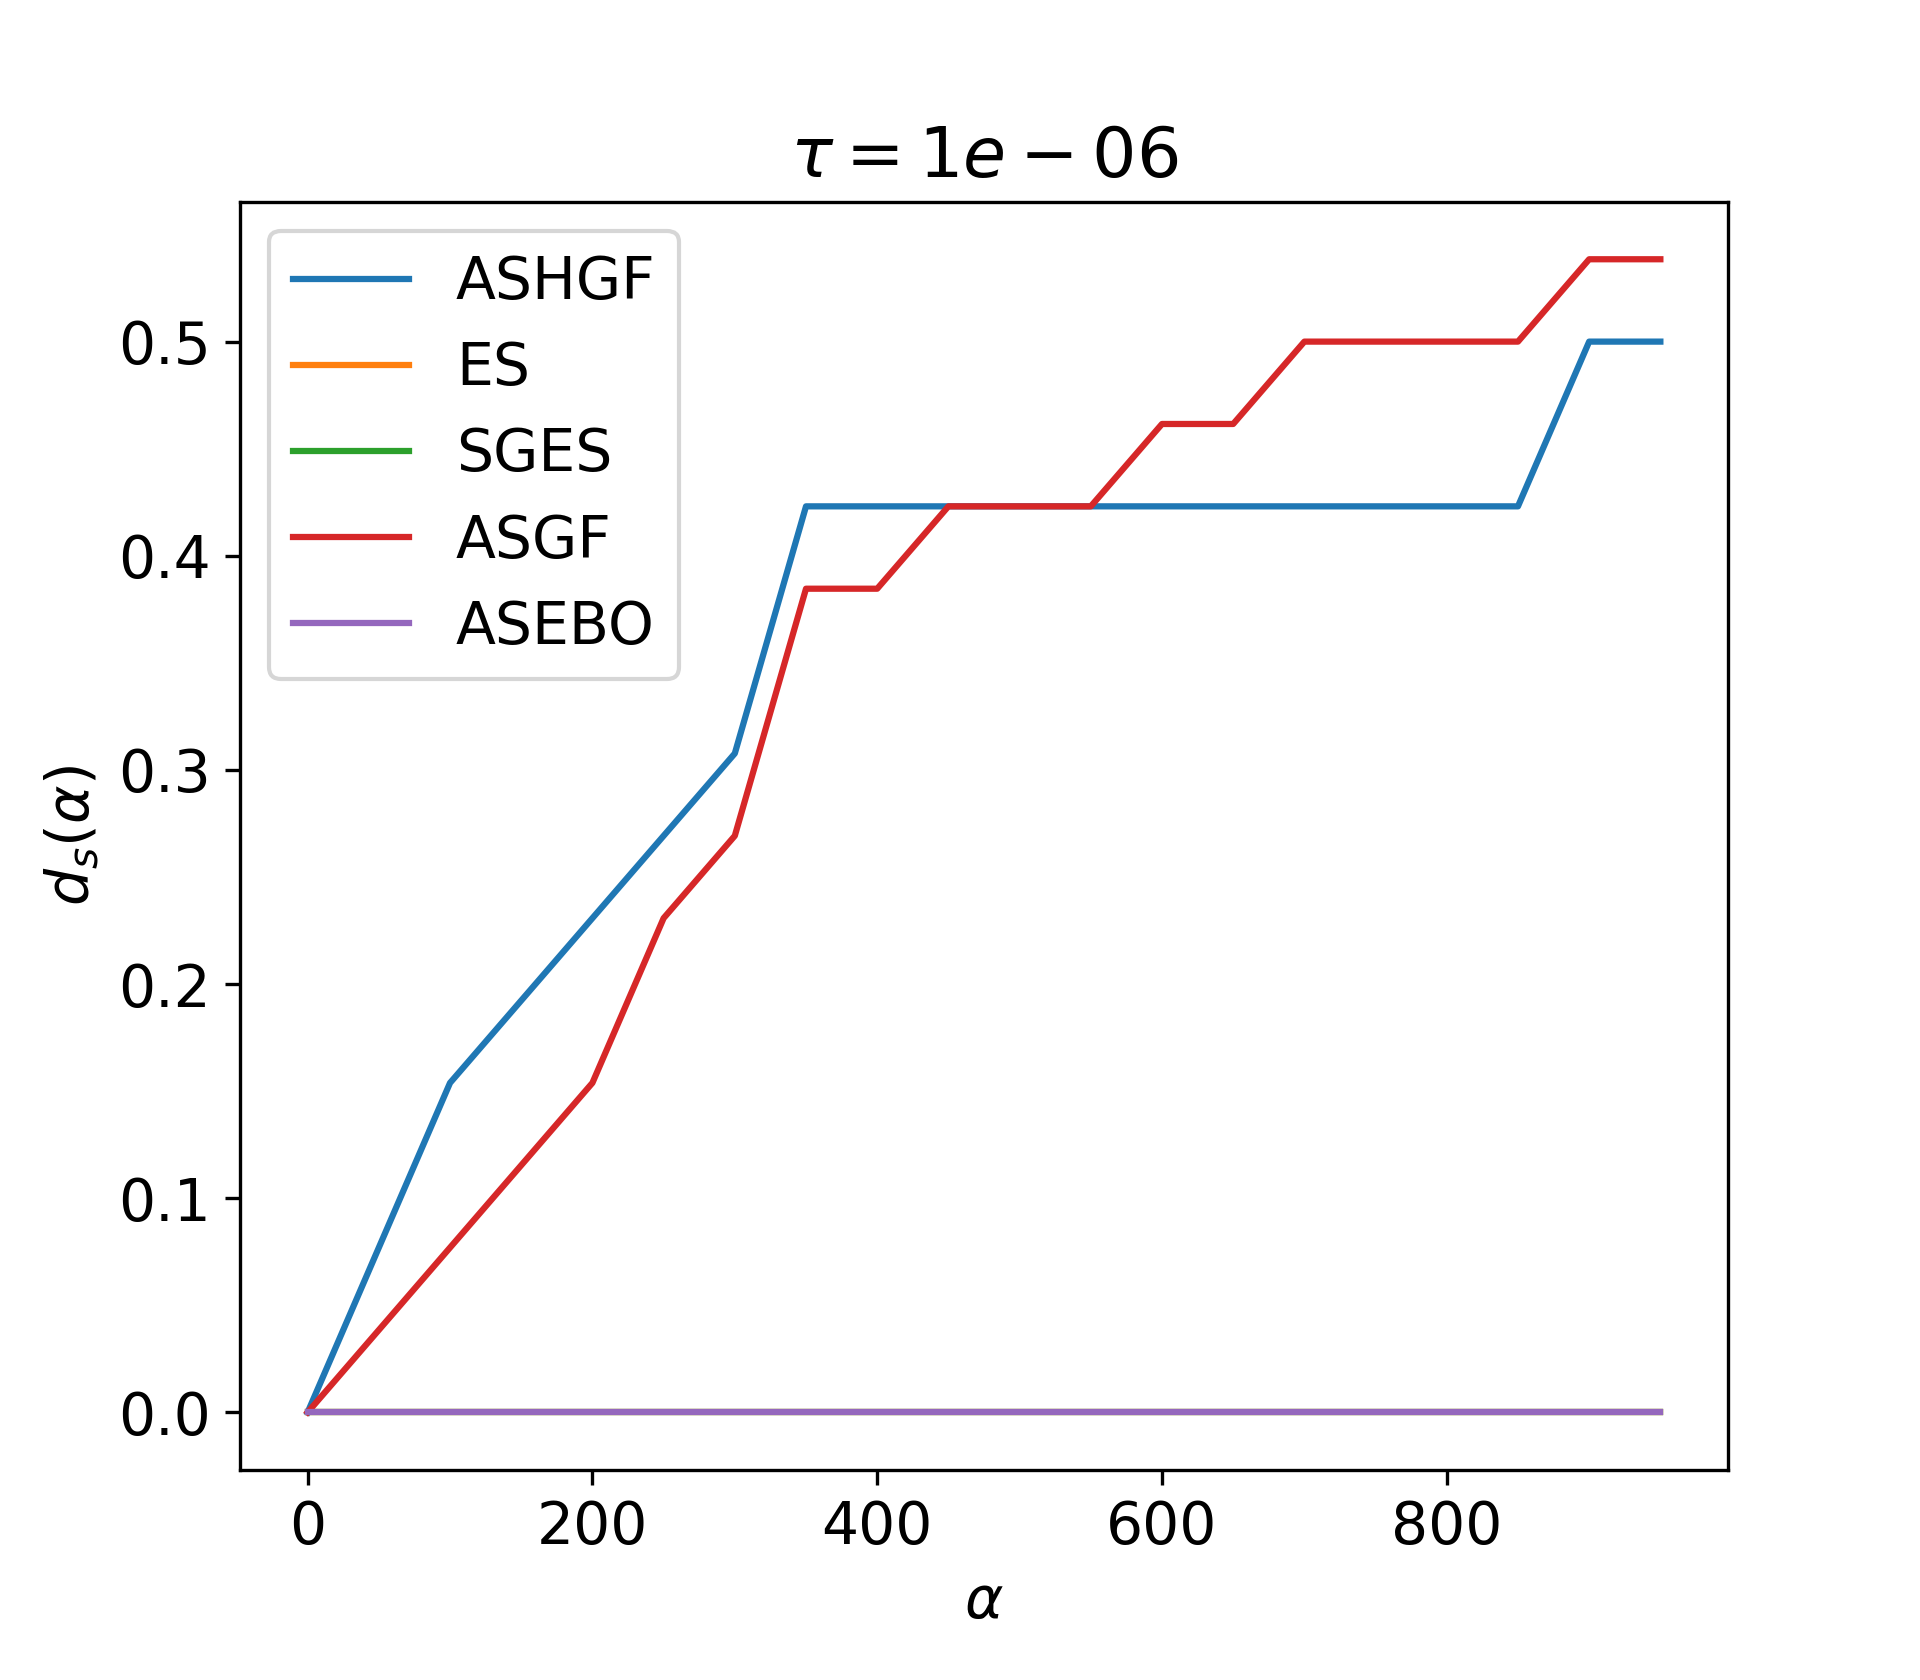
\includegraphics[width=1\textwidth]{figures/data_profiles/10/data_profile_10_10000000_1e-06.png}
\end{subfigure}
\centering
\begin{subfigure}{0.3\textwidth}
  \centering 
  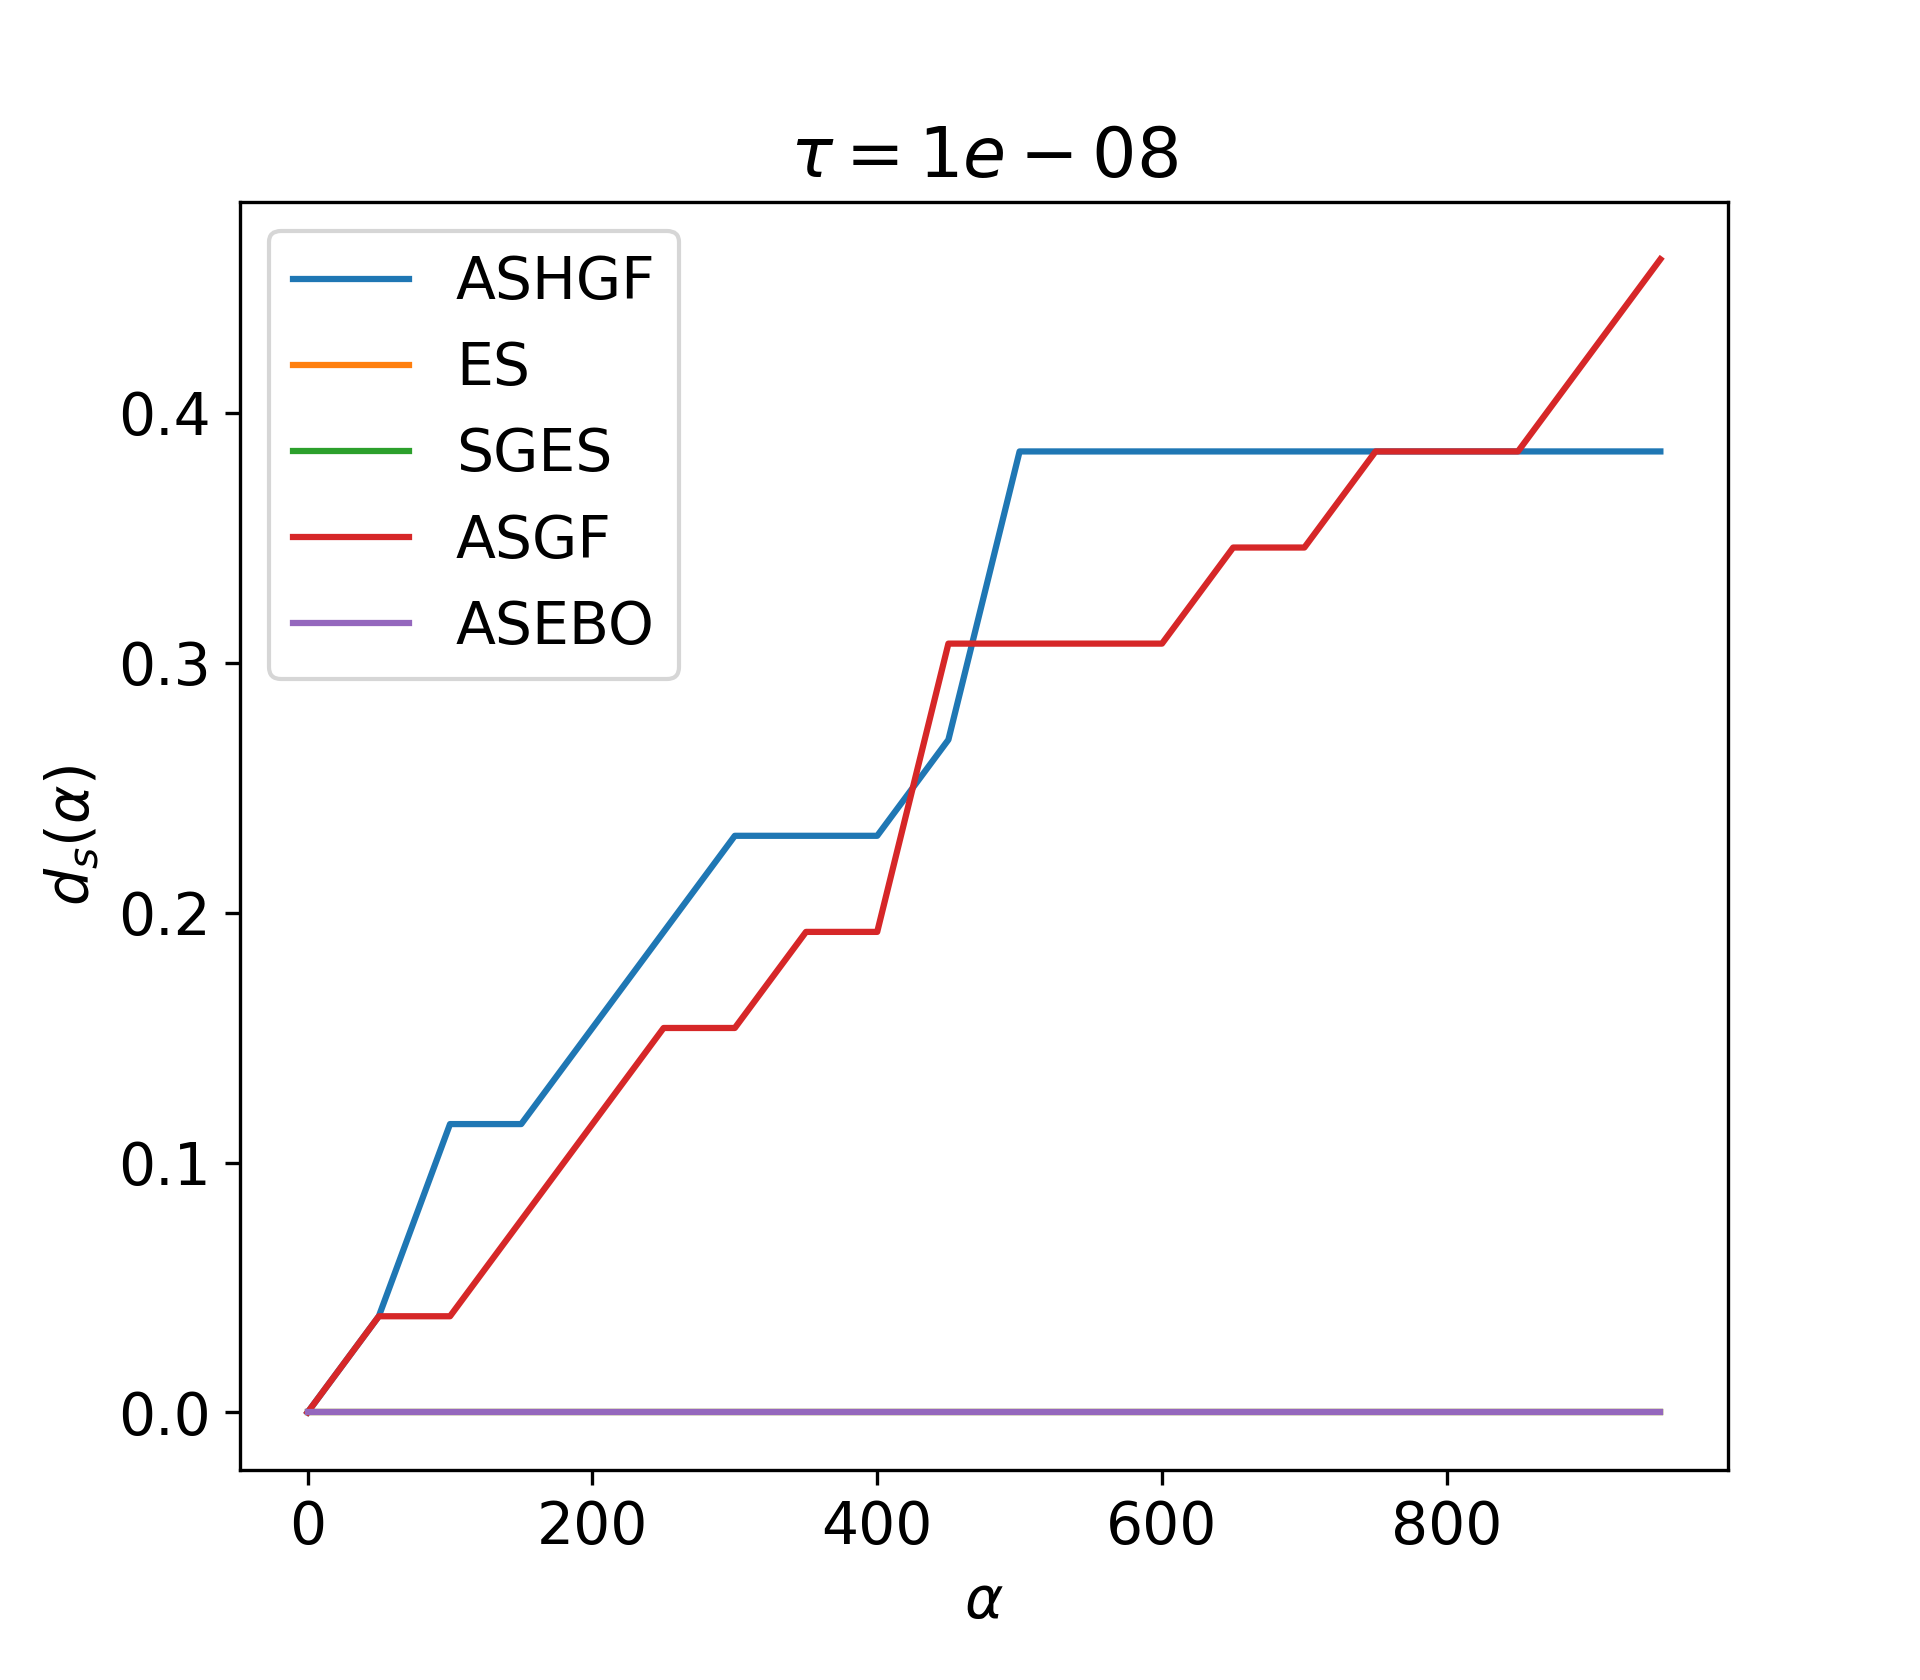
\includegraphics[width=1\textwidth]{figures/data_profiles/10/data_profile_10_10000000_1e-08.png}
\end{subfigure}%
\begin{subfigure}{0.3\textwidth}
  \centering 
  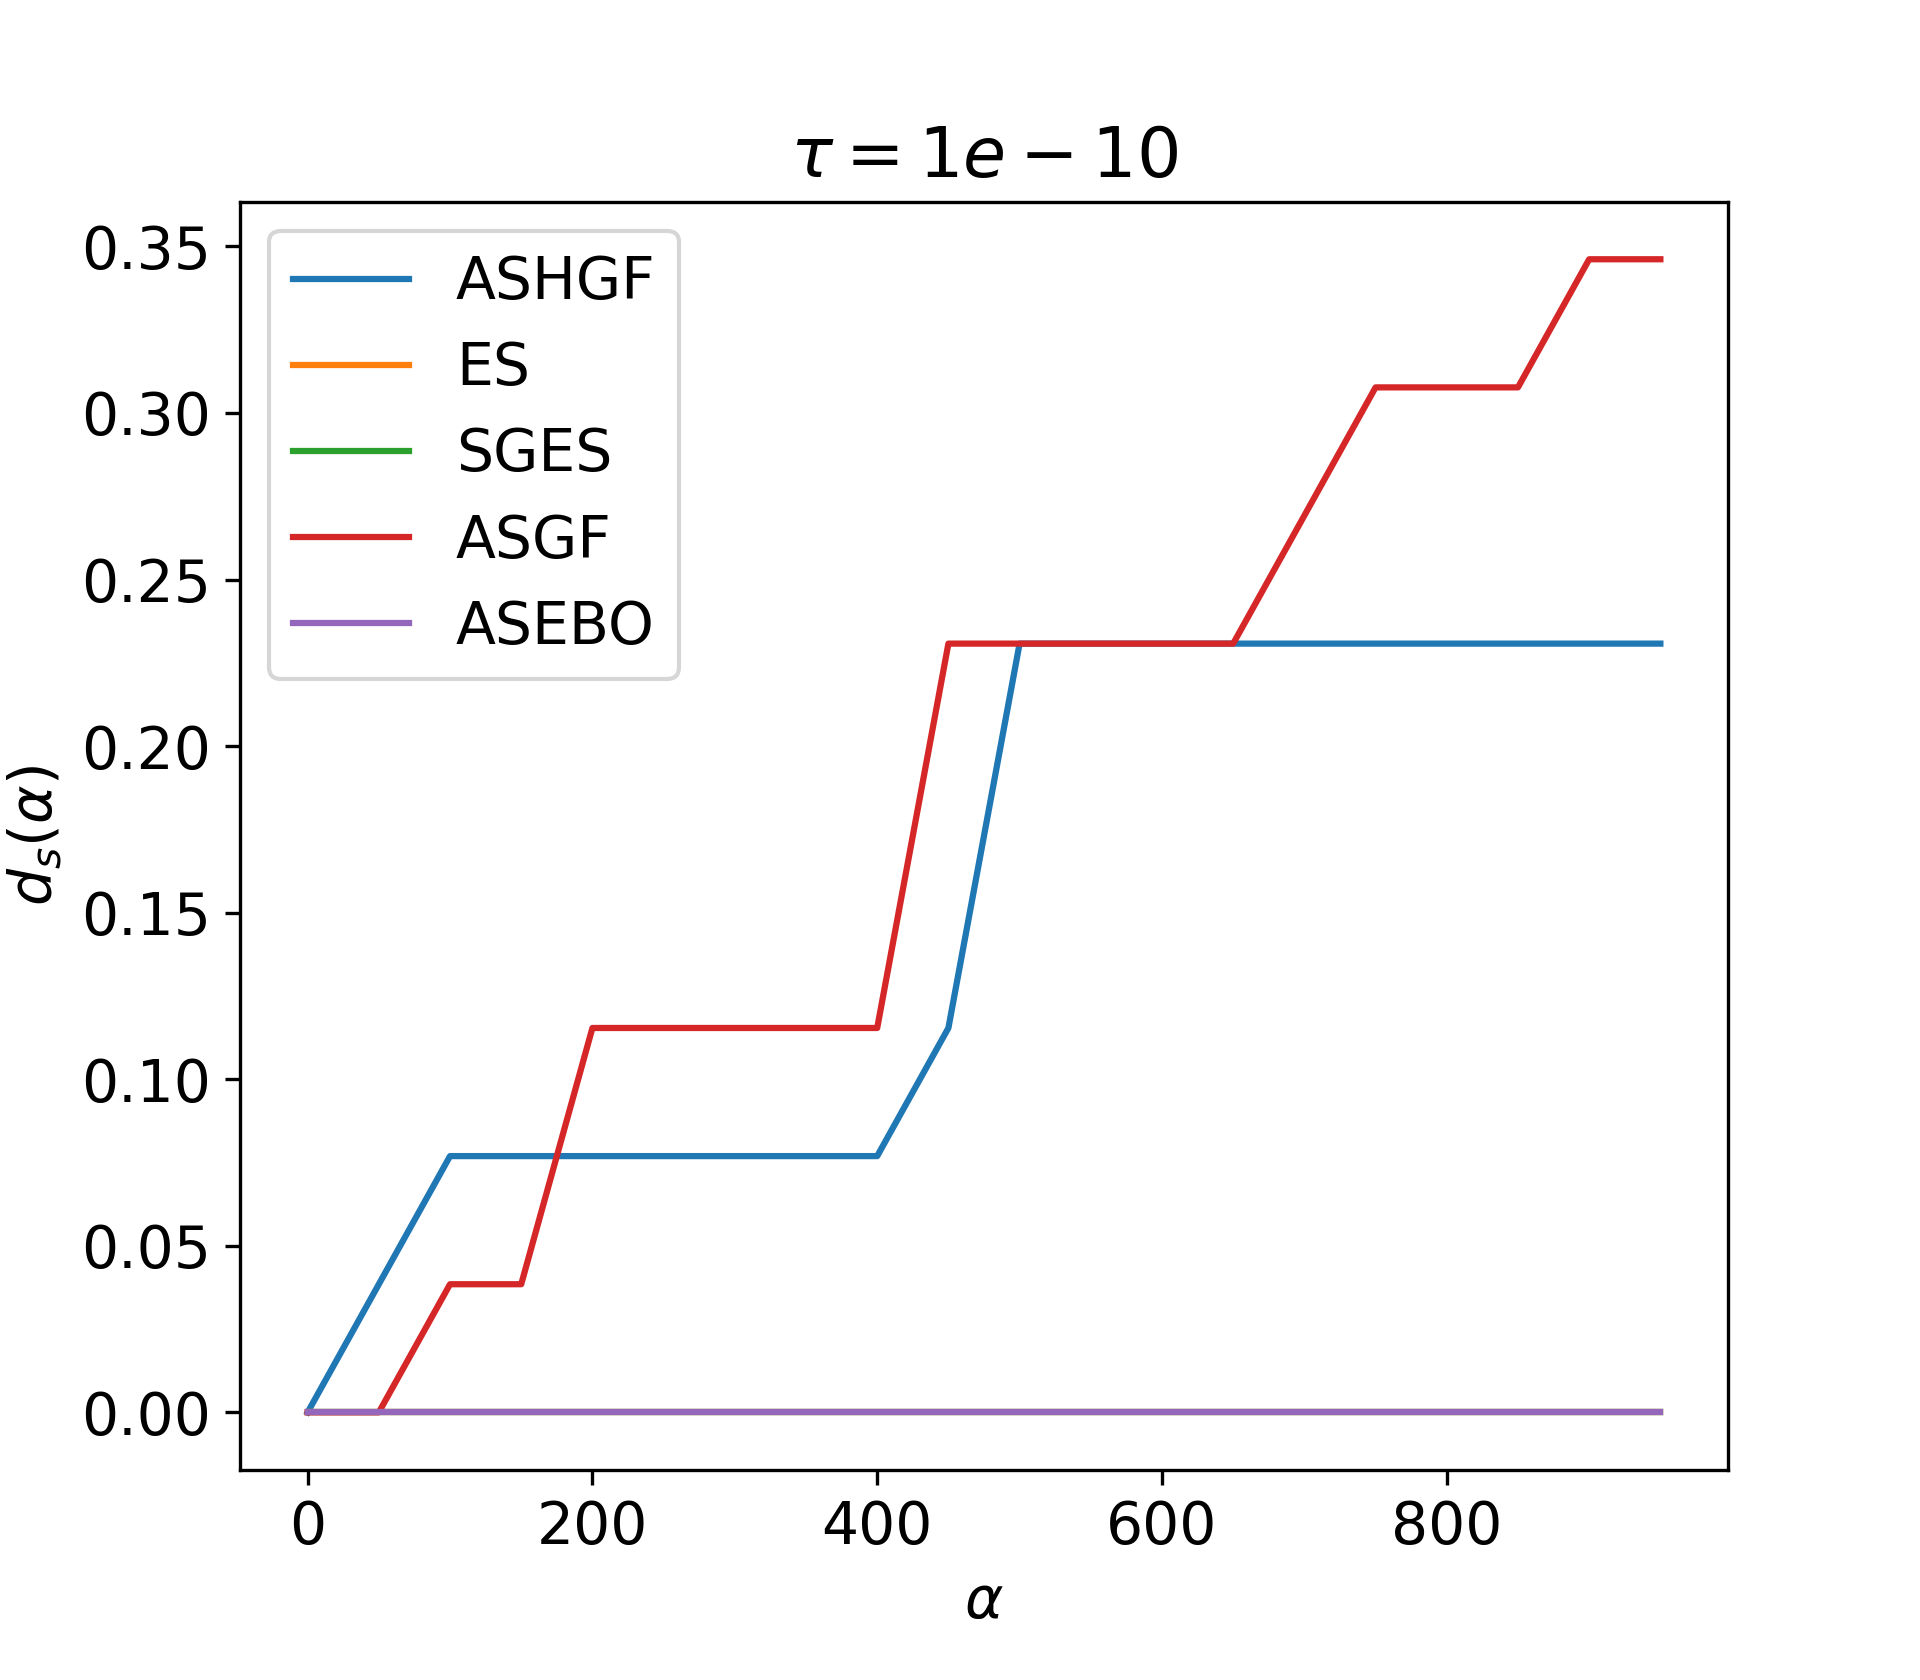
\includegraphics[width=1\textwidth]{figures/data_profiles/10/data_profile_10_10000000_1e-10.png}
\end{subfigure}
\caption{Data profiles with $\mu_L = 10^{7}$}
\label{DataProfiles10Mu10000000}
\end{figure}

\begin{figure}[H]
	\centering
	\begin{subfigure}{0.3\textwidth}
		\centering 
		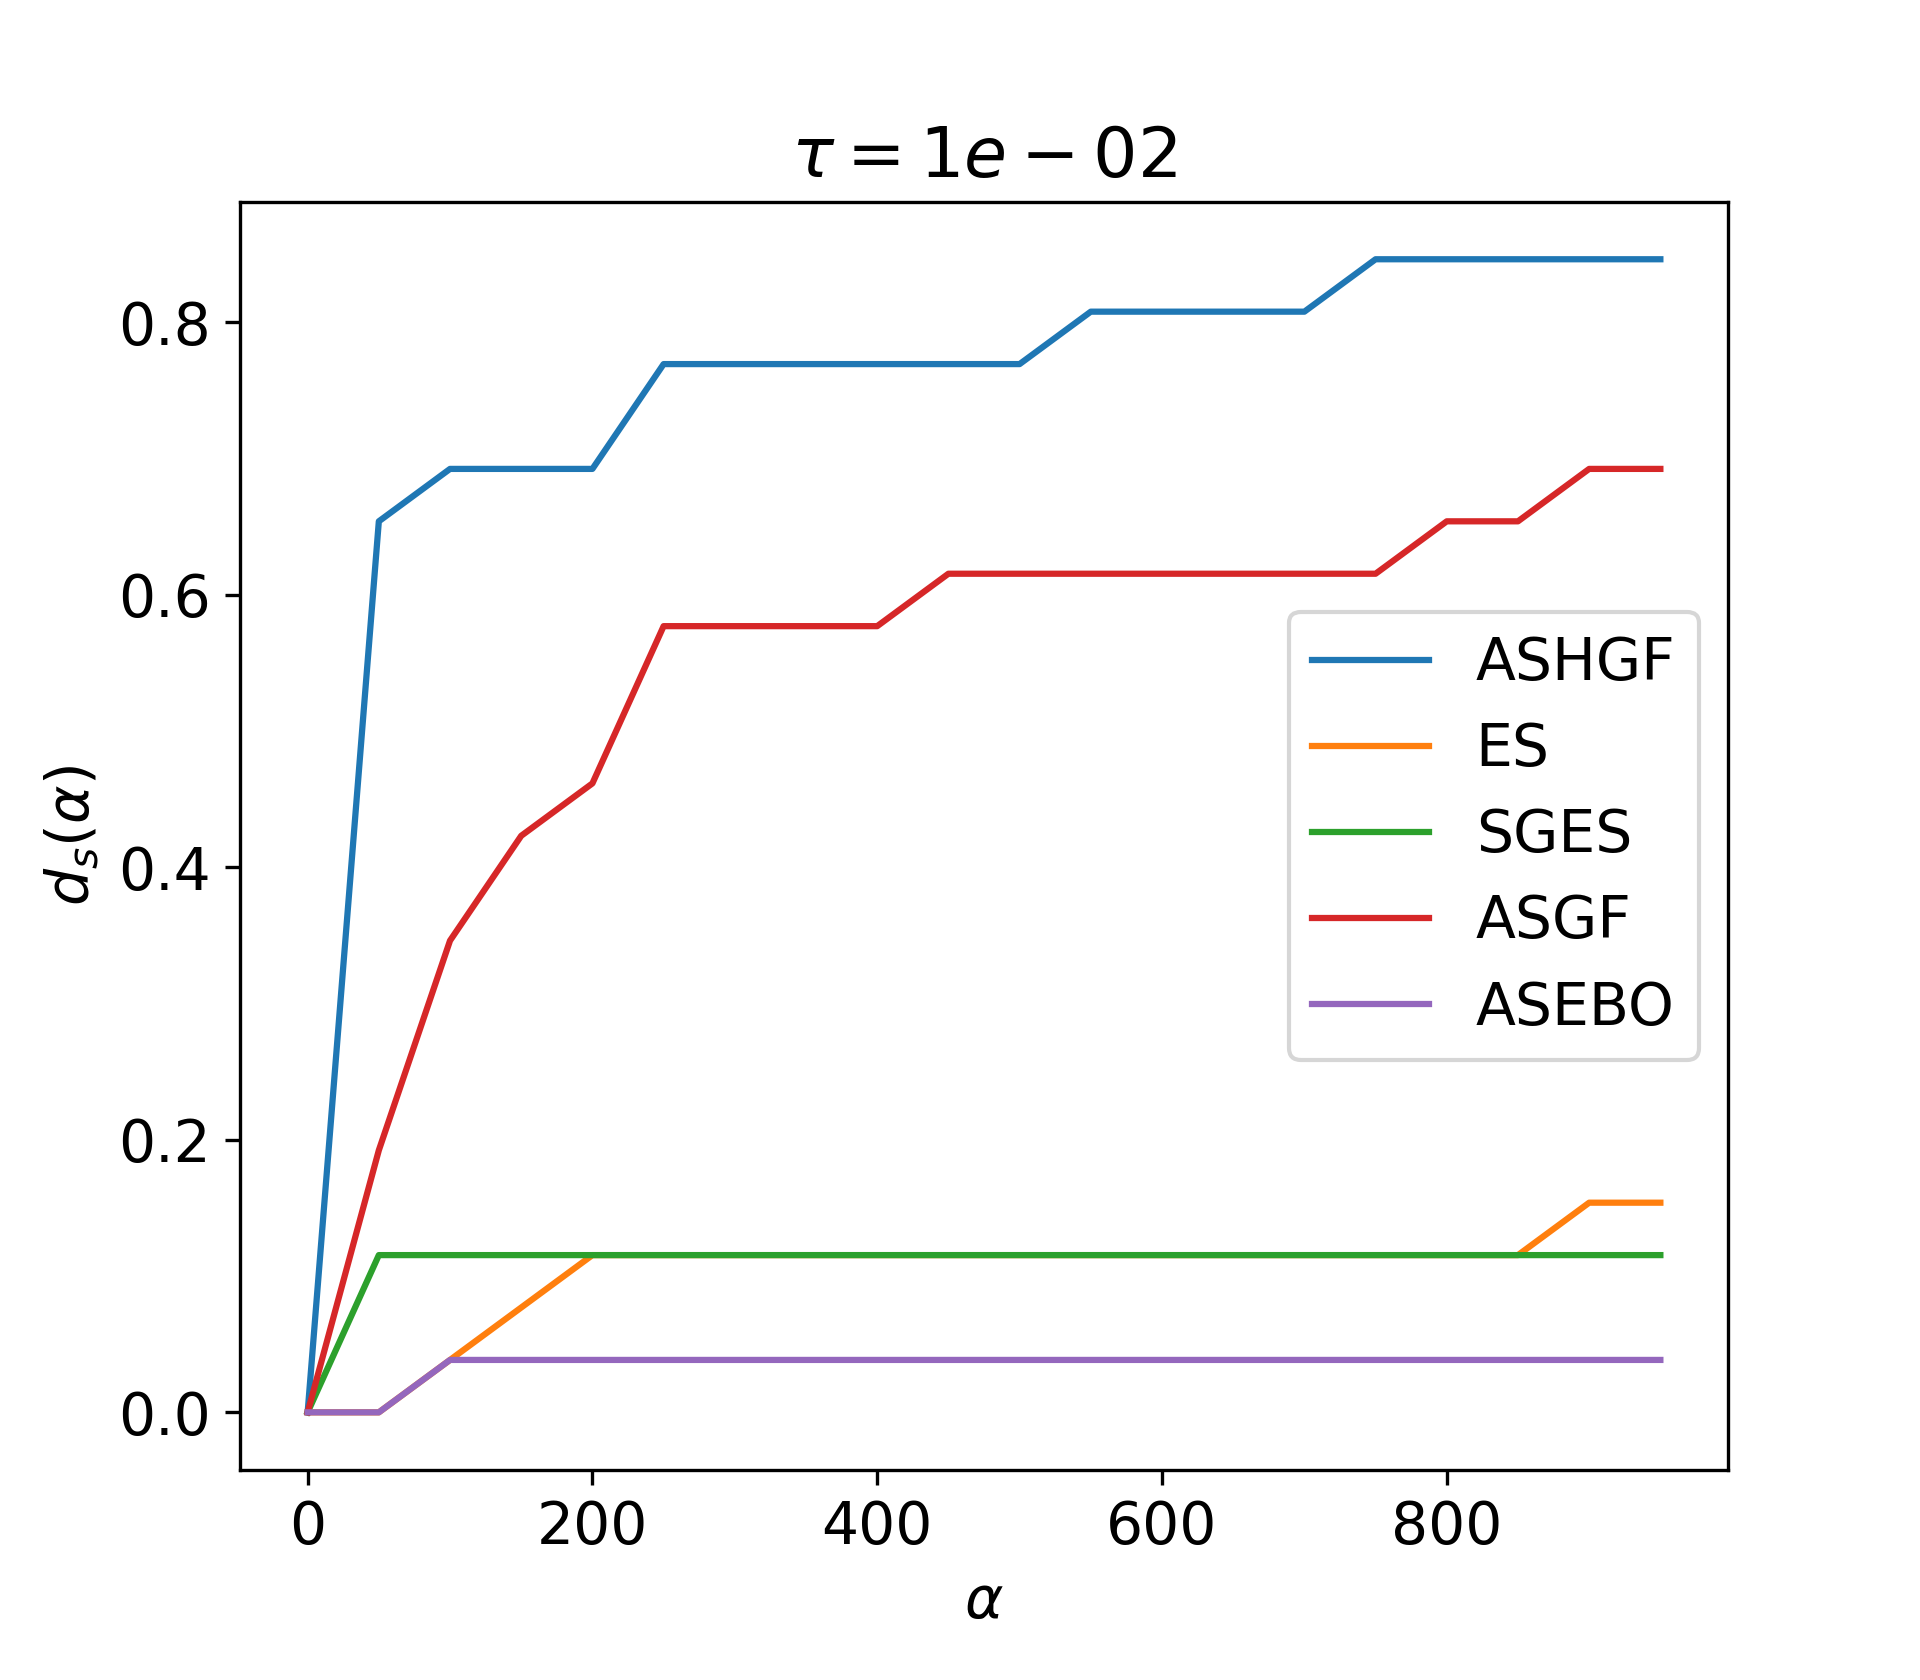
\includegraphics[width=1\textwidth]{figures/data_profiles/10/data_profile_10_100000000_1e-02.png}
	\end{subfigure}%
	\begin{subfigure}{0.3\textwidth}
		\centering 
		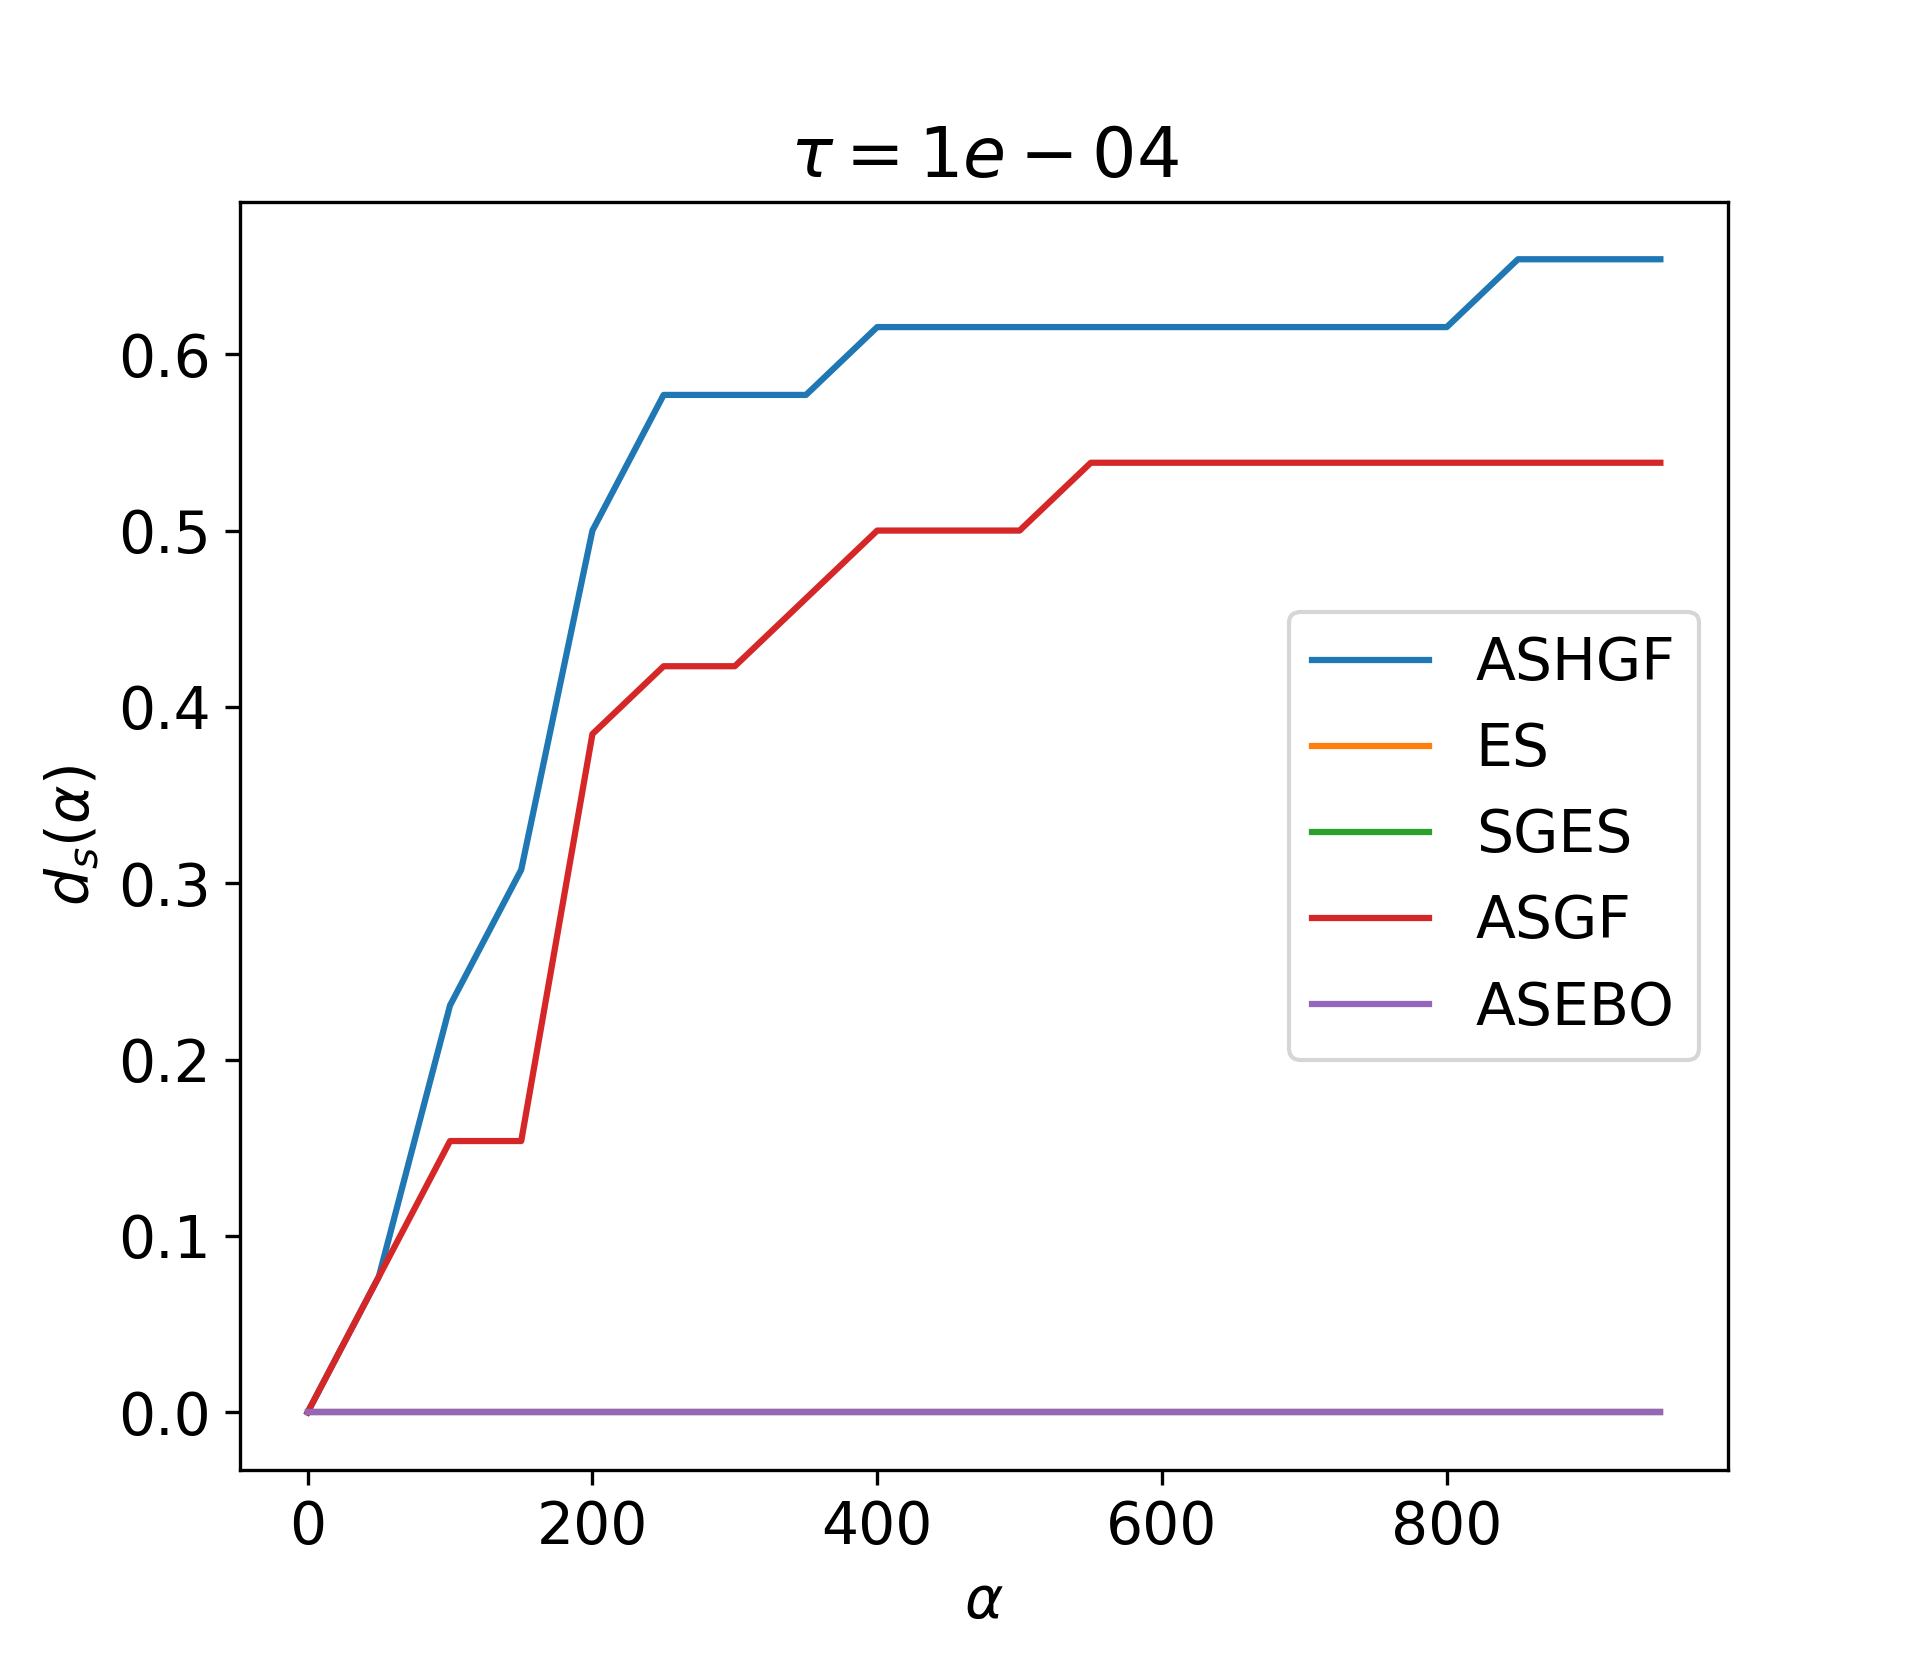
\includegraphics[width=1\textwidth]{figures/data_profiles/10/data_profile_10_100000000_1e-04.png}
	\end{subfigure}
	\begin{subfigure}{0.3\textwidth}
		\centering 
		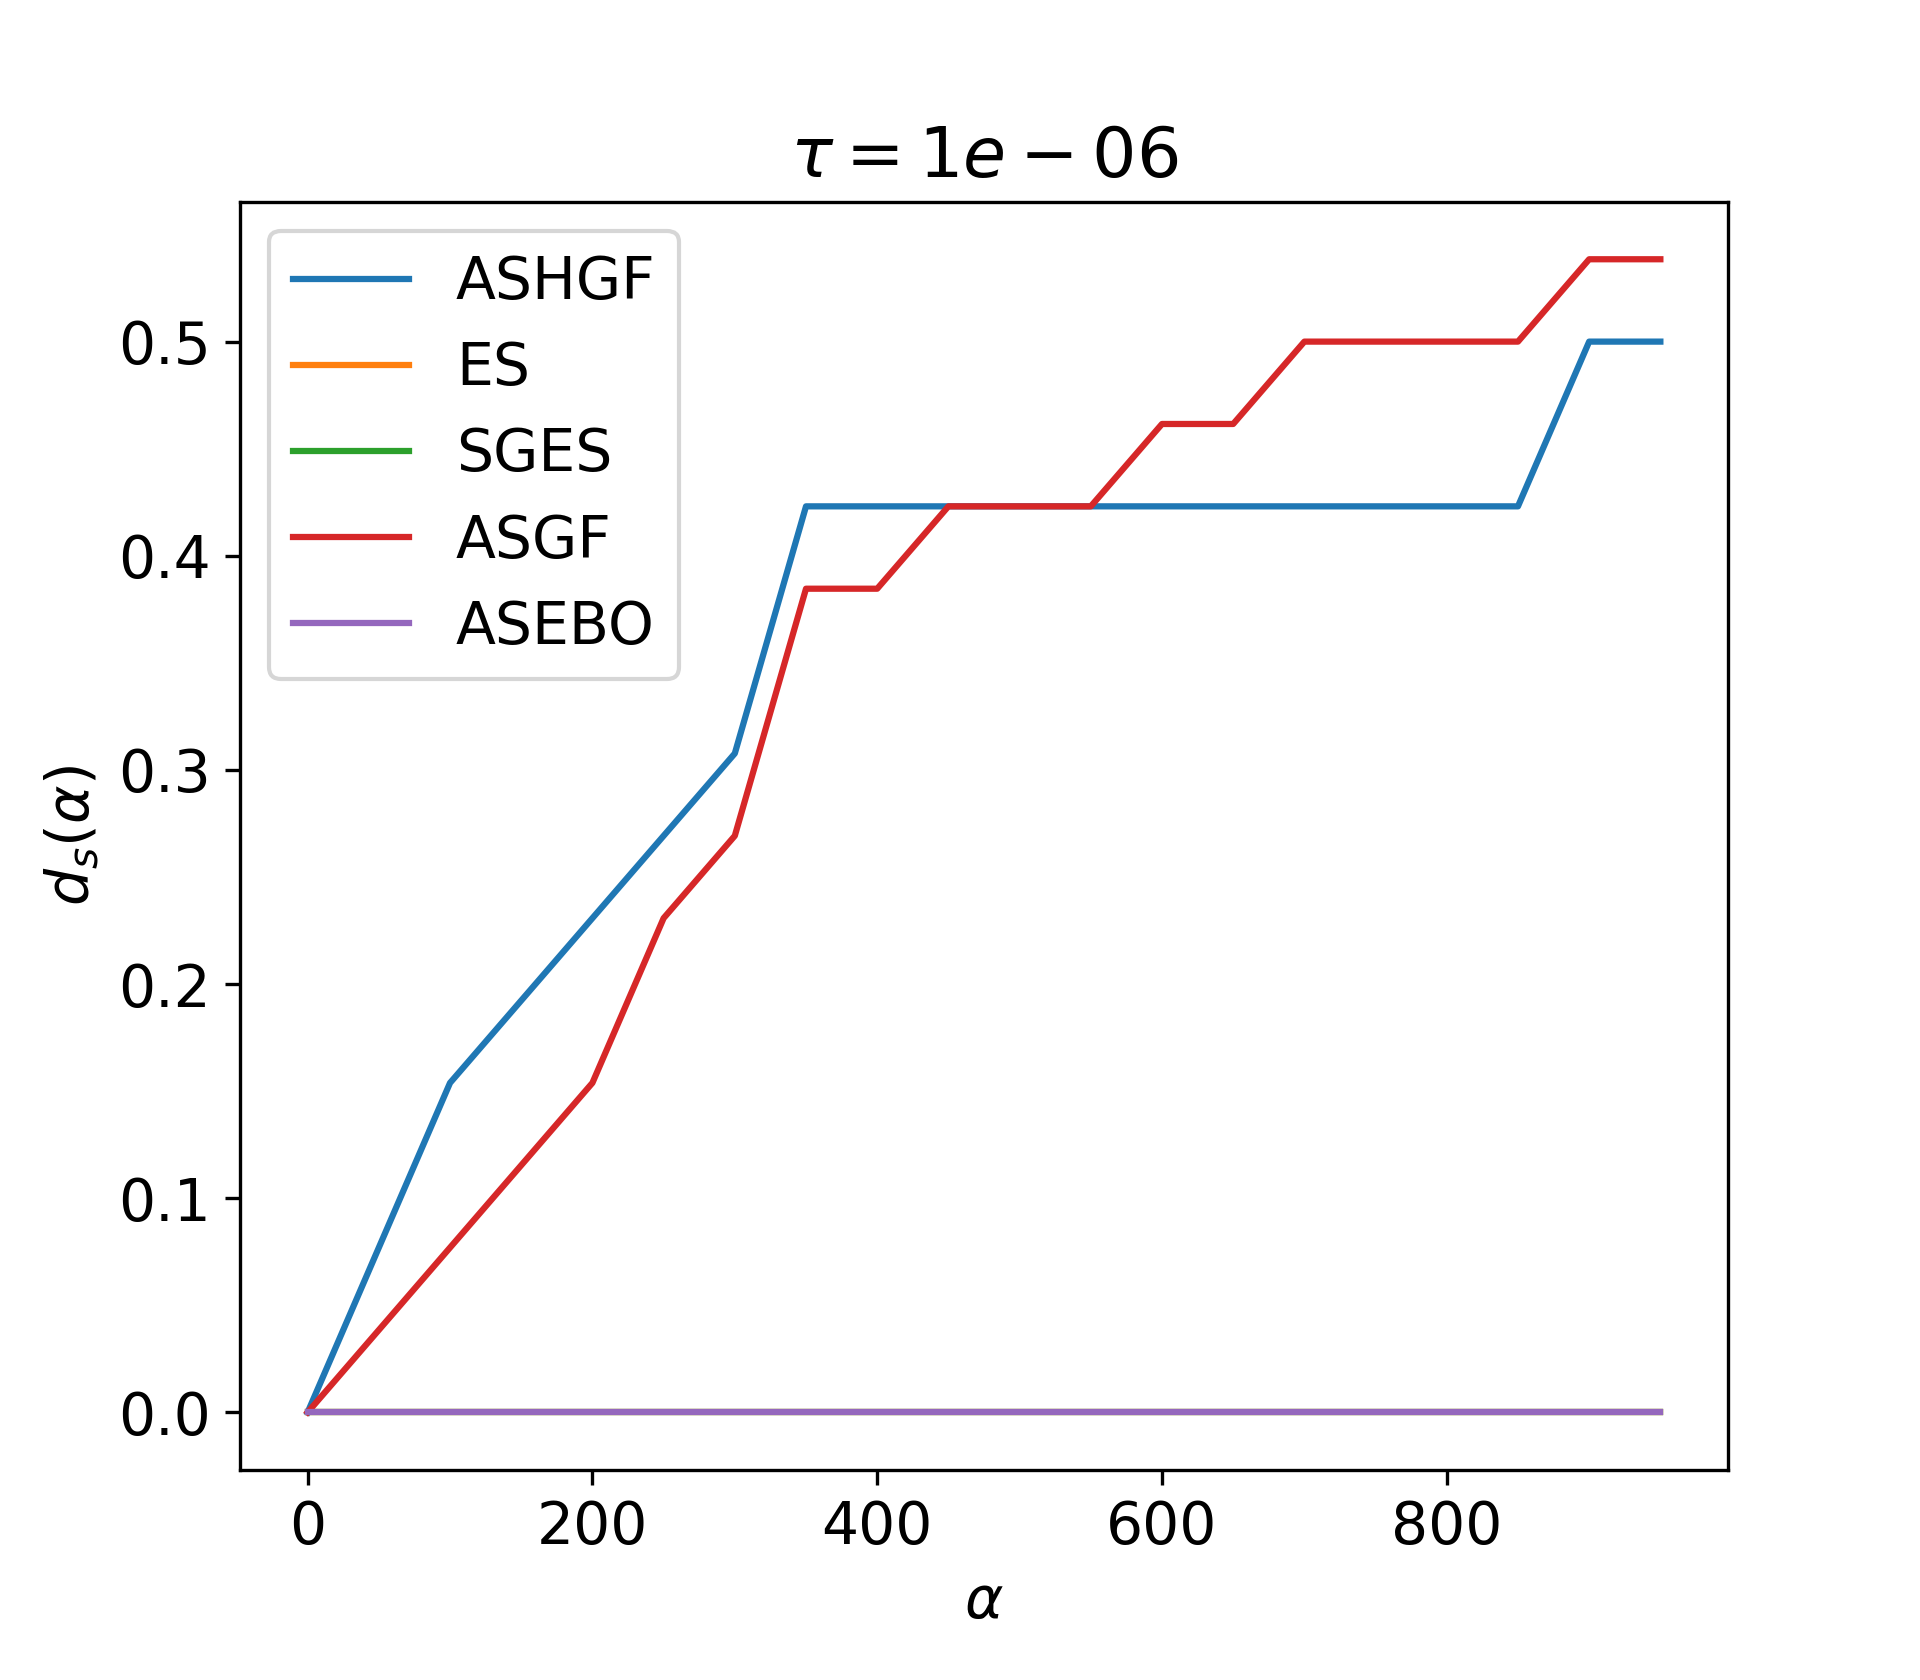
\includegraphics[width=1\textwidth]{figures/data_profiles/10/data_profile_10_100000000_1e-06.png}
	\end{subfigure}
	\centering
	\begin{subfigure}{0.3\textwidth}
		\centering 
		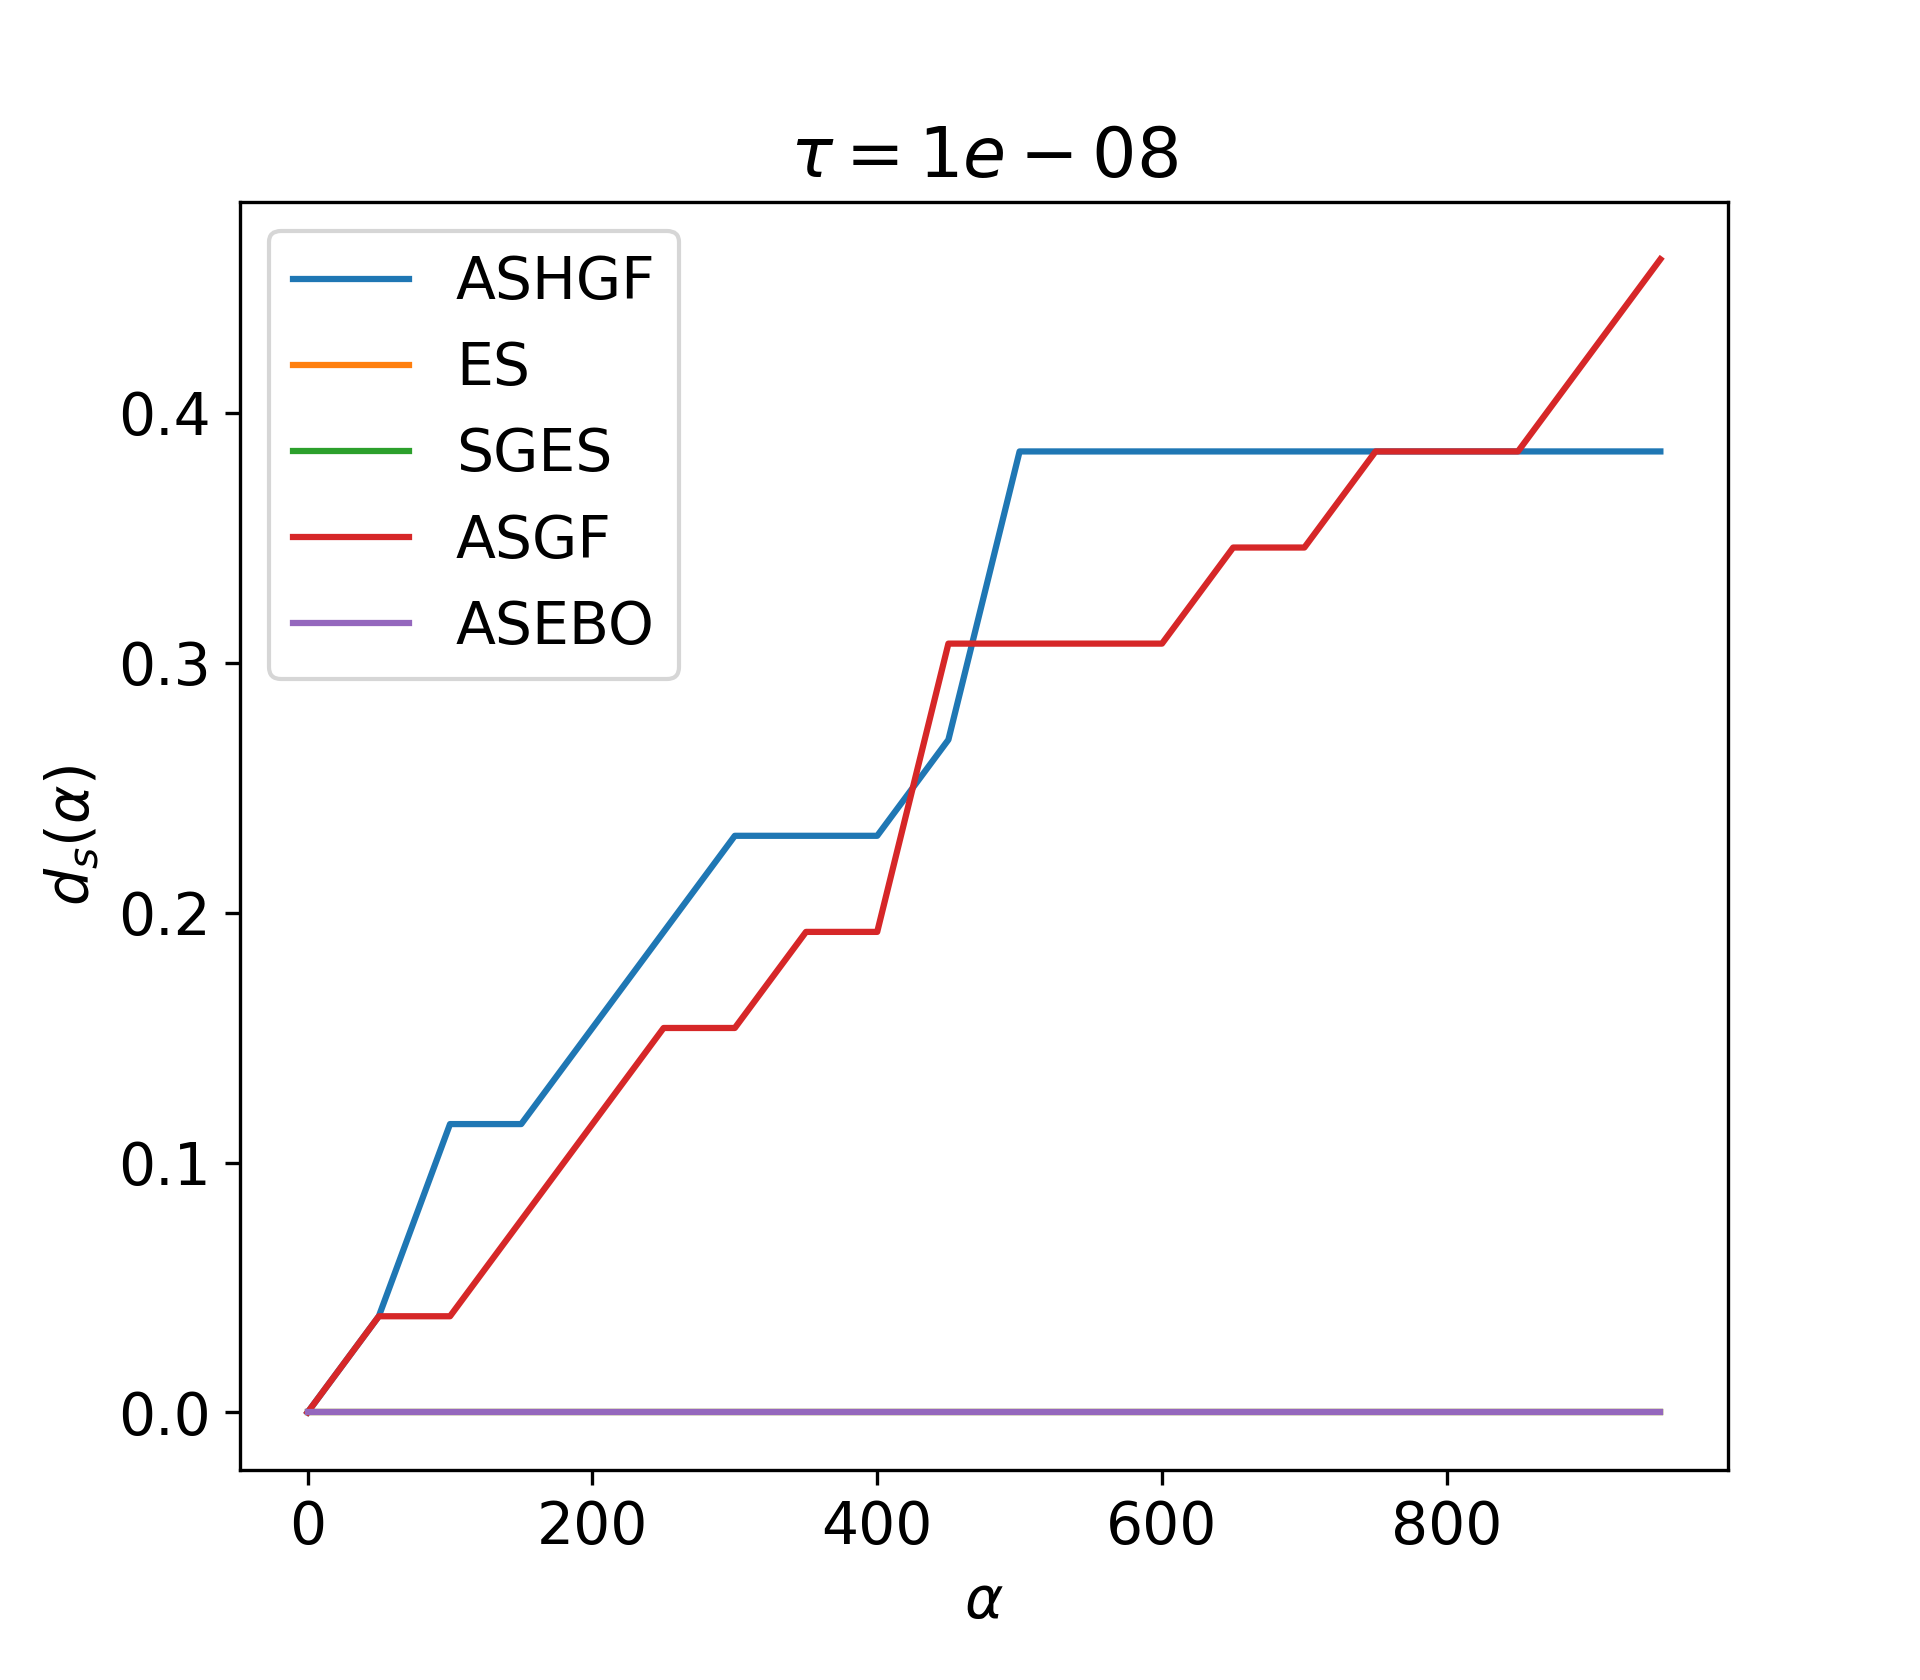
\includegraphics[width=1\textwidth]{figures/data_profiles/10/data_profile_10_100000000_1e-08.png}
	\end{subfigure}%
	\begin{subfigure}{0.3\textwidth}
		\centering 
		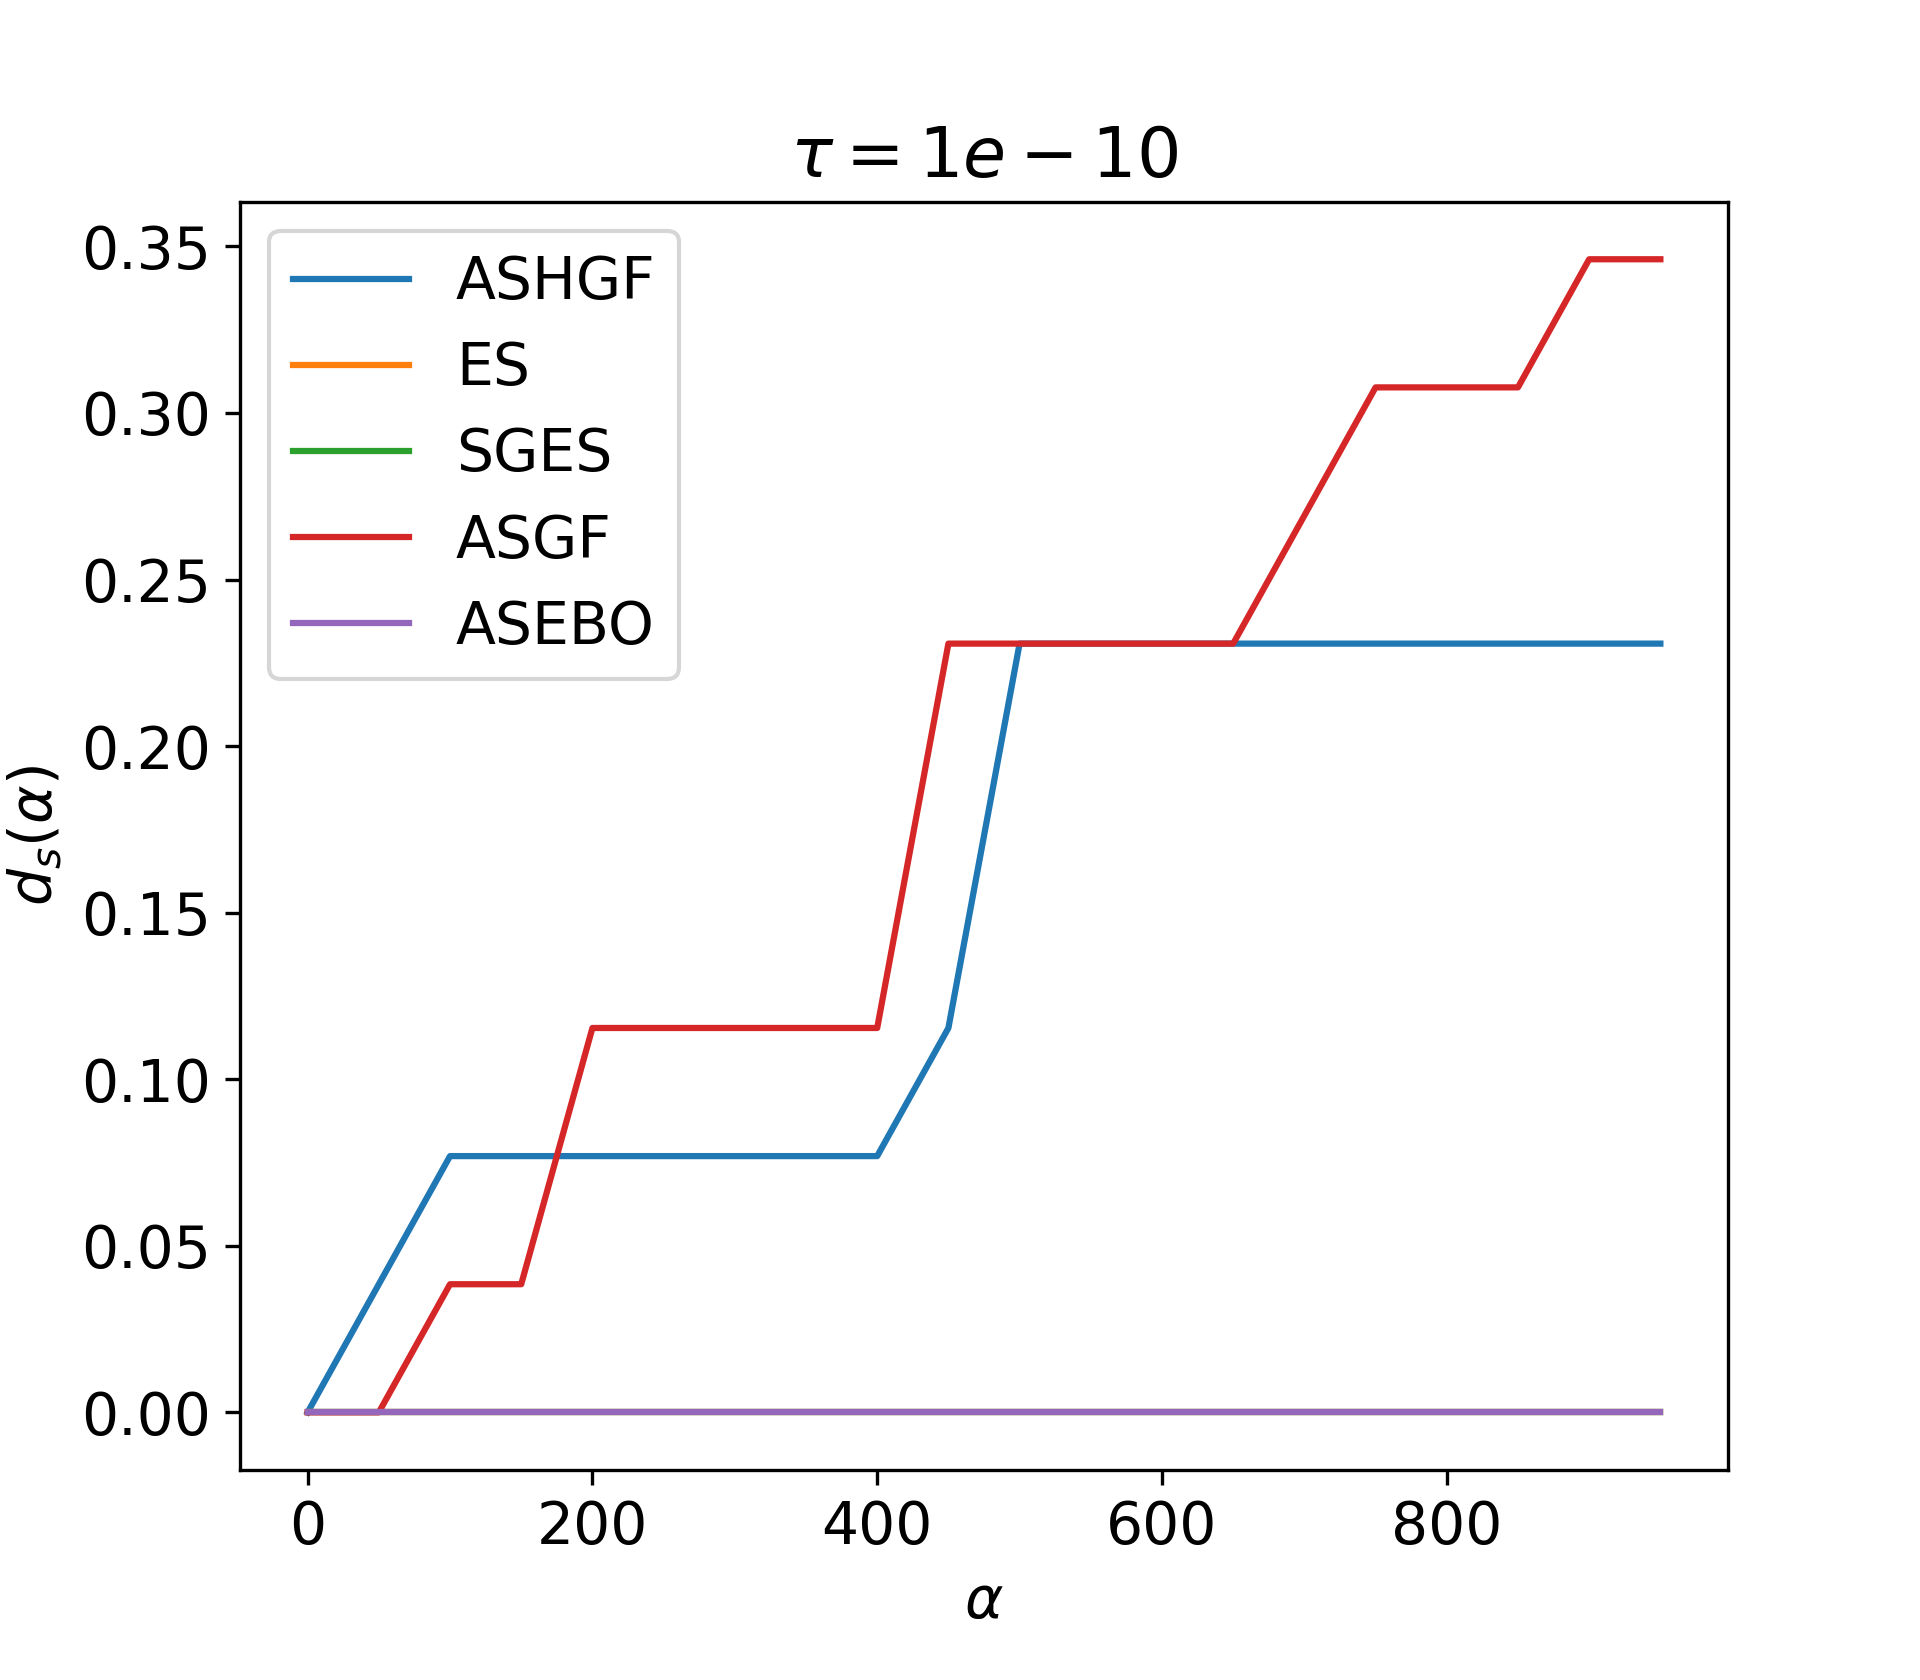
\includegraphics[width=1\textwidth]{figures/data_profiles/10/data_profile_10_100000000_1e-10.png}
	\end{subfigure}
	\caption{Data profiles with $\mu_L = 10^{8}$}
	\label{DataProfiles10Mu100000000}
\end{figure}

\subsubsection{Dimension 100}

\begin{figure}[H]
\centering
\begin{subfigure}{0.3\textwidth}
  \centering 
  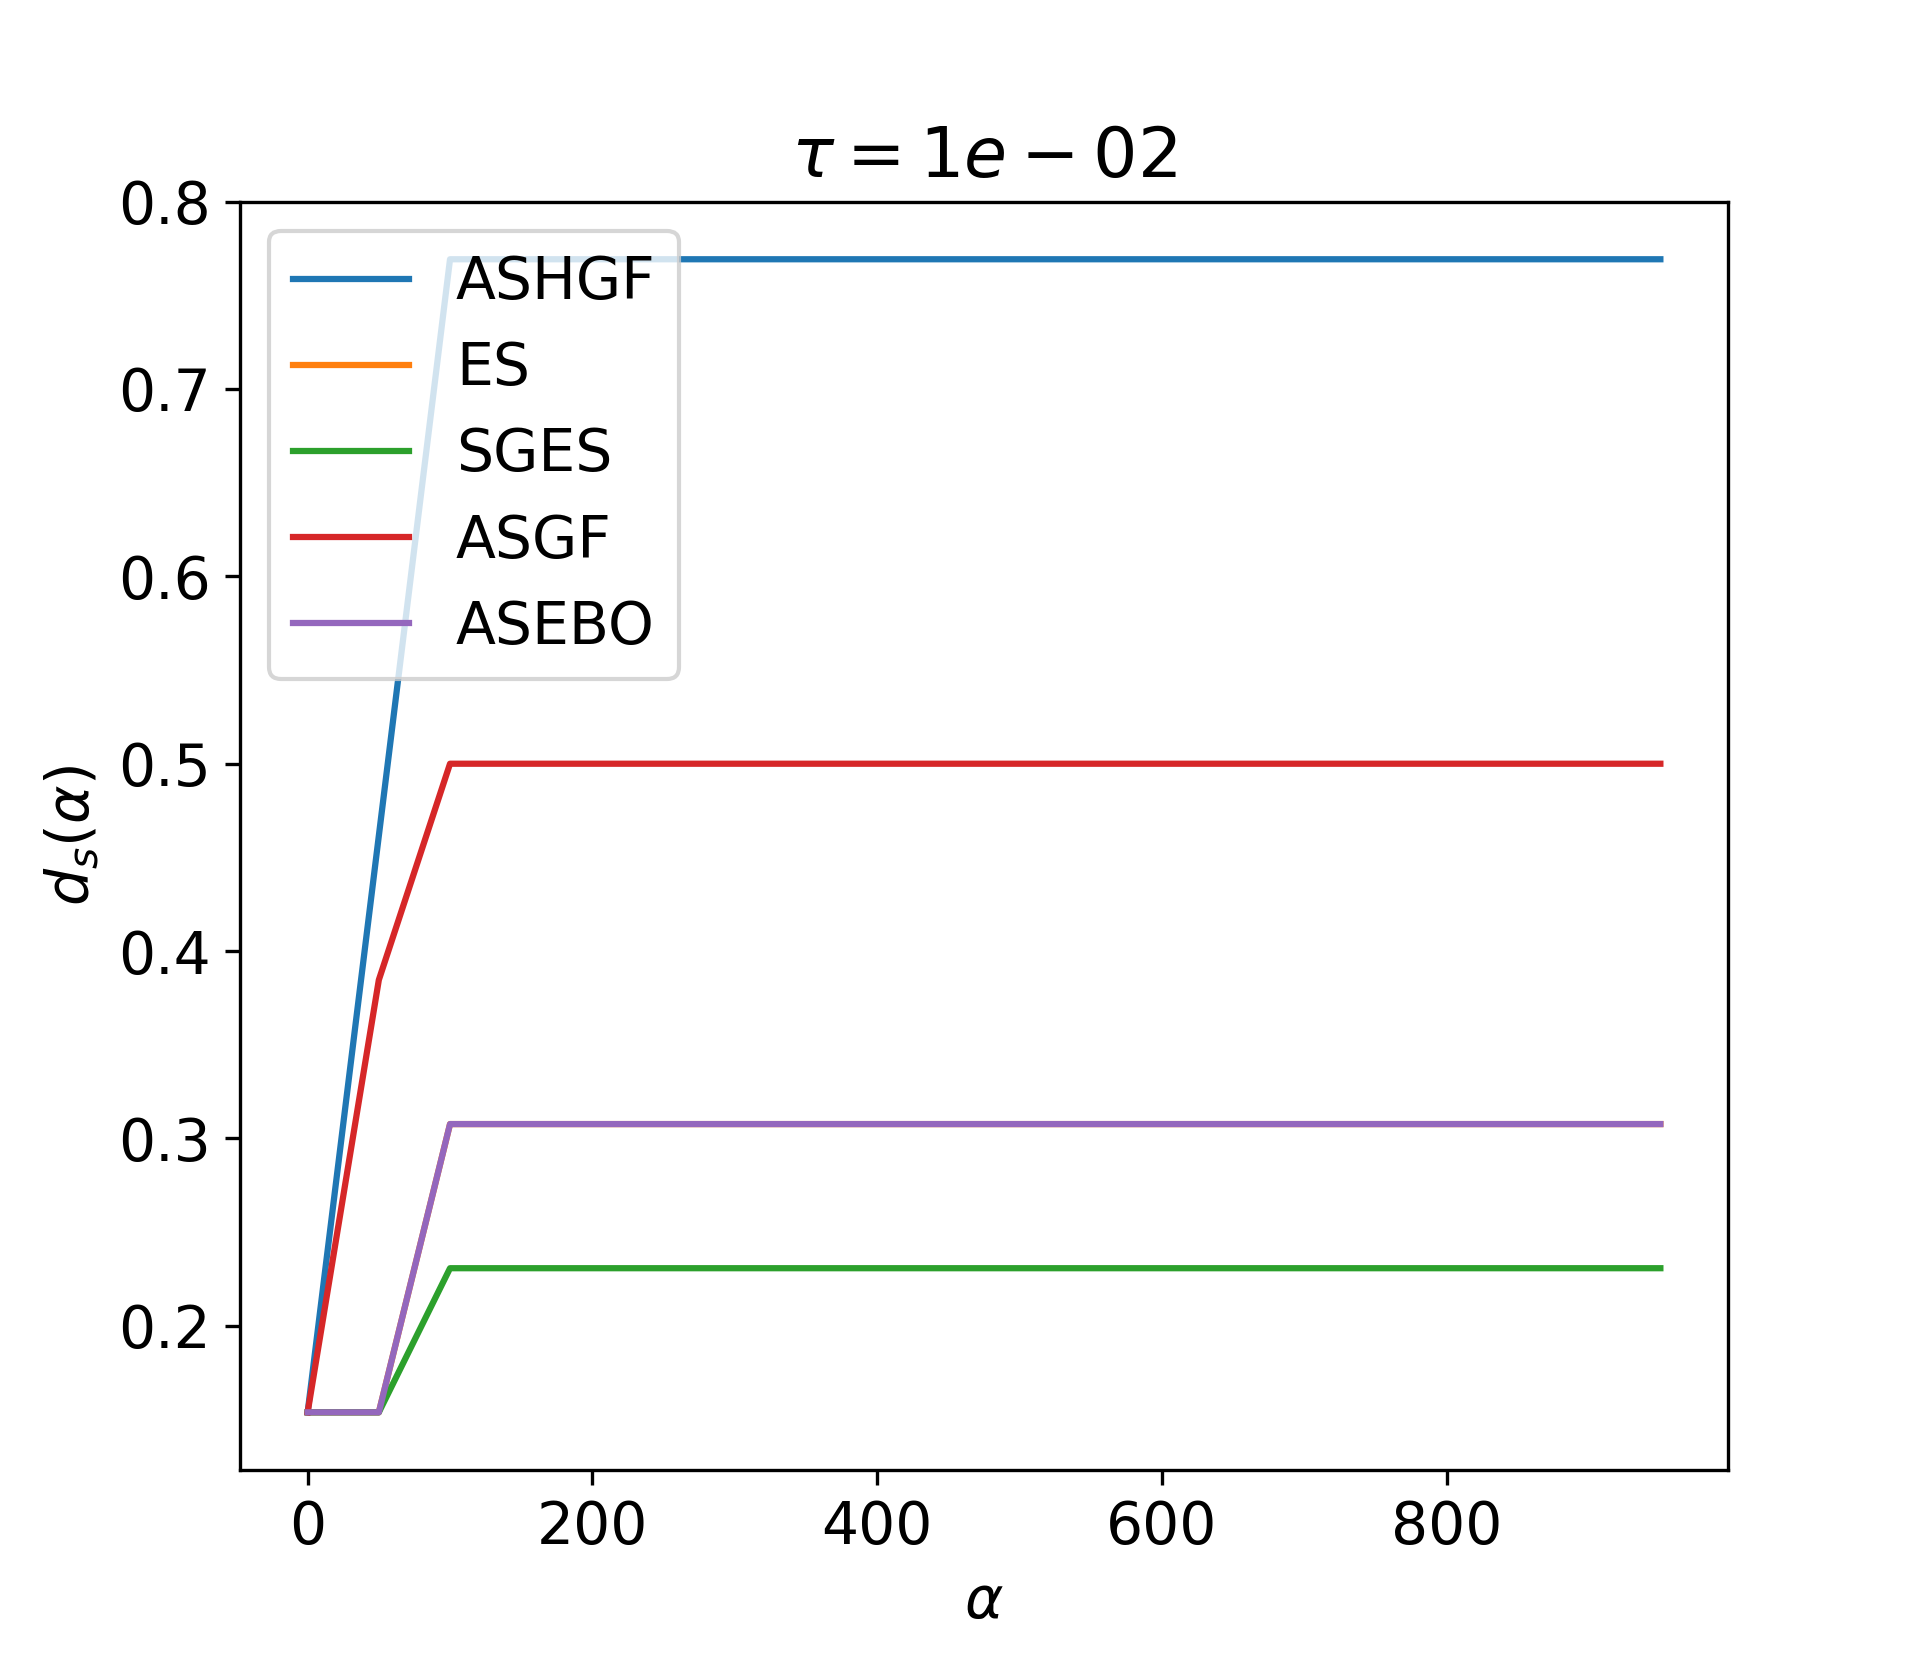
\includegraphics[width=1\textwidth]{figures/data_profiles/100/data_profile_100_10000_1e-02.png}
\end{subfigure}%
\begin{subfigure}{0.3\textwidth}
  \centering 
  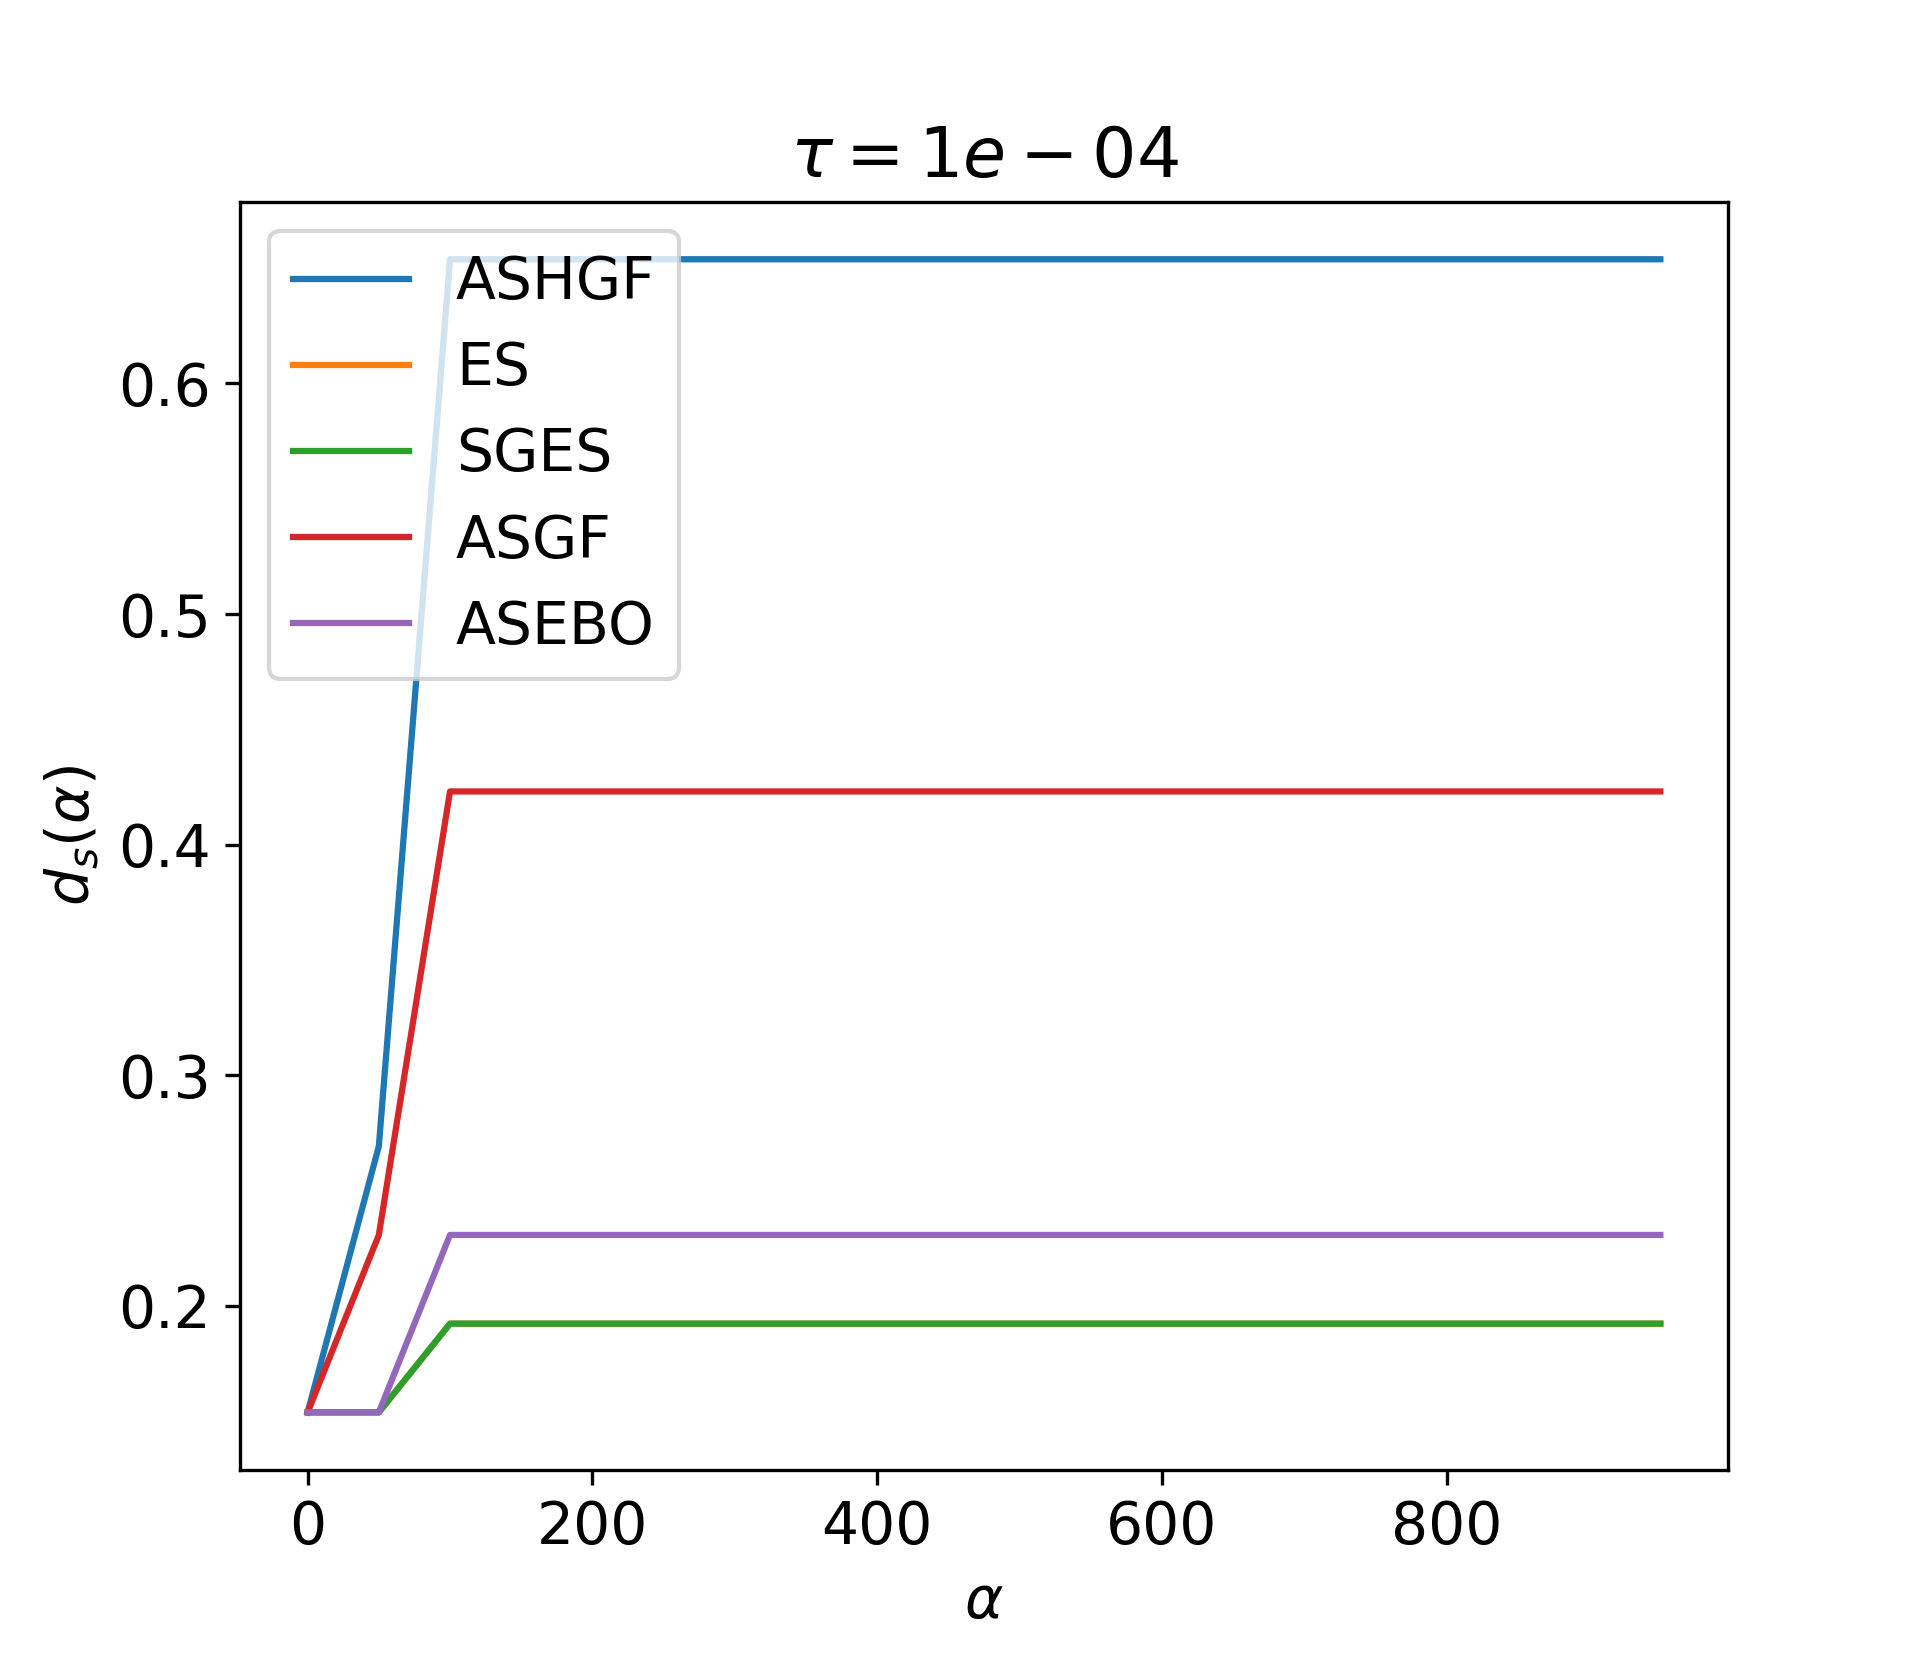
\includegraphics[width=1\textwidth]{figures/data_profiles/100/data_profile_100_10000_1e-04.png}
\end{subfigure}
\begin{subfigure}{0.3\textwidth}
  \centering 
  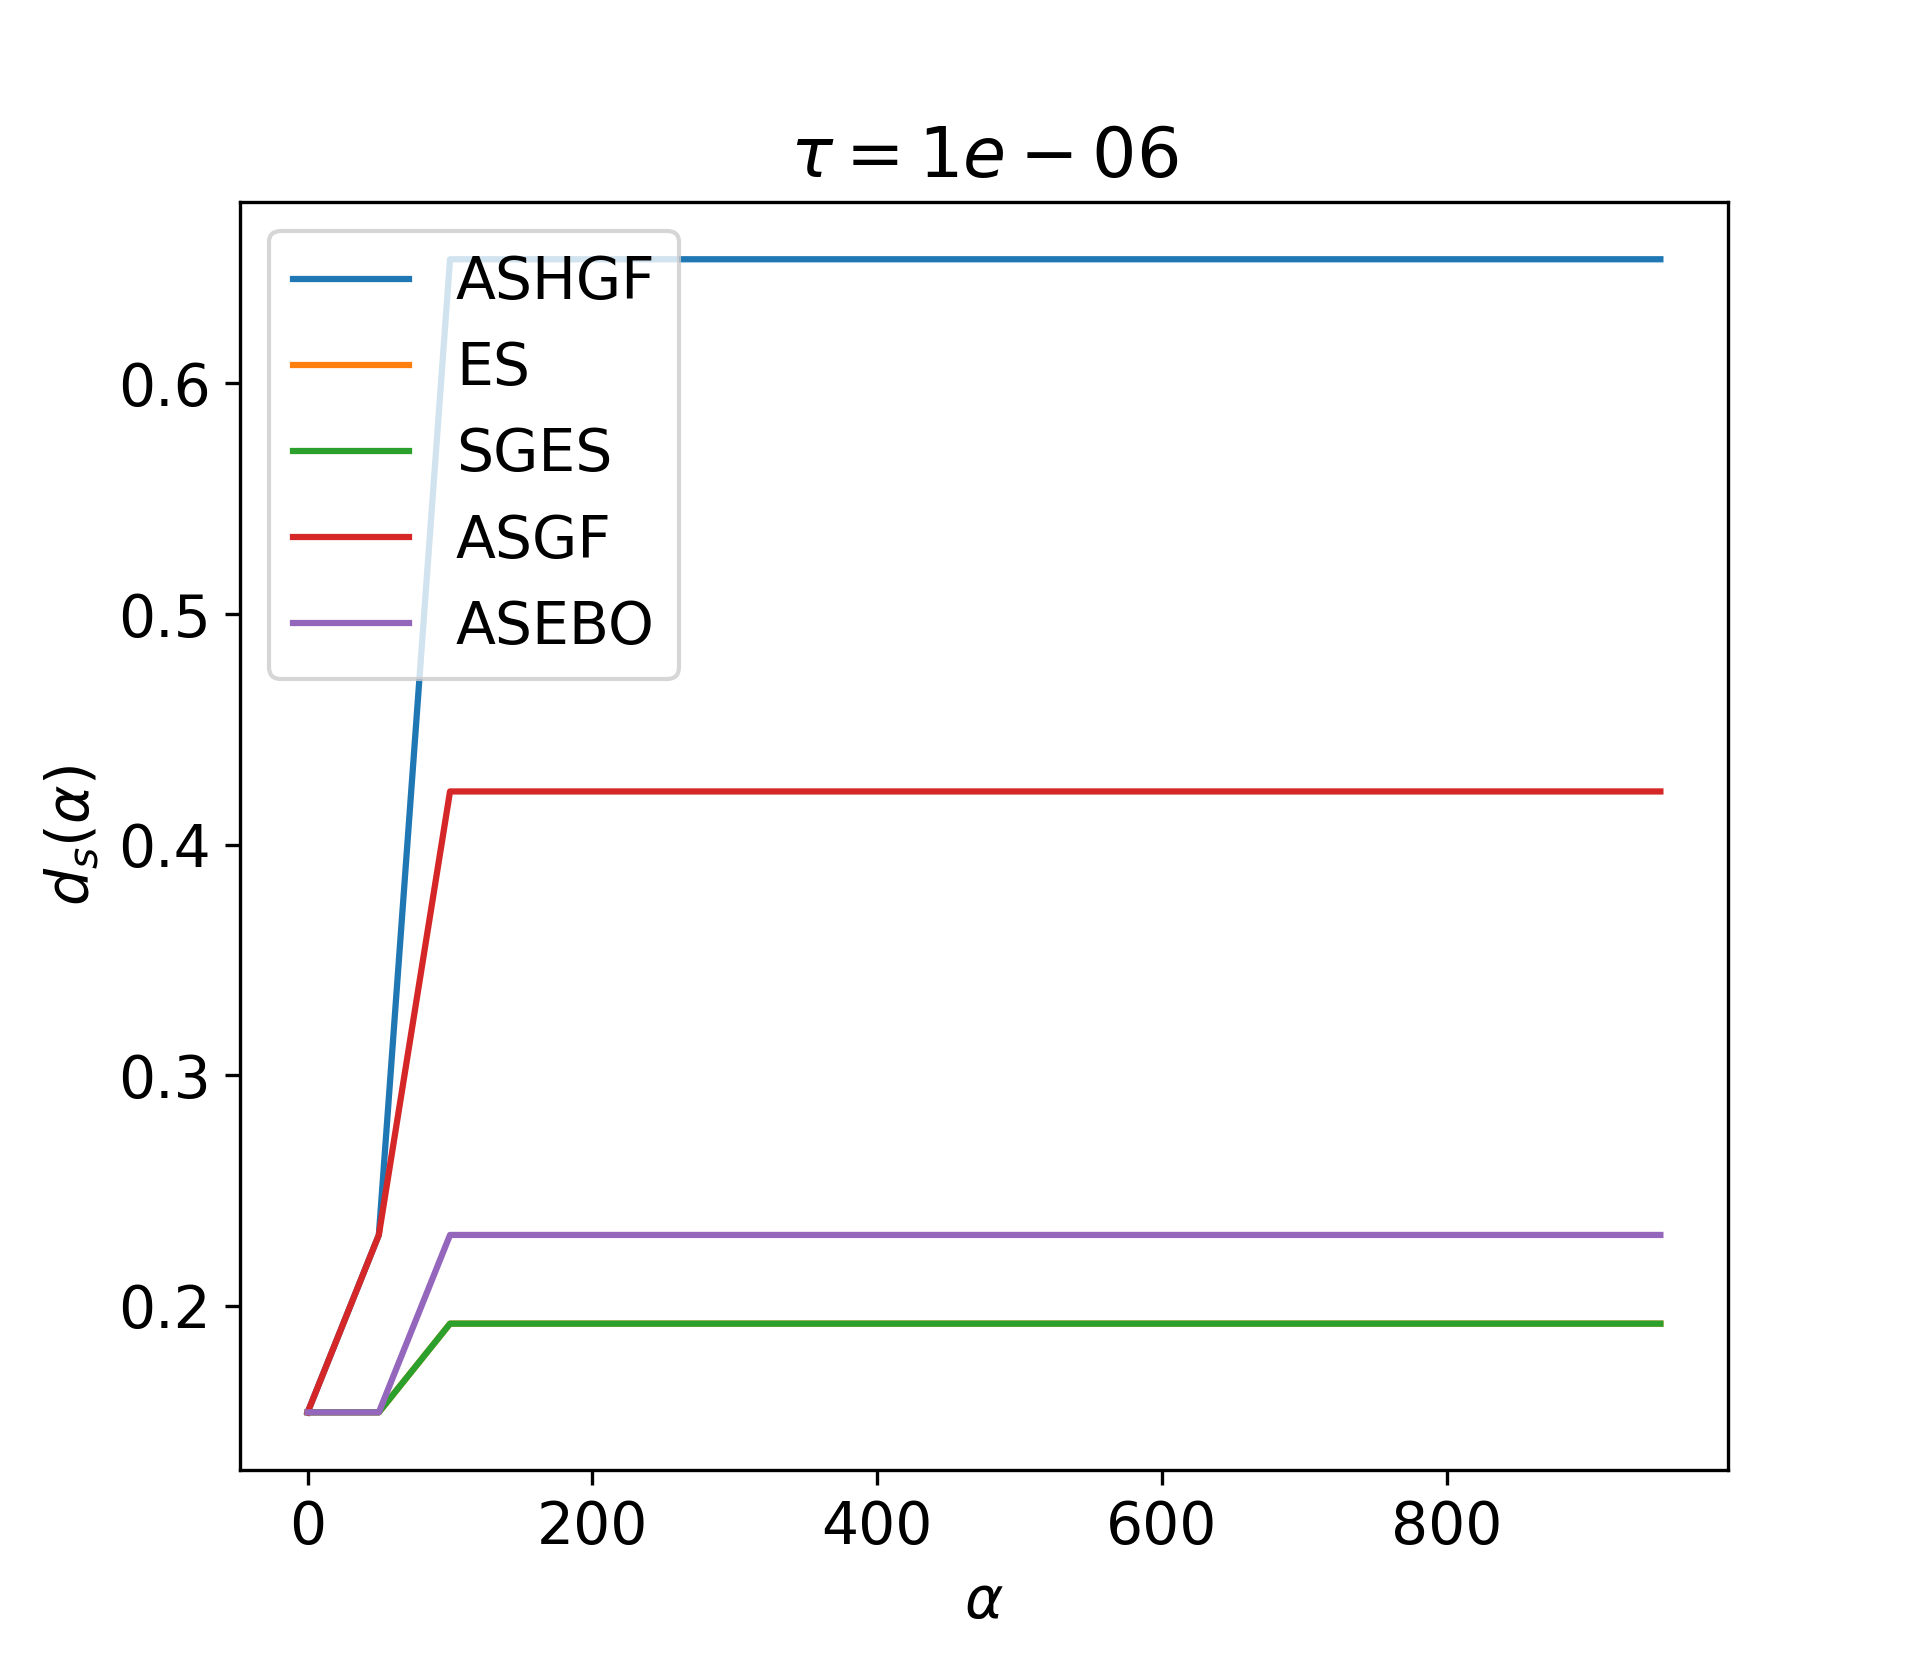
\includegraphics[width=1\textwidth]{figures/data_profiles/100/data_profile_100_10000_1e-06.png}
\end{subfigure}
\centering
\begin{subfigure}{0.3\textwidth}
  \centering 
  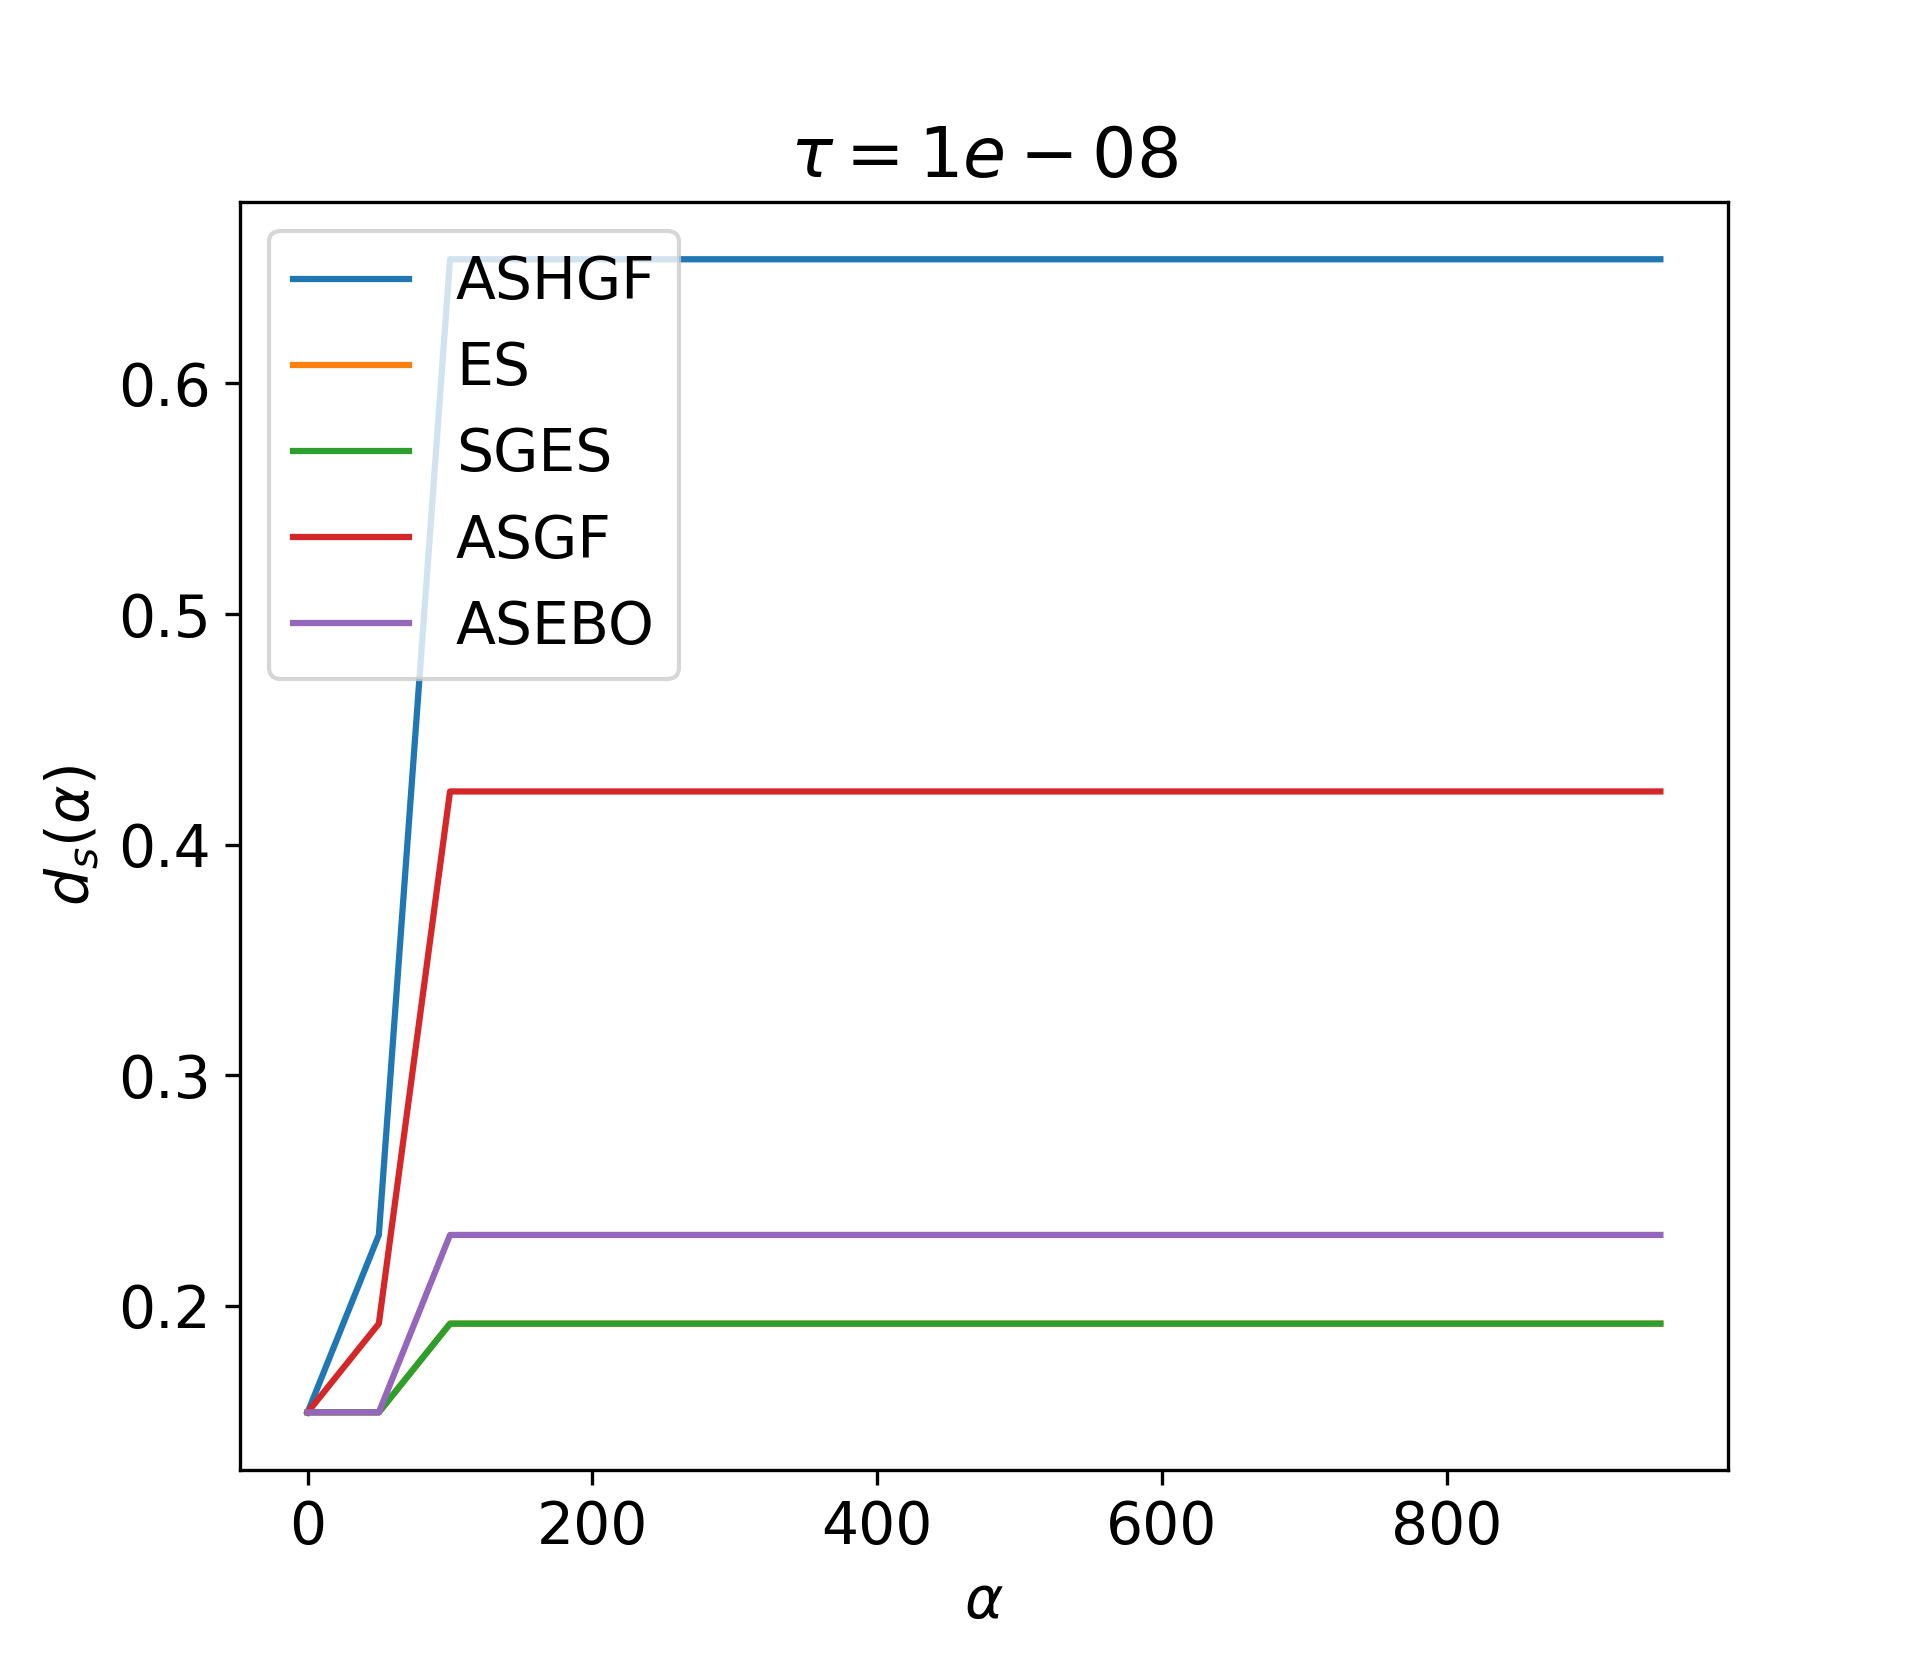
\includegraphics[width=1\textwidth]{figures/data_profiles/100/data_profile_100_10000_1e-08.png}
\end{subfigure}%
\begin{subfigure}{0.3\textwidth}
  \centering 
  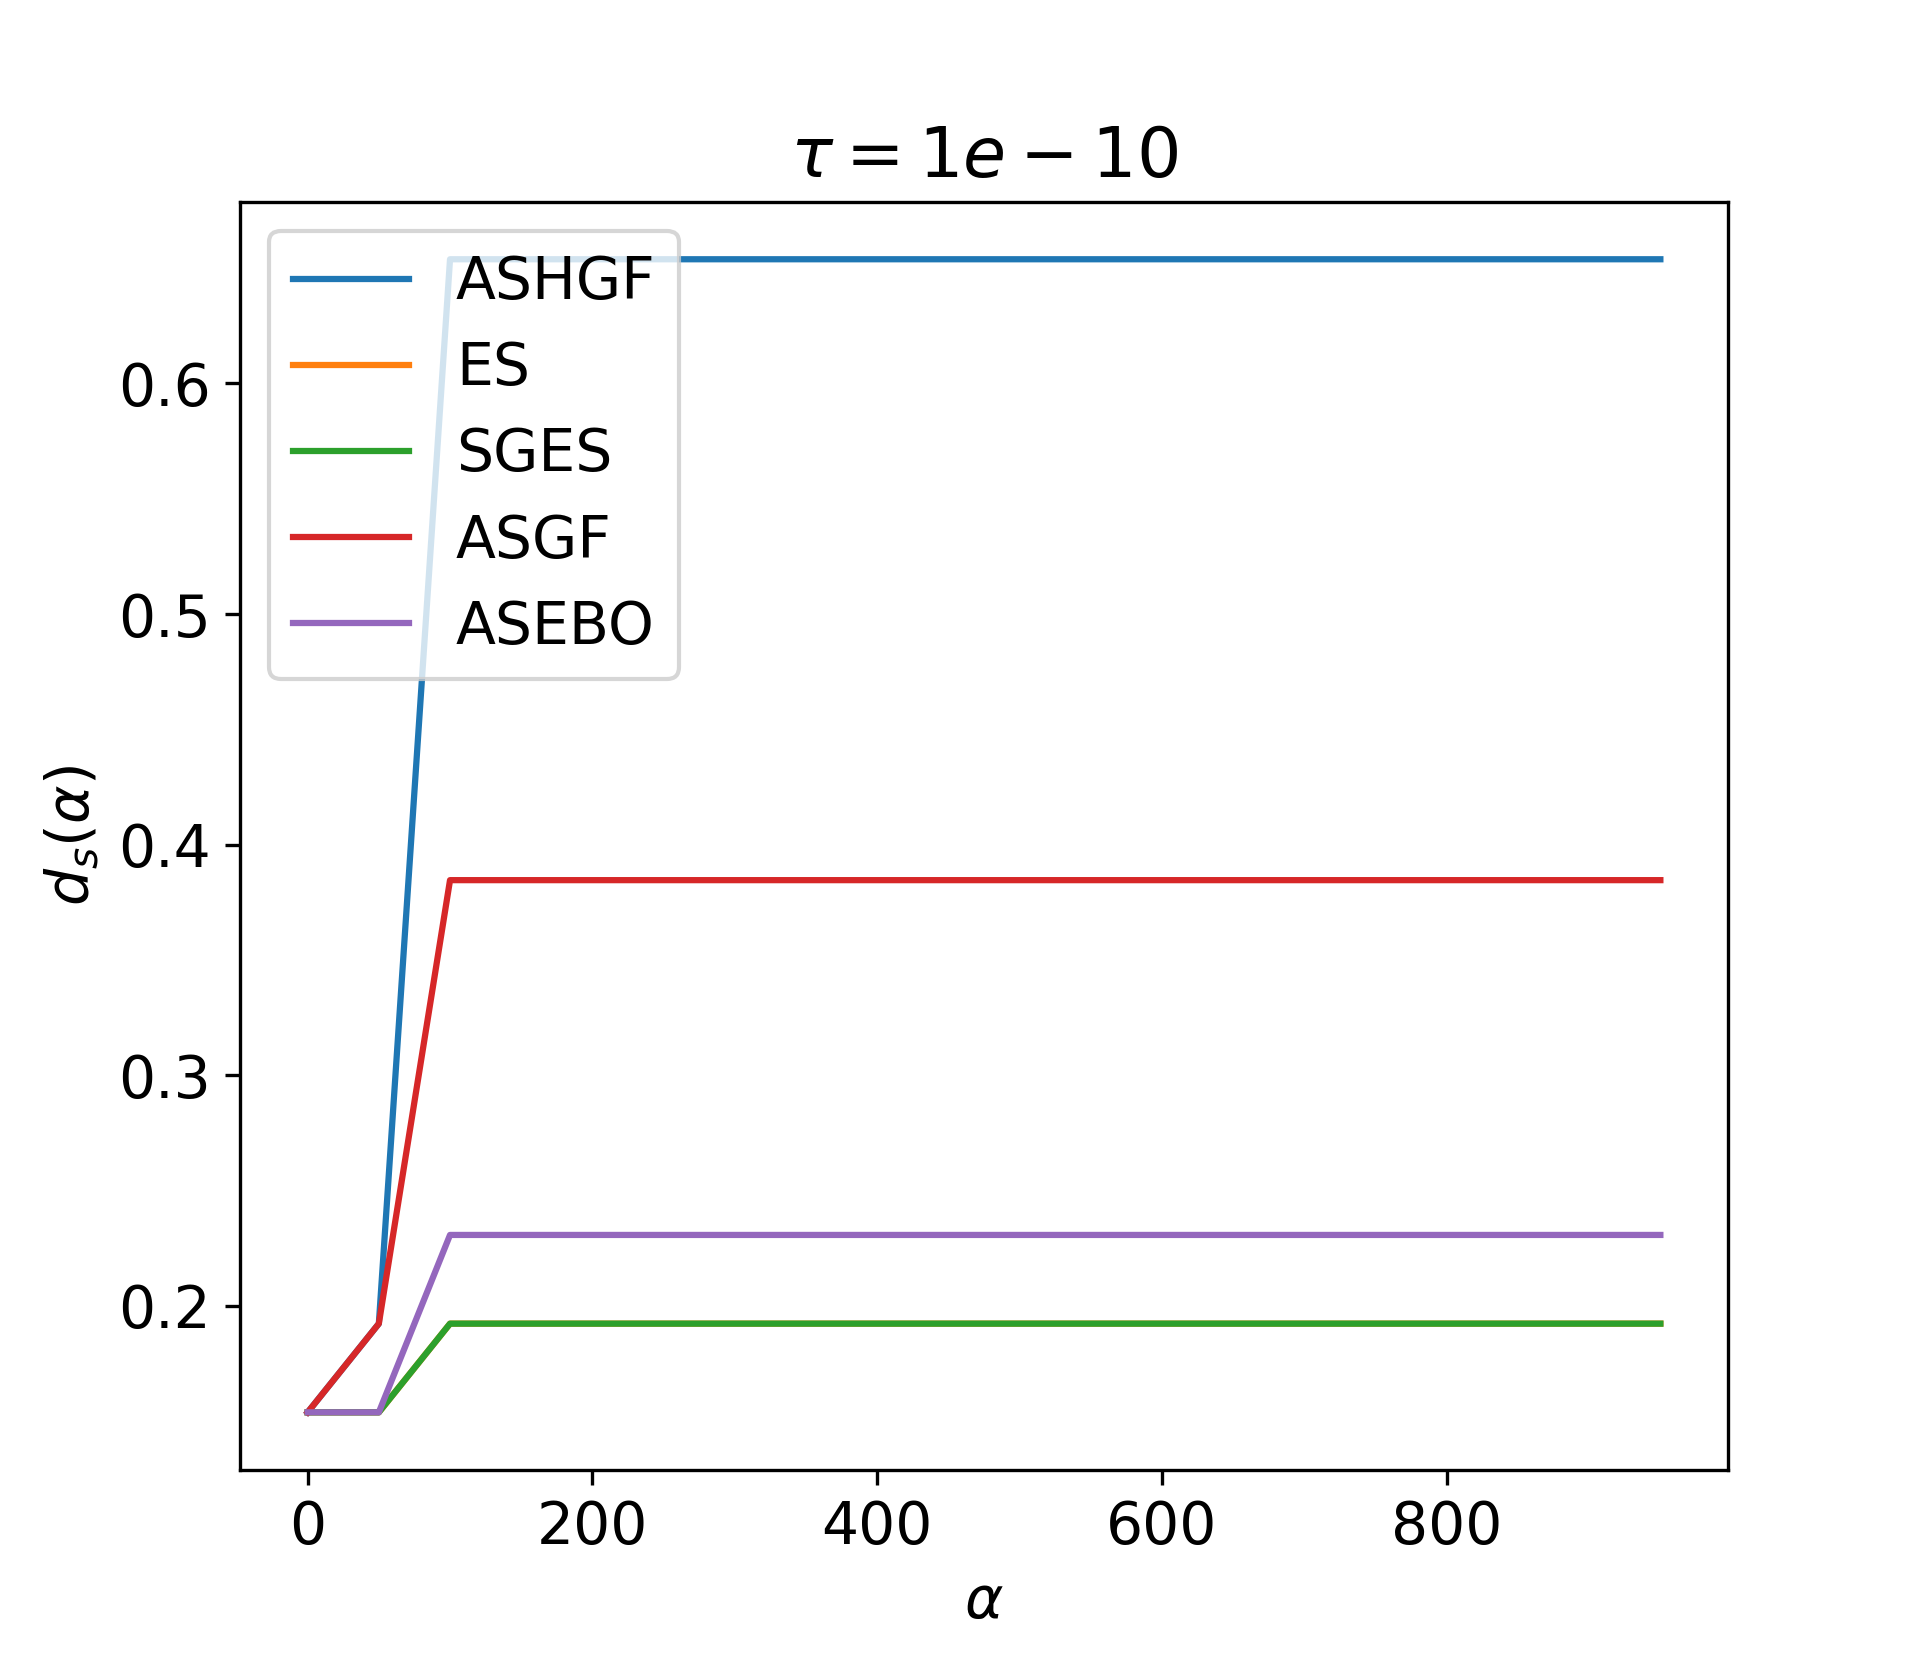
\includegraphics[width=1\textwidth]{figures/data_profiles/100/data_profile_100_10000_1e-10.png}
\end{subfigure}
\caption{Data profiles with $\mu_L = 10^{4}$}
\label{DataProfiles100Mu10000}
\end{figure}

\begin{figure}[H]
\centering
\begin{subfigure}{0.3\textwidth}
  \centering 
  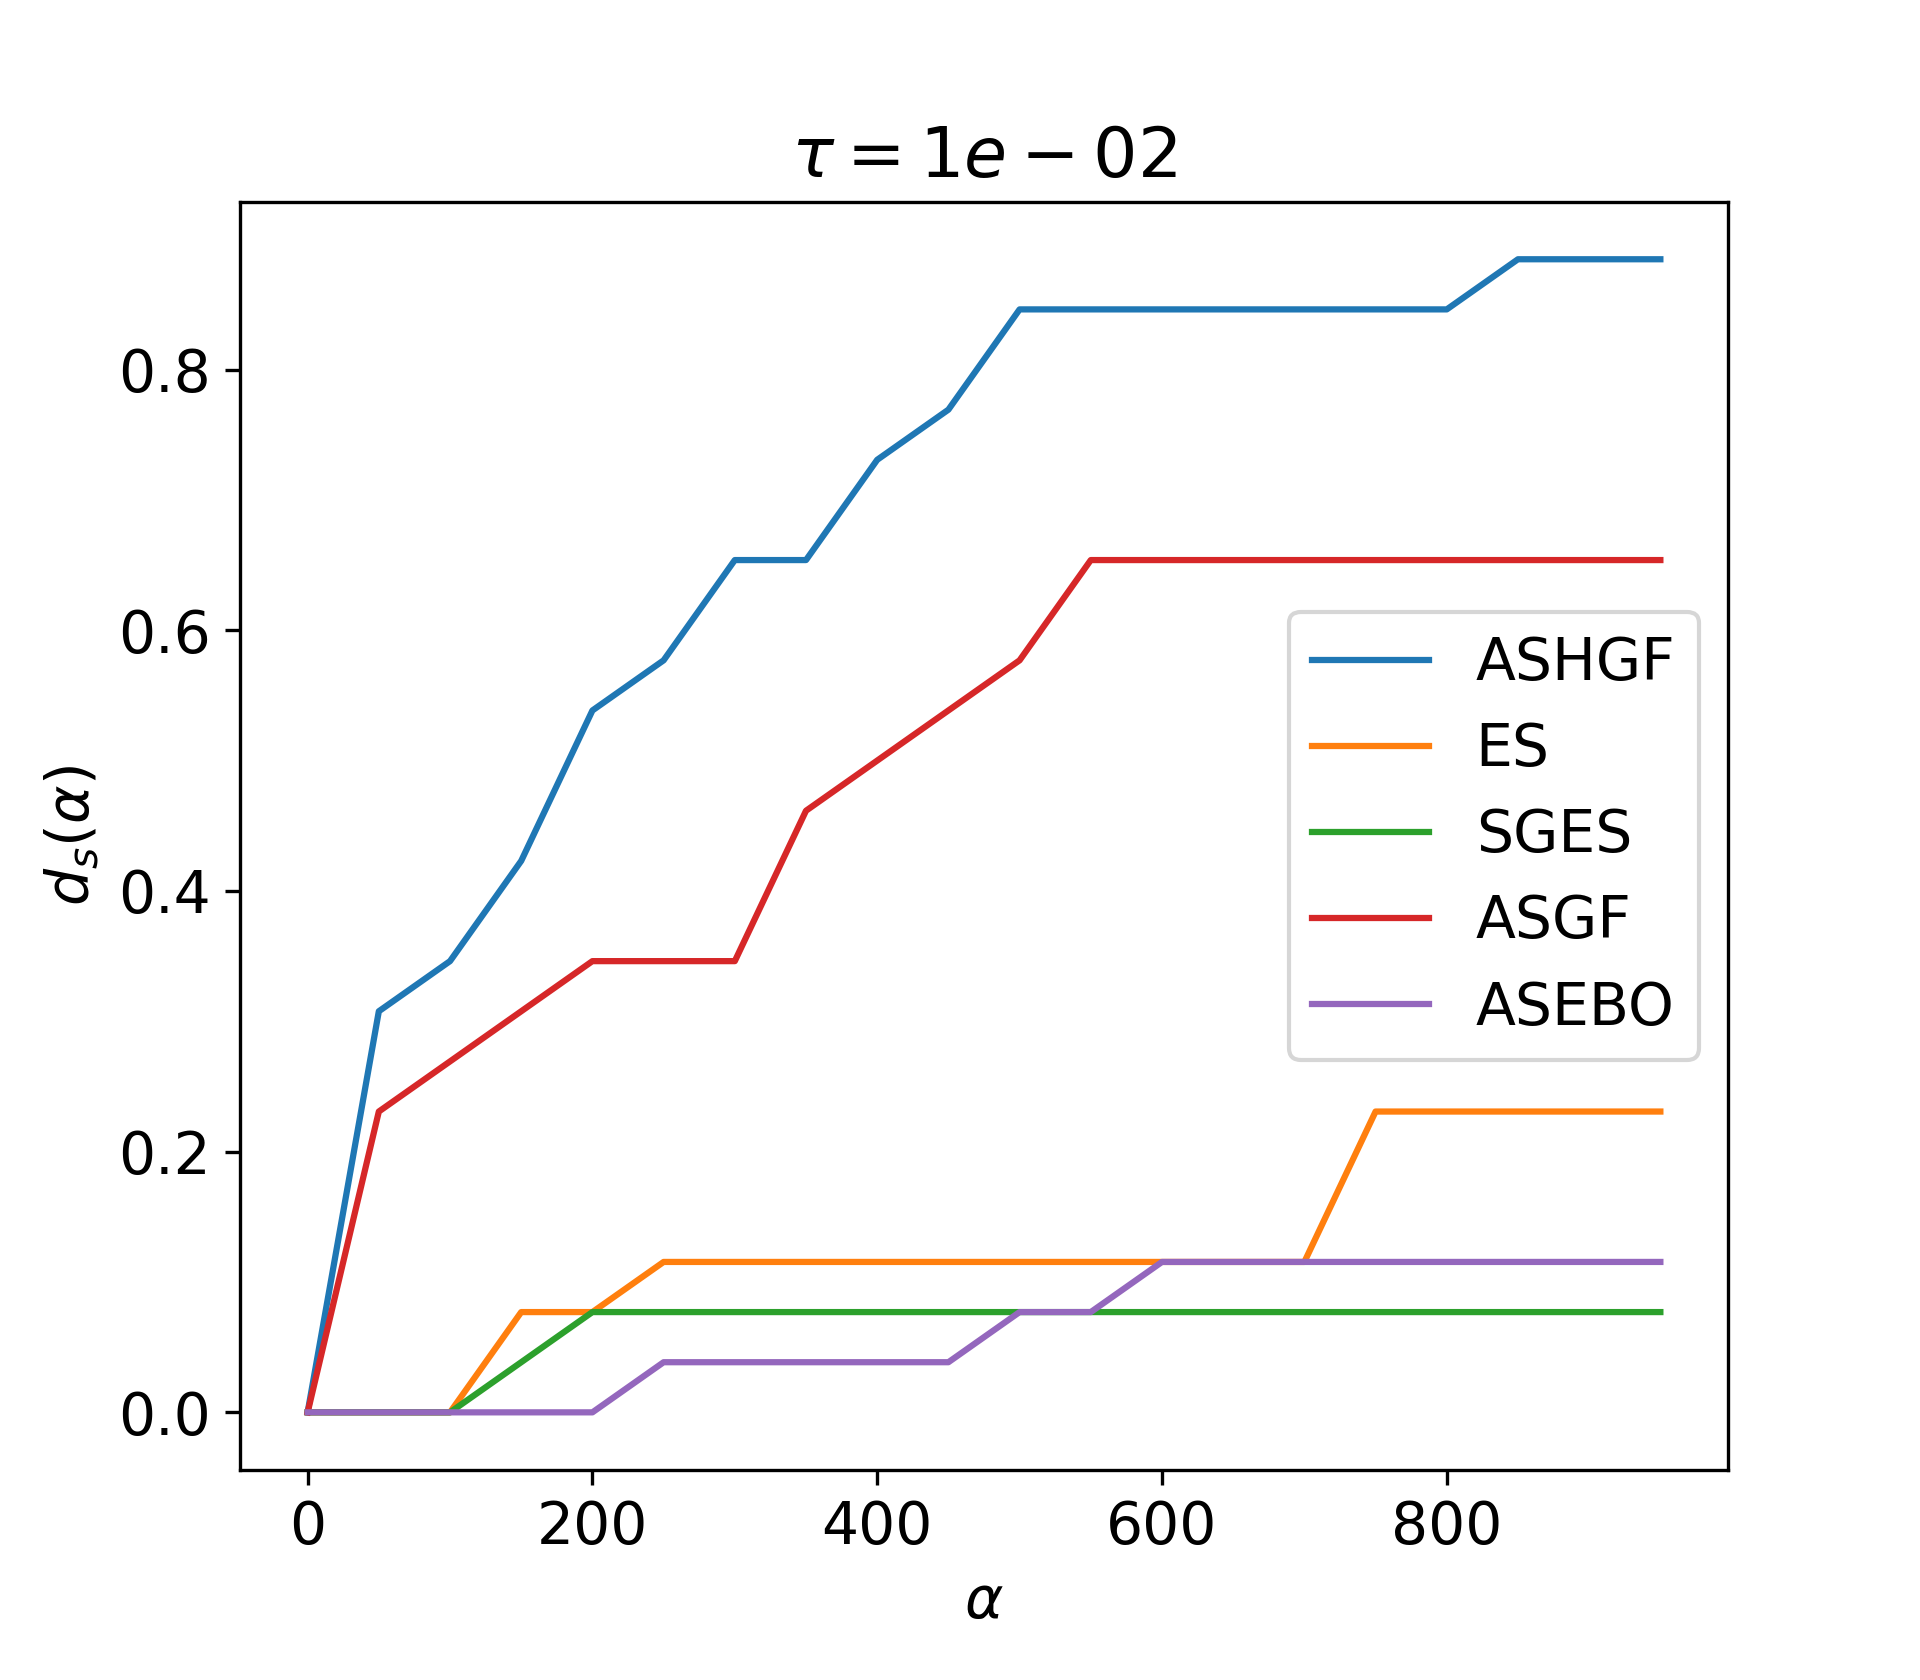
\includegraphics[width=1\textwidth]{figures/data_profiles/100/data_profile_100_100000_1e-02.png}
\end{subfigure}%
\begin{subfigure}{0.3\textwidth}
  \centering 
  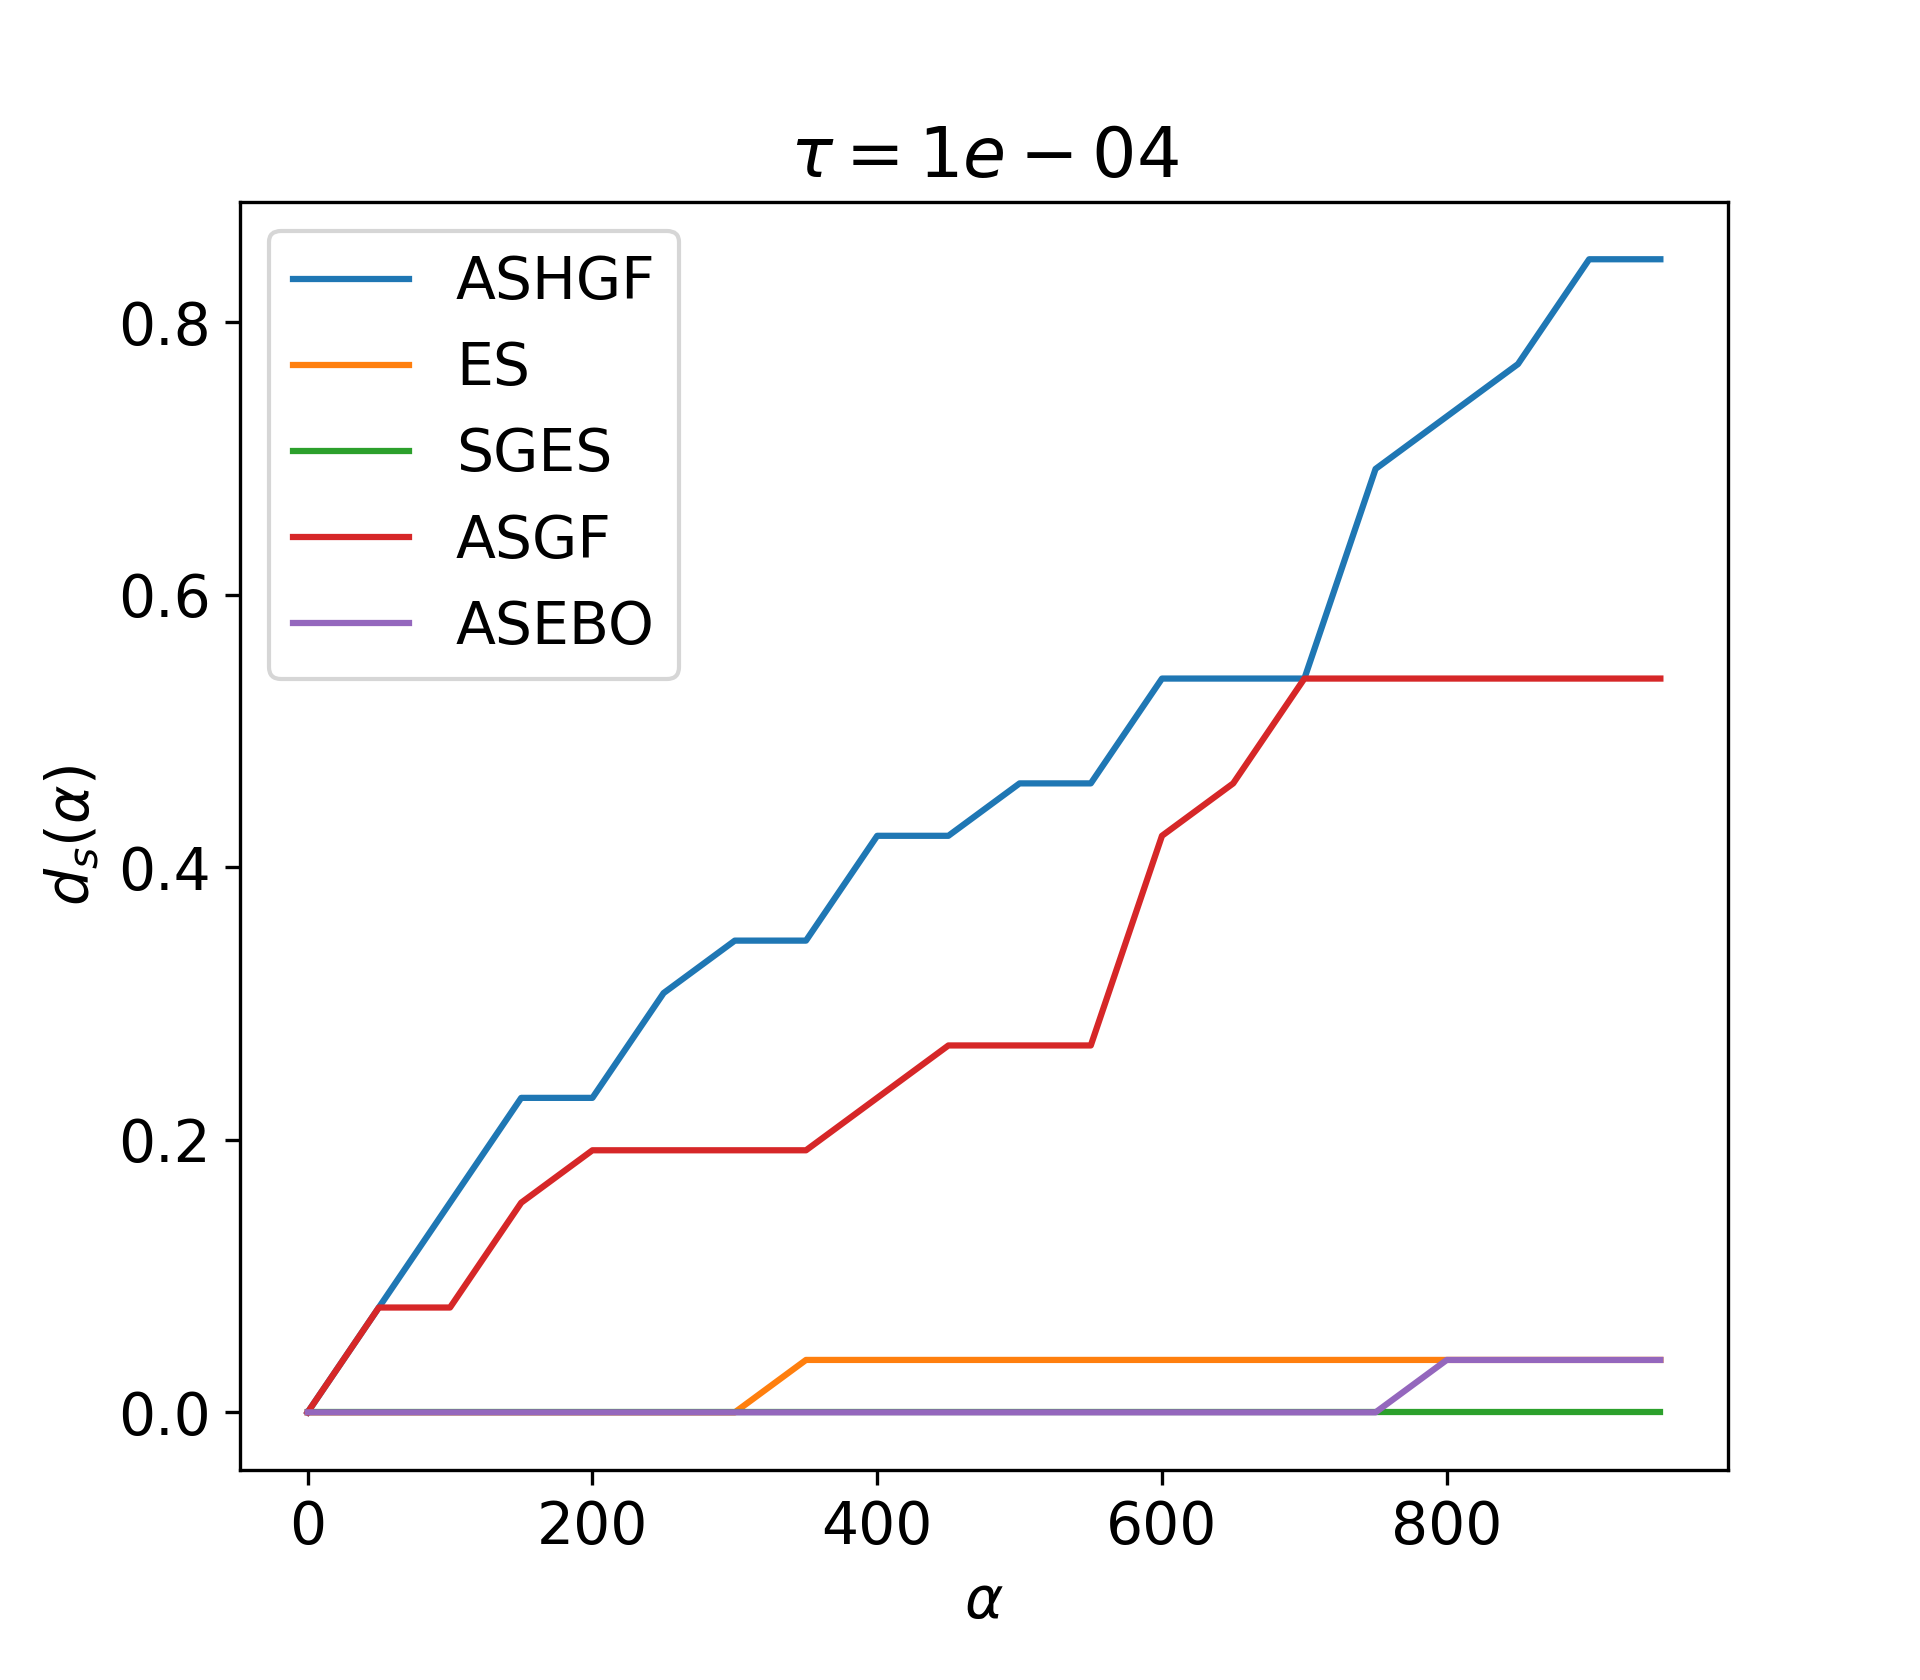
\includegraphics[width=1\textwidth]{figures/data_profiles/100/data_profile_100_100000_1e-04.png}
\end{subfigure}
\begin{subfigure}{0.3\textwidth}
  \centering 
  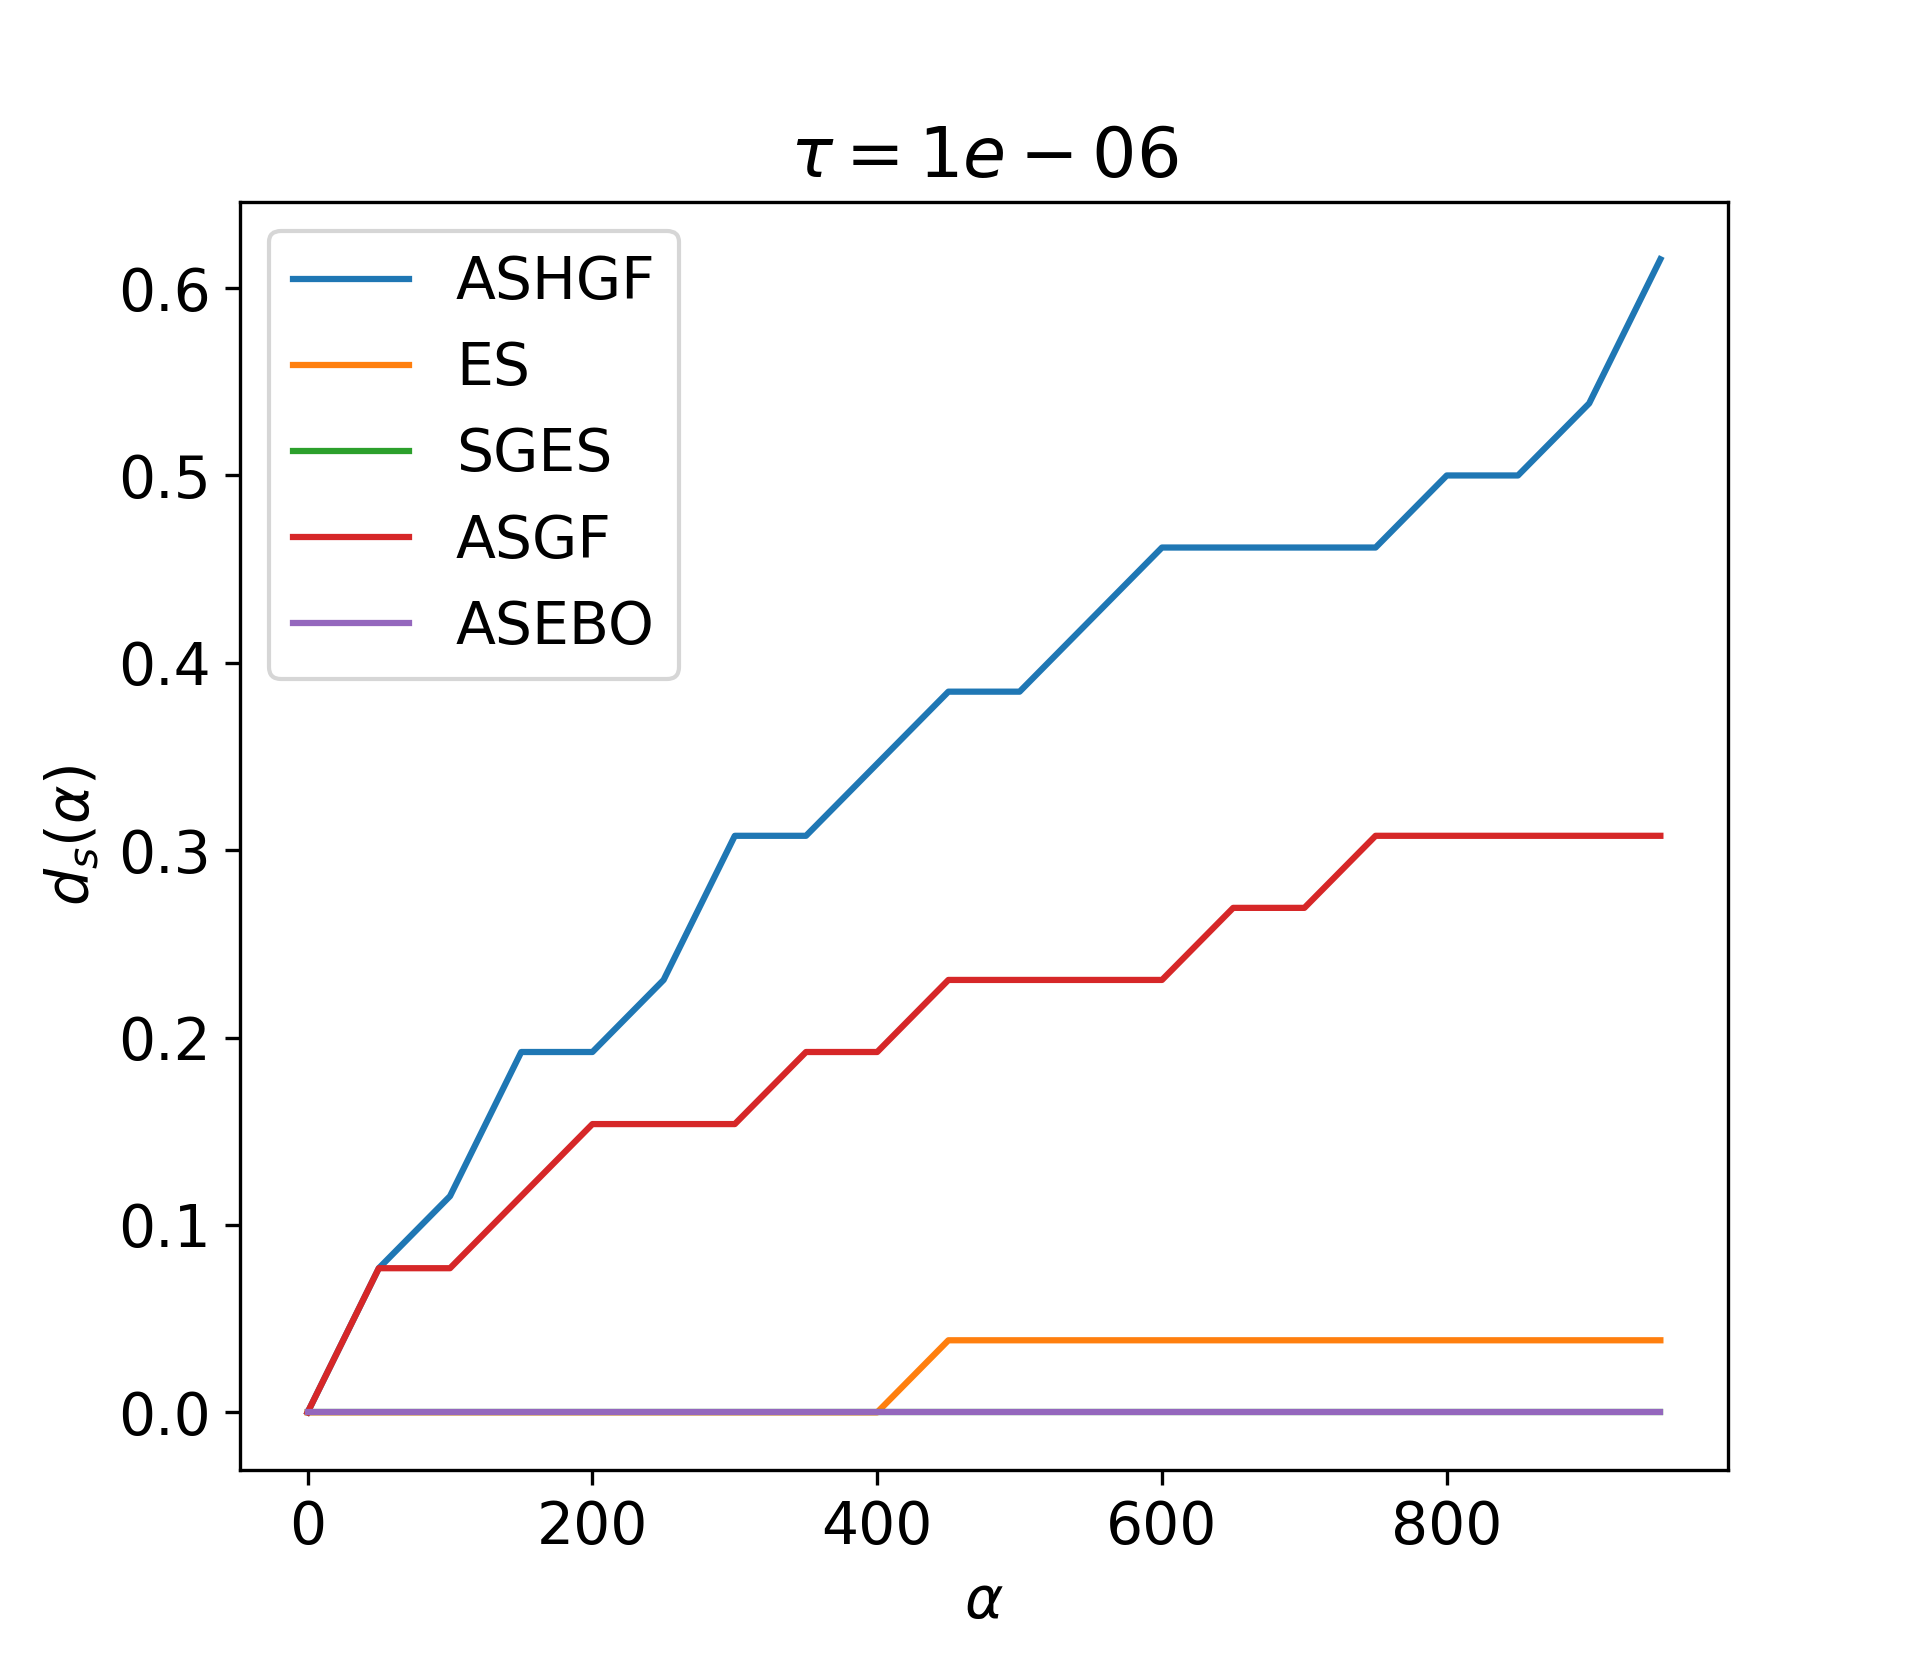
\includegraphics[width=1\textwidth]{figures/data_profiles/100/data_profile_100_100000_1e-06.png}
\end{subfigure}
\centering
\begin{subfigure}{0.3\textwidth}
  \centering 
  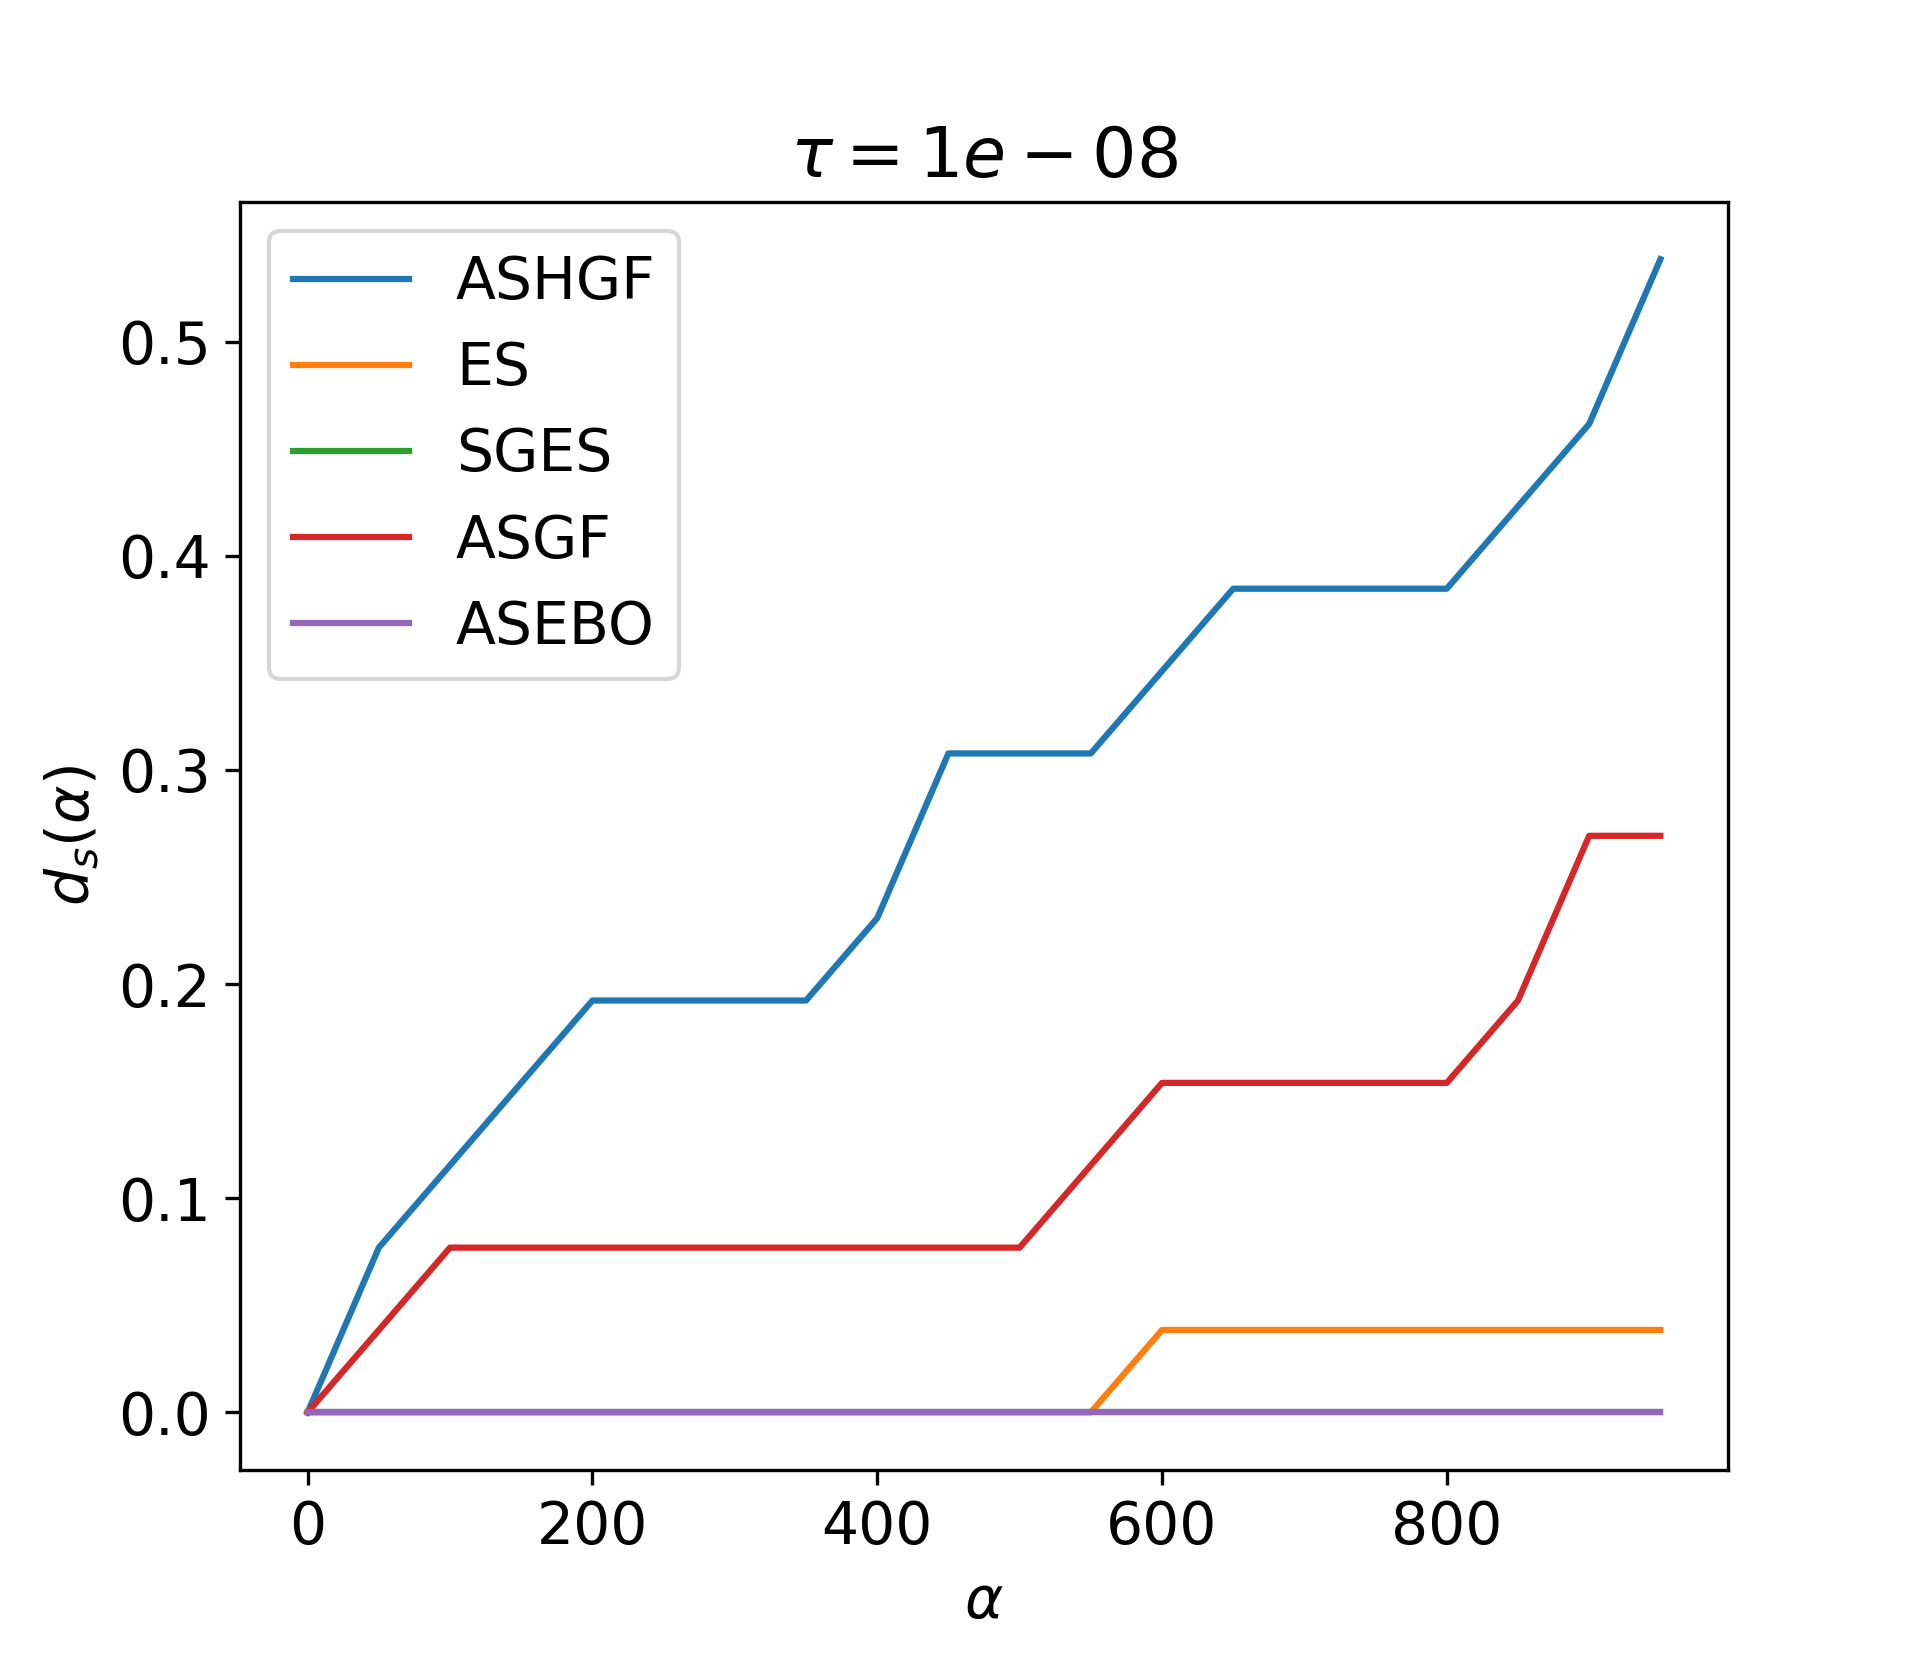
\includegraphics[width=1\textwidth]{figures/data_profiles/100/data_profile_100_100000_1e-08.png}
\end{subfigure}%
\begin{subfigure}{0.3\textwidth}
  \centering 
  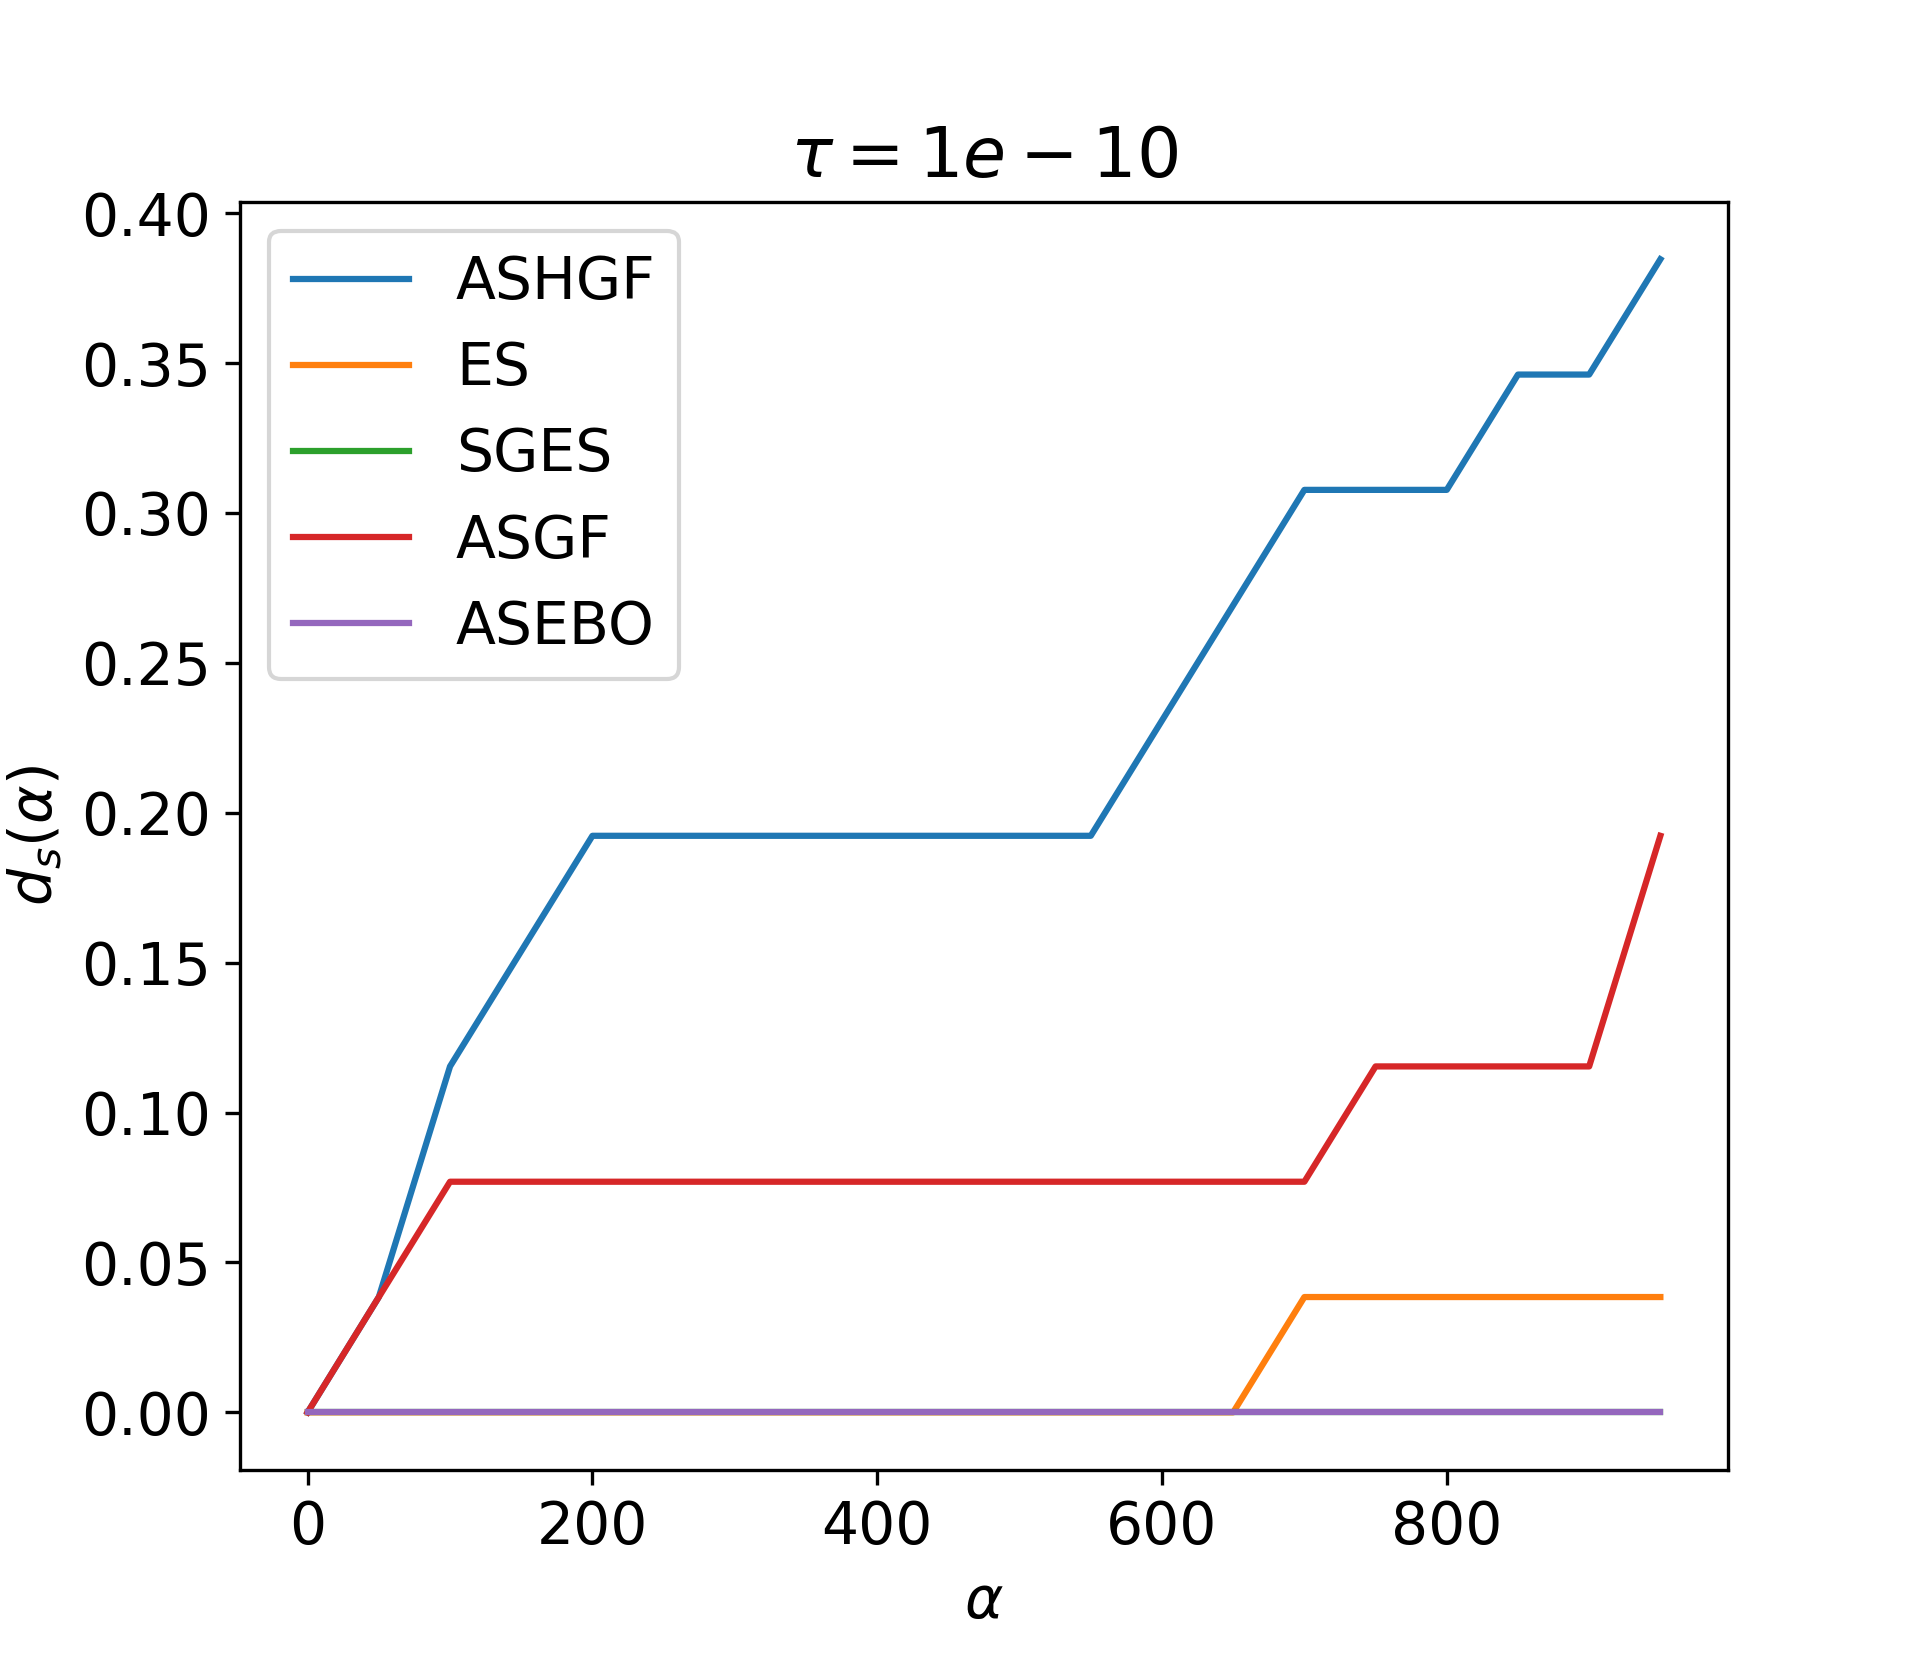
\includegraphics[width=1\textwidth]{figures/data_profiles/100/data_profile_100_100000_1e-10.png}
\end{subfigure}
\caption{Data profiles with $\mu_L = 10^{5}$}
\label{DataProfiles100Mu100000}
\end{figure}

\begin{figure}[H]
\centering
\begin{subfigure}{0.3\textwidth}
  \centering 
  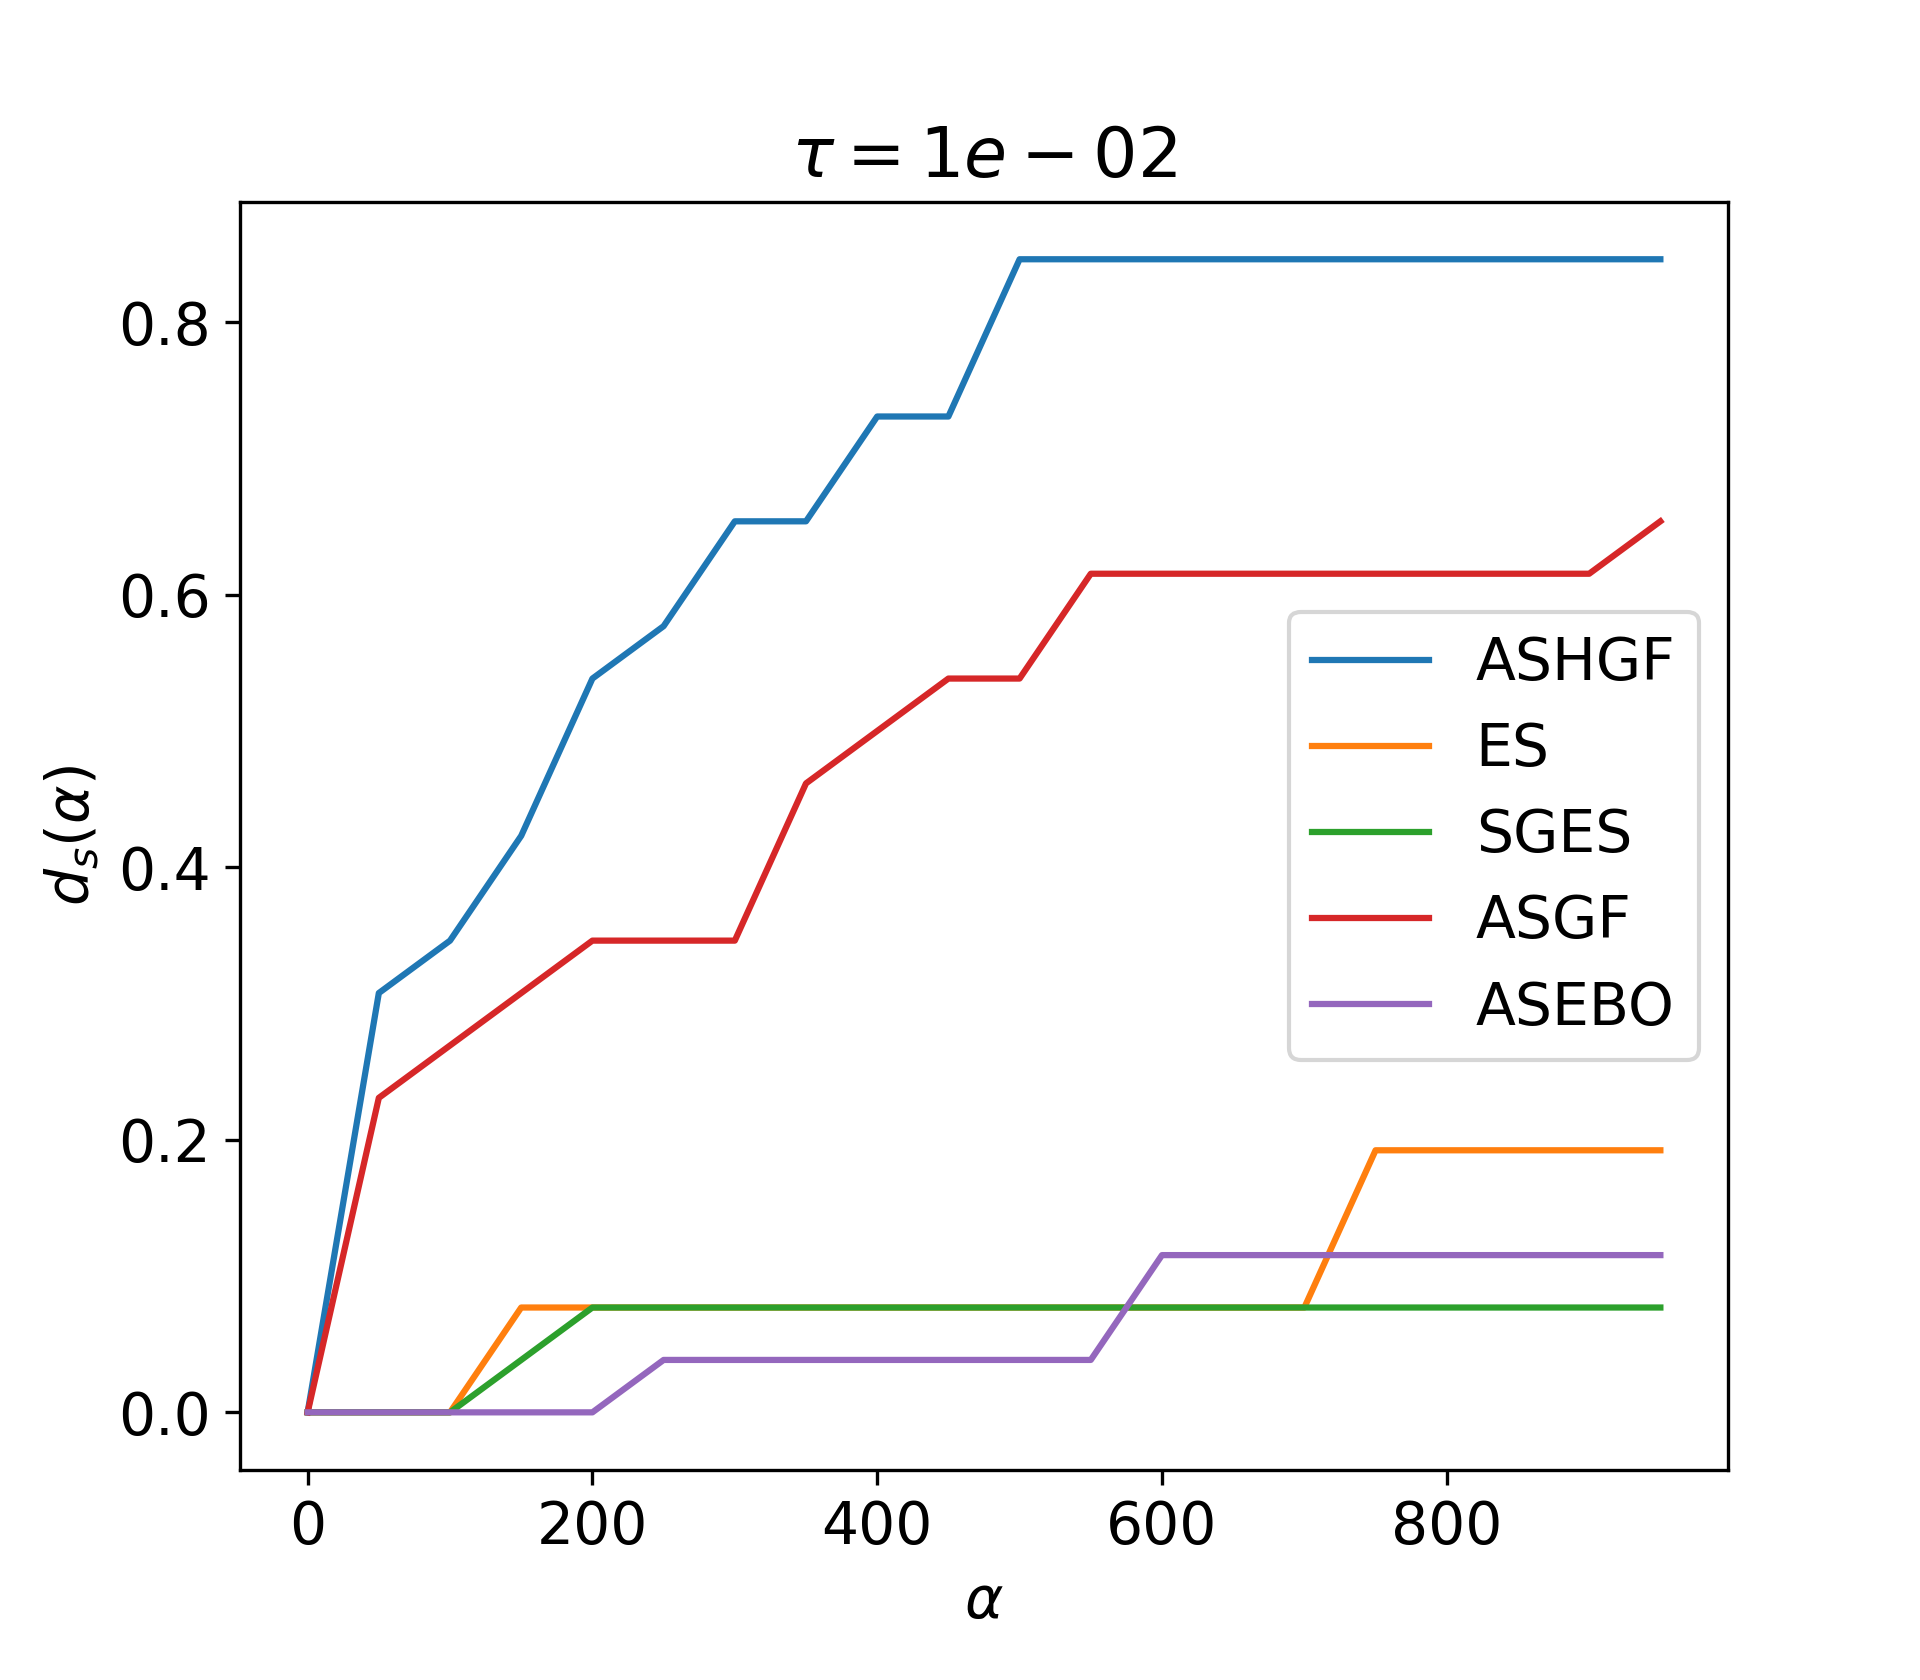
\includegraphics[width=1\textwidth]{figures/data_profiles/100/data_profile_100_1000000_1e-02.png}
\end{subfigure}%
\begin{subfigure}{0.3\textwidth}
  \centering 
  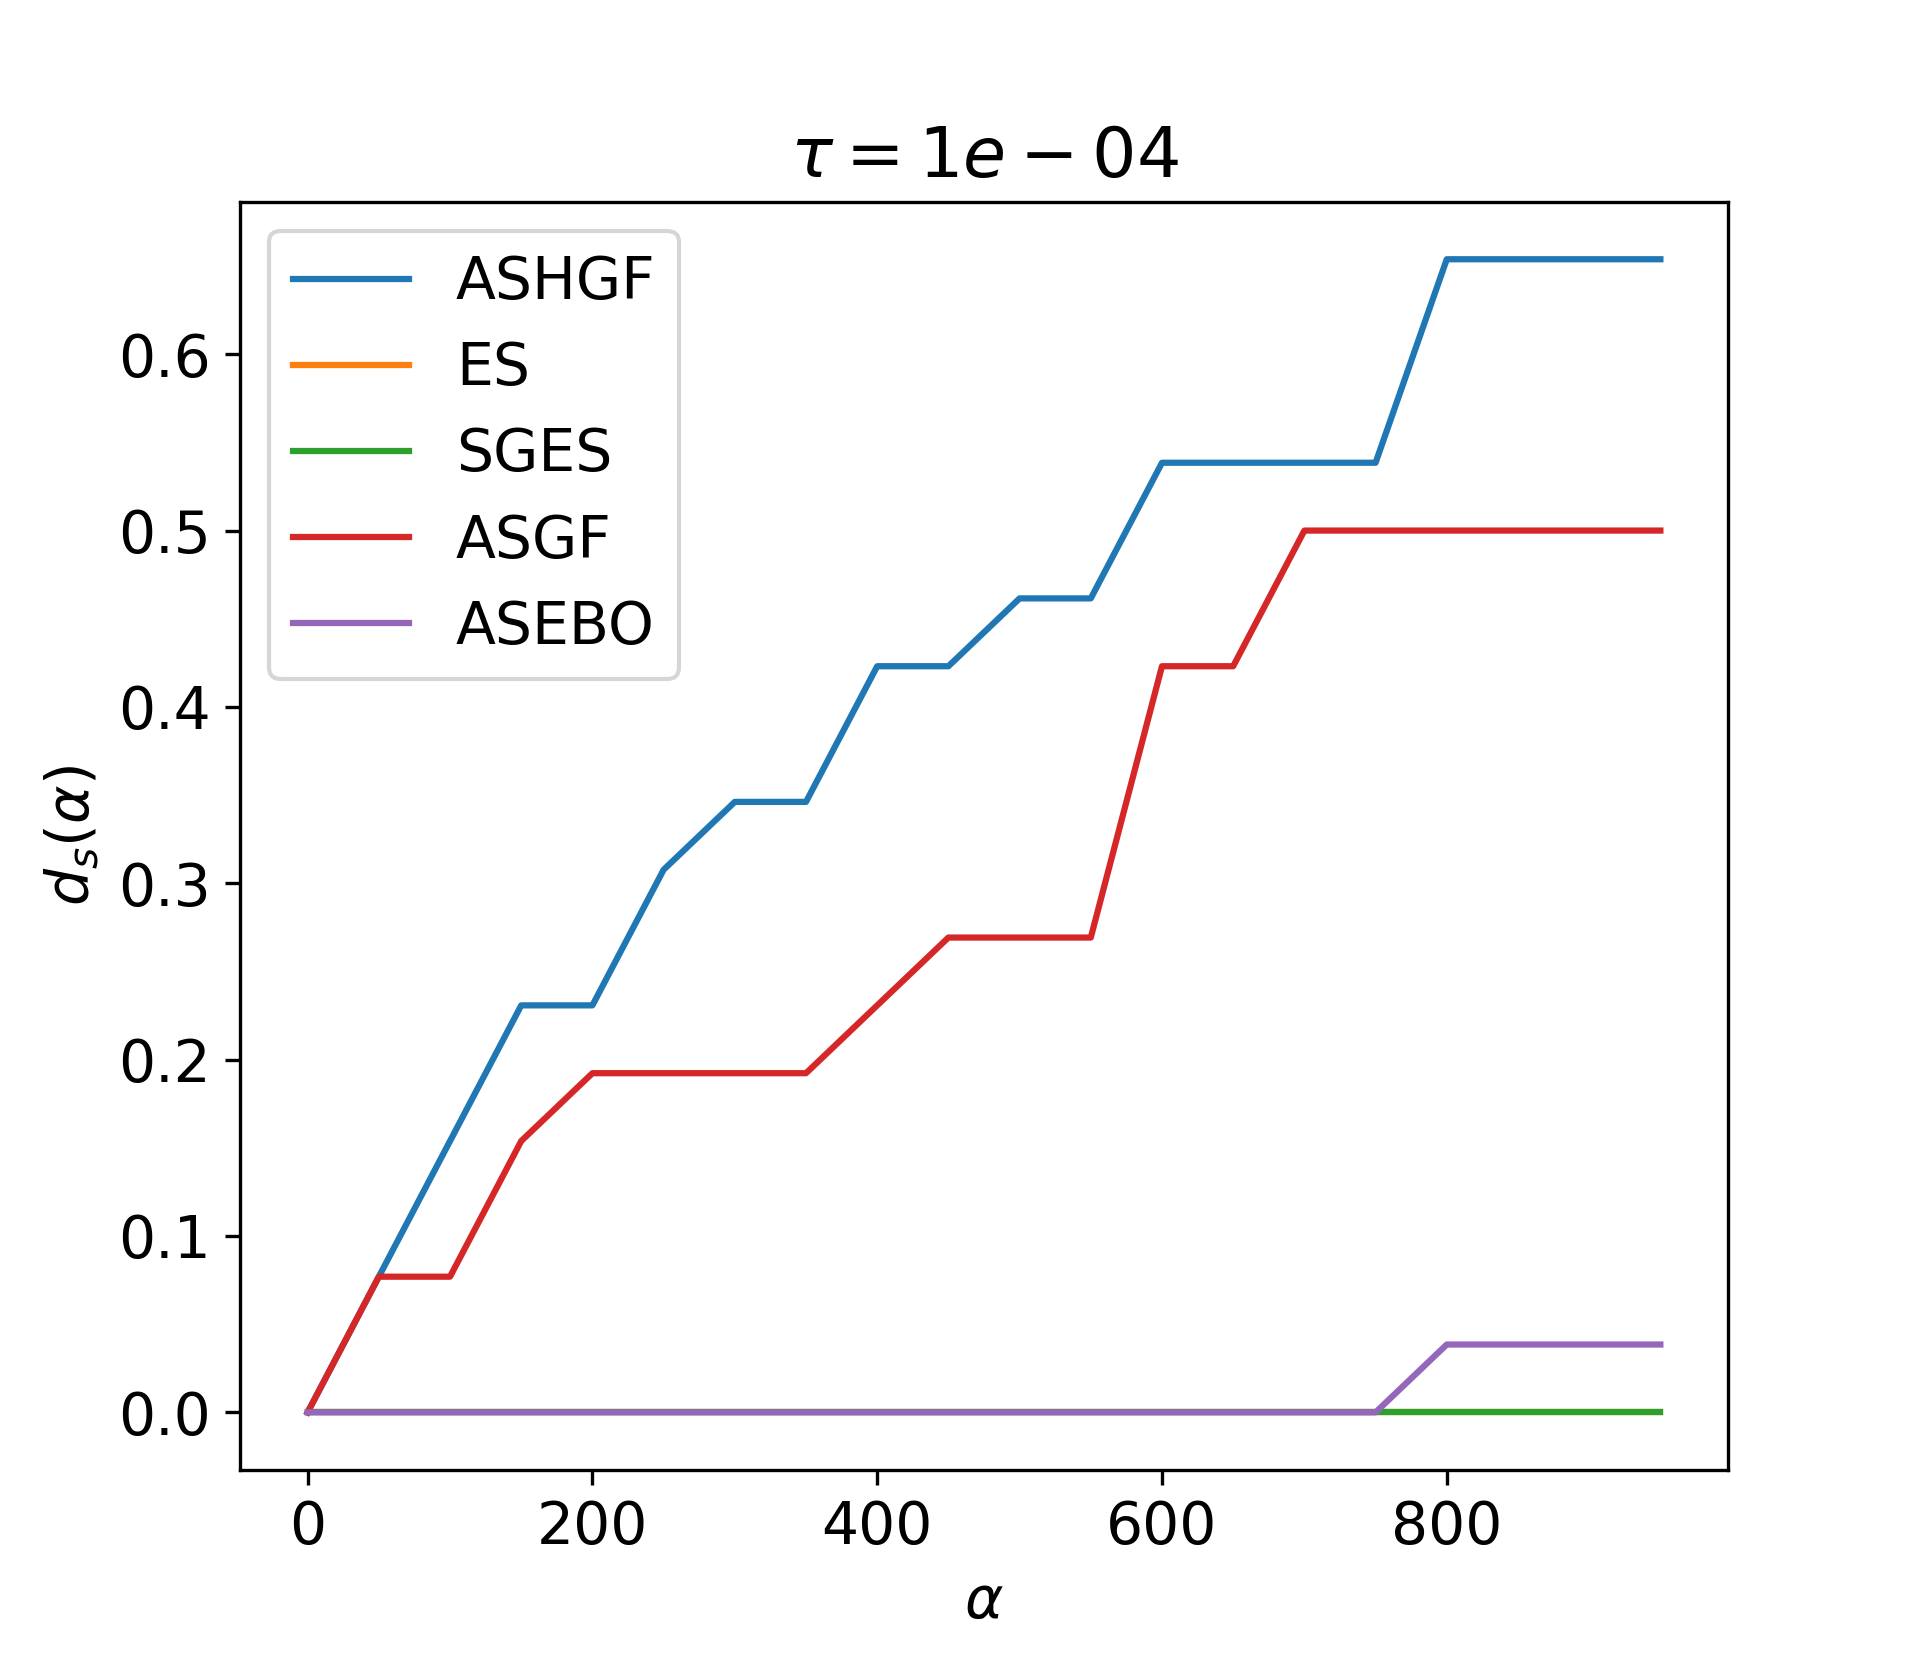
\includegraphics[width=1\textwidth]{figures/data_profiles/100/data_profile_100_1000000_1e-04.png}
\end{subfigure}
\begin{subfigure}{0.3\textwidth}
  \centering 
  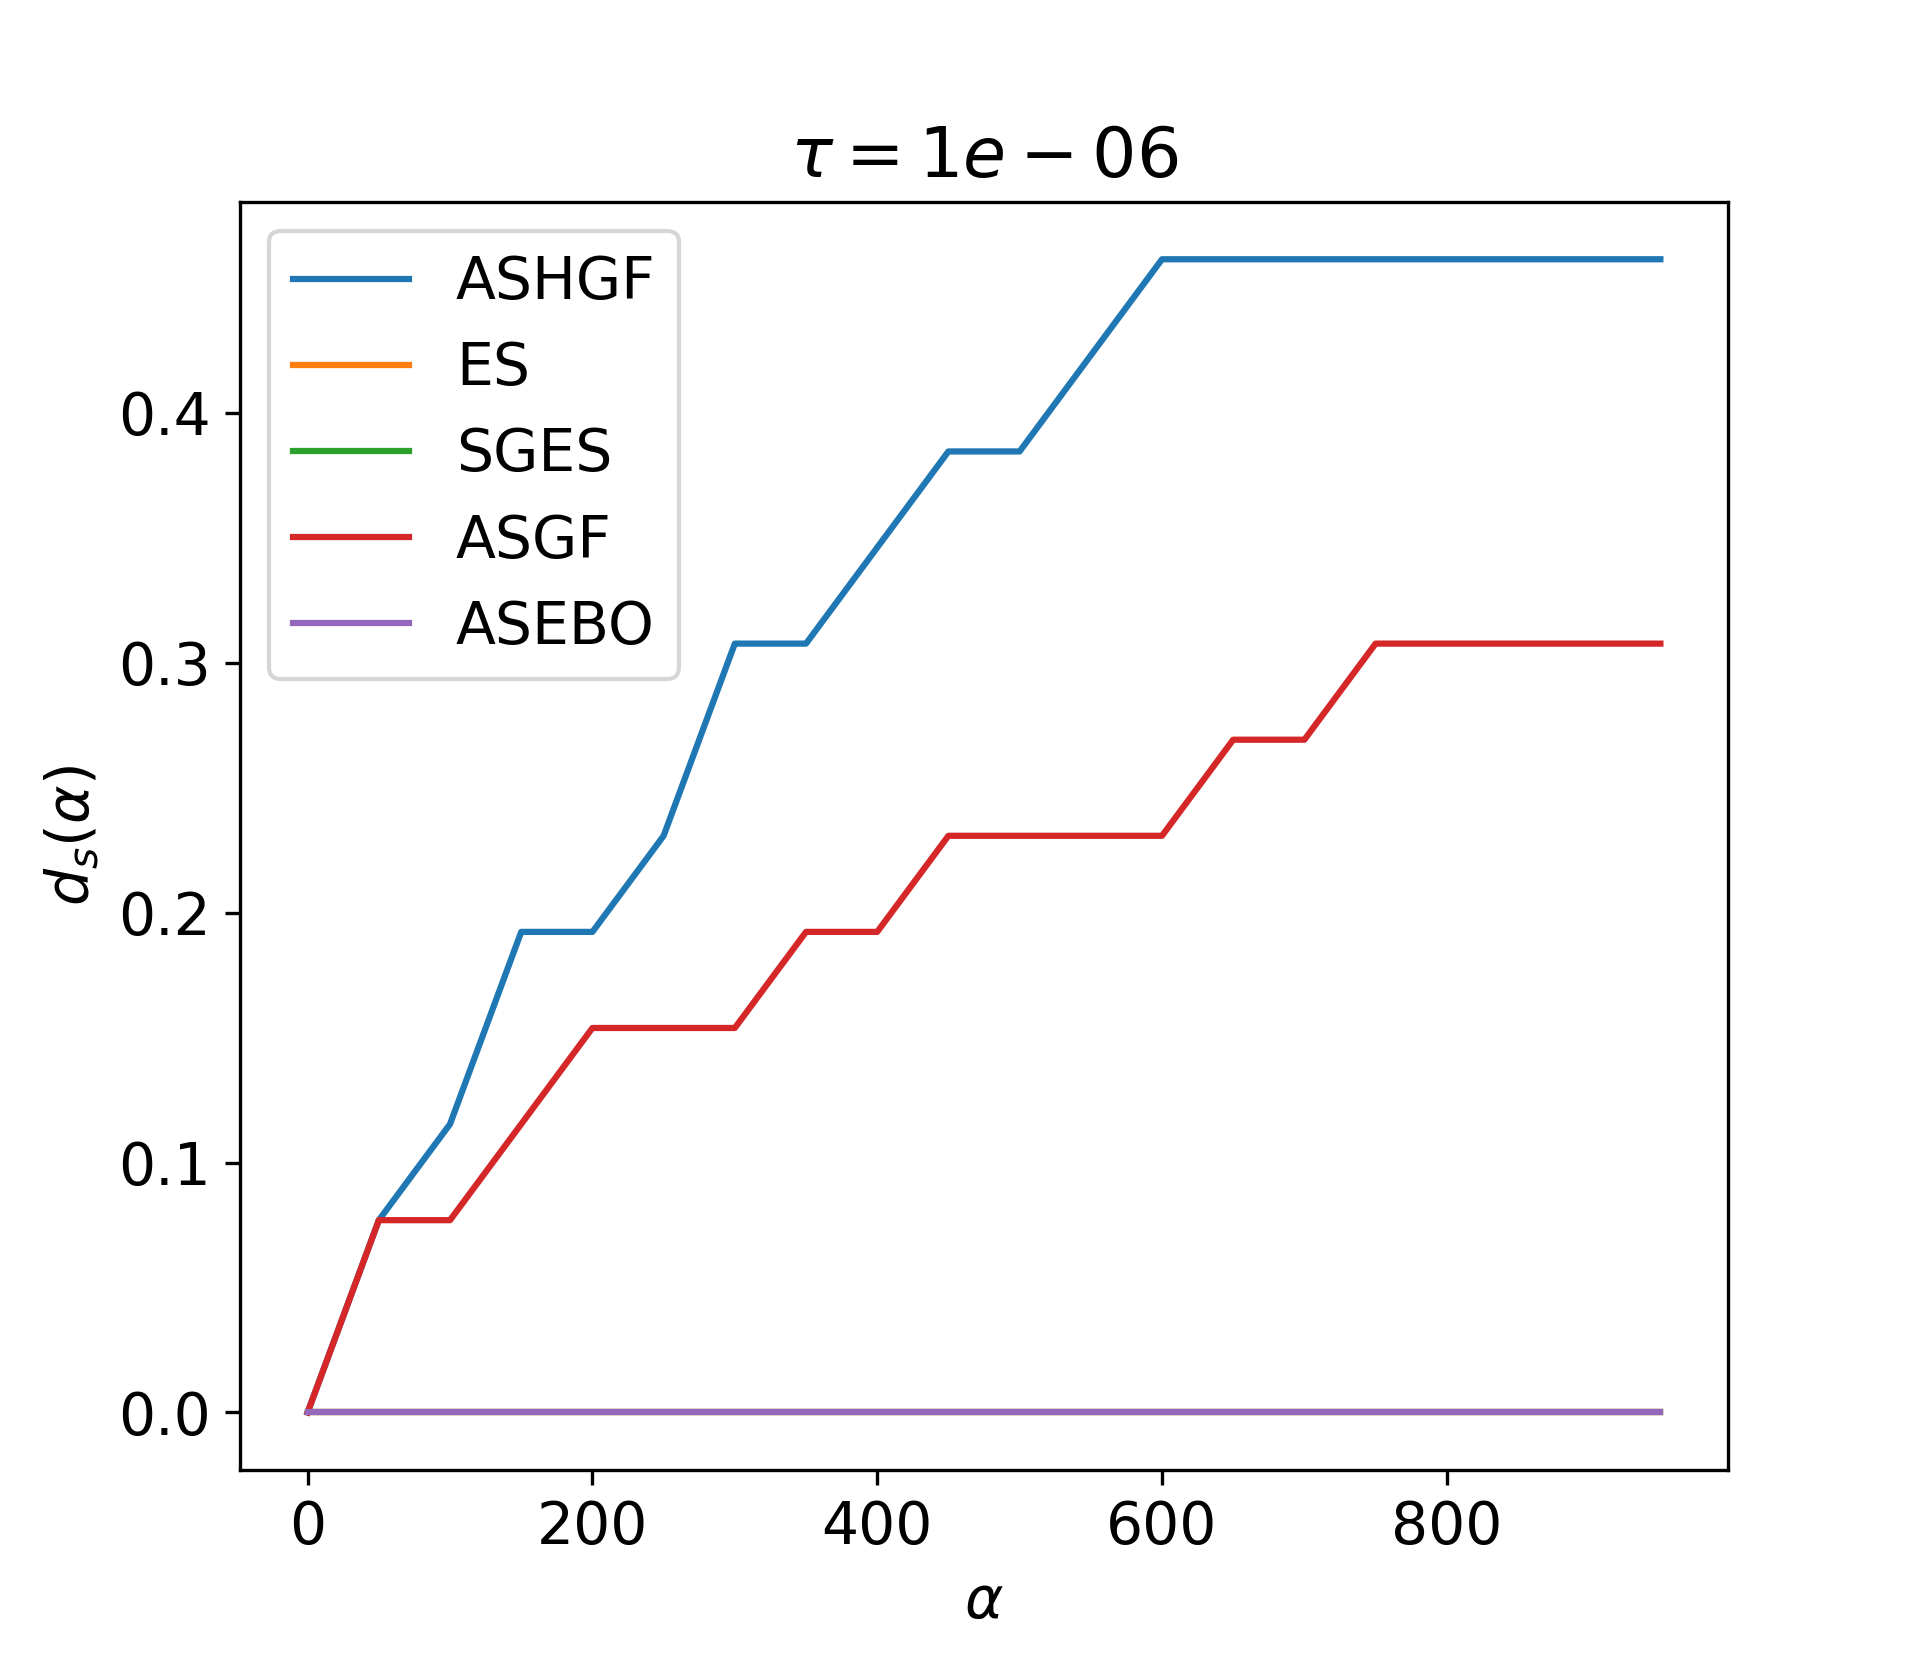
\includegraphics[width=1\textwidth]{figures/data_profiles/100/data_profile_100_1000000_1e-06.png}
\end{subfigure}
\centering
\begin{subfigure}{0.3\textwidth}
  \centering 
  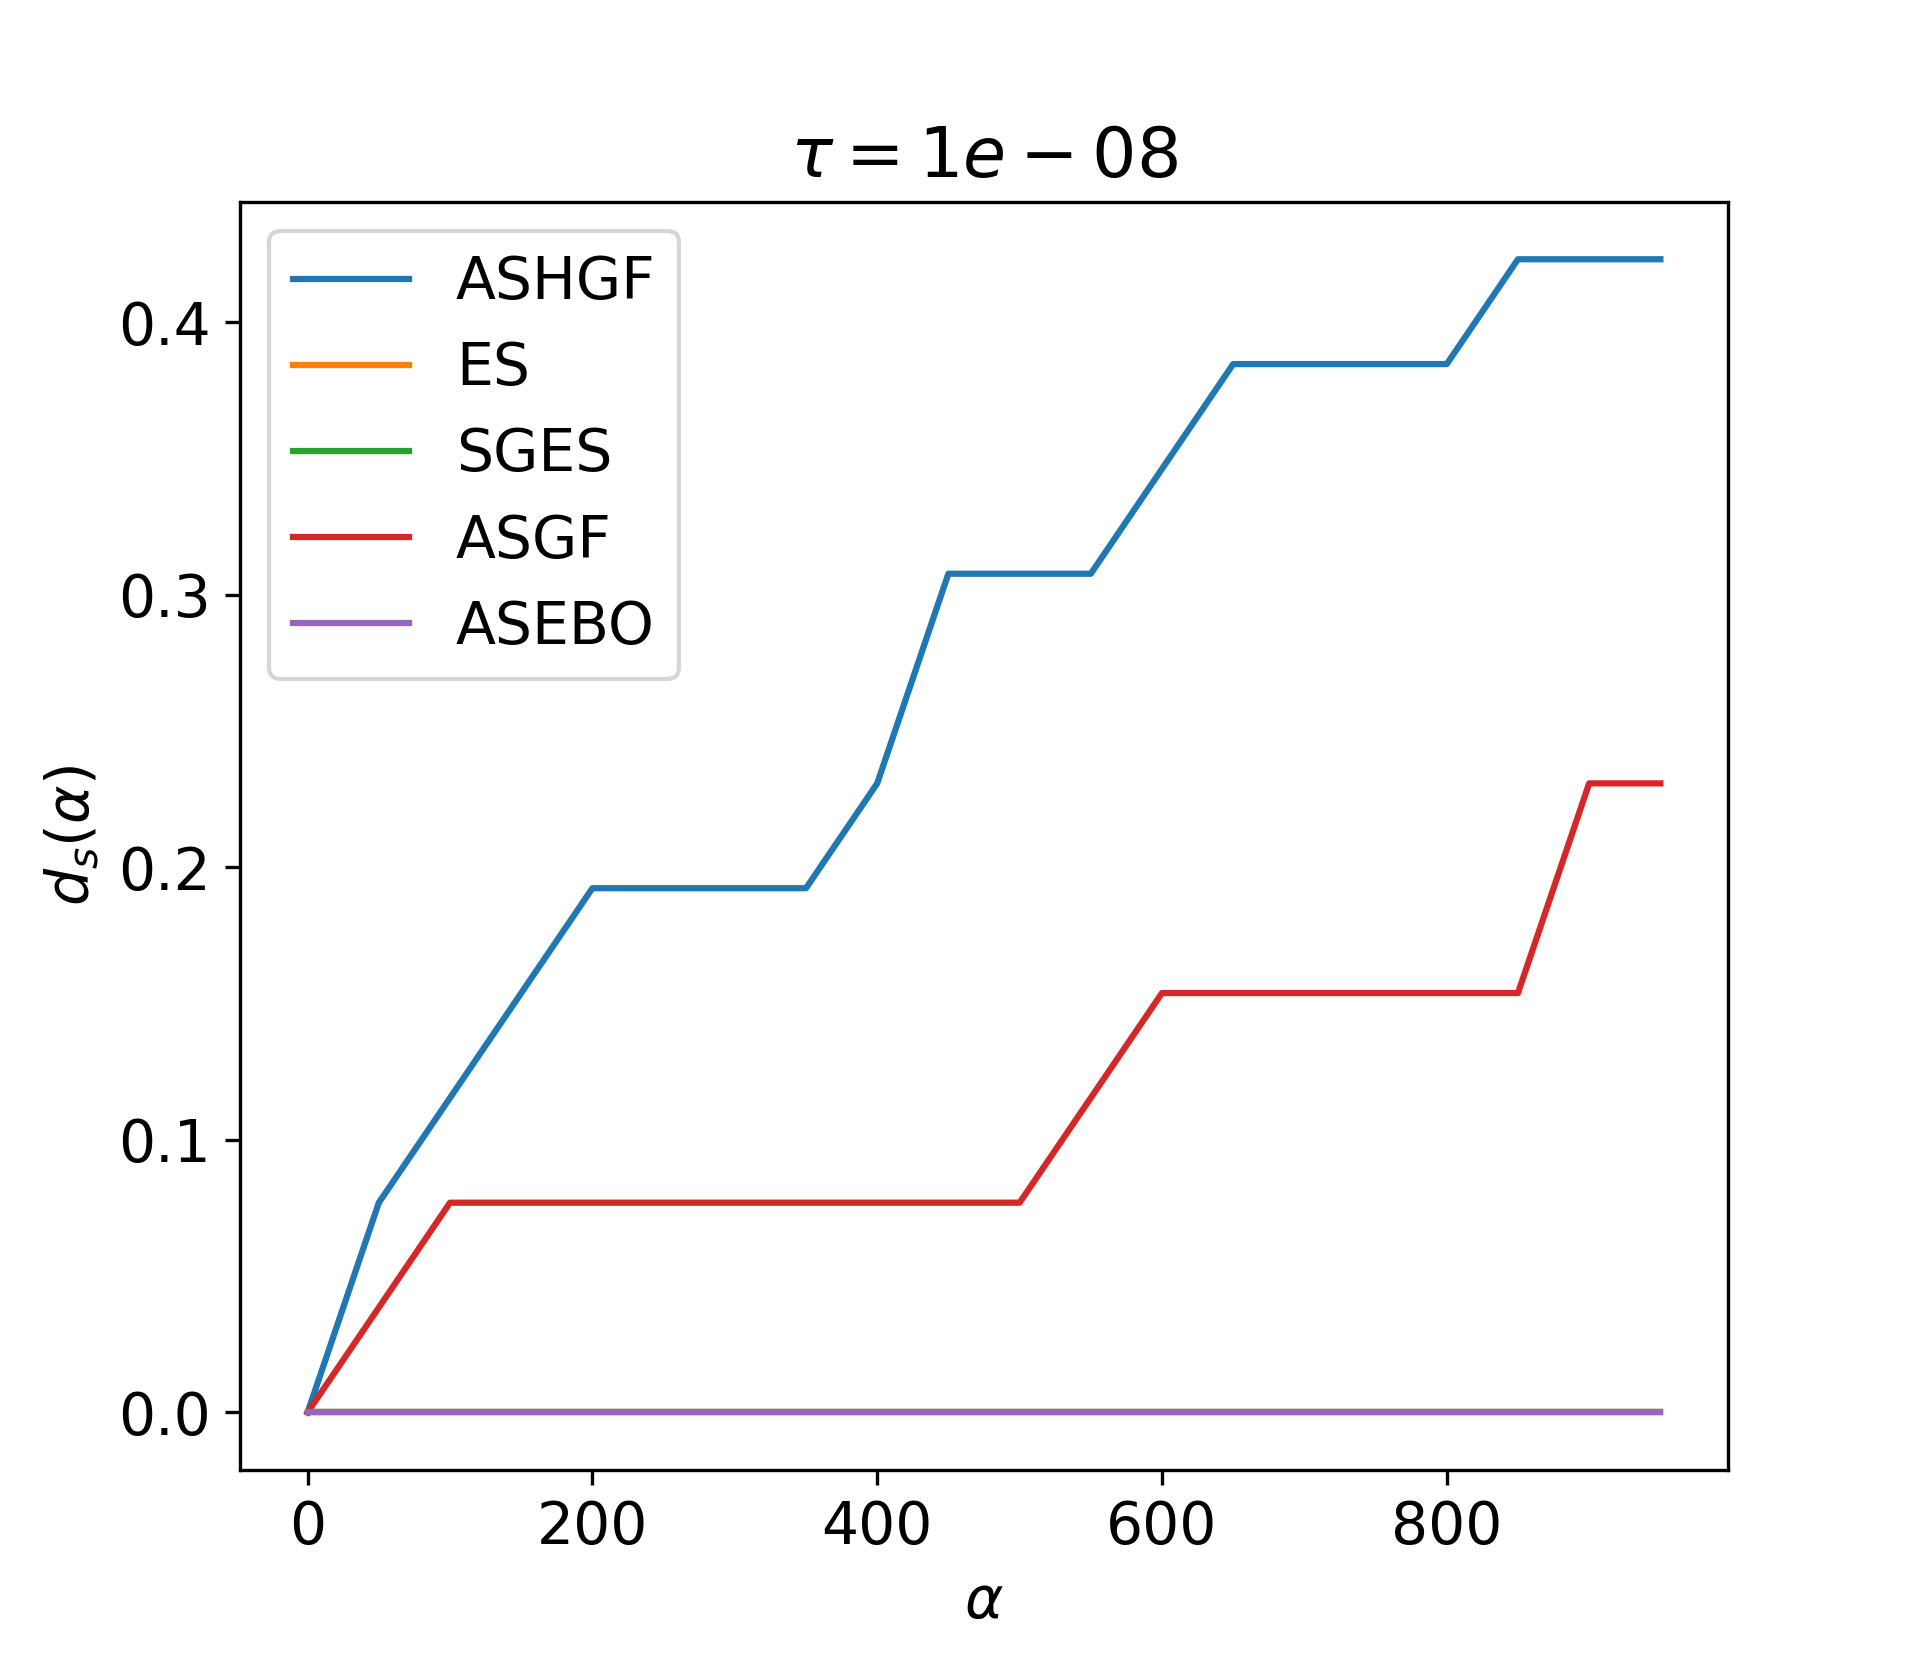
\includegraphics[width=1\textwidth]{figures/data_profiles/100/data_profile_100_1000000_1e-08.png}
\end{subfigure}%
\begin{subfigure}{0.3\textwidth}
  \centering 
  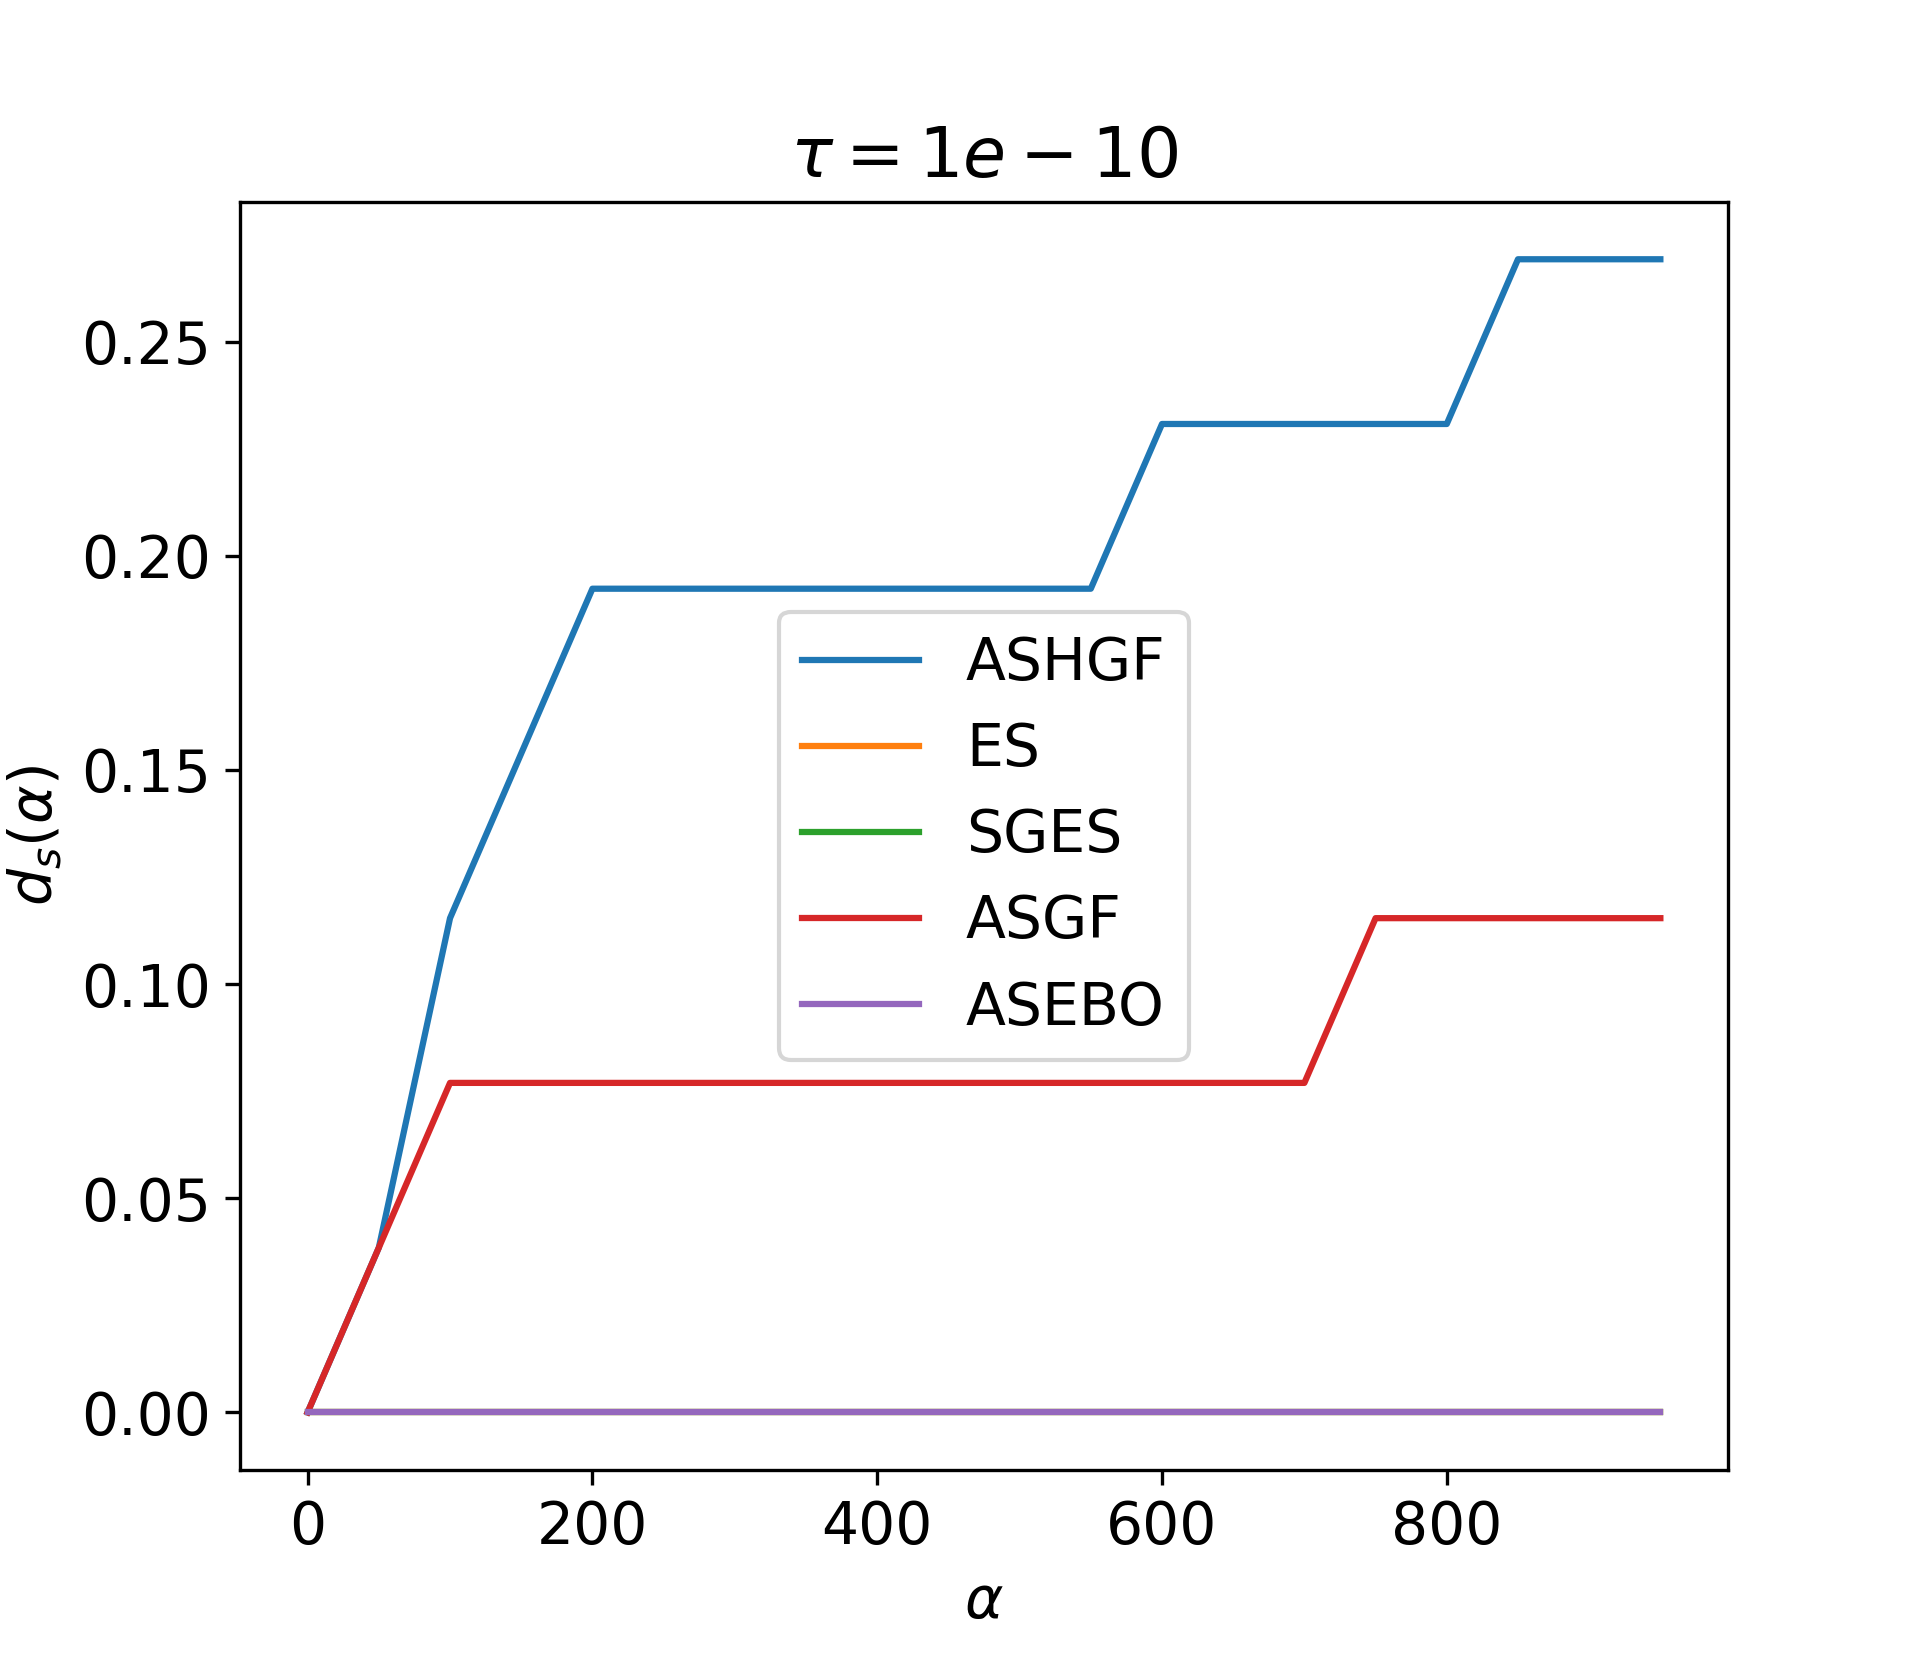
\includegraphics[width=1\textwidth]{figures/data_profiles/100/data_profile_100_1000000_1e-10.png}
\end{subfigure}
\caption{Data profiles with $\mu_L = 10^{6}$}
\label{DataProfiles100Mu1000000}
\end{figure}

\begin{figure}[H]
\centering
\begin{subfigure}{0.3\textwidth}
  \centering 
  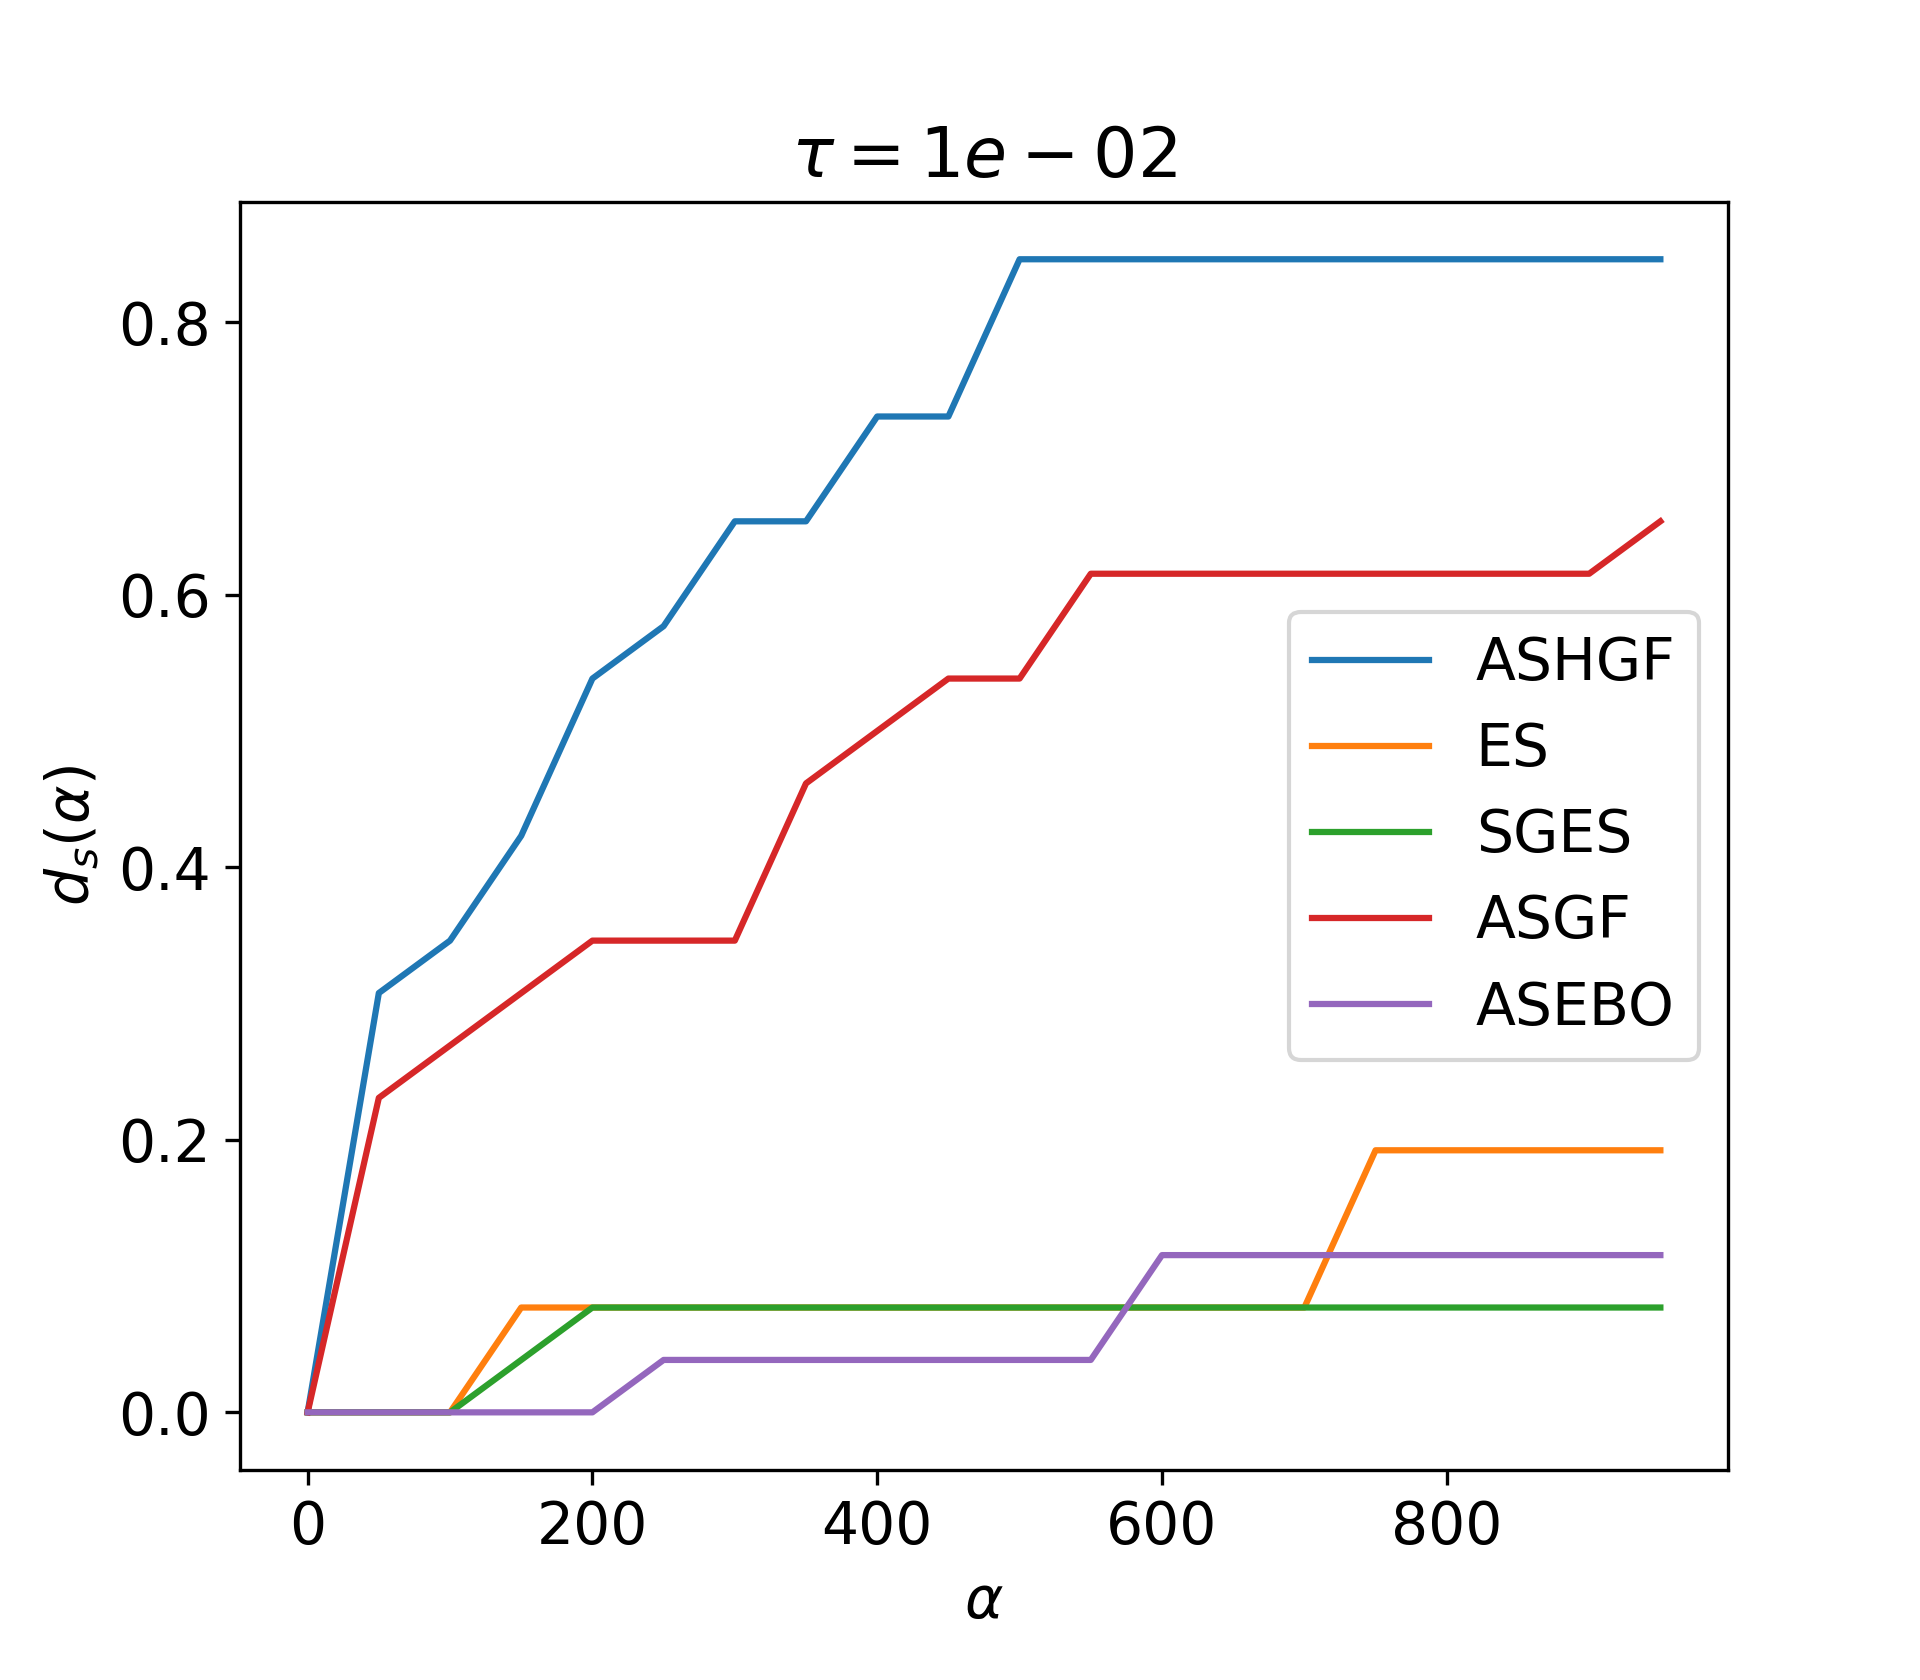
\includegraphics[width=1\textwidth]{figures/data_profiles/100/data_profile_100_10000000_1e-02.png}
\end{subfigure}%
\begin{subfigure}{0.3\textwidth}
  \centering 
  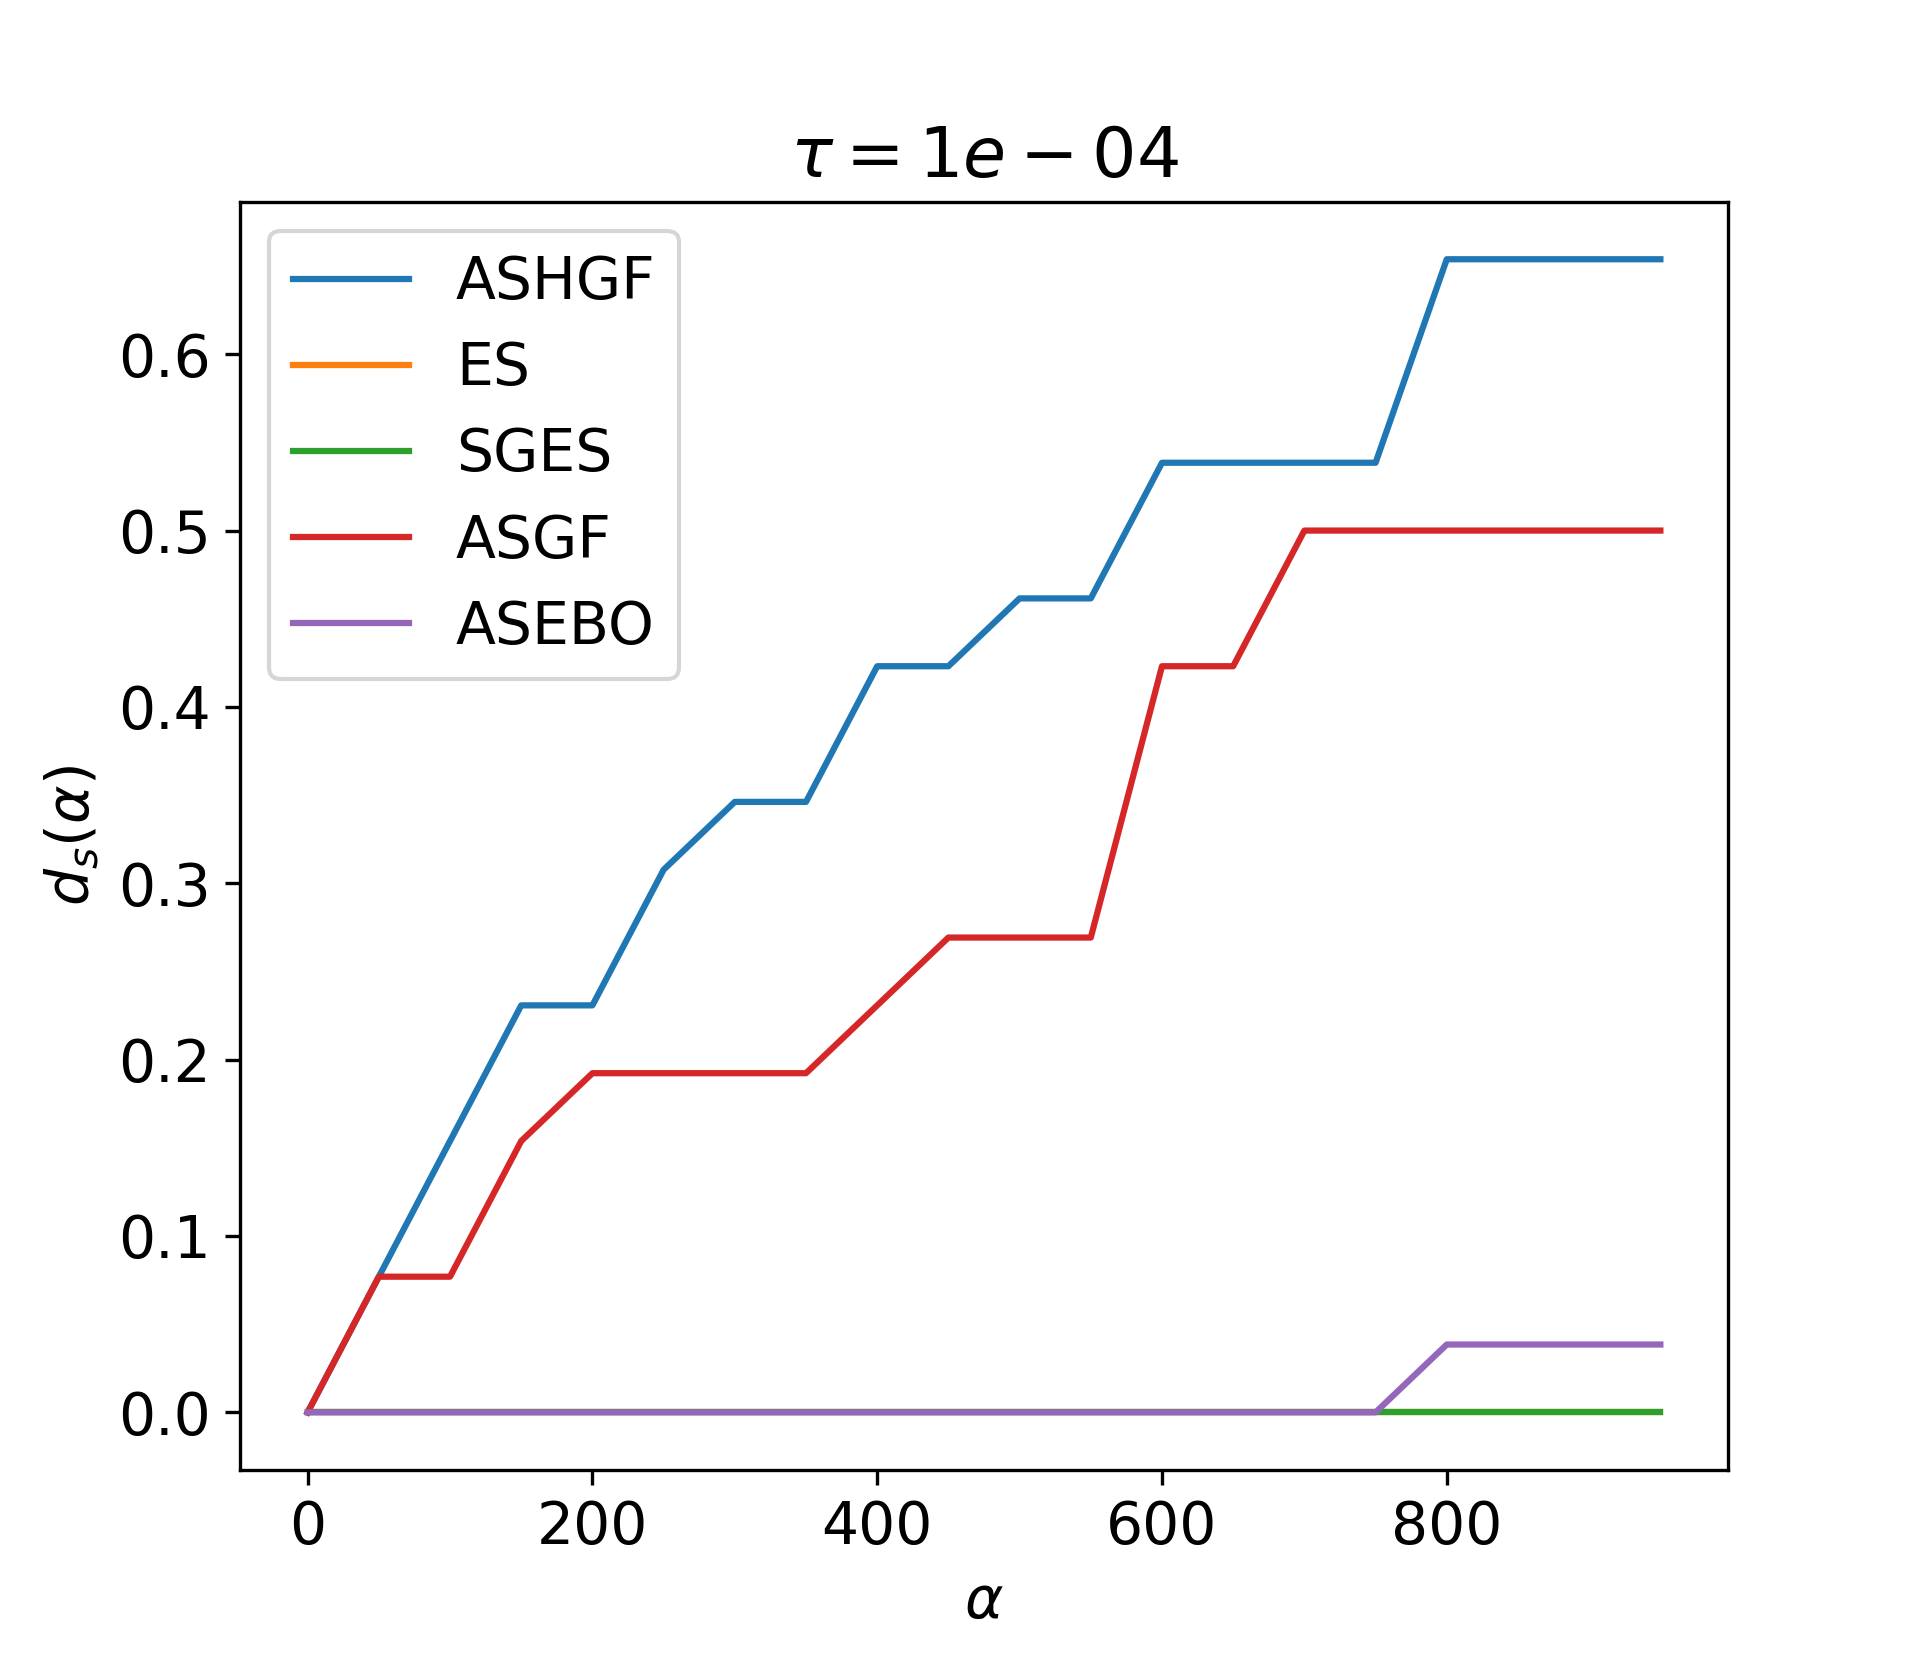
\includegraphics[width=1\textwidth]{figures/data_profiles/100/data_profile_100_10000000_1e-04.png}
\end{subfigure}
\begin{subfigure}{0.3\textwidth}
  \centering 
  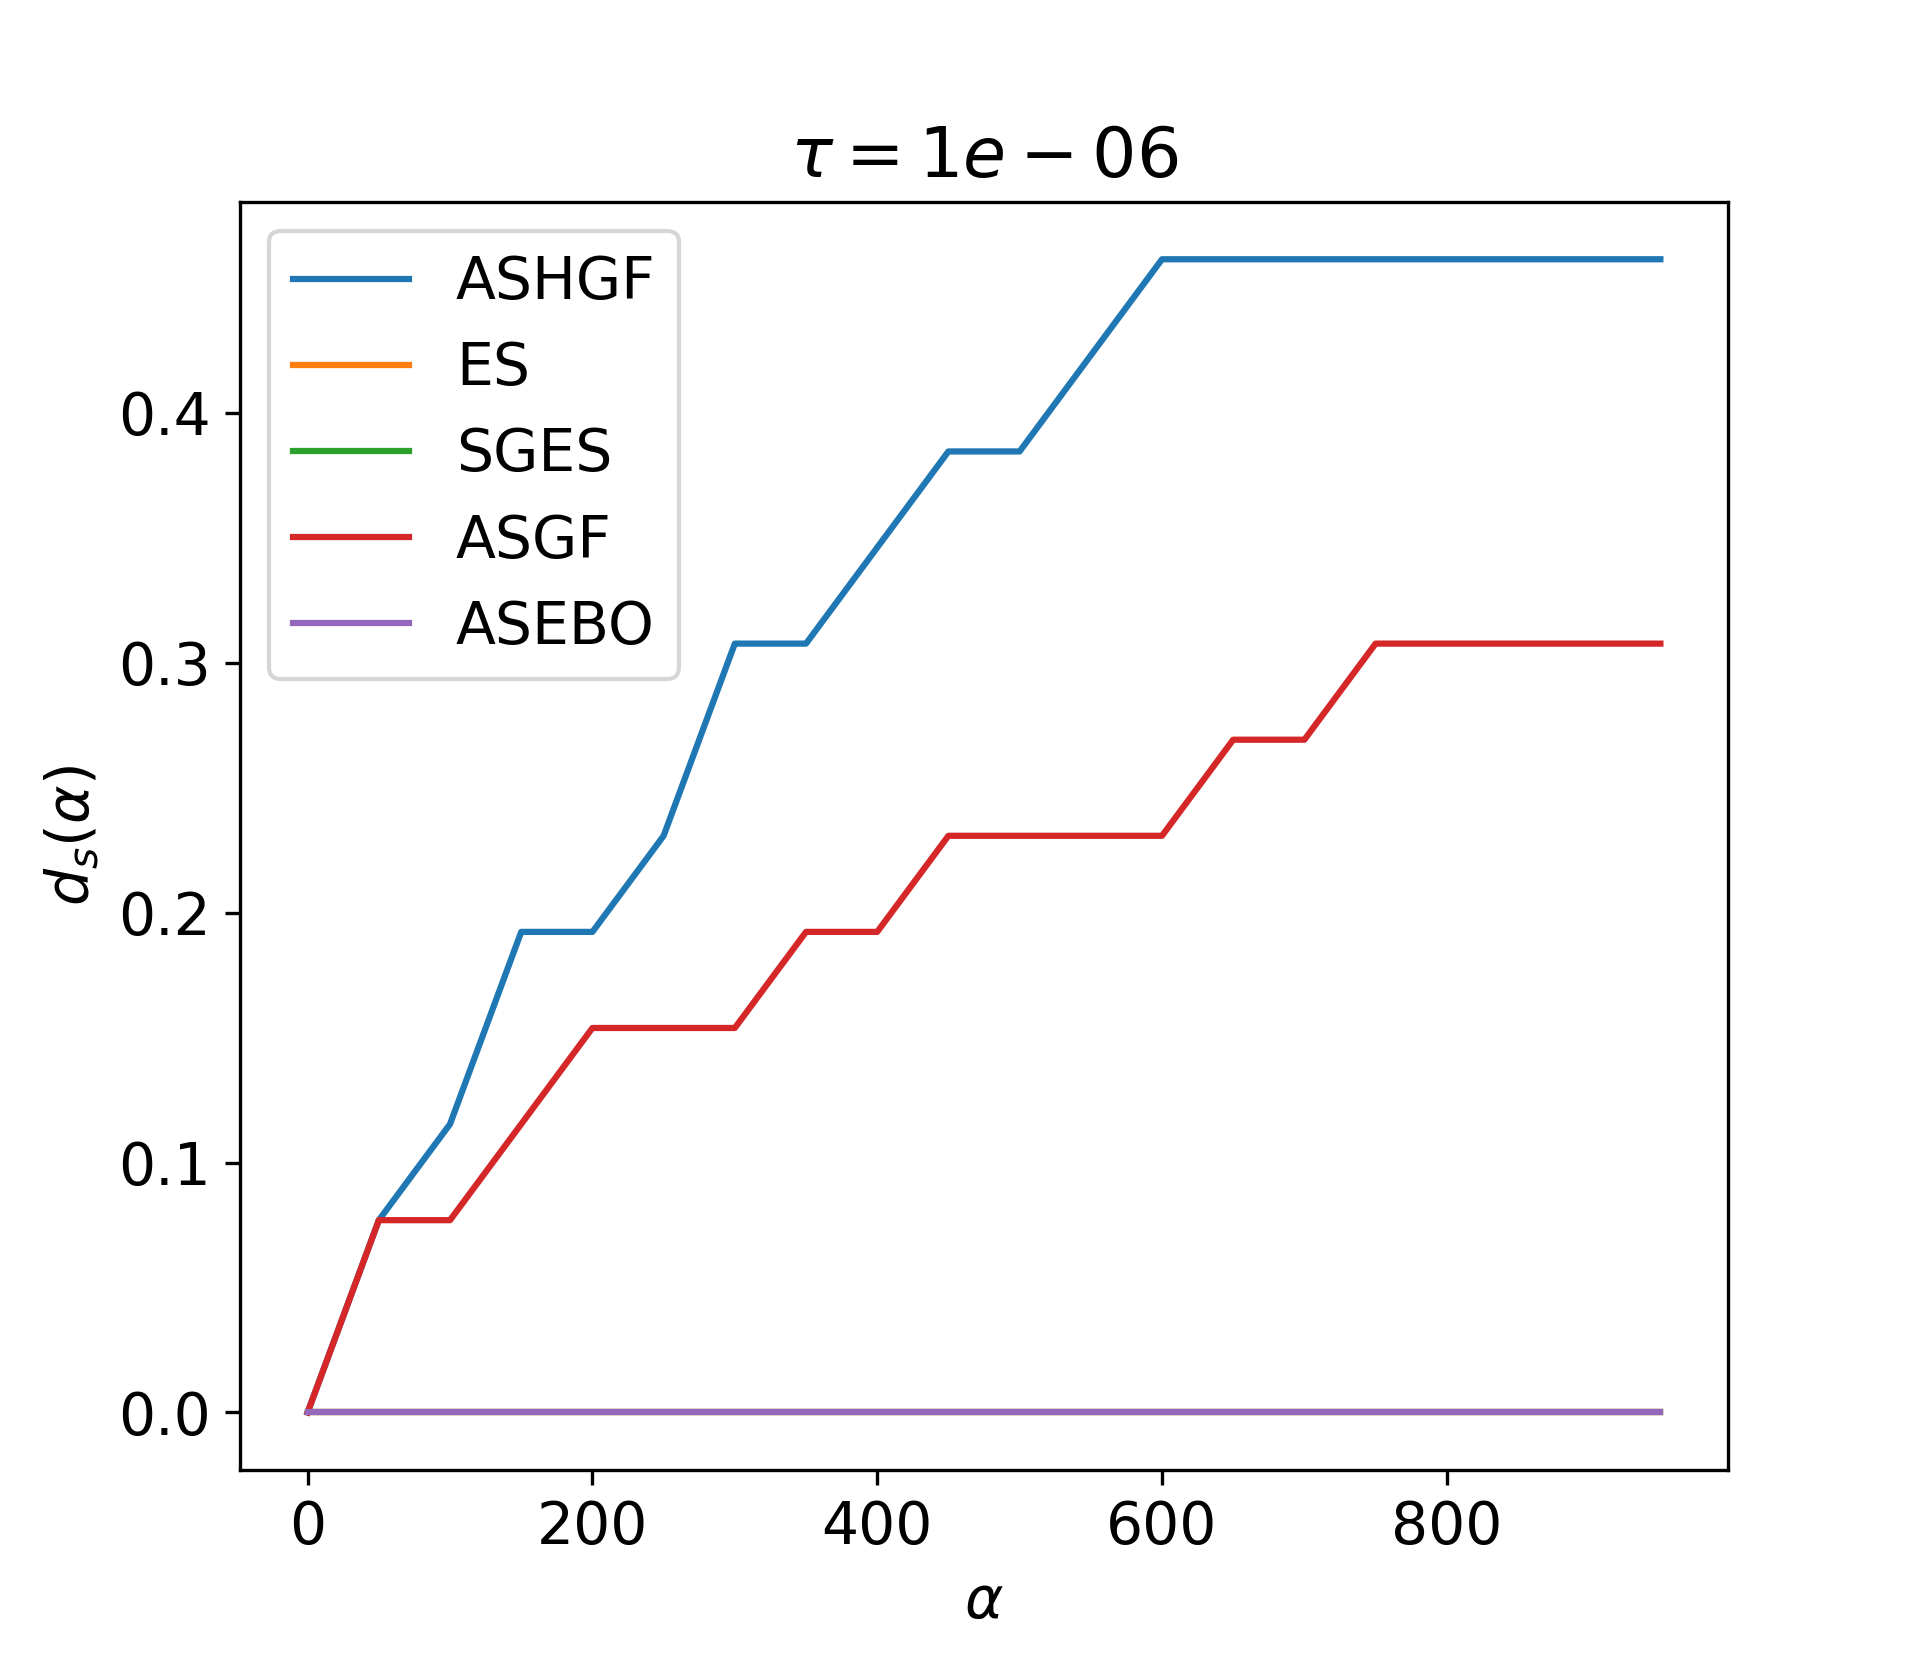
\includegraphics[width=1\textwidth]{figures/data_profiles/100/data_profile_100_10000000_1e-06.png}
\end{subfigure}
\centering
\begin{subfigure}{0.3\textwidth}
  \centering 
  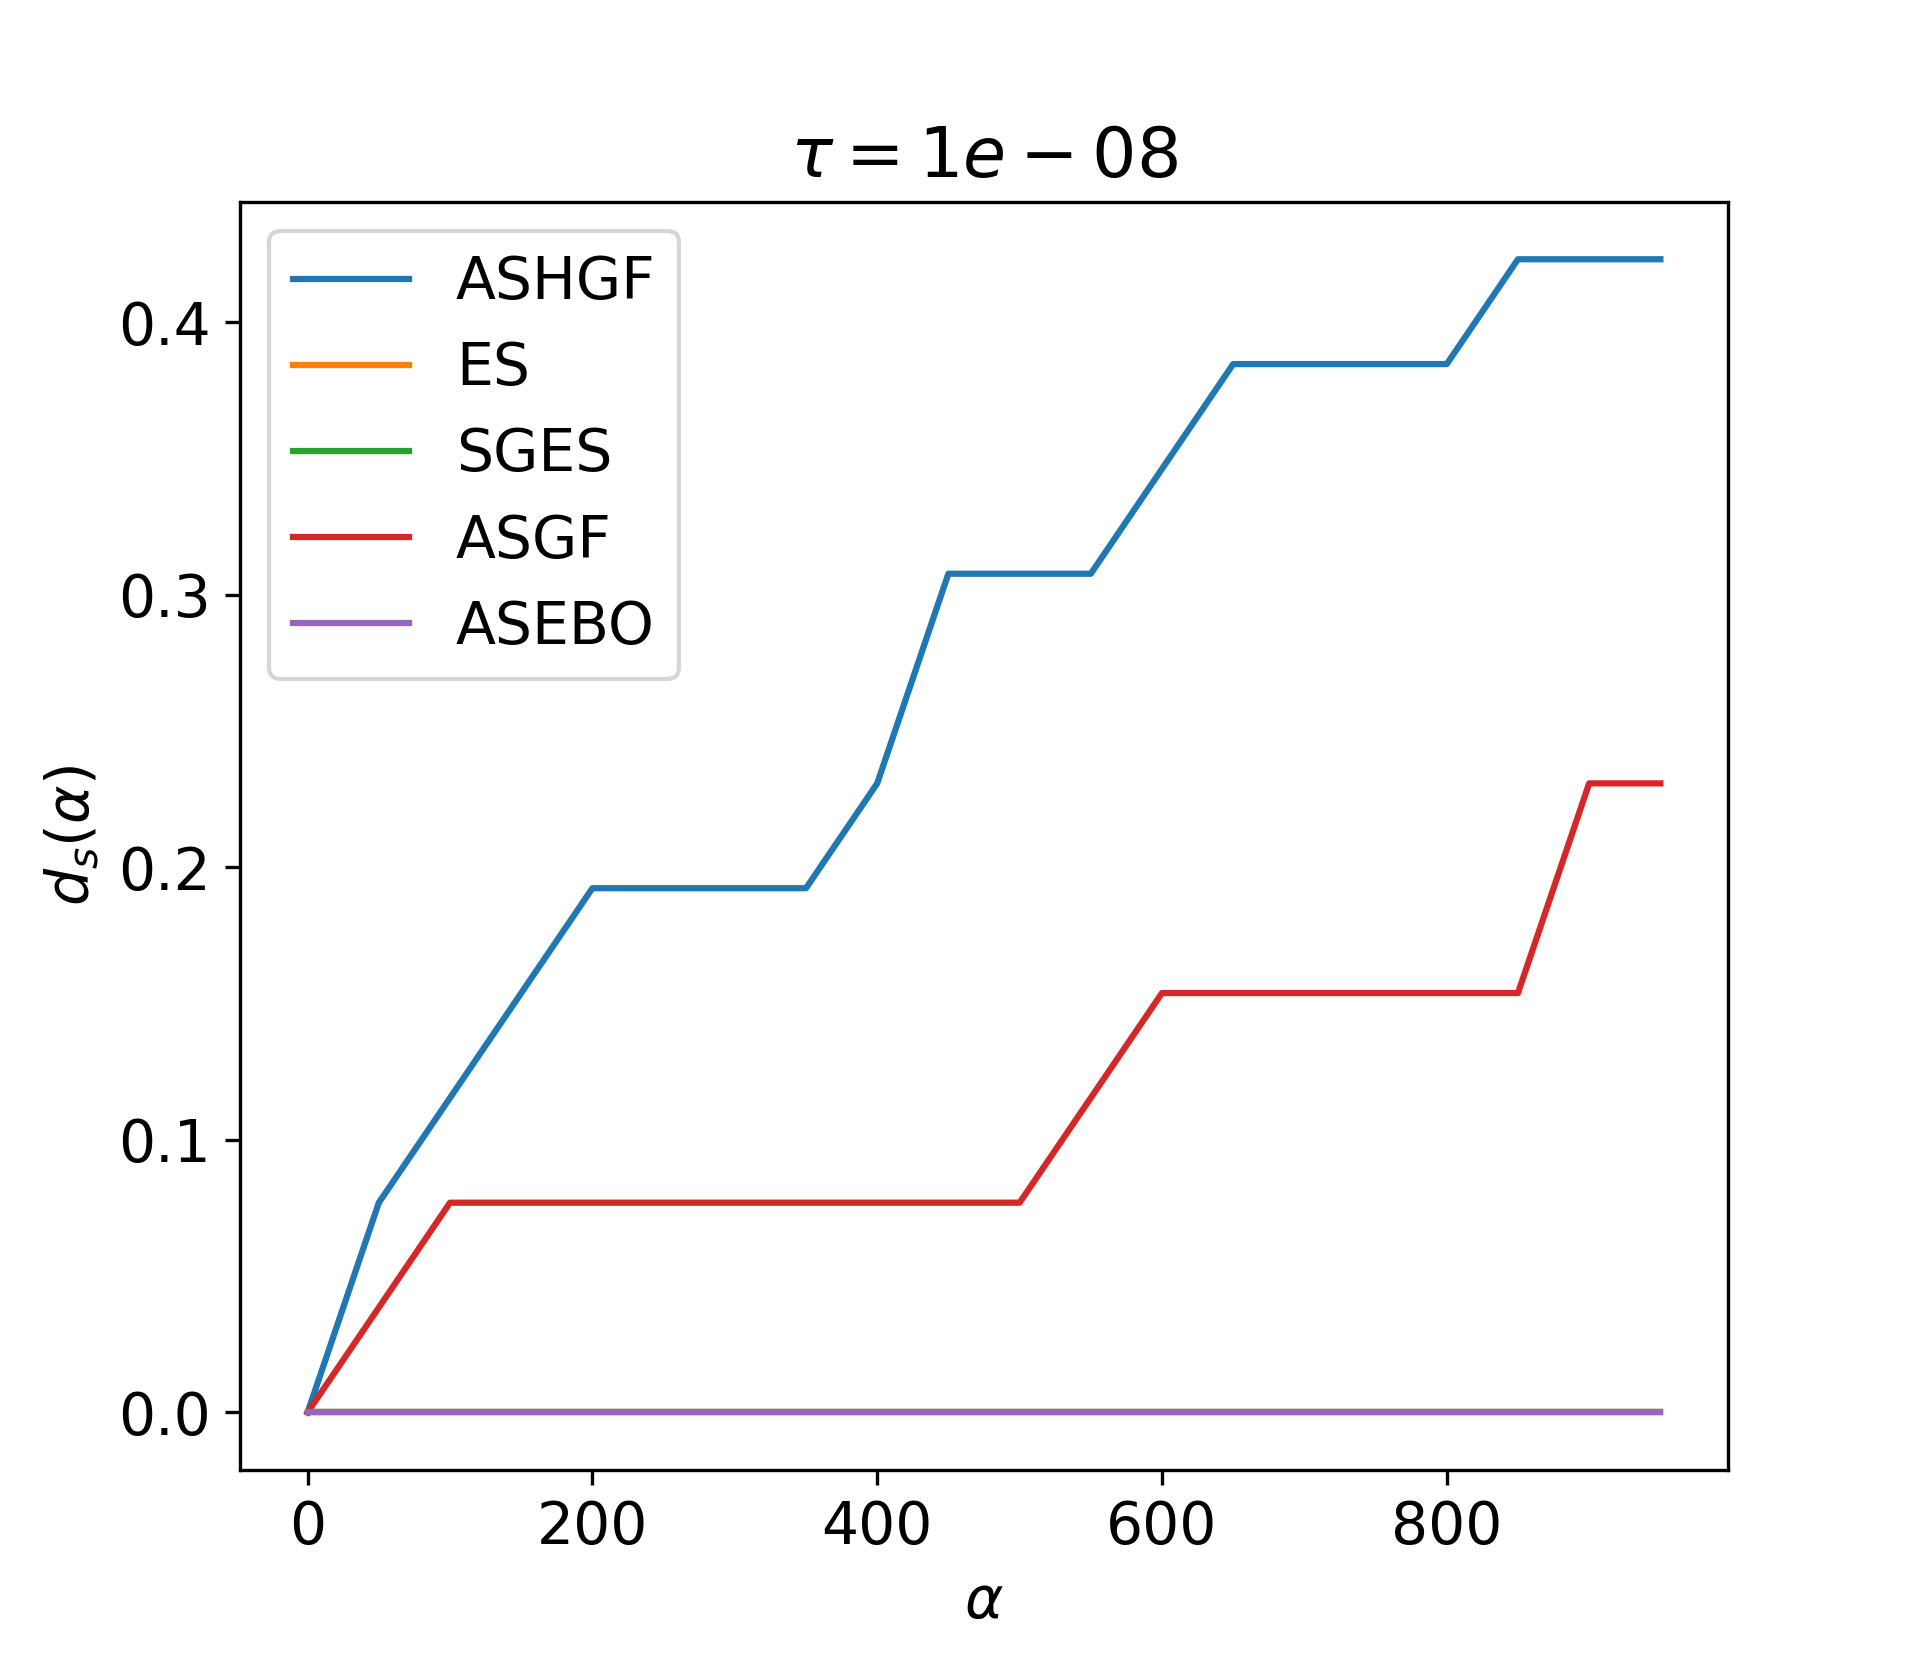
\includegraphics[width=1\textwidth]{figures/data_profiles/100/data_profile_100_10000000_1e-08.png}
\end{subfigure}%
\begin{subfigure}{0.3\textwidth}
  \centering 
  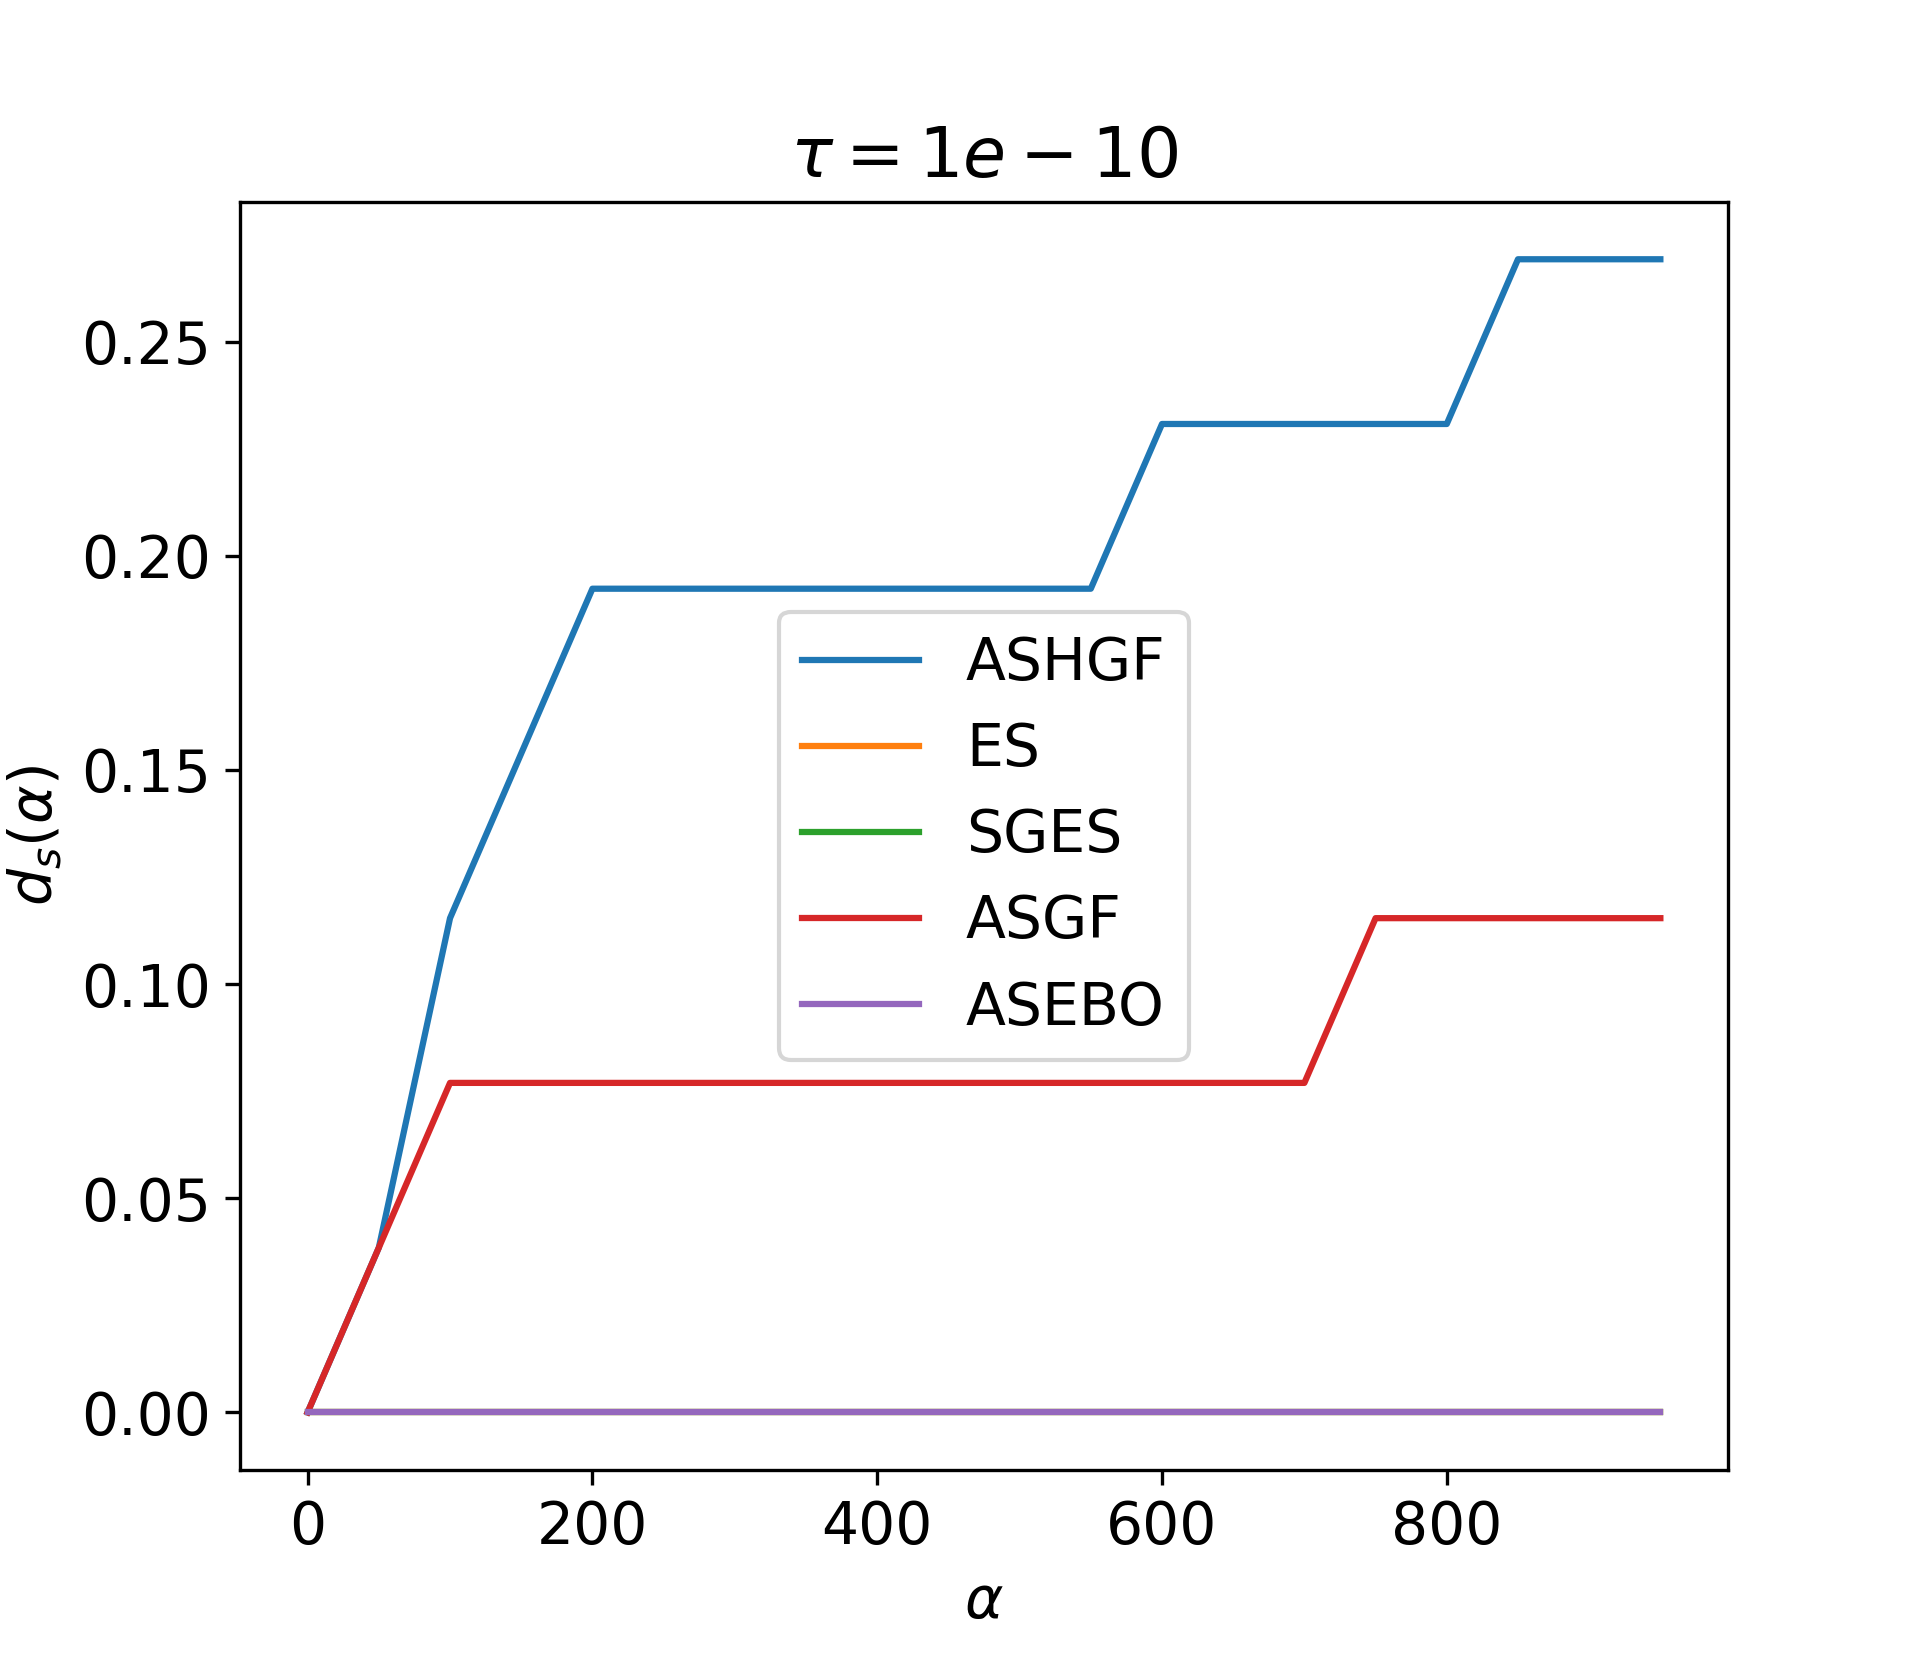
\includegraphics[width=1\textwidth]{figures/data_profiles/100/data_profile_100_10000000_1e-10.png}
\end{subfigure}
\caption{Data profiles with $\mu_L = 10^{7}$}
\label{DataProfiles100Mu10000000}
\end{figure}

\begin{figure}[H]
	\centering
	\begin{subfigure}{0.3\textwidth}
		\centering 
		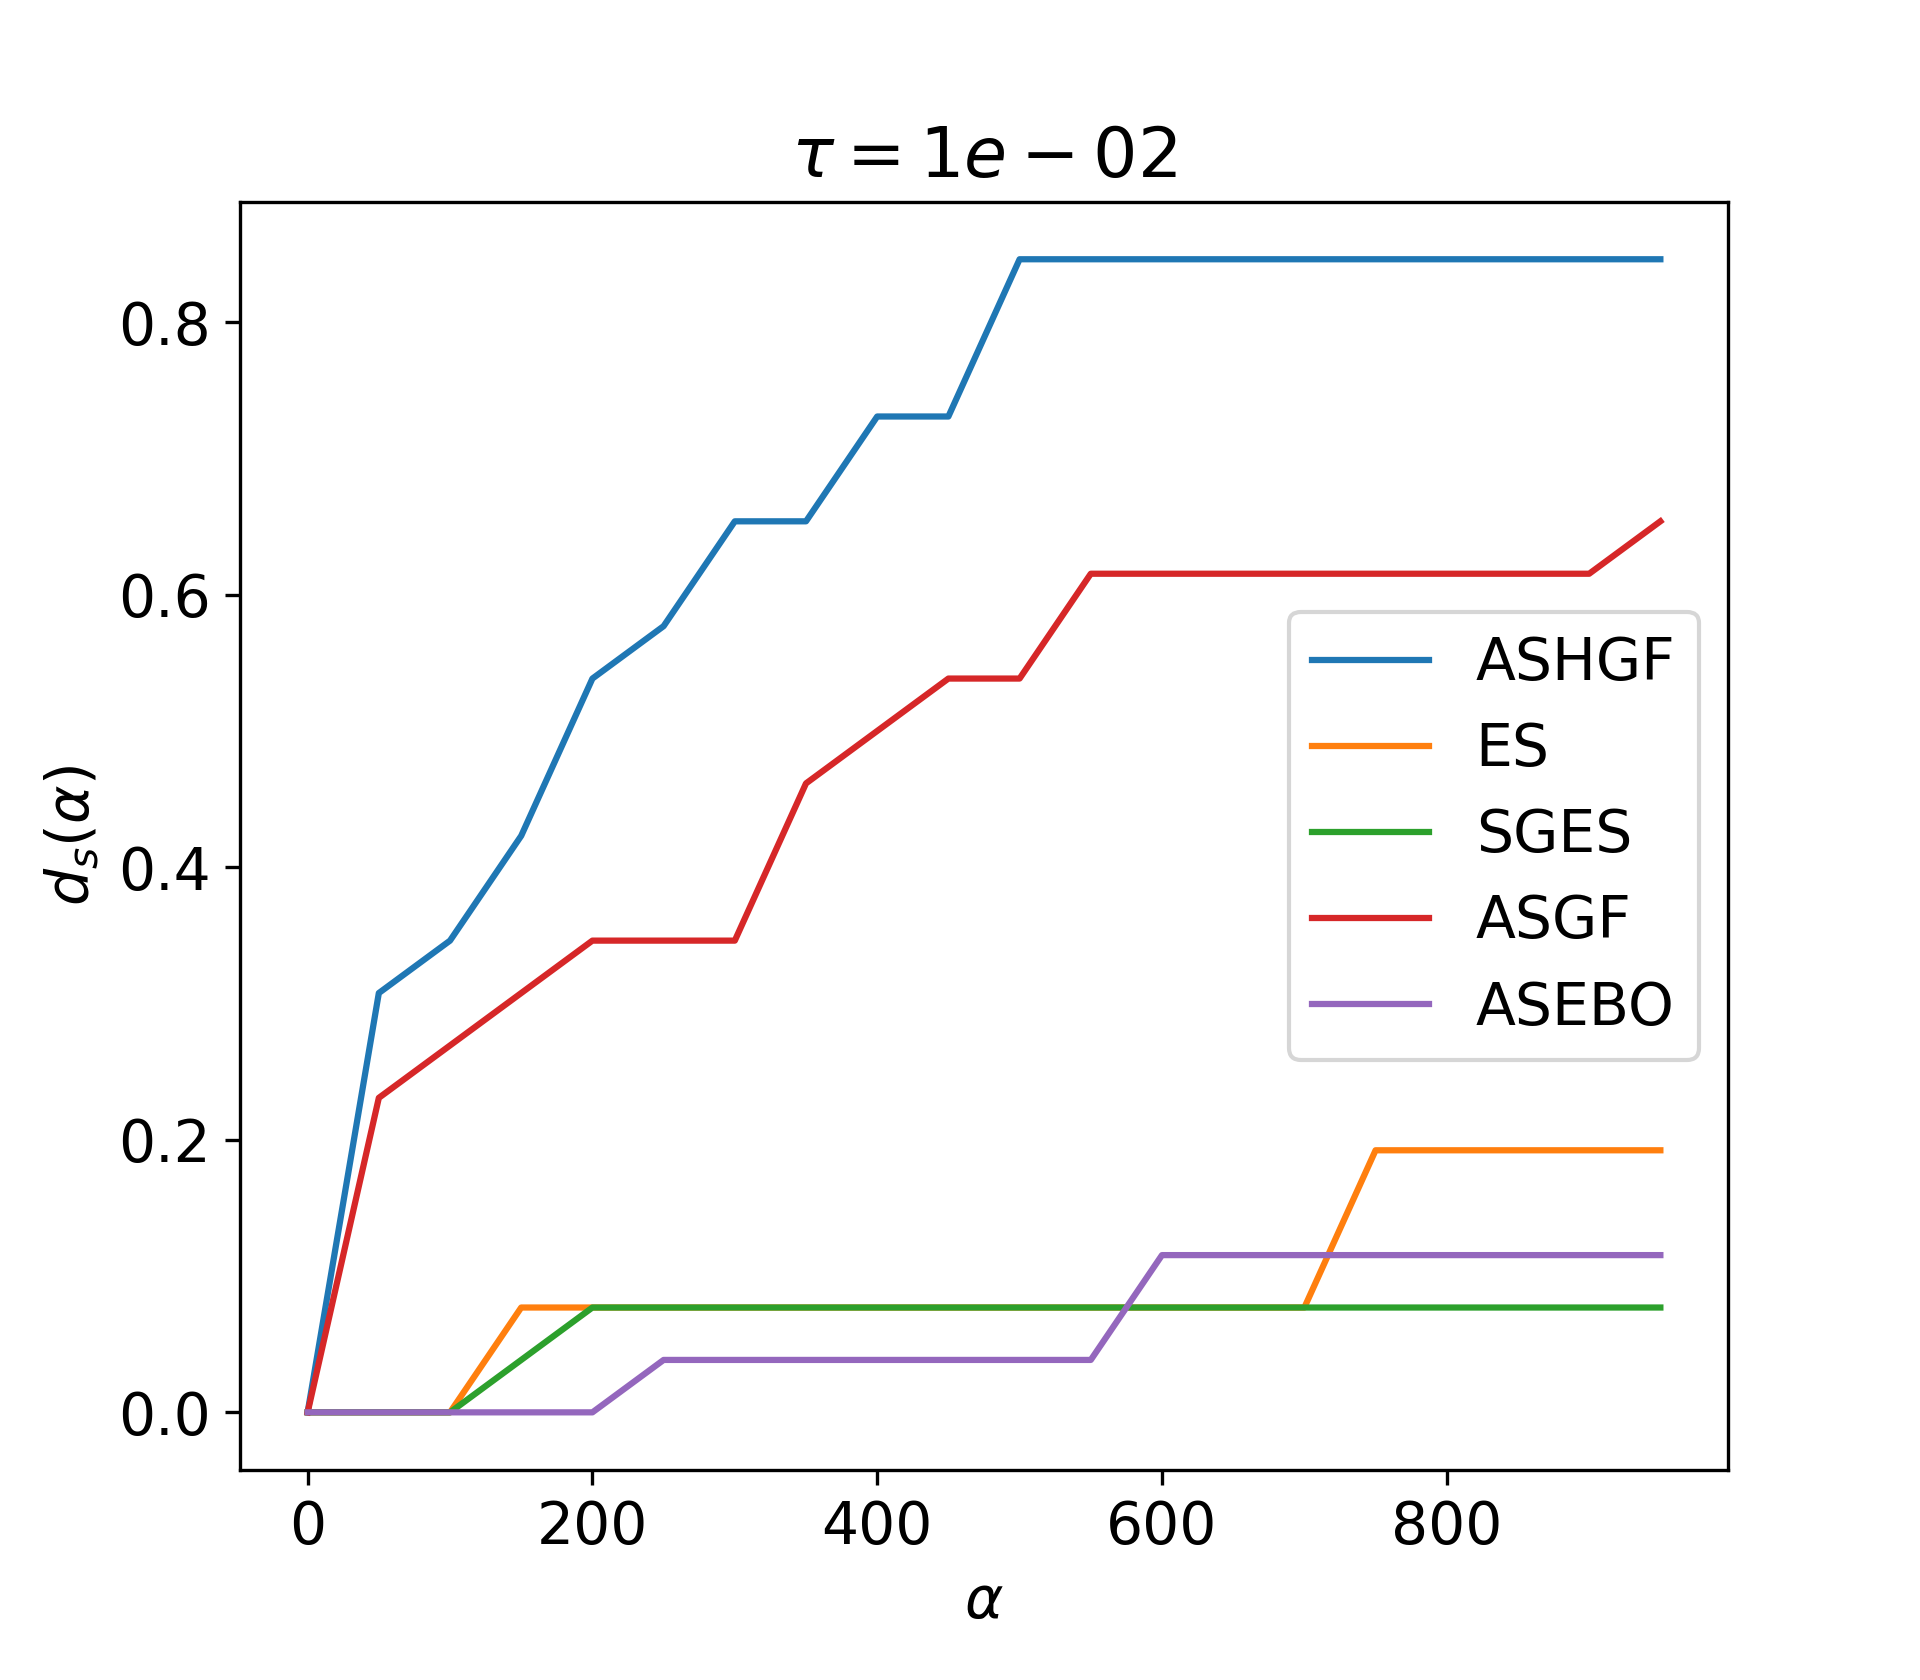
\includegraphics[width=1\textwidth]{figures/data_profiles/100/data_profile_100_100000000_1e-02.png}
	\end{subfigure}%
	\begin{subfigure}{0.3\textwidth}
		\centering 
		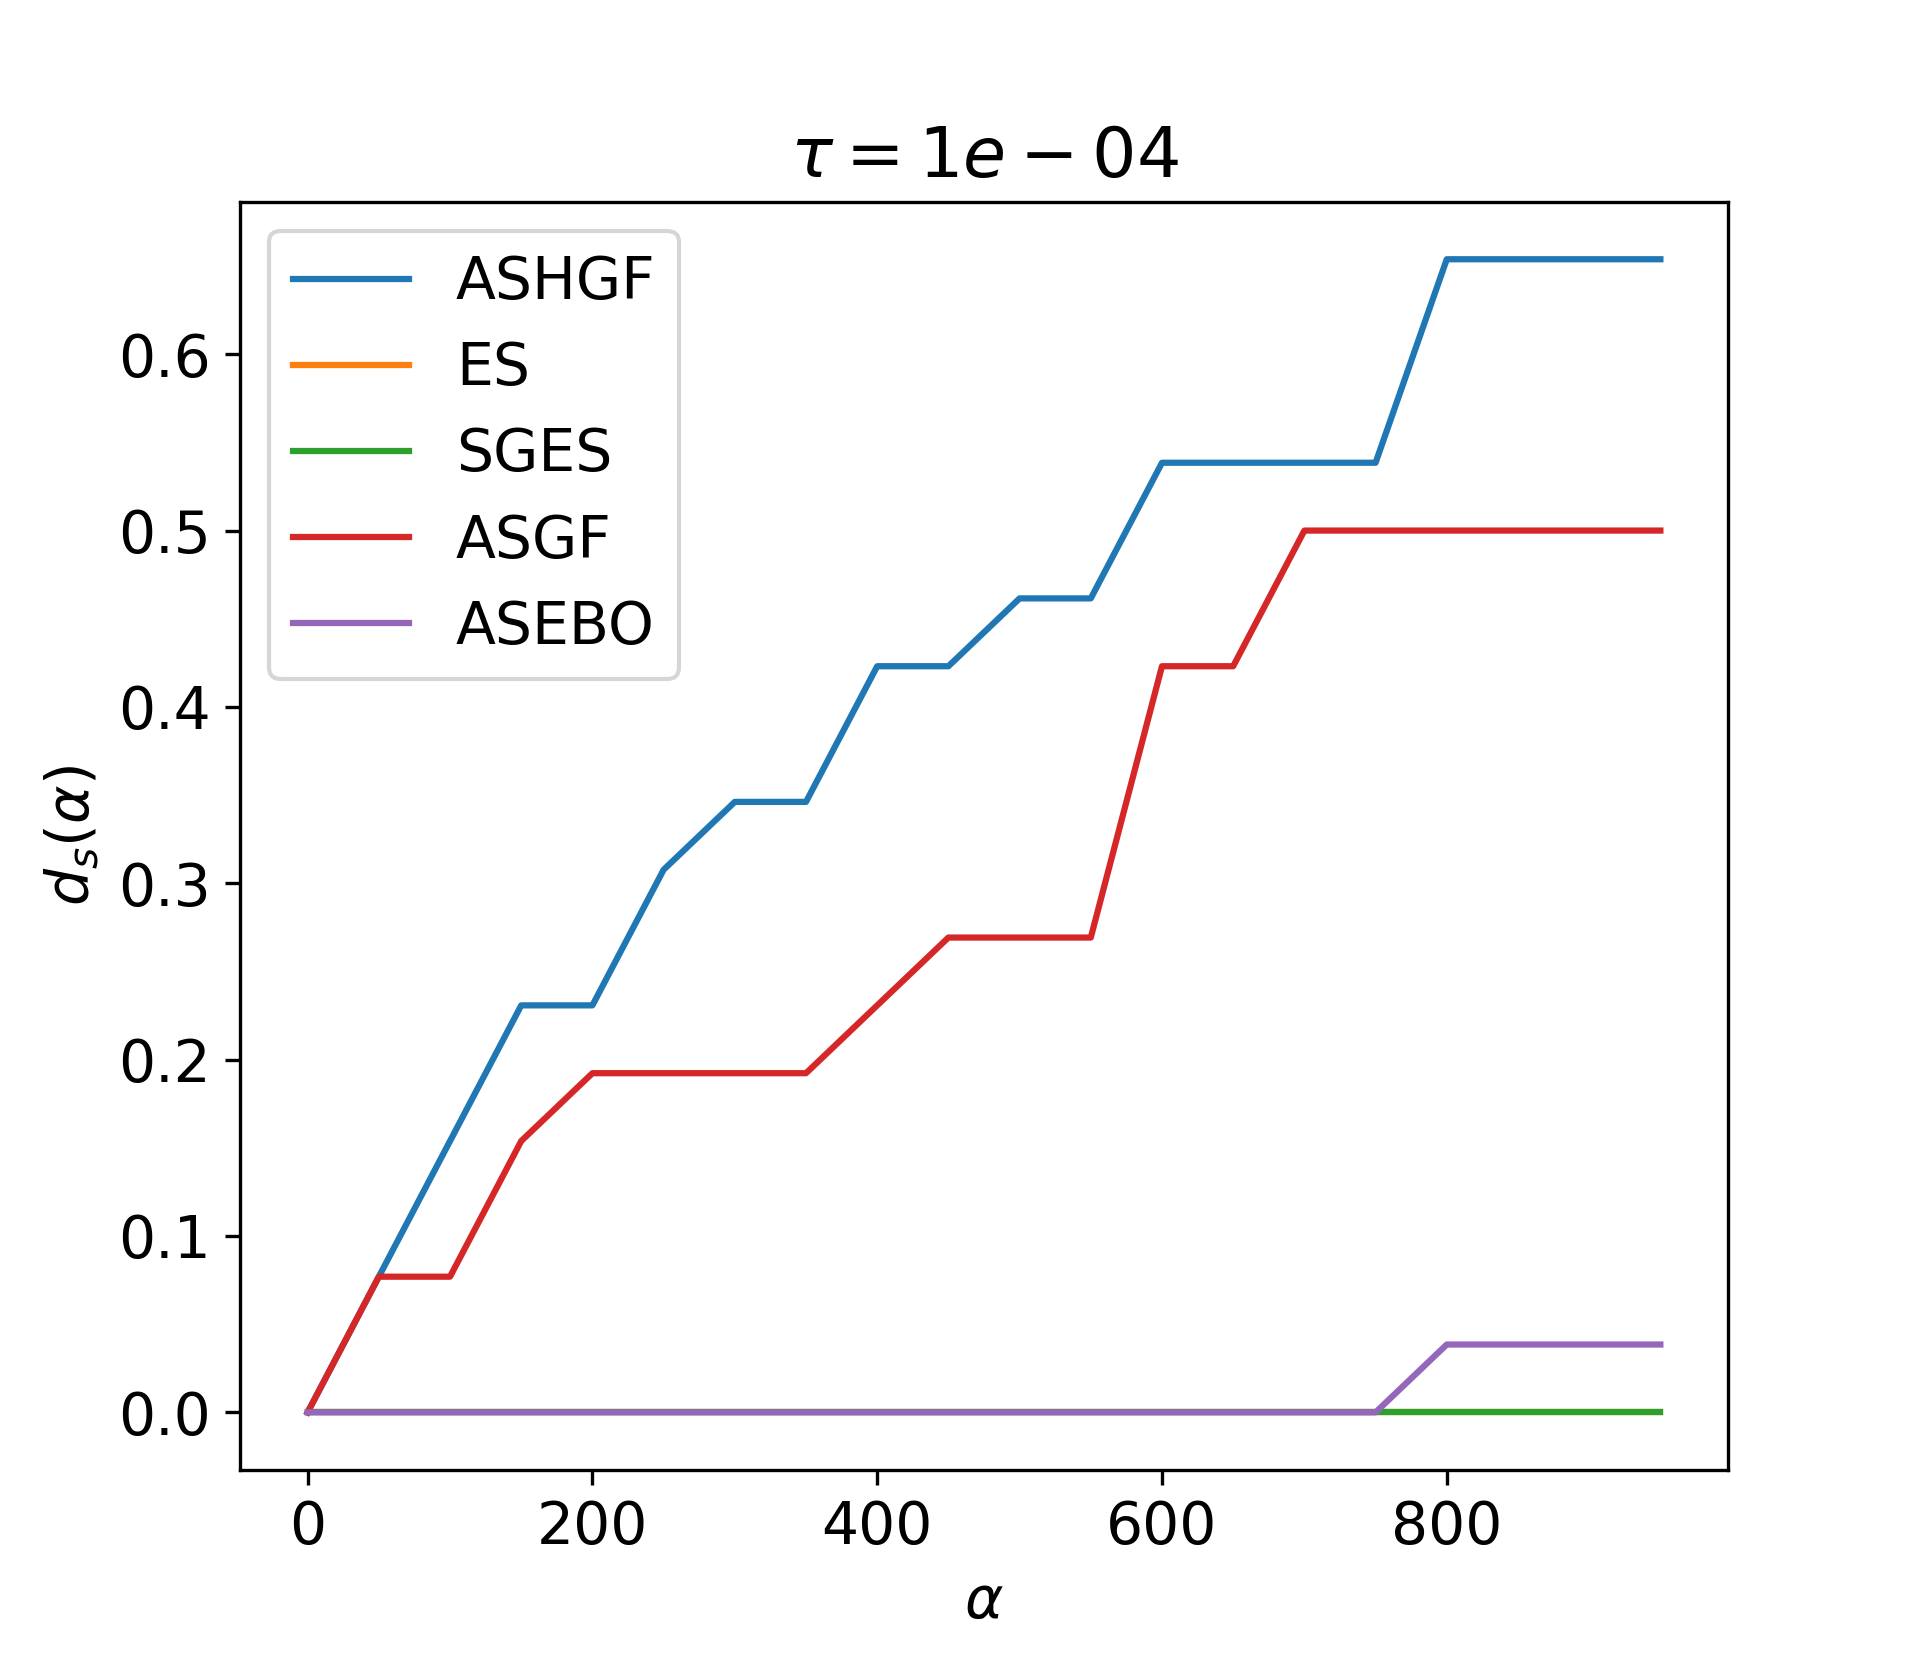
\includegraphics[width=1\textwidth]{figures/data_profiles/100/data_profile_100_100000000_1e-04.png}
	\end{subfigure}
	\begin{subfigure}{0.3\textwidth}
		\centering 
		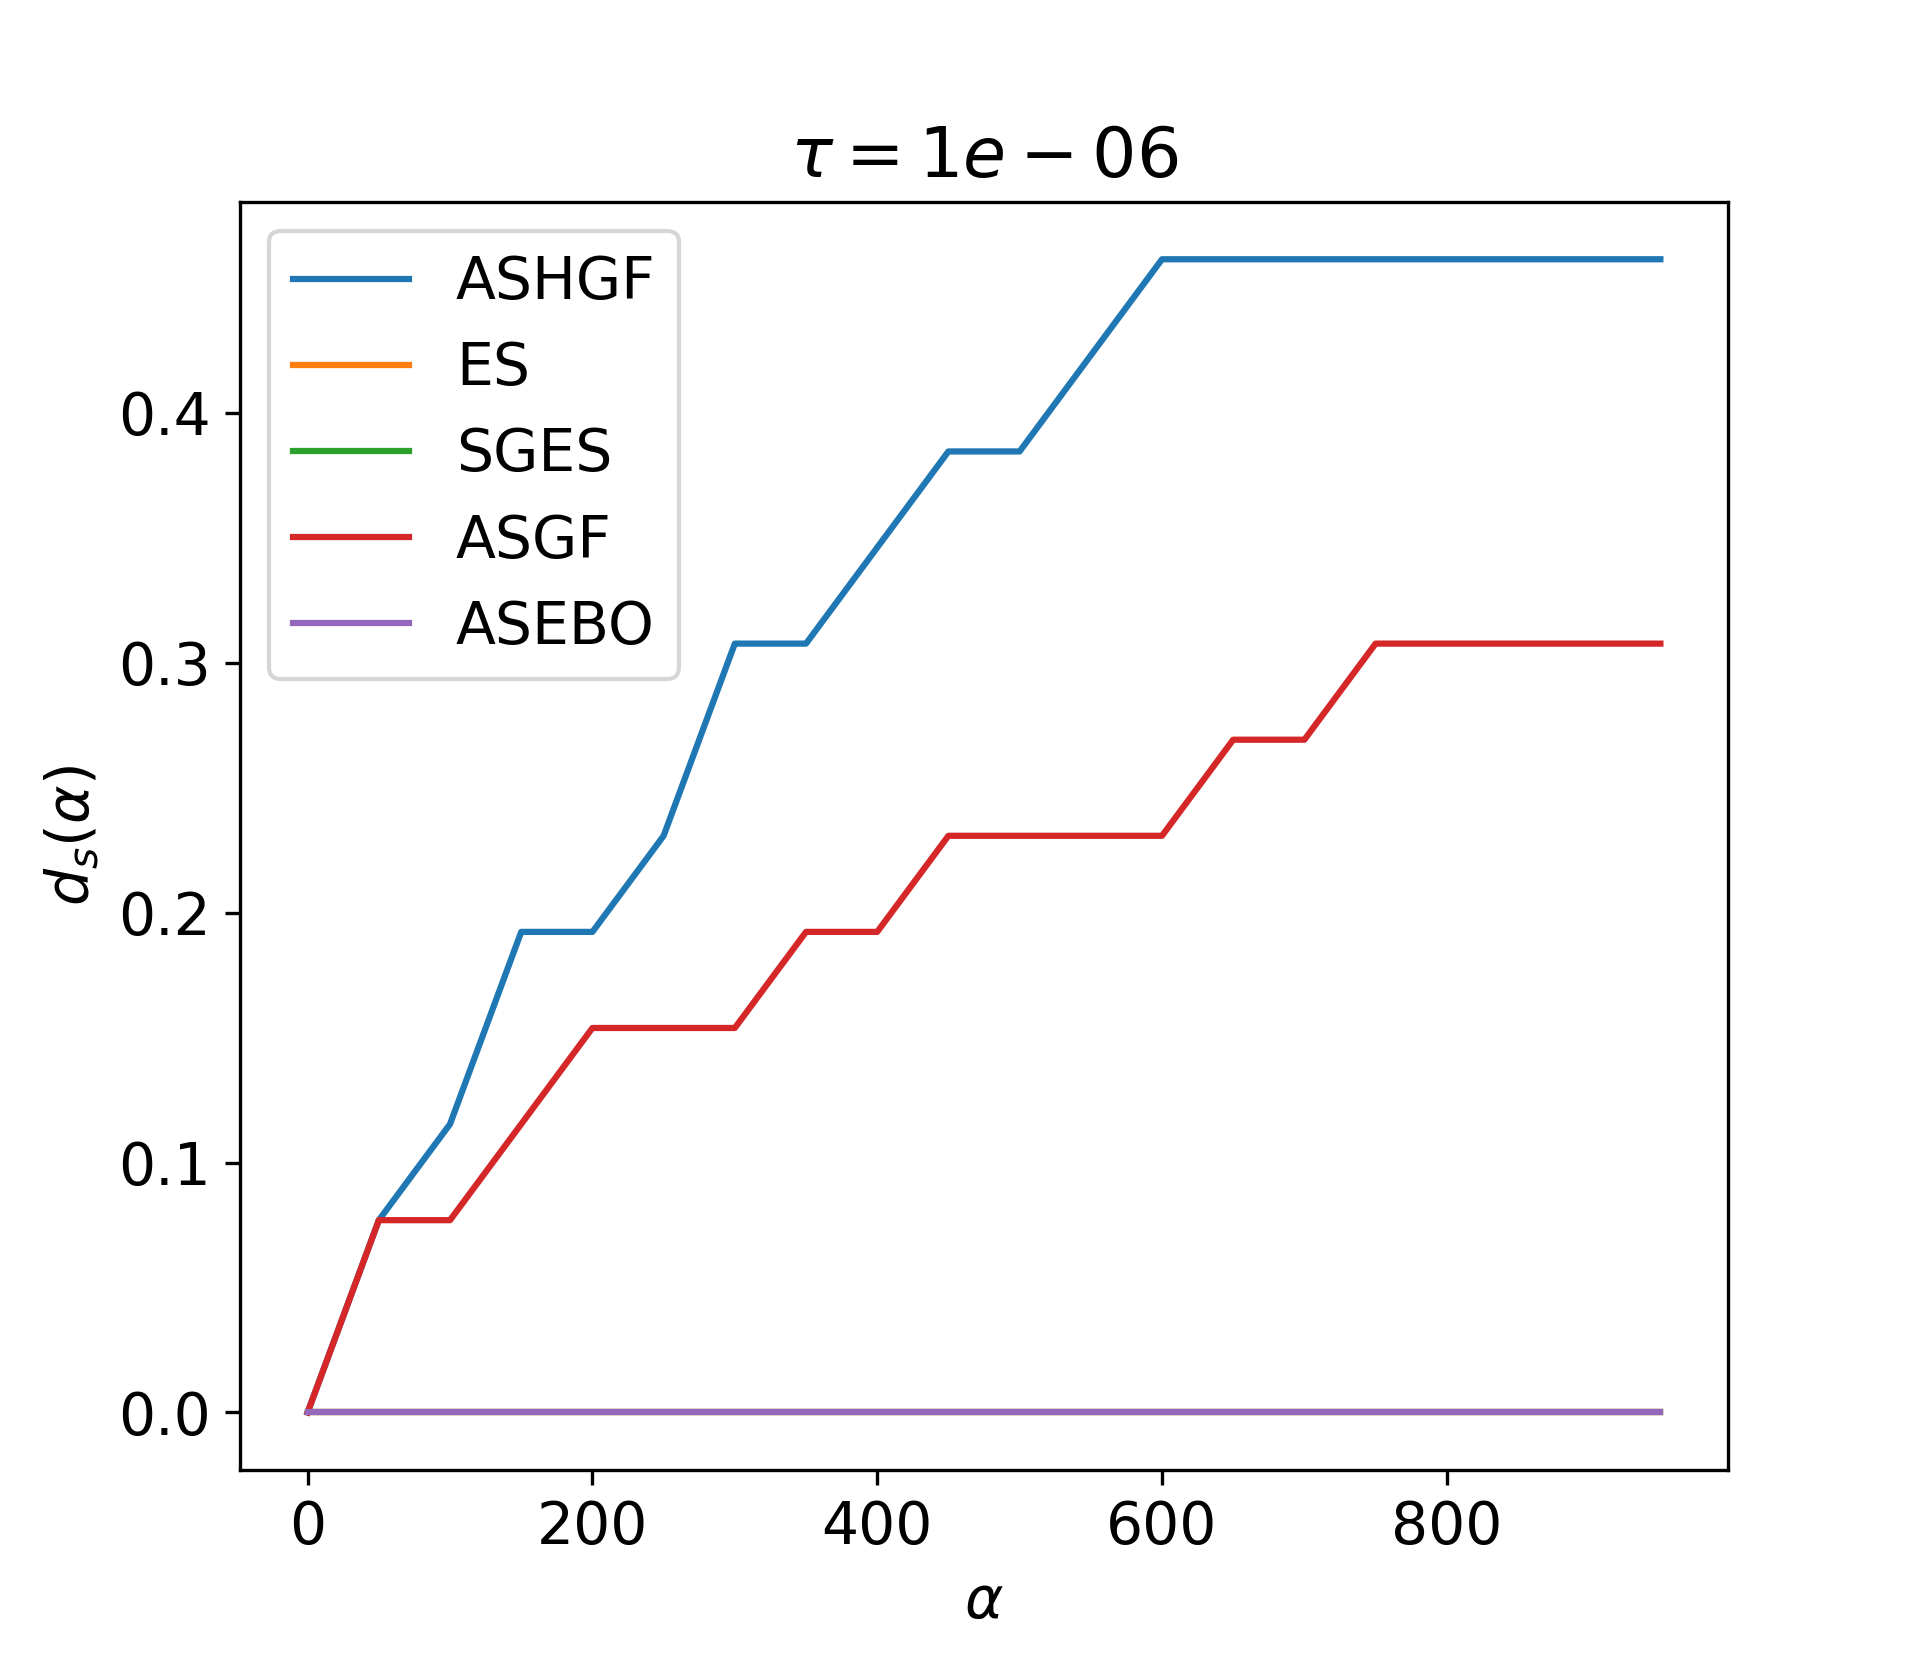
\includegraphics[width=1\textwidth]{figures/data_profiles/100/data_profile_100_100000000_1e-06.png}
	\end{subfigure}
	\centering
	\begin{subfigure}{0.3\textwidth}
		\centering 
		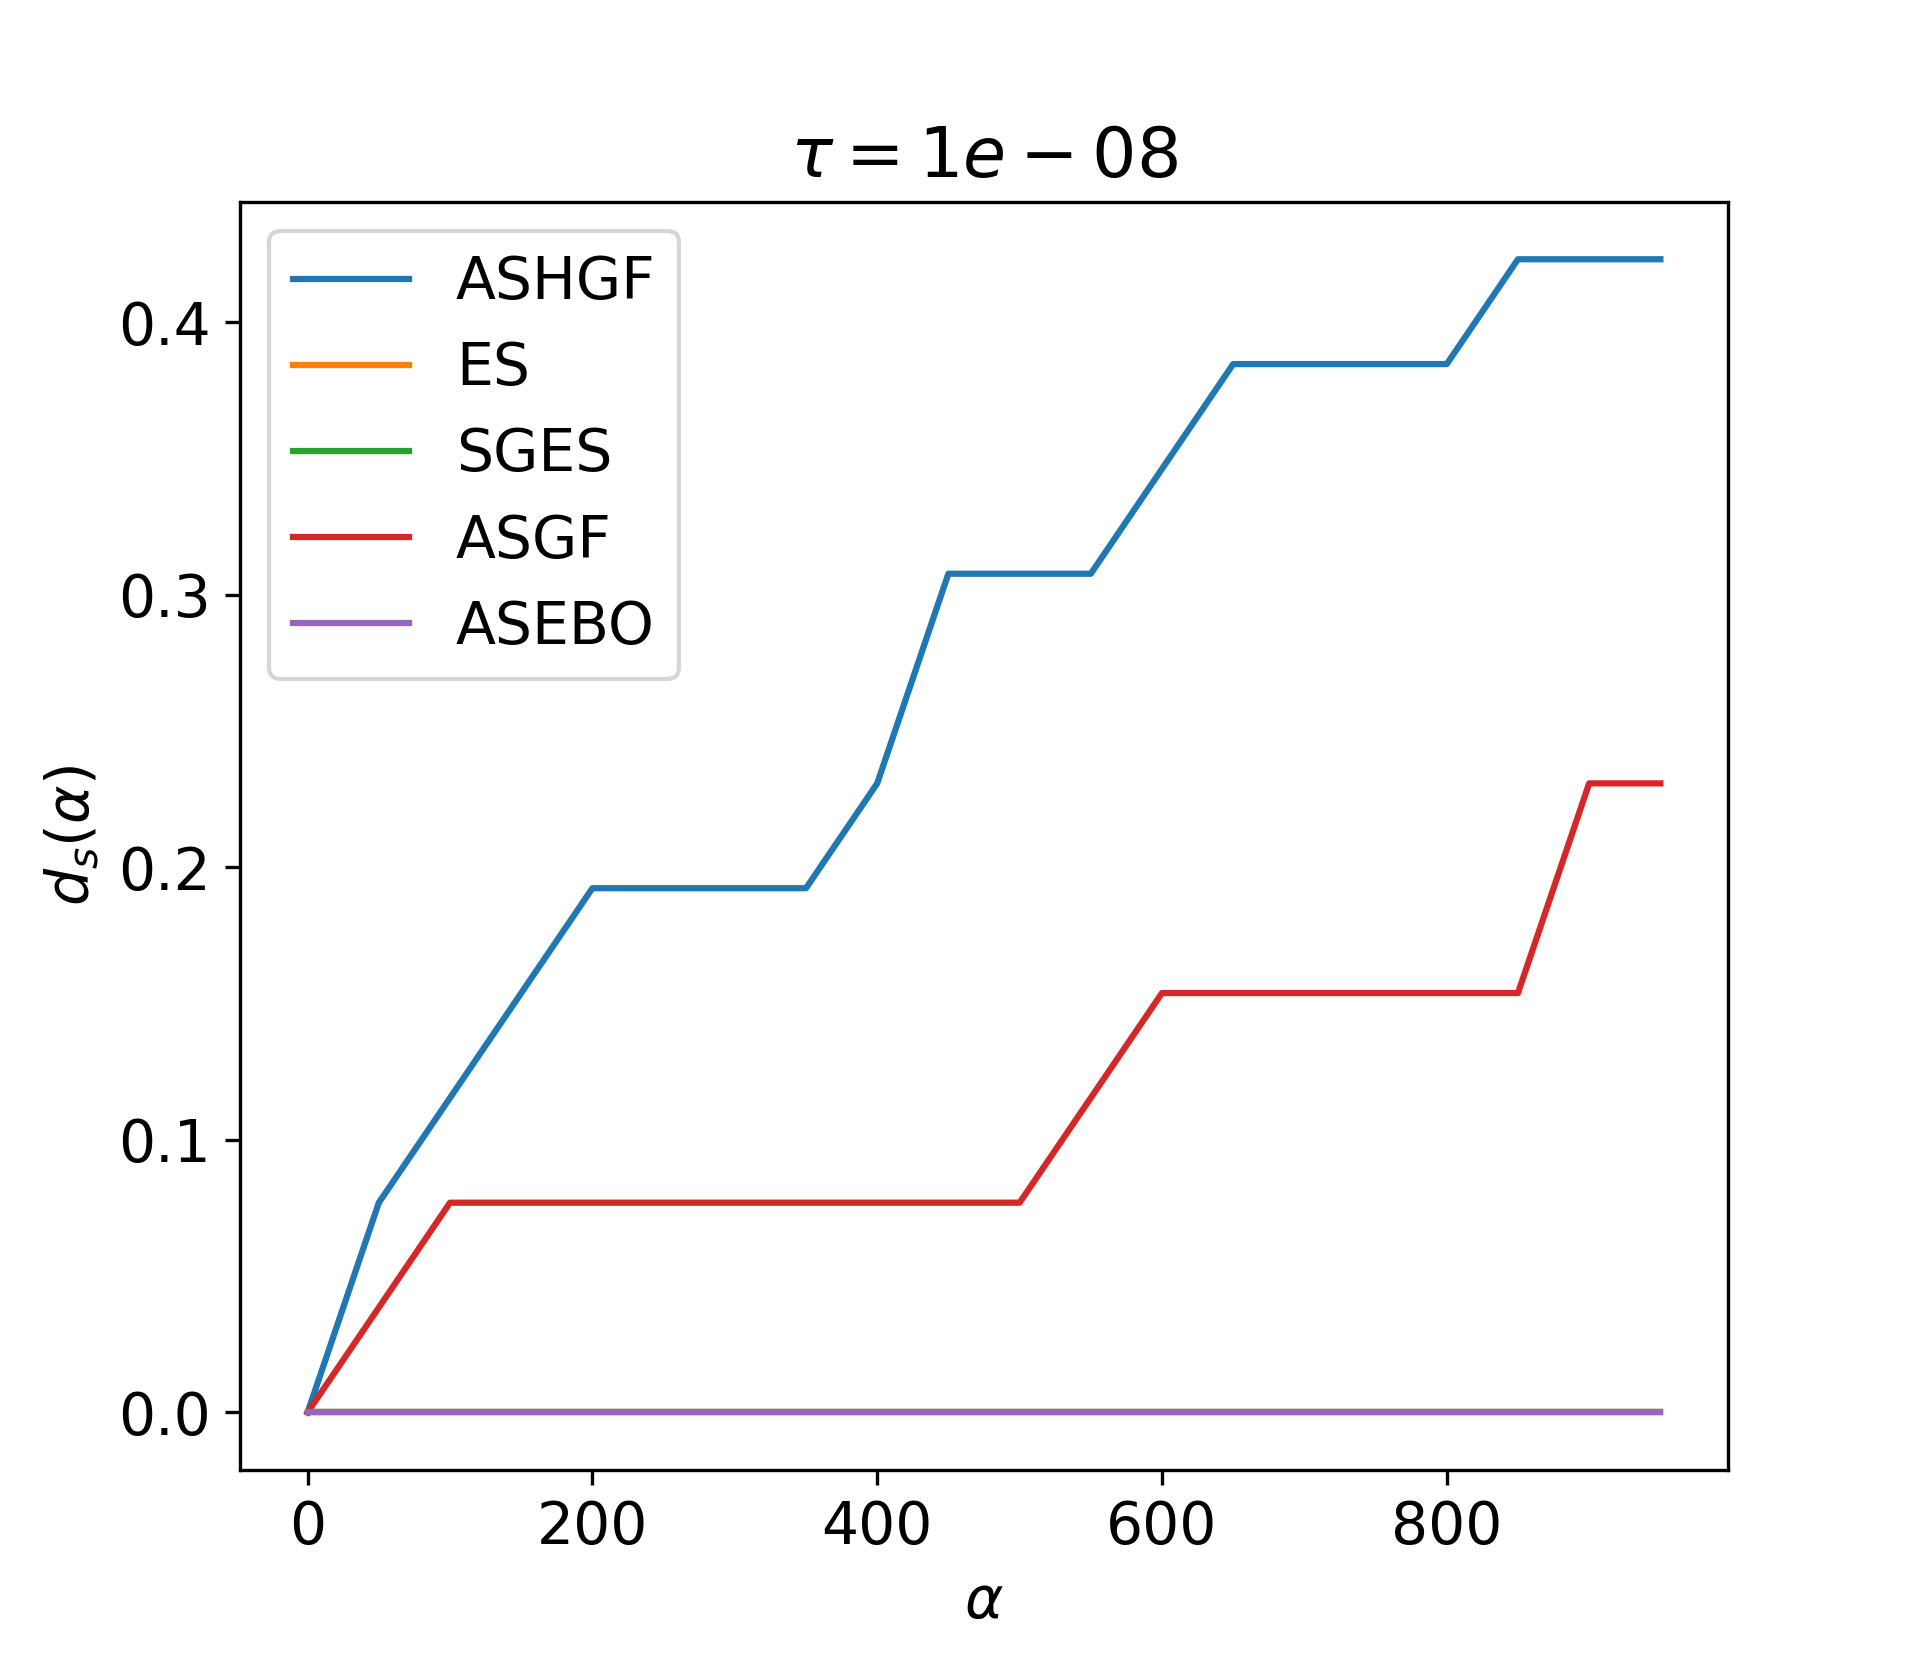
\includegraphics[width=1\textwidth]{figures/data_profiles/100/data_profile_100_100000000_1e-08.png}
	\end{subfigure}%
	\begin{subfigure}{0.3\textwidth}
		\centering 
		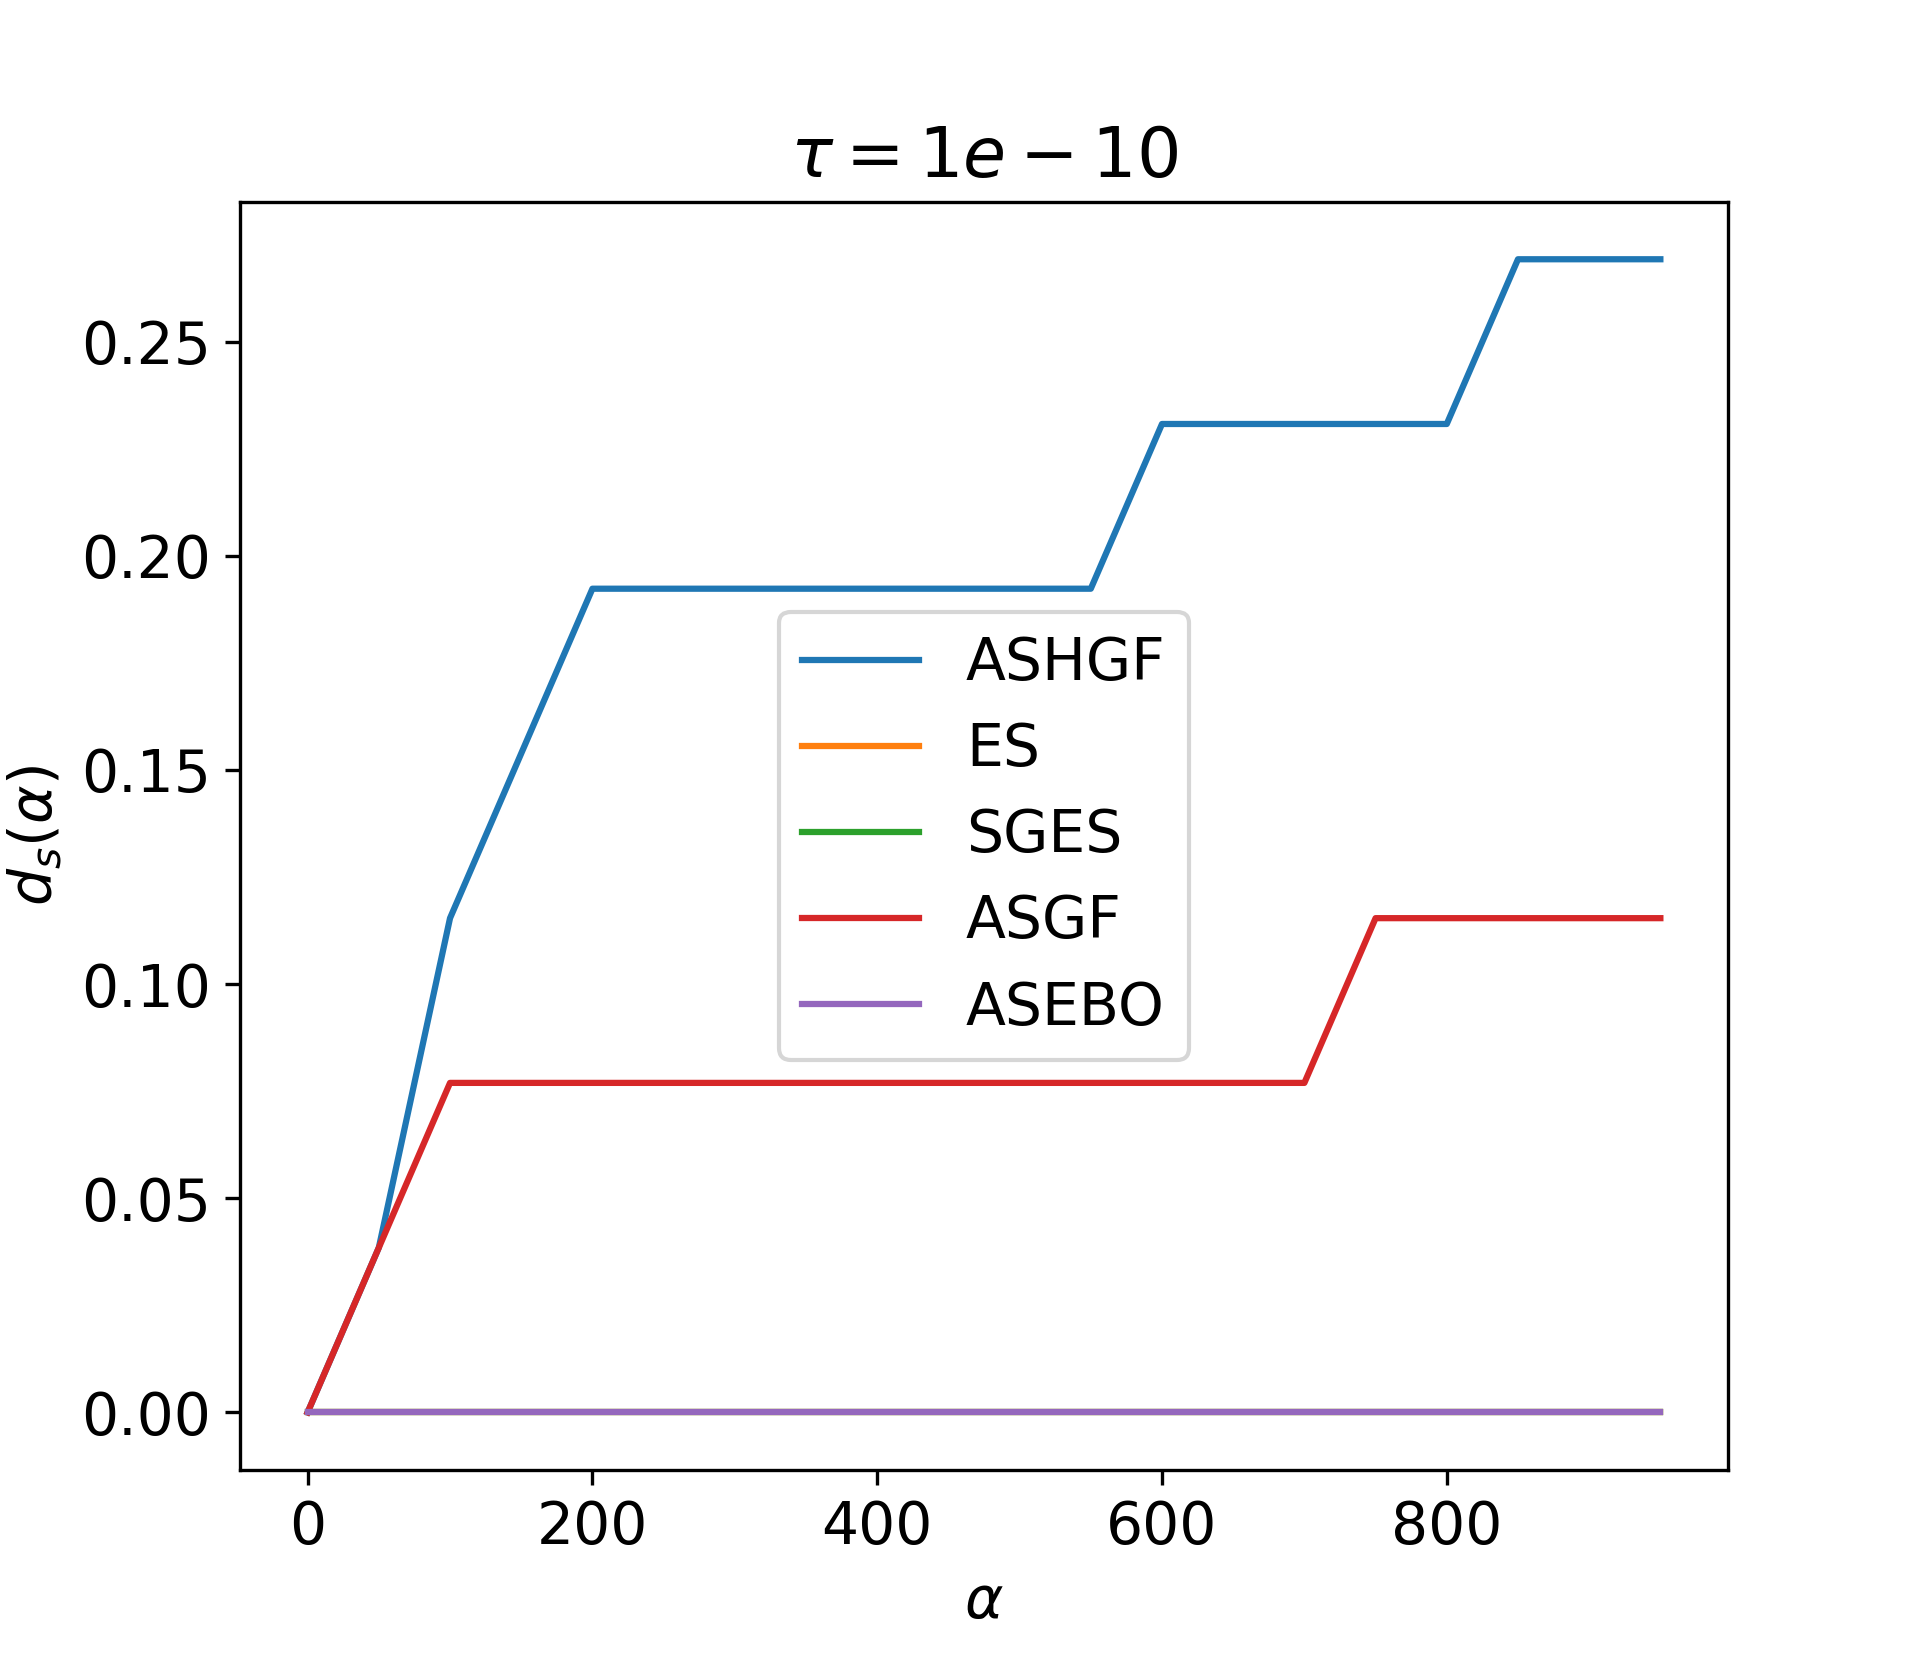
\includegraphics[width=1\textwidth]{figures/data_profiles/100/data_profile_100_100000000_1e-10.png}
	\end{subfigure}
	\caption{Data profiles with $\mu_L = 10^{8}$}
	\label{DataProfiles100Mu100000000}
\end{figure}

\subsubsection{Dimension 1000}

\begin{figure}[H]
\centering
\begin{subfigure}{0.3\textwidth}
  \centering 
  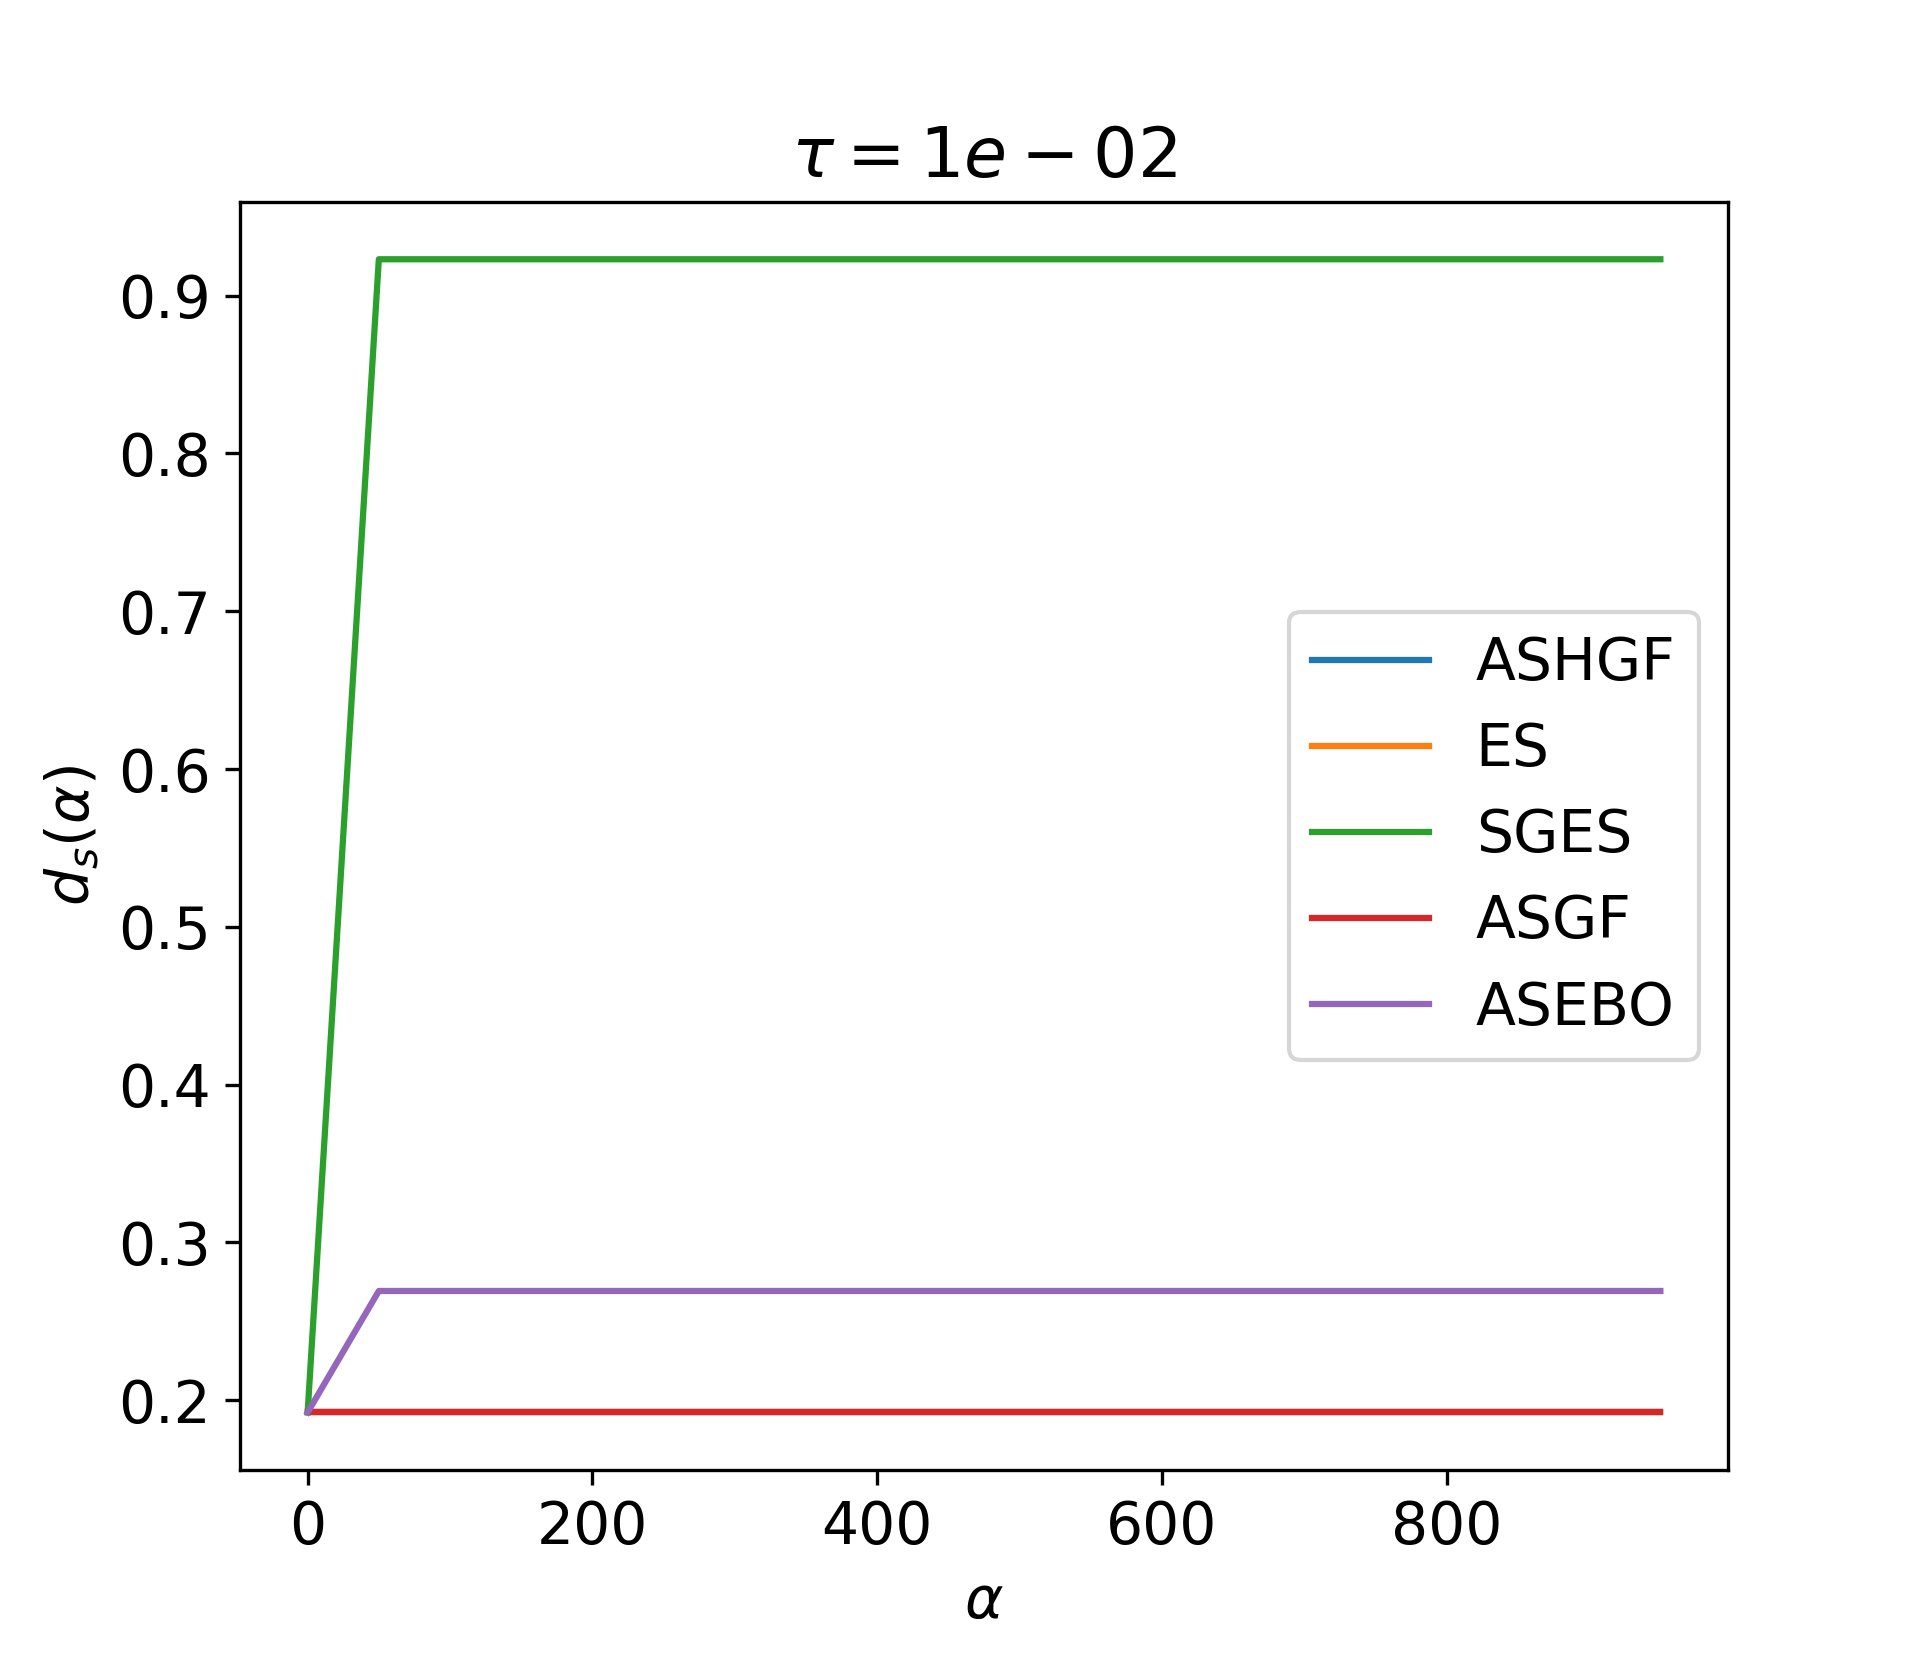
\includegraphics[width=1\textwidth]{figures/data_profiles/1000/data_profile_1000_10000_1e-02.png}
\end{subfigure}%
\begin{subfigure}{0.3\textwidth}
  \centering 
  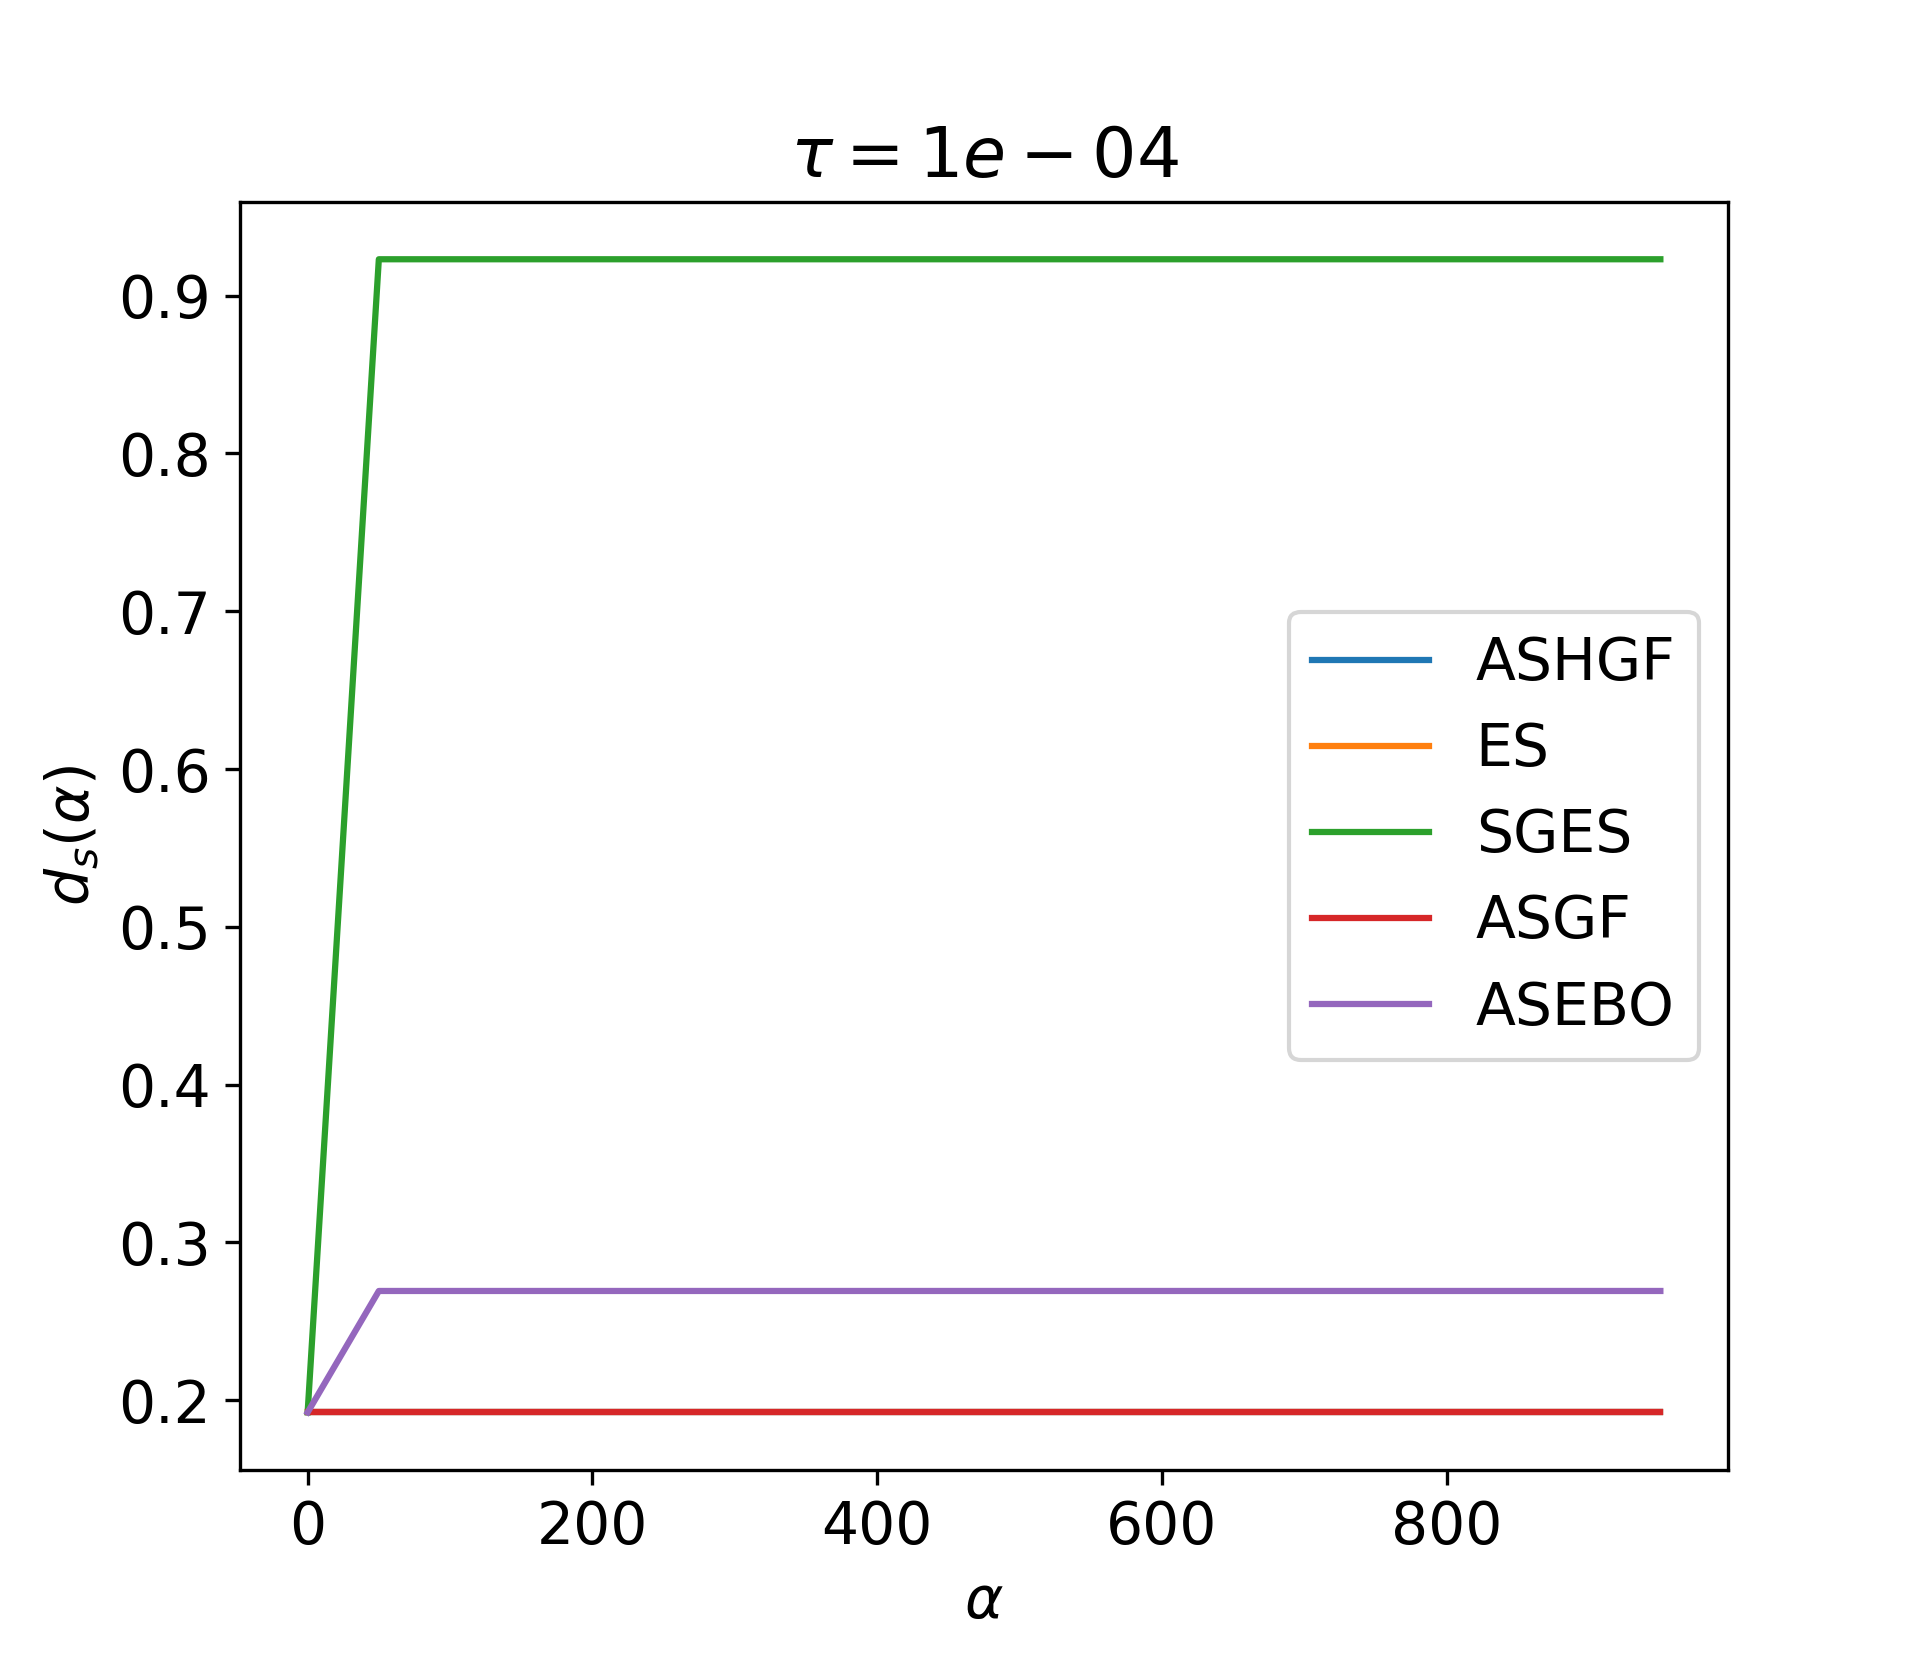
\includegraphics[width=1\textwidth]{figures/data_profiles/1000/data_profile_1000_10000_1e-04.png}
\end{subfigure}
\begin{subfigure}{0.3\textwidth}
  \centering 
  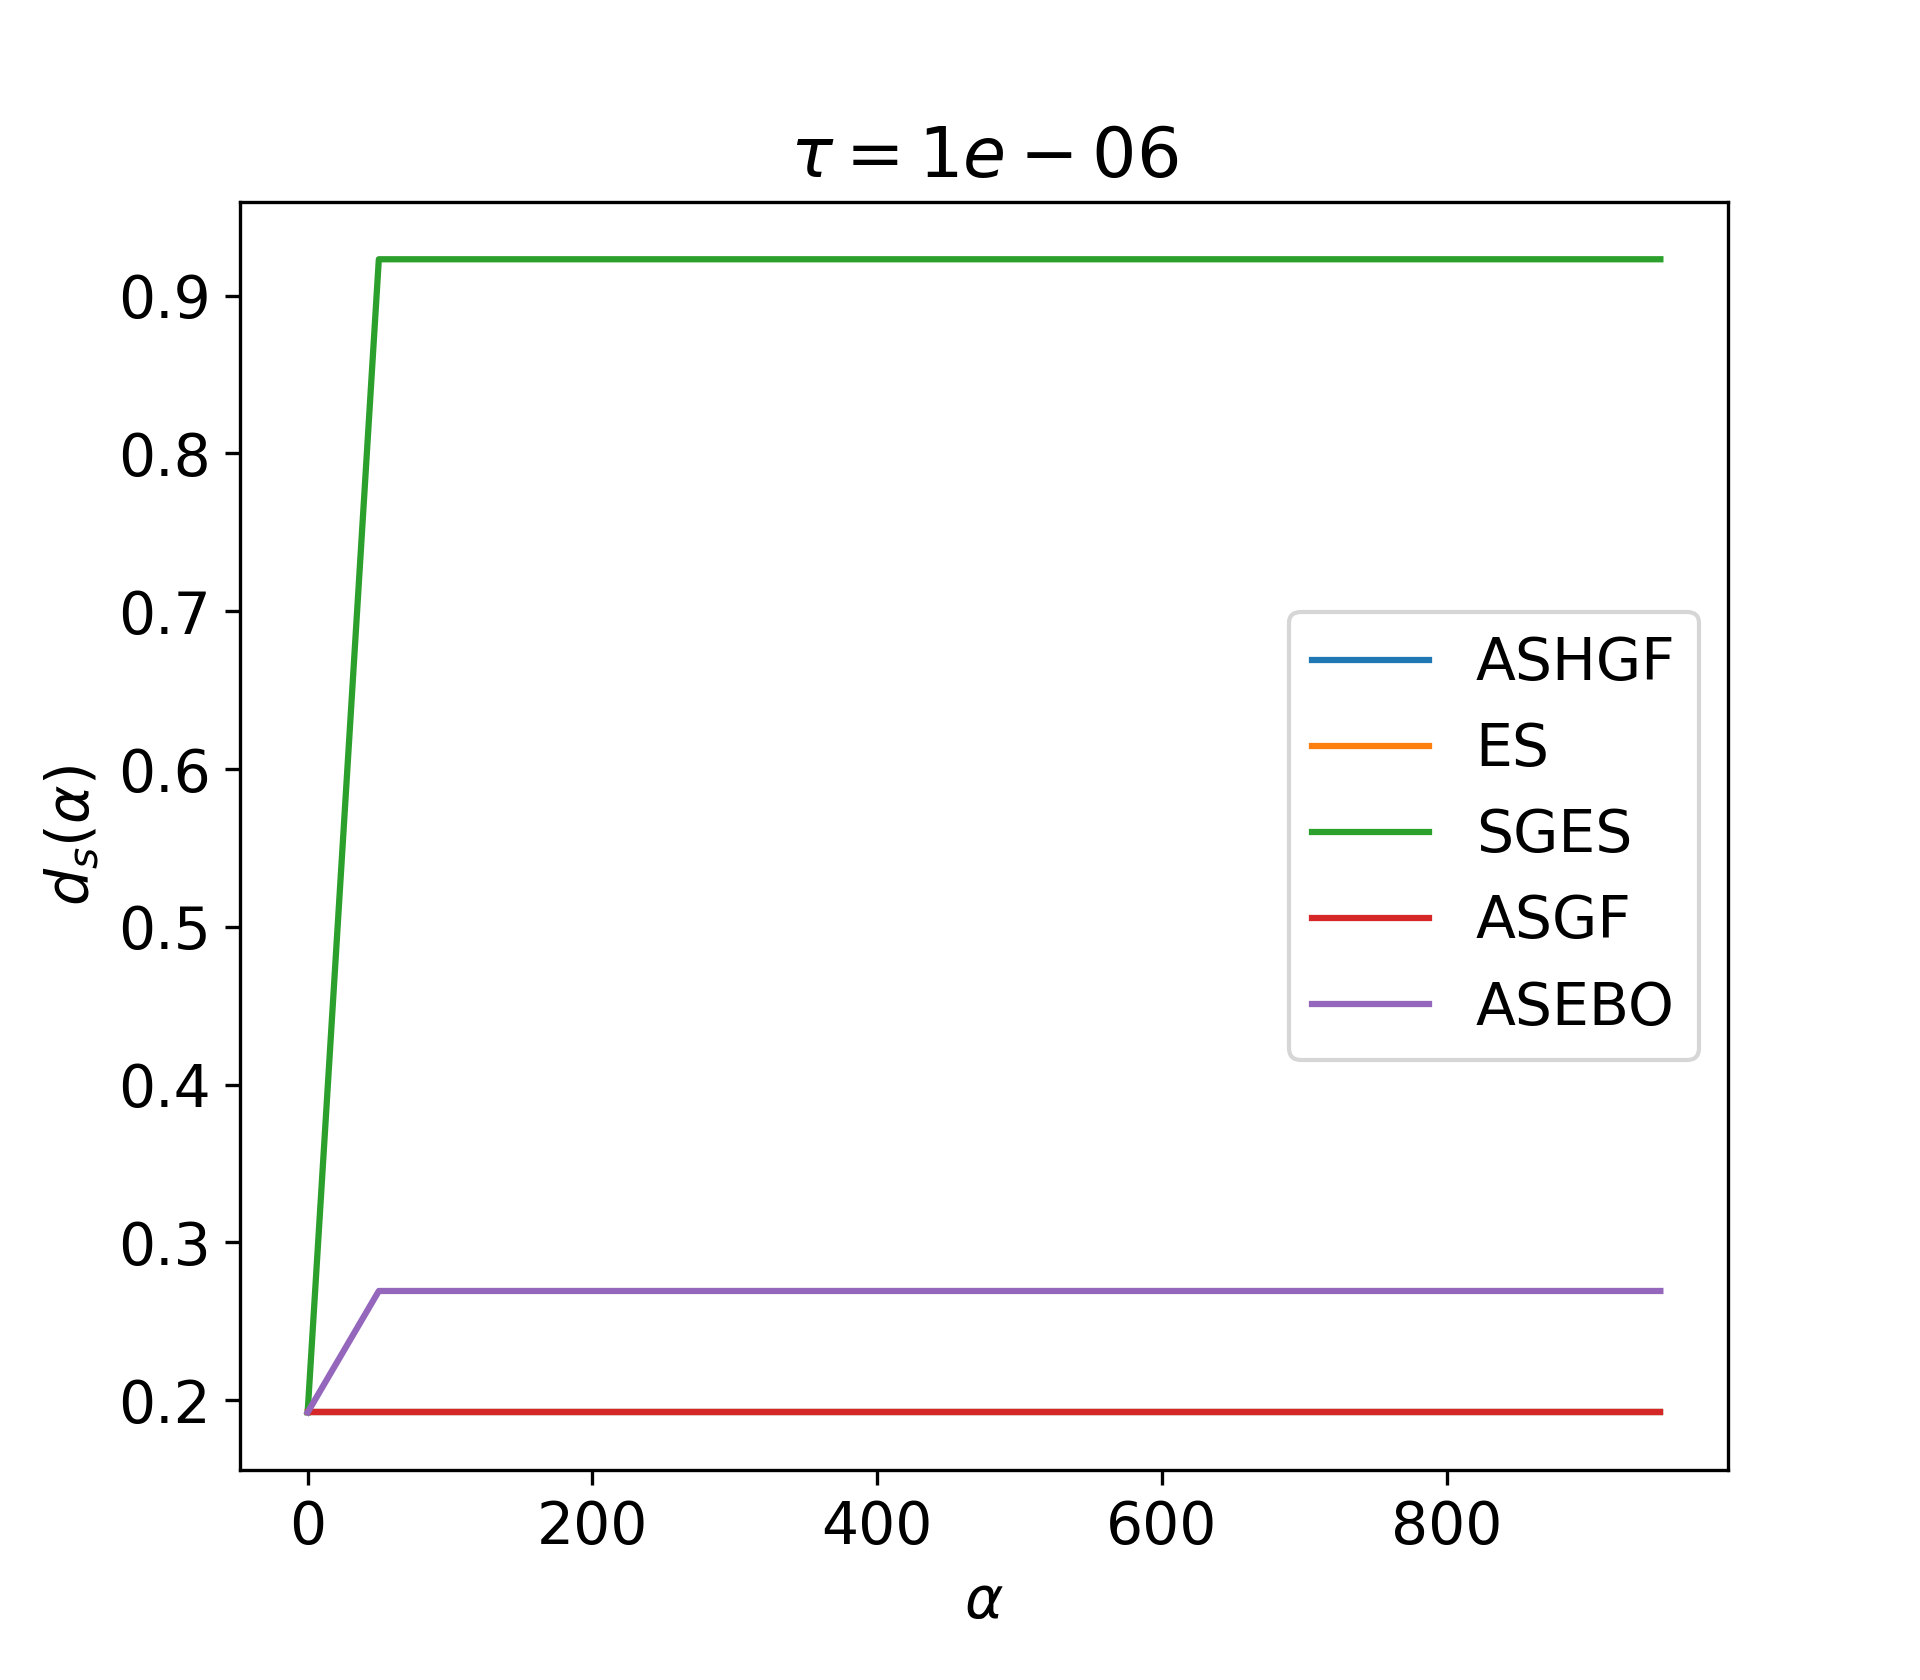
\includegraphics[width=1\textwidth]{figures/data_profiles/1000/data_profile_1000_10000_1e-06.png}
\end{subfigure}
\centering
\begin{subfigure}{0.3\textwidth}
  \centering 
  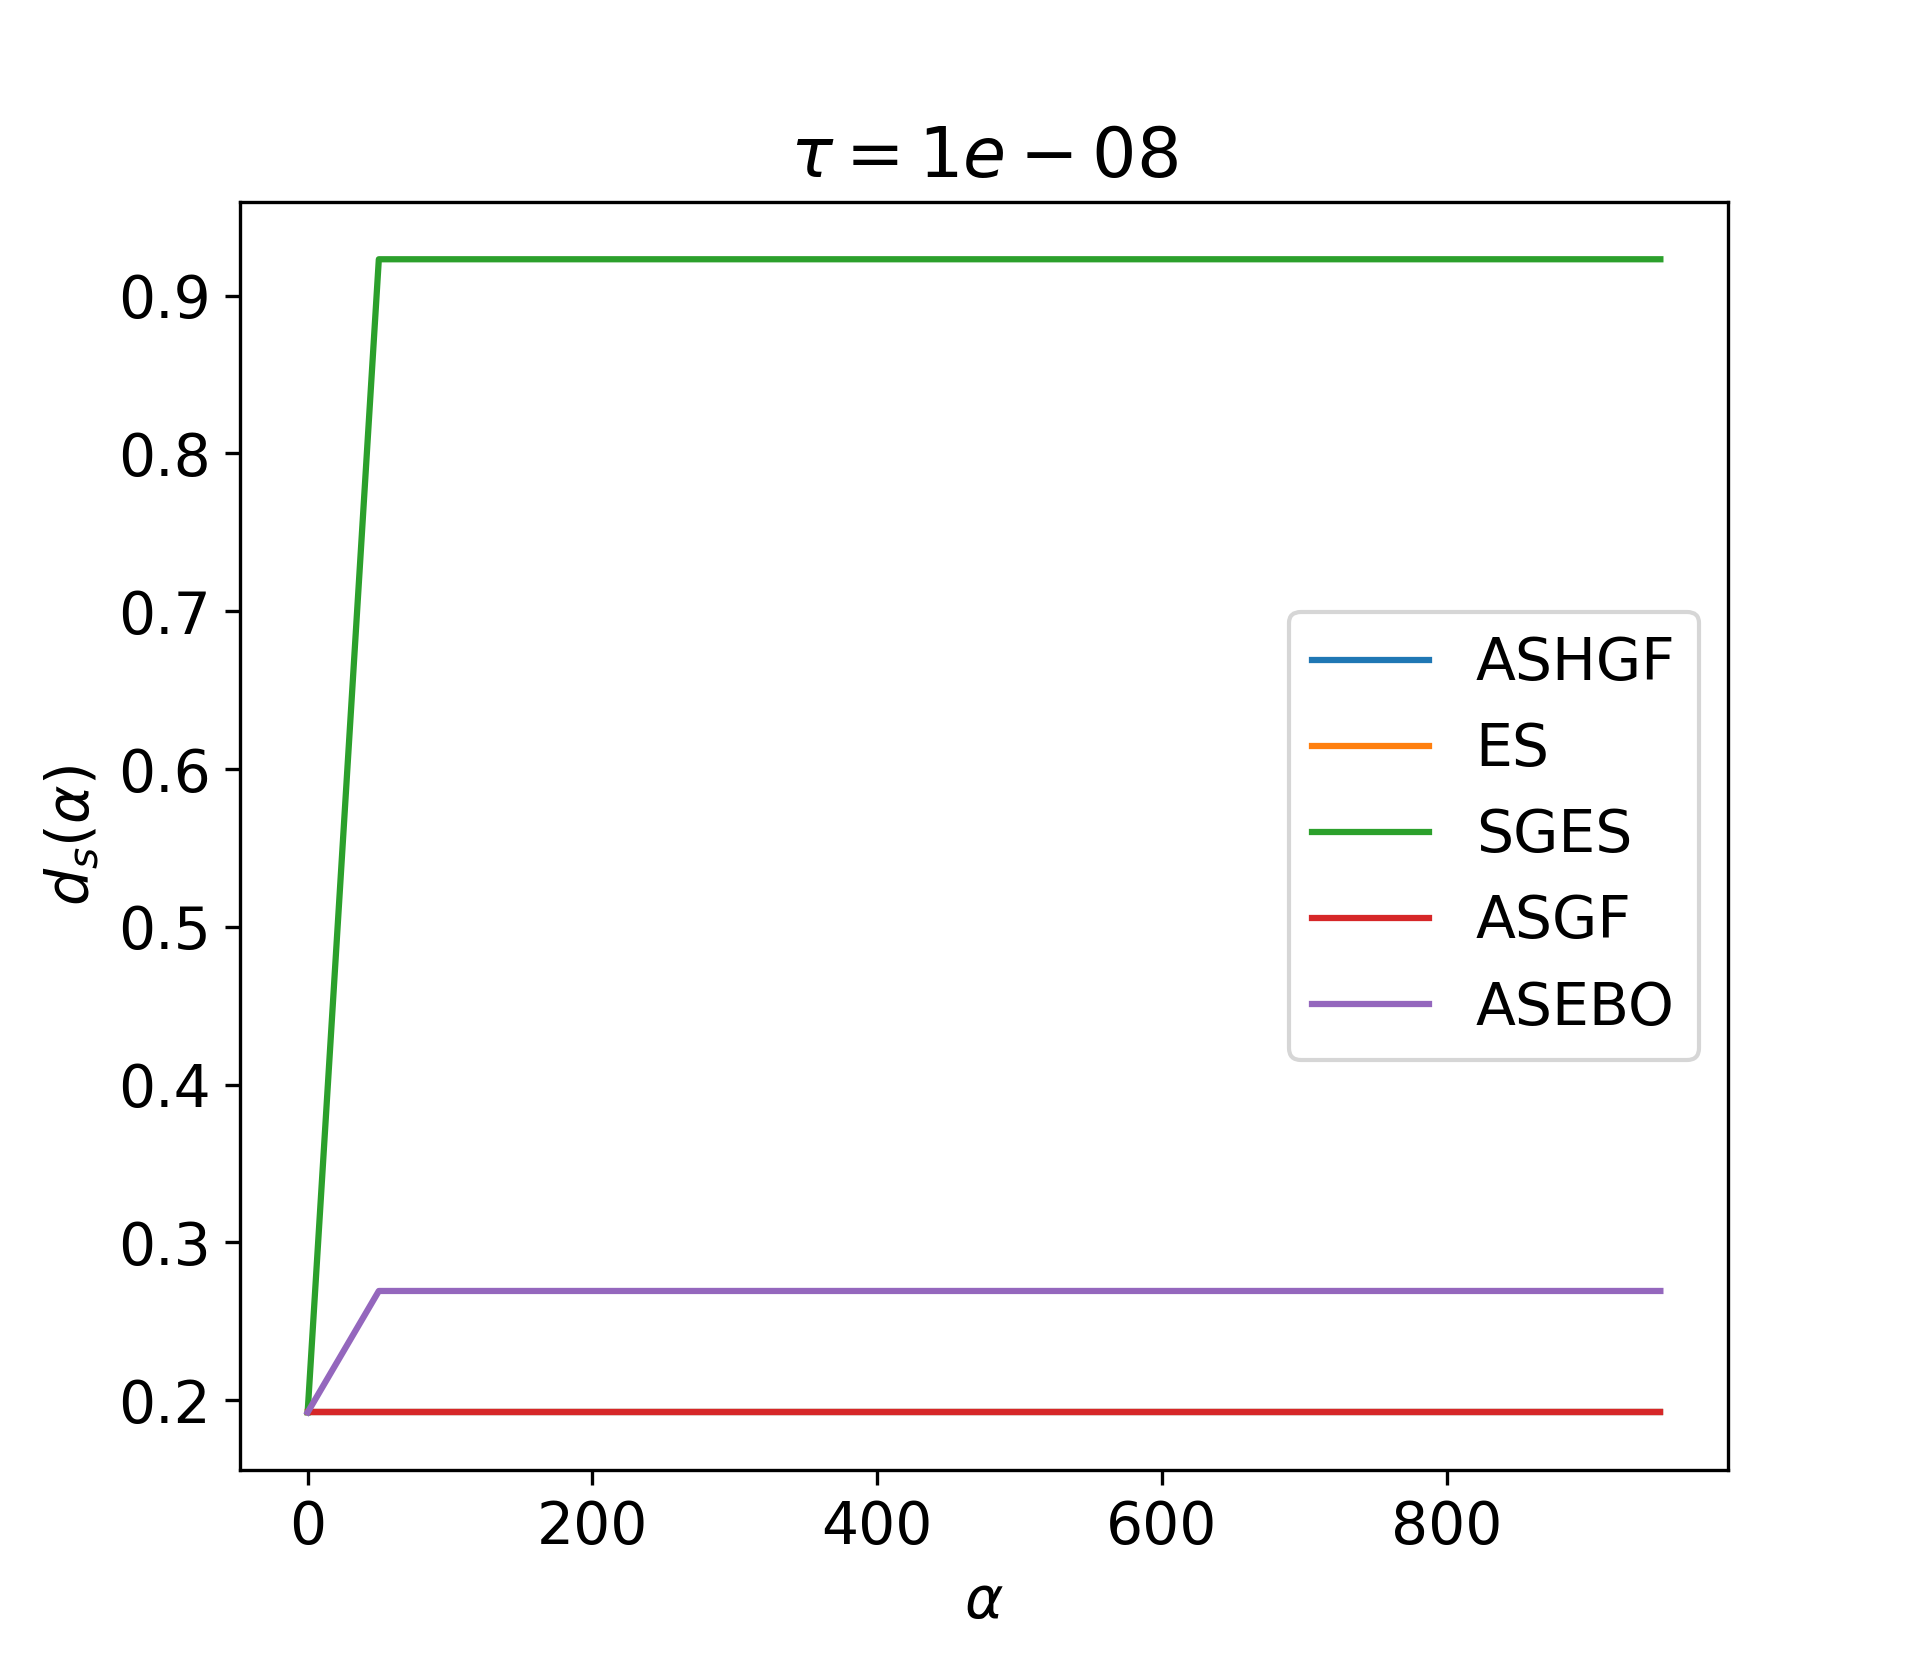
\includegraphics[width=1\textwidth]{figures/data_profiles/1000/data_profile_1000_10000_1e-08.png}
\end{subfigure}%
\begin{subfigure}{0.3\textwidth}
  \centering 
  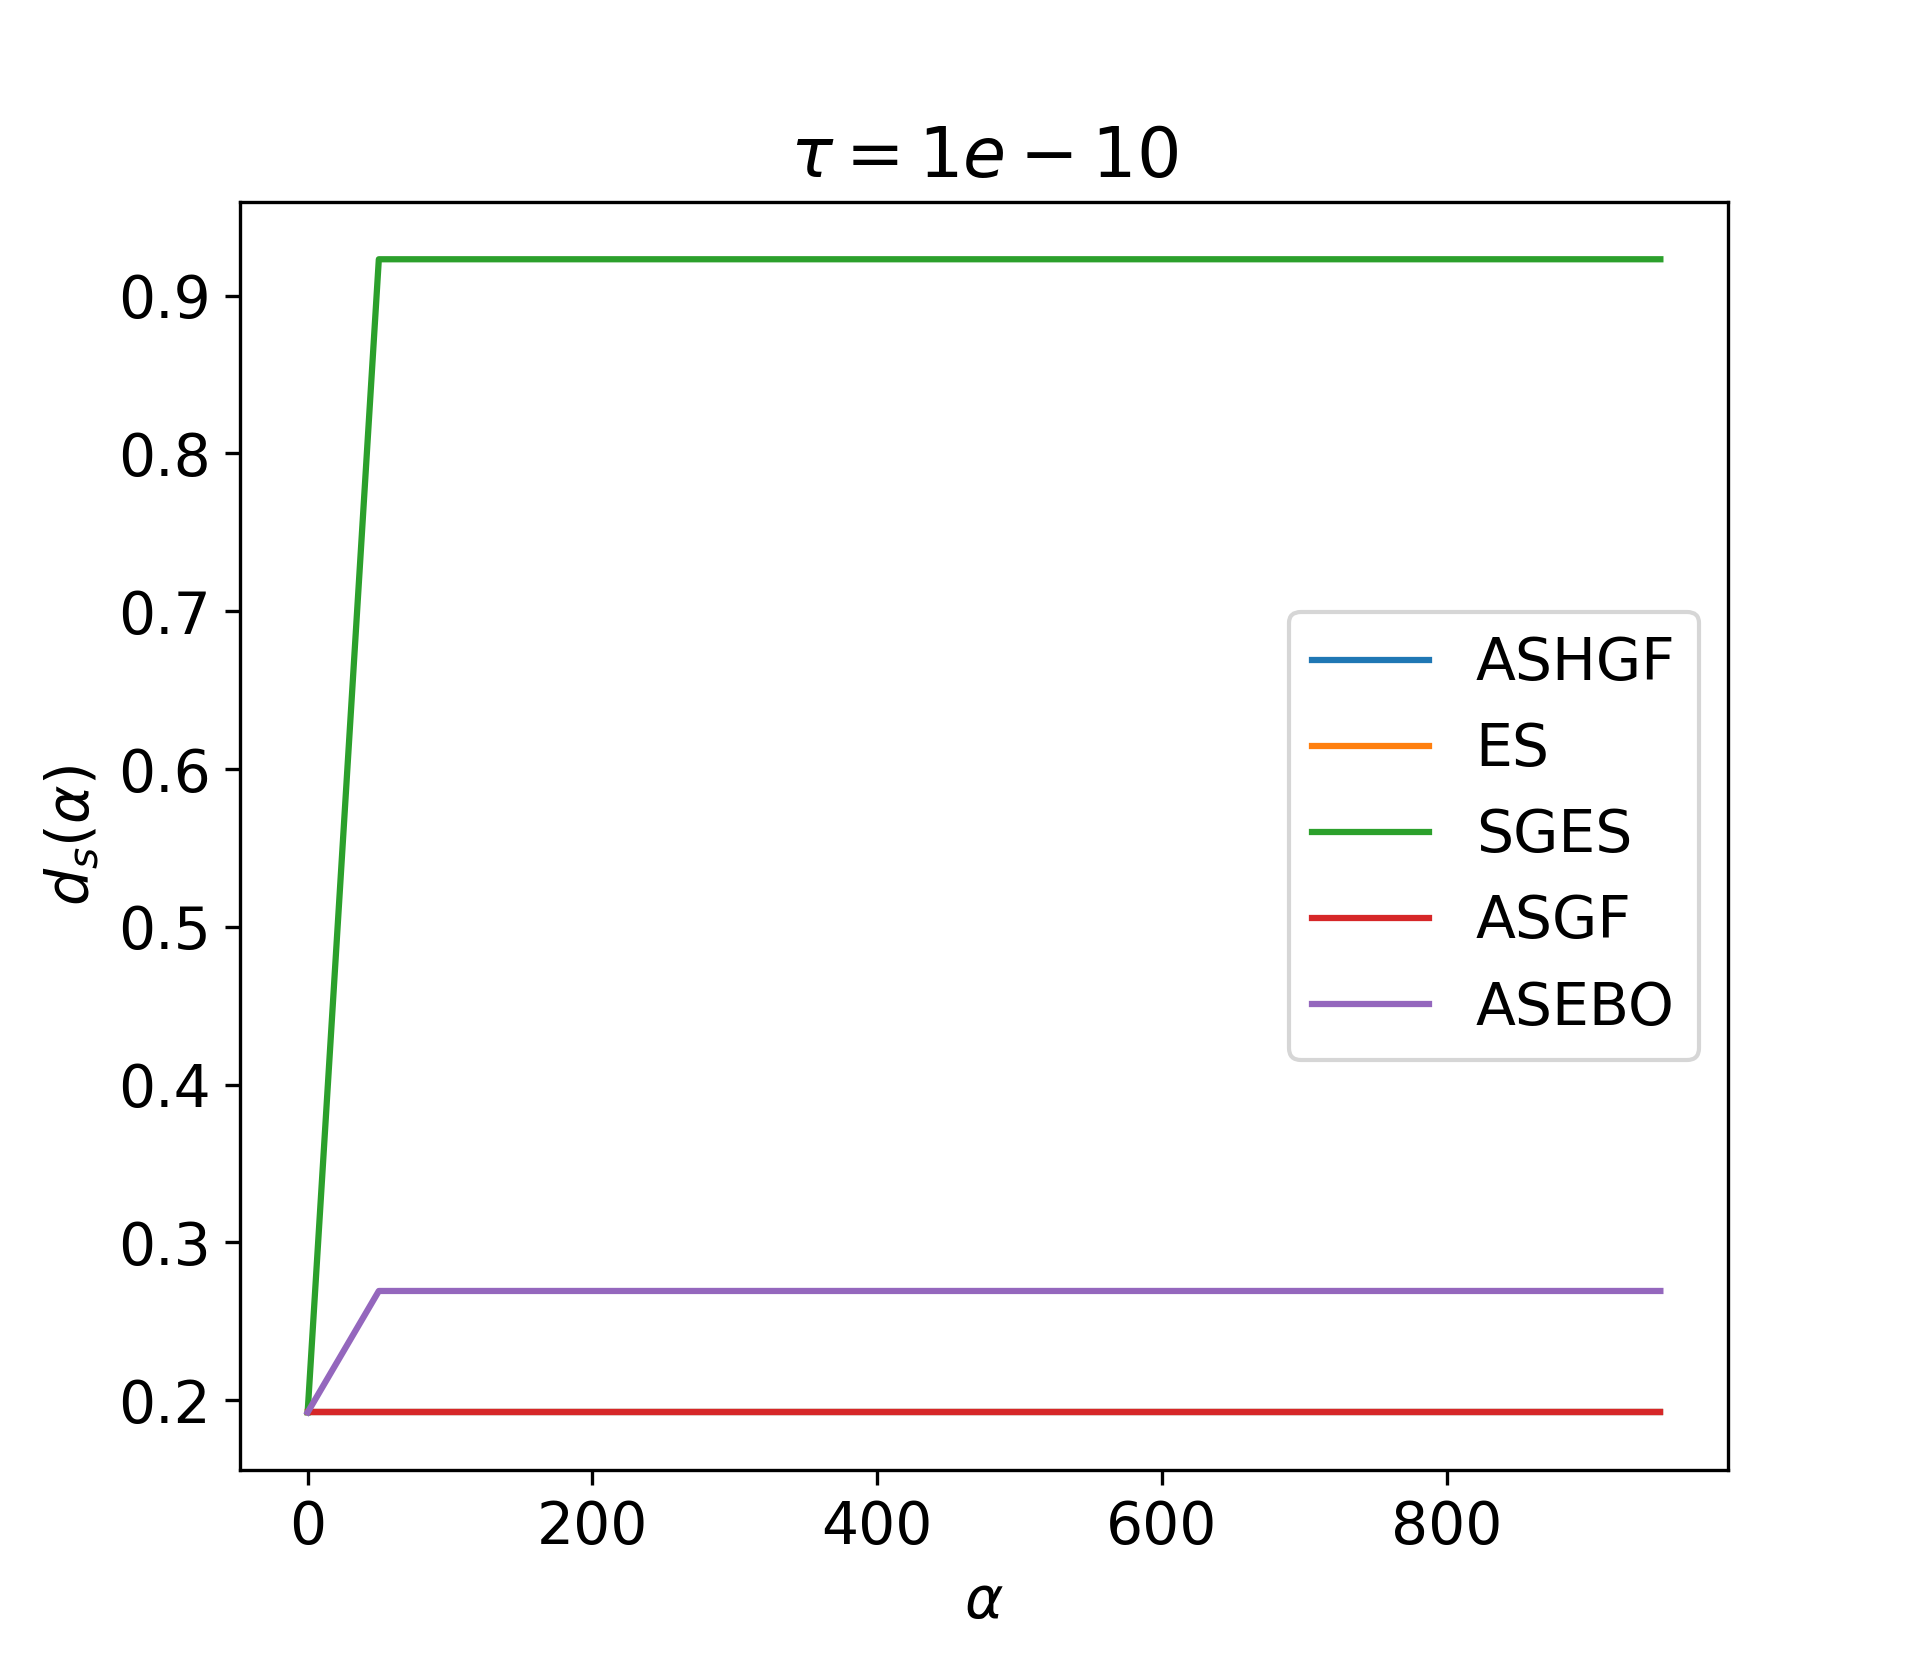
\includegraphics[width=1\textwidth]{figures/data_profiles/1000/data_profile_1000_10000_1e-10.png}
\end{subfigure}
\caption{Data profiles with $\mu_L = 10^{4}$}
\label{DataProfiles1000Mu10000}
\end{figure}

\begin{figure}[H]
\centering
\begin{subfigure}{0.3\textwidth}
  \centering 
  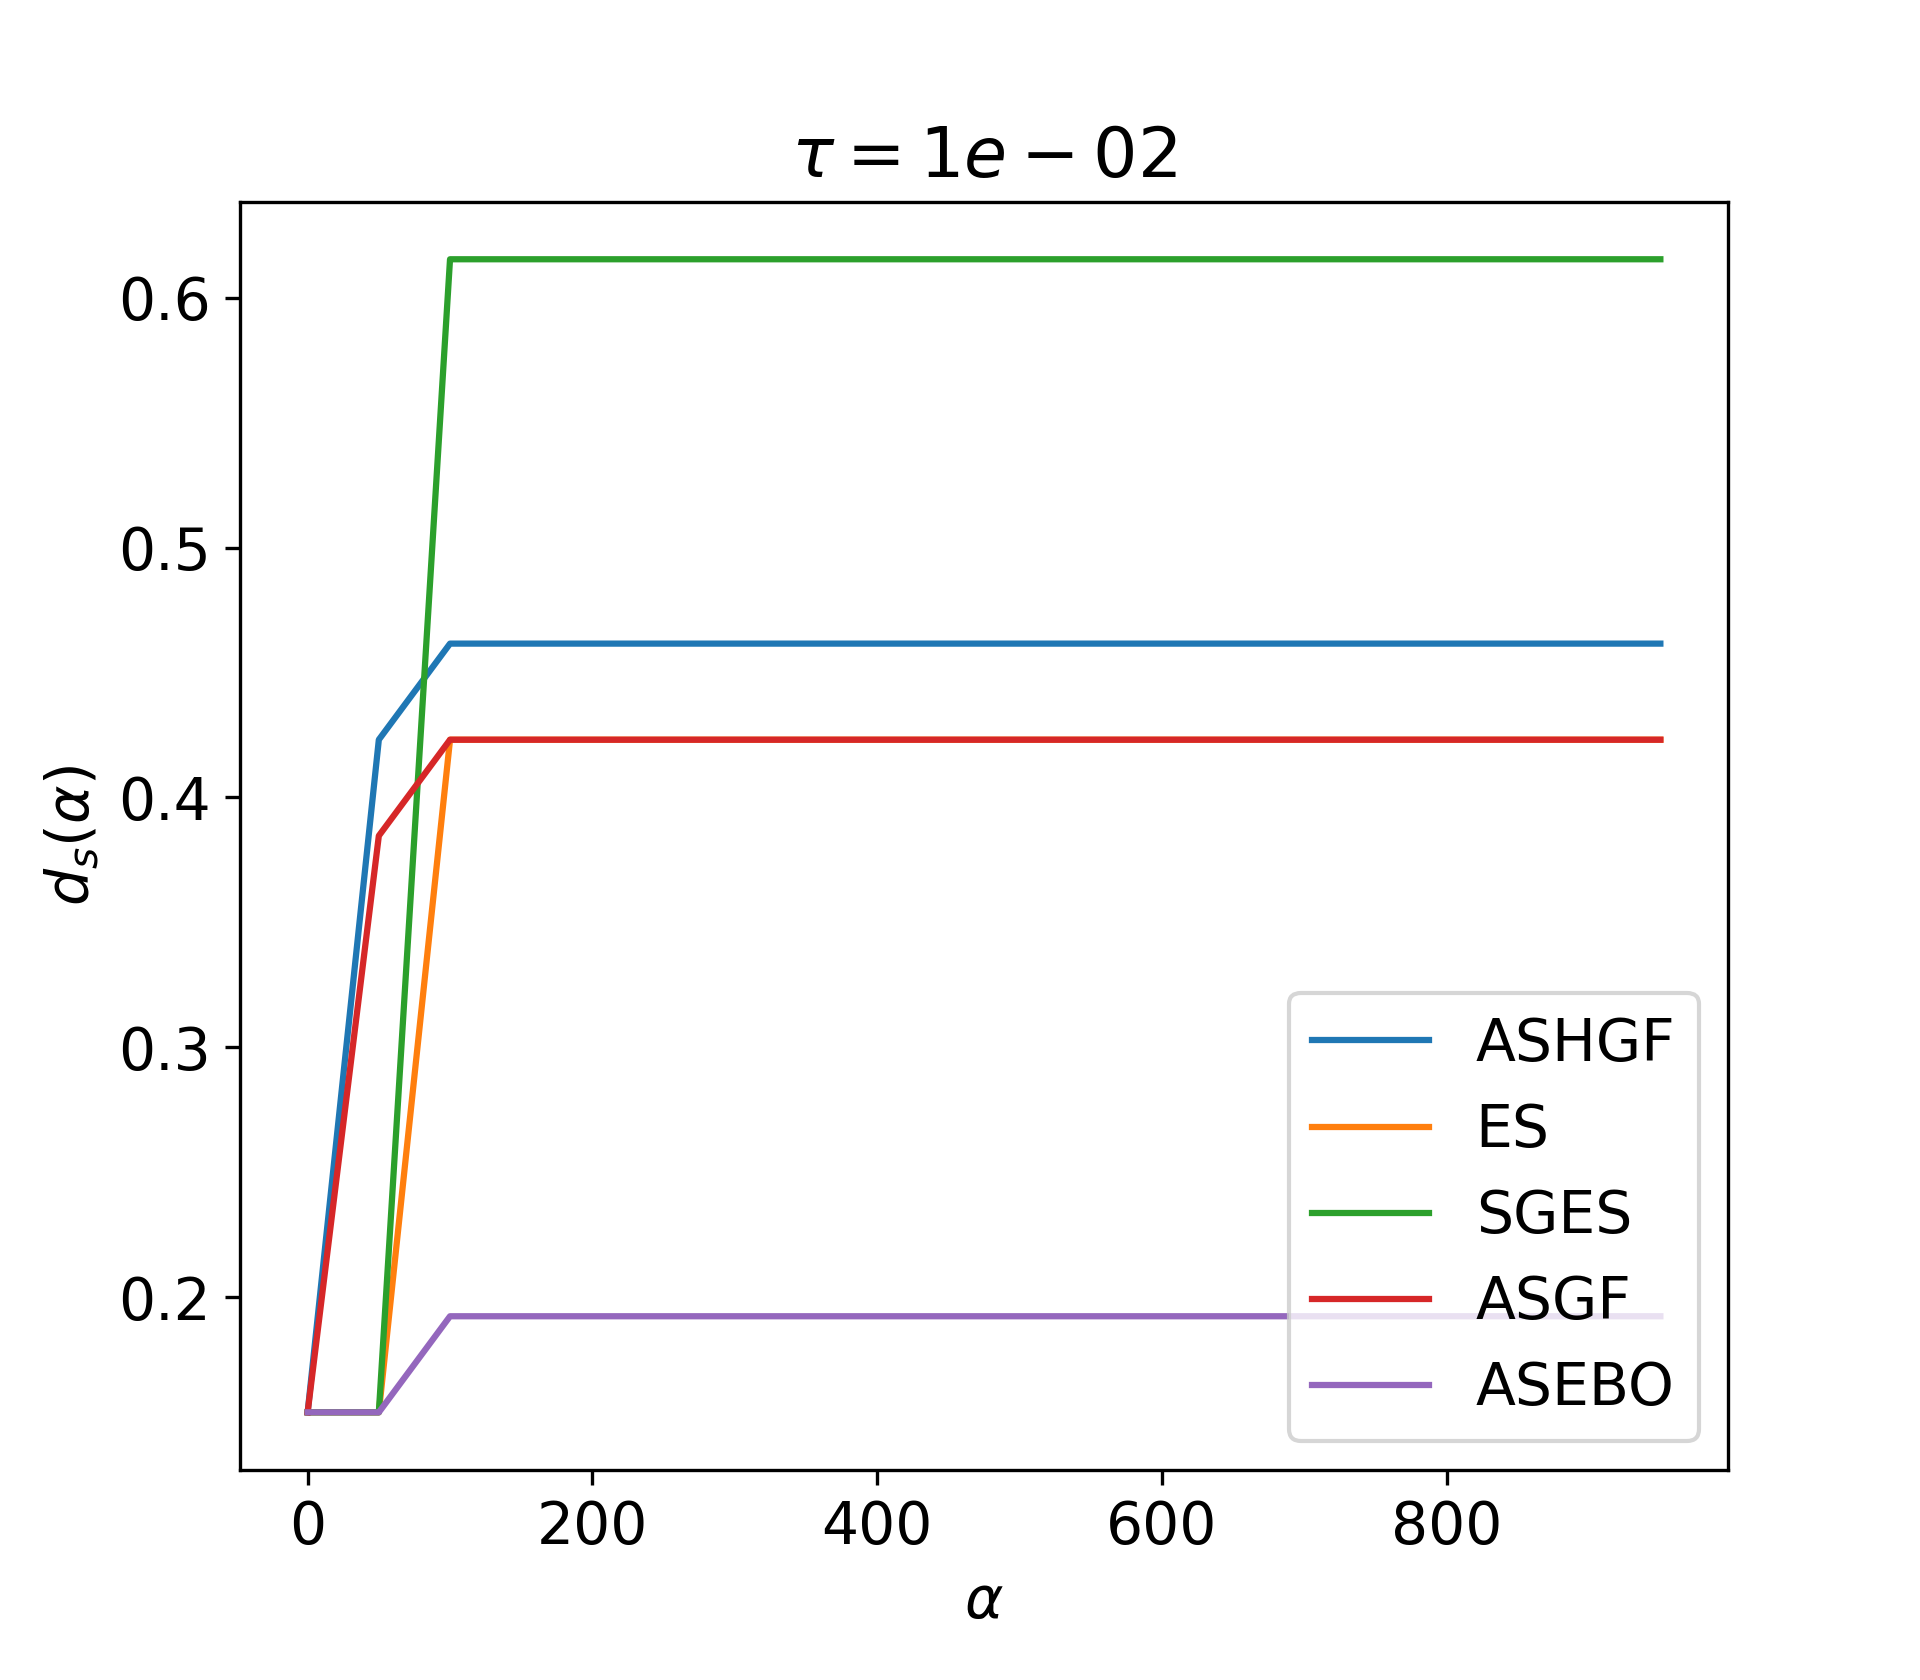
\includegraphics[width=1\textwidth]{figures/data_profiles/1000/data_profile_1000_100000_1e-02.png}
\end{subfigure}%
\begin{subfigure}{0.3\textwidth}
  \centering 
  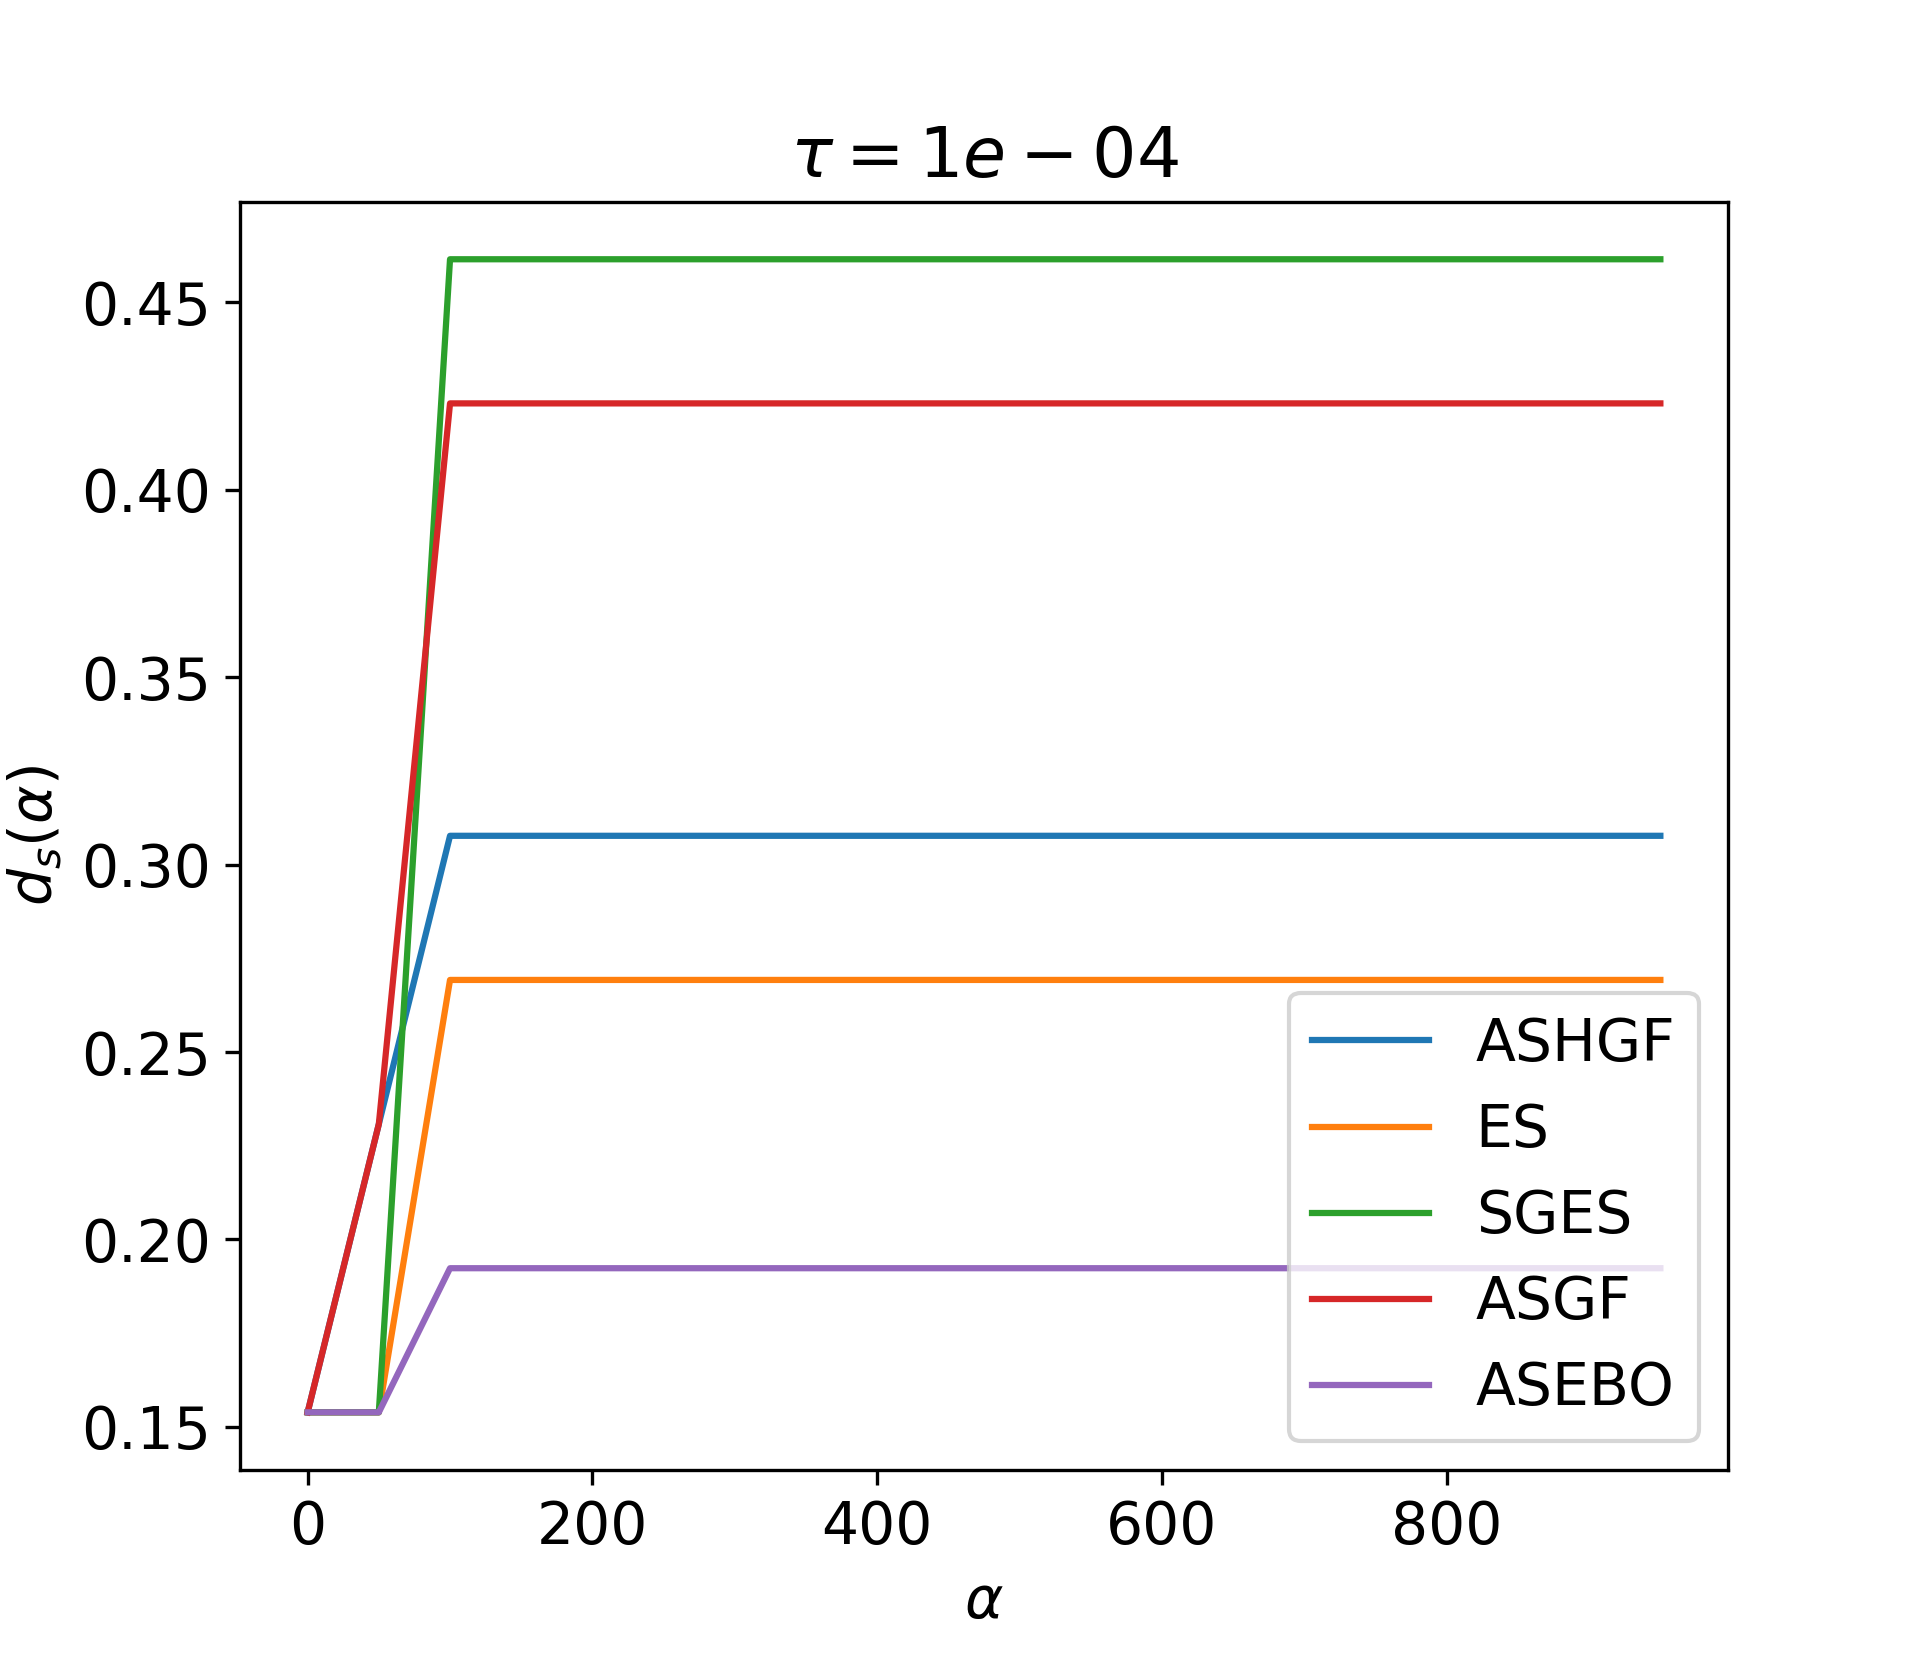
\includegraphics[width=1\textwidth]{figures/data_profiles/1000/data_profile_1000_100000_1e-04.png}
\end{subfigure}
\begin{subfigure}{0.3\textwidth}
  \centering 
  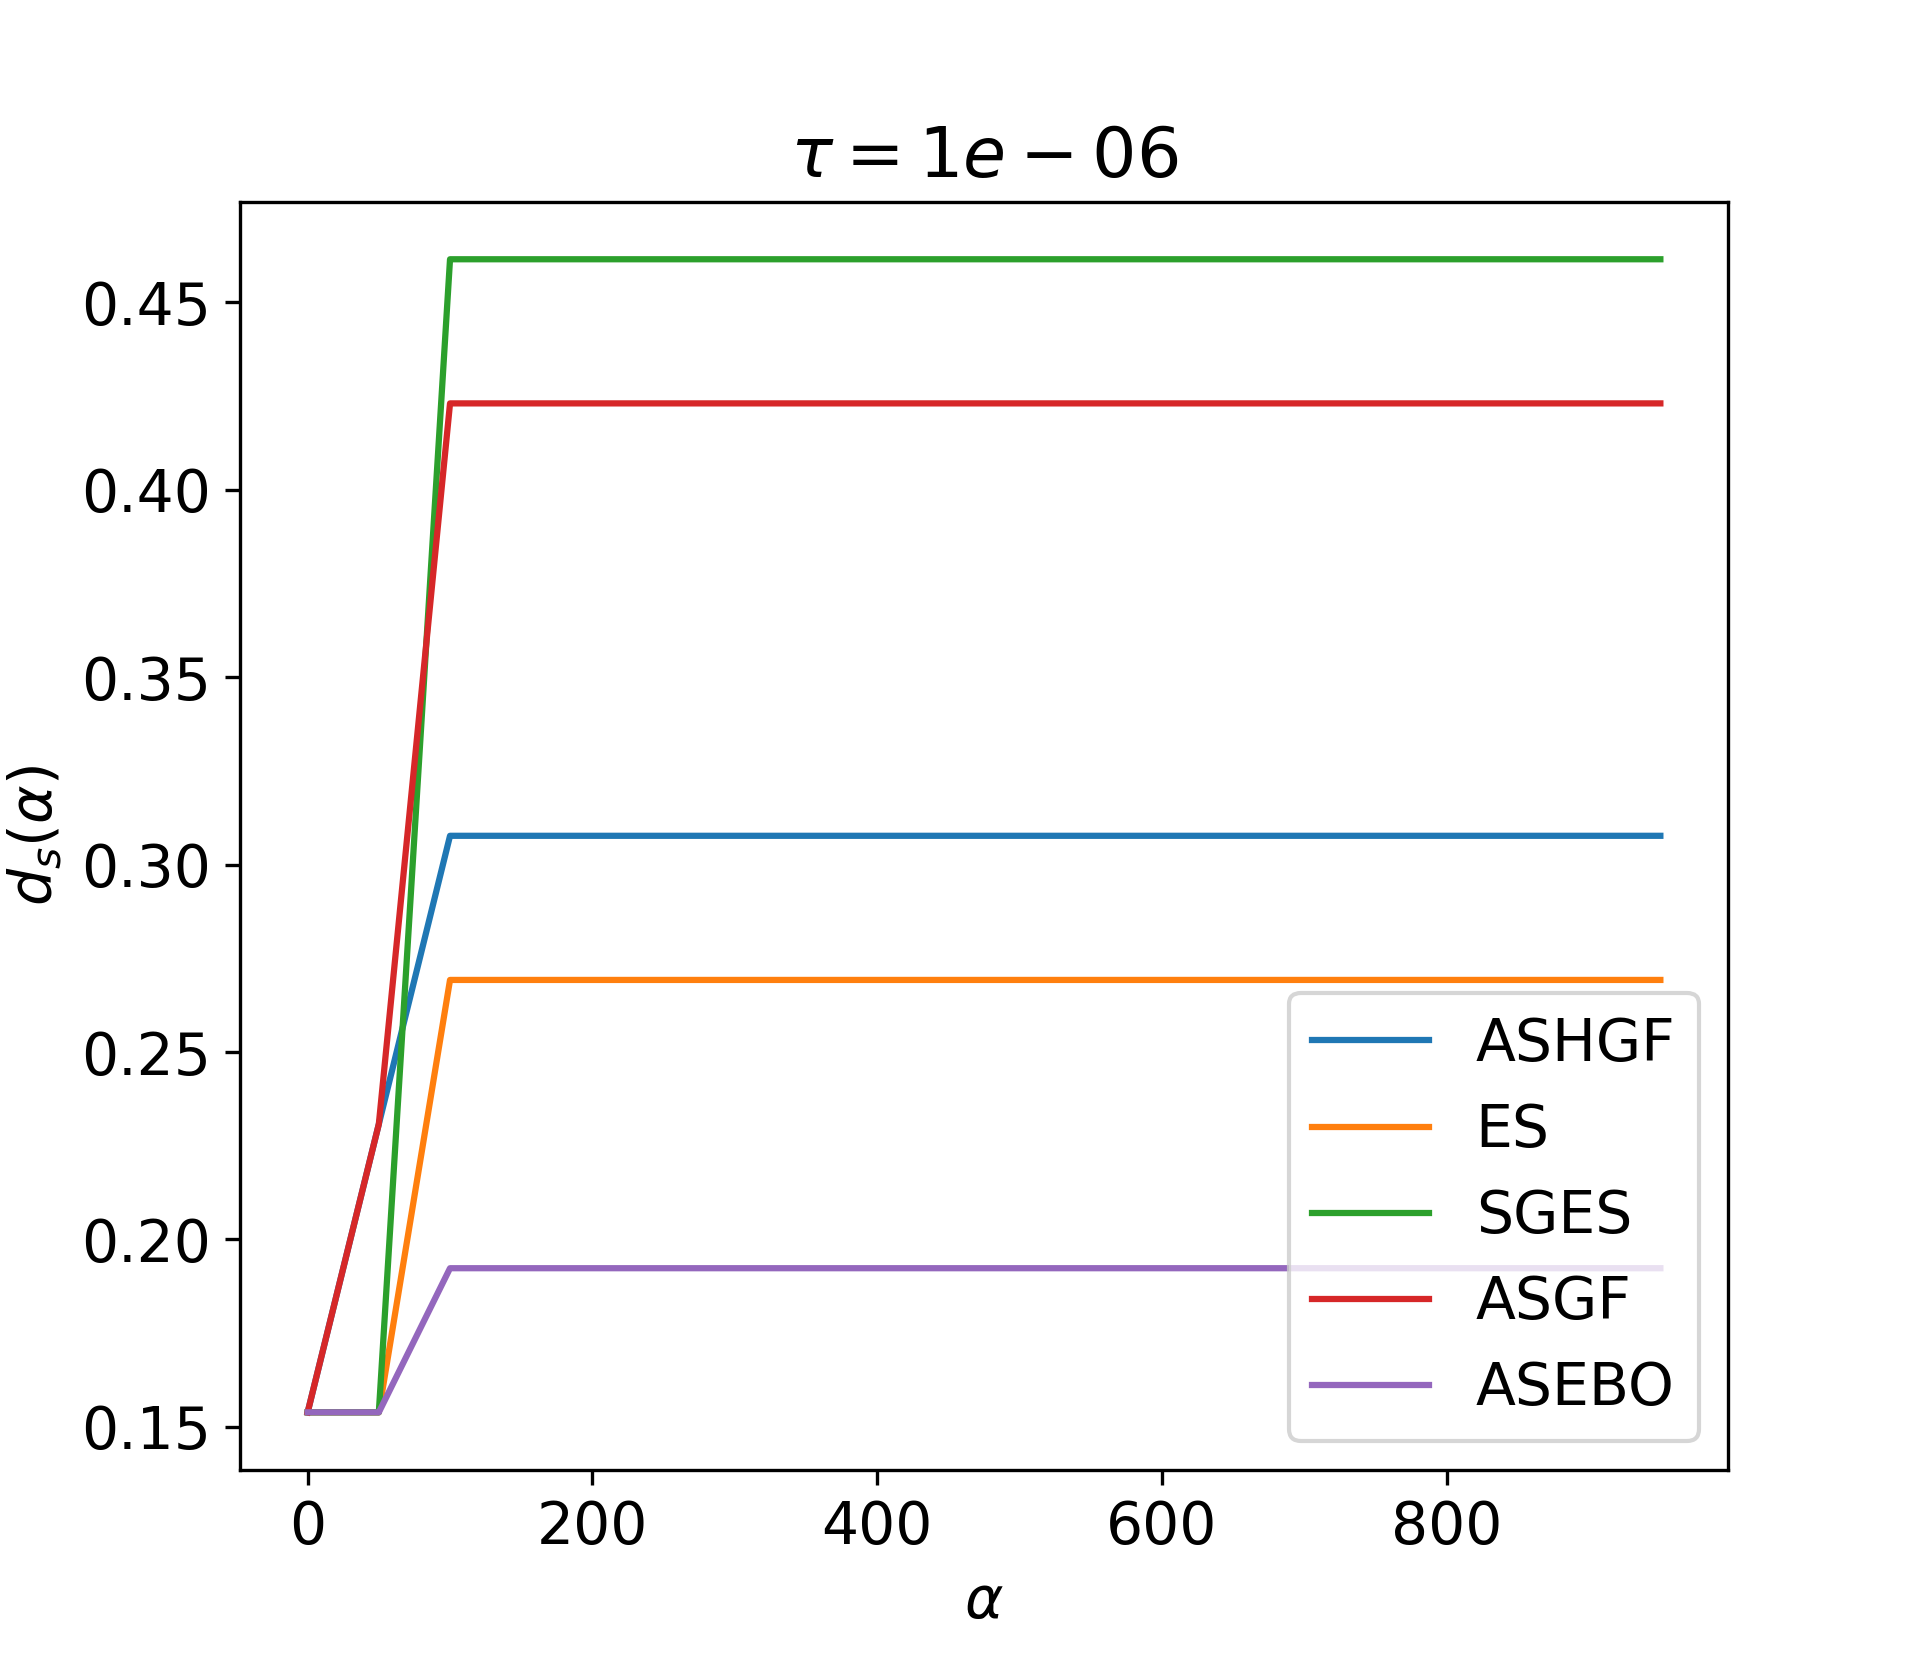
\includegraphics[width=1\textwidth]{figures/data_profiles/1000/data_profile_1000_100000_1e-06.png}
\end{subfigure}
\centering
\begin{subfigure}{0.3\textwidth}
  \centering 
  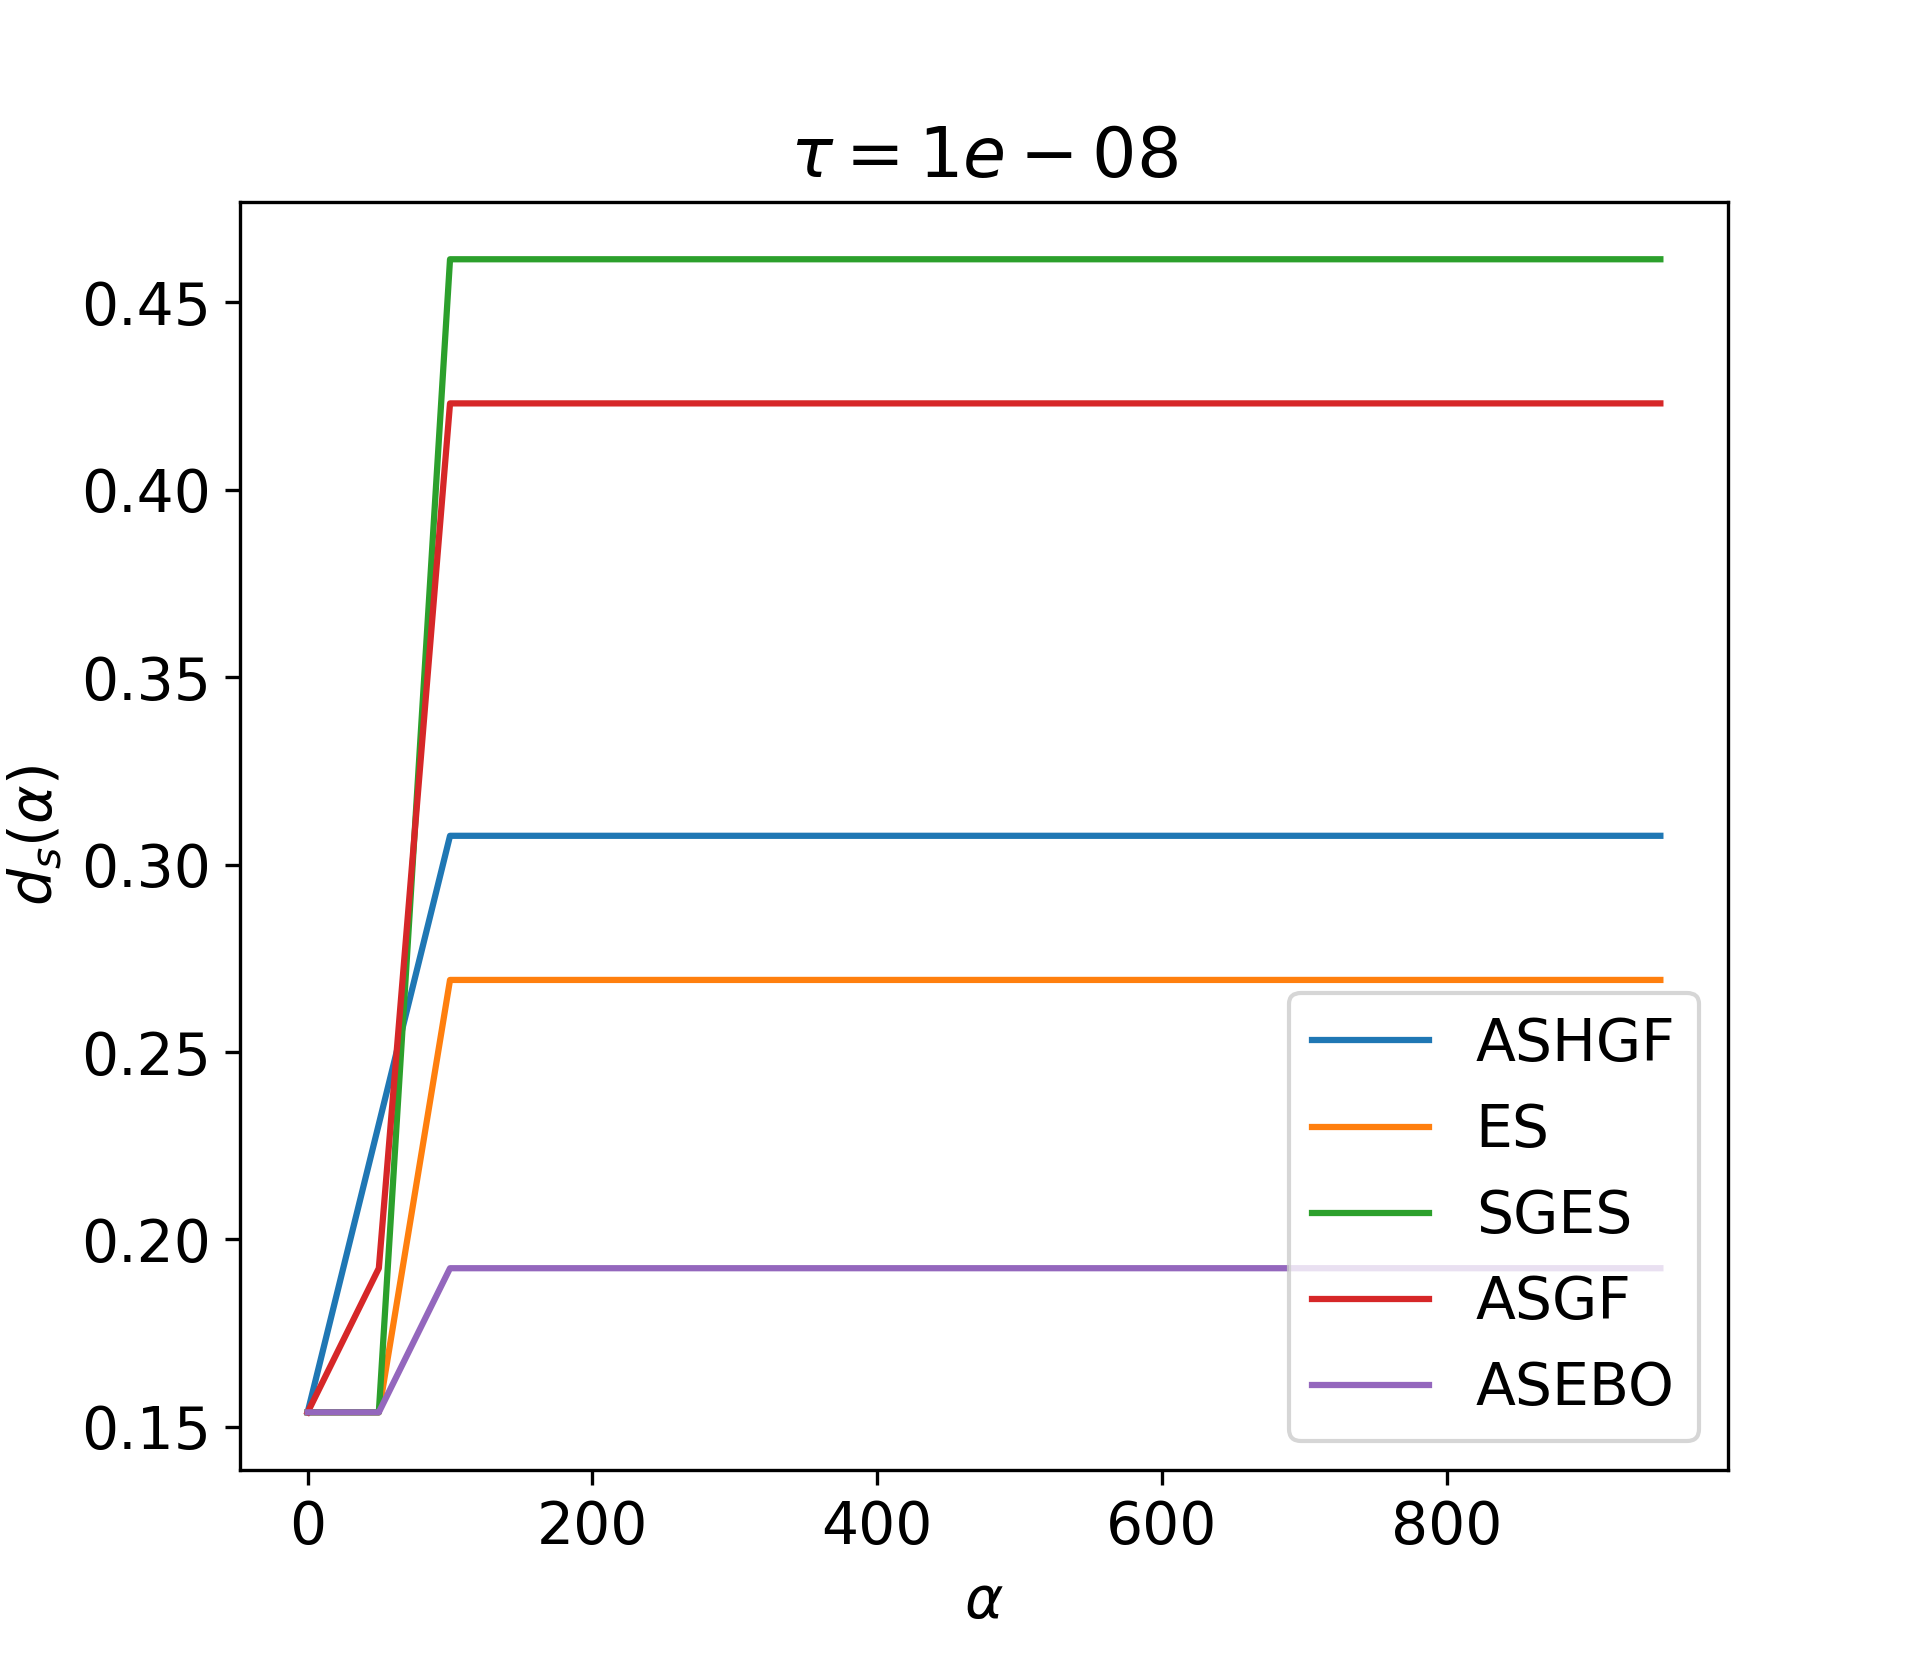
\includegraphics[width=1\textwidth]{figures/data_profiles/1000/data_profile_1000_100000_1e-08.png}
\end{subfigure}%
\begin{subfigure}{0.3\textwidth}
  \centering 
  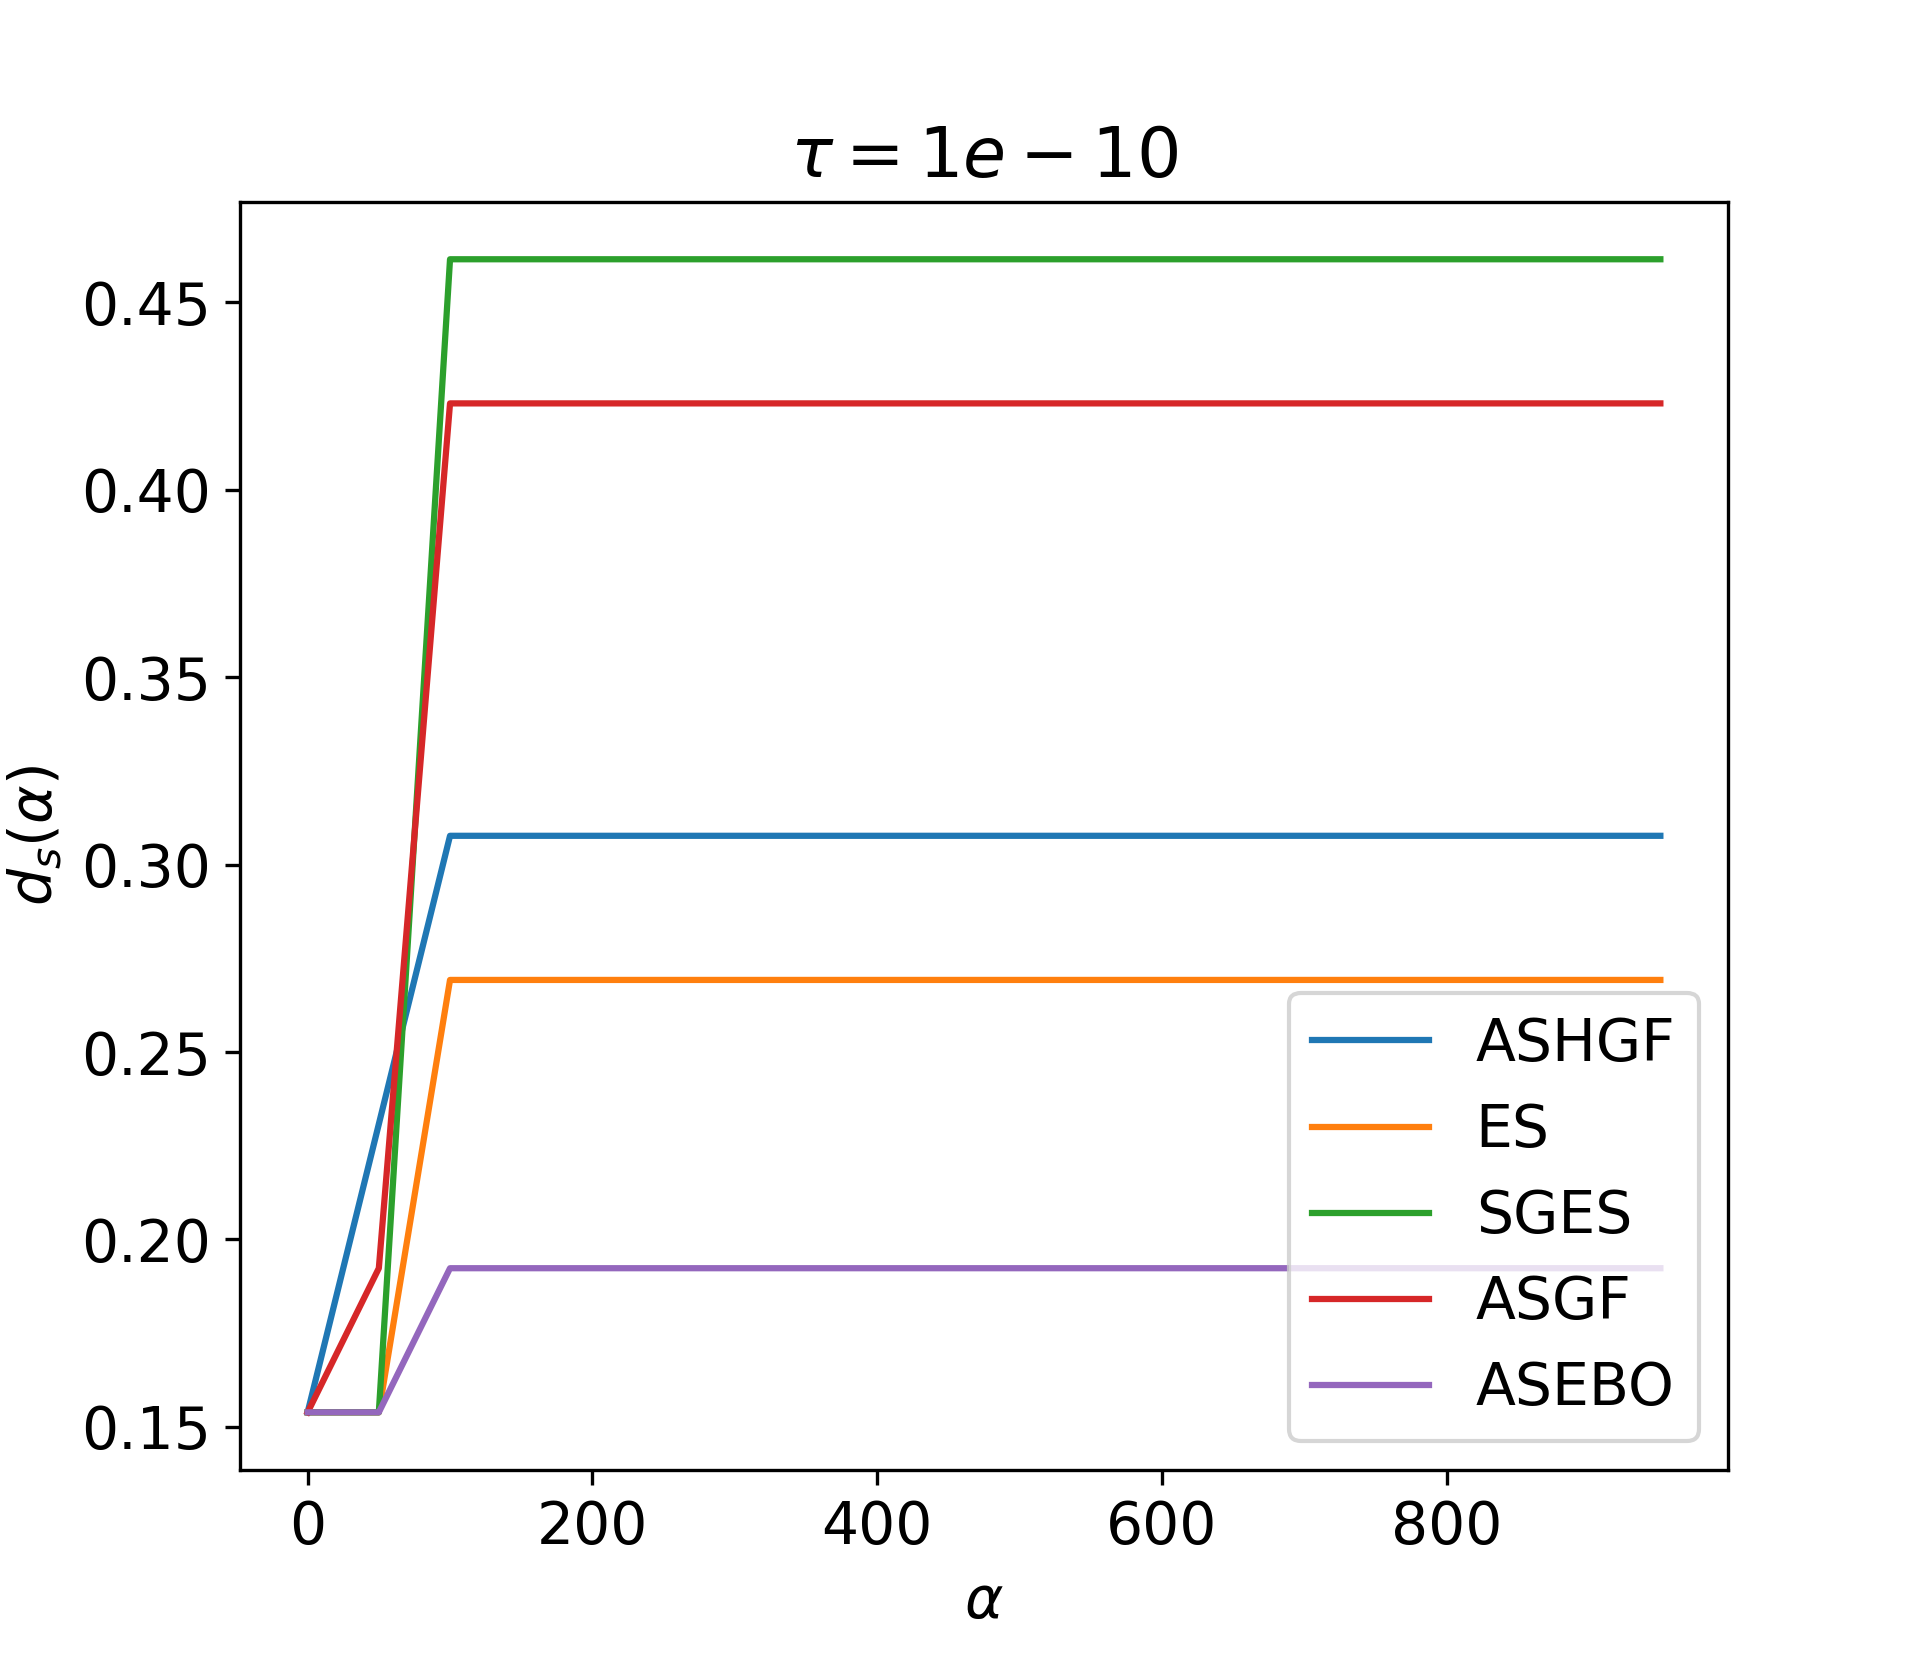
\includegraphics[width=1\textwidth]{figures/data_profiles/1000/data_profile_1000_100000_1e-10.png}
\end{subfigure}
\caption{Data profiles with $\mu_L = 10^{5}$}
\label{DataProfiles1000Mu100000}
\end{figure}

\begin{figure}[H]
\centering
\begin{subfigure}{0.3\textwidth}
  \centering 
  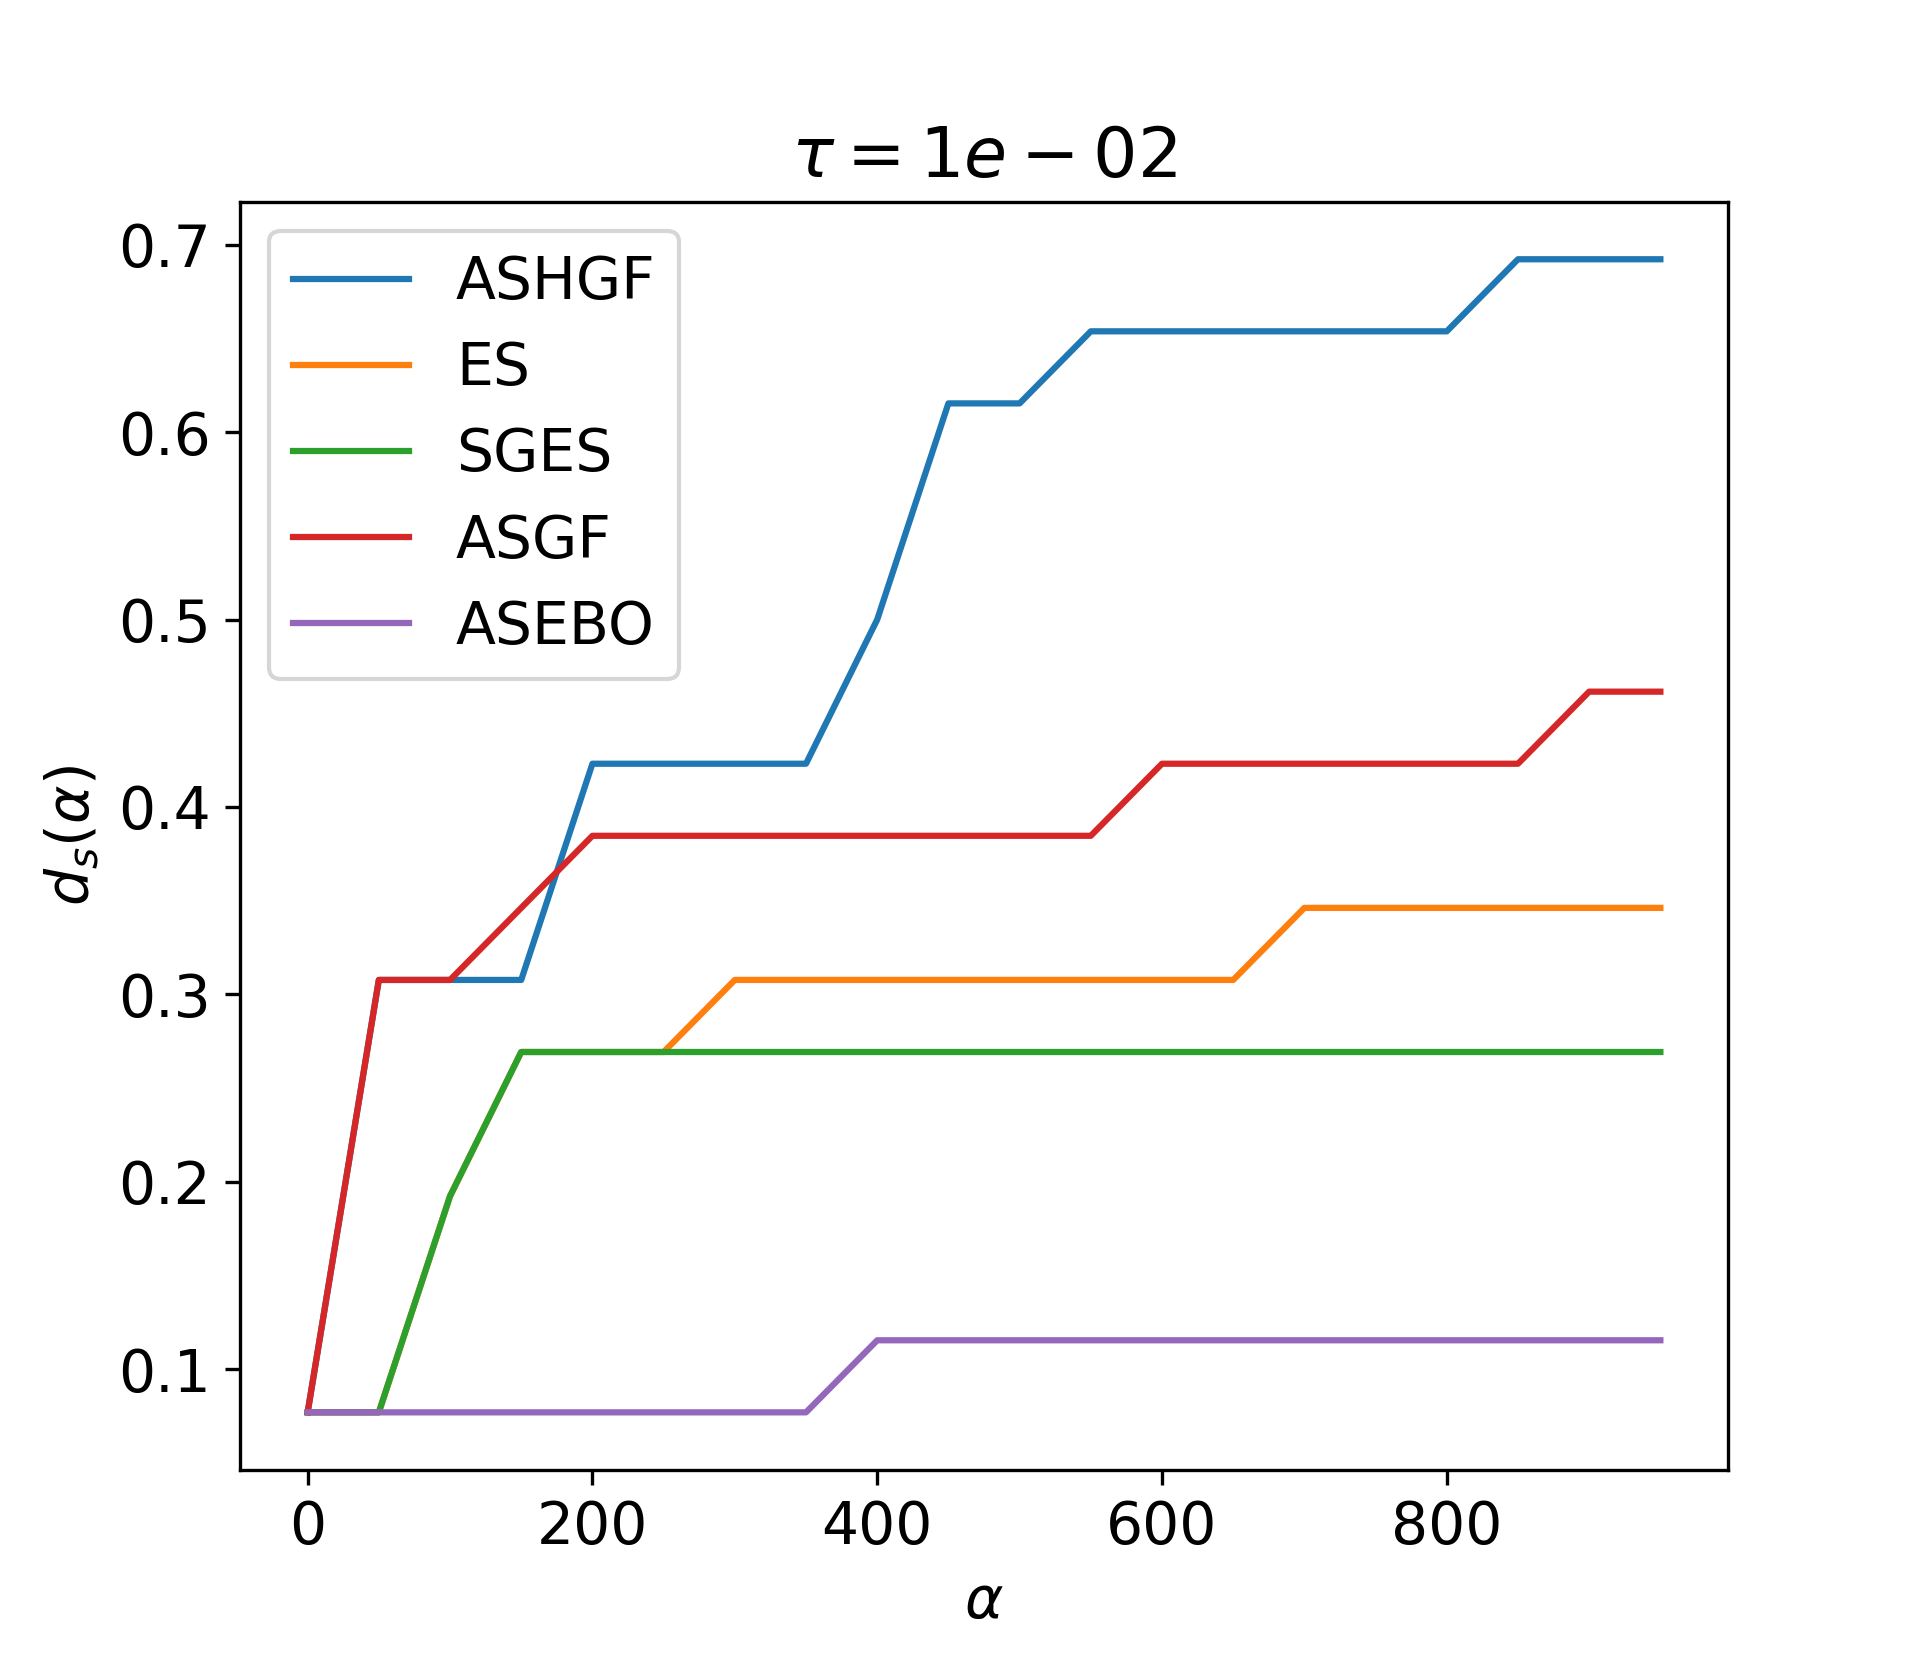
\includegraphics[width=1\textwidth]{figures/data_profiles/1000/data_profile_1000_1000000_1e-02.png}
\end{subfigure}%
\begin{subfigure}{0.3\textwidth}
  \centering 
  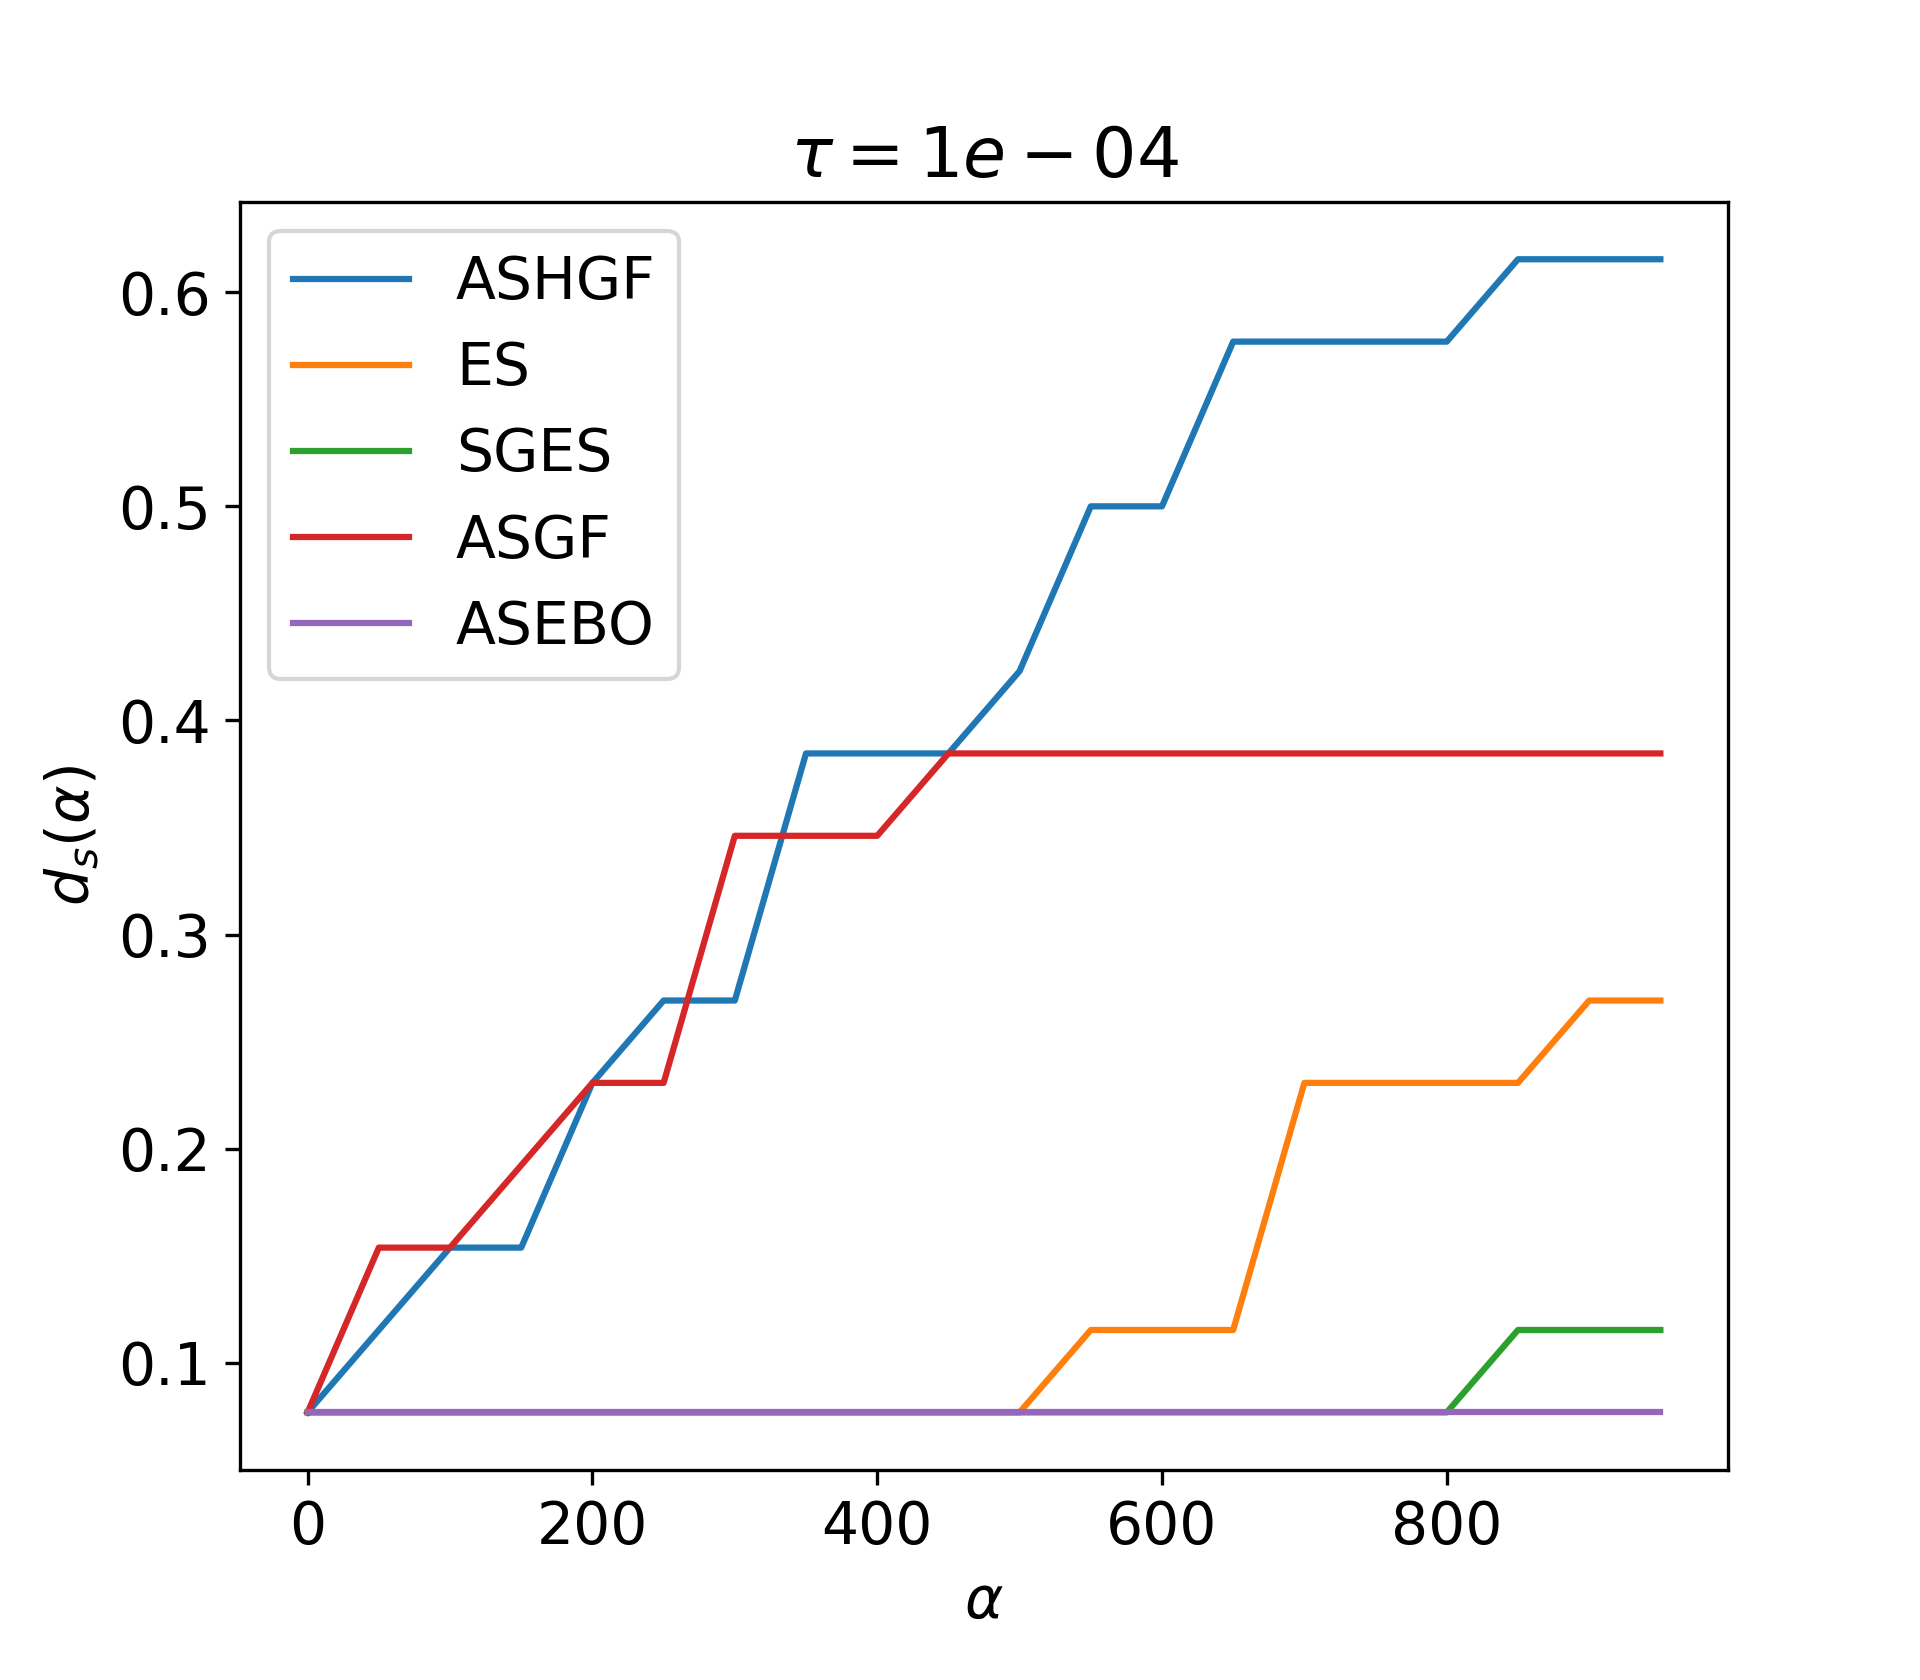
\includegraphics[width=1\textwidth]{figures/data_profiles/1000/data_profile_1000_1000000_1e-04.png}
\end{subfigure}
\begin{subfigure}{0.3\textwidth}
  \centering 
  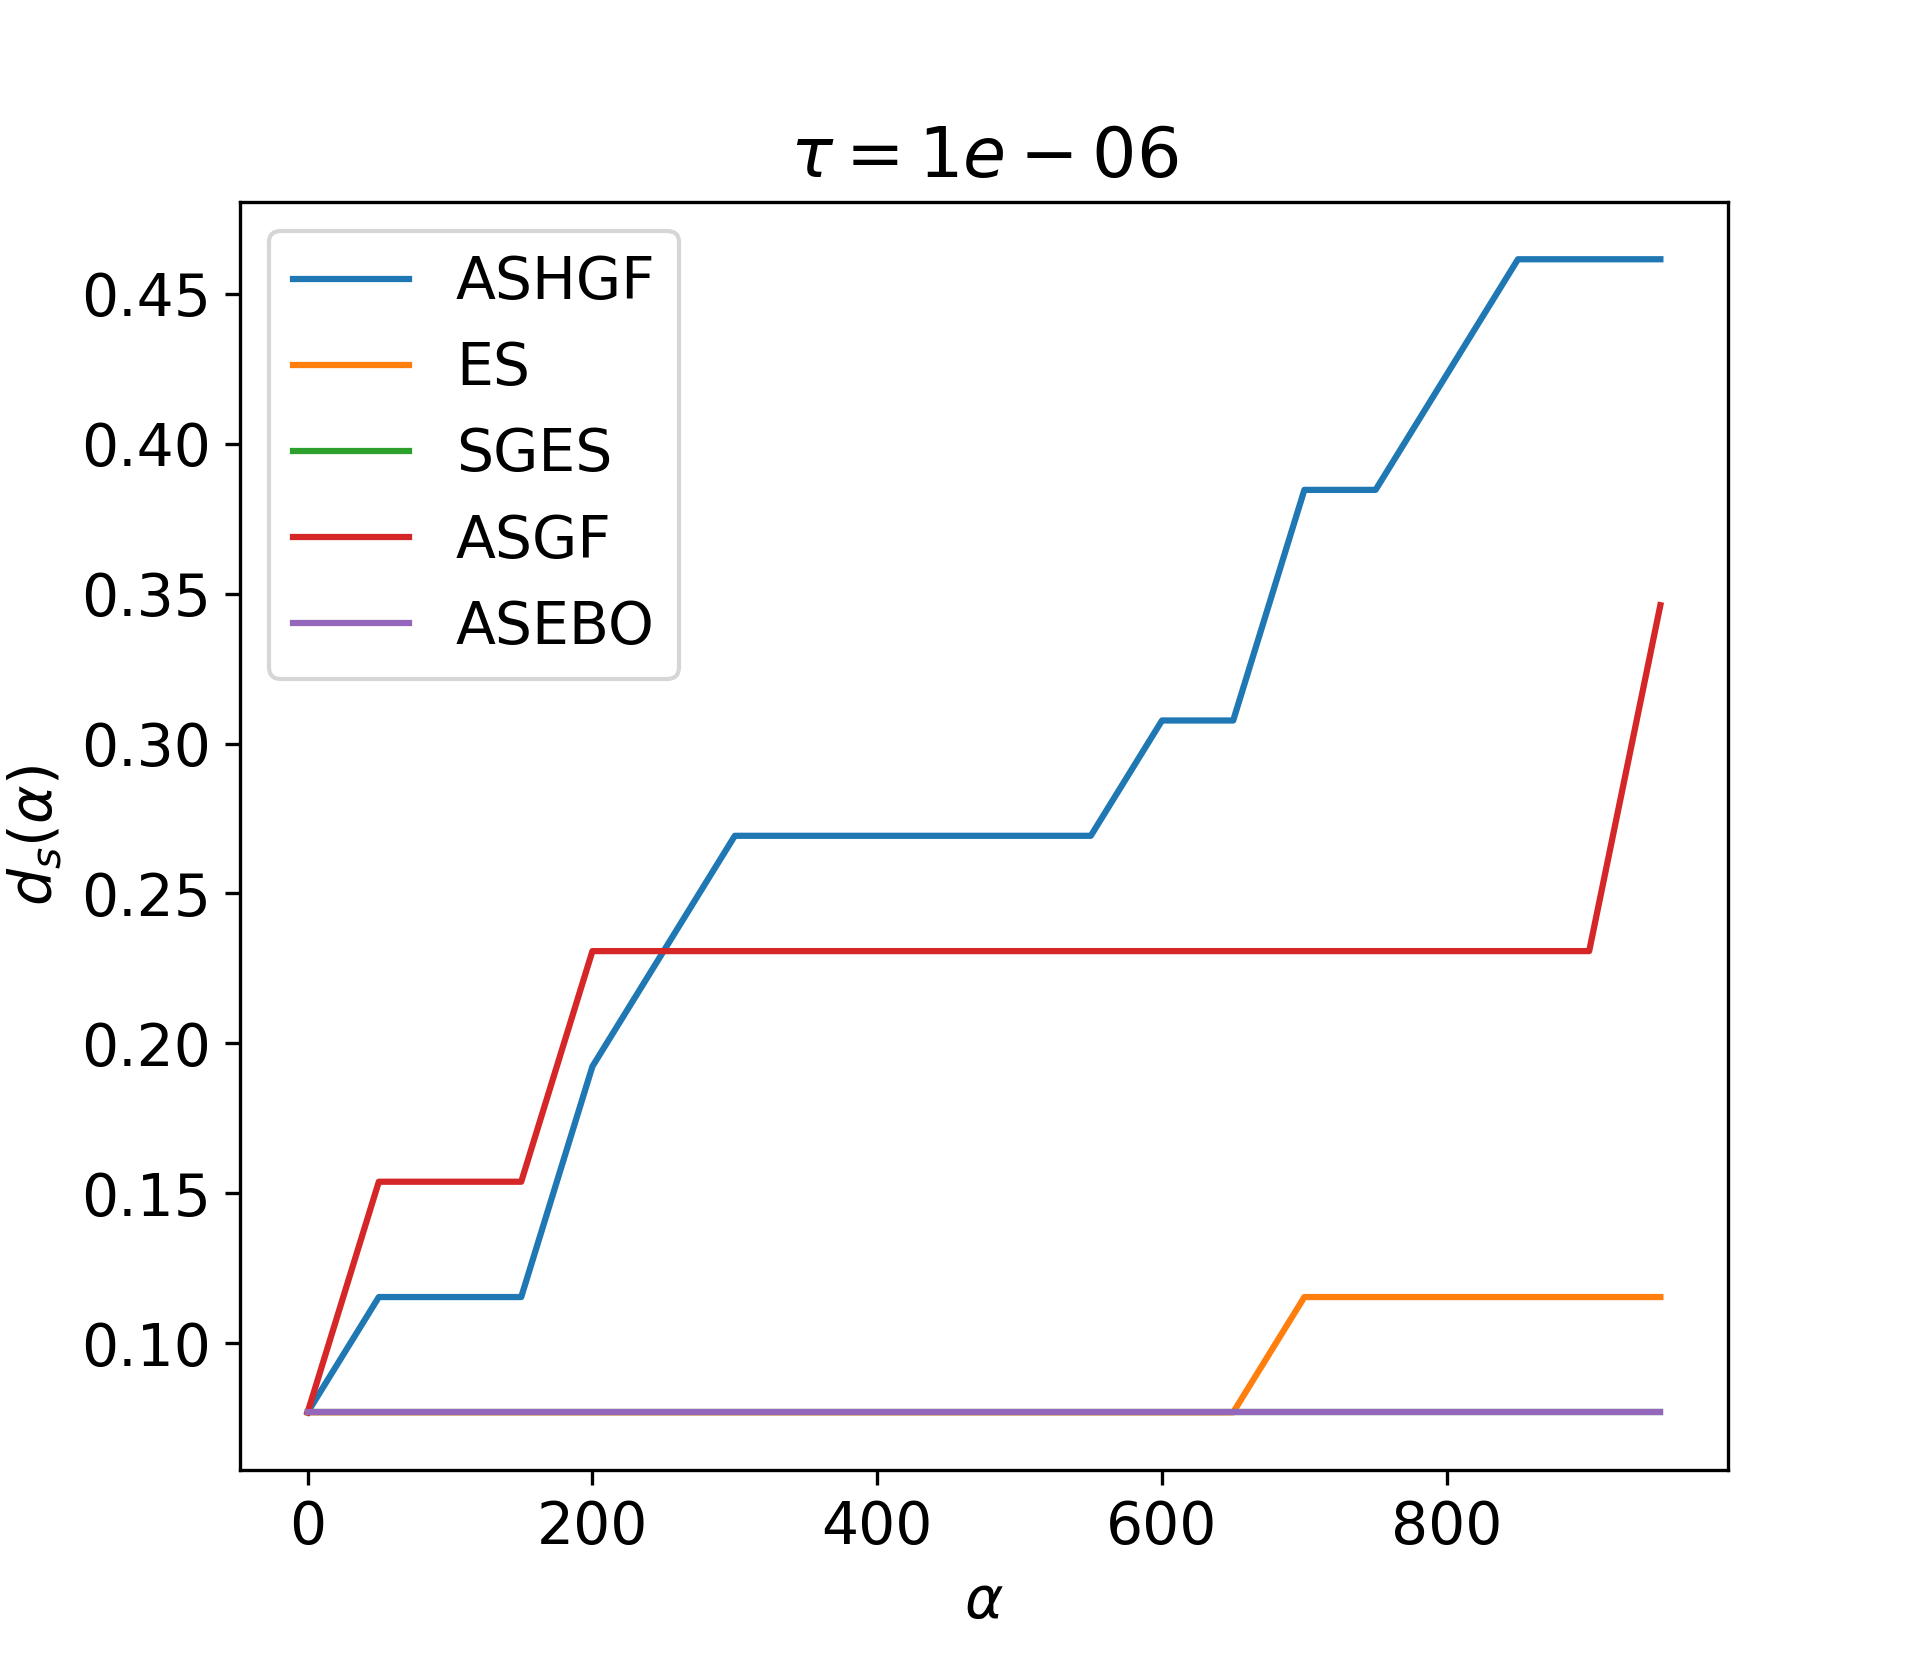
\includegraphics[width=1\textwidth]{figures/data_profiles/1000/data_profile_1000_1000000_1e-06.png}
\end{subfigure}
\centering
\begin{subfigure}{0.3\textwidth}
  \centering 
  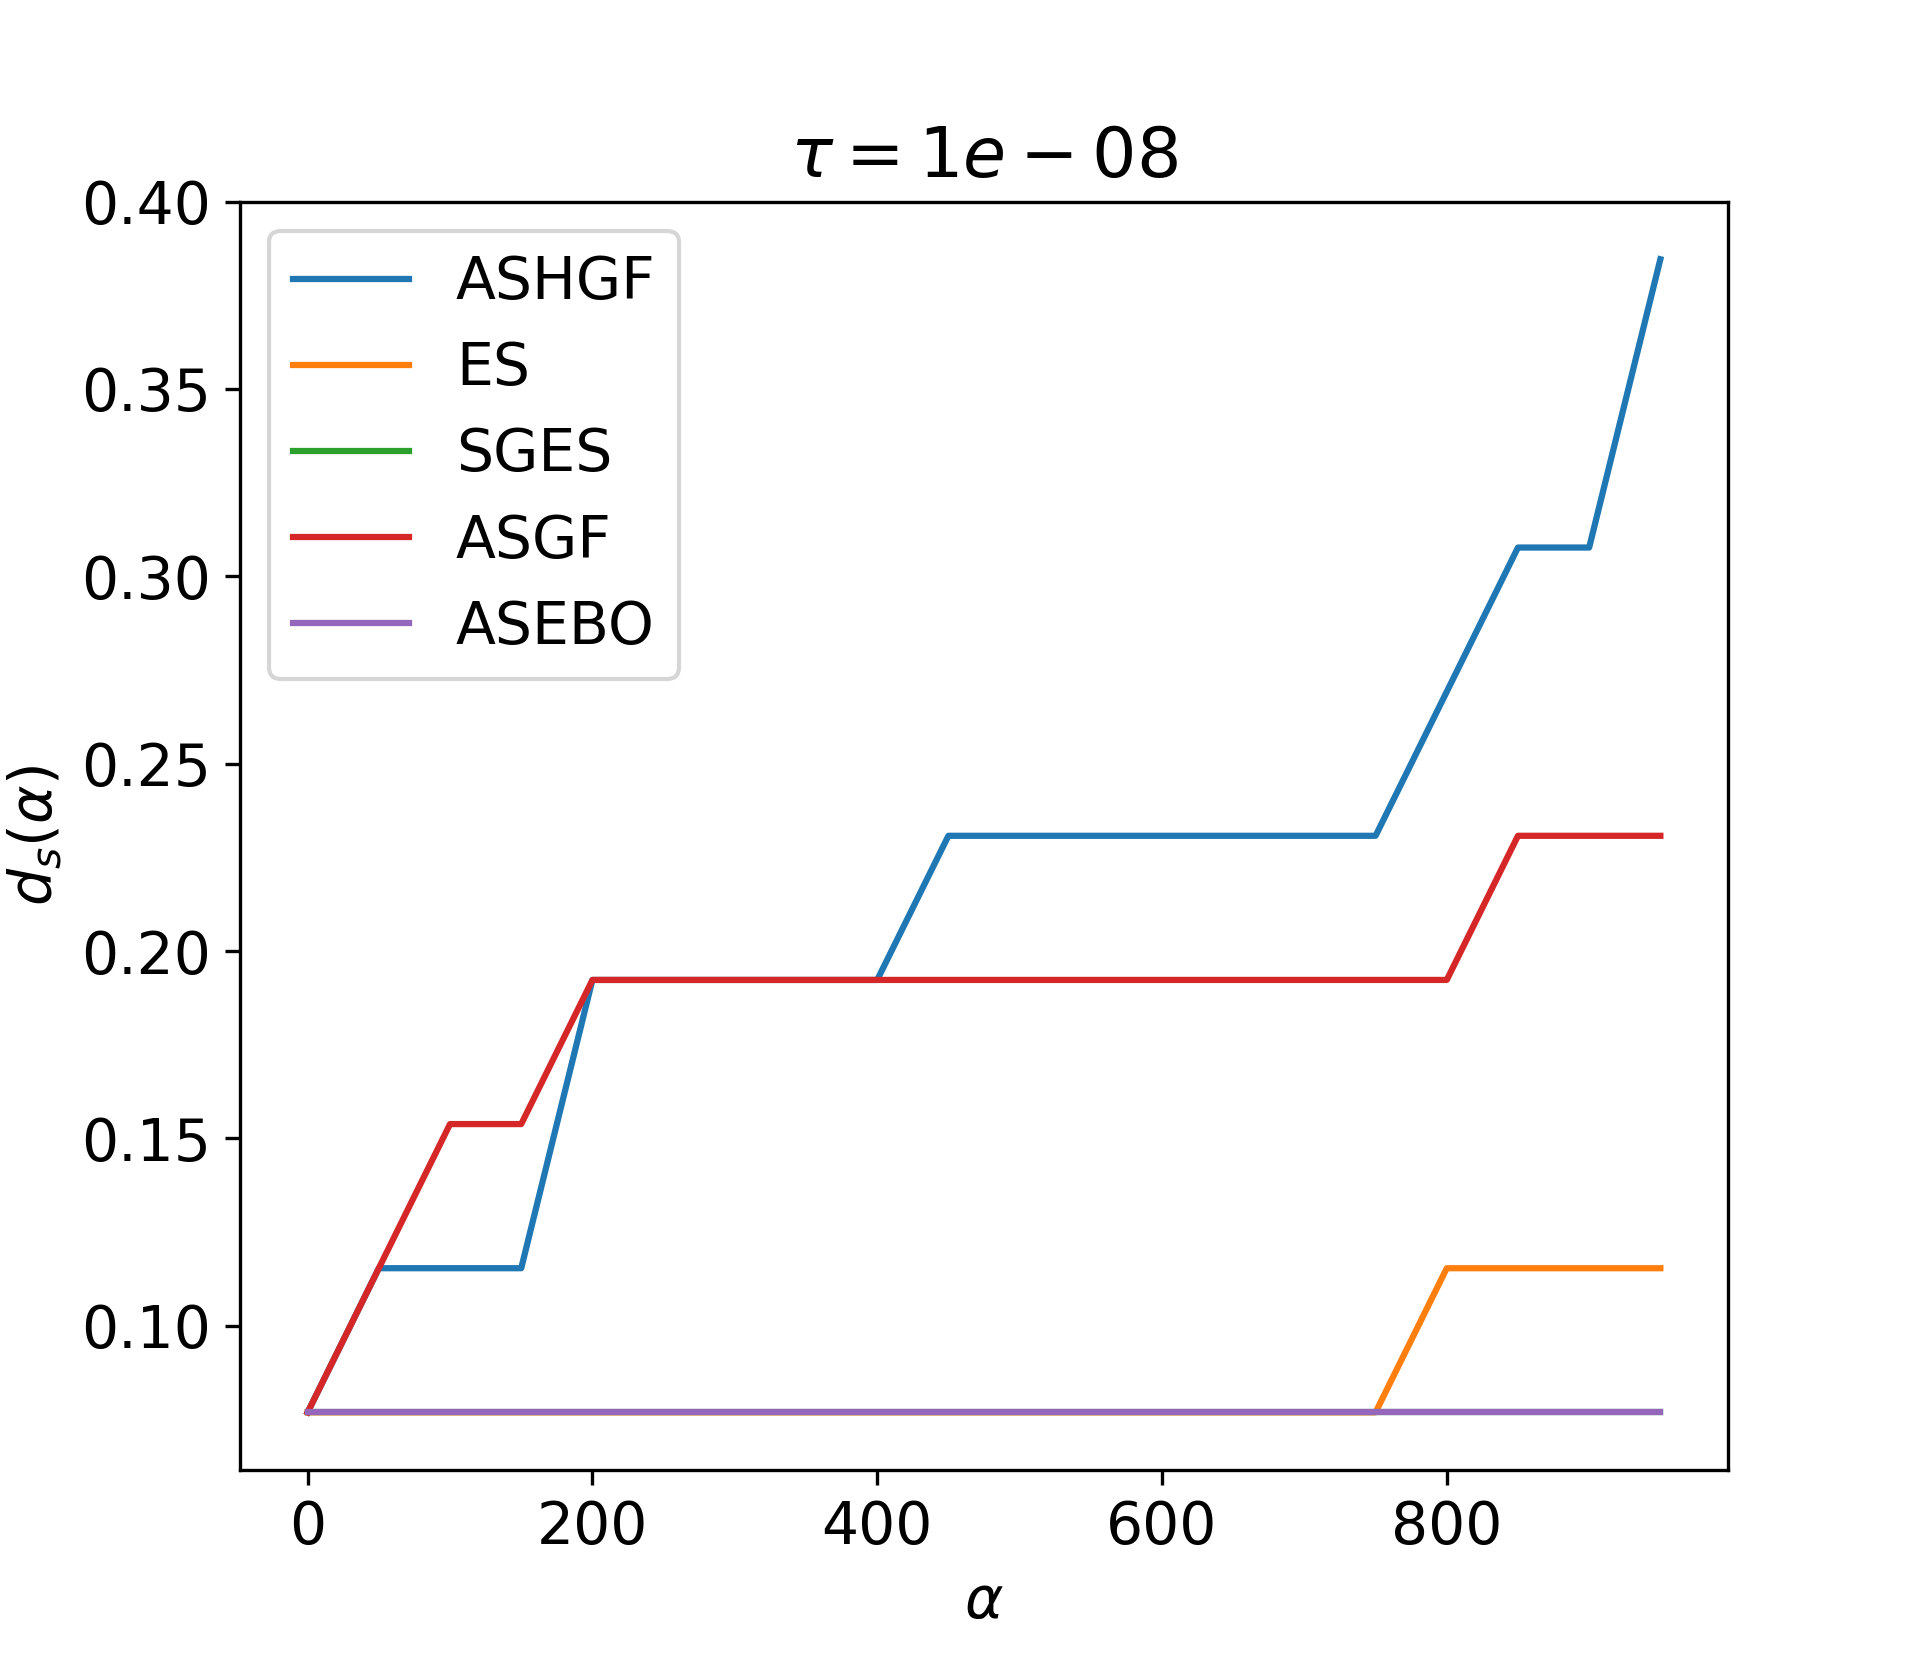
\includegraphics[width=1\textwidth]{figures/data_profiles/1000/data_profile_1000_1000000_1e-08.png}
\end{subfigure}%
\begin{subfigure}{0.3\textwidth}
  \centering 
  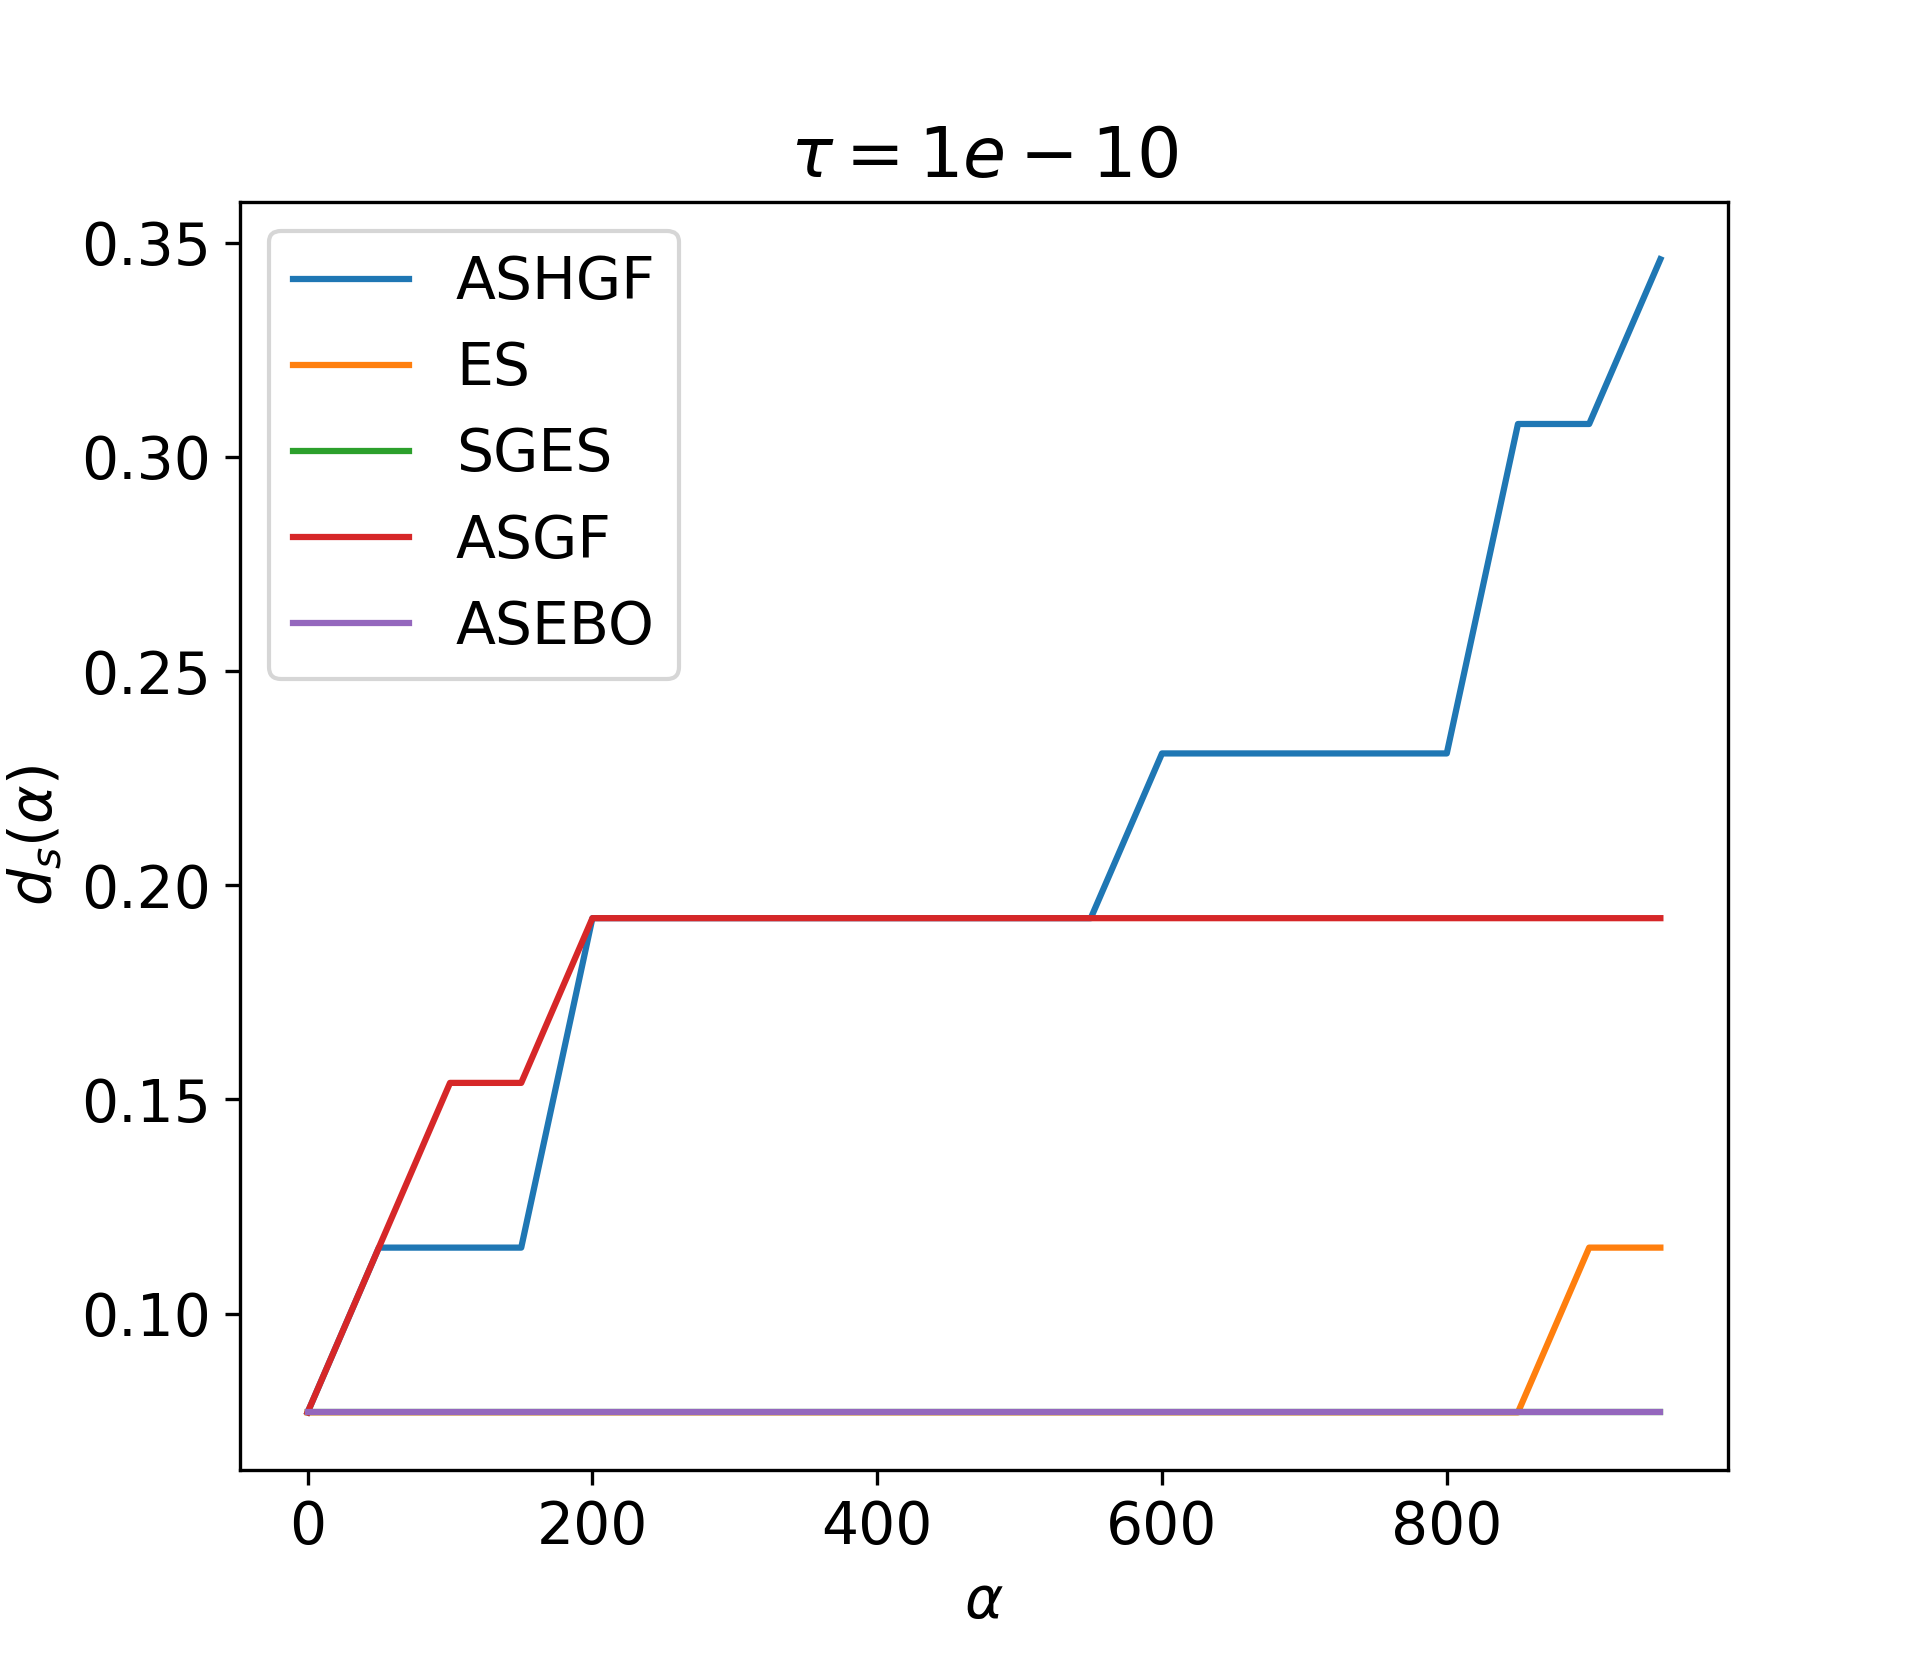
\includegraphics[width=1\textwidth]{figures/data_profiles/1000/data_profile_1000_1000000_1e-10.png}
\end{subfigure}
\caption{Data profiles with $\mu_L = 10^{6}$}
\label{DataProfiles1000Mu1000000}
\end{figure}

\begin{figure}[H]
\centering
\begin{subfigure}{0.3\textwidth}
  \centering 
  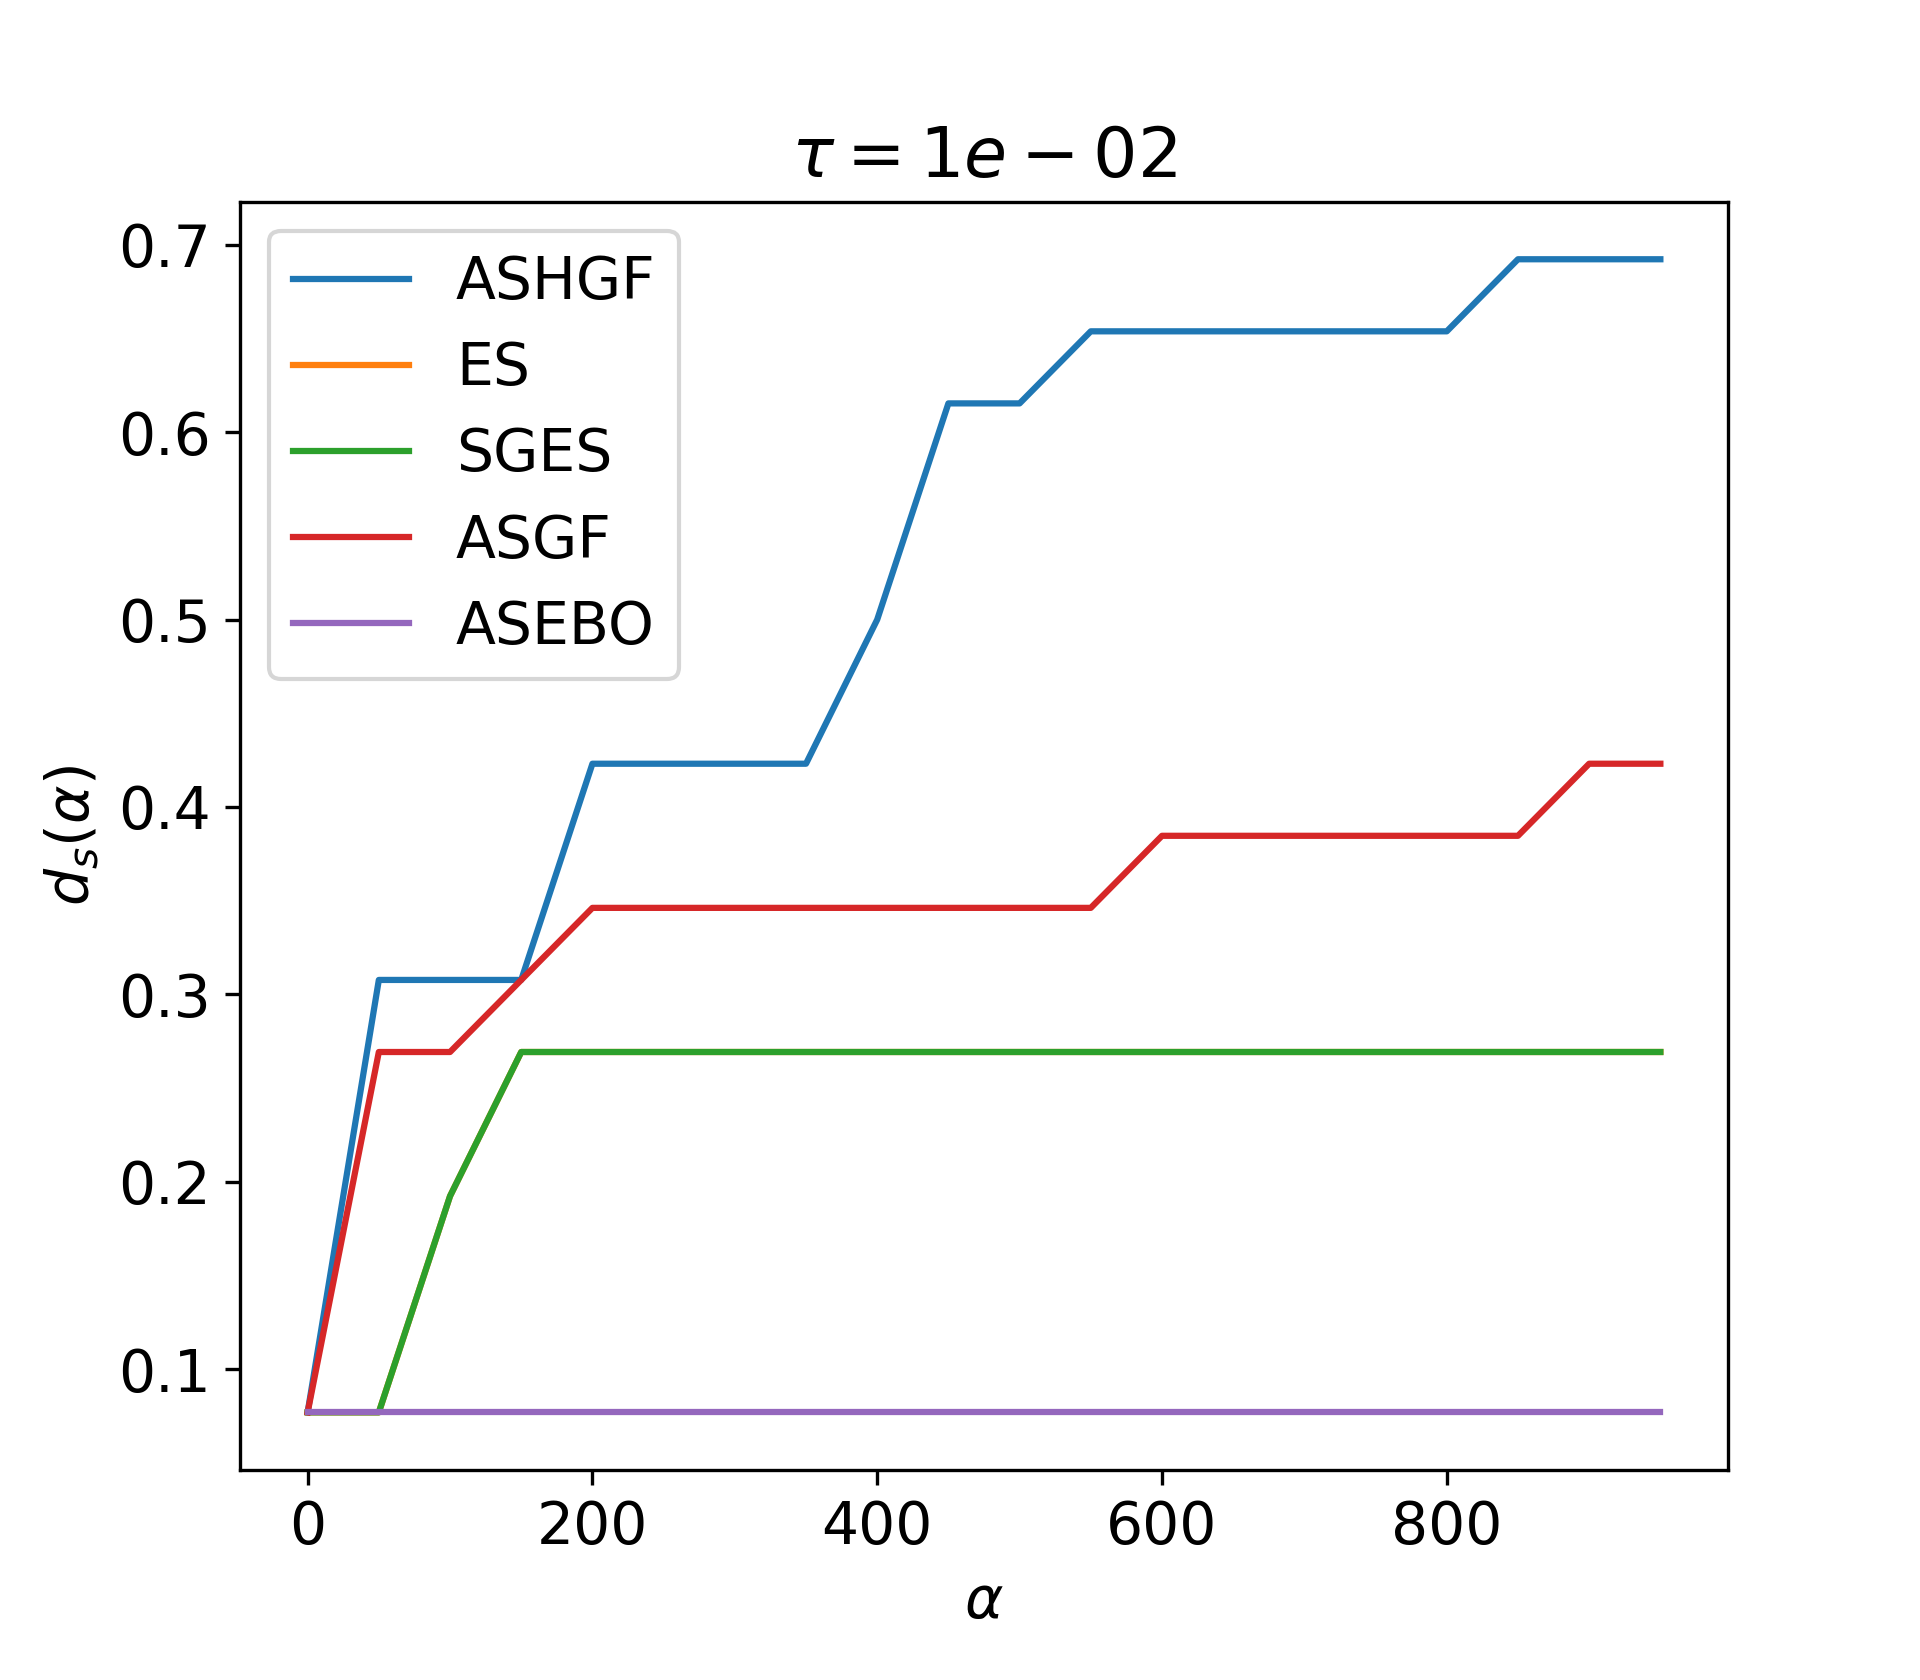
\includegraphics[width=1\textwidth]{figures/data_profiles/1000/data_profile_1000_10000000_1e-02.png}
\end{subfigure}%
\begin{subfigure}{0.3\textwidth}
  \centering 
  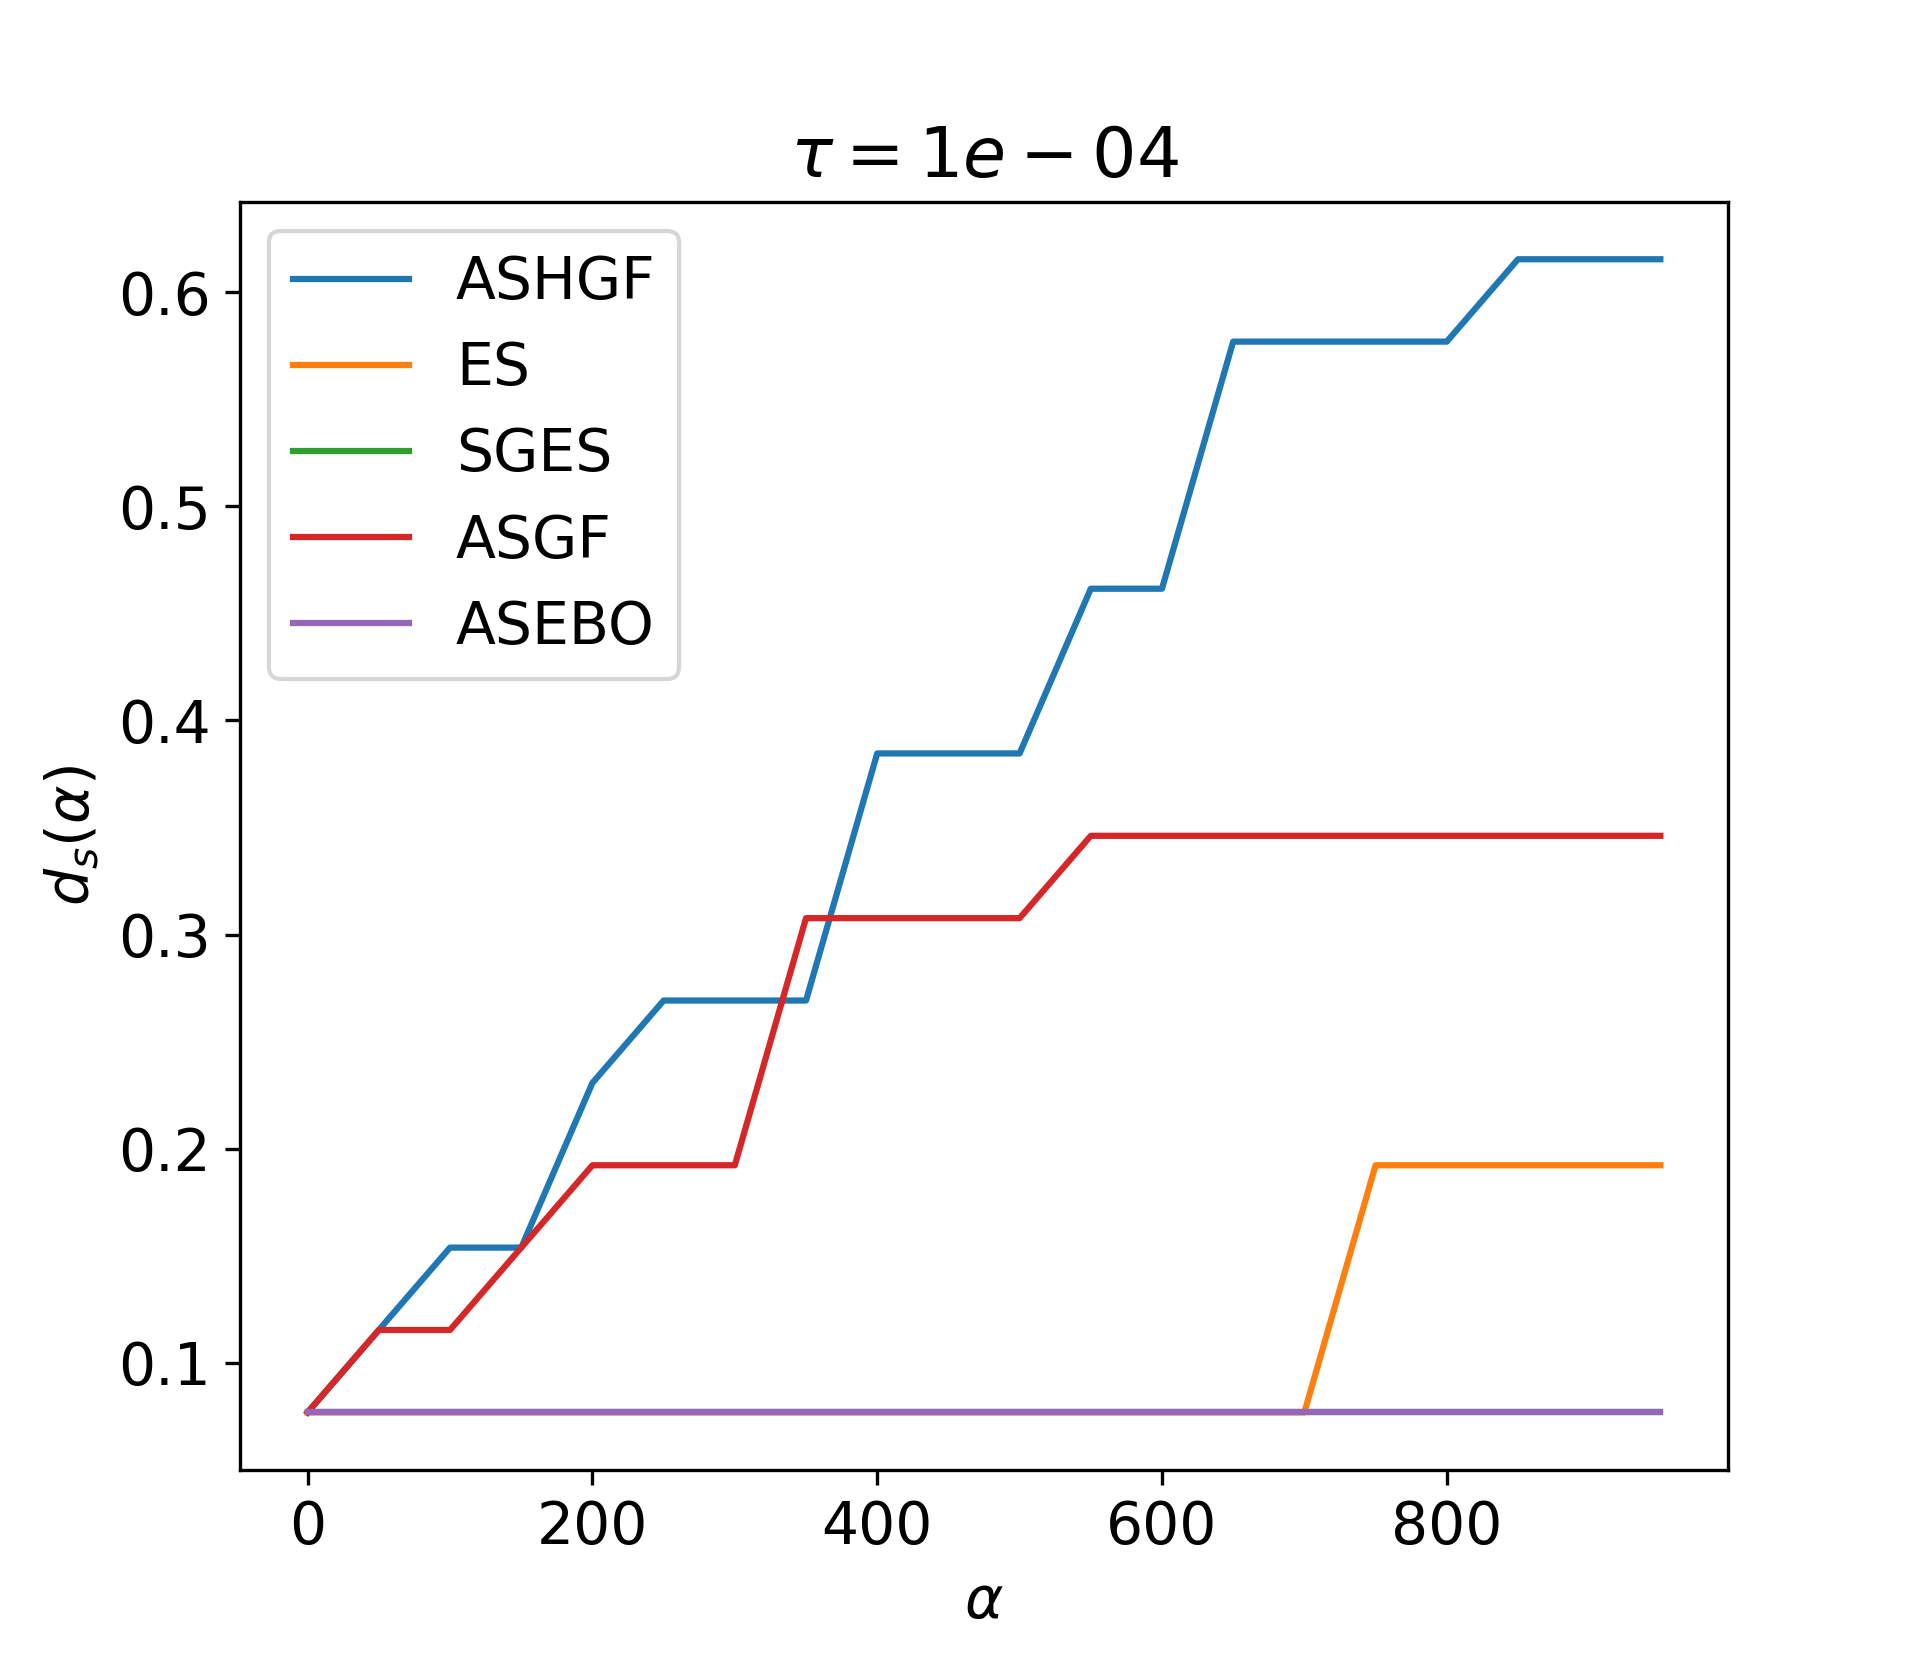
\includegraphics[width=1\textwidth]{figures/data_profiles/1000/data_profile_1000_10000000_1e-04.png}
\end{subfigure}
\begin{subfigure}{0.3\textwidth}
  \centering 
  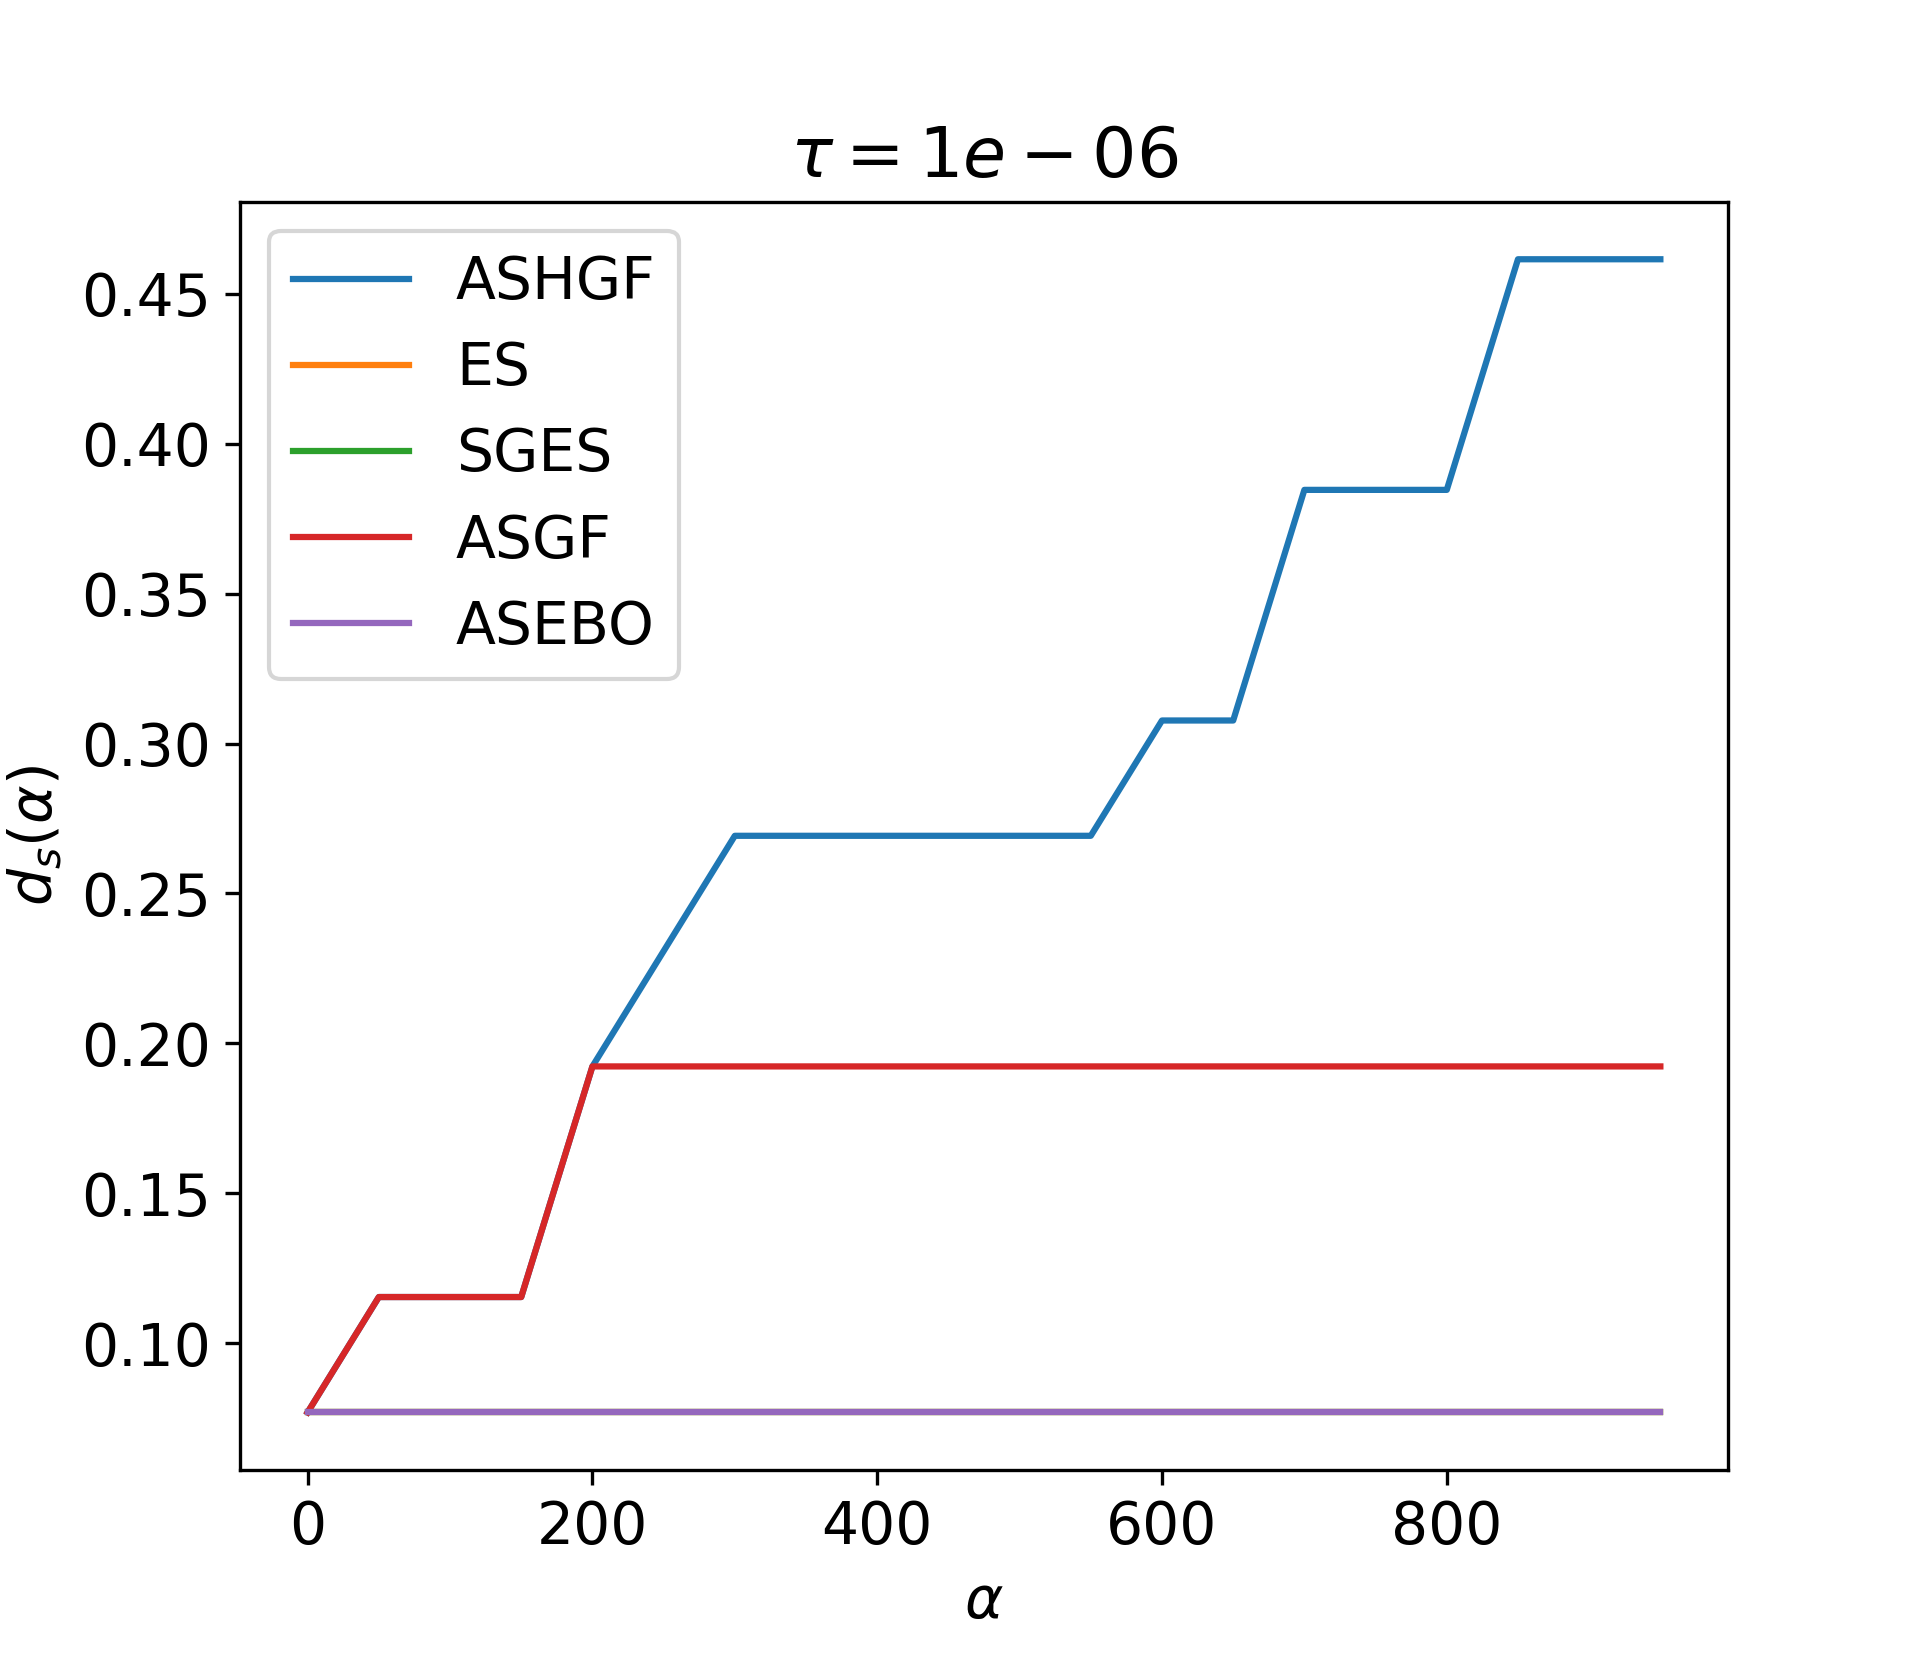
\includegraphics[width=1\textwidth]{figures/data_profiles/1000/data_profile_1000_10000000_1e-06.png}
\end{subfigure}
\centering
\begin{subfigure}{0.3\textwidth}
  \centering 
  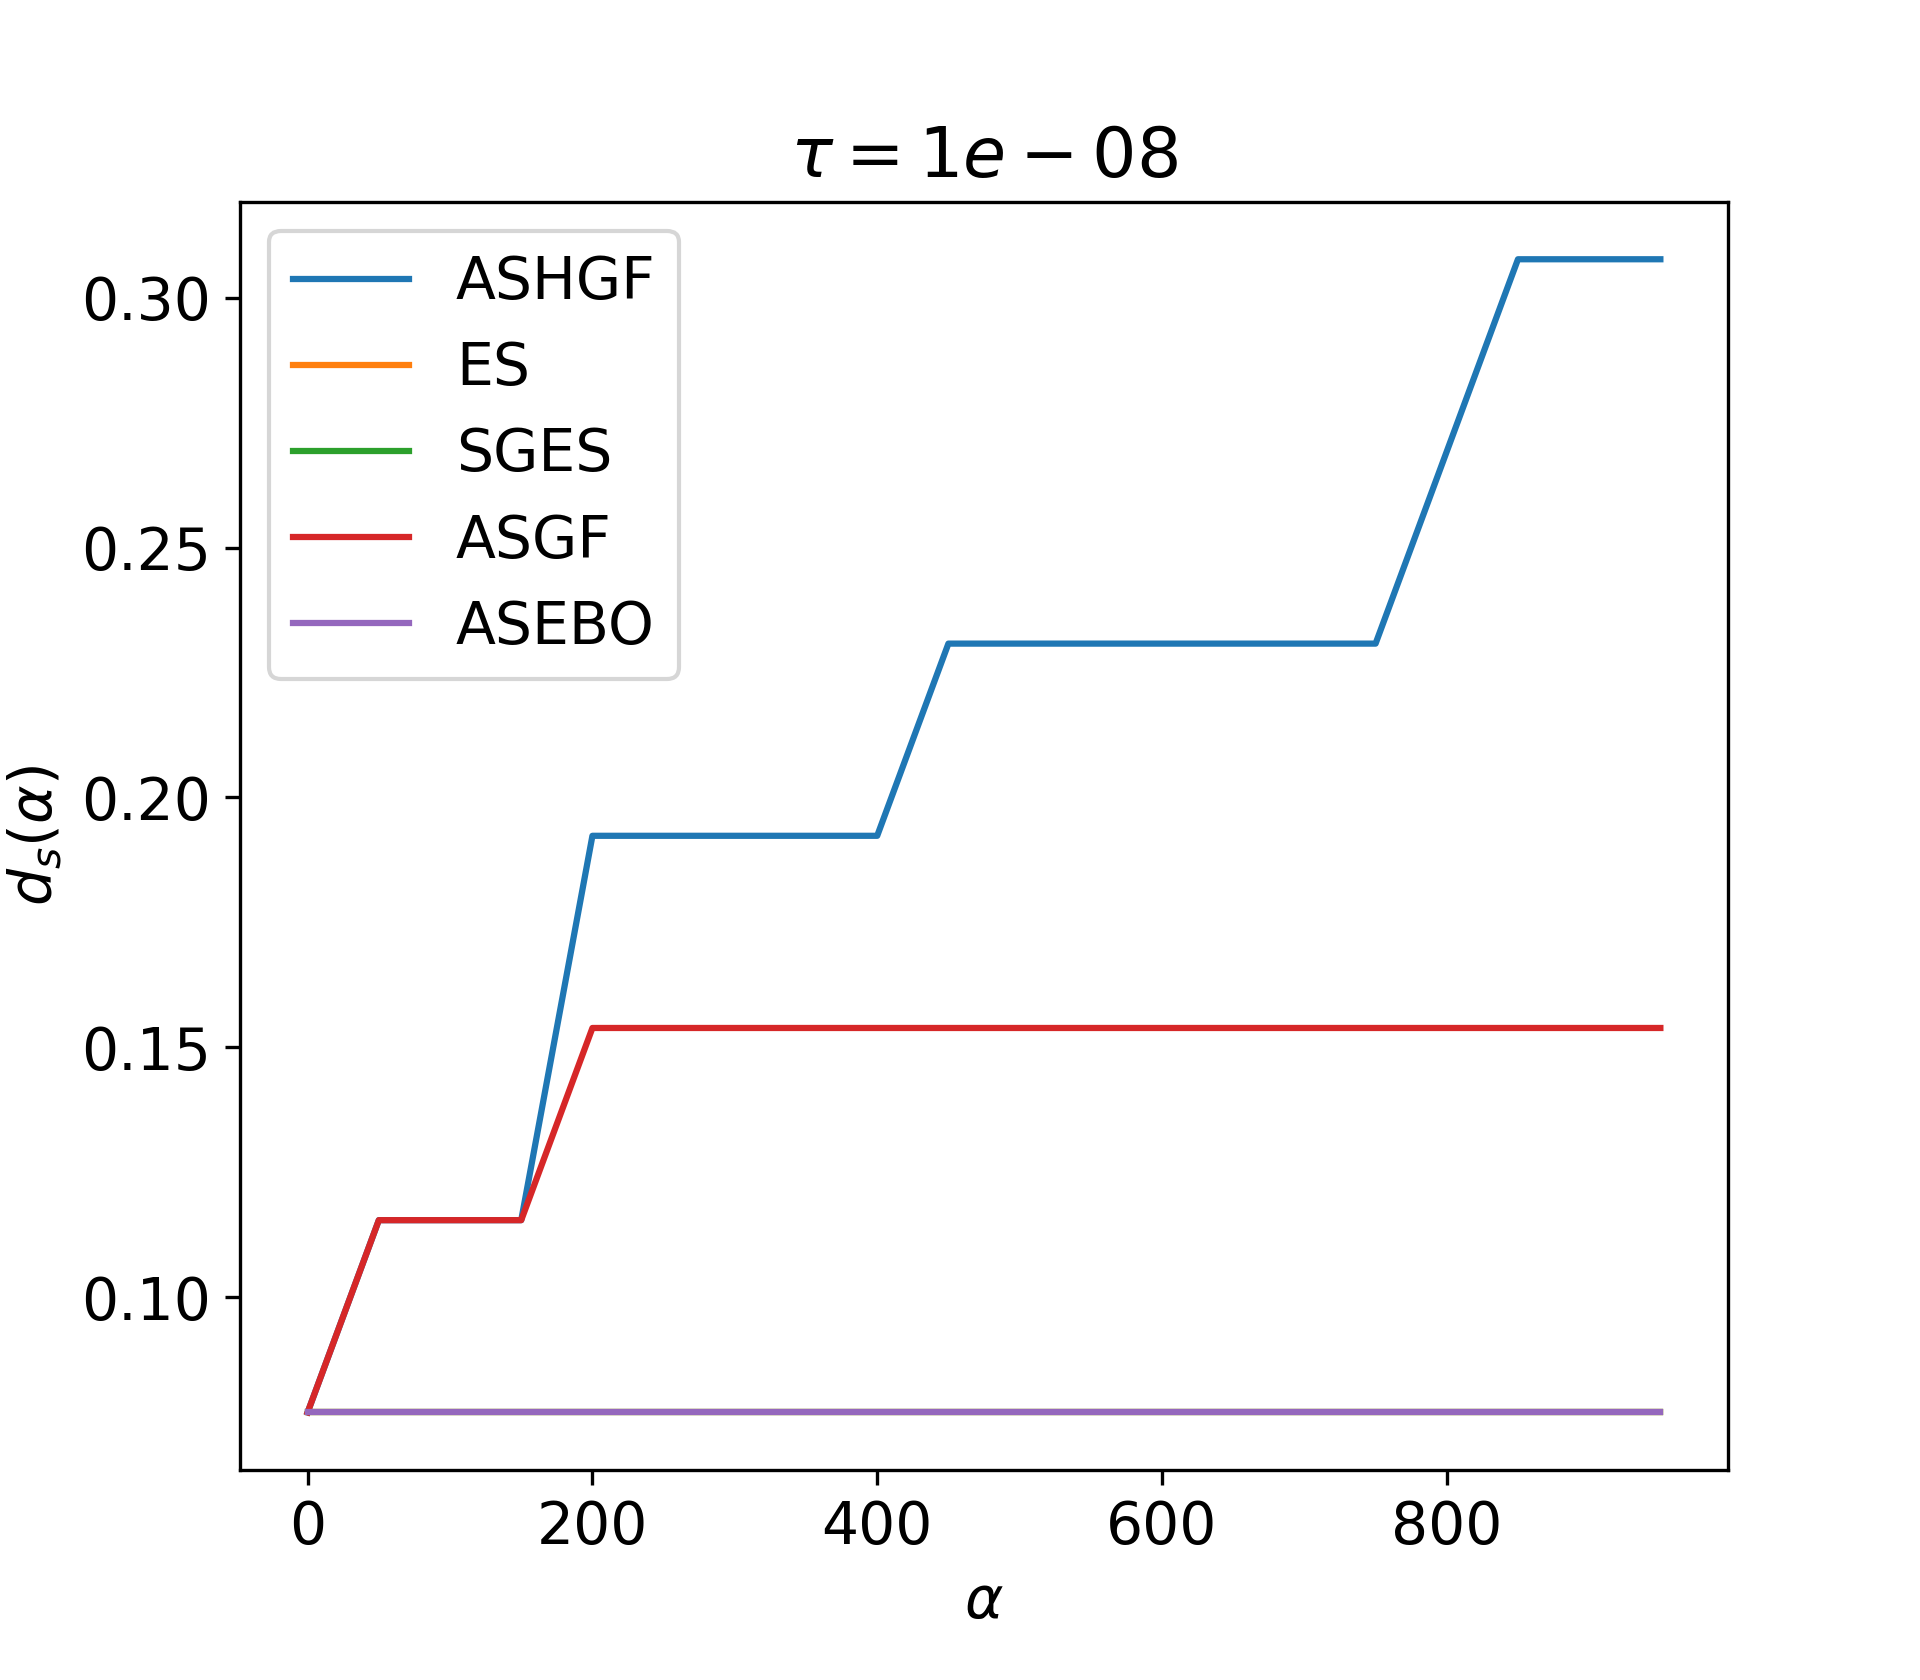
\includegraphics[width=1\textwidth]{figures/data_profiles/1000/data_profile_1000_10000000_1e-08.png}
\end{subfigure}%
\begin{subfigure}{0.3\textwidth}
  \centering 
  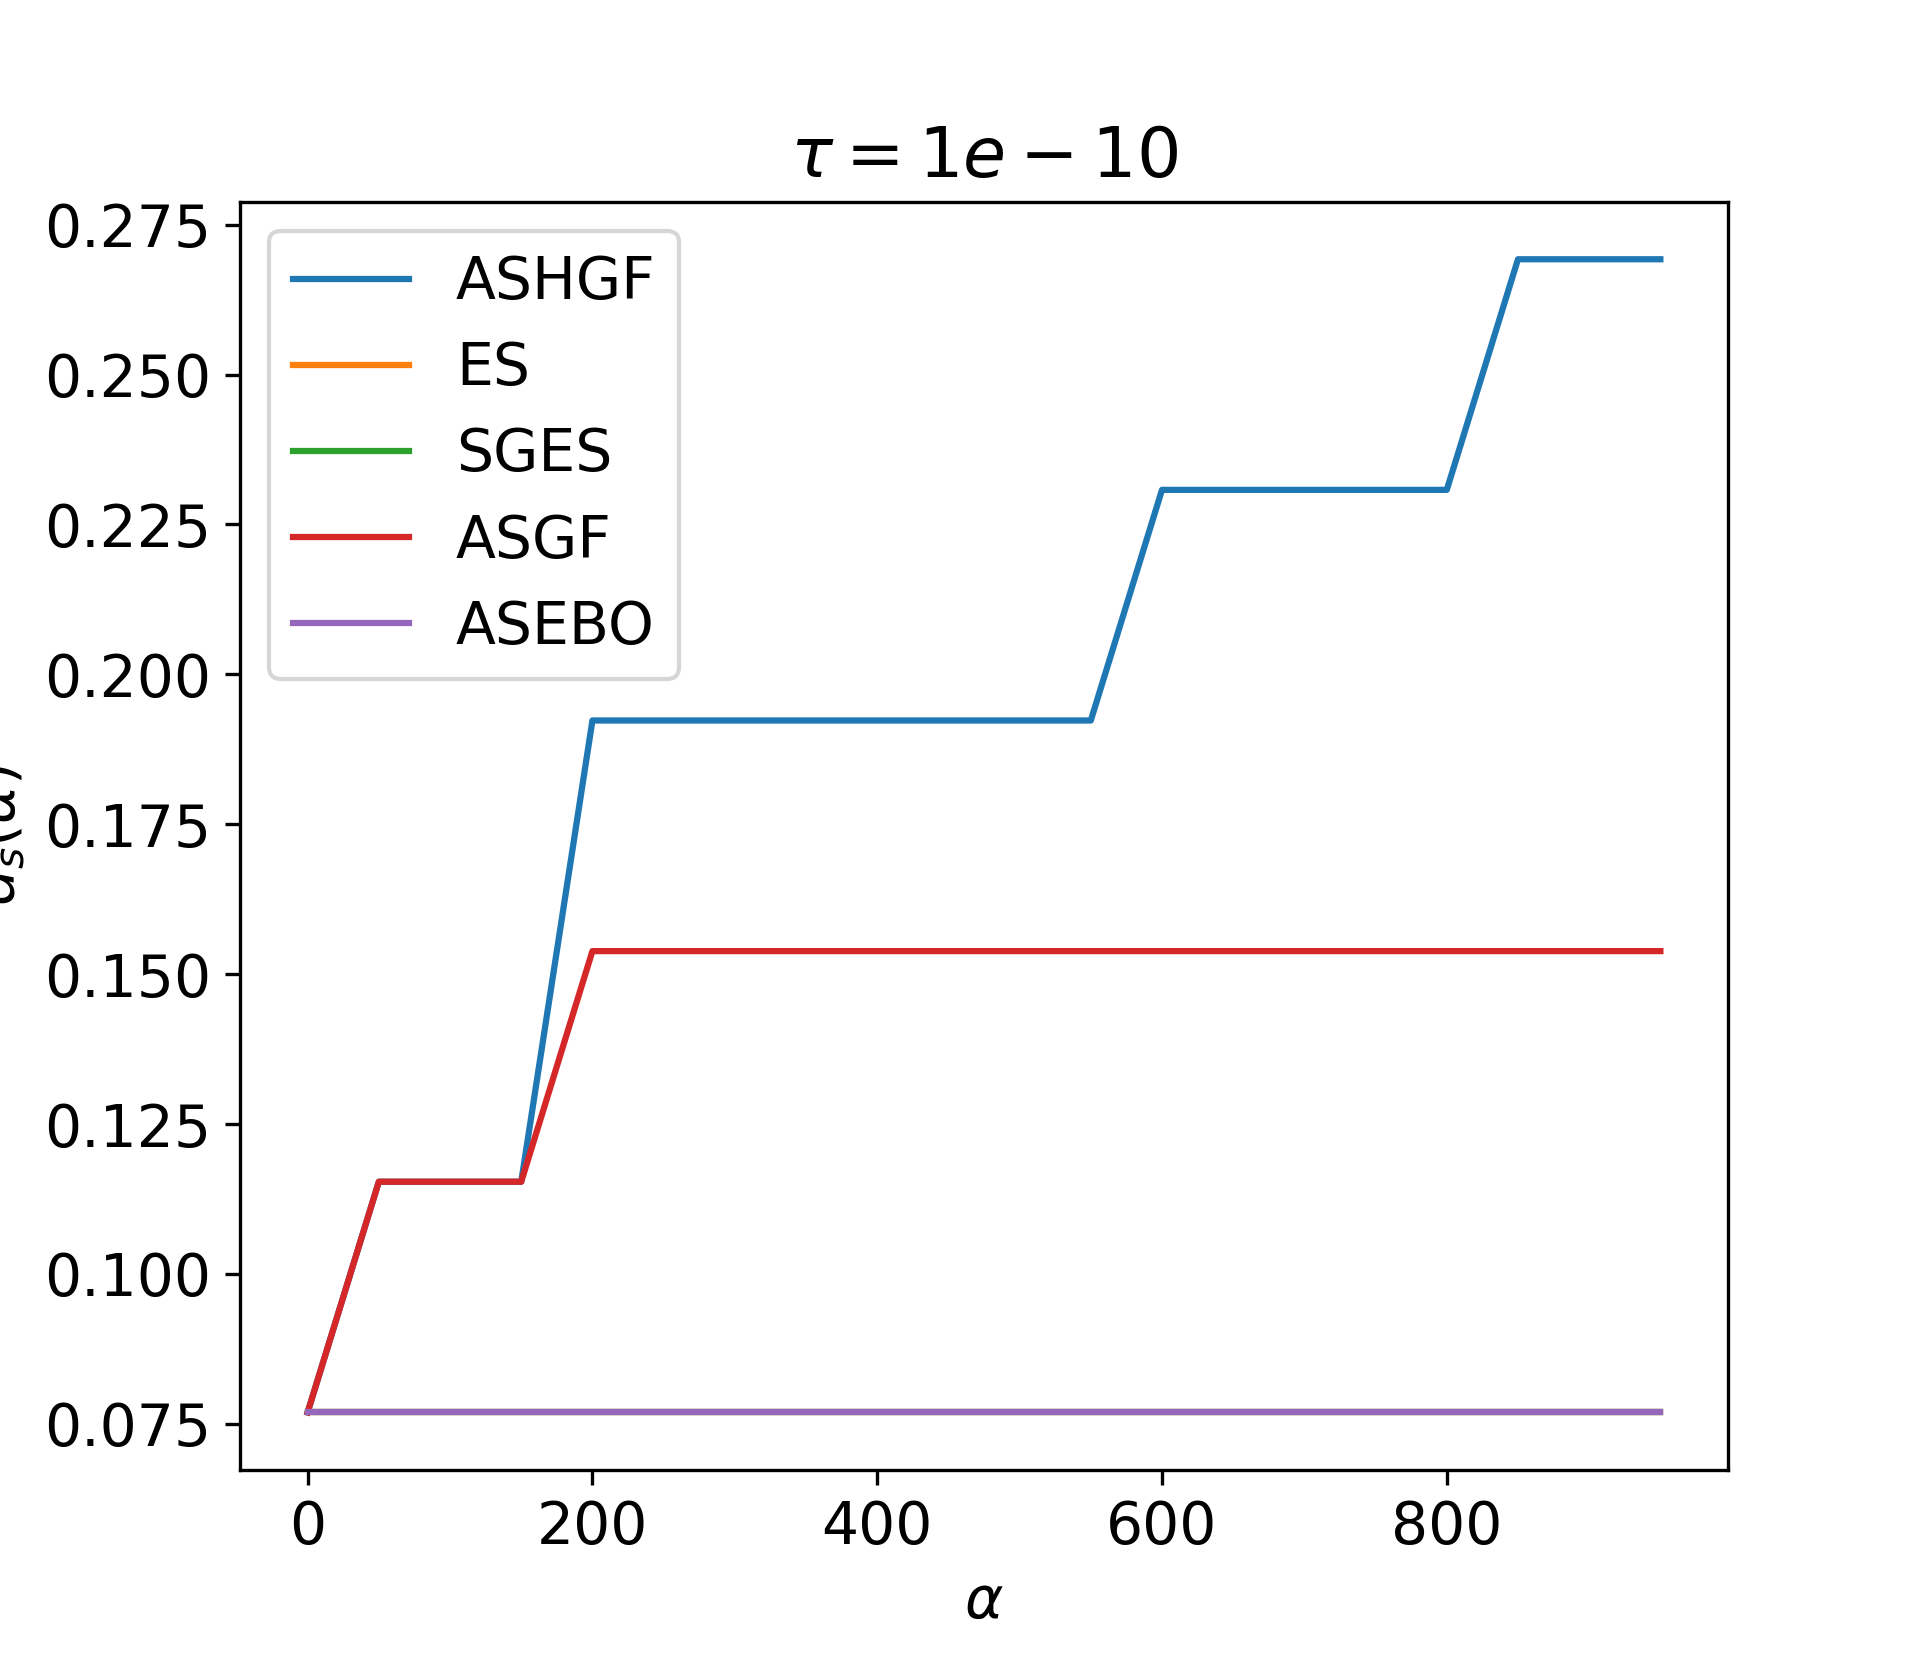
\includegraphics[width=1\textwidth]{figures/data_profiles/1000/data_profile_1000_10000000_1e-10.png}
\end{subfigure}
\caption{Data profiles with $\mu_L = 10^{7}$}
\label{DataProfiles1000Mu10000000}
\end{figure}

\begin{figure}[H]
	\centering
	\begin{subfigure}{0.3\textwidth}
		\centering 
		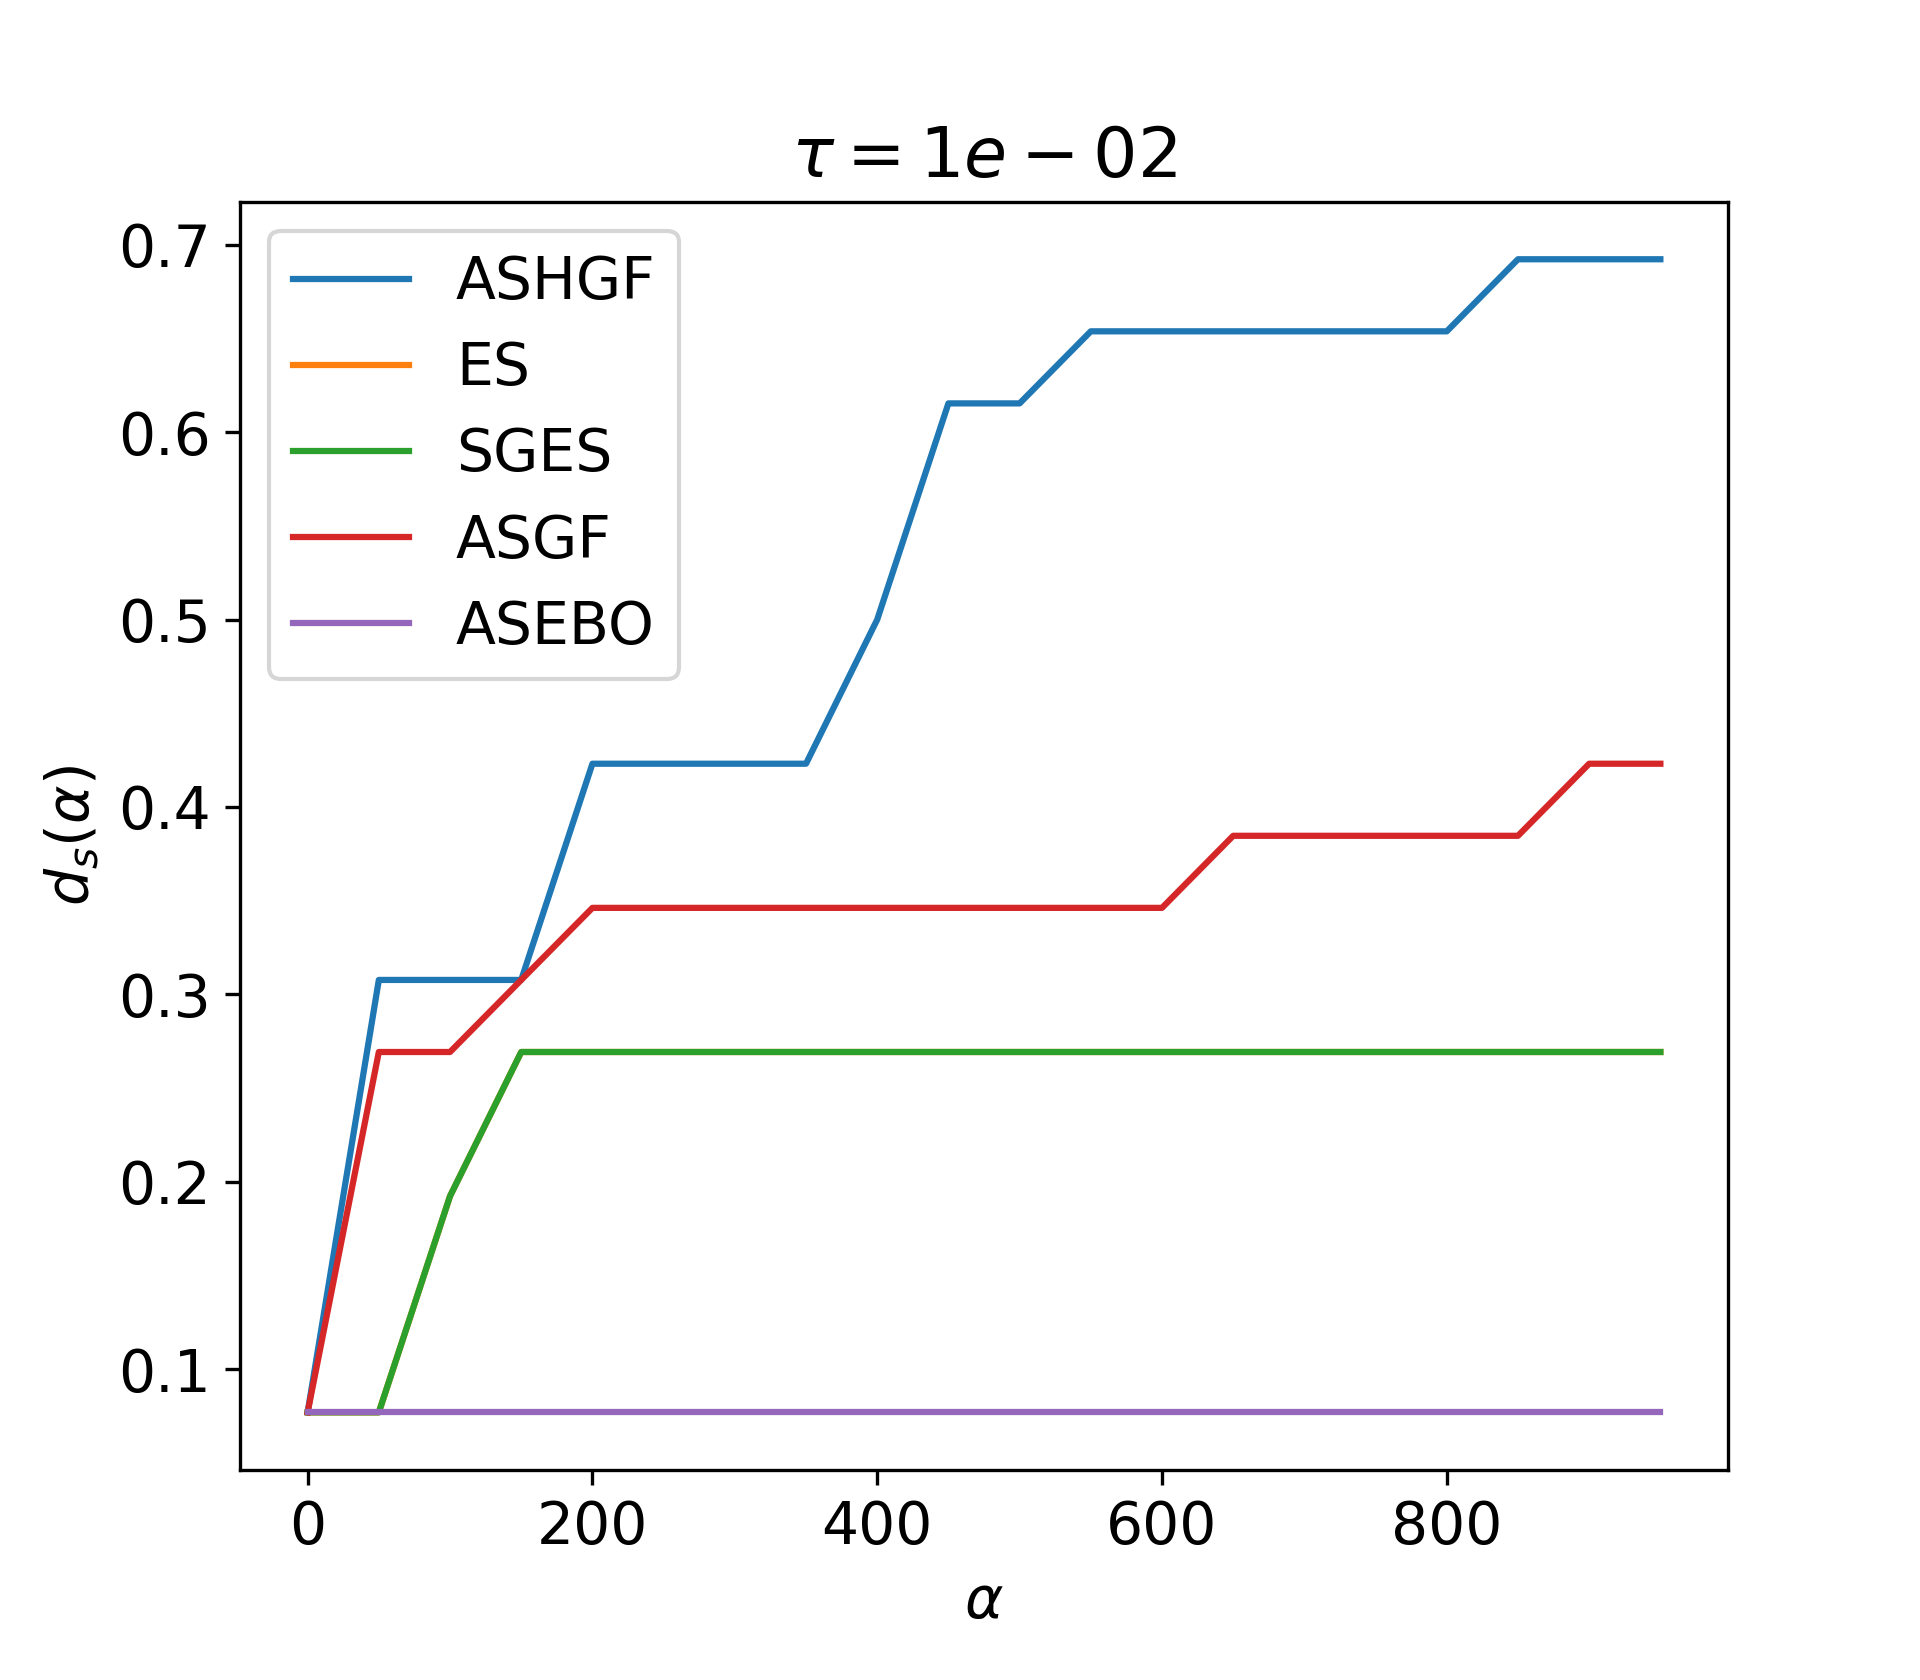
\includegraphics[width=1\textwidth]{figures/data_profiles/1000/data_profile_1000_100000000_1e-02.png}
	\end{subfigure}%
	\begin{subfigure}{0.3\textwidth}
		\centering 
		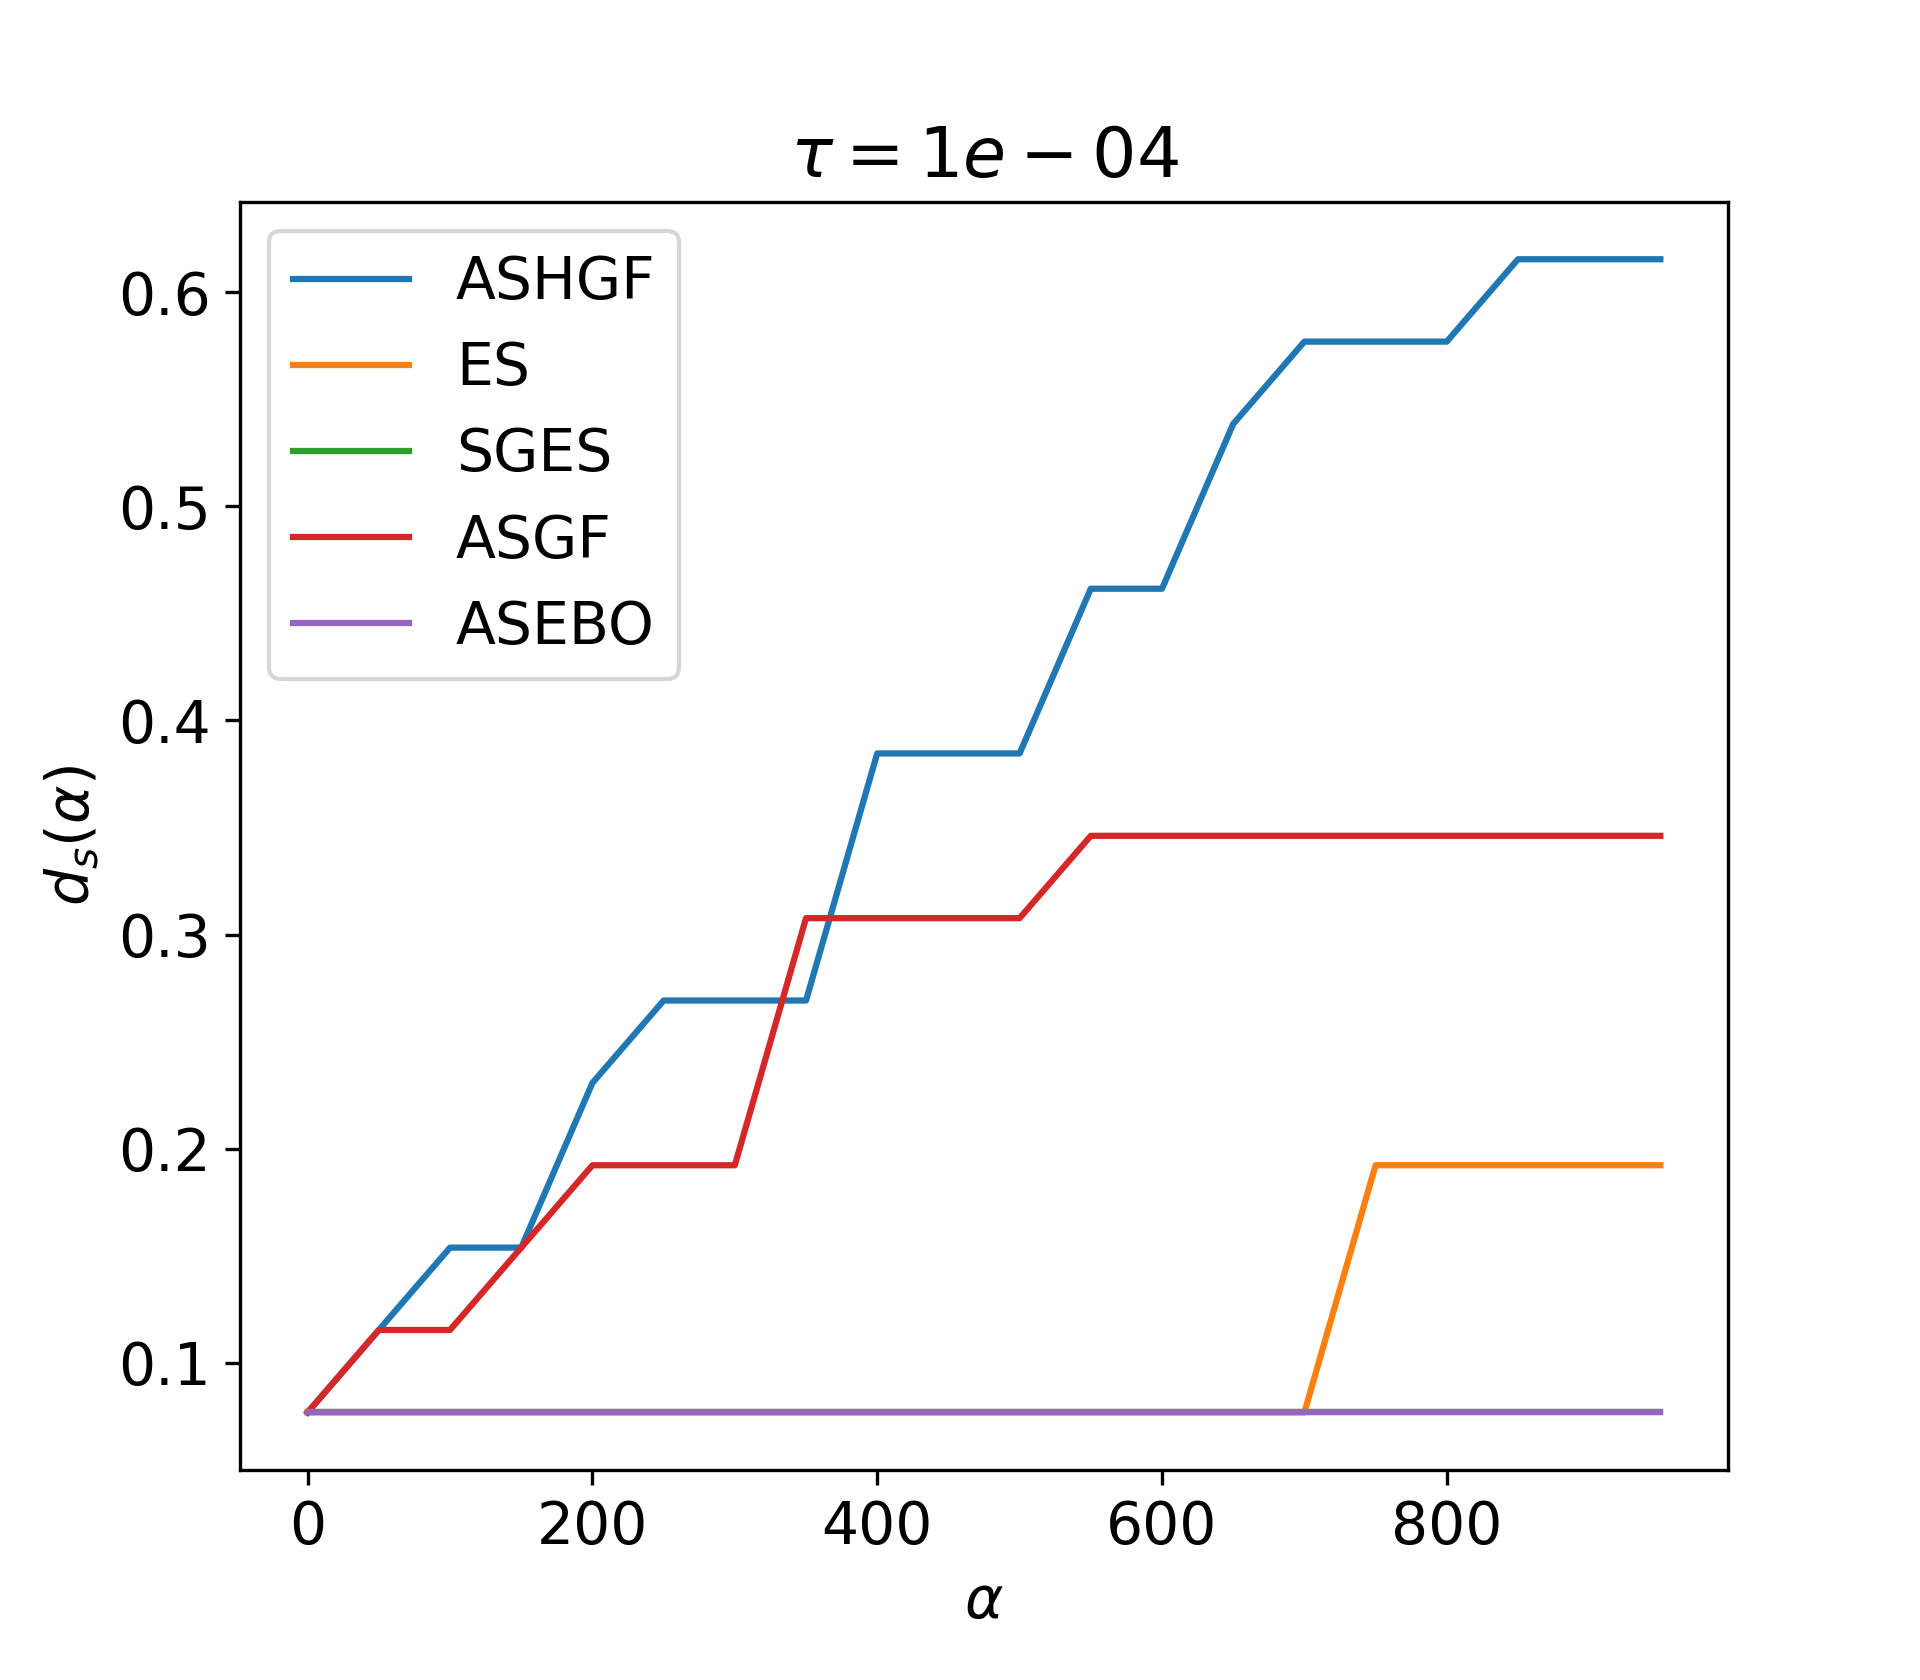
\includegraphics[width=1\textwidth]{figures/data_profiles/1000/data_profile_1000_100000000_1e-04.png}
	\end{subfigure}
	\begin{subfigure}{0.3\textwidth}
		\centering 
		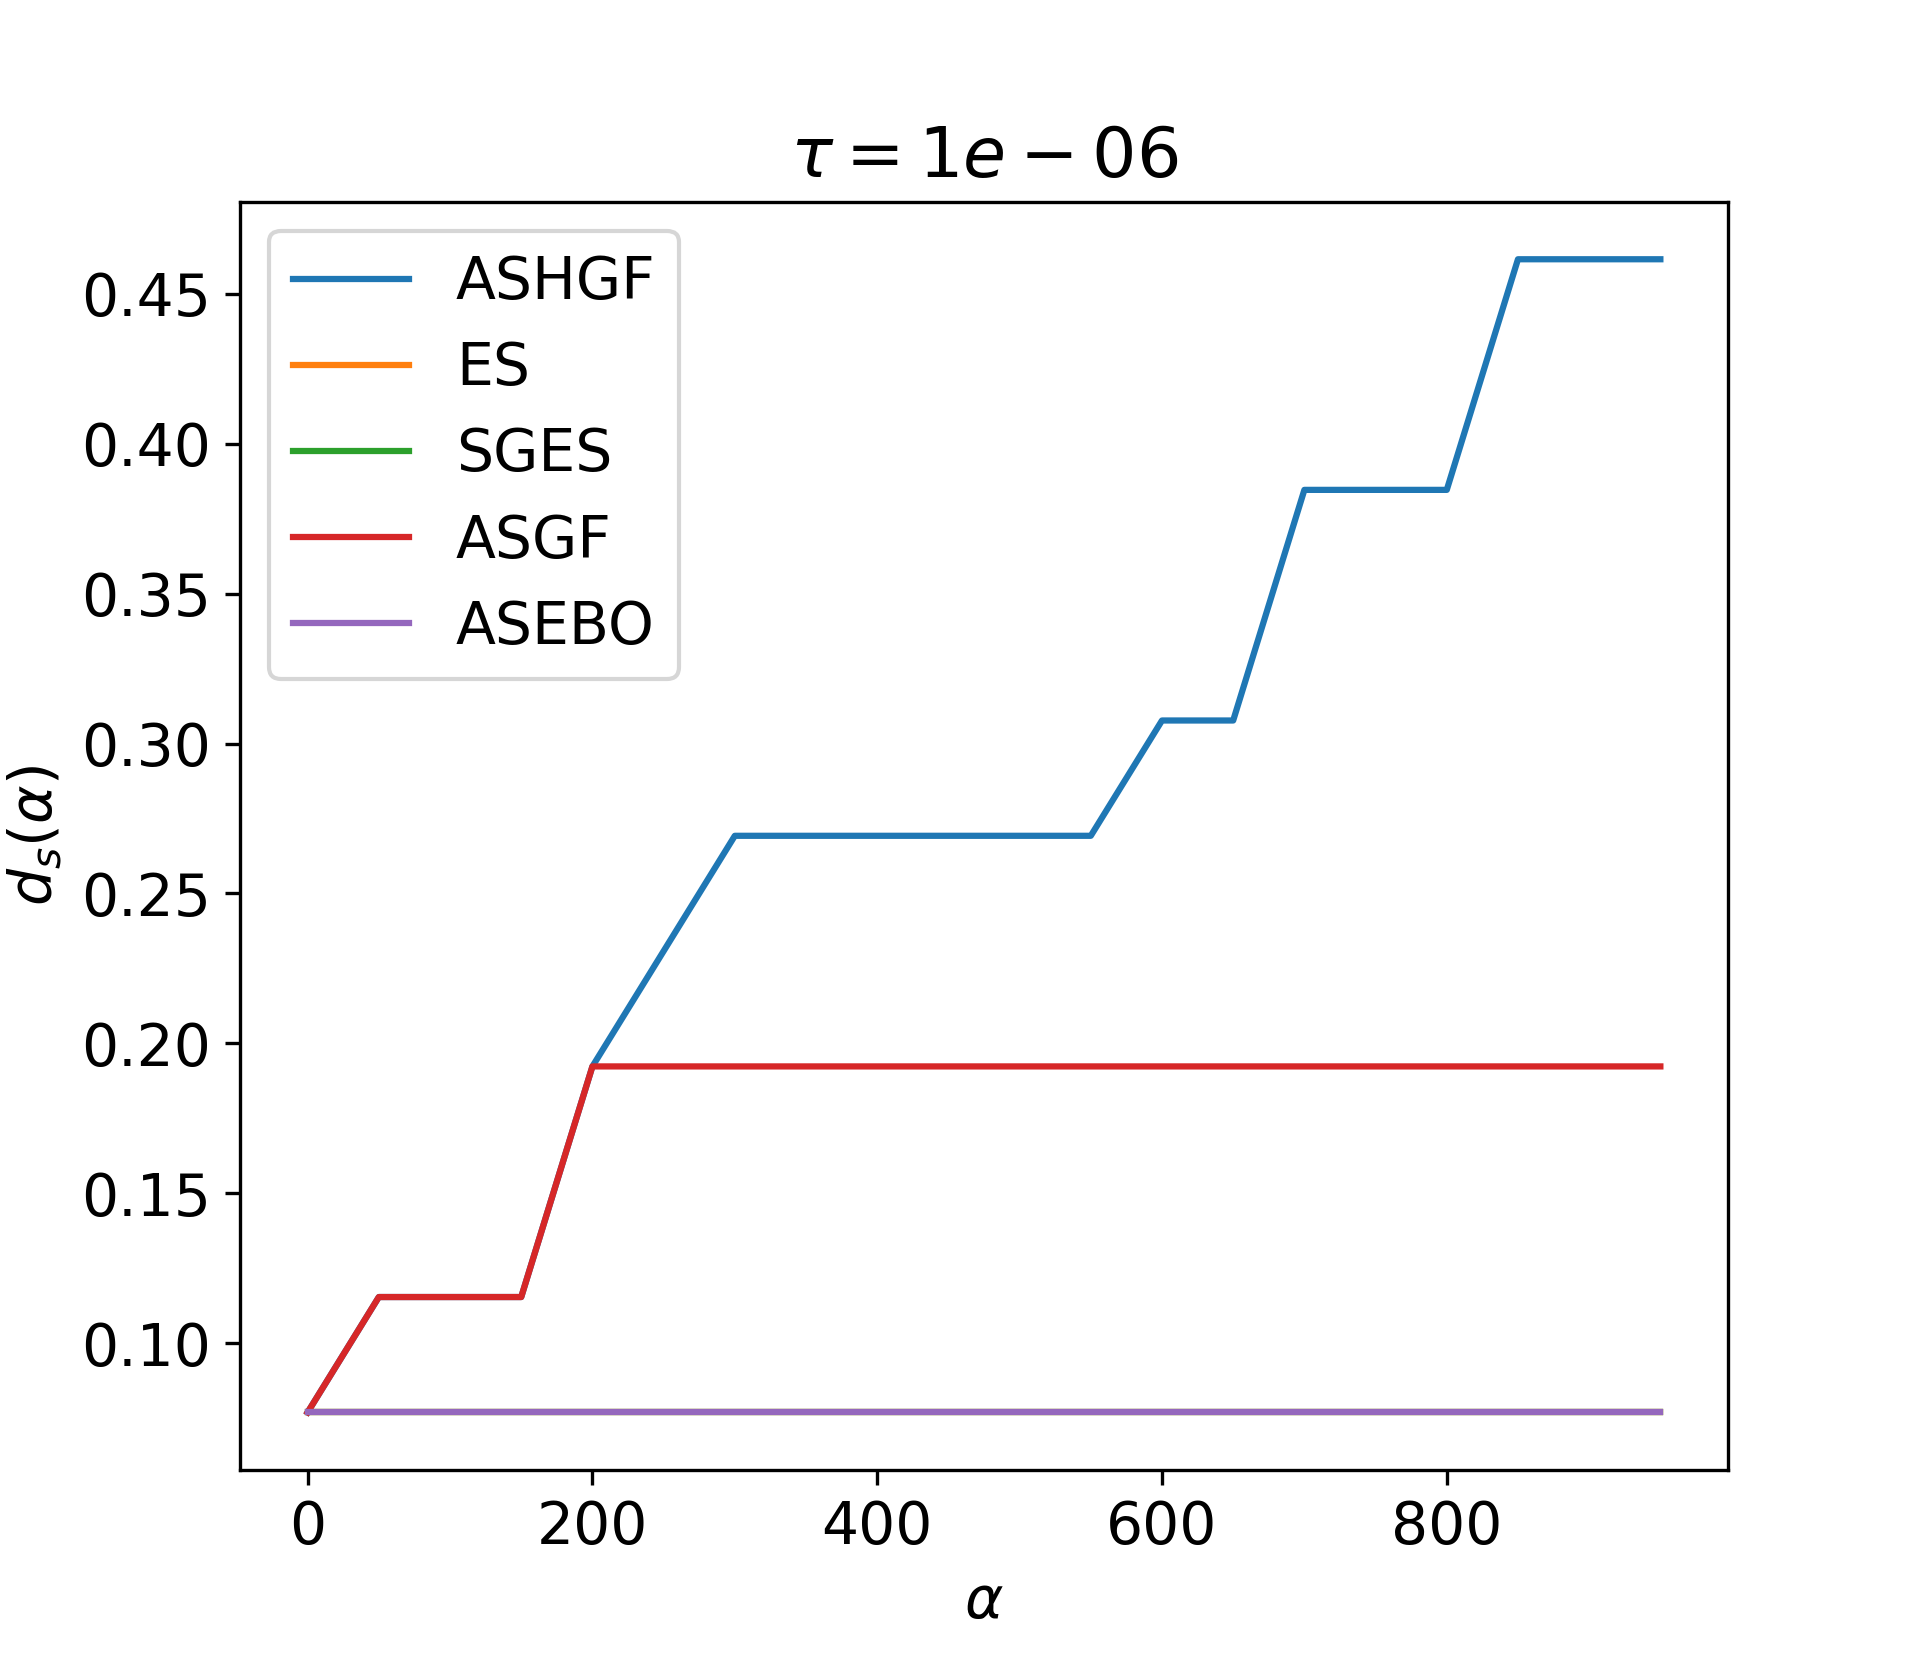
\includegraphics[width=1\textwidth]{figures/data_profiles/1000/data_profile_1000_100000000_1e-06.png}
	\end{subfigure}
	\centering
	\begin{subfigure}{0.3\textwidth}
		\centering 
		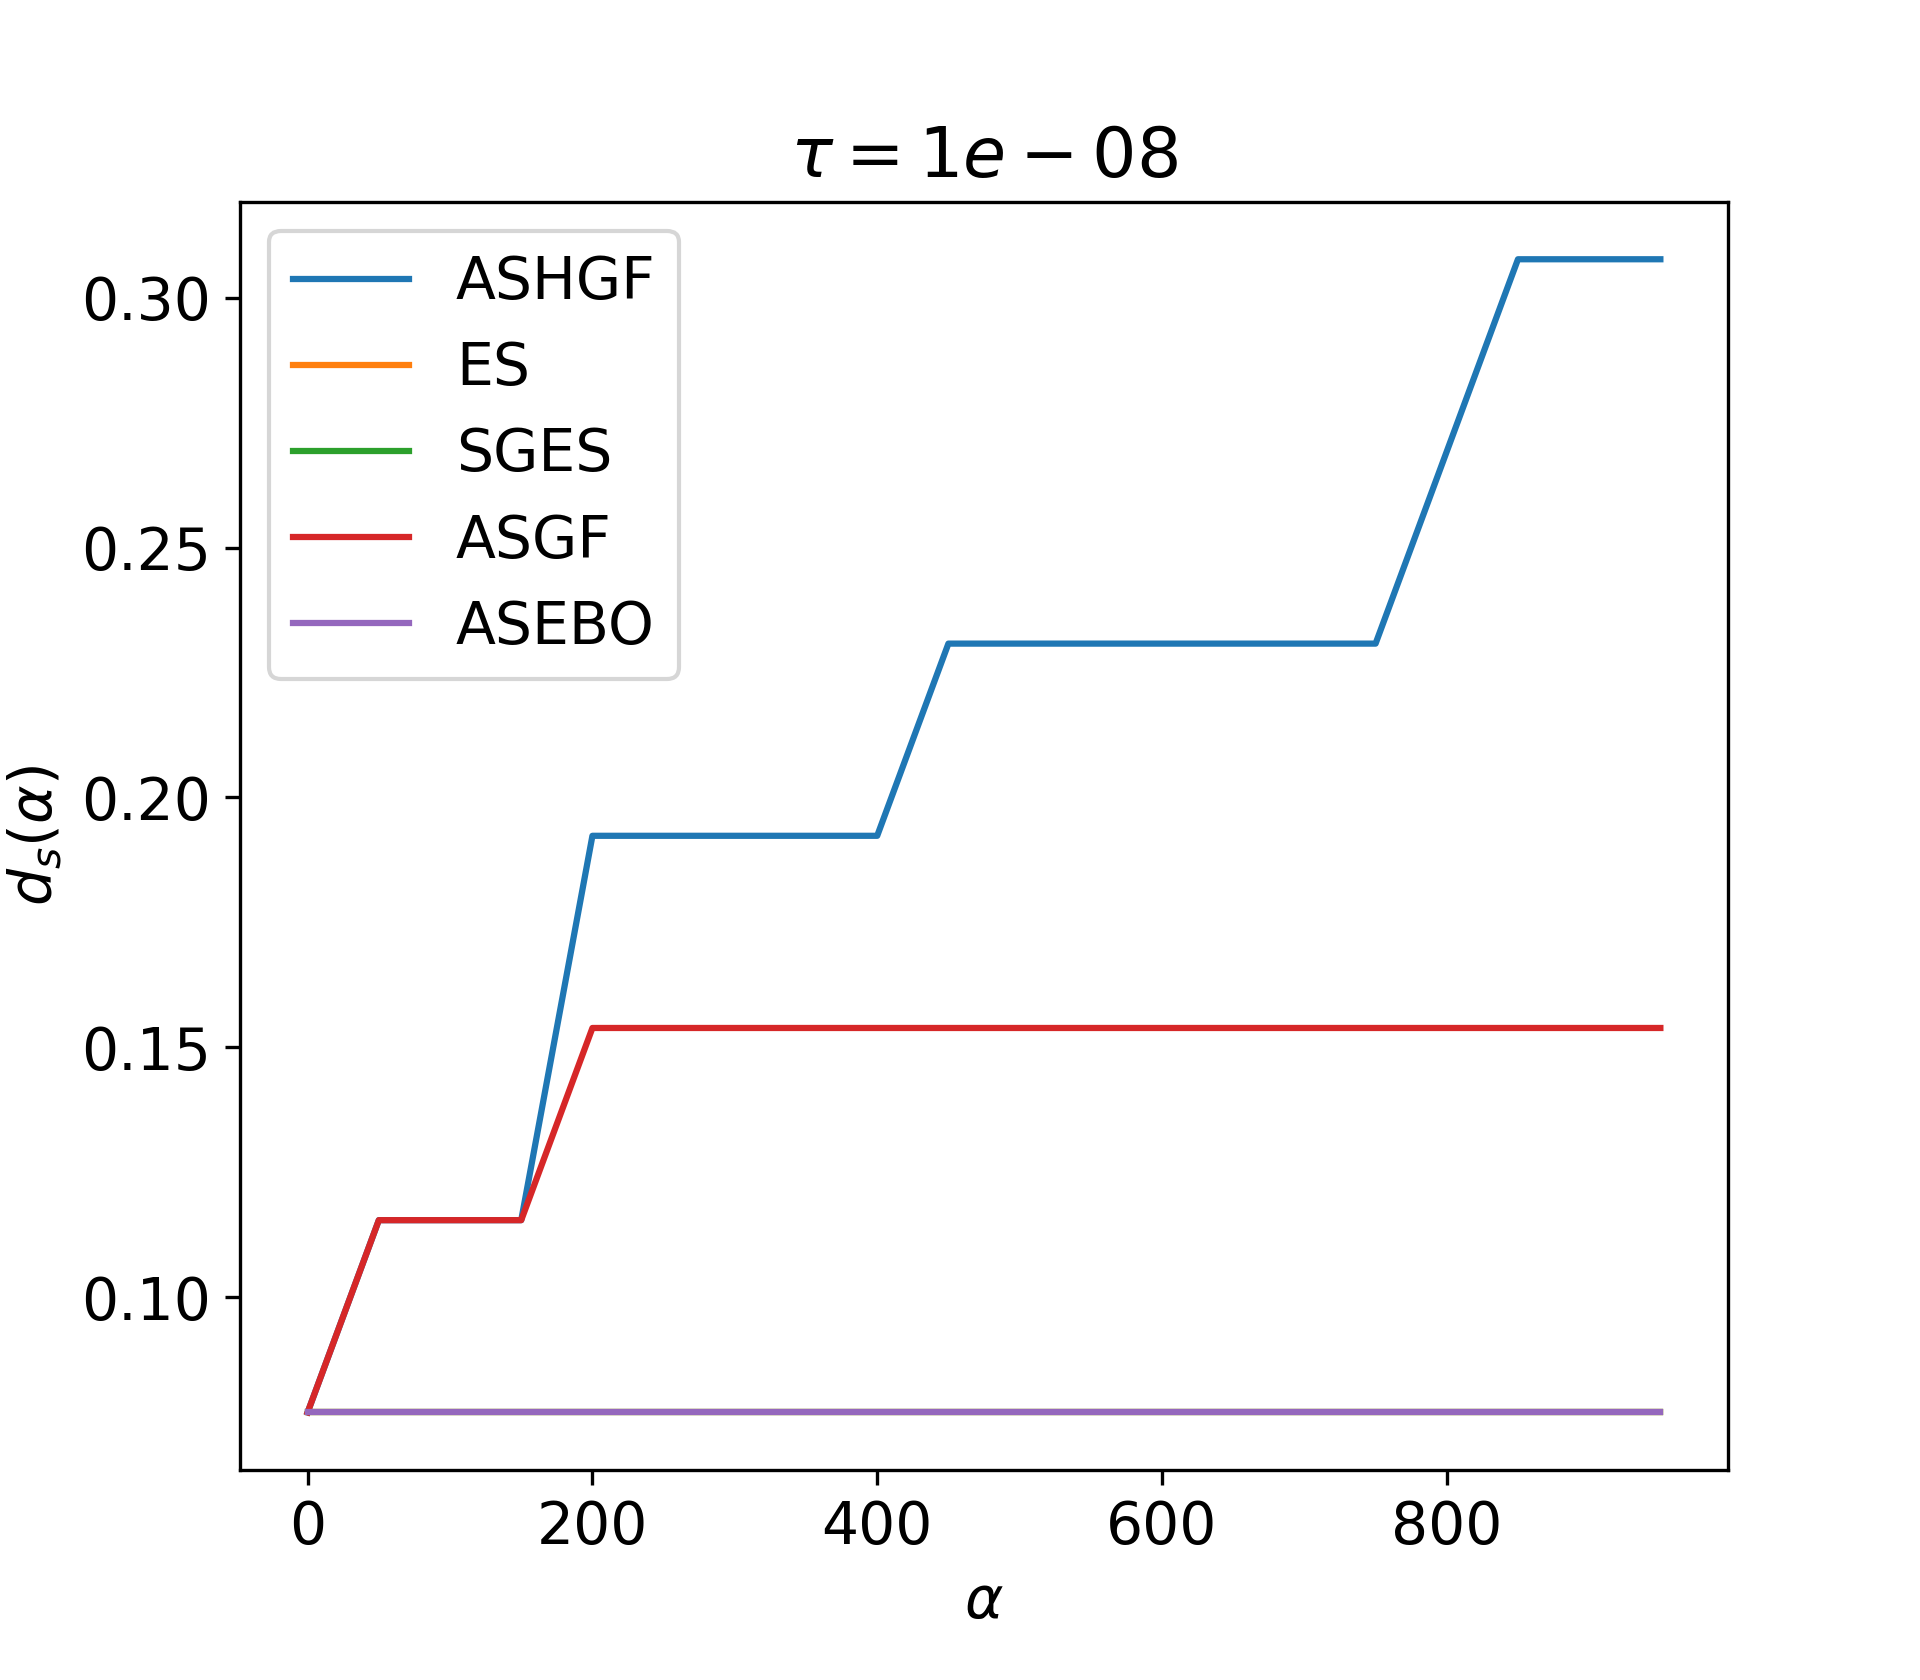
\includegraphics[width=1\textwidth]{figures/data_profiles/1000/data_profile_1000_100000000_1e-08.png}
	\end{subfigure}%
	\begin{subfigure}{0.3\textwidth}
		\centering 
		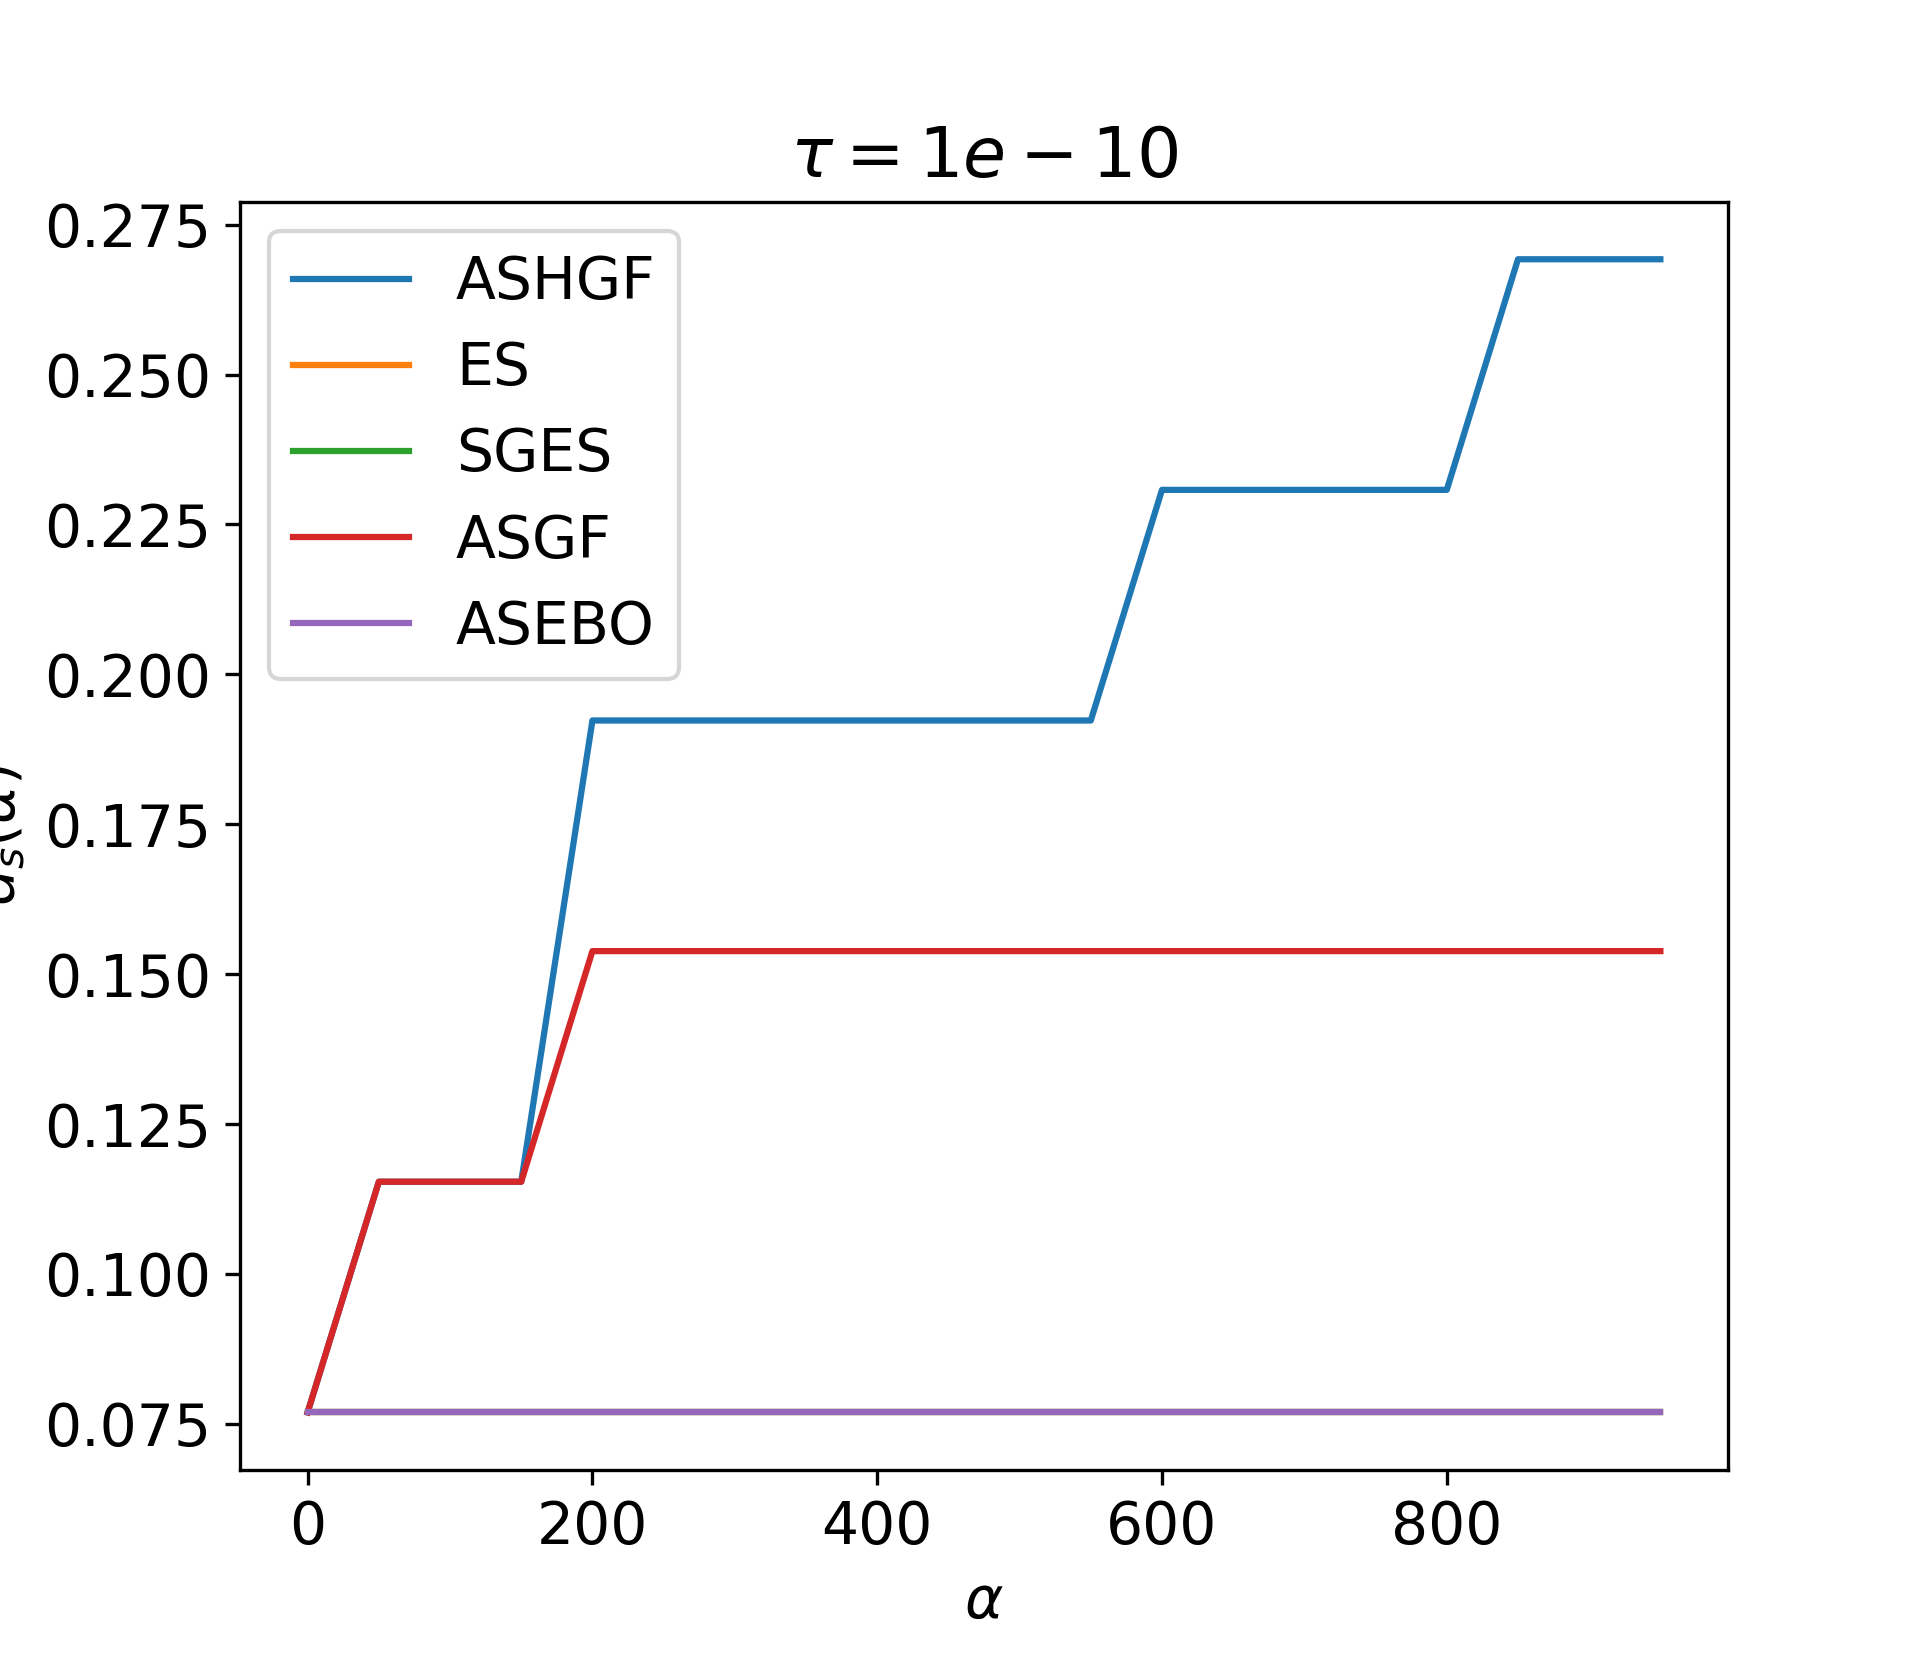
\includegraphics[width=1\textwidth]{figures/data_profiles/1000/data_profile_1000_100000000_1e-10.png}
	\end{subfigure}
	\caption{Data profiles with $\mu_L = 10^{8}$}
	\label{DataProfiles1000Mu100000000}
\end{figure}

\subsection{Statistical analysis of the convergence}

In order to understand the robustness of the algorithm varying the random seed, four of the previously defined functions were selected, namely: \textit{Sphere}, \textit{Rastrigin}, \textit{Levy} and \textit{Ackley}; they were optimized using ASHGF with one hundred different random seeds, the same for each function.

\begin{figure}[H]
	\centering
	\begin{subfigure}{0.39\textwidth}
		\centering 
		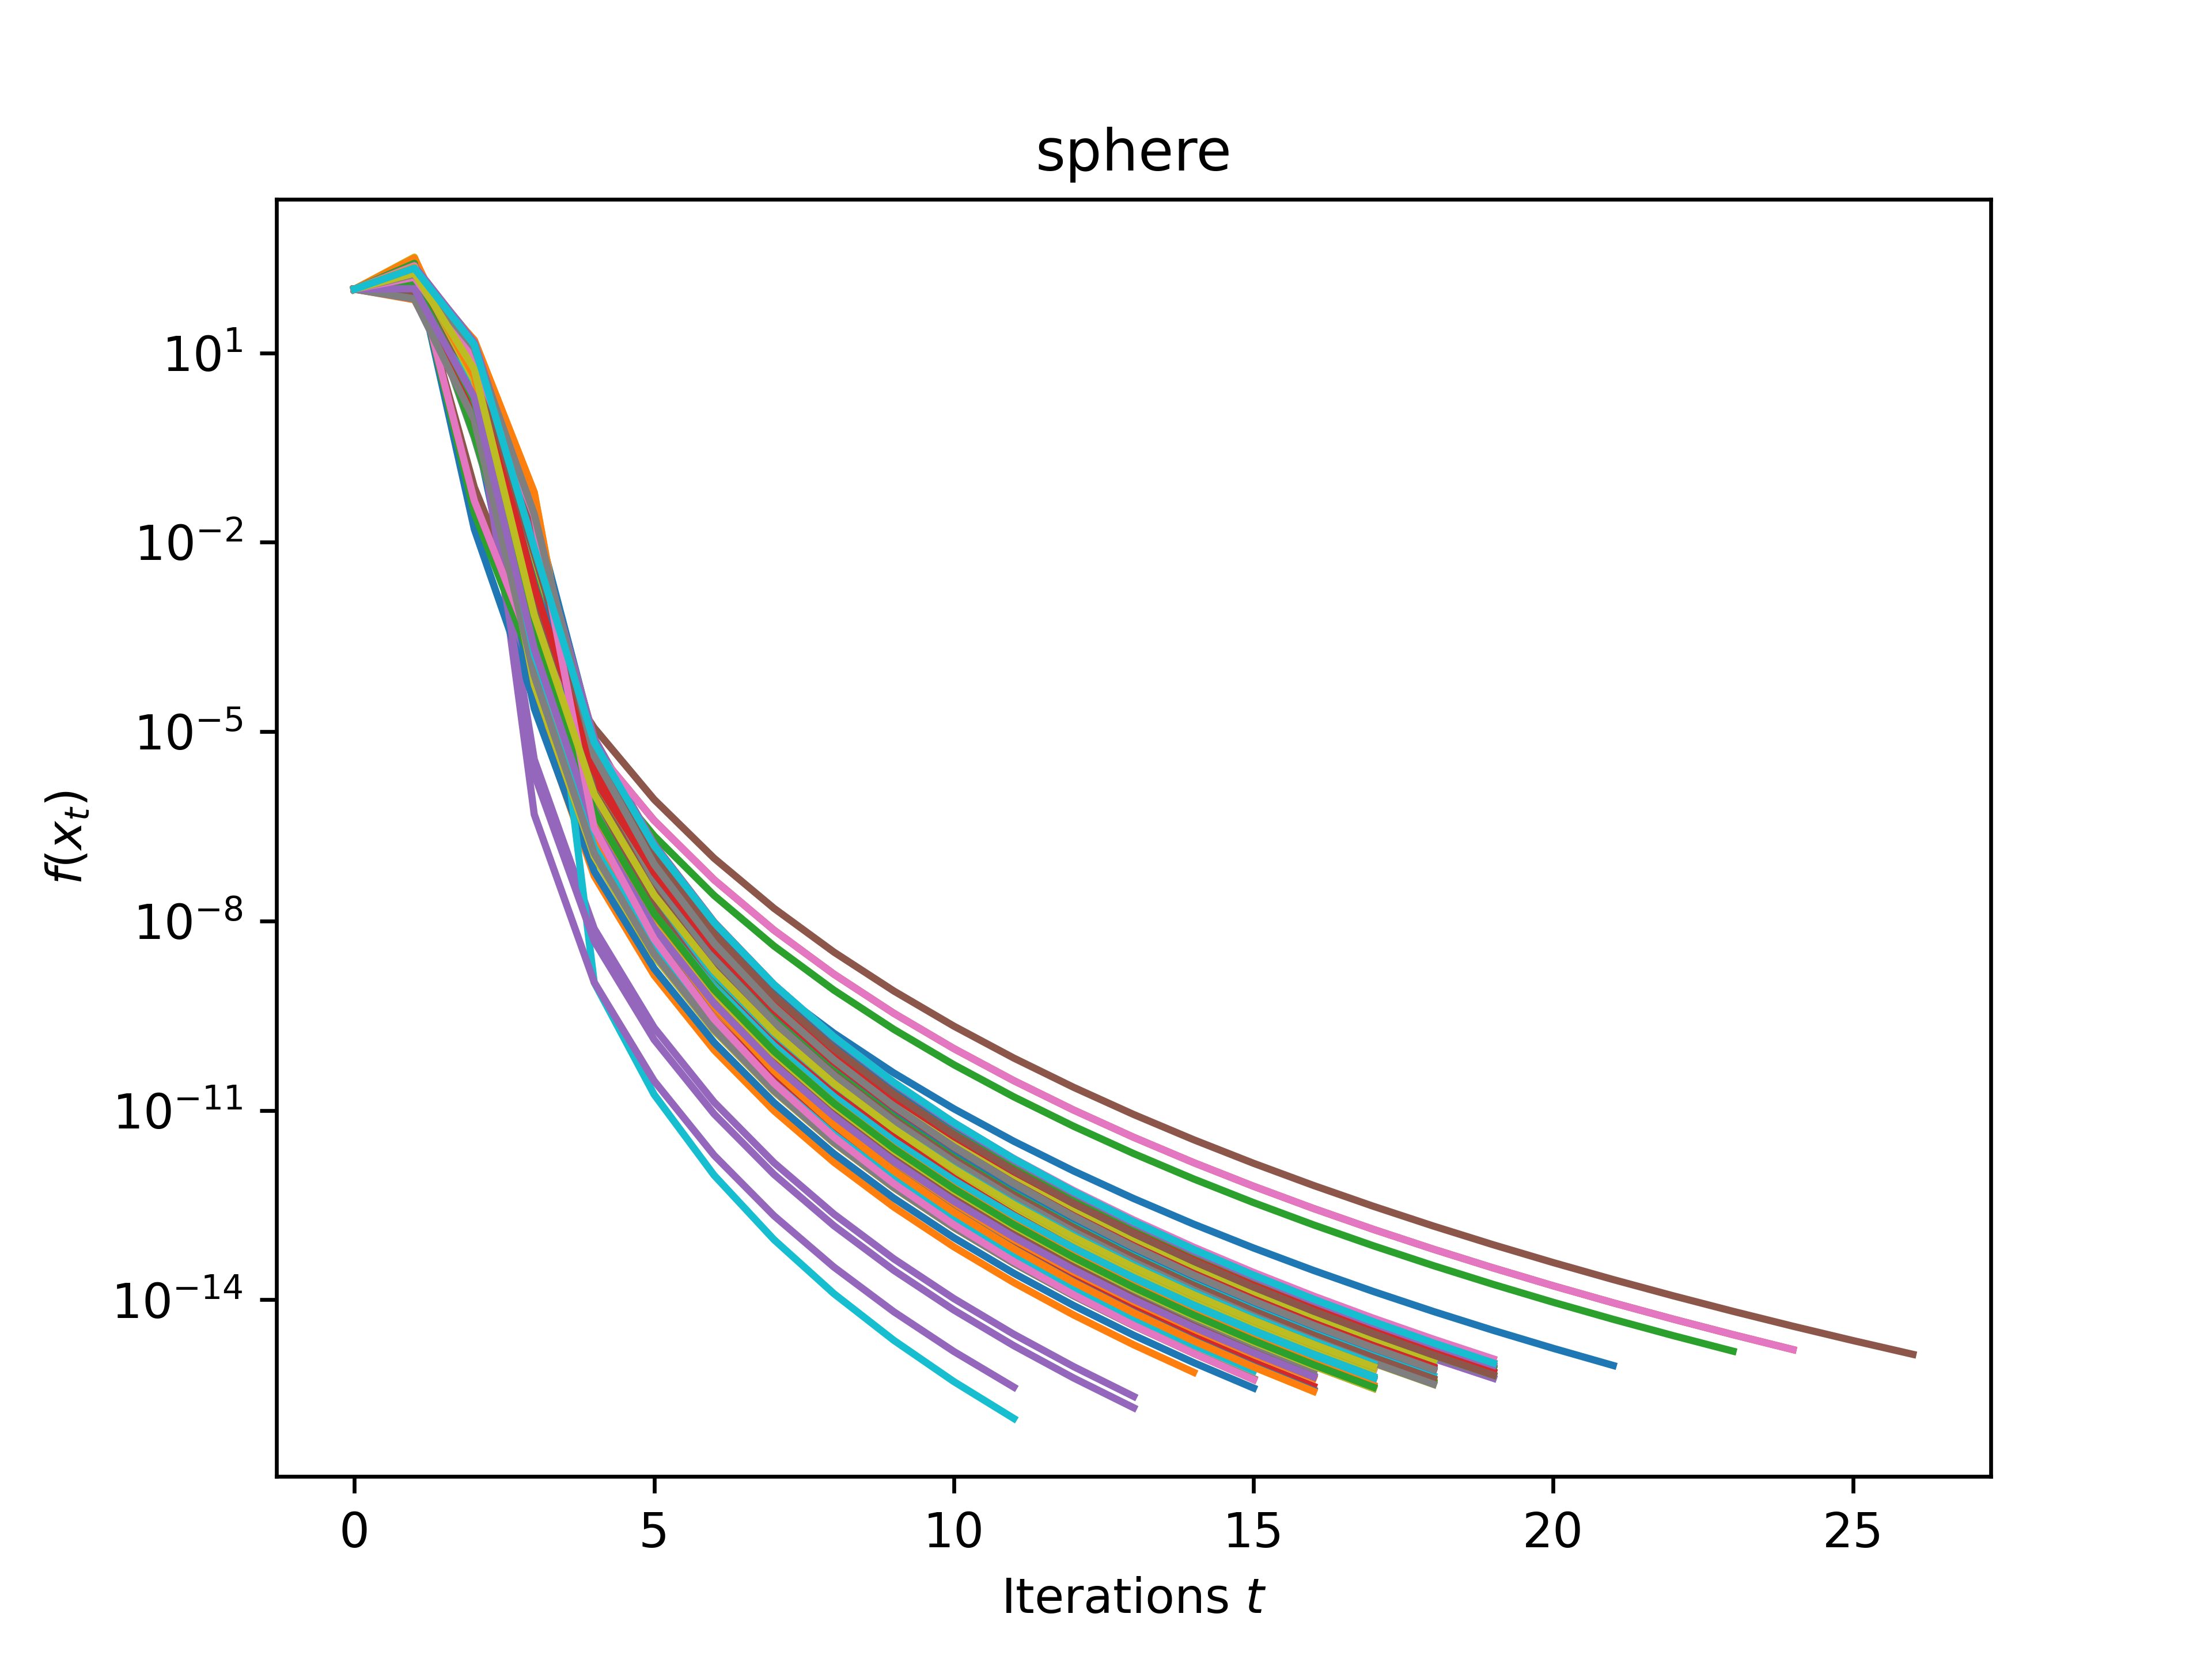
\includegraphics[width=1\textwidth]{figures/average_descent/ASHGF/sphere_convergence.png}
	\end{subfigure}%
	\begin{subfigure}{0.39\textwidth}
		\centering 
		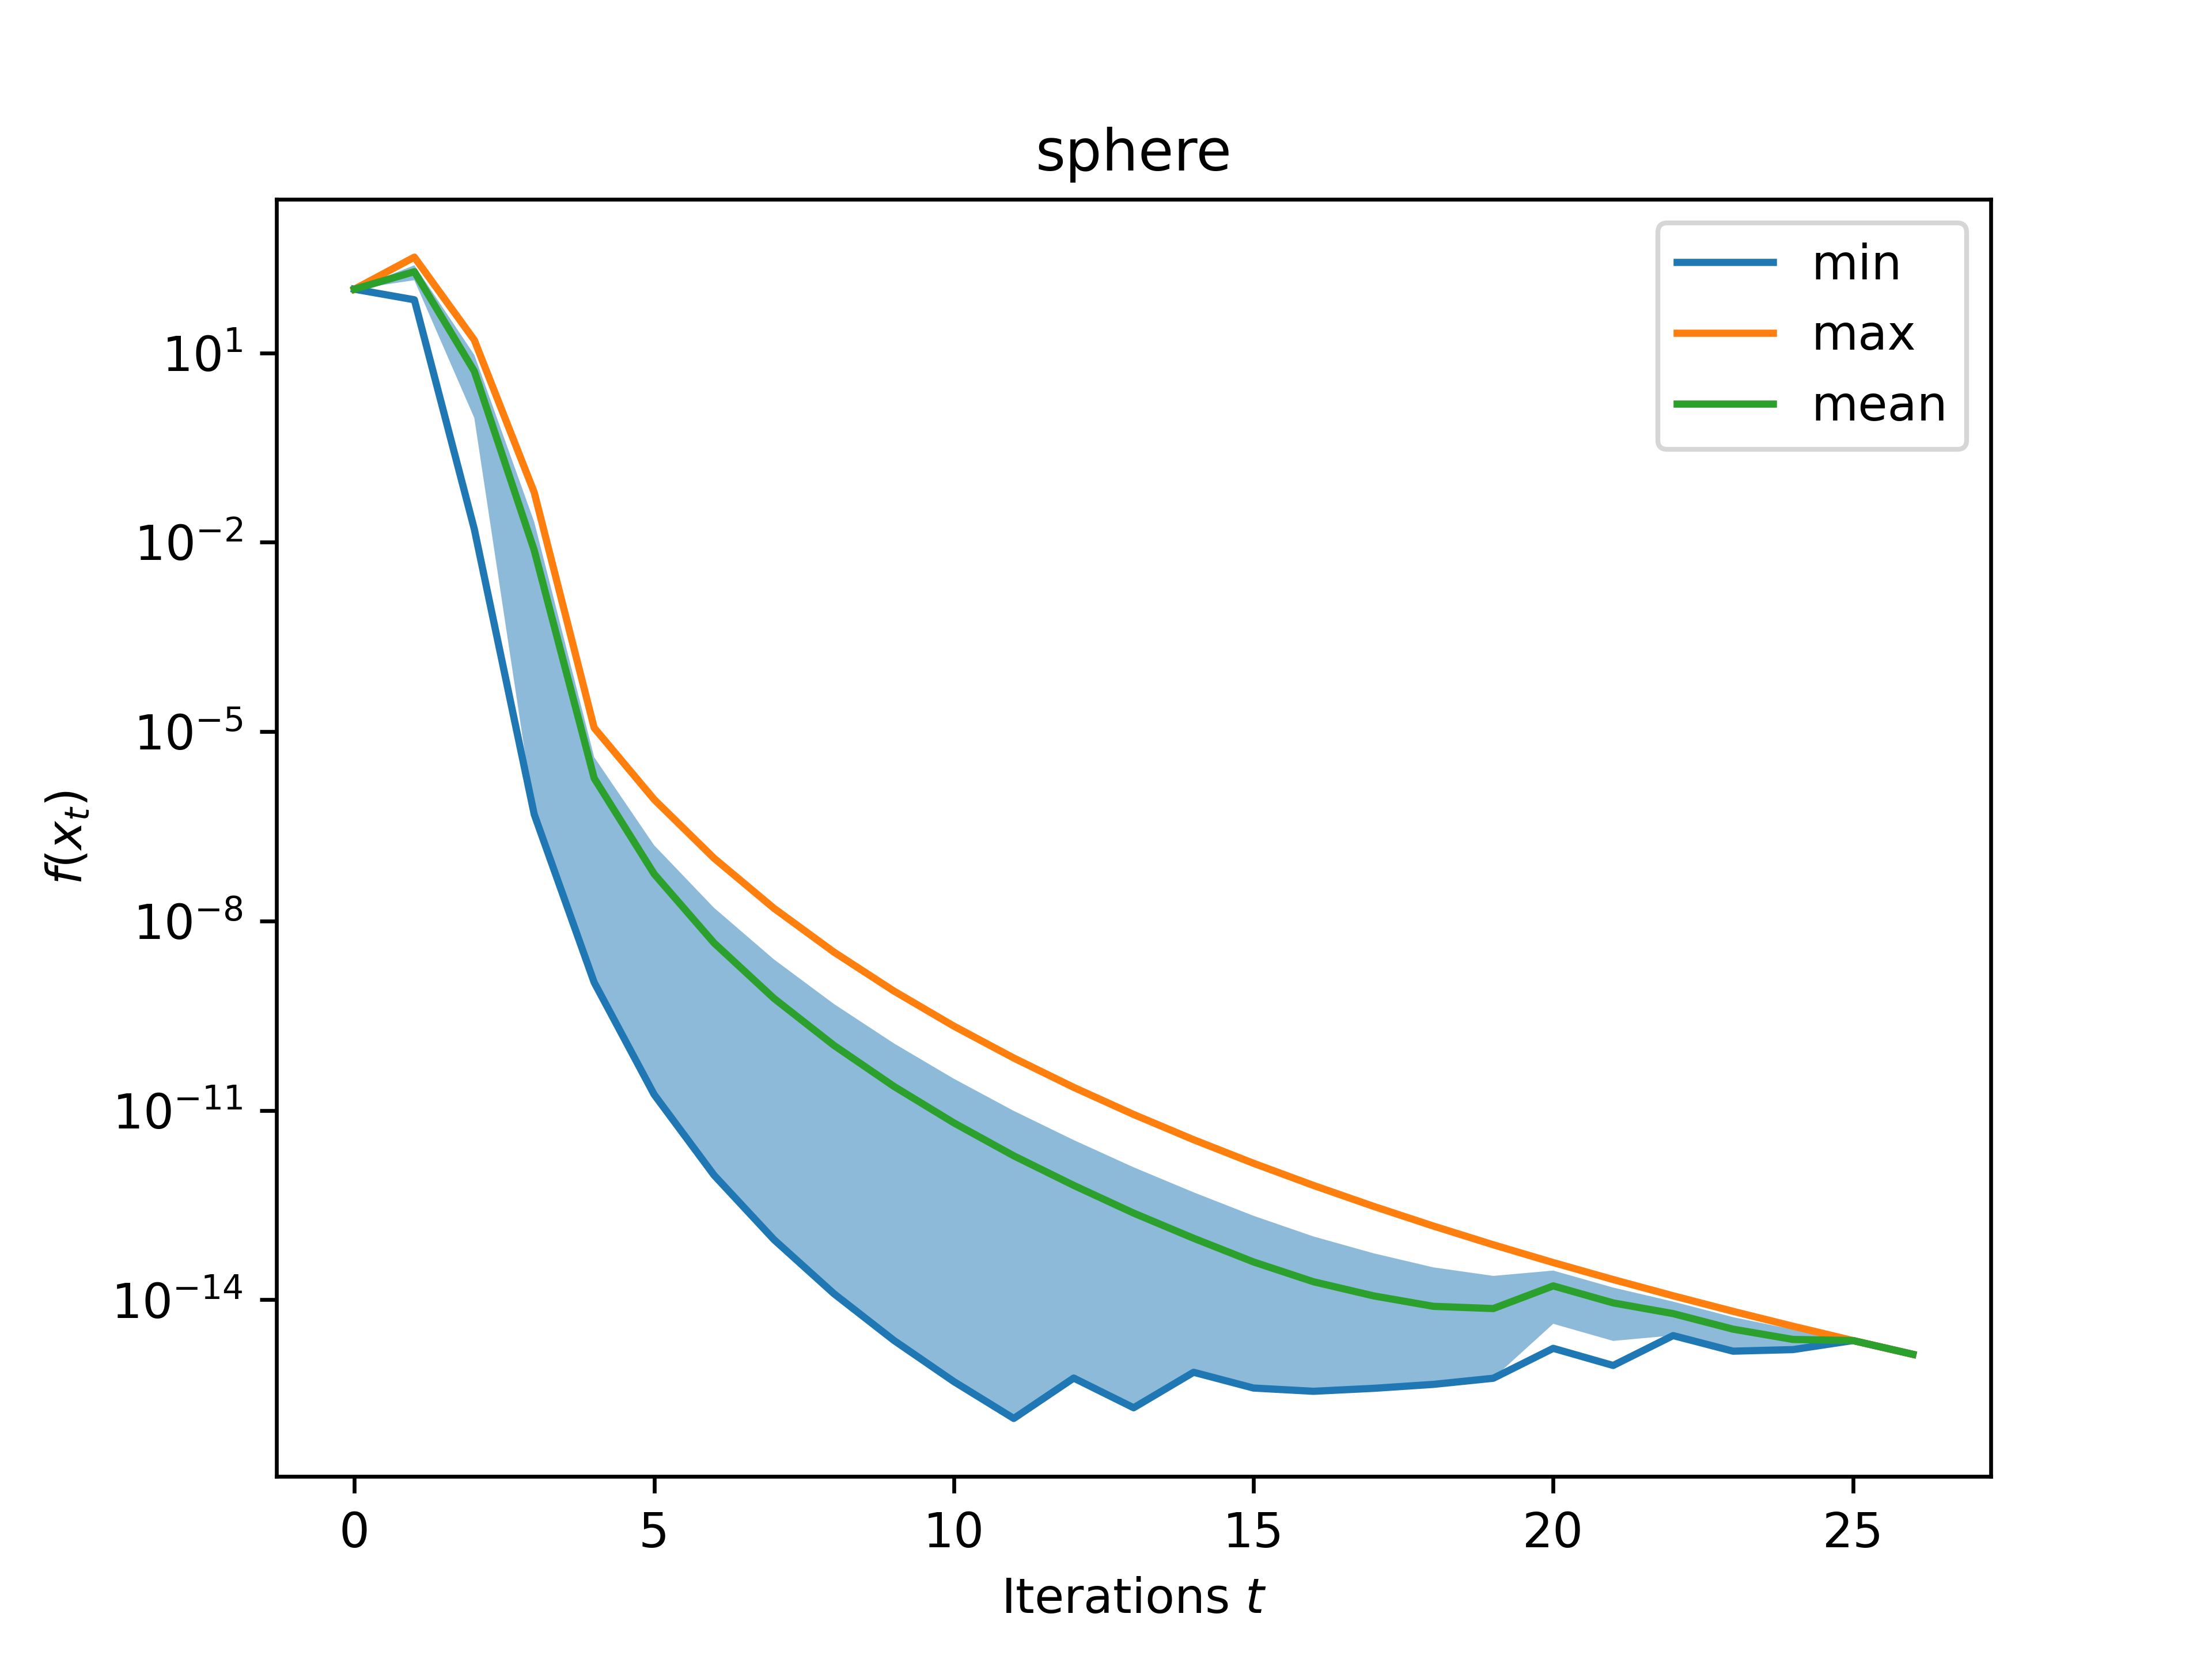
\includegraphics[width=1\textwidth]{figures/average_descent/ASHGF/sphere_convergence_mean.png}
	\end{subfigure}
	\begin{subfigure}{0.39\textwidth}
		\centering 
		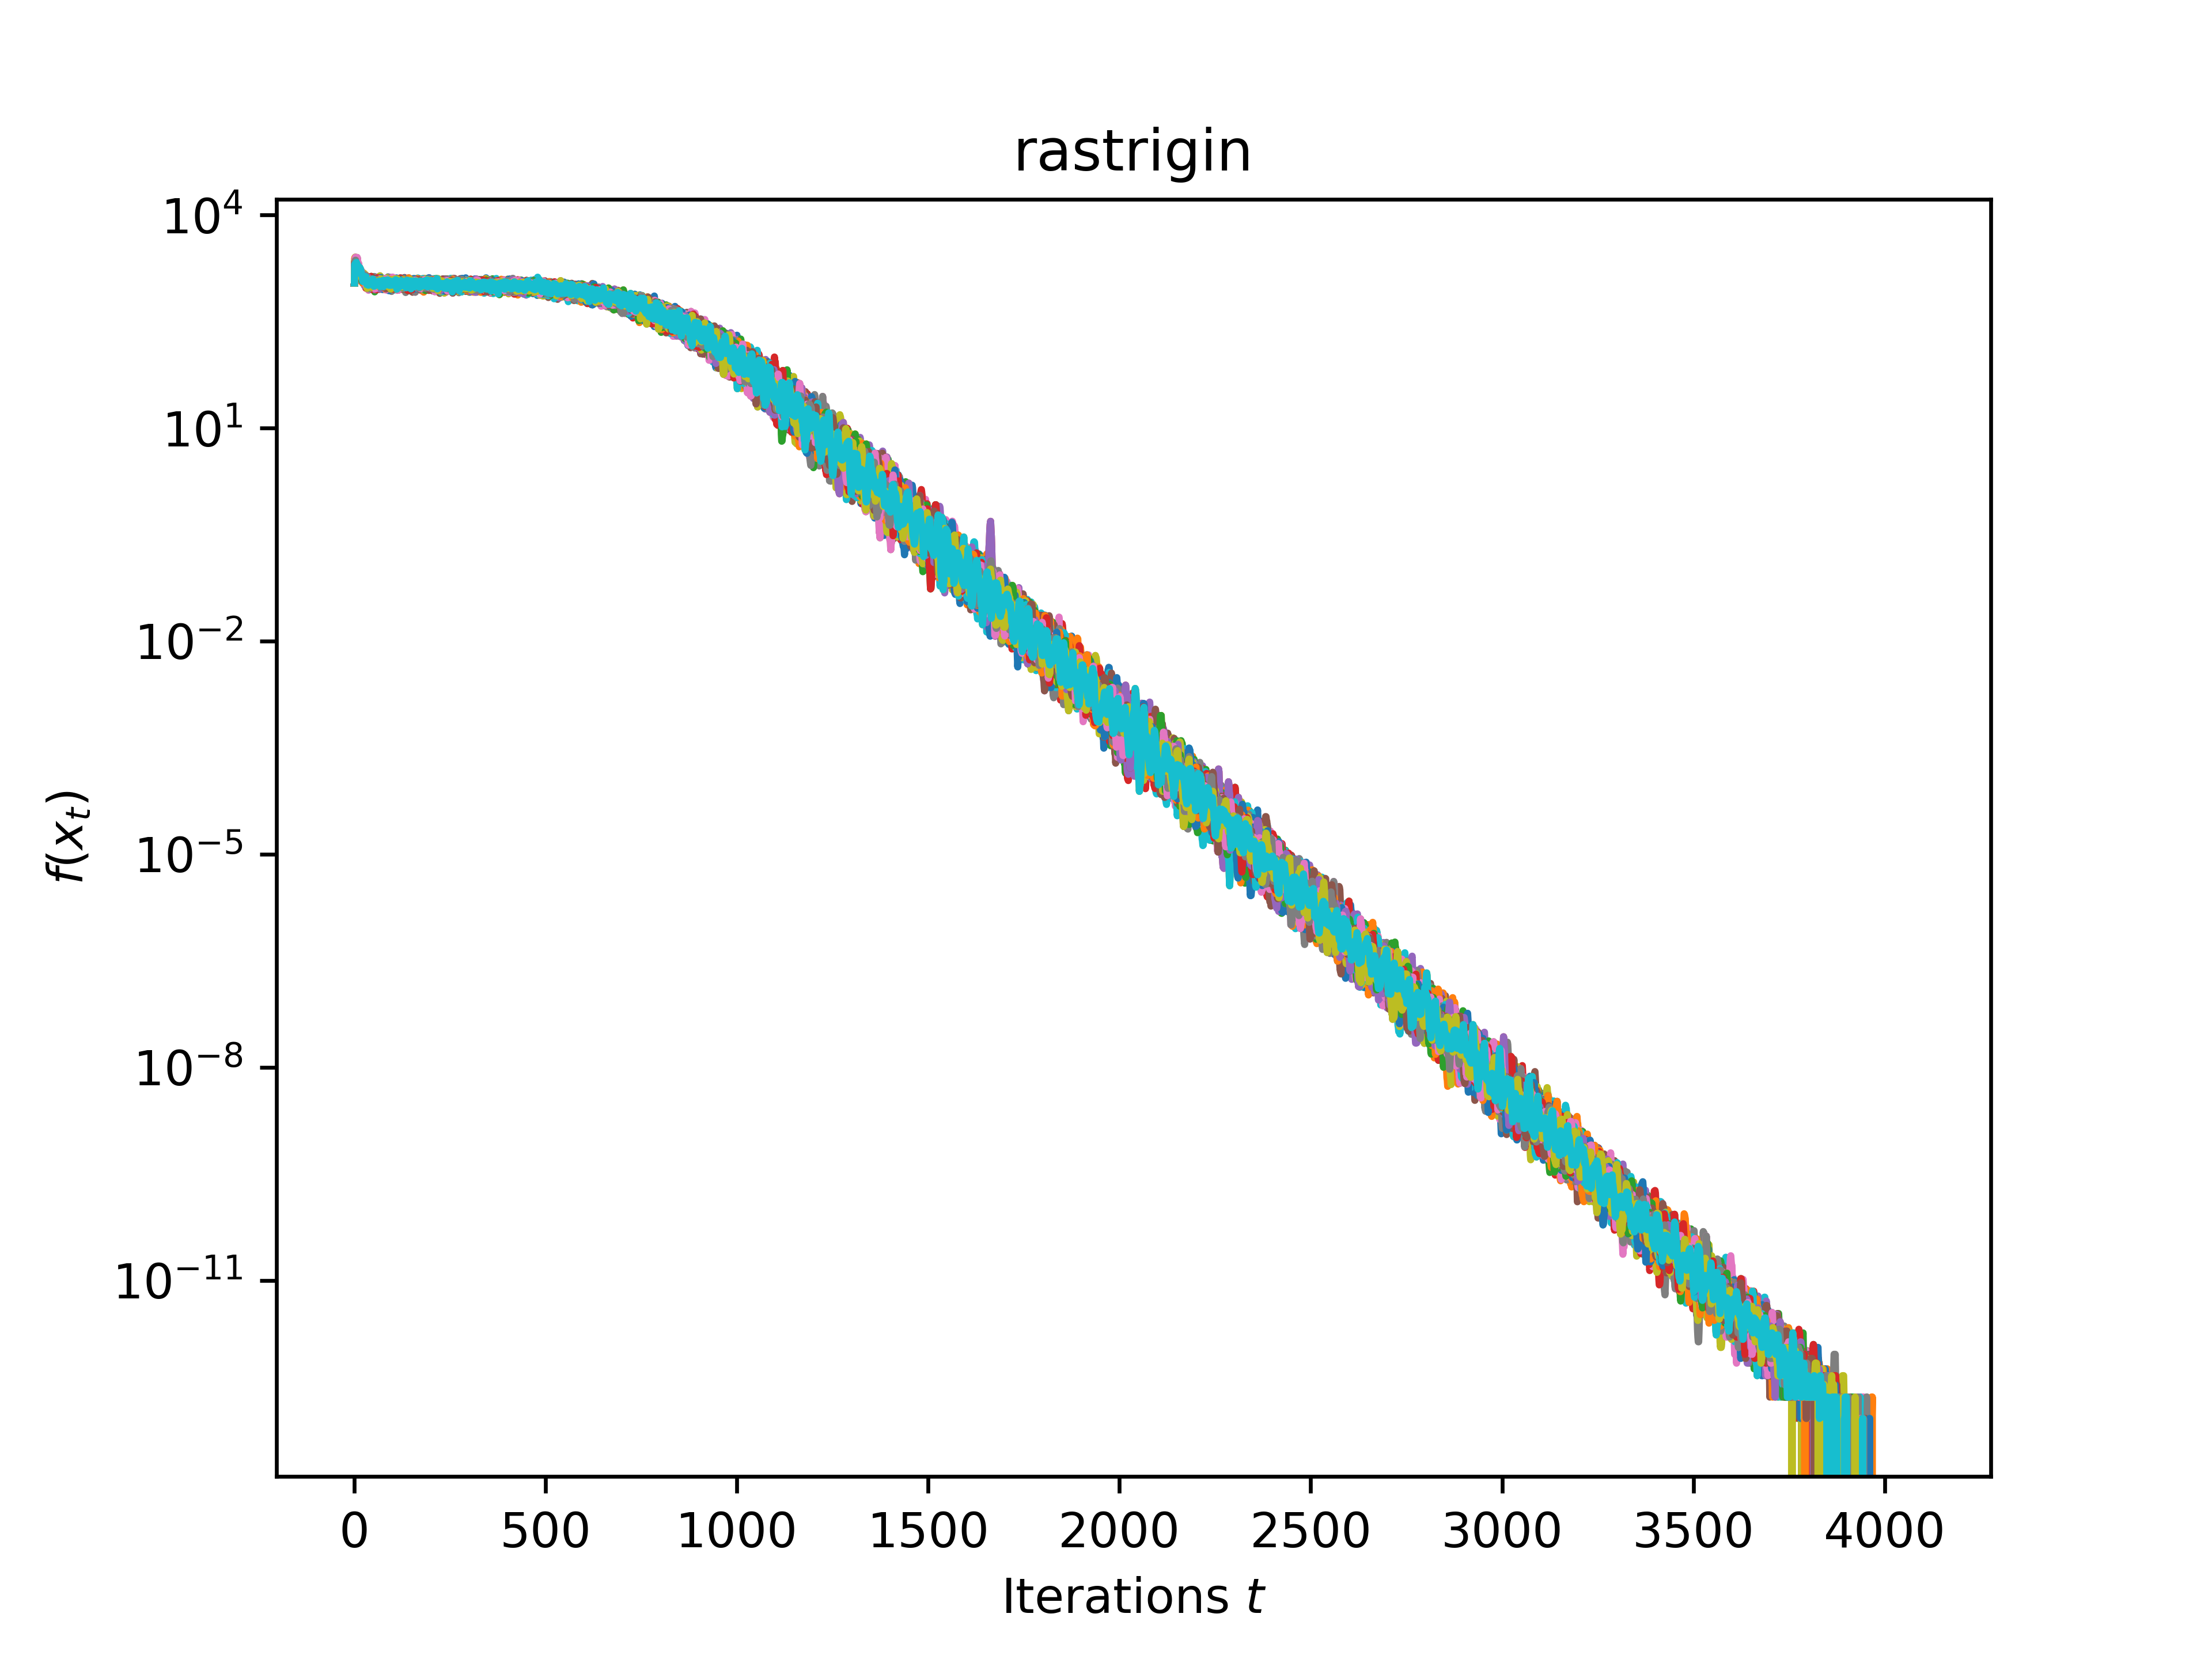
\includegraphics[width=1\textwidth]{figures/average_descent/ASHGF/rastrigin_convergence.png}
	\end{subfigure}%
	\begin{subfigure}{0.39\textwidth}
		\centering 
		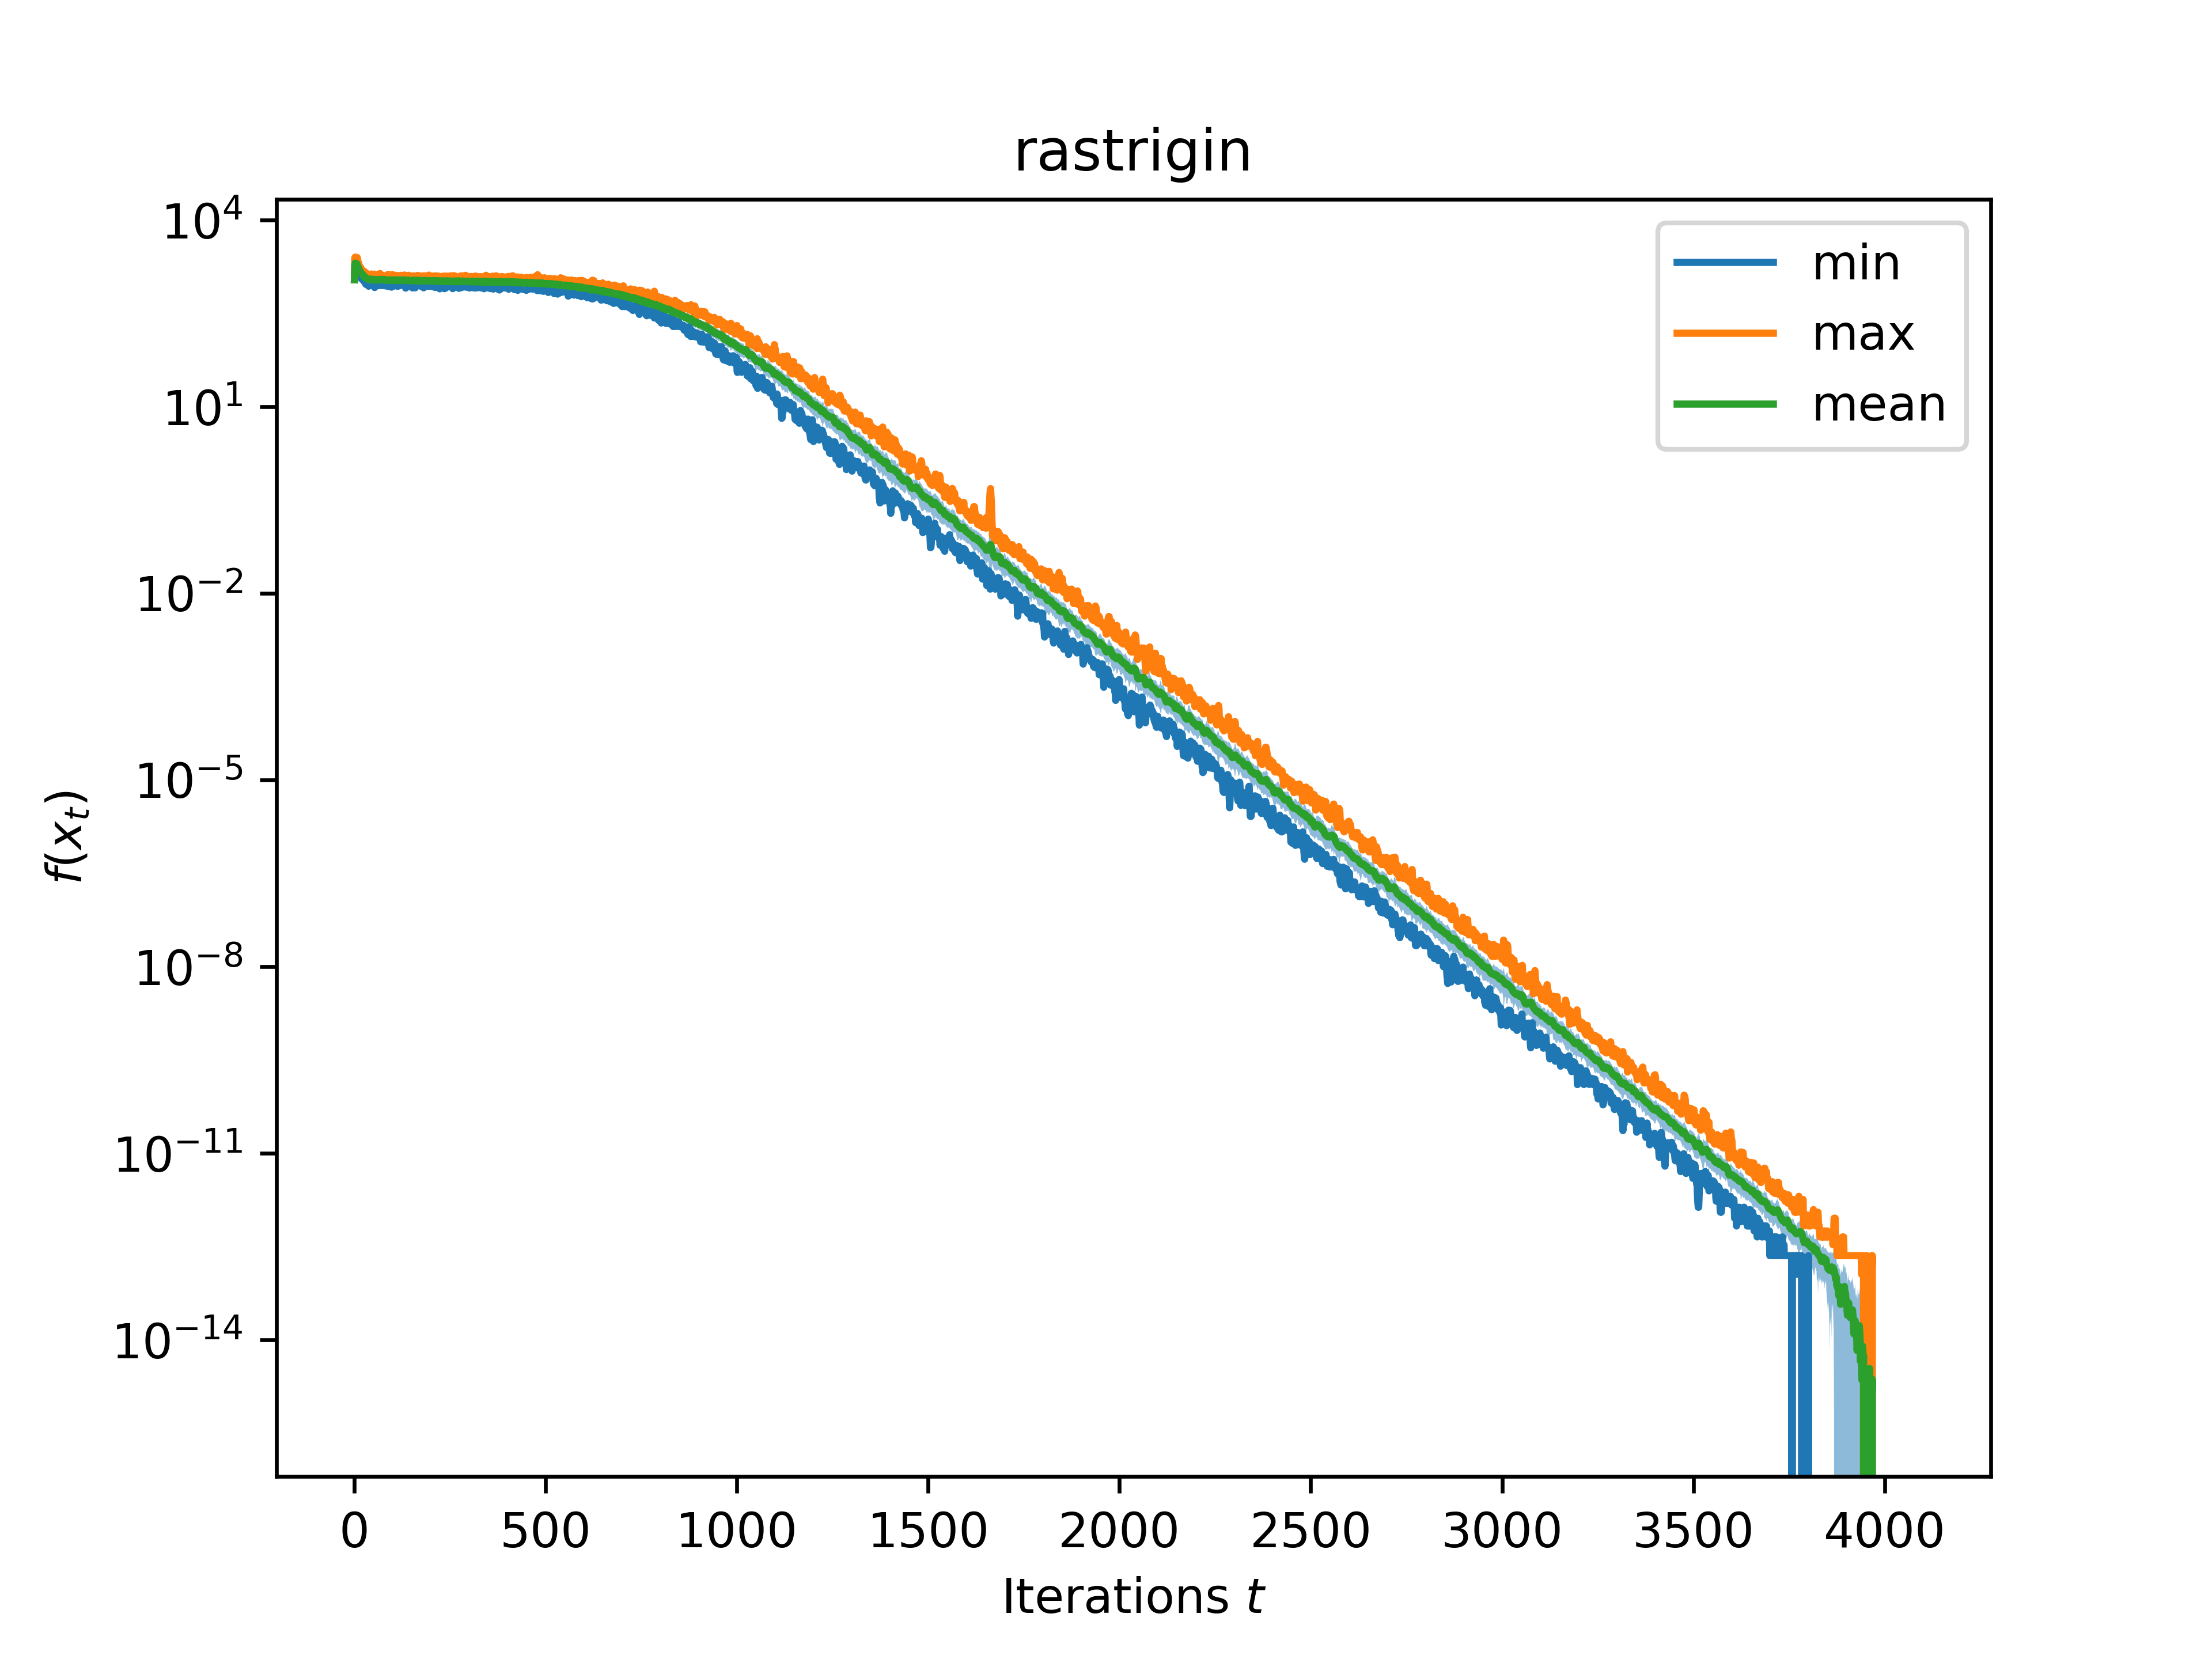
\includegraphics[width=1\textwidth]{figures/average_descent/ASHGF/rastrigin_convergence_mean.png}
	\end{subfigure}
	\begin{subfigure}{0.39\textwidth}
		\centering 
		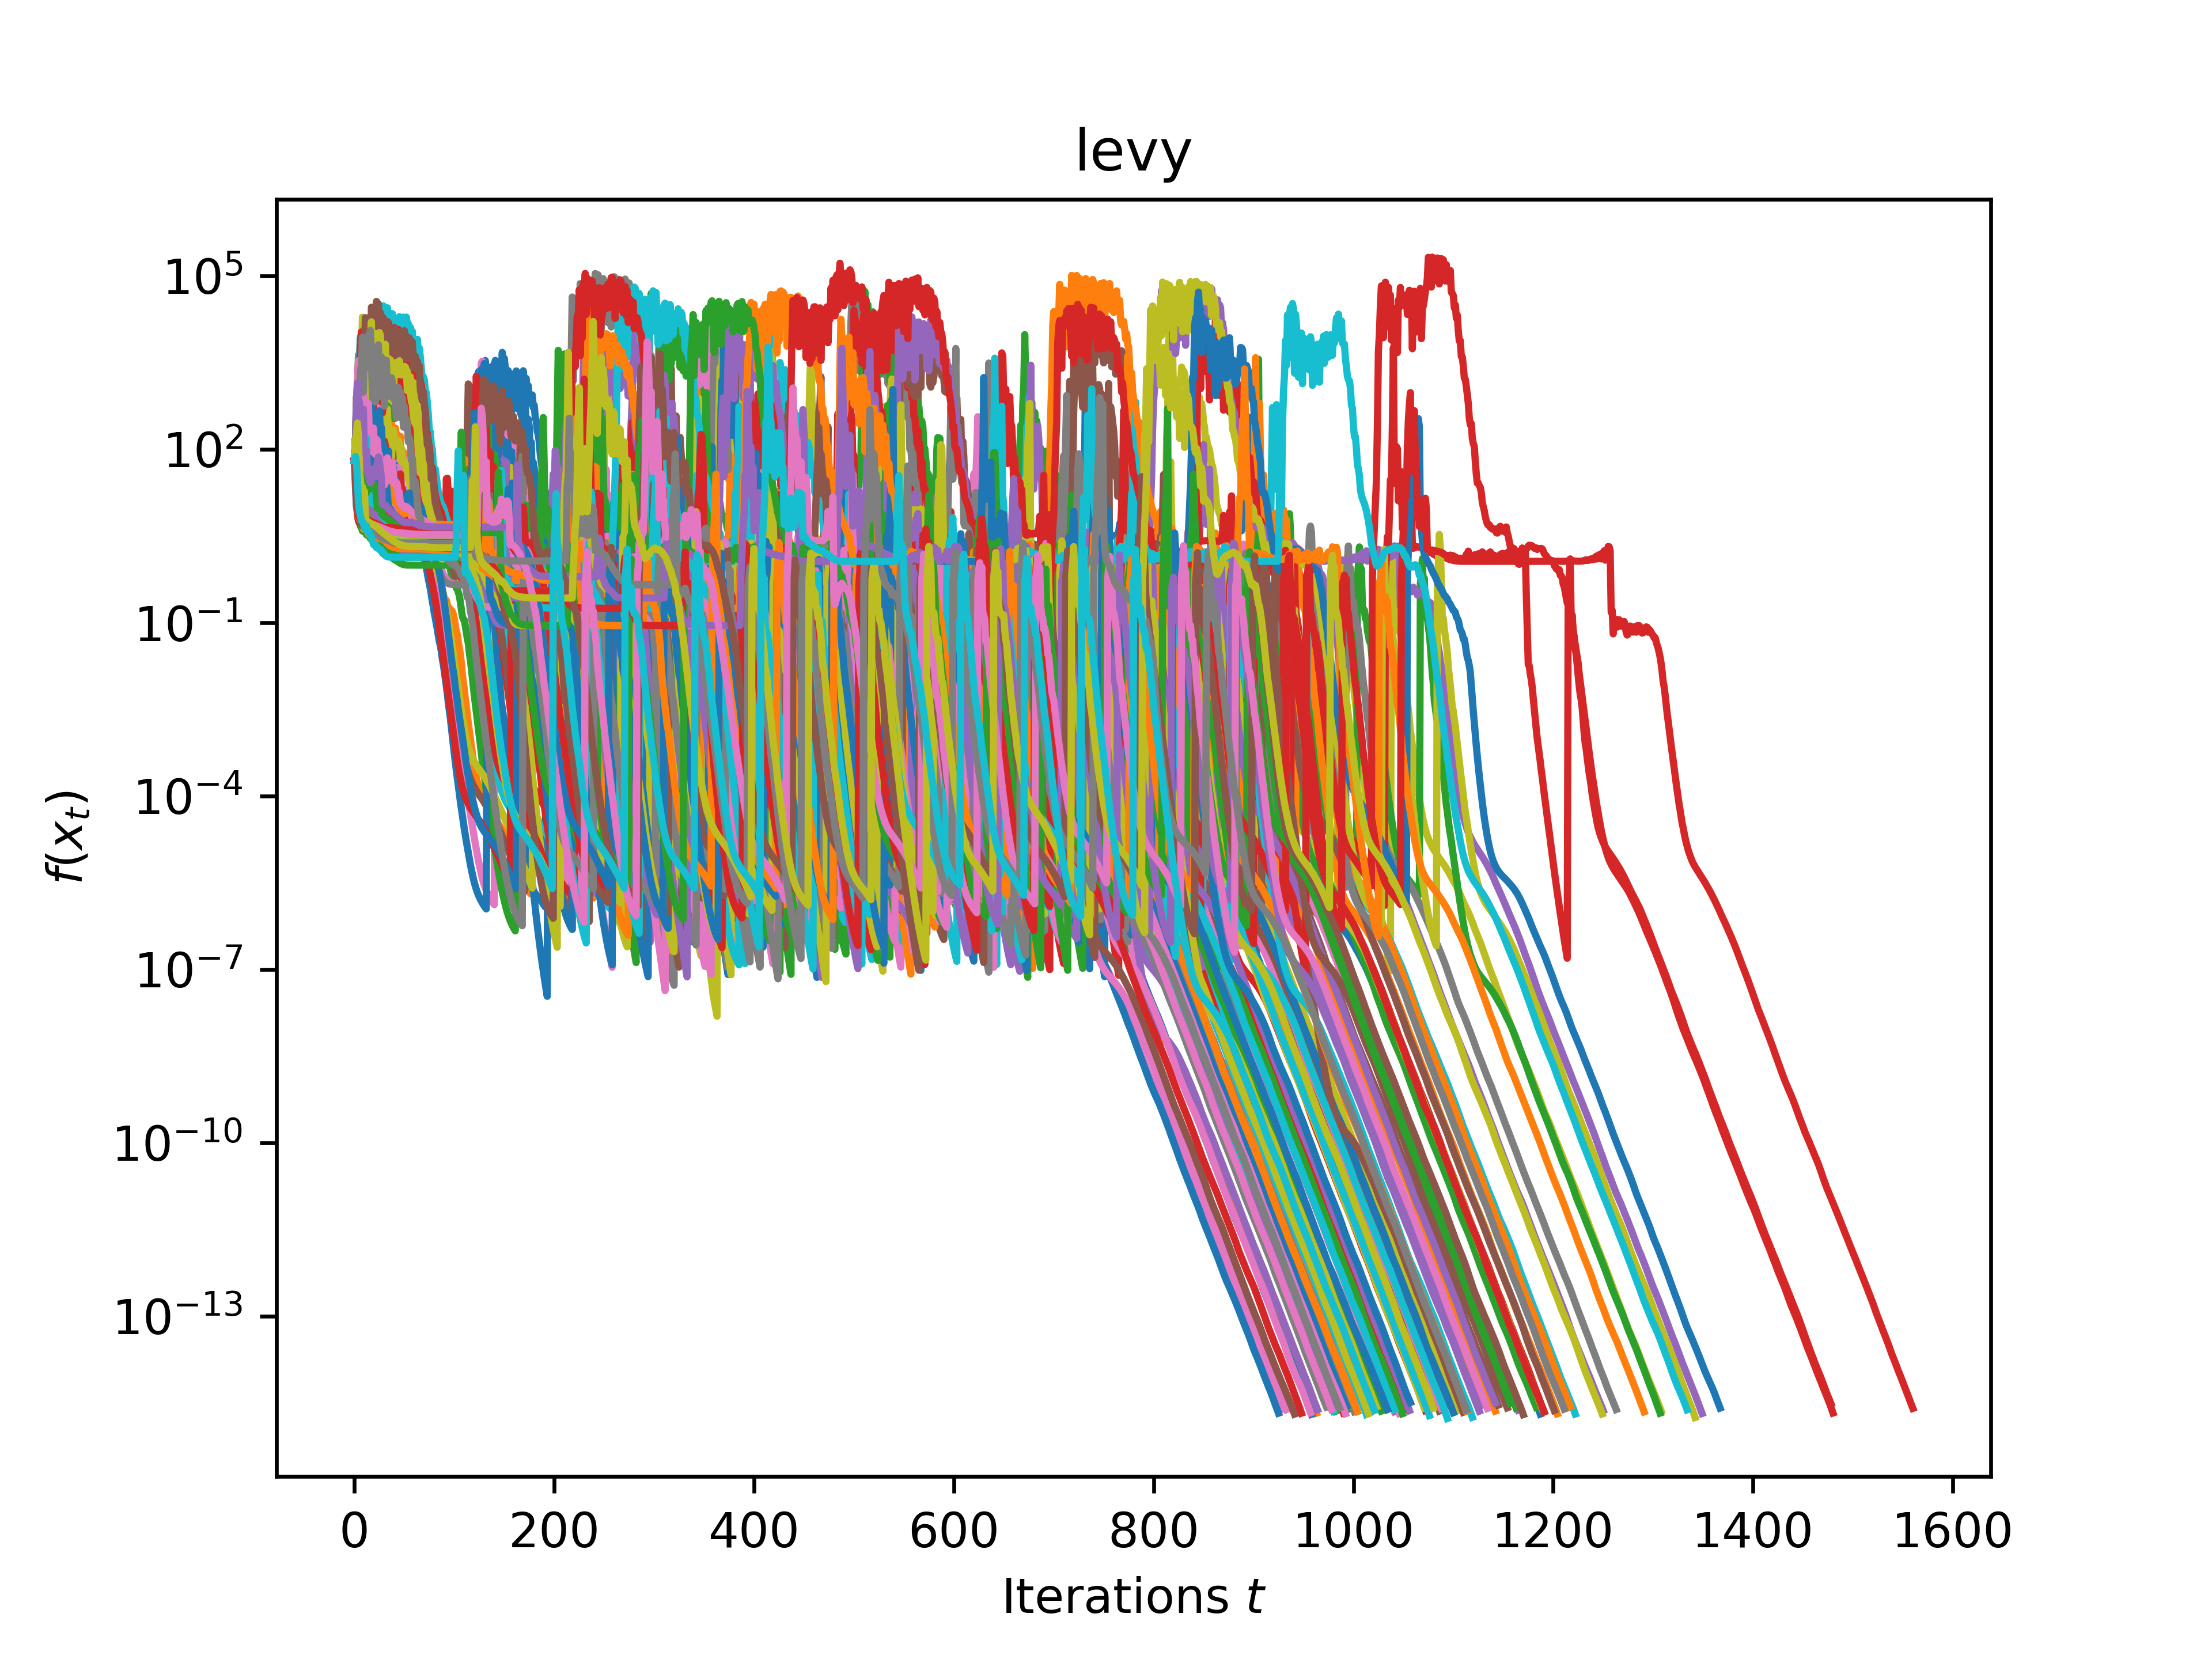
\includegraphics[width=1\textwidth]{figures/average_descent/ASHGF/levy_convergence.png}
	\end{subfigure}%
	\begin{subfigure}{0.39\textwidth}
		\centering 
		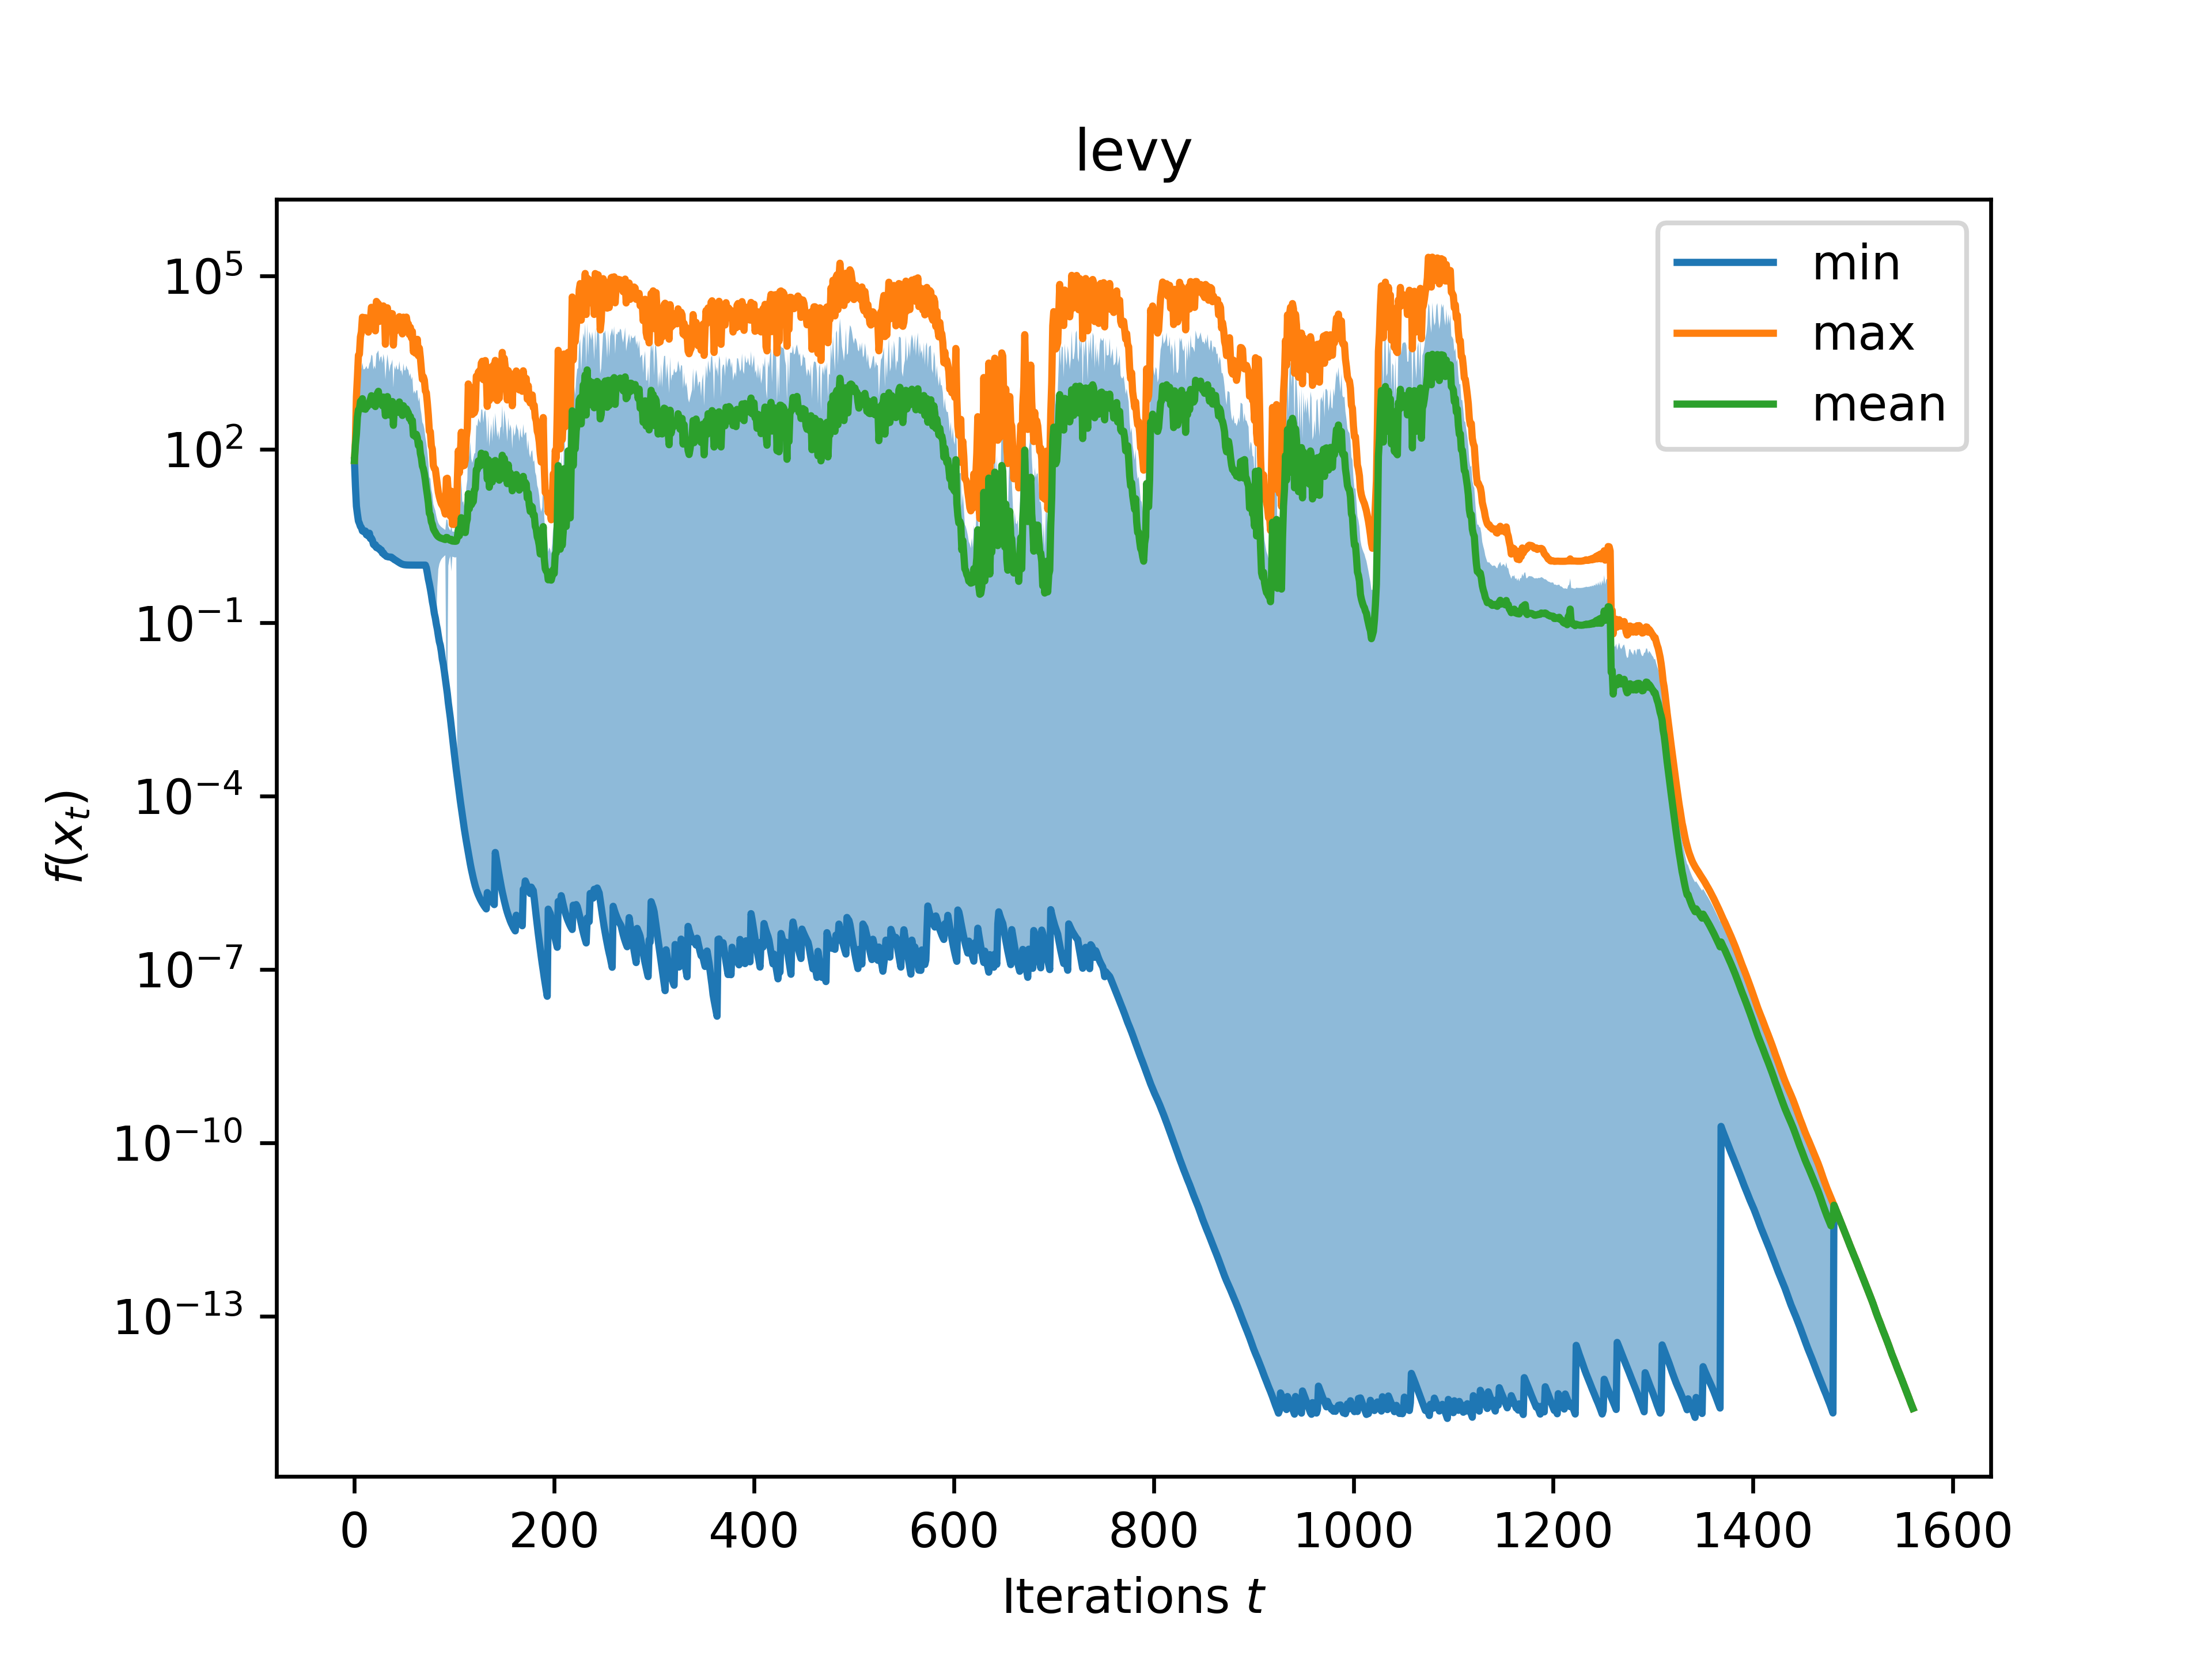
\includegraphics[width=1\textwidth]{figures/average_descent/ASHGF/levy_convergence_mean.png}
	\end{subfigure}
	\begin{subfigure}{0.39\textwidth}
		\centering 
		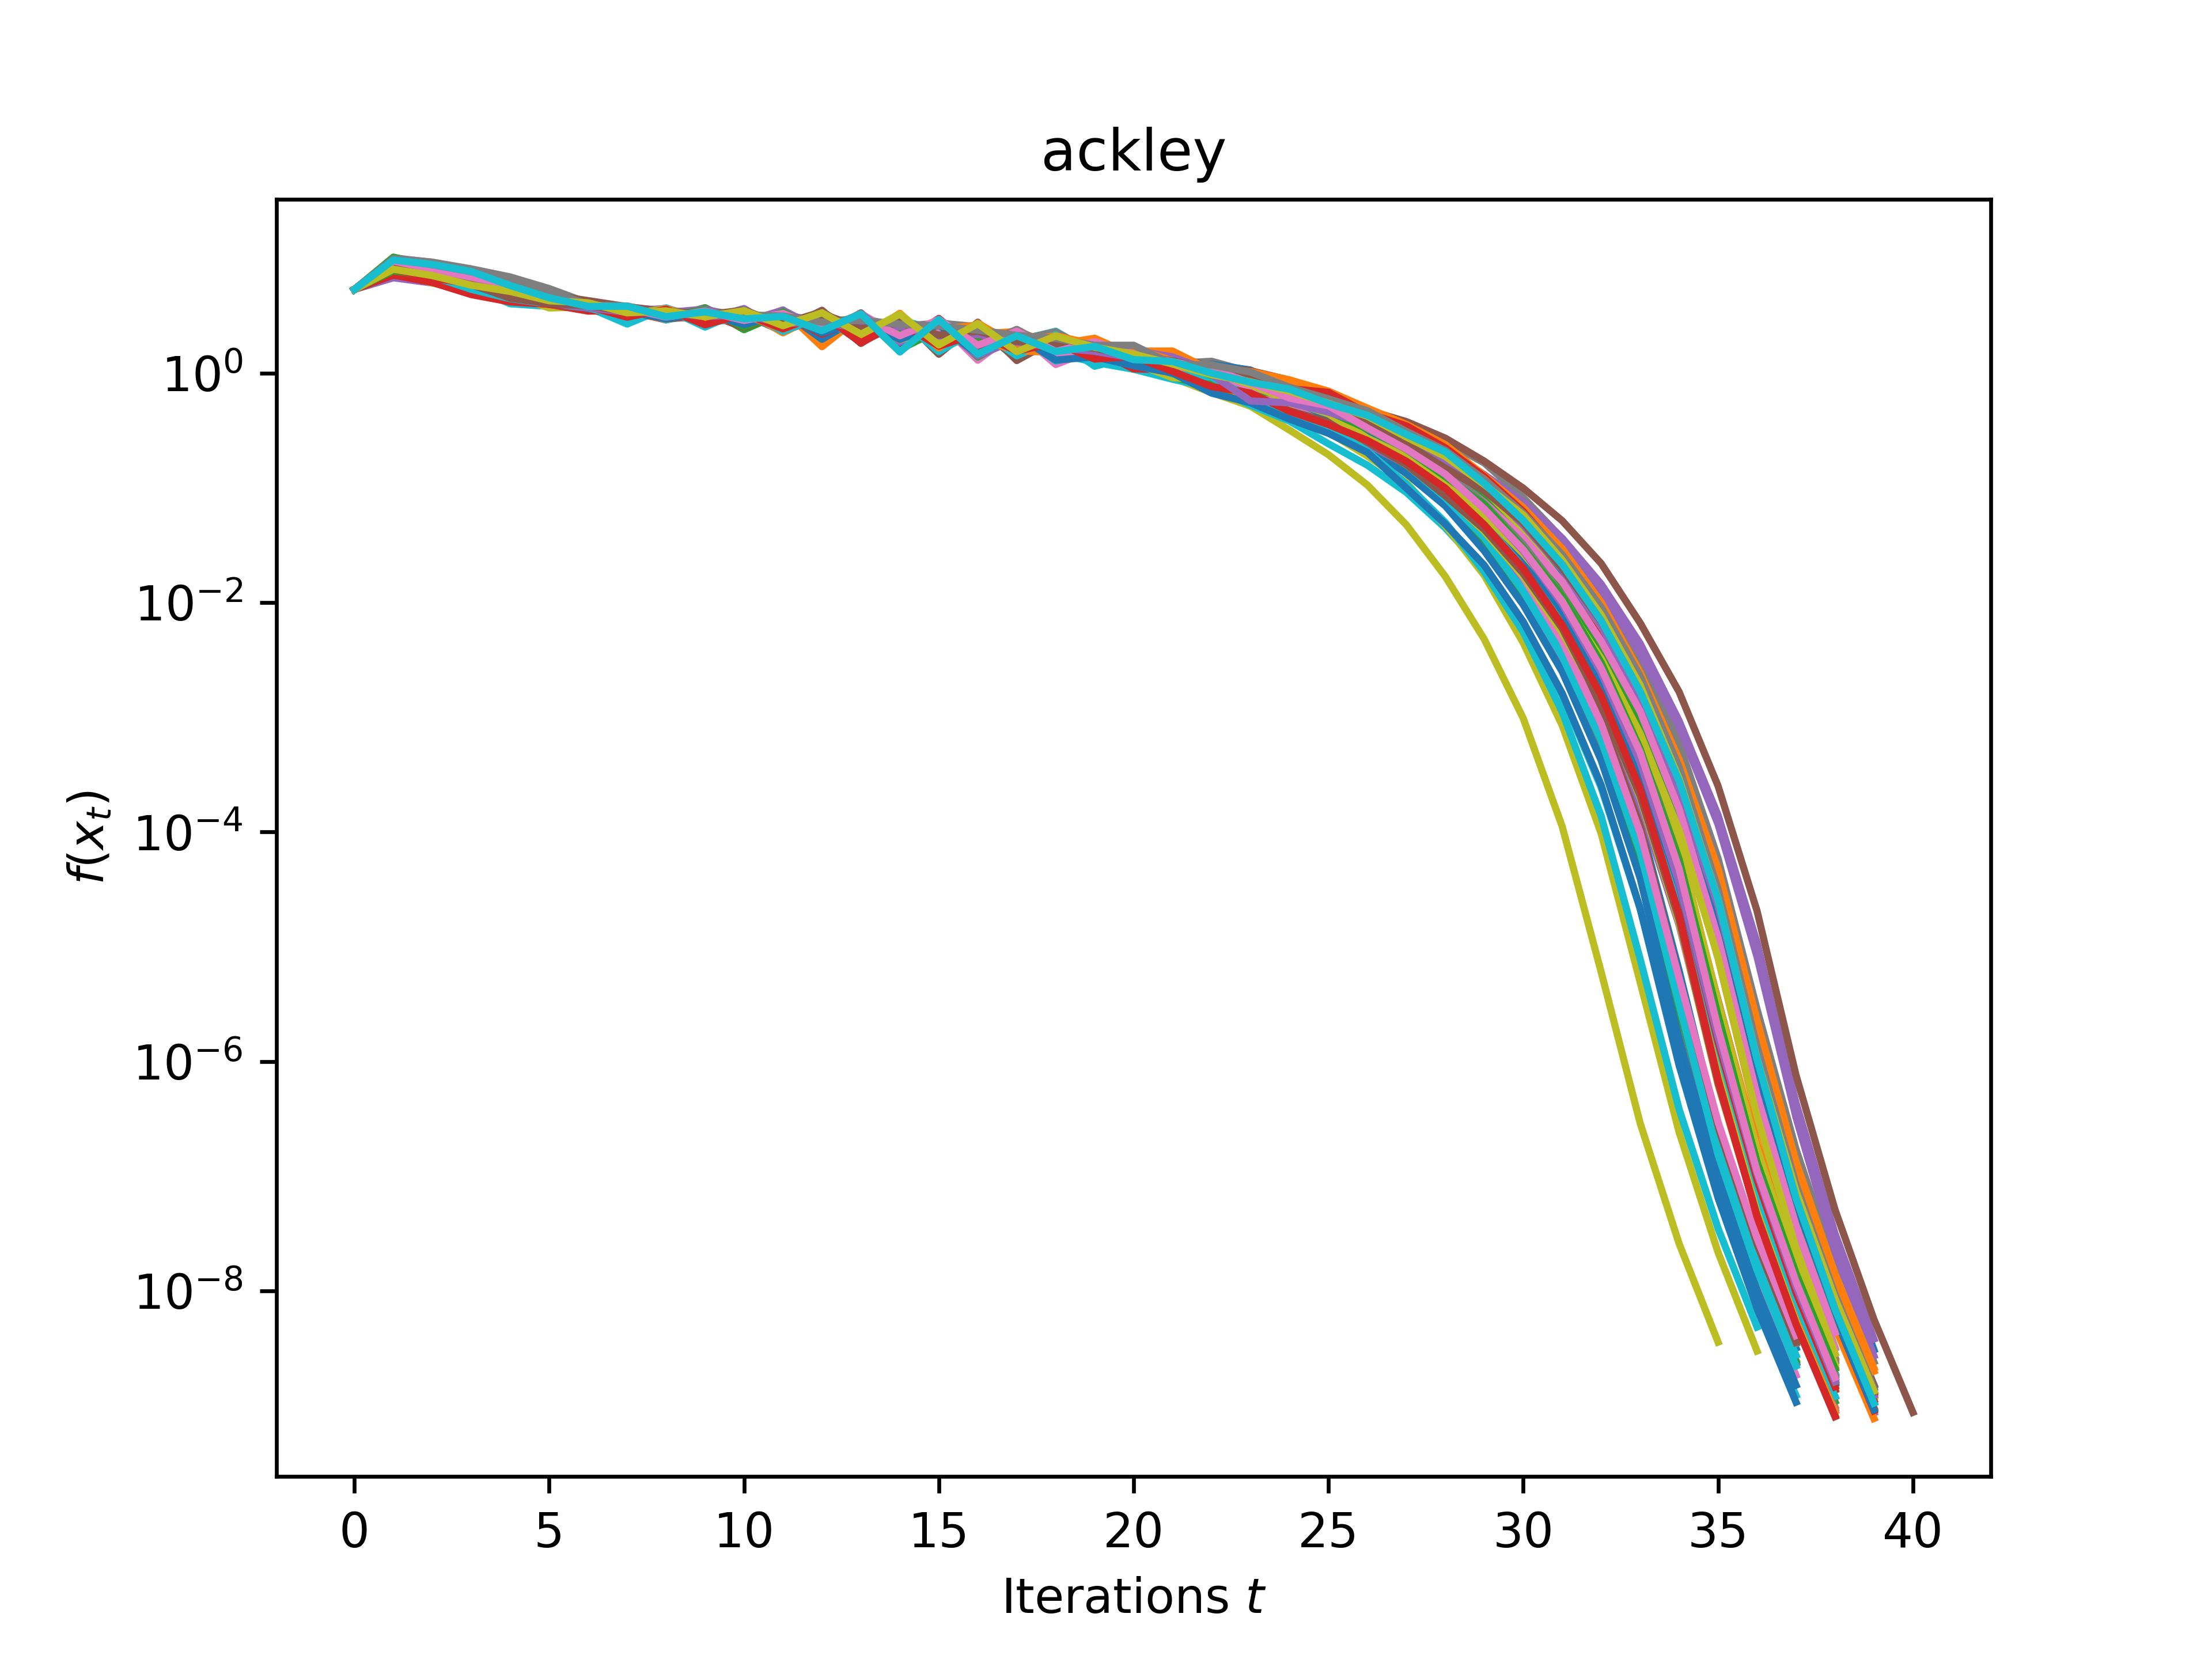
\includegraphics[width=1\textwidth]{figures/average_descent/ASHGF/ackley_convergence.png}
	\end{subfigure}%
	\begin{subfigure}{0.39\textwidth}
		\centering 
		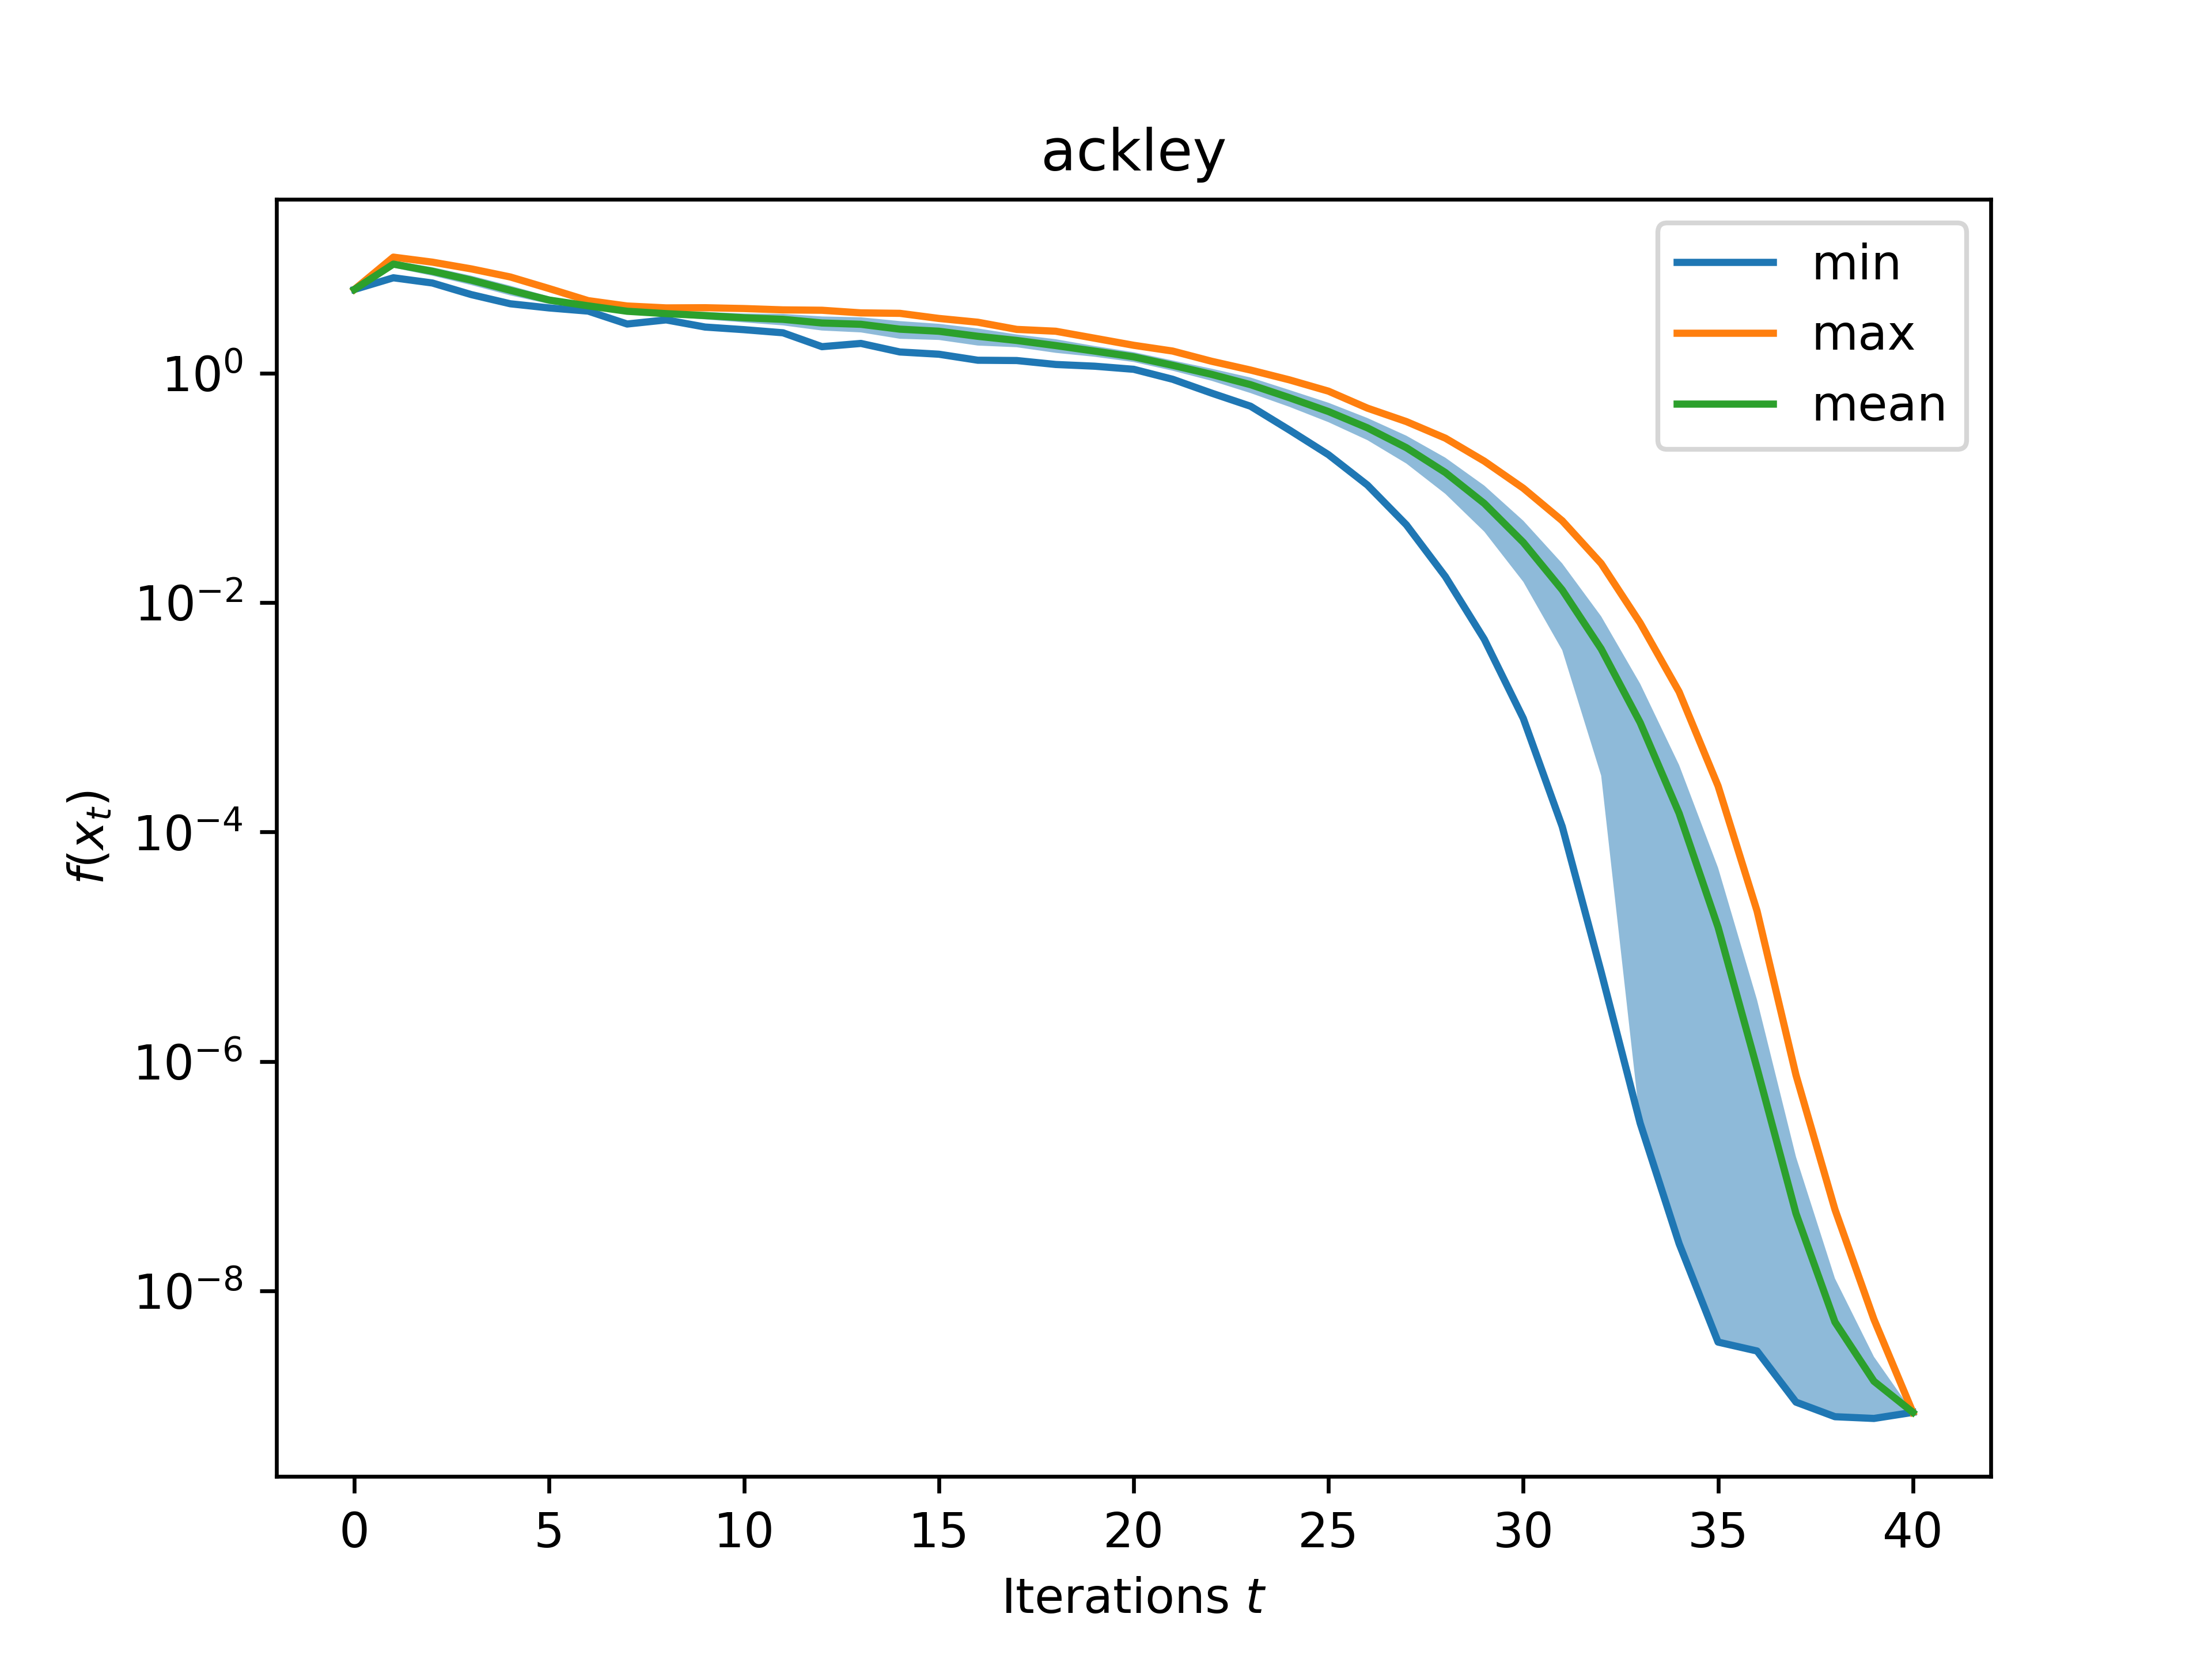
\includegraphics[width=1\textwidth]{figures/average_descent/ASHGF/ackley_convergence_mean.png}
	\end{subfigure}
	\caption[Average results of optimization]{Results of the optimization of the functions \textit{Sphere}, \textit{Rastrigin}, \textit{Levy} and \textit{Ackley} on $100$ different random seeds. The figures on the left show all the function decay. The figures on the right show the slowest, fastest and average decay, with the highlighted area being the standard deviation from the mean.}
	\label{AverageResults}
\end{figure}

The algorithm converged for each seed and function. The dimension of choice was $100$, being both high enough while still being feasible in terms of computational times. As expected, with \textit{Sphere}, a strongly convex function, the algorithm converged in a very small number of iterations.

In the following figures the presented algorithm is compared in its average run on $100$ random seeds, on the same functions as in \ref{AverageResults}, against \ref{ESAlgorithm}, \ref{ASEBO}, \ref{SGES} and \ref{ASGF}.

\begin{figure}[H]
	\centering
	\begin{subfigure}{0.4\textwidth}
		\centering 
		
\includegraphics[width=1\textwidth]{figures/average_descent_compared/sphere_convergence_mean.png}
	\end{subfigure}
	\begin{subfigure}{0.4\textwidth}
		\centering 
		
\includegraphics[width=1\textwidth]{figures/average_descent_compared/rastrigin_convergence_mean.png}
	\end{subfigure}
	\begin{subfigure}{0.4\textwidth}
		\centering 
		
\includegraphics[width=1\textwidth]{figures/average_descent_compared/levy_convergence_mean.png}
	\end{subfigure}
	\begin{subfigure}{0.4\textwidth}
		\centering 
		
\includegraphics[width=1\textwidth]{figures/average_descent_compared/ackley_convergence_mean.png}
	\end{subfigure}
	\caption[Comparison of average optimization results between algorithms.]{Results of the optimization of the functions \textit{Sphere}, \textit{Rastrigin}, \textit{Levy} and \textit{Ackley} on $100$ different random seeds for each of the algorithms in \ref{chapt:2}. In the figures are reported the average function decay for each algorithm.}
	\label{AverageDescentsCompared}
\end{figure}

Again, like with the results of the performance and data profiles, the proposed algorithm shows to be faster with respect to the competitors, as it can be seen in \ref{AverageDescentsCompared}. It is to be noted that in the case of \textit{Rastrigin}, \textit{Levy} and \textit{Ackley} only algorithm \ref{ASHGF} converged in the given number of iterations, $10000$; furthermore, contrarily to what shown in the paper of \ref{ASGF}, in these tests the algorithm never decreased the value of the function in the case of Levy (this is the reason why we removed it from the plot).


%----------------------------------------------------

\section{Reinforcement learning problems}

The Algorithm \ref{ASHGF} was tested on two Reinforcement Learning problems against the other algorithms presented in \ref{chapt:2}.
The two problems are \texttt{CartPole-v1} and \texttt{Pendulum-v0}. Those were implemented using the Python library OpenAI gym \cite{openai}. As defined in (\ref{problem_rl}), the algorithms are asked to maximise the sum of the reward of the episodes. In both graphs the horizontal axis is the number of iterations, while the vertical axis is the total reward of the point reached by the algorithm at that given iteration. Furthermore the displayed data are, for each algorithm, the average results among the same $10$ random seed.

\begin{figure}[H]
	\centering
	\begin{subfigure}{0.4\textwidth}
		\centering 
		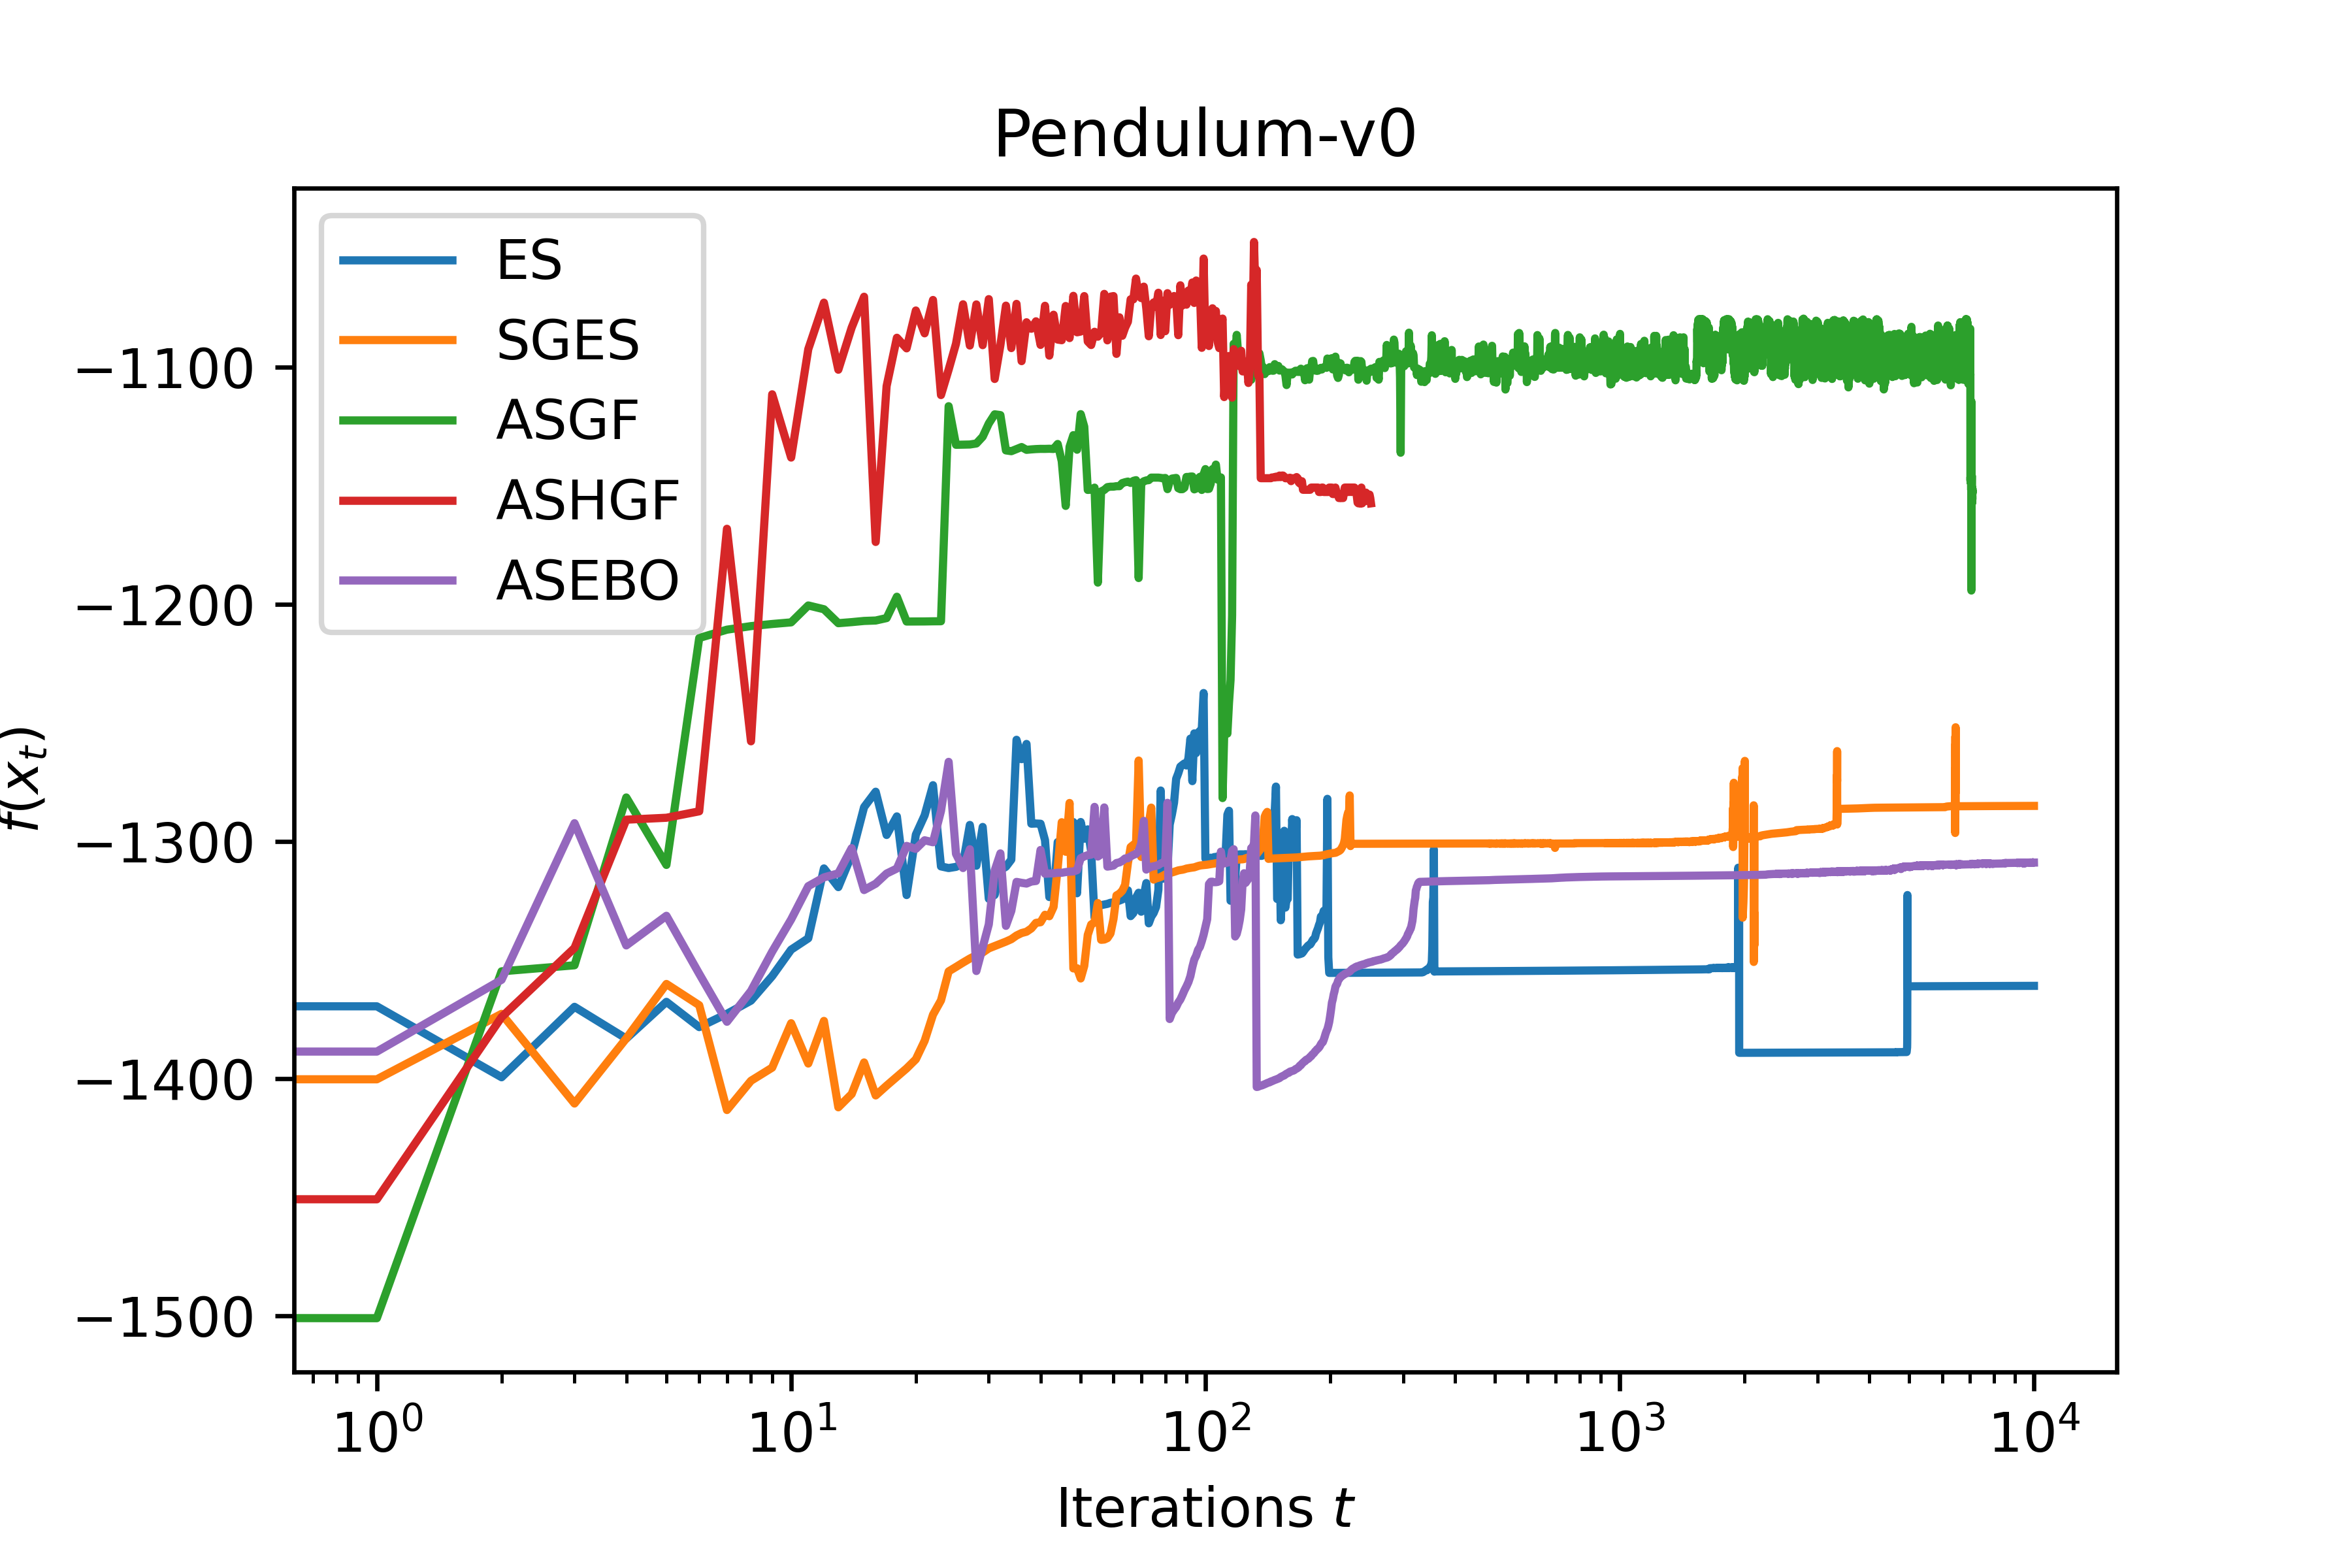
\includegraphics[width=1\textwidth]{figures/RL/RLenvironmentPendulum_convergence_mean.png}
	\end{subfigure}%
	\begin{subfigure}{0.4\textwidth}
		\centering 
		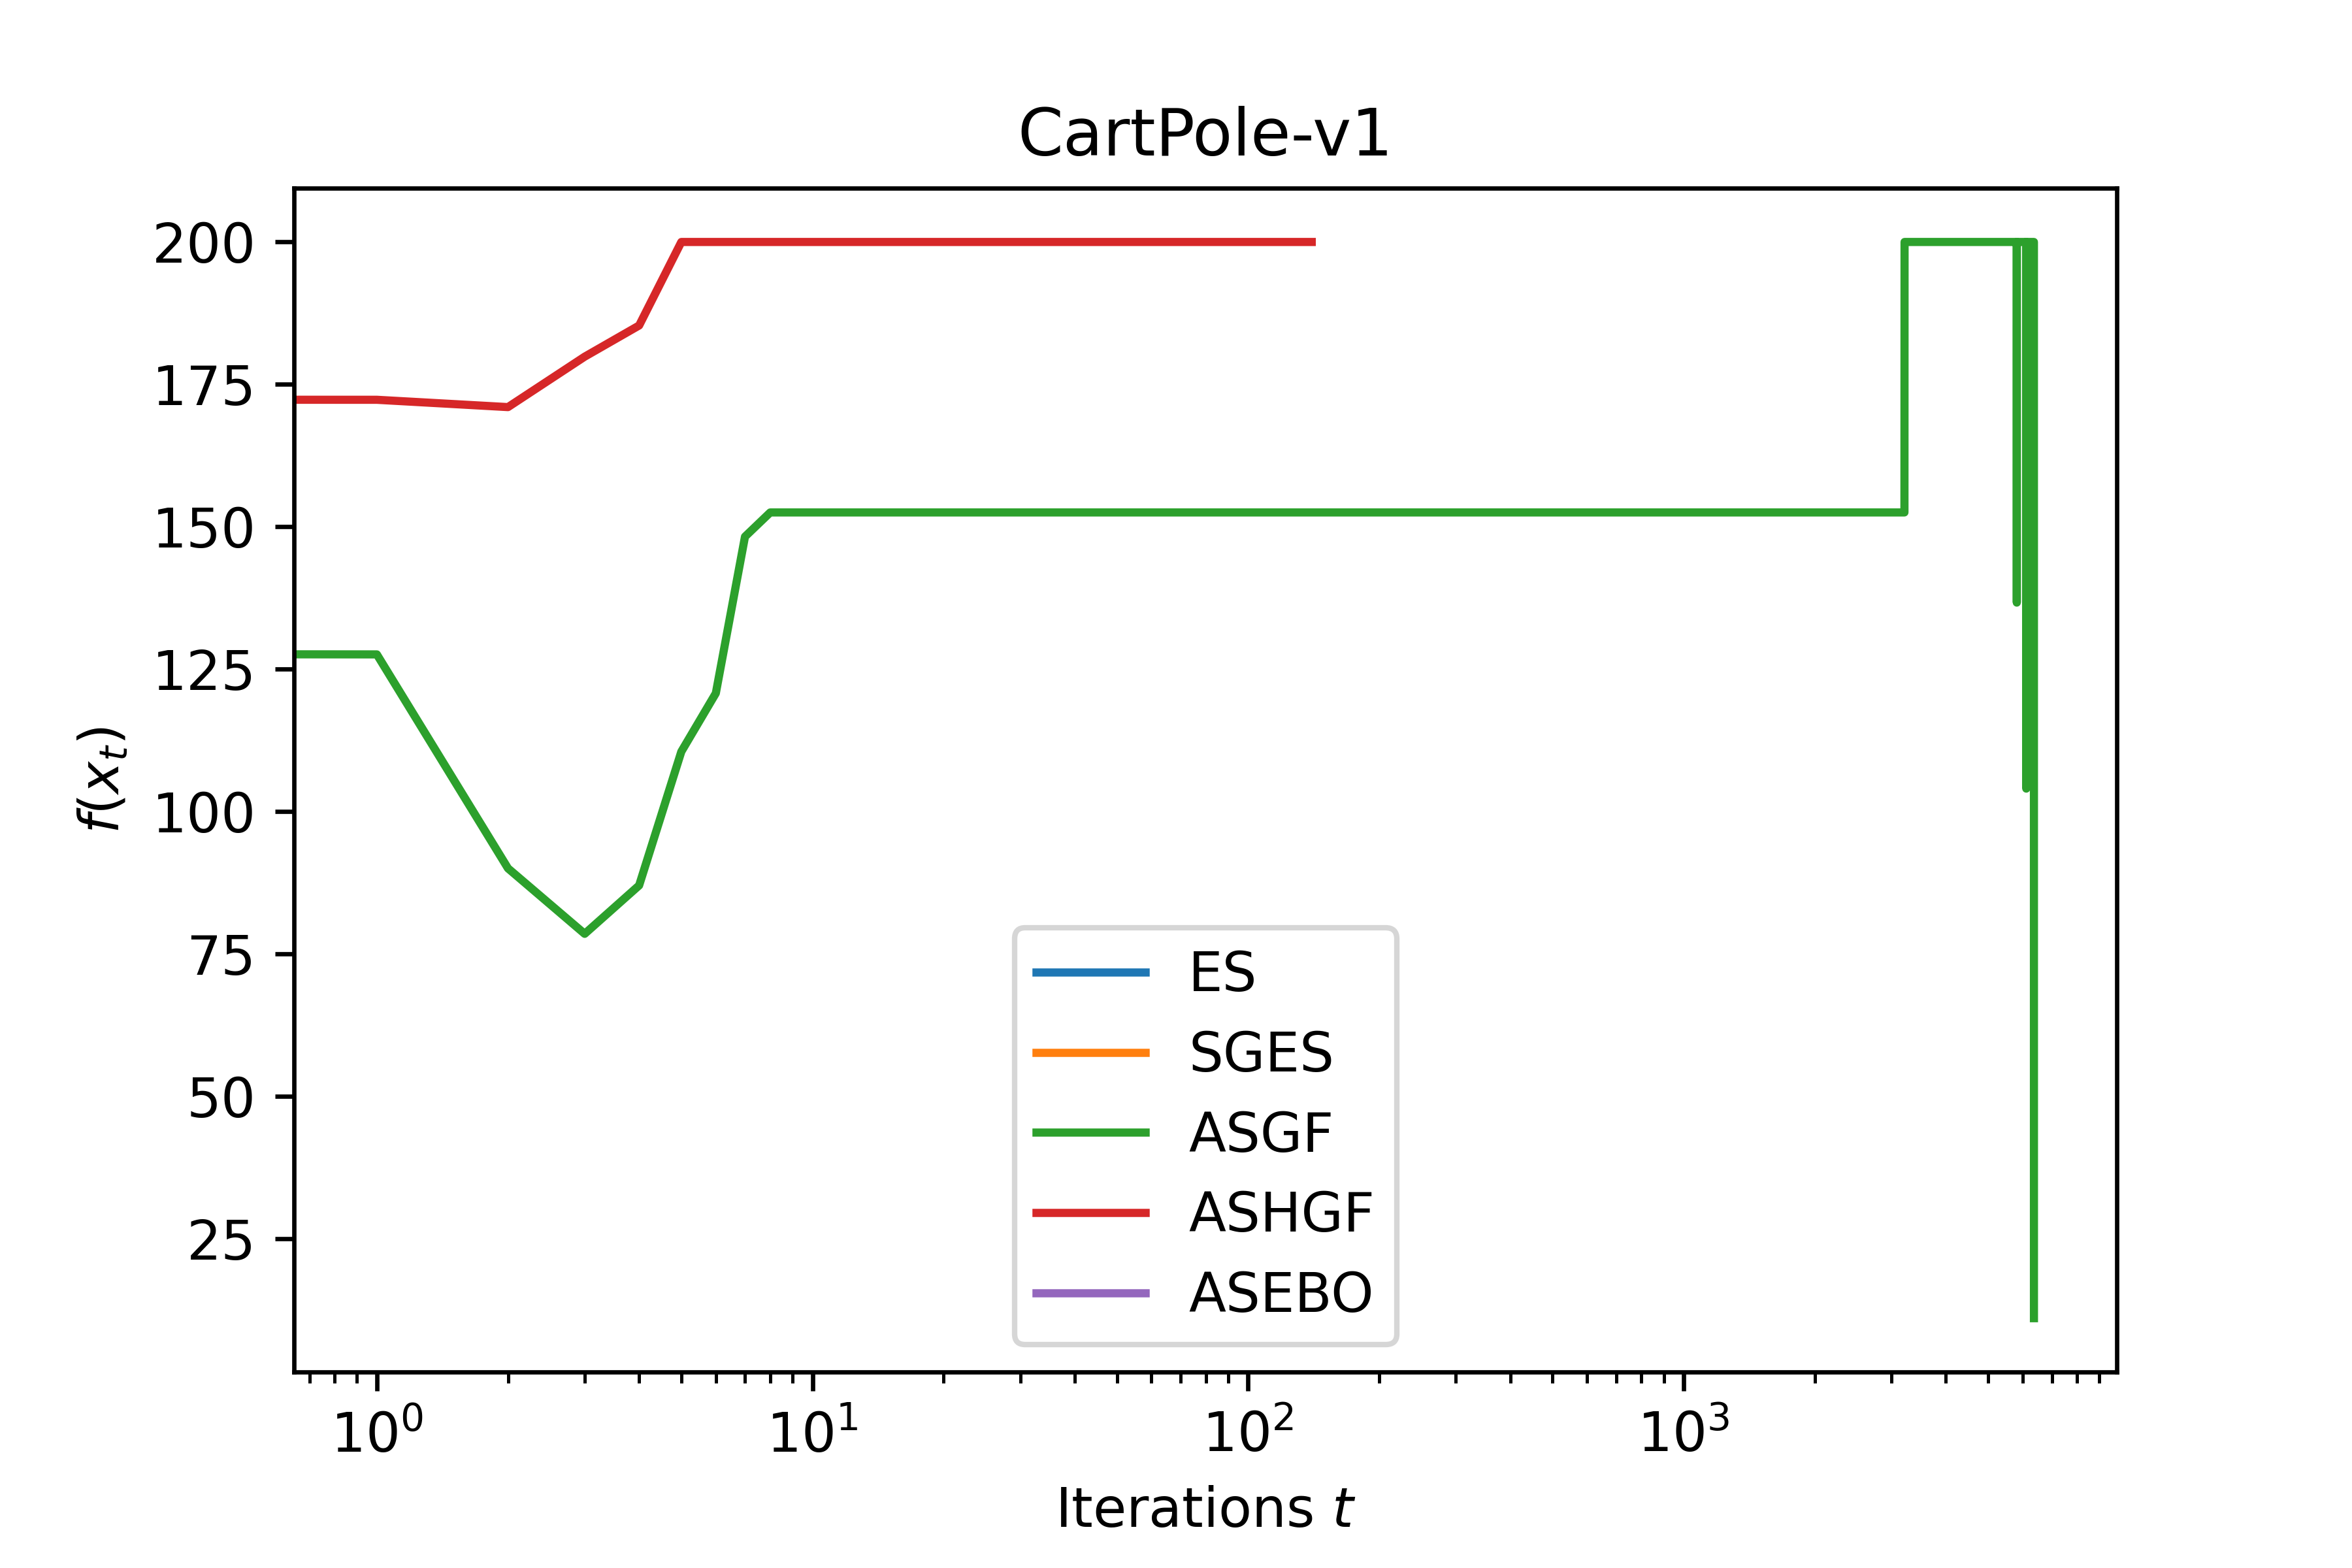
\includegraphics[width=1\textwidth]{figures/RL/RLenvironmentCartPole_convergence_mean.png}
	\end{subfigure}
	\caption[Reinforcement learning results.]{The figures show the average run of the algorithms in two different RL problems with $10$ different random seeds.}
	\label{RLResults}
\end{figure}

As it can be seen, on average the presented algorithm achieves higher rewards and does so faster with respect to the considered state-of-the-art algorithms.